\documentclass[twoside]{book}

% Packages required by doxygen
\usepackage{fixltx2e}
\usepackage{calc}
\usepackage{doxygen}
\usepackage[export]{adjustbox} % also loads graphicx
\usepackage{graphicx}
\usepackage[utf8]{inputenc}
\usepackage{makeidx}
\usepackage{multicol}
\usepackage{multirow}
\PassOptionsToPackage{warn}{textcomp}
\usepackage{textcomp}
\usepackage[nointegrals]{wasysym}
\usepackage[table]{xcolor}

% Font selection
\usepackage[T1]{fontenc}
\usepackage[scaled=.90]{helvet}
\usepackage{courier}
\usepackage{amssymb}
\usepackage{sectsty}
\renewcommand{\familydefault}{\sfdefault}
\allsectionsfont{%
  \fontseries{bc}\selectfont%
  \color{darkgray}%
}
\renewcommand{\DoxyLabelFont}{%
  \fontseries{bc}\selectfont%
  \color{darkgray}%
}
\newcommand{\+}{\discretionary{\mbox{\scriptsize$\hookleftarrow$}}{}{}}

% Page & text layout
\usepackage{geometry}
\geometry{%
  a4paper,%
  top=2.5cm,%
  bottom=2.5cm,%
  left=2.5cm,%
  right=2.5cm%
}
\tolerance=750
\hfuzz=15pt
\hbadness=750
\setlength{\emergencystretch}{15pt}
\setlength{\parindent}{0cm}
\setlength{\parskip}{3ex plus 2ex minus 2ex}
\makeatletter
\renewcommand{\paragraph}{%
  \@startsection{paragraph}{4}{0ex}{-1.0ex}{1.0ex}{%
    \normalfont\normalsize\bfseries\SS@parafont%
  }%
}
\renewcommand{\subparagraph}{%
  \@startsection{subparagraph}{5}{0ex}{-1.0ex}{1.0ex}{%
    \normalfont\normalsize\bfseries\SS@subparafont%
  }%
}
\makeatother

% Headers & footers
\usepackage{fancyhdr}
\pagestyle{fancyplain}
\fancyhead[LE]{\fancyplain{}{\bfseries\thepage}}
\fancyhead[CE]{\fancyplain{}{}}
\fancyhead[RE]{\fancyplain{}{\bfseries\leftmark}}
\fancyhead[LO]{\fancyplain{}{\bfseries\rightmark}}
\fancyhead[CO]{\fancyplain{}{}}
\fancyhead[RO]{\fancyplain{}{\bfseries\thepage}}
\fancyfoot[LE]{\fancyplain{}{}}
\fancyfoot[CE]{\fancyplain{}{}}
\fancyfoot[RE]{\fancyplain{}{\bfseries\scriptsize Generated by Doxygen }}
\fancyfoot[LO]{\fancyplain{}{\bfseries\scriptsize Generated by Doxygen }}
\fancyfoot[CO]{\fancyplain{}{}}
\fancyfoot[RO]{\fancyplain{}{}}
\renewcommand{\footrulewidth}{0.4pt}
\renewcommand{\chaptermark}[1]{%
  \markboth{#1}{}%
}
\renewcommand{\sectionmark}[1]{%
  \markright{\thesection\ #1}%
}

% Indices & bibliography
\usepackage{natbib}
\usepackage[titles]{tocloft}
\setcounter{tocdepth}{3}
\setcounter{secnumdepth}{5}
\makeindex

% Hyperlinks (required, but should be loaded last)
\usepackage{ifpdf}
\ifpdf
  \usepackage[pdftex,pagebackref=true]{hyperref}
\else
  \usepackage[ps2pdf,pagebackref=true]{hyperref}
\fi
\hypersetup{%
  colorlinks=true,%
  linkcolor=blue,%
  citecolor=blue,%
  unicode%
}

% Custom commands
\newcommand{\clearemptydoublepage}{%
  \newpage{\pagestyle{empty}\cleardoublepage}%
}

\usepackage{caption}
\captionsetup{labelsep=space,justification=centering,font={bf},singlelinecheck=off,skip=4pt,position=top}

%===== C O N T E N T S =====

\begin{document}

% Titlepage & ToC
\hypersetup{pageanchor=false,
             bookmarksnumbered=true,
             pdfencoding=unicode
            }
\pagenumbering{roman}
\begin{titlepage}
\vspace*{7cm}
\begin{center}%
{\Large libwebsockets }\\
\vspace*{1cm}
{\large Generated by Doxygen 1.8.11}\\
\end{center}
\end{titlepage}
\clearemptydoublepage
\tableofcontents
\clearemptydoublepage
\pagenumbering{arabic}
\hypersetup{pageanchor=true}

%--- Begin generated contents ---
\chapter{Libwebsockets A\+PI introduction}
\label{index}\hypertarget{index}{}Libwebsockets covers a lot of interesting features for people making embedded servers or clients


\begin{DoxyItemize}
\item http(s) serving and client operation
\item ws(s) serving and client operation
\item http(s) apis for file transfer and upload
\item http P\+O\+ST form handling (including multipart)
\item cookie-\/based sessions
\item account management (including registration, email verification, lost pw etc)
\item strong ssl P\+FS support (A+ on S\+S\+Llabs test)
\end{DoxyItemize}

You can browse by api category \href{modules.html}{\tt here}. 
\chapter{Notes about building lws}
\label{md_README.build}
\hypertarget{md_README.build}{}
\subsection*{Introduction to C\+Make }

C\+Make is a multi-\/platform build tool that can generate build files for many different target platforms. See more info at \href{http://www.cmake.org}{\tt http\+://www.\+cmake.\+org}

C\+Make also allows/recommends you to do \char`\"{}out of source\char`\"{}-\/builds, that is, the build files are separated from your sources, so there is no need to create elaborate clean scripts to get a clean source tree, instead you simply remove your build directory.

Libwebsockets has been tested to build successfully on the following platforms with S\+SL support (both Open\+S\+S\+L/wolf\+S\+SL)\+:


\begin{DoxyItemize}
\item Windows (Visual Studio)
\item Windows (Min\+GW)
\item Linux (x86 and A\+RM)
\item O\+SX
\item Net\+B\+SD
\end{DoxyItemize}

\subsection*{Building the library and test apps }

The project settings used by C\+Make to generate the platform specific build files is called \href{CMakeLists.txt}{\tt C\+Make\+Lists.\+txt}. C\+Make then uses one of its \char`\"{}\+Generators\char`\"{} to output a Visual Studio project or Make file for instance. To see a list of the available generators for your platform, simply run the \char`\"{}cmake\char`\"{} command.

Note that by default Open\+S\+SL will be linked, if you don\textquotesingle{}t want S\+SL support see below on how to toggle compile options.

\subsection*{Building on Unix\+: }


\begin{DoxyEnumerate}
\item Install C\+Make 2.\+8 or greater\+: \href{http://cmake.org/cmake/resources/software.html}{\tt http\+://cmake.\+org/cmake/resources/software.\+html} (Most Unix distributions comes with a packaged version also)
\item Install Open\+S\+SL.
\item Generate the build files (default is Make files)\+: 
\begin{DoxyCode}
1 $ cd /path/to/src
2 $ mkdir build
3 $ cd build
4 $ cmake ..
\end{DoxyCode}

\item Finally you can build using the generated Makefile\+: 
\begin{DoxyCode}
1 $ make && sudo make install
\end{DoxyCode}
 {\bfseries N\+O\+TE}\+: The {\ttfamily build/}{\ttfamily directory can have any name and be located anywhere on your filesystem, and that the argument}..` given to cmake is simply the source directory of {\bfseries libwebsockets} containing the \href{CMakeLists.txt}{\tt C\+Make\+Lists.\+txt} project file. All examples in this file assumes you use \char`\"{}..\char`\"{}
\end{DoxyEnumerate}

{\bfseries N\+O\+T\+E2}\+: A common option you may want to give is to set the install path, same as --prefix= with autotools. It defaults to /usr/local. You can do this by, eg 
\begin{DoxyCode}
1 $ cmake -DCMAKE\_INSTALL\_PREFIX:PATH=/usr .
\end{DoxyCode}


{\bfseries N\+O\+T\+E3}\+: On machines that want libraries in lib64, you can also add the following to the cmake line 
\begin{DoxyCode}
1 -DLIB\_SUFFIX=64
\end{DoxyCode}


{\bfseries N\+O\+T\+E4}\+: If you are building against a non-\/distro Open\+S\+SL (eg, in order to get access to A\+L\+PN support only in newer Open\+S\+SL versions) the nice way to express that in one cmake command is eg, 
\begin{DoxyCode}
1 $ cmake .. -DOPENSSL\_ROOT\_DIR=/usr/local/ssl \(\backslash\)
2          -DCMAKE\_INCLUDE\_DIRECTORIES\_PROJECT\_BEFORE=/usr/local/ssl \(\backslash\)
3          -DLWS\_WITH\_HTTP2=1
\end{DoxyCode}


When you run the test apps using non-\/distro S\+SL, you have to force them to use your libs, not the distro ones 
\begin{DoxyCode}
1 $ LD\_LIBRARY\_PATH=/usr/local/ssl/lib libwebsockets-test-server --ssl
\end{DoxyCode}


To get it to build on latest openssl (2016-\/04-\/10) it needed this approach 
\begin{DoxyCode}
1 cmake .. -DLWS\_WITH\_HTTP2=1 -DLWS\_OPENSSL\_INCLUDE\_DIRS=/usr/local/include/openssl
       -DLWS\_OPENSSL\_LIBRARIES="/usr/local/lib64/libssl.so;/usr/local/lib64/libcrypto.so"
\end{DoxyCode}


{\bfseries N\+O\+T\+E5}\+: To build with debug info and \+\_\+\+D\+E\+B\+UG for lower priority debug messages compiled in, use 
\begin{DoxyCode}
1 $ cmake .. -DCMAKE\_BUILD\_TYPE=DEBUG
\end{DoxyCode}


\subsection*{Quirk of cmake }

When changing cmake options, for some reason the only way to get it to see the changes sometimes is delete the contents of your build directory and do the cmake from scratch.

\subsection*{Building on Windows (Visual Studio) }


\begin{DoxyEnumerate}
\item Install C\+Make 2.\+6 or greater\+: \href{http://cmake.org/cmake/resources/software.html}{\tt http\+://cmake.\+org/cmake/resources/software.\+html}
\item Install Open\+S\+SL binaries. \href{http://www.openssl.org/related/binaries.html}{\tt http\+://www.\+openssl.\+org/related/binaries.\+html}

({\bfseries N\+O\+TE}\+: Preferably in the default location to make it easier for C\+Make to find them)

{\bfseries N\+O\+T\+E2}\+: Be sure that O\+P\+E\+N\+S\+S\+L\+\_\+\+C\+O\+NF environment variable is defined and points at $<$\+Open\+S\+S\+L install=\char`\"{}\char`\"{} location$>$=\char`\"{}\char`\"{}$>$.cfg
\item Generate the Visual studio project by opening the Visual Studio cmd prompt\+:
\end{DoxyEnumerate}


\begin{DoxyCode}
1 cd <path to src>
2 md build
3 cd build
4 cmake -G "Visual Studio 10" ..
\end{DoxyCode}


({\bfseries N\+O\+TE}\+: There is also a cmake-\/gui available on Windows if you prefer that)

{\bfseries N\+O\+T\+E2}\+: See this link to find out the version number corresponding to your Visual Studio edition\+: \href{http://superuser.com/a/194065}{\tt http\+://superuser.\+com/a/194065}


\begin{DoxyEnumerate}
\item Now you should have a generated Visual Studio Solution in your {\ttfamily $<$path to src$>$/build} directory, which can be used to build.
\item Some additional deps may be needed
\begin{DoxyItemize}
\item iphlpapi.\+lib
\item psapi.\+lib
\item userenv.\+lib
\end{DoxyItemize}
\item If you\textquotesingle{}re using libuv, you must make sure to compile libuv with the same multithread-\/dll / Mtd attributes as libwebsockets itself
\end{DoxyEnumerate}

\subsection*{Building on Windows (Min\+GW) }


\begin{DoxyEnumerate}
\item Install Min\+GW\+: \href{http://sourceforge.net/projects/mingw/files}{\tt http\+://sourceforge.\+net/projects/mingw/files}

({\bfseries N\+O\+TE}\+: Preferably in the default location C\+:)
\item Fix up Min\+GW headers

a) Add the following lines to C\+:.h\+: 
\begin{DoxyCode}
1 #if(\_WIN32\_WINNT >= 0x0600)
2 
3 typedef struct pollfd \{
4 
5         SOCKET  fd;
6         SHORT   events;
7         SHORT   revents;
8 
9 \} WSAPOLLFD, *PWSAPOLLFD, FAR *LPWSAPOLLFD;
10 
11 WINSOCK\_API\_LINKAGE int WSAAPI WSAPoll(LPWSAPOLLFD fdArray, ULONG fds, INT timeout);
12 
13 #endif // (\_WIN32\_WINNT >= 0x0600)
\end{DoxyCode}
 b) Create C\+:.h and copy and paste the content from following link into it\+:

\href{http://wine-unstable.sourcearchive.com/documentation/1.1.32/mstcpip_8h-source.html}{\tt http\+://wine-\/unstable.\+sourcearchive.\+com/documentation/1.\+1.\+32/mstcpip\+\_\+8h-\/source.\+html}
\item Install C\+Make 2.\+6 or greater\+: \href{http://cmake.org/cmake/resources/software.html}{\tt http\+://cmake.\+org/cmake/resources/software.\+html}
\item Install Open\+S\+SL binaries. \href{http://www.openssl.org/related/binaries.html}{\tt http\+://www.\+openssl.\+org/related/binaries.\+html}

({\bfseries N\+O\+TE}\+: Preferably in the default location to make it easier for C\+Make to find them)

{\bfseries N\+O\+T\+E2}\+: Be sure that O\+P\+E\+N\+S\+S\+L\+\_\+\+C\+O\+NF environment variable is defined and points at $<$\+Open\+S\+S\+L install=\char`\"{}\char`\"{} location$>$=\char`\"{}\char`\"{}$>$.cfg
\item Generate the build files (default is Make files) using M\+S\+YS shell\+: 
\begin{DoxyCode}
1 $ cd /drive/path/to/src
2 $ mkdir build
3 $ cd build
4 $ cmake -G "MSYS Makefiles" -DCMAKE\_INSTALL\_PREFIX=C:/MinGW ..
\end{DoxyCode}
 ({\bfseries N\+O\+TE}\+: The {\ttfamily build/}{\ttfamily directory can have any name and be located anywhere on your filesystem, and that the argument}..` given to cmake is simply the source directory of {\bfseries libwebsockets} containing the \href{CMakeLists.txt}{\tt C\+Make\+Lists.\+txt} project file. All examples in this file assumes you use \char`\"{}..\char`\"{})

{\bfseries N\+O\+T\+E2}\+: To generate build files allowing to create libwebsockets binaries with debug information set the C\+M\+A\+K\+E\+\_\+\+B\+U\+I\+L\+D\+\_\+\+T\+Y\+PE flag to D\+E\+B\+UG\+: 
\begin{DoxyCode}
1 $ cmake -G "MSYS Makefiles" -DCMAKE\_INSTALL\_PREFIX=C:/MinGW -DCMAKE\_BUILD\_TYPE=DEBUG ..
\end{DoxyCode}

\item Finally you can build using the generated Makefile and get the results deployed into your Min\+GW installation\+:
\end{DoxyEnumerate}


\begin{DoxyCode}
1 $ make
2 $ make install
\end{DoxyCode}


\subsection*{Setting compile options }

To set compile time flags you can either use one of the C\+Make gui applications or do it via command line.

\subsection*{Command line }

To list avaialable options (ommit the H if you don\textquotesingle{}t want the help text)\+: \begin{DoxyVerb}    cmake -LH ..
\end{DoxyVerb}


Then to set an option and build (for example turn off S\+SL support)\+: \begin{DoxyVerb}    cmake -DLWS_WITH_SSL=0 ..
\end{DoxyVerb}
 or cmake -\/\+D\+L\+W\+S\+\_\+\+W\+I\+T\+H\+\_\+\+S\+SL\+:B\+O\+OL=O\+FF ..

\subsection*{Building on mbed3 }

M\+B\+E\+D3 is a non-\/posix embedded OS targeted on Cortex M class chips.

\href{https://www.mbed.com/}{\tt https\+://www.\+mbed.\+com/}

It\textquotesingle{}s quite unlike any other Posixy platform since the OS is linked statically in with lws to form one binary.

At the minute server-\/only is supported and due to bugs in mbed3 network support, the port is of alpha quality. However it can serve the test html, favicon.\+ico and logo png and may be able to make ws connections. The binary for that including the OS, test app, lws and all the assets is only 117\+KB.

0) Today mbed3 only properly works on F\+R\+DM K64F \$35 Freescale Dev Board with 1\+MB Flash, 256\+KB S\+R\+AM and Ethernet.

\href{http://www.freescale.com/products/arm-processors/kinetis-cortex-m/k-series/k6x-ethernet-mcus/freescale-freedom-development-platform-for-kinetis-k64-k63-and-k24-mcus:FRDM-K64F}{\tt http\+://www.\+freescale.\+com/products/arm-\/processors/kinetis-\/cortex-\/m/k-\/series/k6x-\/ethernet-\/mcus/freescale-\/freedom-\/development-\/platform-\/for-\/kinetis-\/k64-\/k63-\/and-\/k24-\/mcus\+:\+F\+R\+D\+M-\/\+K64F}

1) Get a working mbed3 environment with arm-\/none-\/eabi-\/cs toolchain (available in Fedora, Ubuntu and other distros)

2) Confirm you can build things using yotta by following the getting started guide here

\href{https://docs.mbed.com/docs/getting-started-mbed-os/en/latest/}{\tt https\+://docs.\+mbed.\+com/docs/getting-\/started-\/mbed-\/os/en/latest/}

3)

git clone \href{https://github.com/warmcat/lws-test-server}{\tt https\+://github.\+com/warmcat/lws-\/test-\/server}

and cd into it

4) mkdir -\/p yotta\+\_\+modules ; cd yotta\+\_\+modules

5) git clone \href{https://github.com/warmcat/libwebsockets}{\tt https\+://github.\+com/warmcat/libwebsockets} ; mv libwebsockets websockets ; cd ..

6) yotta target frdm-\/k64f-\/gcc

7) yotta install

8) yotta build

\subsection*{Unix G\+UI }

If you have a curses-\/enabled build you simply type\+: (not all packages include this, my debian install does not for example). \begin{DoxyVerb}    ccmake
\end{DoxyVerb}


\subsection*{Windows G\+UI }

On windows C\+Make comes with a gui application\+: Start -\/$>$ Programs -\/$>$ C\+Make -\/$>$ C\+Make (cmake-\/gui)

\subsection*{wolf\+S\+S\+L/\+Cya\+S\+SL replacement for Open\+S\+SL }

wolf\+S\+S\+L/\+Cya\+S\+SL is a lightweight S\+SL library targeted at embedded systems\+: \href{https://www.wolfssl.com/wolfSSL/Products-wolfssl.html}{\tt https\+://www.\+wolfssl.\+com/wolf\+S\+S\+L/\+Products-\/wolfssl.\+html}

It contains a Open\+S\+SL compatibility layer which makes it possible to pretty much link to it instead of Open\+S\+SL, giving a much smaller footprint.

{\bfseries N\+O\+TE}\+: wolfssl needs to be compiled using the {\ttfamily -\/-\/enable-\/opensslextra} flag for this to work.

\subsection*{Compiling libwebsockets with wolf\+S\+SL }


\begin{DoxyCode}
1 cmake .. -DLWS\_USE\_WOLFSSL=1 \(\backslash\)
2          -DLWS\_WOLFSSL\_INCLUDE\_DIRS=/path/to/wolfssl \(\backslash\)
3          -DLWS\_WOLFSSL\_LIBRARIES=/path/to/wolfssl/wolfssl.a ..
\end{DoxyCode}


{\bfseries N\+O\+TE}\+: On windows use the .lib file extension for {\ttfamily L\+W\+S\+\_\+\+W\+O\+L\+F\+S\+S\+L\+\_\+\+L\+I\+B\+R\+A\+R\+I\+ES} instead.

\subsection*{Compiling libwebsockets with Cya\+S\+SL }


\begin{DoxyCode}
1 cmake .. -DLWS\_USE\_CYASSL=1 \(\backslash\)
2          -DLWS\_CYASSL\_INCLUDE\_DIRS=/path/to/cyassl \(\backslash\)
3          -DLWS\_CYASSL\_LIBRARIES=/path/to/wolfssl/cyassl.a ..
\end{DoxyCode}


{\bfseries N\+O\+TE}\+: On windows use the .lib file extension for {\ttfamily L\+W\+S\+\_\+\+C\+Y\+A\+S\+S\+L\+\_\+\+L\+I\+B\+R\+A\+R\+I\+ES} instead.

\subsection*{Compiling libwebsockets with Polar\+S\+SL }

Caution... at some point Polar\+S\+SL became Mbed\+T\+LS. But it did not happen all at once. The name changed first then at mbed\+T\+LS 2.\+0 the apis changed. So eg in Fedora 22, there is an \char`\"{}mbedtls\char`\"{} package which is actually using polarssl for the include dir and polarssl apis... this should be treated as polarssl then.

Example config for this case is 
\begin{DoxyCode}
1 cmake .. -DLWS\_USE\_POLARSSL=1 -DLWS\_POLARSSL\_LIBRARIES=/usr/lib64/libmbedtls.so \(\backslash\)
2          -DLWS\_POLARSSL\_INCLUDE\_DIRS=/usr/include/polarssl/
\end{DoxyCode}


\subsection*{Building plugins outside of lws itself }

The directory ./plugin-\/standalone/ shows how easy it is to create plugins outside of lws itself. First build lws itself with -\/\+D\+L\+W\+S\+\_\+\+W\+I\+T\+H\+\_\+\+P\+L\+U\+G\+I\+NS, then use the same flow to build the standalone plugin 
\begin{DoxyCode}
1 cd ./plugin-standalone
2 mkdir build
3 cd build
4 cmake ..
5 make && sudo make install
\end{DoxyCode}


if you changed the default plugin directory when you built lws, you must also give the same arguments to cmake here (eg, {\ttfamily -\/\+D\+C\+M\+A\+K\+E\+\_\+\+I\+N\+S\+T\+A\+L\+L\+\_\+\+P\+R\+E\+F\+IX\+:P\+A\+TH=/usr/something/else...} )

Otherwise if you run lwsws or libwebsockets-\/test-\/server-\/v2.\+0, it will now find the additional plugin \char`\"{}libprotocol\+\_\+example\+\_\+standalone.\+so\char`\"{} 
\begin{DoxyCode}
1 lwsts[21257]:   Plugins:
2 lwsts[21257]:    libprotocol\_dumb\_increment.so
3 lwsts[21257]:    libprotocol\_example\_standalone.so
4 lwsts[21257]:    libprotocol\_lws\_mirror.so
5 lwsts[21257]:    libprotocol\_lws\_server\_status.so
6 lwsts[21257]:    libprotocol\_lws\_status.so
\end{DoxyCode}
 If you have multiple vhosts, you must enable plugins at the vhost additionally, discovered plugins are not enabled automatically for security reasons. You do this using info-\/$>$pvo or for lwsws, in the J\+S\+ON config.

\subsection*{Reproducing H\+T\+T\+P2.\+0 tests }

You must have built and be running lws against a version of openssl that has A\+L\+PN / N\+PN. Most distros still have older versions. You\textquotesingle{}ll know it\textquotesingle{}s right by seeing 
\begin{DoxyCode}
1 lwsts[4752]:  Compiled with OpenSSL support
2 lwsts[4752]:  Using SSL mode
3 lwsts[4752]:  HTTP2 / ALPN enabled
\end{DoxyCode}
 at lws startup.

For non-\/\+S\+SL H\+T\+T\+P2.\+0 upgrade 
\begin{DoxyCode}
1 $ nghttp -nvasu http://localhost:7681/test.htm
\end{DoxyCode}
 For S\+SL / A\+L\+PN H\+T\+T\+P2.\+0 upgrade 
\begin{DoxyCode}
1 $ nghttp -nvas https://localhost:7681/test.html
\end{DoxyCode}


\subsection*{Cross compiling }

To enable cross-\/compiling {\bfseries libwebsockets} using C\+Make you need to create a \char`\"{}\+Toolchain file\char`\"{} that you supply to C\+Make when generating your build files. C\+Make will then use the cross compilers and build paths specified in this file to look for dependencies and such.

{\bfseries Libwebsockets} includes an example toolchain file \href{cross-arm-linux-gnueabihf.cmake}{\tt cross-\/arm-\/linux-\/gnueabihf.\+cmake} you can use as a starting point.

The commandline to configure for cross with this would look like 
\begin{DoxyCode}
1 $ cmake .. -DCMAKE\_INSTALL\_PREFIX:PATH=/usr \(\backslash\)
2          -DCMAKE\_TOOLCHAIN\_FILE=../cross-arm-linux-gnueabihf.cmake \(\backslash\)
3          -DWITHOUT\_EXTENSIONS=1 -DWITH\_SSL=0
\end{DoxyCode}
 The example shows how to build with no external cross lib dependencies, you need to provide the cross libraries otherwise.

{\bfseries N\+O\+TE}\+: start from an E\+M\+P\+TY build directory if you had a non-\/cross build in there before the settings will be cached and your changes ignored.

Additional information on cross compilation with C\+Make\+: \href{http://www.vtk.org/Wiki/CMake_Cross_Compiling}{\tt http\+://www.\+vtk.\+org/\+Wiki/\+C\+Make\+\_\+\+Cross\+\_\+\+Compiling}

\subsection*{Memory efficiency }

Embedded server-\/only configuration without extensions (ie, no compression on websocket connections), but with full v13 websocket features and http server, built on A\+RM Cortex-\/\+A9\+:

Update at 8dac94d (2013-\/02-\/18) 
\begin{DoxyCode}
1 $ ./configure --without-client --without-extensions --disable-debug --without-daemonize
2 
3 Context Creation, 1024 fd limit[2]:   16720 (includes 12 bytes per fd)
4 Per-connection [3]:                      72 bytes, +1328 during headers
5 
6 .text   .rodata .data   .bss
7 11512   2784    288     4
\end{DoxyCode}
 This shows the impact of the major configuration with/without options at 13ba5bbc633ea962d46d using Ubuntu A\+RM on a Panda\+Board ES.

These are accounting for static allocations from the library elf, there are additional dynamic allocations via malloc. These are a bit old now but give the right idea for relative \char`\"{}expense\char`\"{} of features.

Static allocations, A\+R\+M9

\tabulinesep=1mm
\begin{longtabu} spread 0pt [c]{*5{|X[-1]}|}
\hline
\rowcolor{\tableheadbgcolor}{\bf }&{\bf .text }&{\bf .rodata }&{\bf .data }&{\bf .bss  }\\\cline{1-5}
\endfirsthead
\hline
\endfoot
\hline
\rowcolor{\tableheadbgcolor}{\bf }&{\bf .text }&{\bf .rodata }&{\bf .data }&{\bf .bss  }\\\cline{1-5}
\endhead
All (no without) &35024 &9940 &336 &4104 \\\cline{1-5}
without client &25684 &7144 &336 &4104 \\\cline{1-5}
without client, exts &21652 &6288 &288 &4104 \\\cline{1-5}
without client, exts, debug\mbox{[}1\mbox{]} &19756 &3768 &288 &4104 \\\cline{1-5}
without server &30304 &8160 &336 &4104 \\\cline{1-5}
without server, exts &25382 &7204 &288 &4104 \\\cline{1-5}
without server, exts, debug\mbox{[}1\mbox{]} &23712 &4256 &288 &4104 \\\cline{1-5}
\end{longtabu}
\mbox{[}1\mbox{]} {\ttfamily -\/-\/disable-\/debug} only removes messages below {\ttfamily lwsl\+\_\+notice}. Since that is the default logging level the impact is not noticeable, error, warn and notice logs are all still there.

\mbox{[}2\mbox{]} {\ttfamily 1024} fd per process is the default limit (set by ulimit) in at least Fedora and Ubuntu. You can make significant savings tailoring this to actual expected peak fds, ie, at a limit of {\ttfamily 20}, context creation allocation reduces to {\ttfamily 4432 + 240 = 4672})

\mbox{[}3\mbox{]} known header content is freed after connection establishment 
\chapter{Debugging problems}
\label{md_README.problems}
\hypertarget{md_README.problems}{}
\subsection*{Library is a component }

As a library, lws is just a component in a bigger application.

Many users are able to share their sources, but others decide not to, for \char`\"{}commerical advantage\char`\"{} or whatever.

This makes answering questions like \char`\"{}what is wrong with my code I am not
going to show you?\char`\"{} very difficult.

Even if it\textquotesingle{}s clear there is a problem somewhere, it cannot be understood or reproduced by anyone else if it needs user code that isn\textquotesingle{}t provided.

The biggest question is, \char`\"{}is this an lws problem actually\char`\"{}?

\subsection*{Use the test apps as sanity checks }

The test server and client are extremely useful for sanity checks and debugging guidance.


\begin{DoxyItemize}
\item test apps work on your platform, then either
\begin{DoxyItemize}
\item your user code is broken, align it to how the test apps work, or,
\item something from your code is required to show an lws problem, provide a minimal patch on a test app so it can be reproduced
\end{DoxyItemize}
\item test apps break on your platform, but work on, eg, x86\+\_\+64, either
\begin{DoxyItemize}
\item toolchain or platform-\/specific (eg, OS) issue, or
\item lws platform support issue
\end{DoxyItemize}
\item test apps break everywhere
\begin{DoxyItemize}
\item sounds like lws problem, info to reproduce and / or a patch is appreciated 
\end{DoxyItemize}
\end{DoxyItemize}
\chapter{Notes about lwsws}
\label{md_README.lwsws}
\hypertarget{md_README.lwsws}{}
\subsection*{Libwebsockets Web Server }

lwsws is an implementation of a very lightweight, ws-\/capable generic web server, which uses libwebsockets to implement everything underneath.

\subsection*{Build }

Just enable -\/\+D\+L\+W\+S\+\_\+\+W\+I\+T\+H\+\_\+\+L\+W\+S\+WS=1 at cmake-\/time.

It enables libuv and plugin support automatically.

\subsection*{Configuration }

lwsws uses J\+S\+ON config files, they\textquotesingle{}re pure J\+S\+ON but \# may be used to turn the rest of the line into a comment.

There\textquotesingle{}s also a single substitution, if a string contains \char`\"{}\+\_\+lws\+\_\+ddir\+\_\+\char`\"{}, then that is replaced with the L\+WS install data directory path, eg, \char`\"{}/usr/share\char`\"{} or whatever was set when L\+WS was built + installed. That lets you refer to installed paths without having to change the config if your install path was different.

There is a single file intended for global settings

/etc/lwsws/conf 
\begin{DoxyCode}
1 # these are the server global settings
2 # stuff related to vhosts should go in one
3 # file per vhost in ../conf.d/
4 
5 \{
6   "global": \{
7    "uid": "48",  # apache user
8    "gid": "48",  # apache user
9    "count-threads": "1",
10    "server-string": "myserver v1", # returned in http headers
11    "init-ssl": "yes"
12  \}
13 \}
\end{DoxyCode}
 and a config directory intended to take one file per vhost

/etc/lwsws/conf.d/warmcat.\+com 
\begin{DoxyCode}
1 \{
2         "vhosts": [\{
3                 "name": "warmcat.com",
4                 "port": "443",
5                 "interface": "eth0",  # optional
6                 "host-ssl-key": "/etc/pki/tls/private/warmcat.com.key",  # if given enable ssl
7                 "host-ssl-cert": "/etc/pki/tls/certs/warmcat.com.crt",
8                 "host-ssl-ca": "/etc/pki/tls/certs/warmcat.com.cer",
9                 "mounts": [\{  # autoserve
10                         "mountpoint": "/",
11                         "origin": "file:///var/www/warmcat.com",
12                         "default": "index.html"
13                 \}]
14         \}]
15 \}
\end{DoxyCode}
 To get started quickly, an example config reproducing the old test server on port 7681, non-\/\+S\+SL is provided. To set it up 
\begin{DoxyCode}
1 # mkdir -p /etc/lwsws/conf.d /var/log/lwsws
2 # cp ./lwsws/etc-lwsws-conf-EXAMPLE /etc/lwsws/conf
3 # cp ./lwsws/etc-lwsws-conf.d-localhost-EXAMPLE /etc/lwsws/conf.d/test-server
4 # sudo lwsws
\end{DoxyCode}
 \subsection*{Vhosts }

One server can run many vhosts, where S\+SL is in use S\+NI is used to match the connection to a vhost and its vhost-\/specific S\+SL keys during S\+SL negotiation.

Listing multiple vhosts looks something like this 
\begin{DoxyCode}
1 \{
2  "vhosts": [ \{
3      "name": "localhost",
4      "port": "443",
5      "host-ssl-key":  "/etc/pki/tls/private/libwebsockets.org.key",
6      "host-ssl-cert": "/etc/pki/tls/certs/libwebsockets.org.crt",
7      "host-ssl-ca":   "/etc/pki/tls/certs/libwebsockets.org.cer",
8      "mounts": [\{
9        "mountpoint": "/",
10        "origin": "file:///var/www/libwebsockets.org",
11        "default": "index.html"
12        \}, \{
13         "mountpoint": "/testserver",
14         "origin": "file:///usr/local/share/libwebsockets-test-server",
15         "default": "test.html"
16        \}],
17      # which protocols are enabled for this vhost, and optional
18      # vhost-specific config options for the protocol
19      #
20      "ws-protocols": [\{
21        "warmcat,timezoom": \{
22          "status": "ok"
23        \}
24      \}]
25     \},
26     \{
27     "name": "localhost",
28     "port": "7681",
29      "host-ssl-key":  "/etc/pki/tls/private/libwebsockets.org.key",
30      "host-ssl-cert": "/etc/pki/tls/certs/libwebsockets.org.crt",
31      "host-ssl-ca":   "/etc/pki/tls/certs/libwebsockets.org.cer",
32      "mounts": [\{
33        "mountpoint": "/",
34        "origin": ">https://localhost"
35      \}]
36    \},
37     \{
38     "name": "localhost",
39     "port": "80",
40      "mounts": [\{
41        "mountpoint": "/",
42        "origin": ">https://localhost"
43      \}]
44    \}
45 
46   ]
47 \}
\end{DoxyCode}


That sets up three vhosts all called \char`\"{}localhost\char`\"{} on ports 443 and 7681 with S\+SL, and port 80 without S\+SL but with a forced redirect to \href{https://localhost}{\tt https\+://localhost}

\subsection*{Vhost name and port }

The vhost name field is used to match on incoming S\+NI or Host\+: header, so it must always be the host name used to reach the vhost externally.


\begin{DoxyItemize}
\item Vhosts may have the same name and different ports, these will each create a listening socket on the appropriate port.
\item Vhosts may also have the same port and different name\+: these will be treated as true vhosts on one listening socket and the active vhost decided at S\+SL negotiation time (via S\+NI) or if no S\+SL, then after the Host\+: header from the client has been parsed.
\end{DoxyItemize}

\subsection*{Protocols }

Vhosts by default have available the union of any initial protocols from context creation time, and any protocols exposed by plugins.

Vhosts can select which plugins they want to offer and give them per-\/vhost settings using this syntax 
\begin{DoxyCode}
1 "ws-protocols": [\{
2   "warmcat-timezoom": \{
3     "status": "ok"
4   \}
5 \}]
\end{DoxyCode}


The \char`\"{}x\char`\"{}\+:\char`\"{}y\char`\"{} parameters like \char`\"{}status\char`\"{}\+:\char`\"{}ok\char`\"{} are made available to the protocol during its per-\/vhost L\+W\+S\+\_\+\+C\+A\+L\+L\+B\+A\+C\+K\+\_\+\+P\+R\+O\+T\+O\+C\+O\+L\+\_\+\+I\+N\+IT ( is a pointer to a linked list of struct \hyperlink{structlws__protocol__vhost__options}{lws\+\_\+protocol\+\_\+vhost\+\_\+options} containing the name and value pointers).

To indicate that a protocol should be used when no Protocol\+: header is sent by the client, you can use \char`\"{}default\char`\"{}\+: \char`\"{}1\char`\"{} 
\begin{DoxyCode}
1 "ws-protocols": [\{
2   "warmcat-timezoom": \{
3     "status": "ok",
4     "default": "1"
5   \}
6 \}]
\end{DoxyCode}


\subsection*{Other vhost options }


\begin{DoxyItemize}
\item If the three options {\ttfamily host-\/ssl-\/cert}, {\ttfamily host-\/ssl-\/ca} and {\ttfamily host-\/ssl-\/key} are given, then the vhost supports S\+SL.
\end{DoxyItemize}

Each vhost may have its own certs, S\+NI is used during the initial connection negotiation to figure out which certs to use by the server name it\textquotesingle{}s asking for from the request D\+NS name.


\begin{DoxyItemize}
\item {\ttfamily keeplive-\/timeout} (in secs) defaults to 60 for lwsws, it may be set as a vhost option
\item {\ttfamily interface} lets you specify which network interface to listen on, if not given listens on all
\item \char`\"{}`unix-\/socket`\char`\"{}\+: \char`\"{}1\char`\"{} causes the unix socket specified in the interface option to be used instead of an I\+N\+ET socket
\item \char`\"{}`sts`\char`\"{}\+: \char`\"{}1\char`\"{} causes lwsws to send a Strict Transport Security header with responses that informs the client he should never accept to connect to this address using http. This is needed to get the A+ security rating from S\+SL Labs for your server.
\item \char`\"{}`access-\/log`\char`\"{}\+: \char`\"{}filepath\char`\"{} sets where apache-\/compatible access logs will be written
\item {\ttfamily \char`\"{}enable-\/client-\/ssl\char`\"{}}\+: {\ttfamily \char`\"{}1\char`\"{}} enables the vhost\textquotesingle{}s client S\+SL context, you will need this if you plan to create client conections on the vhost that will use S\+SL. You don\textquotesingle{}t need it if you only want http / ws client connections.
\item \char`\"{}`ciphers`\char`\"{}\+: \char`\"{}$<$cipher list$>$\char`\"{} sets the allowed list of ciphers and key exchange protocols for the vhost. The default list is restricted to only those providing P\+FS (Perfect Forward Secrecy) on the author\textquotesingle{}s Fedora system.
\end{DoxyItemize}

If you need to allow weaker ciphers,you can provide an alternative list here per-\/vhost.


\begin{DoxyItemize}
\item \char`\"{}`ecdh-\/curve`\char`\"{}\+: \char`\"{}$<$curve name$>$\char`\"{} The default ecdh curve is \char`\"{}prime256v1\char`\"{}, but you can override it here, per-\/vhost
\item \char`\"{}`noipv6`\char`\"{}\+: \char`\"{}on\char`\"{} Disable ipv6 completely for this vhost
\item \char`\"{}`ipv6only`\char`\"{}\+: \char`\"{}on\char`\"{} Only allow ipv6 on this vhost / \char`\"{}off\char`\"{} only allow ipv4 on this vhost
\item \char`\"{}`ssl-\/option-\/set`\char`\"{}\+: \char`\"{}$<$decimal$>$\char`\"{} Sets the S\+SL option flag value for the vhost. It may be used multiple times and OR\textquotesingle{}s the flags together.
\end{DoxyItemize}

The values are derived from /usr/include/openssl/ssl.h 
\begin{DoxyCode}
1 # define SSL\_OP\_NO\_TLSv1\_1                               0x10000000L
\end{DoxyCode}


would equate to


\begin{DoxyCode}
1 "`ssl-option-set`": "268435456"
\end{DoxyCode}

\begin{DoxyItemize}
\item \char`\"{}`ssl-\/option-\/clear\textquotesingle{}\char`\"{}\+: \char`\"{}$<$decimal$>$\char`\"{} Clears the S\+SL option flag value for the vhost. It may be used multiple times and OR\textquotesingle{}s the flags together.
\end{DoxyItemize}

\subsection*{Mounts }

Where mounts are given in the vhost definition, then directory contents may be auto-\/served if it matches the mountpoint.

Mount protocols are used to control what kind of translation happens


\begin{DoxyItemize}
\item \href{file://}{\tt file\+://} serve the uri using the remainder of the url past the mountpoint based on the origin directory.
\end{DoxyItemize}

Eg, with this mountpoint 
\begin{DoxyCode}
1 \{
2  "mountpoint": "/",
3  "origin": "file:///var/www/mysite.com",
4  "default": "/"
5 \}
\end{DoxyCode}
 The uri /file.jpg would serve /var/www/mysite.com/file.\+jpg, since / matched.


\begin{DoxyItemize}
\item $^\wedge$http\+:// or $^\wedge$https\+:// these cause any url matching the mountpoint to issue a redirect to the origin url
\item cgi\+:// this causes any matching url to be given to the named cgi, eg 
\begin{DoxyCode}
1 \{
2  "mountpoint": "/git",
3  "origin": "cgi:///var/www/cgi-bin/cgit",
4  "default": "/"
5 \}, \{
6  "mountpoint": "/cgit-data",
7  "origin": "file:///usr/share/cgit",
8  "default": "/"
9 \},
\end{DoxyCode}
 would cause the url /git/myrepo to pass \char`\"{}myrepo\char`\"{} to the cgi /var/www/cgi-\/bin/cgit and send the results to the client.
\end{DoxyItemize}

\subsection*{Other mount options }

1) Some protocols may want \char`\"{}per-\/mount options\char`\"{} in name\+:value format. You can provide them using \char`\"{}pmo\char`\"{} \begin{DoxyVerb}           {
            "mountpoint": "/stuff",
            "origin": "callback://myprotocol",
            "pmo": [{
                    "myname": "myvalue"
            }]
           }
\end{DoxyVerb}


2) When using a cgi\+:// protcol origin at a mountpoint, you may also give cgi environment variables specific to the mountpoint like this 
\begin{DoxyCode}
1 \{
2  "mountpoint": "/git",
3  "origin": "cgi:///var/www/cgi-bin/cgit",
4  "default": "/",
5  "cgi-env": [\{
6          "CGIT\_CONFIG": "/etc/cgitrc/libwebsockets.org"
7  \}]
8 \}
\end{DoxyCode}
 This allows you to customize one cgi depending on the mountpoint (and / or vhost).

3) It\textquotesingle{}s also possible to set the cgi timeout (in secs) per cgi\+:// mount, like this 
\begin{DoxyCode}
1 "cgi-timeout": "30"
\end{DoxyCode}
 4) {\ttfamily callback\+://} protocol may be used when defining a mount to associate a named protocol callback with the U\+RL namespace area. For example 
\begin{DoxyCode}
1 \{
2  "mountpoint": "/formtest",
3  "origin": "callback://protocol-post-demo"
4 \}
\end{DoxyCode}
 All handling of client access to /formtest\mbox{[}anything\mbox{]} will be passed to the callback registered to the protocol \char`\"{}protocol-\/post-\/demo\char`\"{}.

This is useful for handling P\+O\+ST http body content or general non-\/cgi http payload generation inside a plugin.

See the related notes in R\+E\+A\+D\+M\+E.\+coding.\+md

5) Cache policy of the files in the mount can also be set. If no options are given, the content is marked uncacheable. 
\begin{DoxyCode}
1 \{
2  "mountpoint": "/",
3  "origin": "file:///var/www/mysite.com",
4  "cache-max-age": "60",      # seconds
5  "cache-reuse": "1",         # allow reuse at client at all
6  "cache-revalidate": "1",    # check it with server each time
7  "cache-intermediaries": "1" # allow intermediary caches to hold
8 \}
\end{DoxyCode}


6) You can also define a list of additional mimetypes per-\/mount 
\begin{DoxyCode}
1 "extra-mimetypes": \{
2          ".zip": "application/zip",
3          ".doc": "text/evil"
4  \}
\end{DoxyCode}


\subsection*{Plugins }

Protcols and extensions may also be provided from \char`\"{}plugins\char`\"{}, these are lightweight dynamic libraries. They are scanned for at init time, and any protocols and extensions found are added to the list given at context creation time.

Protocols receive init (L\+W\+S\+\_\+\+C\+A\+L\+L\+B\+A\+C\+K\+\_\+\+P\+R\+O\+T\+O\+C\+O\+L\+\_\+\+I\+N\+IT) and destruction (L\+W\+S\+\_\+\+C\+A\+L\+L\+B\+A\+C\+K\+\_\+\+P\+R\+O\+T\+O\+C\+O\+L\+\_\+\+D\+E\+S\+T\+R\+OY) callbacks per-\/vhost, and there are arrangements they can make per-\/vhost allocations and get hold of the correct pointer from the wsi at the callback.

This allows a protocol to choose to strictly segregate data on a per-\/vhost basis, and also allows the plugin to handle its own initialization and context storage.

To help that happen conveniently, there are some new apis


\begin{DoxyItemize}
\item lws\+\_\+vhost\+\_\+get(wsi)
\item lws\+\_\+protocol\+\_\+get(wsi)
\item lws\+\_\+callback\+\_\+on\+\_\+writable\+\_\+all\+\_\+protocol\+\_\+vhost(vhost, protocol)
\item lws\+\_\+protocol\+\_\+vh\+\_\+priv\+\_\+zalloc(vhost, protocol, size)
\item lws\+\_\+protocol\+\_\+vh\+\_\+priv\+\_\+get(vhost, protocol)
\end{DoxyItemize}

dumb increment, mirror and status protocol plugins are provided as examples.

\subsection*{Additional plugin search paths }

Packages that have their own lws plugins can install them in their own preferred dir and ask lwsws to scan there by using a config fragment like this, in its own conf.\+d/ file managed by the other package 
\begin{DoxyCode}
1 \{
2   "global": \{
3    "plugin-dir": "/usr/local/share/coherent-timeline/plugins"
4   \}
5 \}
\end{DoxyCode}


\subsection*{lws-\/server-\/status plugin }

One provided protocol can be used to monitor the server status.

Enable the protocol like this on a vhost\textquotesingle{}s ws-\/protocols section 
\begin{DoxyCode}
1 "lws-server-status": \{
2   "status": "ok",
3   "update-ms": "5000"
4 \}
\end{DoxyCode}
 \char`\"{}update-\/ms\char`\"{} is used to control how often updated J\+S\+ON is sent on a ws link.

And map the provided H\+T\+ML into the vhost in the mounts section 
\begin{DoxyCode}
1 \{
2  "mountpoint": "/server-status",
3  "origin": "file:///usr/local/share/libwebsockets-test-server/server-status",
4  "default": "server-status.html"
5 \}
\end{DoxyCode}
 You might choose to put it on its own vhost which has \char`\"{}interface\char`\"{}\+: \char`\"{}lo\char`\"{}, so it\textquotesingle{}s not externally visible.

\subsection*{Integration with Systemd }

lwsws needs a service file like this as {\ttfamily /usr/lib/systemd/system/lwsws.service} 
\begin{DoxyCode}
1 [Unit]
2 Description=Libwebsockets Web Server
3 After=syslog.target
4 
5 [Service]
6 ExecStart=/usr/local/bin/lwsws
7 StandardError=null
8 
9 [Install]
10 WantedBy=multi-user.target
\end{DoxyCode}


You can find this prepared in {\ttfamily ./lwsws/usr-\/lib-\/systemd-\/system-\/lwsws.service}

\subsection*{Integration with logrotate }

For correct operation with logrotate, {\ttfamily /etc/logrotate.d/lwsws} (if that\textquotesingle{}s where we\textquotesingle{}re putting the logs) should contain 
\begin{DoxyCode}
1 /var/log/lwsws/*log \{
2     copytruncate
3     missingok
4     notifempty
5     delaycompress
6 \}
\end{DoxyCode}
 You can find this prepared in {\ttfamily /lwsws/etc-\/logrotate.d-\/lwsws}

Prepare the log directory like this


\begin{DoxyCode}
1 sudo mkdir /var/log/lwsws
2 sudo chmod 700 /var/log/lwsws
\end{DoxyCode}
 
\chapter{Notes about coding with lws}
\label{md_README.coding}
\hypertarget{md_README.coding}{}
\subsection*{Daemonization }

There\textquotesingle{}s a helper api {\ttfamily lws\+\_\+daemonize} built by default that does everything you need to daemonize well, including creating a lock file. If you\textquotesingle{}re making what\textquotesingle{}s basically a daemon, just call this early in your init to fork to a headless background process and exit the starting process.

Notice stdout, stderr, stdin are all redirected to /dev/null to enforce your daemon is headless, so you\textquotesingle{}ll need to sort out alternative logging, by, eg, syslog.

\subsection*{Maximum number of connections }

The maximum number of connections the library can deal with is decided when it starts by querying the OS to find out how many file descriptors it is allowed to open (1024 on Fedora for example). It then allocates arrays that allow up to that many connections, minus whatever other file descriptors are in use by the user code.

If you want to restrict that allocation, or increase it, you can use ulimit or similar to change the avaiable number of file descriptors, and when restarted {\bfseries libwebsockets} will adapt accordingly.

\subsection*{Libwebsockets is singlethreaded }

Directly performing websocket actions from other threads is not allowed. Aside from the internal data being inconsistent in {\ttfamily forked()} processes, the scope of a {\ttfamily wsi} ({\ttfamily struct websocket}) can end at any time during service with the socket closing and the {\ttfamily wsi} freed.

Websocket write activities should only take place in the {\ttfamily L\+W\+S\+\_\+\+C\+A\+L\+L\+B\+A\+C\+K\+\_\+\+S\+E\+R\+V\+E\+R\+\_\+\+W\+R\+I\+T\+E\+A\+B\+LE} callback as described below.

\mbox{[}This network-\/programming necessity to link the issue of new data to the peer taking the previous data is not obvious to all users so let\textquotesingle{}s repeat that in other words\+:

$\ast$$\ast$$\ast$\+O\+N\+LY DO L\+W\+S\+\_\+\+W\+R\+I\+TE F\+R\+OM T\+HE W\+R\+I\+T\+E\+A\+B\+LE C\+A\+L\+L\+B\+A\+C\+K$\ast$$\ast$$\ast$

There is another network-\/programming truism that surprises some people which is if the sink for the data cannot accept more\+:

$\ast$$\ast$$\ast$\+Y\+OU M\+U\+ST P\+E\+R\+F\+O\+RM RX F\+L\+OW C\+O\+N\+T\+R\+O\+L$\ast$$\ast$$\ast$

See the mirror protocol implementations for example code.

Only live connections appear in the user callbacks, so this removes any possibility of trying to used closed and freed wsis.

If you need to service other socket or file descriptors as well as the websocket ones, you can combine them together with the websocket ones in one poll loop, see \char`\"{}\+External Polling Loop support\char`\"{} below, and still do it all in one thread / process context.

If you insist on trying to use it from multiple threads, take special care if you might simultaneously create more than one context from different threads.

S\+S\+L\+\_\+library\+\_\+init() is called from the context create api and it also is not reentrant. So at least create the contexts sequentially.

\subsection*{Only send data when socket writeable }

You should only send data on a websocket connection from the user callback {\ttfamily L\+W\+S\+\_\+\+C\+A\+L\+L\+B\+A\+C\+K\+\_\+\+S\+E\+R\+V\+E\+R\+\_\+\+W\+R\+I\+T\+E\+A\+B\+LE} (or {\ttfamily L\+W\+S\+\_\+\+C\+A\+L\+L\+B\+A\+C\+K\+\_\+\+C\+L\+I\+E\+N\+T\+\_\+\+W\+R\+I\+T\+E\+A\+B\+LE} for clients).

If you want to send something, do not just send it but request a callback when the socket is writeable using


\begin{DoxyItemize}
\item {\ttfamily lws\+\_\+callback\+\_\+on\+\_\+writable(context, wsi)} for a specific {\ttfamily wsi}, or
\item {\ttfamily lws\+\_\+callback\+\_\+on\+\_\+writable\+\_\+all\+\_\+protocol(protocol)} for all connections using that protocol to get a callback when next writeable.
\end{DoxyItemize}

Usually you will get called back immediately next time around the service loop, but if your peer is slow or temporarily inactive the callback will be delayed accordingly. Generating what to write and sending it should be done in the ...W\+R\+I\+T\+E\+A\+B\+LE callback.

See the test server code for an example of how to do this.

\subsection*{Do not rely on only your own W\+R\+I\+T\+E\+A\+B\+LE requests appearing }

Libwebsockets may generate additional {\ttfamily L\+W\+S\+\_\+\+C\+A\+L\+L\+B\+A\+C\+K\+\_\+\+C\+L\+I\+E\+N\+T\+\_\+\+W\+R\+I\+T\+E\+A\+B\+LE} events if it met network conditions where it had to buffer your send data internally.

So your code for {\ttfamily L\+W\+S\+\_\+\+C\+A\+L\+L\+B\+A\+C\+K\+\_\+\+C\+L\+I\+E\+N\+T\+\_\+\+W\+R\+I\+T\+E\+A\+B\+LE} needs to own the decision about what to send, it can\textquotesingle{}t assume that just because the writeable callback came it really is time to send something.

It\textquotesingle{}s quite possible you get an \textquotesingle{}extra\textquotesingle{} writeable callback at any time and just need to {\ttfamily return 0} and wait for the expected callback later.

\subsection*{Closing connections from the user side }

When you want to close a connection, you do it by returning {\ttfamily -\/1} from a callback for that connection.

You can provoke a callback by calling {\ttfamily lws\+\_\+callback\+\_\+on\+\_\+writable} on the wsi, then notice in the callback you want to close it and just return -\/1. But usually, the decision to close is made in a callback already and returning -\/1 is simple.

If the socket knows the connection is dead, because the peer closed or there was an affirmitive network error like a F\+IN coming, then {\bfseries libwebsockets} will take care of closing the connection automatically.

If you have a silently dead connection, it\textquotesingle{}s possible to enter a state where the send pipe on the connection is choked but no ack will ever come, so the dead connection will never become writeable. To cover that, you can use T\+CP keepalives (see later in this document)

\subsection*{Fragmented messages }

To support fragmented messages you need to check for the final frame of a message with {\ttfamily lws\+\_\+is\+\_\+final\+\_\+fragment}. This check can be combined with {\ttfamily libwebsockets\+\_\+remaining\+\_\+packet\+\_\+payload} to gather the whole contents of a message, eg\+:


\begin{DoxyCode}
1 case LWS\_CALLBACK\_RECEIVE:
2 \{
3     Client * const client = (Client *)user;
4     const size\_t remaining = lws\_remaining\_packet\_payload(wsi);
5 
6     if (!remaining && lws\_is\_final\_fragment(wsi)) \{
7         if (client->HasFragments()) \{
8             client->AppendMessageFragment(in, len, 0);
9             in = (void *)client->GetMessage();
10             len = client->GetMessageLength();
11         \}
12 
13         client->ProcessMessage((char *)in, len, wsi);
14         client->ResetMessage();
15     \} else
16         client->AppendMessageFragment(in, len, remaining);
17 \}
18 break;
\end{DoxyCode}


The test app libwebsockets-\/test-\/fraggle sources also show how to deal with fragmented messages.

\subsection*{Debug Logging }

Also using {\ttfamily lws\+\_\+set\+\_\+log\+\_\+level} api you may provide a custom callback to actually emit the log string. By default, this points to an internal emit function that sends to stderr. Setting it to {\ttfamily N\+U\+LL} leaves it as it is instead.

A helper function {\ttfamily \hyperlink{group__log_gab7c0fc936cc9f1eb58e2bb234c15147c}{lwsl\+\_\+emit\+\_\+syslog()}} is exported from the library to simplify logging to syslog. You still need to use {\ttfamily setlogmask}, {\ttfamily openlog} and {\ttfamily closelog} in your user code.

The logging apis are made available for user code.


\begin{DoxyItemize}
\item {\ttfamily lwsl\+\_\+err(...)}
\item {\ttfamily lwsl\+\_\+warn(...)}
\item {\ttfamily lwsl\+\_\+notice(...)}
\item {\ttfamily lwsl\+\_\+info(...)}
\item {\ttfamily lwsl\+\_\+debug(...)}
\end{DoxyItemize}

The difference between notice and info is that notice will be logged by default whereas info is ignored by default.

\subsection*{External Polling Loop support }

{\bfseries libwebsockets} maintains an internal {\ttfamily poll()} array for all of its sockets, but you can instead integrate the sockets into an external polling array. That\textquotesingle{}s needed if {\bfseries libwebsockets} will cooperate with an existing poll array maintained by another server.

Four callbacks {\ttfamily L\+W\+S\+\_\+\+C\+A\+L\+L\+B\+A\+C\+K\+\_\+\+A\+D\+D\+\_\+\+P\+O\+L\+L\+\_\+\+FD}, {\ttfamily L\+W\+S\+\_\+\+C\+A\+L\+L\+B\+A\+C\+K\+\_\+\+D\+E\+L\+\_\+\+P\+O\+L\+L\+\_\+\+FD}, {\ttfamily L\+W\+S\+\_\+\+C\+A\+L\+L\+B\+A\+C\+K\+\_\+\+S\+E\+T\+\_\+\+M\+O\+D\+E\+\_\+\+P\+O\+L\+L\+\_\+\+FD} and {\ttfamily L\+W\+S\+\_\+\+C\+A\+L\+L\+B\+A\+C\+K\+\_\+\+C\+L\+E\+A\+R\+\_\+\+M\+O\+D\+E\+\_\+\+P\+O\+L\+L\+\_\+\+FD} appear in the callback for protocol 0 and allow interface code to manage socket descriptors in other poll loops.

You can pass all pollfds that need service to {\ttfamily \hyperlink{group__service_gad82efa5466d14a9f05aa06416375b28d}{lws\+\_\+service\+\_\+fd()}}, even if the socket or file does not belong to {\bfseries libwebsockets} it is safe.

If {\bfseries libwebsocket} handled it, it zeros the pollfd {\ttfamily revents} field before returning. So you can let {\bfseries libwebsockets} try and if {\ttfamily pollfd-\/$>$revents} is nonzero on return, you know it needs handling by your code.

\subsection*{Using with in c++ apps }

The library is ready for use by C++ apps. You can get started quickly by copying the test server


\begin{DoxyCode}
1 $ cp test-server/test-server.c test.cpp
\end{DoxyCode}


and building it in C++ like this


\begin{DoxyCode}
1 $ g++ -DINSTALL\_DATADIR=\(\backslash\)"/usr/share\(\backslash\)" -ocpptest test.cpp -lwebsockets
\end{DoxyCode}


{\ttfamily I\+N\+S\+T\+A\+L\+L\+\_\+\+D\+A\+T\+A\+D\+IR} is only needed because the test server uses it as shipped, if you remove the references to it in your app you don\textquotesingle{}t need to define it on the g++ line either.

\subsection*{Availability of header information }

From v1.\+2 of the library onwards, the H\+T\+TP header content is {\ttfamily free()}d as soon as the websocket connection is established. For websocket servers, you can copy interesting headers by handling {\ttfamily L\+W\+S\+\_\+\+C\+A\+L\+L\+B\+A\+C\+K\+\_\+\+F\+I\+L\+T\+E\+R\+\_\+\+P\+R\+O\+T\+O\+C\+O\+L\+\_\+\+C\+O\+N\+N\+E\+C\+T\+I\+ON} callback, for clients there\textquotesingle{}s a new callback just for this purpose {\ttfamily L\+W\+S\+\_\+\+C\+A\+L\+L\+B\+A\+C\+K\+\_\+\+C\+L\+I\+E\+N\+T\+\_\+\+F\+I\+L\+T\+E\+R\+\_\+\+P\+R\+E\+\_\+\+E\+S\+T\+A\+B\+L\+I\+SH}.

\subsection*{T\+CP Keepalive }

It is possible for a connection which is not being used to send to die silently somewhere between the peer and the side not sending. In this case by default T\+CP will just not report anything and you will never get any more incoming data or sign the link is dead until you try to send.

To deal with getting a notification of that situation, you can choose to enable T\+CP keepalives on all {\bfseries libwebsockets} sockets, when you create the context.

To enable keepalive, set the ka\+\_\+time member of the context creation parameter struct to a nonzero value (in seconds) at context creation time. You should also fill ka\+\_\+probes and ka\+\_\+interval in that case.

With keepalive enabled, the T\+CP layer will send control packets that should stimulate a response from the peer without affecting link traffic. If the response is not coming, the socket will announce an error at {\ttfamily poll()} forcing a close.

Note that B\+S\+Ds don\textquotesingle{}t support keepalive time / probes / interval per-\/socket like Linux does. On those systems you can enable keepalive by a nonzero value in {\ttfamily ka\+\_\+time}, but the systemwide kernel settings for the time / probes/ interval are used, regardless of what nonzero value is in {\ttfamily ka\+\_\+time}.

\subsection*{Optimizing S\+SL connections }

There\textquotesingle{}s a member {\ttfamily ssl\+\_\+cipher\+\_\+list} in the {\ttfamily \hyperlink{structlws__context__creation__info}{lws\+\_\+context\+\_\+creation\+\_\+info}} struct which allows the user code to restrict the possible cipher selection at context-\/creation time.

You might want to look into that to stop the ssl peers selecting a cipher which is too computationally expensive. To use it, point it to a string like \begin{DoxyVerb}    `"RC4-MD5:RC4-SHA:AES128-SHA:AES256-SHA:HIGH:!DSS:!aNULL"`
\end{DoxyVerb}


if left {\ttfamily N\+U\+LL}, then the \char`\"{}\+D\+E\+F\+A\+U\+L\+T\char`\"{} set of ciphers are all possible to select.

You can also set it to {\ttfamily \char`\"{}\+A\+L\+L\char`\"{}} to allow everything (including insecure ciphers).

\subsection*{Async nature of client connections }

When you call {\ttfamily \hyperlink{structlws__client__connect__info}{lws\+\_\+client\+\_\+connect\+\_\+info}(..)} and get a {\ttfamily wsi} back, it does not mean your connection is active. It just means it started trying to connect.

Your client connection is actually active only when you receive {\ttfamily L\+W\+S\+\_\+\+C\+A\+L\+L\+B\+A\+C\+K\+\_\+\+C\+L\+I\+E\+N\+T\+\_\+\+E\+S\+T\+A\+B\+L\+I\+S\+H\+ED} for it.

There\textquotesingle{}s a 5 second timeout for the connection, and it may give up or die for other reasons, if any of that happens you\textquotesingle{}ll get a {\ttfamily L\+W\+S\+\_\+\+C\+A\+L\+L\+B\+A\+C\+K\+\_\+\+C\+L\+I\+E\+N\+T\+\_\+\+C\+O\+N\+N\+E\+C\+T\+I\+O\+N\+\_\+\+E\+R\+R\+OR} callback on protocol 0 instead for the {\ttfamily wsi}.

After attempting the connection and getting back a non-\/{\ttfamily N\+U\+LL} {\ttfamily wsi} you should loop calling {\ttfamily \hyperlink{group__service_gaf95bd0c663d6516a0c80047d9b1167a8}{lws\+\_\+service()}} until one of the above callbacks occurs.

As usual, see \href{test-server/test-client.c}{\tt test-\/client.\+c} for example code.

\subsection*{Lws platform-\/independent file access apis }

lws now exposes his internal platform file abstraction in a way that can be both used by user code to make it platform-\/agnostic, and be overridden or subclassed by user code. This allows things like handling the U\+RI \char`\"{}directory
space\char`\"{} as a virtual filesystem that may or may not be backed by a regular filesystem. One example use is serving files from inside large compressed archive storage without having to unpack anything except the file being requested.

The test server shows how to use it, basically the platform-\/specific part of lws prepares a file operations structure that lives in the lws context.

The user code can get a pointer to the file operations struct


\begin{DoxyCode}
1 LWS\_VISIBLE LWS\_EXTERN struct lws\_plat\_file\_ops *
2         `lws\_get\_fops`(struct lws\_context *context);
\end{DoxyCode}


and then can use helpers to also leverage these platform-\/independent file handling apis


\begin{DoxyCode}
1 static inline lws\_filefd\_type
2 `lws\_plat\_file\_open`(struct lws *wsi, const char *filename, unsigned long *filelen, int flags)
3 
4 static inline int
5 `lws\_plat\_file\_close`(struct lws *wsi, lws\_filefd\_type fd)
6 
7 static inline unsigned long
8 `lws\_plat\_file\_seek\_cur`(struct lws *wsi, lws\_filefd\_type fd, long offset\_from\_cur\_pos)
9 
10 static inline int
11 `lws\_plat\_file\_read`(struct lws *wsi, lws\_filefd\_type fd, unsigned long *amount, unsigned char *buf,
       unsigned long len)
12 
13 static inline int
14 `lws\_plat\_file\_write`(struct lws *wsi, lws\_filefd\_type fd, unsigned long *amount, unsigned char *buf,
       unsigned long len)
\end{DoxyCode}


The user code can also override or subclass the file operations, to either wrap or replace them. An example is shown in test server.

\subsection*{E\+C\+DH Support }

E\+C\+DH Certs are now supported. Enable the C\+Make option \begin{DoxyVerb}    cmake .. -DLWS_SSL_SERVER_WITH_ECDH_CERT=1 
\end{DoxyVerb}


{\bfseries and} the info-\/$>$options flag \begin{DoxyVerb}    LWS_SERVER_OPTION_SSL_ECDH
\end{DoxyVerb}


to build in support and select it at runtime.

\subsection*{S\+MP / Multithreaded service }

S\+MP support is integrated into L\+WS without any internal threading. It\textquotesingle{}s very simple to use, libwebsockets-\/test-\/server-\/pthread shows how to do it, use -\/j $<$n$>$ argument there to control the number of service threads up to 32.

Two new members are added to the info struct \begin{DoxyVerb}    unsigned int count_threads;
    unsigned int fd_limit_per_thread;
\end{DoxyVerb}


leave them at the default 0 to get the normal singlethreaded service loop.

Set count\+\_\+threads to n to tell lws you will have n simultaneous service threads operating on the context.

There is still a single listen socket on one port, no matter how many service threads.

When a connection is made, it is accepted by the service thread with the least connections active to perform load balancing.

The user code is responsible for spawning n threads running the service loop associated to a specific tsi (Thread Service Index, 0 .. n -\/ 1). See the libwebsockets-\/test-\/server-\/pthread for how to do.

If you leave fd\+\_\+limit\+\_\+per\+\_\+thread at 0, then the process limit of fds is shared between the service threads; if you process was allowed 1024 fds overall then each thread is limited to 1024 / n.

You can set fd\+\_\+limit\+\_\+per\+\_\+thread to a nonzero number to control this manually, eg the overall supported fd limit is less than the process allowance.

You can control the context basic data allocation for multithreading from Cmake using -\/\+D\+L\+W\+S\+\_\+\+M\+A\+X\+\_\+\+S\+MP=, if not given it\textquotesingle{}s set to 32. The serv\+\_\+buf allocation for the threads (currently 4096) is made at runtime only for active threads.

Because lws will limit the requested number of actual threads supported according to L\+W\+S\+\_\+\+M\+A\+X\+\_\+\+S\+MP, there is an api lws\+\_\+get\+\_\+count\+\_\+threads(context) to discover how many threads were actually allowed when the context was created.

It\textquotesingle{}s required to implement locking in the user code in the same way that libwebsockets-\/test-\/server-\/pthread does it, for the FD locking callbacks.

There is no knowledge or dependency in lws itself about pthreads. How the locking is implemented is entirely up to the user code.

\subsection*{Libev / Libuv support }

You can select either or both \begin{DoxyVerb}    -DLWS_WITH_LIBEV=1
    -DLWS_WITH_LIBUV=1
\end{DoxyVerb}


at cmake configure-\/time. The user application may use one of the context init options flags \begin{DoxyVerb}    LWS_SERVER_OPTION_LIBEV
    LWS_SERVER_OPTION_LIBUV
\end{DoxyVerb}


to indicate it will use either of the event libraries.

\subsection*{Extension option control from user code }

User code may set per-\/connection extension options now, using a new api {\ttfamily \hyperlink{group__extensions_gae0e24e1768f83a7fb07896ce975704b9}{lws\+\_\+set\+\_\+extension\+\_\+option()}}.

This should be called from the E\+S\+T\+A\+B\+L\+I\+S\+H\+ED callback like this 
\begin{DoxyCode}
1 lws\_set\_extension\_option(wsi, "permessage-deflate",
2                          "rx\_buf\_size", "12"); /* 1 << 12 */
\end{DoxyCode}


If the extension is not active (missing or not negotiated for the connection, or extensions are disabled on the library) the call is just returns -\/1. Otherwise the connection\textquotesingle{}s extension has its named option changed.

The extension may decide to alter or disallow the change, in the example above permessage-\/deflate restricts the size of his rx output buffer also considering the protocol\textquotesingle{}s rx\+\_\+buf\+\_\+size member.

\subsection*{Client connections as H\+T\+TP\mbox{[}S\mbox{]} rather than WS\mbox{[}S\mbox{]} }

You may open a generic http client connection using the same struct \hyperlink{structlws__client__connect__info}{lws\+\_\+client\+\_\+connect\+\_\+info} used to create client ws\mbox{[}s\mbox{]} connections.

To stay in http\mbox{[}s\mbox{]}, set the optional info member \char`\"{}method\char`\"{} to point to the string \char`\"{}\+G\+E\+T\char`\"{} instead of the default N\+U\+LL.

After the server headers are processed, when payload from the server is available the callback L\+W\+S\+\_\+\+C\+A\+L\+L\+B\+A\+C\+K\+\_\+\+R\+E\+C\+E\+I\+V\+E\+\_\+\+C\+L\+I\+E\+N\+T\+\_\+\+H\+T\+TP will be made.

You can choose whether to process the data immediately, or queue a callback when an outgoing socket is writeable to provide flow control, and process the data in the writable callback.

Either way you use the api {\ttfamily lws\+\_\+http\+\_\+client\+\_\+read()} to access the data, eg


\begin{DoxyCode}
1 case LWS\_CALLBACK\_RECEIVE\_CLIENT\_HTTP:
2         \{
3                 char buffer[1024 + LWS\_PRE];
4                 char *px = buffer + LWS\_PRE;
5                 int lenx = sizeof(buffer) - LWS\_PRE;
6 
7                 lwsl\_notice("LWS\_CALLBACK\_RECEIVE\_CLIENT\_HTTP\(\backslash\)n");
8 
9                 /*
10                  * Often you need to flow control this by something
11                  * else being writable.  In that case call the api
12                  * to get a callback when writable here, and do the
13                  * pending client read in the writeable callback of
14                  * the output.
15                  */
16                 if (lws\_http\_client\_read(wsi, &px, &lenx) < 0)
17                         return -1;
18                 while (lenx--)
19                         putchar(*px++);
20         \}
21         break;
\end{DoxyCode}


\subsection*{Using lws v2 vhosts }

If you set L\+W\+S\+\_\+\+S\+E\+R\+V\+E\+R\+\_\+\+O\+P\+T\+I\+O\+N\+\_\+\+E\+X\+P\+L\+I\+C\+I\+T\+\_\+\+V\+H\+O\+S\+TS options flag when you create your context, it won\textquotesingle{}t create a default vhost using the info struct members for compatibility. Instead you can call \hyperlink{group__context-and-vhost_ga0c54c667ccd9b8b3dddcd123ca72f87c}{lws\+\_\+create\+\_\+vhost()} afterwards to attach one or more vhosts manually.


\begin{DoxyCode}
1 LWS\_VISIBLE struct lws\_vhost *
2 lws\_create\_vhost(struct lws\_context *context,
3                  struct lws\_context\_creation\_info *info,
4                  struct lws\_http\_mount *mounts);
\end{DoxyCode}


\hyperlink{group__context-and-vhost_ga0c54c667ccd9b8b3dddcd123ca72f87c}{lws\+\_\+create\+\_\+vhost()} uses the same info struct as \hyperlink{group__context-and-vhost_gaf2fff58562caab7510c41eeac85a8648}{lws\+\_\+create\+\_\+context()}, it ignores members related to context and uses the ones meaningful for vhost (marked with VH in \hyperlink{libwebsockets_8h}{libwebsockets.\+h}).


\begin{DoxyCode}
1 struct lws\_context\_creation\_info \{
2         int port;                                       /* VH */
3         const char *iface;                              /* VH */
4         const struct lws\_protocols *protocols;          /* VH */
5         const struct lws\_extension *extensions;         /* VH */
6 ...
\end{DoxyCode}


When you attach the vhost, if the vhost\textquotesingle{}s port already has a listen socket then both vhosts share it and use S\+NI (is S\+SL in use) or the Host\+: header from the client to select the right one. Or if no other vhost already listening the a new listen socket is created.

There are some new members but mainly it\textquotesingle{}s stuff you used to set at context creation time.

\subsection*{Using lws v2 mounts on a vhost }

The last argument to \hyperlink{group__context-and-vhost_ga0c54c667ccd9b8b3dddcd123ca72f87c}{lws\+\_\+create\+\_\+vhost()} lets you associate a linked list of \hyperlink{structlws__http__mount}{lws\+\_\+http\+\_\+mount} structures with that vhost\textquotesingle{}s U\+RL \textquotesingle{}namespace\textquotesingle{}, in a similar way that unix lets you mount filesystems into areas of your / filesystem how you like and deal with the contents transparently.


\begin{DoxyCode}
1 struct lws\_http\_mount \{
2         struct lws\_http\_mount *mount\_next;
3         const char *mountpoint; /* mountpoint in http pathspace, eg, "/" */
4         const char *origin; /* path to be mounted, eg, "/var/www/warmcat.com" */
5         const char *def; /* default target, eg, "index.html" */
6 
7         struct lws\_protocol\_vhost\_options *cgienv;
8 
9         int cgi\_timeout;
10         int cache\_max\_age;
11 
12         unsigned int cache\_reusable:1;
13         unsigned int cache\_revalidate:1;
14         unsigned int cache\_intermediaries:1;
15 
16         unsigned char origin\_protocol;
17         unsigned char mountpoint\_len;
18 \};
\end{DoxyCode}


The last mount structure should have a N\+U\+LL mount\+\_\+next, otherwise it should point to the \textquotesingle{}next\textquotesingle{} mount structure in your list.

Both the mount structures and the strings must persist until the context is destroyed, since they are not copied but used in place.

{\ttfamily .origin\+\_\+protocol} should be one of


\begin{DoxyCode}
1 enum \{
2         LWSMPRO\_HTTP,
3         LWSMPRO\_HTTPS,
4         LWSMPRO\_FILE,
5         LWSMPRO\_CGI,
6         LWSMPRO\_REDIR\_HTTP,
7         LWSMPRO\_REDIR\_HTTPS,
8         LWSMPRO\_CALLBACK,
9 \};
\end{DoxyCode}



\begin{DoxyItemize}
\item L\+W\+S\+M\+P\+R\+O\+\_\+\+F\+I\+LE is used for mapping url namespace to a filesystem directory and serve it automatically.
\item L\+W\+S\+M\+P\+R\+O\+\_\+\+C\+GI associates the url namespace with the given C\+GI executable, which runs when the U\+RL is accessed and the output provided to the client.
\item L\+W\+S\+M\+P\+R\+O\+\_\+\+R\+E\+D\+I\+R\+\_\+\+H\+T\+TP and L\+W\+S\+M\+P\+R\+O\+\_\+\+R\+E\+D\+I\+R\+\_\+\+H\+T\+T\+PS auto-\/redirect clients to the given origin U\+RL.
\item L\+W\+S\+M\+P\+R\+O\+\_\+\+C\+A\+L\+L\+B\+A\+CK causes the http connection to attach to the callback associated with the named protocol (which may be a plugin).
\end{DoxyItemize}

\subsection*{Operation of L\+W\+S\+M\+P\+R\+O\+\_\+\+C\+A\+L\+L\+B\+A\+CK mounts }

The feature provided by C\+A\+L\+L\+B\+A\+CK type mounts is binding a part of the U\+RL namespace to a named protocol callback handler.

This allows protocol plugins to handle areas of the U\+RL namespace. For example in test-\/server-\/v2.\+0.\+c, the U\+RL area \char`\"{}/formtest\char`\"{} is associated with the plugin providing \char`\"{}protocol-\/post-\/demo\char`\"{} like this


\begin{DoxyCode}
1 static const struct lws\_http\_mount mount\_post = \{
2         NULL,           /* linked-list pointer to next*/
3         "/formtest",            /* mountpoint in URL namespace on this vhost */
4         "protocol-post-demo",   /* handler */
5         NULL,   /* default filename if none given */
6         NULL,
7         0,
8         0,
9         0,
10         0,
11         0,
12         LWSMPRO\_CALLBACK,       /* origin points to a callback */
13         9,                      /* strlen("/formtest"), ie length of the mountpoint */
14 \};
\end{DoxyCode}


Client access to /formtest\mbox{[}anything\mbox{]} will be passed to the callback registered with the named protocol, which in this case is provided by a protocol plugin.

Access by all methods, eg, G\+ET and P\+O\+ST are handled by the callback.

protocol-\/post-\/demo deals with accepting and responding to the html form that is in the test server H\+T\+ML.

When a connection accesses a U\+RL related to a C\+A\+L\+L\+B\+A\+CK type mount, the connection protocol is changed until the next access on the connection to a U\+RL outside the same C\+A\+L\+L\+B\+A\+CK mount area. User space on the connection is arranged to be the size of the new protocol user space allocation as given in the protocol struct.

This allocation is only deleted / replaced when the connection accesses a U\+RL region with a different protocol (or the default protocols\mbox{[}0\mbox{]} if no C\+A\+L\+L\+B\+A\+CK area matches it). 
\chapter{Notes about generic-\/sessions Plugin}
\label{md_README.generic-sessions}
\hypertarget{md_README.generic-sessions}{}
\hypertarget{md_README.generic-sessions_gseb}{}\section{Enabling lwsgs for build}\label{md_README.generic-sessions_gseb}
Enable at C\+Make with -\/\+D\+L\+W\+S\+\_\+\+W\+I\+T\+H\+\_\+\+G\+E\+N\+E\+R\+I\+C\+\_\+\+S\+E\+S\+S\+I\+O\+NS=1

This also needs sqlite3 (libsqlite3-\/dev or similar package)\hypertarget{md_README.generic-sessions_gsi}{}\section{lwsgs Introduction}\label{md_README.generic-sessions_gsi}
The generic-\/sessions protocol plugin provides cookie-\/based login authentication for lws web and ws connections.

The plugin handles everything about generic account registration, email verification, lost password, account deletion, and other generic account management.

Other code, in another eg, ws protocol handler, only needs very high-\/level state information from generic-\/sessions, ie, which user the client is authenticated as. Everything underneath is managed in generic-\/sessions.


\begin{DoxyItemize}
\item random 20-\/byte session id managed in a cookie
\item all information related to the session held at the server, nothing managed clientside
\item sqlite3 used at the server to manage active sessions and users
\item defaults to creating anonymous sessions with no user associated
\item admin account (with user-\/selectable username) is defined in config with a S\+H\+A-\/1 of the password; rest of the accounts are in sqlite3
\item user account passwords stored as salted S\+H\+A-\/1 with additional confounder only stored in the J\+S\+ON config, not the database
\item login, logout, register account + email verification built-\/in with examples
\item in a mount, some file suffixes (ie, .js) can be associated with a protocol for the purposes of rewriting symbolnames. These are read-\/only copies of logged-\/in server state.
\item When your page fetches .js or other rewritten files from that mount, \char`\"{}\$lwsgs\+\_\+user\char`\"{} and so on are rewritten on the fly using chunked transfer encoding
\item Eliminates server-\/side scripting with a few rewritten symbols and javascript on client side
\item 32-\/bit bitfield for authentication sectoring, mounts can provide a mask on the loggin-\/in session\textquotesingle{}s associated server-\/side bitfield that must be set for access.
\item No code (just config) required for, eg, private U\+RL namespace that requires login to access.
\end{DoxyItemize}\hypertarget{md_README.generic-sessions_gsin}{}\section{Lwsgs Integration to H\+T\+ML}\label{md_README.generic-sessions_gsin}
Only three steps are needed to integrate lwsgs in your H\+T\+ML.

1) lwsgs H\+T\+ML UI is bundled with the javascript it uses in {\ttfamily lwsgs.\+js}, so import that script file in your head section

2) define an empty div of id \char`\"{}lwsgs\char`\"{} somewhere

3) Call lwsgs\+\_\+initial() in your page

That\textquotesingle{}s it. An example is below


\begin{DoxyCode}
1 <html>
2  <head>
3   <script src="lwsgs.js"></script>
4   <style>
5      .body \{ font-size: 12 \}
6      .gstitle \{ font-size: 18 \}
7   </style>
8   </head>
9   <body style="background-image:url(seats.jpg)">
10     <table style="width:100%;transition: max-height 2s;">
11      <tr>
12       <td style="vertical-align:top;text-align:left;width=200px">
13        <img src="lwsgs-logo.png">
14       </td>
15       <td style="vertical-align:top;float:right">
16         <div id=lwsgs style="text-align:right;background-color: rgba(255, 255, 255, 0.8);"></div>
17       </td>
18      </tr>
19     </table>
20    </form>
21 
22    <script>lwsgs\_initial();</script>
23 
24  </body>
25 </html>
\end{DoxyCode}
\hypertarget{md_README.generic-sessions_gsof}{}\section{Lwsgs Overall Flow@}\label{md_README.generic-sessions_gsof}
When the protocol is initialized, it gets per-\/vhost information from the config, such as where the sqlite3 databases are to be stored. The admin username and sha-\/1 of the admin password are also taken from here.

In the mounts using protocol-\/generic-\/sessions, a cookie is maintained against any requests; if no cookie was active on the initial request a new session is created with no attached user.

So there should always be an active session after any transactions with the server.

In the example html going to the mount /lwsgs loads a login / register page as the default.

The $<$form$>$ in the login page contains \textquotesingle{}next url\textquotesingle{} hidden inputs that let the html \textquotesingle{}program\textquotesingle{} where the form handler will go after a successful admin login, a successful user login and a failed login.

After a successful login, the sqlite record at the server for the current session is updated to have the logged-\/in username associated with it.\hypertarget{md_README.generic-sessions_gsconf}{}\section{Lwsgs Configuration}\label{md_README.generic-sessions_gsconf}
\char`\"{}auth-\/mask\char`\"{} defines the authorization sector bits that must be enabled on the session to gain access.

\char`\"{}auth-\/mask\char`\"{} 0 is the default.


\begin{DoxyItemize}
\item b0 is set if you are logged in as a user at all.
\item b1 is set if you are logged in with the user configured to be admin
\item b2 is set if the account has been verified (the account configured for admin is always verified)
\item b3 is set if your session just did the forgot password flow successfully
\end{DoxyItemize}


\begin{DoxyCode}
1 \{
2   # things in here can always be served
3   "mountpoint": "/lwsgs",
4   "origin": "file:///usr/share/libwebsockets-test-server/generic-sessions",
5   "origin": "callback://protocol-lws-messageboard",
6   "default": "generic-sessions-login-example.html",
7   "auth-mask": "0",
8   "interpret": \{
9           ".js": "protocol-lws-messageboard"
10   \}
11  \}, \{
12   # things in here can only be served if logged in as a user
13   "mountpoint": "/lwsgs/needauth",
14   "origin": "file:///usr/share/libwebsockets-test-server/generic-sessions/needauth",
15   "origin": "callback://protocol-lws-messageboard",
16   "default": "generic-sessions-login-example.html",
17   "auth-mask": "5", # logged in as a verified user
18   "interpret": \{
19           ".js": "protocol-lws-messageboard"
20   \}
21  \}, \{
22   # things in here can only be served if logged in as admin
23   "mountpoint": "/lwsgs/needadmin",
24   "origin": "file:///usr/share/libwebsockets-test-server/generic-sessions/needadmin",
25   "origin": "callback://protocol-lws-messageboard",
26   "default": "generic-sessions-login-example.html",
27   "auth-mask": "7", # b2 = verified (by email / or admin), b1 = admin, b0 = logged in with any user name
28   "interpret": \{
29           ".js": "protocol-lws-messageboard"
30   \}
31  \}
\end{DoxyCode}
 Note that the name of the real application protocol that uses generic-\/sessions is used, not generic-\/sessions itself.

The vhost configures the storage dir, admin credentials and session cookie lifetimes\+:


\begin{DoxyCode}
1      "ws-protocols": [\{
2        "protocol-generic-sessions": \{
3          "status": "ok",
4          "admin-user": "admin",
5 
6 # create the pw hash like this (for the example pw, "jipdocesExunt" )
7 # $ echo -n "jipdocesExunt" | sha1sum
8 # 046ce9a9cca769e85798133be06ef30c9c0122c9 -
9 #
10 # Obviously ** change this password hash to a secret one before deploying **
11 #
12          "admin-password-sha1": "046ce9a9cca769e85798133be06ef30c9c0122c9",
13          "session-db": "/var/www/sessions/lws.sqlite3",
14          "timeout-idle-secs": "600",
15          "timeout-anon-idle-secs": "1200",
16          "timeout-absolute-secs": "6000",
17 # the confounder is part of the salted password hashes.  If this config
18 # file is in a 0700 root:root dir, an attacker with apache credentials
19 # will have to get the confounder out of the process image to even try
20 # to guess the password hashes.
21          "confounder": "Change to <=31 chars of junk",
22 
23          "email-from": "noreply@example.com",
24          "email-smtp-ip": "127.0.0.1",
25          "email-expire": "3600",
26          "email-helo": "myhost.com",
27          "email-contact-person": "Set Me <real-person@email.com>",
28          "email-confirm-url-base": "http://localhost:7681/lwsgs"
29        \}
\end{DoxyCode}


The email-\/ related settings control generation of automatic emails for registration and forgotten password.


\begin{DoxyItemize}
\item {\ttfamily email-\/from}\+: The email address automatic emails are sent from
\item {\ttfamily email-\/smtp-\/ip}\+: Normally 127.\+0.\+0.\+1, if you have a suitable server on port 25 on your lan you can use this instead here.
\item {\ttfamily email-\/expire}\+: Seconds that links sent in email will work before being deleted
\item {\ttfamily email-\/helo}\+: H\+E\+LO to use when communicating with your S\+M\+TP server
\item {\ttfamily email-\/contact-\/person}\+: mentioned in the automatic emails as a human who can answer questions
\item {\ttfamily email-\/confirm-\/url-\/base}\+: the U\+RL to start links with in the emails, so the recipient can get back to the web server
\end{DoxyItemize}

The real protocol that makes use of generic-\/sessions must also be listed and any configuration it needs given


\begin{DoxyCode}
1 "protocol-lws-messageboard": \{
2   "status": "ok",
3   "message-db": "/var/www/sessions/messageboard.sqlite3"
4 \},
\end{DoxyCode}


Notice the real application uses his own sqlite db, no details about how generic-\/sessions works or how it stores data are available to it.\hypertarget{md_README.generic-sessions_gspwc}{}\section{Lwsgs Password Confounder}\label{md_README.generic-sessions_gspwc}
You can also define a per-\/vhost confounder shown in the example above, used when aggregating the password with the salt when it is hashed. Any attacker will also need to get the confounder along with the database, which you can make harder by making the config dir only eneterable / readable by root.\hypertarget{md_README.generic-sessions_gsprep}{}\section{Lwsgs Preparing the db directory}\label{md_README.generic-sessions_gsprep}
You will have to prepare the db directory so it\textquotesingle{}s suitable for the lwsws user to use, that usually means apache, eg


\begin{DoxyCode}
1 # mkdir -p /var/www/sessions
2 # chown root:apache /var/www/sessions
3 # chmod 770 /var/www/sessions
\end{DoxyCode}
\hypertarget{md_README.generic-sessions_gsrmail}{}\section{Lwsgs Email configuration}\label{md_README.generic-sessions_gsrmail}
lwsgs will can send emails by talking to an S\+M\+TP server on localhost\+:25. That will usually be sendmail or postfix, you should confirm that works first by itself using the {\ttfamily mail} application to send on it.

lwsgs has been tested on stock Fedora sendmail and postfix.\hypertarget{md_README.generic-sessions_gsap}{}\section{Lwsgs Integration with another protocol}\label{md_README.generic-sessions_gsap}
lwsgs is designed to provide sessions and accounts in a standalone and generic way.

But it\textquotesingle{}s not useful by itself, there will always be the actual application who wants to make use of generic-\/sessions features.

We provide the \char`\"{}messageboard\char`\"{} plugin as an example of how to integrate with your actual application protocol.

The basic approach is the \textquotesingle{}real\textquotesingle{} protocol handler (usually a plugin itself) subclasses the generic-\/sessions plugin and calls through to it by default.

The \char`\"{}real\char`\"{} protocol handler entirely deals with ws-\/related stuff itself, since generic-\/sessions does not use ws. But for


\begin{DoxyItemize}
\item L\+W\+S\+\_\+\+C\+A\+L\+L\+B\+A\+C\+K\+\_\+\+H\+T\+TP
\item L\+W\+S\+\_\+\+C\+A\+L\+L\+B\+A\+C\+K\+\_\+\+H\+T\+T\+P\+\_\+\+B\+O\+DY
\item L\+W\+S\+\_\+\+C\+A\+L\+L\+B\+A\+C\+K\+\_\+\+H\+T\+T\+P\+\_\+\+B\+O\+D\+Y\+\_\+\+C\+O\+M\+P\+L\+E\+T\+I\+ON
\item L\+W\+S\+\_\+\+C\+A\+L\+L\+B\+A\+C\+K\+\_\+\+H\+T\+T\+P\+\_\+\+D\+R\+O\+P\+\_\+\+P\+R\+O\+T\+O\+C\+OL
\end{DoxyItemize}

the \char`\"{}real\char`\"{} protocol handler checks if it recognizes the activity (eg, his own P\+O\+ST form U\+RL) and if not, passes stuff through to the generic-\/sessions protocol callback to handle it. To simplify matters the real protocol can just pass through any unhandled messages to generic-\/sessions.

The \char`\"{}real\char`\"{} protocol can get a pointer to generic-\/sessions protocol on the same vhost using


\begin{DoxyCode}
1 vhd->gsp = lws\_vhost\_name\_to\_protocol(vhd->vh, "protocol-generic-sessions");
\end{DoxyCode}


The \char`\"{}real\char`\"{} protocol must also arrange generic-\/sessions per\+\_\+session\+\_\+data in his own per-\/session allocation. To allow keeping generic-\/sessions opaque, the real protocol must allocate that space at runtime, using the pss size the generic-\/sessions protocol struct exposes


\begin{DoxyCode}
1 struct per\_session\_data\_\_myapp \{
2         void *pss\_gs;
3 ...
4 
5         pss->pss\_gs = malloc(vhd->gsp->per\_session\_data\_size);
\end{DoxyCode}


The allocation reserved for generic-\/sessions is then used as user\+\_\+space when the real protocol calls through to the generic-\/sessions callback


\begin{DoxyCode}
1 vhd->gsp->callback(wsi, reason, &pss->pss\_gs, in, len);
\end{DoxyCode}


In that way the \char`\"{}real\char`\"{} protocol can subclass generic-\/sessions functionality.

To ease management of these secondary allocations, there are callbacks that occur when a wsi binds to a protocol and when the binding is dropped. These should be used to malloc and free and kind of per-\/connection secondary allocations.


\begin{DoxyCode}
1 case LWS\_CALLBACK\_HTTP\_BIND\_PROTOCOL:
2         if (!pss || pss->pss\_gs)
3                 break;
4 
5         pss->pss\_gs = malloc(vhd->gsp->per\_session\_data\_size);
6         if (!pss->pss\_gs)
7                 return -1;
8 
9         memset(pss->pss\_gs, 0, vhd->gsp->per\_session\_data\_size);
10         break;
11 
12 case LWS\_CALLBACK\_HTTP\_DROP\_PROTOCOL:
13         if (vhd->gsp->callback(wsi, reason, pss ? pss->pss\_gs : NULL, in, len))
14                 return -1;
15 
16         if (pss->pss\_gs) \{
17                 free(pss->pss\_gs);
18                 pss->pss\_gs = NULL;
19         \}
20         break;
\end{DoxyCode}


\#section gsapsib Getting session-\/specific information from another protocol

At least at the time when someone tries to upgrade an http(s) connection to ws(s) with your real protocol, it is necessary to confirm the cookie the http(s) connection has with generic-\/sessions and find out his username and other info.

Generic sessions lets another protocol check it again by calling his callback, and lws itself provides a generic session info struct to pass the related data


\begin{DoxyCode}
1 struct lws\_session\_info \{
2         char username[32];
3         char email[100];
4         char ip[72];
5         unsigned int mask;
6         char session[42];
7 \};
8 
9 struct lws\_session\_info sinfo;
10 ...
11 vhd->gsp->callback(wsi, LWS\_CALLBACK\_SESSION\_INFO,
12                            &pss->pss\_gs, &sinfo, 0);
\end{DoxyCode}


After the call to generic-\/sessions, the results can be


\begin{DoxyItemize}
\item all the strings will be zero-\/length and .mask zero, there is no usable cookie
\begin{DoxyItemize}
\item only .ip and .session are set\+: the cookie is OK but no user logged in
\item all the strings contain information about the logged-\/in user
\end{DoxyItemize}
\end{DoxyItemize}

the real protocol can use this to reject attempts to open ws connections from http connections that are not authenticated; afterwards there\textquotesingle{}s no need to check the ws connection auth status again. 
\chapter{Notes about generic-\/table}
\label{md_README.generic-table}
\hypertarget{md_README.generic-table}{}
\subsection*{What is generic-\/table? }

Generic-\/table is a J\+S\+ON schema and client-\/side JS file that makes it easy to display live, table structured H\+T\+ML over a ws link.

An example plugin and index.\+html using it are provided, but lwsgt itself doesn\textquotesingle{}t have its own plugin, it\textquotesingle{}s just a J\+S\+ON schema and client-\/side JS that other plugins can use to simplify displaying live, table-\/based data without having to reinvent the wheel each time.

\subsection*{Enabling for build }

Enable the demo plugin at C\+Make with -\/\+D\+L\+W\+S\+\_\+\+W\+I\+T\+H\+\_\+\+P\+L\+U\+G\+I\+NS=1

\subsection*{Integrating with your html }


\begin{DoxyItemize}
\item In your H\+E\+AD section, include lwsgt.\+js
\end{DoxyItemize}


\begin{DoxyCode}
1 <script src="lwsgt.js"></script>
\end{DoxyCode}



\begin{DoxyItemize}
\item Also in your H\+E\+AD section, style the lwsgt C\+SS, eg
\end{DoxyItemize}


\begin{DoxyCode}
1 <style>
2 .lwsgt\_title \{ font-size: 24; text-align:center \}
3 .lwsgt\_breadcrumbs \{ font-size: 18; text-align:left \}
4 .lwsgt\_table \{ font-size: 14; padding:12px; margin: 12px; align:center \}
5 .lwsgt\_hdr \{ font-size: 18; text-align:center;
6              background-color: rgba(40, 40, 40, 0.8); color: white \}
7 .lwsgt\_tr \{ padding: 10px  \}
8 .lwsgt\_td \{ padding: 3px  \}
9 </style>
\end{DoxyCode}


You can skip this but the result will be less beautiful until some C\+SS is provided.


\begin{DoxyItemize}
\item In your body section, declare a div with an id (can be whatever you want)
\end{DoxyItemize}


\begin{DoxyCode}
1 <tr><td><div id="lwsgt1" class="group1"></div></td></tr>
\end{DoxyCode}


lwsgt JS will put its content there.


\begin{DoxyItemize}
\item Finally in a $<$script$>$ at the end of your page, instantiate lwsgt and provide a custom callback for clickable links
\end{DoxyItemize}


\begin{DoxyCode}
1 <script>
2 var v1 = new lwsgt\_initial("Dir listing demo",
3                            "protocol-lws-table-dirlisting",
4                            "lwsgt1", "lwsgt\_dir\_click", "v1");
5 
6 function lwsgt\_dir\_click(gt, u, col, row)
7 \{
8         if (u[0] == '=') \{ /* change directory */
9                 window[gt].lwsgt\_ws.send(u.substring(1, u.length));
10                 return;
11         \}
12         var win = window.open(u, '\_blank');
13         win.focus();
14 \}
15 
16 </script>
\end{DoxyCode}


In the callback, you can recover the ws object by {\ttfamily window\mbox{[}gt\mbox{]}.lwsgt\+\_\+ws}.

\subsection*{Lwsgt constructor }

{\ttfamily var myvar = new lwsgt\+\_\+initial(title, ws\+\_\+protocol, div\+\_\+id, click\+\_\+cb, myvar);}

All of the arguments are strings.

\tabulinesep=1mm
\begin{longtabu} spread 0pt [c]{*2{|X[-1]}|}
\hline
\rowcolor{\tableheadbgcolor}{\bf Parameter }&{\bf Description  }\\\cline{1-2}
\endfirsthead
\hline
\endfoot
\hline
\rowcolor{\tableheadbgcolor}{\bf Parameter }&{\bf Description  }\\\cline{1-2}
\endhead
title &Title string to go above the table \\\cline{1-2}
ws\+\_\+protocol &Protocol name string to use when making ws connection \\\cline{1-2}
div\+\_\+id &H\+T\+ML id of div to fill with content \\\cline{1-2}
click\+\_\+cb &Callback function name string to handle clickable links \\\cline{1-2}
myvar &Name of var used to hold this instantiation globally \\\cline{1-2}
\end{longtabu}


\subsection*{Lwsgt click handling function }

When a clickable link produced by lwsgt is clicked, the function named in the click\+\_\+cb parameter to lwsgt\+\_\+initial is called.

That function is expected to take four parameters, eg

{\ttfamily function lwsgt\+\_\+dir\+\_\+click(gt, u, col, row)}

\tabulinesep=1mm
\begin{longtabu} spread 0pt [c]{*2{|X[-1]}|}
\hline
\rowcolor{\tableheadbgcolor}{\bf Parameter }&{\bf Description  }\\\cline{1-2}
\endfirsthead
\hline
\endfoot
\hline
\rowcolor{\tableheadbgcolor}{\bf Parameter }&{\bf Description  }\\\cline{1-2}
\endhead
gt &Name of global var holding this lwsgt context (ie, myvar) \\\cline{1-2}
u &Link \char`\"{}url\char`\"{} string \\\cline{1-2}
col &Table column number link is from \\\cline{1-2}
row &Table row number link is from \\\cline{1-2}
\end{longtabu}


\subsection*{Generic-\/table J\+S\+ON }

\subsubsection*{Column layout}

When the ws connection is established, the protocol should send a J\+S\+ON message describing the table columns. For example


\begin{DoxyCode}
1 "cols": [
2       \{ "name": "Date" \},
3       \{ "name": "Size", "align": "right" \},
4       \{ "name": "Icon" \},
5       \{ "name": "Name", "href": "uri"\},
6       \{ "name": "uri", "hide": "1" \}"
7   ]
8 \}
\end{DoxyCode}



\begin{DoxyItemize}
\item This describes 5 columns
\item Only four columns (not \char`\"{}uri\char`\"{}) should be visible
\item \char`\"{}\+Name\char`\"{} should be presented as a clickable link using \char`\"{}uri\char`\"{} as the destination, when a \char`\"{}uri\char`\"{} field is presented.
\item \char`\"{}\+Size\char`\"{} field should be presented aligned to the right
\end{DoxyItemize}

\subsubsection*{Breadcrumbs}

When a view is hierarchical, it\textquotesingle{}s useful to provide a \char`\"{}path\char`\"{} with links back in the \char`\"{}path\char`\"{}, known as \char`\"{}breadcrumbs\char`\"{}.

Elements before the last one should provide a \char`\"{}url\char`\"{} member as well as the displayable name, which is used to create the link destination.

The last element, being the current displayed page should not have a url member and be displayed without link style.


\begin{DoxyCode}
1 "breadcrumbs":[\{"name":"top", "url": "/" \}, \{"name":"mydir"\}]
\end{DoxyCode}


\subsubsection*{Table data}

The actual file data consists of an array of rows, containing the columns mentioned in the original \char`\"{}cols\char`\"{} section.


\begin{DoxyCode}
1 "data":[
2         \{
3          "Icon":" ",
4          "Date":"2015-Feb-06 03:08:35 +0000",
5          "Size":"1406",
6          "uri":"./serve//favicon.ico",
7          "Name":"favicon.ico"
8         \}
9 ]
\end{DoxyCode}
 
\chapter{Overview of lws test apps}
\label{md_README.test-apps}
\hypertarget{md_README.test-apps}{}
Are you building a client? You just need to look at the test client \href{test-server/test-client.c}{\tt libwebsockets-\/test-\/client}.

If you are building a standalone server, there are three choices, in order of preferability.

1) lwsws + protocol plugins

Lws provides a generic web server app that can be configured with J\+S\+ON config files. \href{https://libwebsockets.org}{\tt https\+://libwebsockets.\+org} itself uses this method.

With lwsws handling the serving part, you only need to write an lws protocol plugin. See \mbox{[}plugin-\/standalone\mbox{]}(plugin-\/standalone) for an example of how to do that outside lws itself, using lws public apis.

\$ cmake .. -\/\+D\+L\+W\+S\+\_\+\+W\+I\+T\+H\+\_\+\+L\+W\+S\+WS=1

See \hyperlink{md_README.lwsws}{R\+E\+A\+D\+ME.lwsws.md} for information on how to configure lwsws.

N\+O\+TE this method implies libuv is used by lws, to provide crossplatform implementations of timers, dynamic lib loading etc for plugins and lwsws.

2) test-\/server-\/v2.\+0.\+c

This method lets you configure web serving in code, instead of using lwsws.

Plugins are still used, which implies libuv needed.

\$ cmake .. -\/\+D\+L\+W\+S\+\_\+\+W\+I\+T\+H\+\_\+\+P\+L\+U\+G\+I\+NS=1

See \href{test-server/test-server-v2.0.c}{\tt test-\/server-\/v2.\+0.\+c}

3) protocols in the server app

This is the original way lws implemented servers, plugins and libuv are not required, but without plugins separating the protocol code directly, the combined code is all squidged together and is much less maintainable.

This method is still supported in lws but all ongoing and future work is being done in protocol plugins only.

\section*{Notes about lws test apps }\hypertarget{md_README.test-apps_tsb}{}\section{Testing server with a browser}\label{md_README.test-apps_tsb}
If you run \href{test-server/test-server.c}{\tt libwebsockets-\/test-\/server} and point your browser (eg, Chrome) to \begin{DoxyVerb}    http://127.0.0.1:7681
\end{DoxyVerb}


It will fetch a script in the form of {\ttfamily test.\+html}, and then run the script in there on the browser to open a websocket connection. Incrementing numbers should appear in the browser display.

By default the test server logs to both stderr and syslog, you can control what is logged using {\ttfamily -\/d $<$log level$>$}, see later.\hypertarget{md_README.test-apps_tsd}{}\section{Running test server as a Daemon}\label{md_README.test-apps_tsd}
You can use the -\/D option on the test server to have it fork into the background and return immediately. In this daemonized mode all stderr is disabled and logging goes only to syslog, eg, {\ttfamily /var/log/messages} or similar.

The server maintains a lockfile at {\ttfamily /tmp/.lwsts-\/lock} that contains the pid of the master process, and deletes this file when the master process terminates.

To stop the daemon, do 
\begin{DoxyCode}
1 $ kill cat /tmp/.lwsts-lock 
\end{DoxyCode}
 If it finds a stale lock (the pid mentioned in the file does not exist any more) it will delete the lock and create a new one during startup.

If the lock is valid, the daemon will exit with a note on stderr that it was already running.\hypertarget{md_README.test-apps_sssl}{}\section{Using S\+S\+L on the server side}\label{md_README.test-apps_sssl}
To test it using S\+S\+L/\+W\+SS, just run the test server with 
\begin{DoxyCode}
1 $ libwebsockets-test-server --ssl
\end{DoxyCode}
 and use the U\+RL 
\begin{DoxyCode}
1 https://127.0.0.1:7681
\end{DoxyCode}
 The connection will be entirely encrypted using some generated certificates that your browser will not accept, since they are not signed by any real Certificate Authority. Just accept the certificates in the browser and the connection will proceed in first https and then websocket wss, acting exactly the same.

\href{test-server/test-server.c}{\tt test-\/server.\+c} is all that is needed to use libwebsockets for serving both the script html over http and websockets.\hypertarget{md_README.test-apps_wscl}{}\section{Testing websocket client support}\label{md_README.test-apps_wscl}
If you run the test server as described above, you can also connect to it using the test client as well as a browser.


\begin{DoxyCode}
1 $ libwebsockets-test-client localhost
\end{DoxyCode}


will by default connect to the test server on localhost\+:7681 and print the dumb increment number from the server at the same time as drawing random circles in the mirror protocol; if you connect to the test server using a browser at the same time you will be able to see the circles being drawn.

The test client supports S\+SL too, use


\begin{DoxyCode}
1 $ libwebsockets-test-client localhost --ssl -s
\end{DoxyCode}


the -\/s tells it to accept the default selfsigned cert from the server, otherwise it will strictly fail the connection if there is no CA cert to validate the server\textquotesingle{}s certificate.\hypertarget{md_README.test-apps_choosingts}{}\section{Choosing between test server variations}\label{md_README.test-apps_choosingts}
If you will be doing standalone serving with lws, ideally you should avoid making your own server at all, and use lwsws with your own protocol plugins.

The second best option is follow test-\/server-\/v2.\+0.\+c, which uses a mount to autoserve a directory, and lws protocol plugins for ws, without needing any user callback code (other than what\textquotesingle{}s needed in the protocol plugin).

For those two options libuv is needed to support the protocol plugins, if that\textquotesingle{}s not possible then the other variations with their own protocol code should be considered.\hypertarget{md_README.test-apps_echo}{}\section{Testing simple echo}\label{md_README.test-apps_echo}
You can test against {\ttfamily echo.\+websockets.\+org} as a sanity test like this (the client connects to port {\ttfamily 80} by default)\+:


\begin{DoxyCode}
1 $ libwebsockets-test-echo --client echo.websocket.org
\end{DoxyCode}


This echo test is of limited use though because it doesn\textquotesingle{}t negotiate any protocol. You can run the same test app as a local server, by default on localhost\+:7681 
\begin{DoxyCode}
1 $ libwebsockets-test-echo
\end{DoxyCode}
 and do the echo test against the local echo server 
\begin{DoxyCode}
1 $ libwebsockets-test-echo --client localhost --port 7681
\end{DoxyCode}
 If you add the {\ttfamily -\/-\/ssl} switch to both the client and server, you can also test with an encrypted link.\hypertarget{md_README.test-apps_tassl}{}\section{Testing S\+S\+L on the client side}\label{md_README.test-apps_tassl}
To test S\+S\+L/\+W\+SS client action, just run the client test with 
\begin{DoxyCode}
1 $ libwebsockets-test-client localhost --ssl
\end{DoxyCode}
 By default the client test applet is set to accept selfsigned certificates used by the test server, this is indicated by the {\ttfamily use\+\_\+ssl} var being set to {\ttfamily 2}. Set it to {\ttfamily 1} to reject any server certificate that it doesn\textquotesingle{}t have a trusted CA cert for.\hypertarget{md_README.test-apps_taping}{}\section{Using the websocket ping utility}\label{md_README.test-apps_taping}
libwebsockets-\/test-\/ping connects as a client to a remote websocket server and pings it like the normal unix ping utility. 
\begin{DoxyCode}
1 $ libwebsockets-test-ping localhost
2 handshake OK for protocol lws-mirror-protocol
3 Websocket PING localhost.localdomain (127.0.0.1) 64 bytes of data.
4 64 bytes from localhost: req=1 time=0.1ms
5 64 bytes from localhost: req=2 time=0.1ms
6 64 bytes from localhost: req=3 time=0.1ms
7 64 bytes from localhost: req=4 time=0.2ms
8 64 bytes from localhost: req=5 time=0.1ms
9 64 bytes from localhost: req=6 time=0.2ms
10 64 bytes from localhost: req=7 time=0.2ms
11 64 bytes from localhost: req=8 time=0.1ms
12 ^C
13 --- localhost.localdomain websocket ping statistics ---
14 8 packets transmitted, 8 received, 0% packet loss, time 7458ms
15 rtt min/avg/max = 0.110/0.185/0.218 ms
16 $
\end{DoxyCode}
 By default it sends 64 byte payload packets using the 04 P\+I\+NG packet opcode type. You can change the payload size using the {\ttfamily -\/s=} flag, up to a maximum of 125 mandated by the 04 standard.

Using the lws-\/mirror protocol that is provided by the test server, libwebsockets-\/test-\/ping can also use larger payload sizes up to 4096 is B\+I\+N\+A\+RY packets; lws-\/mirror will copy them back to the client and they appear as a P\+O\+NG. Use the {\ttfamily -\/m} flag to select this operation.

The default interval between pings is 1s, you can use the -\/i= flag to set this, including fractions like {\ttfamily -\/i=0.\+01} for 10ms interval.

Before you can even use the P\+I\+NG opcode that is part of the standard, you must complete a handshake with a specified protocol. By default lws-\/mirror-\/protocol is used which is supported by the test server. But if you are using it on another server, you can specify the protcol to handshake with by {\ttfamily -\/-\/protocol=protocolname}\hypertarget{md_README.test-apps_ta}{}\section{fraggle Fraggle test app}\label{md_README.test-apps_ta}
By default it runs in server mode 
\begin{DoxyCode}
1 $ libwebsockets-test-fraggle
2 libwebsockets test fraggle
3 (C) Copyright 2010-2011 Andy Green <andy@warmcat.com> licensed under LGPL2.1
4  Compiled with SSL support, not using it
5  Listening on port 7681
6 server sees client connect
7 accepted v06 connection
8 Spamming 360 random fragments
9 Spamming session over, len = 371913. sum = 0x2D3C0AE
10 Spamming 895 random fragments
11 Spamming session over, len = 875970. sum = 0x6A74DA1
12 ...
\end{DoxyCode}
 You need to run a second session in client mode, you have to give the {\ttfamily -\/c} switch and the server address at least\+: 
\begin{DoxyCode}
1 $ libwebsockets-test-fraggle -c localhost
2 libwebsockets test fraggle
3 (C) Copyright 2010-2011 Andy Green <andy@warmcat.com> licensed under LGPL2.1
4  Client mode
5 Connecting to localhost:7681
6 denied deflate-stream extension
7 handshake OK for protocol fraggle-protocol
8 client connects to server
9 EOM received 371913 correctly from 360 fragments
10 EOM received 875970 correctly from 895 fragments
11 EOM received 247140 correctly from 258 fragments
12 EOM received 695451 correctly from 692 fragments
13 ...
\end{DoxyCode}
 The fraggle test sends a random number up to 1024 fragmented websocket frames each of a random size between 1 and 2001 bytes in a single message, then sends a checksum and starts sending a new randomly sized and fragmented message.

The fraggle test client receives the same message fragments and computes the same checksum using websocket framing to see when the message has ended. It then accepts the server checksum message and compares that to its checksum.\hypertarget{md_README.test-apps_taproxy}{}\section{proxy support}\label{md_README.test-apps_taproxy}
The http\+\_\+proxy environment variable is respected by the client connection code for both {\ttfamily ws\+://} and {\ttfamily wss\+://}. It doesn\textquotesingle{}t support authentication.

You use it like this 
\begin{DoxyCode}
1 $ export http\_proxy=myproxy.com:3128
2 $ libwebsockets-test-client someserver.com
\end{DoxyCode}
\hypertarget{md_README.test-apps_talog}{}\section{debug logging}\label{md_README.test-apps_talog}
By default logging of severity \char`\"{}notice\char`\"{}, \char`\"{}warn\char`\"{} or \char`\"{}err\char`\"{} is enabled to stderr.

Again by default other logging is compiled in but disabled from printing.

By default debug logs below \char`\"{}notice\char`\"{} in severity are not compiled in. To get them included, add this option in C\+M\+A\+KE


\begin{DoxyCode}
1 $ cmake .. -DCMAKE\_BUILD\_TYPE=DEBUG
\end{DoxyCode}


If you want to see more detailed debug logs, you can control a bitfield to select which logs types may print using the {\ttfamily \hyperlink{group__log_ga244647f9e1bf0097ccdde66d74f41e26}{lws\+\_\+set\+\_\+log\+\_\+level()}} api, in the test apps you can use {\ttfamily -\/d $<$number$>$} to control this. The types of logging available are (OR together the numbers to select multiple)


\begin{DoxyItemize}
\item 1 E\+RR
\item 2 W\+A\+RN
\item 4 N\+O\+T\+I\+CE
\item 8 I\+N\+FO
\item 16 D\+E\+B\+UG
\item 32 P\+A\+R\+S\+ER
\item 64 H\+E\+A\+D\+ER
\item 128 E\+X\+T\+E\+N\+S\+I\+ON
\item 256 C\+L\+I\+E\+NT
\item 512 L\+A\+T\+E\+N\+CY
\end{DoxyItemize}\hypertarget{md_README.test-apps_ws13}{}\section{Websocket version supported}\label{md_README.test-apps_ws13}
The final I\+E\+TF standard is supported for both client and server, protocol version 13.\hypertarget{md_README.test-apps_latency}{}\section{Latency Tracking}\label{md_README.test-apps_latency}
Since libwebsockets runs using {\ttfamily poll()} and a single threaded approach, any unexpected latency coming from system calls would be bad news. There\textquotesingle{}s now a latency tracking scheme that can be built in with {\ttfamily -\/-\/with-\/latency} at configure-\/time, logging the time taken for system calls to complete and if the whole action did complete that time or was deferred.

You can see the detailed data by enabling logging level 512 (eg, {\ttfamily -\/d 519} on the test server to see that and the usual logs), however even without that the \char`\"{}worst\char`\"{} latency is kept and reported to the logs with N\+O\+T\+I\+CE severity when the context is destroyed.

Some care is needed interpreting them, if the action completed the first figure (in us) is the time taken for the whole action, which may have retried through the poll loop many times and will depend on network roundtrip times. High figures here don\textquotesingle{}t indicate a problem. The figure in us reported after \char`\"{}lat\char`\"{} in the logging is the time taken by this particular attempt. High figures here may indicate a problem, or if you system is loaded with another app at that time, such as the browser, it may simply indicate the OS gave preferential treatment to the other app during that call.\hypertarget{md_README.test-apps_autobahn}{}\section{Autobahn Test Suite}\label{md_README.test-apps_autobahn}
Lws can be tested against the autobahn websocket fuzzer.

1) pip install autobahntestsuite

2) wstest -\/m fuzzingserver

3) Run tests like this

libwebsockets-\/test-\/echo --client localhost --port 9001 -\/u \char`\"{}/run\+Case?case=20\&agent=libwebsockets\char`\"{} -\/v -\/d 65535 -\/n 1

(this runs test 20)

4) In a browser, go here

\href{http://localhost:8080/test_browser.html}{\tt http\+://localhost\+:8080/test\+\_\+browser.\+html}

fill in \char`\"{}libwebsockets\char`\"{} in \char`\"{}\+User Agent Identifier\char`\"{} and press \char`\"{}\+Update Reports (\+Manual)\char`\"{}

5) In a browser go to the directory you ran wstest in (eg, /projects/libwebsockets)

\href{file:///projects/libwebsockets/reports/clients/index.html}{\tt file\+:///projects/libwebsockets/reports/clients/index.\+html}

to see the results\hypertarget{md_README.test-apps_autobahnnotes}{}\section{Autobahn Test Notes}\label{md_README.test-apps_autobahnnotes}
1) Autobahn tests the user code + lws implementation. So to get the same results, you need to follow test-\/echo.\+c in terms of user implmentation.

2) Two of the tests make no sense for Libwebsockets to support and we fail them.


\begin{DoxyItemize}
\item Tests 2.\+10 + 2.\+11\+: sends multiple pings on one connection. Lws policy is to only allow one active ping in flight on each connection, the rest are dropped. The autobahn test itself admits this is not part of the standard, just someone\textquotesingle{}s random opinion about how they think a ws server should act. So we will fail this by design and it is no problem about R\+F\+C6455 compliance. 
\end{DoxyItemize}
\chapter{Deprecated List}
\label{deprecated}
\hypertarget{deprecated}{}

\begin{DoxyRefList}
\item[\label{deprecated__deprecated000002}%
\hypertarget{deprecated__deprecated000002}{}%
Global \hyperlink{group__client_ga4af0a20108a95e8b6d94dd4d80055ff3}{lws\+\_\+client\+\_\+connect} (struct lws\+\_\+context $\ast$clients, const char $\ast$address, int port, int ssl\+\_\+connection, const char $\ast$path, const char $\ast$host, const char $\ast$origin, const char $\ast$protocol, int ietf\+\_\+version\+\_\+or\+\_\+minus\+\_\+one) L\+W\+S\+\_\+\+W\+A\+R\+N\+\_\+\+D\+E\+P\+R\+E\+C\+A\+T\+ED]D\+E\+P\+R\+E\+C\+A\+T\+ED use lws\+\_\+client\+\_\+connect\+\_\+via\+\_\+info  
\item[\label{deprecated__deprecated000003}%
\hypertarget{deprecated__deprecated000003}{}%
Global \hyperlink{group__client_gac6a8558b4410961a880241c2ac1271e2}{lws\+\_\+client\+\_\+connect\+\_\+extended} (struct lws\+\_\+context $\ast$clients, const char $\ast$address, int port, int ssl\+\_\+connection, const char $\ast$path, const char $\ast$host, const char $\ast$origin, const char $\ast$protocol, int ietf\+\_\+version\+\_\+or\+\_\+minus\+\_\+one, void $\ast$userdata) L\+W\+S\+\_\+\+W\+A\+R\+N\+\_\+\+D\+E\+P\+R\+E\+C\+A\+T\+ED]D\+E\+P\+R\+E\+C\+A\+T\+ED use lws\+\_\+client\+\_\+connect\+\_\+via\+\_\+info  
\item[\label{deprecated__deprecated000001}%
\hypertarget{deprecated__deprecated000001}{}%
Global \hyperlink{group__context-and-vhost_ga8db03e19a372e34ac25cf21af894a02c}{lws\+\_\+vhost\+\_\+get} (struct lws $\ast$wsi) L\+W\+S\+\_\+\+W\+A\+R\+N\+\_\+\+D\+E\+P\+R\+E\+C\+A\+T\+ED]deprecated\+: use \hyperlink{group__context-and-vhost_ga06e77ce2916f8bc9826ef8d9d68e3932}{lws\+\_\+get\+\_\+vhost()} 
\end{DoxyRefList}
\chapter{Module Index}
\section{Modules}
Here is a list of all modules\+:\begin{DoxyCompactList}
\item \contentsline{section}{Built-\/in service loop entry}{\pageref{group__service}}{}
\item \contentsline{section}{Callback when writeable}{\pageref{group__callback-when-writeable}}{}
\item \contentsline{section}{Client}{\pageref{group__client}}{}
\item \contentsline{section}{Connection timeouts}{\pageref{group__timeout}}{}
\item \contentsline{section}{Context-\/and-\/vhost}{\pageref{group__context-and-vhost}}{}
\begin{DoxyCompactList}
\item \contentsline{section}{Vhost mounts and options}{\pageref{group__vhost-mounts}}{}
\end{DoxyCompactList}
\item \contentsline{section}{Extensions}{\pageref{group__extensions}}{}
\item \contentsline{section}{H\+T\+TP}{\pageref{group__http}}{}
\begin{DoxyCompactList}
\item \contentsline{section}{Form Parsing}{\pageref{group__form-parsing}}{}
\item \contentsline{section}{H\+T\+ML Chunked Substitution}{\pageref{group__html-chunked-substitution}}{}
\item \contentsline{section}{H\+T\+TP File transfer}{\pageref{group__httpft}}{}
\item \contentsline{section}{H\+T\+TP headers\+: create}{\pageref{group__HTTP-headers-create}}{}
\item \contentsline{section}{H\+T\+TP headers\+: read}{\pageref{group__HTTP-headers-read}}{}
\item \contentsline{section}{Urlencode and Urldecode}{\pageref{group__urlendec}}{}
\end{DoxyCompactList}
\item \contentsline{section}{Logging}{\pageref{group__log}}{}
\item \contentsline{section}{Miscellaneous A\+P\+Is}{\pageref{group__misc}}{}
\item \contentsline{section}{Network related helper A\+P\+Is}{\pageref{group__net}}{}
\item \contentsline{section}{Protocols and Plugins}{\pageref{group__Protocols-and-Plugins}}{}
\begin{DoxyCompactList}
\item \contentsline{section}{plugin\+: generic-\/sessions}{\pageref{group__generic-sessions}}{}
\end{DoxyCompactList}
\item \contentsline{section}{S\+HA and B64 helpers}{\pageref{group__sha}}{}
\item \contentsline{section}{Sanitize / purify S\+QL and J\+S\+ON helpers}{\pageref{group__pur}}{}
\item \contentsline{section}{Sending data}{\pageref{group__sending-data}}{}
\item \contentsline{section}{Smtp}{\pageref{group__smtp}}{}
\item \contentsline{section}{Socket adoption helpers}{\pageref{group__sock-adopt}}{}
\item \contentsline{section}{User Callback}{\pageref{group__usercb}}{}
\item \contentsline{section}{Websocket Close}{\pageref{group__wsclose}}{}
\item \contentsline{section}{Websocket status A\+P\+Is}{\pageref{group__wsstatus}}{}
\item \contentsline{section}{cgi handling}{\pageref{group__cgi}}{}
\item \contentsline{section}{file operation wrapping}{\pageref{group__fops}}{}
\item \contentsline{section}{libev helpers}{\pageref{group__ev}}{}
\item \contentsline{section}{libuv helpers}{\pageref{group__uv}}{}
\end{DoxyCompactList}

\chapter{Hierarchical Index}
\section{Class Hierarchy}
This inheritance list is sorted roughly, but not completely, alphabetically\+:\begin{DoxyCompactList}
\item \contentsline{section}{lws\+\_\+cgi\+\_\+args}{\pageref{structlws__cgi__args}}{}
\item \contentsline{section}{lws\+\_\+client\+\_\+connect\+\_\+info}{\pageref{structlws__client__connect__info}}{}
\item \contentsline{section}{lws\+\_\+conn}{\pageref{classlws__conn}}{}
\begin{DoxyCompactList}
\item \contentsline{section}{lws\+\_\+conn\+\_\+listener}{\pageref{classlws__conn__listener}}{}
\end{DoxyCompactList}
\item \contentsline{section}{lws\+\_\+context\+\_\+creation\+\_\+info}{\pageref{structlws__context__creation__info}}{}
\item \contentsline{section}{lws\+\_\+email}{\pageref{structlws__email}}{}
\item \contentsline{section}{lws\+\_\+ext\+\_\+option\+\_\+arg}{\pageref{structlws__ext__option__arg}}{}
\item \contentsline{section}{lws\+\_\+ext\+\_\+options}{\pageref{structlws__ext__options}}{}
\item \contentsline{section}{lws\+\_\+extension}{\pageref{structlws__extension}}{}
\item \contentsline{section}{lws\+\_\+gs\+\_\+event\+\_\+args}{\pageref{structlws__gs__event__args}}{}
\item \contentsline{section}{lws\+\_\+http\+\_\+mount}{\pageref{structlws__http__mount}}{}
\item \contentsline{section}{lws\+\_\+plat\+\_\+file\+\_\+ops}{\pageref{structlws__plat__file__ops}}{}
\item \contentsline{section}{lws\+\_\+plugin}{\pageref{structlws__plugin}}{}
\item \contentsline{section}{lws\+\_\+plugin\+\_\+capability}{\pageref{structlws__plugin__capability}}{}
\item \contentsline{section}{lws\+\_\+polarssl\+\_\+context}{\pageref{structlws__polarssl__context}}{}
\item \contentsline{section}{lws\+\_\+pollargs}{\pageref{structlws__pollargs}}{}
\item \contentsline{section}{lws\+\_\+pollfd}{\pageref{structlws__pollfd}}{}
\item \contentsline{section}{lws\+\_\+process\+\_\+html\+\_\+args}{\pageref{structlws__process__html__args}}{}
\item \contentsline{section}{lws\+\_\+process\+\_\+html\+\_\+state}{\pageref{structlws__process__html__state}}{}
\item \contentsline{section}{lws\+\_\+protocol\+\_\+vhost\+\_\+options}{\pageref{structlws__protocol__vhost__options}}{}
\item \contentsline{section}{lws\+\_\+protocols}{\pageref{structlws__protocols}}{}
\item \contentsline{section}{lws\+\_\+session\+\_\+info}{\pageref{structlws__session__info}}{}
\item \contentsline{section}{lws\+\_\+token\+\_\+limits}{\pageref{structlws__token__limits}}{}
\item \contentsline{section}{lws\+\_\+tokens}{\pageref{structlws__tokens}}{}
\item \contentsline{section}{lwsgw\+\_\+hash}{\pageref{structlwsgw__hash}}{}
\item \contentsline{section}{lwsgw\+\_\+hash\+\_\+bin}{\pageref{structlwsgw__hash__bin}}{}
\item \contentsline{section}{pollfd}{\pageref{structpollfd}}{}
\end{DoxyCompactList}

\chapter{Data Structure Index}
\section{Data Structures}
Here are the data structures with brief descriptions\+:\begin{DoxyCompactList}
\item\contentsline{section}{\hyperlink{structlws__cgi__args}{lws\+\_\+cgi\+\_\+args} }{\pageref{structlws__cgi__args}}{}
\item\contentsline{section}{\hyperlink{structlws__client__connect__info}{lws\+\_\+client\+\_\+connect\+\_\+info} }{\pageref{structlws__client__connect__info}}{}
\item\contentsline{section}{\hyperlink{classlws__conn}{lws\+\_\+conn} }{\pageref{classlws__conn}}{}
\item\contentsline{section}{\hyperlink{classlws__conn__listener}{lws\+\_\+conn\+\_\+listener} }{\pageref{classlws__conn__listener}}{}
\item\contentsline{section}{\hyperlink{structlws__context__creation__info}{lws\+\_\+context\+\_\+creation\+\_\+info} }{\pageref{structlws__context__creation__info}}{}
\item\contentsline{section}{\hyperlink{structlws__email}{lws\+\_\+email} }{\pageref{structlws__email}}{}
\item\contentsline{section}{\hyperlink{structlws__ext__option__arg}{lws\+\_\+ext\+\_\+option\+\_\+arg} }{\pageref{structlws__ext__option__arg}}{}
\item\contentsline{section}{\hyperlink{structlws__ext__options}{lws\+\_\+ext\+\_\+options} }{\pageref{structlws__ext__options}}{}
\item\contentsline{section}{\hyperlink{structlws__extension}{lws\+\_\+extension} }{\pageref{structlws__extension}}{}
\item\contentsline{section}{\hyperlink{structlws__gs__event__args}{lws\+\_\+gs\+\_\+event\+\_\+args} }{\pageref{structlws__gs__event__args}}{}
\item\contentsline{section}{\hyperlink{structlws__http__mount}{lws\+\_\+http\+\_\+mount} }{\pageref{structlws__http__mount}}{}
\item\contentsline{section}{\hyperlink{structlws__plat__file__ops}{lws\+\_\+plat\+\_\+file\+\_\+ops} }{\pageref{structlws__plat__file__ops}}{}
\item\contentsline{section}{\hyperlink{structlws__plugin}{lws\+\_\+plugin} }{\pageref{structlws__plugin}}{}
\item\contentsline{section}{\hyperlink{structlws__plugin__capability}{lws\+\_\+plugin\+\_\+capability} }{\pageref{structlws__plugin__capability}}{}
\item\contentsline{section}{\hyperlink{structlws__polarssl__context}{lws\+\_\+polarssl\+\_\+context} }{\pageref{structlws__polarssl__context}}{}
\item\contentsline{section}{\hyperlink{structlws__pollargs}{lws\+\_\+pollargs} }{\pageref{structlws__pollargs}}{}
\item\contentsline{section}{\hyperlink{structlws__pollfd}{lws\+\_\+pollfd} }{\pageref{structlws__pollfd}}{}
\item\contentsline{section}{\hyperlink{structlws__process__html__args}{lws\+\_\+process\+\_\+html\+\_\+args} }{\pageref{structlws__process__html__args}}{}
\item\contentsline{section}{\hyperlink{structlws__process__html__state}{lws\+\_\+process\+\_\+html\+\_\+state} }{\pageref{structlws__process__html__state}}{}
\item\contentsline{section}{\hyperlink{structlws__protocol__vhost__options}{lws\+\_\+protocol\+\_\+vhost\+\_\+options} }{\pageref{structlws__protocol__vhost__options}}{}
\item\contentsline{section}{\hyperlink{structlws__protocols}{lws\+\_\+protocols} }{\pageref{structlws__protocols}}{}
\item\contentsline{section}{\hyperlink{structlws__session__info}{lws\+\_\+session\+\_\+info} }{\pageref{structlws__session__info}}{}
\item\contentsline{section}{\hyperlink{structlws__token__limits}{lws\+\_\+token\+\_\+limits} }{\pageref{structlws__token__limits}}{}
\item\contentsline{section}{\hyperlink{structlws__tokens}{lws\+\_\+tokens} }{\pageref{structlws__tokens}}{}
\item\contentsline{section}{\hyperlink{structlwsgw__hash}{lwsgw\+\_\+hash} }{\pageref{structlwsgw__hash}}{}
\item\contentsline{section}{\hyperlink{structlwsgw__hash__bin}{lwsgw\+\_\+hash\+\_\+bin} }{\pageref{structlwsgw__hash__bin}}{}
\item\contentsline{section}{\hyperlink{structpollfd}{pollfd} }{\pageref{structpollfd}}{}
\end{DoxyCompactList}

\chapter{File Index}
\section{File List}
Here is a list of all documented files with brief descriptions\+:\begin{DoxyCompactList}
\item\contentsline{section}{lib/\hyperlink{libwebsockets_8h}{libwebsockets.\+h} }{\pageref{libwebsockets_8h}}{}
\end{DoxyCompactList}

\chapter{Module Documentation}
\hypertarget{group__service}{}\section{Built-\/in service loop entry}
\label{group__service}\index{Built-\/in service loop entry@{Built-\/in service loop entry}}
\subsection*{Functions}
\begin{DoxyCompactItemize}
\item 
L\+W\+S\+\_\+\+V\+I\+S\+I\+B\+LE L\+W\+S\+\_\+\+E\+X\+T\+E\+RN int \hyperlink{group__service_gaf95bd0c663d6516a0c80047d9b1167a8}{lws\+\_\+service} (struct lws\+\_\+context $\ast$context, int timeout\+\_\+ms)
\item 
L\+W\+S\+\_\+\+V\+I\+S\+I\+B\+LE L\+W\+S\+\_\+\+E\+X\+T\+E\+RN int \hyperlink{group__service_ga9b3cc4473fd8848e5bbee7f310712939}{lws\+\_\+service\+\_\+tsi} (struct lws\+\_\+context $\ast$context, int timeout\+\_\+ms, int tsi)
\item 
L\+W\+S\+\_\+\+V\+I\+S\+I\+B\+LE L\+W\+S\+\_\+\+E\+X\+T\+E\+RN void \hyperlink{group__service_ga29c246707997ab7a466aa709aecd2d7b}{lws\+\_\+cancel\+\_\+service\+\_\+pt} (struct lws $\ast$wsi)
\item 
L\+W\+S\+\_\+\+V\+I\+S\+I\+B\+LE L\+W\+S\+\_\+\+E\+X\+T\+E\+RN void \hyperlink{group__service_ga53e3d0801dfda7960a7249dd559e68a2}{lws\+\_\+cancel\+\_\+service} (struct lws\+\_\+context $\ast$context)
\item 
L\+W\+S\+\_\+\+V\+I\+S\+I\+B\+LE L\+W\+S\+\_\+\+E\+X\+T\+E\+RN int \hyperlink{group__service_gad82efa5466d14a9f05aa06416375b28d}{lws\+\_\+service\+\_\+fd} (struct lws\+\_\+context $\ast$context, struct \hyperlink{structlws__pollfd}{lws\+\_\+pollfd} $\ast$\hyperlink{structpollfd}{pollfd})
\item 
L\+W\+S\+\_\+\+V\+I\+S\+I\+B\+LE L\+W\+S\+\_\+\+E\+X\+T\+E\+RN int \hyperlink{group__service_gaebf426eda371ba23642fc11d8e0ace6b}{lws\+\_\+service\+\_\+fd\+\_\+tsi} (struct lws\+\_\+context $\ast$context, struct \hyperlink{structlws__pollfd}{lws\+\_\+pollfd} $\ast$\hyperlink{structpollfd}{pollfd}, int tsi)
\end{DoxyCompactItemize}


\subsection{Detailed Description}
\subsubsection*{Built-\/in service loop entry}

If you\textquotesingle{}re not using libev / libuv, these apis are needed to enter the poll() wait in lws and service any connections with pending events. 

\subsection{Function Documentation}
\index{Built-\/in service loop entry@{Built-\/in service loop entry}!lws\+\_\+cancel\+\_\+service@{lws\+\_\+cancel\+\_\+service}}
\index{lws\+\_\+cancel\+\_\+service@{lws\+\_\+cancel\+\_\+service}!Built-\/in service loop entry@{Built-\/in service loop entry}}
\subsubsection[{\texorpdfstring{lws\+\_\+cancel\+\_\+service(struct lws\+\_\+context $\ast$context)}{lws\_cancel\_service(struct lws\_context *context)}}]{\setlength{\rightskip}{0pt plus 5cm}L\+W\+S\+\_\+\+V\+I\+S\+I\+B\+LE L\+W\+S\+\_\+\+E\+X\+T\+E\+RN void lws\+\_\+cancel\+\_\+service (
\begin{DoxyParamCaption}
\item[{struct lws\+\_\+context $\ast$}]{context}
\end{DoxyParamCaption}
)}\hypertarget{group__service_ga53e3d0801dfda7960a7249dd559e68a2}{}\label{group__service_ga53e3d0801dfda7960a7249dd559e68a2}


{\ttfamily \#include $<$\hyperlink{libwebsockets_8h}{lib/libwebsockets.\+h}$>$}

\hyperlink{group__service_ga53e3d0801dfda7960a7249dd559e68a2}{lws\+\_\+cancel\+\_\+service()} -\/ Cancel wait for new pending socket activity 
\begin{DoxyParams}{Parameters}
{\em context} & Websocket context \begin{DoxyVerb} This function let a call to lws_service() waiting for a timeout
 immediately return.

 What it basically does is provide a fake event that will be swallowed,
 so the wait in poll() is ended.  That's useful because poll() doesn't
 attend to changes in POLLIN/OUT/ERR until it re-enters the wait.\end{DoxyVerb}
 \\
\hline
\end{DoxyParams}
\index{Built-\/in service loop entry@{Built-\/in service loop entry}!lws\+\_\+cancel\+\_\+service\+\_\+pt@{lws\+\_\+cancel\+\_\+service\+\_\+pt}}
\index{lws\+\_\+cancel\+\_\+service\+\_\+pt@{lws\+\_\+cancel\+\_\+service\+\_\+pt}!Built-\/in service loop entry@{Built-\/in service loop entry}}
\subsubsection[{\texorpdfstring{lws\+\_\+cancel\+\_\+service\+\_\+pt(struct lws $\ast$wsi)}{lws\_cancel\_service\_pt(struct lws *wsi)}}]{\setlength{\rightskip}{0pt plus 5cm}L\+W\+S\+\_\+\+V\+I\+S\+I\+B\+LE L\+W\+S\+\_\+\+E\+X\+T\+E\+RN void lws\+\_\+cancel\+\_\+service\+\_\+pt (
\begin{DoxyParamCaption}
\item[{struct lws $\ast$}]{wsi}
\end{DoxyParamCaption}
)}\hypertarget{group__service_ga29c246707997ab7a466aa709aecd2d7b}{}\label{group__service_ga29c246707997ab7a466aa709aecd2d7b}


{\ttfamily \#include $<$\hyperlink{libwebsockets_8h}{lib/libwebsockets.\+h}$>$}

\hyperlink{group__service_ga29c246707997ab7a466aa709aecd2d7b}{lws\+\_\+cancel\+\_\+service\+\_\+pt()} -\/ Cancel servicing of pending socket activity on one thread 
\begin{DoxyParams}{Parameters}
{\em wsi} & Cancel service on the thread this wsi is serviced by \begin{DoxyVerb} This function lets a call to lws_service() waiting for a timeout
 immediately return.

 It works by creating a phony event and then swallowing it silently.

 The reason it may be needed is when waiting in poll(), changes to
 the event masks are ignored by the OS until poll() is reentered.  This
 lets you halt the poll() wait and make the reentry happen immediately
 instead of having the wait out the rest of the poll timeout.\end{DoxyVerb}
 \\
\hline
\end{DoxyParams}
\index{Built-\/in service loop entry@{Built-\/in service loop entry}!lws\+\_\+service@{lws\+\_\+service}}
\index{lws\+\_\+service@{lws\+\_\+service}!Built-\/in service loop entry@{Built-\/in service loop entry}}
\subsubsection[{\texorpdfstring{lws\+\_\+service(struct lws\+\_\+context $\ast$context, int timeout\+\_\+ms)}{lws\_service(struct lws\_context *context, int timeout\_ms)}}]{\setlength{\rightskip}{0pt plus 5cm}L\+W\+S\+\_\+\+V\+I\+S\+I\+B\+LE L\+W\+S\+\_\+\+E\+X\+T\+E\+RN int lws\+\_\+service (
\begin{DoxyParamCaption}
\item[{struct lws\+\_\+context $\ast$}]{context, }
\item[{int}]{timeout\+\_\+ms}
\end{DoxyParamCaption}
)}\hypertarget{group__service_gaf95bd0c663d6516a0c80047d9b1167a8}{}\label{group__service_gaf95bd0c663d6516a0c80047d9b1167a8}


{\ttfamily \#include $<$\hyperlink{libwebsockets_8h}{lib/libwebsockets.\+h}$>$}

\hyperlink{group__service_gaf95bd0c663d6516a0c80047d9b1167a8}{lws\+\_\+service()} -\/ Service any pending websocket activity 
\begin{DoxyParams}{Parameters}
{\em context} & Websocket context \\
\hline
{\em timeout\+\_\+ms} & Timeout for poll; 0 means return immediately if nothing needed service otherwise block and service immediately, returning after the timeout if nothing needed service.\\
\hline
\end{DoxyParams}
This function deals with any pending websocket traffic, for three kinds of event. It handles these events on both server and client types of connection the same.

1) Accept new connections to our context\textquotesingle{}s server

2) Call the receive callback for incoming frame data received by server or client connections.

You need to call this service function periodically to all the above functions to happen; if your application is single-\/threaded you can just call it in your main event loop.

Alternatively you can fork a new process that asynchronously handles calling this service in a loop. In that case you are happy if this call blocks your thread until it needs to take care of something and would call it with a large nonzero timeout. Your loop then takes no C\+PU while there is nothing happening.

If you are calling it in a single-\/threaded app, you don\textquotesingle{}t want it to wait around blocking other things in your loop from happening, so you would call it with a timeout\+\_\+ms of 0, so it returns immediately if nothing is pending, or as soon as it services whatever was pending. \index{Built-\/in service loop entry@{Built-\/in service loop entry}!lws\+\_\+service\+\_\+fd@{lws\+\_\+service\+\_\+fd}}
\index{lws\+\_\+service\+\_\+fd@{lws\+\_\+service\+\_\+fd}!Built-\/in service loop entry@{Built-\/in service loop entry}}
\subsubsection[{\texorpdfstring{lws\+\_\+service\+\_\+fd(struct lws\+\_\+context $\ast$context, struct lws\+\_\+pollfd $\ast$pollfd)}{lws\_service\_fd(struct lws\_context *context, struct lws\_pollfd *pollfd)}}]{\setlength{\rightskip}{0pt plus 5cm}L\+W\+S\+\_\+\+V\+I\+S\+I\+B\+LE L\+W\+S\+\_\+\+E\+X\+T\+E\+RN int lws\+\_\+service\+\_\+fd (
\begin{DoxyParamCaption}
\item[{struct lws\+\_\+context $\ast$}]{context, }
\item[{struct {\bf lws\+\_\+pollfd} $\ast$}]{pollfd}
\end{DoxyParamCaption}
)}\hypertarget{group__service_gad82efa5466d14a9f05aa06416375b28d}{}\label{group__service_gad82efa5466d14a9f05aa06416375b28d}


{\ttfamily \#include $<$\hyperlink{libwebsockets_8h}{lib/libwebsockets.\+h}$>$}

\hyperlink{group__service_gad82efa5466d14a9f05aa06416375b28d}{lws\+\_\+service\+\_\+fd()} -\/ Service polled socket with something waiting 
\begin{DoxyParams}{Parameters}
{\em context} & Websocket context \\
\hline
{\em pollfd} & The pollfd entry describing the socket fd and which events happened.\\
\hline
\end{DoxyParams}
This function takes a pollfd that has P\+O\+L\+L\+IN or P\+O\+L\+L\+O\+UT activity and services it according to the state of the associated struct lws.

The one call deals with all \char`\"{}service\char`\"{} that might happen on a socket including listen accepts, http files as well as websocket protocol.

If a pollfd says it has something, you can just pass it to \hyperlink{group__service_gad82efa5466d14a9f05aa06416375b28d}{lws\+\_\+service\+\_\+fd()} whether it is a socket handled by lws or not. If it sees it is a lws socket, the traffic will be handled and pollfd-\/$>$revents will be zeroed now.

If the socket is foreign to lws, it leaves revents alone. So you can see if you should service yourself by checking the pollfd revents after letting lws try to service it. \index{Built-\/in service loop entry@{Built-\/in service loop entry}!lws\+\_\+service\+\_\+fd\+\_\+tsi@{lws\+\_\+service\+\_\+fd\+\_\+tsi}}
\index{lws\+\_\+service\+\_\+fd\+\_\+tsi@{lws\+\_\+service\+\_\+fd\+\_\+tsi}!Built-\/in service loop entry@{Built-\/in service loop entry}}
\subsubsection[{\texorpdfstring{lws\+\_\+service\+\_\+fd\+\_\+tsi(struct lws\+\_\+context $\ast$context, struct lws\+\_\+pollfd $\ast$pollfd, int tsi)}{lws\_service\_fd\_tsi(struct lws\_context *context, struct lws\_pollfd *pollfd, int tsi)}}]{\setlength{\rightskip}{0pt plus 5cm}L\+W\+S\+\_\+\+V\+I\+S\+I\+B\+LE L\+W\+S\+\_\+\+E\+X\+T\+E\+RN int lws\+\_\+service\+\_\+fd\+\_\+tsi (
\begin{DoxyParamCaption}
\item[{struct lws\+\_\+context $\ast$}]{context, }
\item[{struct {\bf lws\+\_\+pollfd} $\ast$}]{pollfd, }
\item[{int}]{tsi}
\end{DoxyParamCaption}
)}\hypertarget{group__service_gaebf426eda371ba23642fc11d8e0ace6b}{}\label{group__service_gaebf426eda371ba23642fc11d8e0ace6b}


{\ttfamily \#include $<$\hyperlink{libwebsockets_8h}{lib/libwebsockets.\+h}$>$}

\hyperlink{group__service_gaebf426eda371ba23642fc11d8e0ace6b}{lws\+\_\+service\+\_\+fd\+\_\+tsi()} -\/ Service polled socket in specific service thread 
\begin{DoxyParams}{Parameters}
{\em context} & Websocket context \\
\hline
{\em pollfd} & The pollfd entry describing the socket fd and which events happened. \\
\hline
{\em tsi} & thread service index\\
\hline
\end{DoxyParams}
Same as \hyperlink{group__service_gad82efa5466d14a9f05aa06416375b28d}{lws\+\_\+service\+\_\+fd()} but used with multiple service threads \index{Built-\/in service loop entry@{Built-\/in service loop entry}!lws\+\_\+service\+\_\+tsi@{lws\+\_\+service\+\_\+tsi}}
\index{lws\+\_\+service\+\_\+tsi@{lws\+\_\+service\+\_\+tsi}!Built-\/in service loop entry@{Built-\/in service loop entry}}
\subsubsection[{\texorpdfstring{lws\+\_\+service\+\_\+tsi(struct lws\+\_\+context $\ast$context, int timeout\+\_\+ms, int tsi)}{lws\_service\_tsi(struct lws\_context *context, int timeout\_ms, int tsi)}}]{\setlength{\rightskip}{0pt plus 5cm}L\+W\+S\+\_\+\+V\+I\+S\+I\+B\+LE L\+W\+S\+\_\+\+E\+X\+T\+E\+RN int lws\+\_\+service\+\_\+tsi (
\begin{DoxyParamCaption}
\item[{struct lws\+\_\+context $\ast$}]{context, }
\item[{int}]{timeout\+\_\+ms, }
\item[{int}]{tsi}
\end{DoxyParamCaption}
)}\hypertarget{group__service_ga9b3cc4473fd8848e5bbee7f310712939}{}\label{group__service_ga9b3cc4473fd8848e5bbee7f310712939}


{\ttfamily \#include $<$\hyperlink{libwebsockets_8h}{lib/libwebsockets.\+h}$>$}

\hyperlink{group__service_gaf95bd0c663d6516a0c80047d9b1167a8}{lws\+\_\+service()} -\/ Service any pending websocket activity


\begin{DoxyParams}{Parameters}
{\em context} & Websocket context \\
\hline
{\em timeout\+\_\+ms} & Timeout for poll; 0 means return immediately if nothing needed service otherwise block and service immediately, returning after the timeout if nothing needed service.\\
\hline
\end{DoxyParams}
Same as \hyperlink{group__service_gaf95bd0c663d6516a0c80047d9b1167a8}{lws\+\_\+service()}, but for a specific thread service index. Only needed if you are spawning multiple service threads. 
\hypertarget{group__callback-when-writeable}{}\section{Callback when writeable}
\label{group__callback-when-writeable}\index{Callback when writeable@{Callback when writeable}}
\subsection*{Functions}
\begin{DoxyCompactItemize}
\item 
L\+W\+S\+\_\+\+V\+I\+S\+I\+B\+LE L\+W\+S\+\_\+\+E\+X\+T\+E\+RN int \hyperlink{group__callback-when-writeable_ga941caaa468bc507b1cae52275f58800d}{lws\+\_\+callback\+\_\+on\+\_\+writable} (struct lws $\ast$wsi)
\item 
L\+W\+S\+\_\+\+V\+I\+S\+I\+B\+LE L\+W\+S\+\_\+\+E\+X\+T\+E\+RN int \hyperlink{group__callback-when-writeable_gabbe4655c7eeb3eb1671b2323ec6b3107}{lws\+\_\+callback\+\_\+on\+\_\+writable\+\_\+all\+\_\+protocol} (const struct lws\+\_\+context $\ast$context, const struct \hyperlink{structlws__protocols}{lws\+\_\+protocols} $\ast$protocol)
\item 
L\+W\+S\+\_\+\+V\+I\+S\+I\+B\+LE L\+W\+S\+\_\+\+E\+X\+T\+E\+RN int \hyperlink{group__callback-when-writeable_ga8570860e191b62db264f2bac67354ea8}{lws\+\_\+callback\+\_\+on\+\_\+writable\+\_\+all\+\_\+protocol\+\_\+vhost} (const struct lws\+\_\+vhost $\ast$vhost, const struct \hyperlink{structlws__protocols}{lws\+\_\+protocols} $\ast$protocol)
\item 
L\+W\+S\+\_\+\+V\+I\+S\+I\+B\+LE L\+W\+S\+\_\+\+E\+X\+T\+E\+RN int \hyperlink{group__callback-when-writeable_gacf04bbe089f47c971c6408c5efe2ac70}{lws\+\_\+callback\+\_\+all\+\_\+protocol} (struct lws\+\_\+context $\ast$context, const struct \hyperlink{structlws__protocols}{lws\+\_\+protocols} $\ast$protocol, int reason)
\item 
L\+W\+S\+\_\+\+V\+I\+S\+I\+B\+LE L\+W\+S\+\_\+\+E\+X\+T\+E\+RN int \hyperlink{group__callback-when-writeable_ga13c984d8c5a44a745fd02bc2fba36053}{lws\+\_\+callback\+\_\+all\+\_\+protocol\+\_\+vhost} (struct lws\+\_\+vhost $\ast$vh, const struct \hyperlink{structlws__protocols}{lws\+\_\+protocols} $\ast$protocol, int reason)
\item 
L\+W\+S\+\_\+\+V\+I\+S\+I\+B\+LE L\+W\+S\+\_\+\+E\+X\+T\+E\+RN int \hyperlink{group__callback-when-writeable_ga60939cf0c073d933fde3d17f3591caf5}{lws\+\_\+callback\+\_\+vhost\+\_\+protocols} (struct lws $\ast$wsi, int reason, void $\ast$in, int len)
\item 
L\+W\+S\+\_\+\+V\+I\+S\+I\+B\+LE L\+W\+S\+\_\+\+E\+X\+T\+E\+RN int \hyperlink{group__callback-when-writeable_gaa709e02a10558753c851e58f1e2c16ba}{lws\+\_\+get\+\_\+socket\+\_\+fd} (struct lws $\ast$wsi)
\item 
L\+W\+S\+\_\+\+V\+I\+S\+I\+B\+LE L\+W\+S\+\_\+\+E\+X\+T\+E\+RN size\+\_\+t \hyperlink{group__callback-when-writeable_gac4643fe16b0940ae5b68b4ee6195cbde}{lws\+\_\+get\+\_\+peer\+\_\+write\+\_\+allowance} (struct lws $\ast$wsi)
\end{DoxyCompactItemize}


\subsection{Detailed Description}
\subsubsection*{Callback When Writeable}

lws can only write data on a connection when it is able to accept more data without blocking.

So a basic requirement is we should only use the \hyperlink{group__sending-data_gafd5fdd285a0e25ba7e3e1051deec1001}{lws\+\_\+write()} apis when the connection we want to write on says that he can accept more data.

When lws cannot complete your send at the time, it will buffer the data and send it in the background, suppressing any further W\+R\+I\+T\+E\+A\+B\+LE callbacks on that connection until it completes. So it is important to write new things in a new writeable callback.

These apis reflect the various ways we can indicate we would like to be called back when one or more connections is writeable. 

\subsection{Function Documentation}
\index{Callback when writeable@{Callback when writeable}!lws\+\_\+callback\+\_\+all\+\_\+protocol@{lws\+\_\+callback\+\_\+all\+\_\+protocol}}
\index{lws\+\_\+callback\+\_\+all\+\_\+protocol@{lws\+\_\+callback\+\_\+all\+\_\+protocol}!Callback when writeable@{Callback when writeable}}
\subsubsection[{\texorpdfstring{lws\+\_\+callback\+\_\+all\+\_\+protocol(struct lws\+\_\+context $\ast$context, const struct lws\+\_\+protocols $\ast$protocol, int reason)}{lws\_callback\_all\_protocol(struct lws\_context *context, const struct lws\_protocols *protocol, int reason)}}]{\setlength{\rightskip}{0pt plus 5cm}L\+W\+S\+\_\+\+V\+I\+S\+I\+B\+LE L\+W\+S\+\_\+\+E\+X\+T\+E\+RN int lws\+\_\+callback\+\_\+all\+\_\+protocol (
\begin{DoxyParamCaption}
\item[{struct lws\+\_\+context $\ast$}]{context, }
\item[{const struct {\bf lws\+\_\+protocols} $\ast$}]{protocol, }
\item[{int}]{reason}
\end{DoxyParamCaption}
)}\hypertarget{group__callback-when-writeable_gacf04bbe089f47c971c6408c5efe2ac70}{}\label{group__callback-when-writeable_gacf04bbe089f47c971c6408c5efe2ac70}


{\ttfamily \#include $<$\hyperlink{libwebsockets_8h}{lib/libwebsockets.\+h}$>$}

\hyperlink{group__callback-when-writeable_gacf04bbe089f47c971c6408c5efe2ac70}{lws\+\_\+callback\+\_\+all\+\_\+protocol()} -\/ Callback all connections using the given protocol with the given reason


\begin{DoxyParams}{Parameters}
{\em context} & lws\+\_\+context \\
\hline
{\em protocol} & Protocol whose connections will get callbacks \\
\hline
{\em reason} & Callback reason index\\
\hline
\end{DoxyParams}

\begin{DoxyItemize}
\item Which\+: connections using this protocol on A\+LL V\+H\+O\+S\+TS
\item When\+: when the individual connection becomes writeable
\item What\+: reason 
\end{DoxyItemize}\index{Callback when writeable@{Callback when writeable}!lws\+\_\+callback\+\_\+all\+\_\+protocol\+\_\+vhost@{lws\+\_\+callback\+\_\+all\+\_\+protocol\+\_\+vhost}}
\index{lws\+\_\+callback\+\_\+all\+\_\+protocol\+\_\+vhost@{lws\+\_\+callback\+\_\+all\+\_\+protocol\+\_\+vhost}!Callback when writeable@{Callback when writeable}}
\subsubsection[{\texorpdfstring{lws\+\_\+callback\+\_\+all\+\_\+protocol\+\_\+vhost(struct lws\+\_\+vhost $\ast$vh, const struct lws\+\_\+protocols $\ast$protocol, int reason)}{lws\_callback\_all\_protocol\_vhost(struct lws\_vhost *vh, const struct lws\_protocols *protocol, int reason)}}]{\setlength{\rightskip}{0pt plus 5cm}L\+W\+S\+\_\+\+V\+I\+S\+I\+B\+LE L\+W\+S\+\_\+\+E\+X\+T\+E\+RN int lws\+\_\+callback\+\_\+all\+\_\+protocol\+\_\+vhost (
\begin{DoxyParamCaption}
\item[{struct lws\+\_\+vhost $\ast$}]{vh, }
\item[{const struct {\bf lws\+\_\+protocols} $\ast$}]{protocol, }
\item[{int}]{reason}
\end{DoxyParamCaption}
)}\hypertarget{group__callback-when-writeable_ga13c984d8c5a44a745fd02bc2fba36053}{}\label{group__callback-when-writeable_ga13c984d8c5a44a745fd02bc2fba36053}


{\ttfamily \#include $<$\hyperlink{libwebsockets_8h}{lib/libwebsockets.\+h}$>$}

\hyperlink{group__callback-when-writeable_ga13c984d8c5a44a745fd02bc2fba36053}{lws\+\_\+callback\+\_\+all\+\_\+protocol\+\_\+vhost()} -\/ Callback all connections using the given protocol with the given reason


\begin{DoxyParams}{Parameters}
{\em vh} & Vhost whose connections will get callbacks \\
\hline
{\em protocol} & Which protocol to match \\
\hline
{\em reason} & Callback reason index\\
\hline
\end{DoxyParams}

\begin{DoxyItemize}
\item Which\+: connections using this protocol on G\+I\+V\+EN V\+H\+O\+ST O\+N\+LY
\item When\+: now
\item What\+: reason 
\end{DoxyItemize}\index{Callback when writeable@{Callback when writeable}!lws\+\_\+callback\+\_\+on\+\_\+writable@{lws\+\_\+callback\+\_\+on\+\_\+writable}}
\index{lws\+\_\+callback\+\_\+on\+\_\+writable@{lws\+\_\+callback\+\_\+on\+\_\+writable}!Callback when writeable@{Callback when writeable}}
\subsubsection[{\texorpdfstring{lws\+\_\+callback\+\_\+on\+\_\+writable(struct lws $\ast$wsi)}{lws\_callback\_on\_writable(struct lws *wsi)}}]{\setlength{\rightskip}{0pt plus 5cm}L\+W\+S\+\_\+\+V\+I\+S\+I\+B\+LE L\+W\+S\+\_\+\+E\+X\+T\+E\+RN int lws\+\_\+callback\+\_\+on\+\_\+writable (
\begin{DoxyParamCaption}
\item[{struct lws $\ast$}]{wsi}
\end{DoxyParamCaption}
)}\hypertarget{group__callback-when-writeable_ga941caaa468bc507b1cae52275f58800d}{}\label{group__callback-when-writeable_ga941caaa468bc507b1cae52275f58800d}


{\ttfamily \#include $<$\hyperlink{libwebsockets_8h}{lib/libwebsockets.\+h}$>$}

\hyperlink{group__callback-when-writeable_ga941caaa468bc507b1cae52275f58800d}{lws\+\_\+callback\+\_\+on\+\_\+writable()} -\/ Request a callback when this socket becomes able to be written to without blocking


\begin{DoxyParams}{Parameters}
{\em wsi} & Websocket connection instance to get callback for\\
\hline
\end{DoxyParams}

\begin{DoxyItemize}
\item Which\+: only this wsi
\item When\+: when the individual connection becomes writeable
\item What\+: L\+W\+S\+\_\+\+C\+A\+L\+L\+B\+A\+C\+K\+\_\+$\ast$\+\_\+\+W\+R\+I\+T\+E\+A\+B\+LE 
\end{DoxyItemize}\index{Callback when writeable@{Callback when writeable}!lws\+\_\+callback\+\_\+on\+\_\+writable\+\_\+all\+\_\+protocol@{lws\+\_\+callback\+\_\+on\+\_\+writable\+\_\+all\+\_\+protocol}}
\index{lws\+\_\+callback\+\_\+on\+\_\+writable\+\_\+all\+\_\+protocol@{lws\+\_\+callback\+\_\+on\+\_\+writable\+\_\+all\+\_\+protocol}!Callback when writeable@{Callback when writeable}}
\subsubsection[{\texorpdfstring{lws\+\_\+callback\+\_\+on\+\_\+writable\+\_\+all\+\_\+protocol(const struct lws\+\_\+context $\ast$context, const struct lws\+\_\+protocols $\ast$protocol)}{lws\_callback\_on\_writable\_all\_protocol(const struct lws\_context *context, const struct lws\_protocols *protocol)}}]{\setlength{\rightskip}{0pt plus 5cm}L\+W\+S\+\_\+\+V\+I\+S\+I\+B\+LE L\+W\+S\+\_\+\+E\+X\+T\+E\+RN int lws\+\_\+callback\+\_\+on\+\_\+writable\+\_\+all\+\_\+protocol (
\begin{DoxyParamCaption}
\item[{const struct lws\+\_\+context $\ast$}]{context, }
\item[{const struct {\bf lws\+\_\+protocols} $\ast$}]{protocol}
\end{DoxyParamCaption}
)}\hypertarget{group__callback-when-writeable_gabbe4655c7eeb3eb1671b2323ec6b3107}{}\label{group__callback-when-writeable_gabbe4655c7eeb3eb1671b2323ec6b3107}


{\ttfamily \#include $<$\hyperlink{libwebsockets_8h}{lib/libwebsockets.\+h}$>$}

\hyperlink{group__callback-when-writeable_gabbe4655c7eeb3eb1671b2323ec6b3107}{lws\+\_\+callback\+\_\+on\+\_\+writable\+\_\+all\+\_\+protocol()} -\/ Request a callback for all connections on same vhost using the given protocol when it becomes possible to write to each socket without blocking in turn.


\begin{DoxyParams}{Parameters}
{\em context} & lws\+\_\+context \\
\hline
{\em protocol} & Protocol whose connections will get callbacks\\
\hline
\end{DoxyParams}

\begin{DoxyItemize}
\item Which\+: connections using this protocol on A\+NY V\+H\+O\+ST
\item When\+: when the individual connection becomes writeable
\item What\+: L\+W\+S\+\_\+\+C\+A\+L\+L\+B\+A\+C\+K\+\_\+$\ast$\+\_\+\+W\+R\+I\+T\+E\+A\+B\+LE 
\end{DoxyItemize}\index{Callback when writeable@{Callback when writeable}!lws\+\_\+callback\+\_\+on\+\_\+writable\+\_\+all\+\_\+protocol\+\_\+vhost@{lws\+\_\+callback\+\_\+on\+\_\+writable\+\_\+all\+\_\+protocol\+\_\+vhost}}
\index{lws\+\_\+callback\+\_\+on\+\_\+writable\+\_\+all\+\_\+protocol\+\_\+vhost@{lws\+\_\+callback\+\_\+on\+\_\+writable\+\_\+all\+\_\+protocol\+\_\+vhost}!Callback when writeable@{Callback when writeable}}
\subsubsection[{\texorpdfstring{lws\+\_\+callback\+\_\+on\+\_\+writable\+\_\+all\+\_\+protocol\+\_\+vhost(const struct lws\+\_\+vhost $\ast$vhost, const struct lws\+\_\+protocols $\ast$protocol)}{lws\_callback\_on\_writable\_all\_protocol\_vhost(const struct lws\_vhost *vhost, const struct lws\_protocols *protocol)}}]{\setlength{\rightskip}{0pt plus 5cm}L\+W\+S\+\_\+\+V\+I\+S\+I\+B\+LE L\+W\+S\+\_\+\+E\+X\+T\+E\+RN int lws\+\_\+callback\+\_\+on\+\_\+writable\+\_\+all\+\_\+protocol\+\_\+vhost (
\begin{DoxyParamCaption}
\item[{const struct lws\+\_\+vhost $\ast$}]{vhost, }
\item[{const struct {\bf lws\+\_\+protocols} $\ast$}]{protocol}
\end{DoxyParamCaption}
)}\hypertarget{group__callback-when-writeable_ga8570860e191b62db264f2bac67354ea8}{}\label{group__callback-when-writeable_ga8570860e191b62db264f2bac67354ea8}


{\ttfamily \#include $<$\hyperlink{libwebsockets_8h}{lib/libwebsockets.\+h}$>$}

\hyperlink{group__callback-when-writeable_ga8570860e191b62db264f2bac67354ea8}{lws\+\_\+callback\+\_\+on\+\_\+writable\+\_\+all\+\_\+protocol\+\_\+vhost()} -\/ Request a callback for all connections using the given protocol when it becomes possible to write to each socket without blocking in turn.


\begin{DoxyParams}{Parameters}
{\em vhost} & Only consider connections on this lws\+\_\+vhost \\
\hline
{\em protocol} & Protocol whose connections will get callbacks\\
\hline
\end{DoxyParams}

\begin{DoxyItemize}
\item Which\+: connections using this protocol on G\+I\+V\+EN V\+H\+O\+ST O\+N\+LY
\item When\+: when the individual connection becomes writeable
\item What\+: L\+W\+S\+\_\+\+C\+A\+L\+L\+B\+A\+C\+K\+\_\+$\ast$\+\_\+\+W\+R\+I\+T\+E\+A\+B\+LE 
\end{DoxyItemize}\index{Callback when writeable@{Callback when writeable}!lws\+\_\+callback\+\_\+vhost\+\_\+protocols@{lws\+\_\+callback\+\_\+vhost\+\_\+protocols}}
\index{lws\+\_\+callback\+\_\+vhost\+\_\+protocols@{lws\+\_\+callback\+\_\+vhost\+\_\+protocols}!Callback when writeable@{Callback when writeable}}
\subsubsection[{\texorpdfstring{lws\+\_\+callback\+\_\+vhost\+\_\+protocols(struct lws $\ast$wsi, int reason, void $\ast$in, int len)}{lws\_callback\_vhost\_protocols(struct lws *wsi, int reason, void *in, int len)}}]{\setlength{\rightskip}{0pt plus 5cm}L\+W\+S\+\_\+\+V\+I\+S\+I\+B\+LE L\+W\+S\+\_\+\+E\+X\+T\+E\+RN int lws\+\_\+callback\+\_\+vhost\+\_\+protocols (
\begin{DoxyParamCaption}
\item[{struct lws $\ast$}]{wsi, }
\item[{int}]{reason, }
\item[{void $\ast$}]{in, }
\item[{int}]{len}
\end{DoxyParamCaption}
)}\hypertarget{group__callback-when-writeable_ga60939cf0c073d933fde3d17f3591caf5}{}\label{group__callback-when-writeable_ga60939cf0c073d933fde3d17f3591caf5}


{\ttfamily \#include $<$\hyperlink{libwebsockets_8h}{lib/libwebsockets.\+h}$>$}

\hyperlink{group__callback-when-writeable_ga60939cf0c073d933fde3d17f3591caf5}{lws\+\_\+callback\+\_\+vhost\+\_\+protocols()} -\/ Callback all protocols enabled on a vhost with the given reason


\begin{DoxyParams}{Parameters}
{\em wsi} & wsi whose vhost will get callbacks \\
\hline
{\em reason} & Callback reason index \\
\hline
{\em in} & in argument to callback \\
\hline
{\em len} & len argument to callback\\
\hline
\end{DoxyParams}

\begin{DoxyItemize}
\item Which\+: connections using this protocol on same V\+H\+O\+ST as wsi O\+N\+LY
\item When\+: now
\item What\+: reason 
\end{DoxyItemize}\index{Callback when writeable@{Callback when writeable}!lws\+\_\+get\+\_\+peer\+\_\+write\+\_\+allowance@{lws\+\_\+get\+\_\+peer\+\_\+write\+\_\+allowance}}
\index{lws\+\_\+get\+\_\+peer\+\_\+write\+\_\+allowance@{lws\+\_\+get\+\_\+peer\+\_\+write\+\_\+allowance}!Callback when writeable@{Callback when writeable}}
\subsubsection[{\texorpdfstring{lws\+\_\+get\+\_\+peer\+\_\+write\+\_\+allowance(struct lws $\ast$wsi)}{lws\_get\_peer\_write\_allowance(struct lws *wsi)}}]{\setlength{\rightskip}{0pt plus 5cm}L\+W\+S\+\_\+\+V\+I\+S\+I\+B\+LE L\+W\+S\+\_\+\+E\+X\+T\+E\+RN size\+\_\+t lws\+\_\+get\+\_\+peer\+\_\+write\+\_\+allowance (
\begin{DoxyParamCaption}
\item[{struct lws $\ast$}]{wsi}
\end{DoxyParamCaption}
)}\hypertarget{group__callback-when-writeable_gac4643fe16b0940ae5b68b4ee6195cbde}{}\label{group__callback-when-writeable_gac4643fe16b0940ae5b68b4ee6195cbde}


{\ttfamily \#include $<$\hyperlink{libwebsockets_8h}{lib/libwebsockets.\+h}$>$}

\hyperlink{group__callback-when-writeable_gac4643fe16b0940ae5b68b4ee6195cbde}{lws\+\_\+get\+\_\+peer\+\_\+write\+\_\+allowance()} -\/ get the amount of data writeable to peer if known


\begin{DoxyParams}{Parameters}
{\em wsi} & Websocket connection instance\\
\hline
\end{DoxyParams}
if the protocol does not have any guidance, returns -\/1. Currently only http2 connections get send window information from this A\+PI. But your code should use it so it can work properly with any protocol.

If nonzero return is the amount of payload data the peer or intermediary has reported it has buffer space for. That has NO relationship with the amount of buffer space your OS can accept on this connection for a write action.

This number represents the maximum you could send to the peer or intermediary on this connection right now without the protocol complaining.

lws manages accounting for send window updates and payload writes automatically, so this number reflects the situation at the peer or intermediary dynamically. \index{Callback when writeable@{Callback when writeable}!lws\+\_\+get\+\_\+socket\+\_\+fd@{lws\+\_\+get\+\_\+socket\+\_\+fd}}
\index{lws\+\_\+get\+\_\+socket\+\_\+fd@{lws\+\_\+get\+\_\+socket\+\_\+fd}!Callback when writeable@{Callback when writeable}}
\subsubsection[{\texorpdfstring{lws\+\_\+get\+\_\+socket\+\_\+fd(struct lws $\ast$wsi)}{lws\_get\_socket\_fd(struct lws *wsi)}}]{\setlength{\rightskip}{0pt plus 5cm}L\+W\+S\+\_\+\+V\+I\+S\+I\+B\+LE L\+W\+S\+\_\+\+E\+X\+T\+E\+RN int lws\+\_\+get\+\_\+socket\+\_\+fd (
\begin{DoxyParamCaption}
\item[{struct lws $\ast$}]{wsi}
\end{DoxyParamCaption}
)}\hypertarget{group__callback-when-writeable_gaa709e02a10558753c851e58f1e2c16ba}{}\label{group__callback-when-writeable_gaa709e02a10558753c851e58f1e2c16ba}


{\ttfamily \#include $<$\hyperlink{libwebsockets_8h}{lib/libwebsockets.\+h}$>$}

\hyperlink{group__callback-when-writeable_gaa709e02a10558753c851e58f1e2c16ba}{lws\+\_\+get\+\_\+socket\+\_\+fd()} -\/ returns the socket file descriptor

You will not need this unless you are doing something special


\begin{DoxyParams}{Parameters}
{\em wsi} & Websocket connection instance \\
\hline
\end{DoxyParams}

\hypertarget{group__client}{}\section{Client}
\label{group__client}\index{Client@{Client}}
\subsection*{Data Structures}
\begin{DoxyCompactItemize}
\item 
struct \hyperlink{structlws__client__connect__info}{lws\+\_\+client\+\_\+connect\+\_\+info}
\end{DoxyCompactItemize}
\subsection*{Enumerations}
\begin{DoxyCompactItemize}
\item 
enum \hyperlink{group__client_ga96f3dbad54b2853969cfa933d66871ce}{lws\+\_\+client\+\_\+connect\+\_\+ssl\+\_\+connection\+\_\+flags} \{ {\bfseries L\+C\+C\+S\+C\+F\+\_\+\+U\+S\+E\+\_\+\+S\+SL} = (1 $<$$<$ 0), 
{\bfseries L\+C\+C\+S\+C\+F\+\_\+\+A\+L\+L\+O\+W\+\_\+\+S\+E\+L\+F\+S\+I\+G\+N\+ED} = (1 $<$$<$ 1), 
{\bfseries L\+C\+C\+S\+C\+F\+\_\+\+S\+K\+I\+P\+\_\+\+S\+E\+R\+V\+E\+R\+\_\+\+C\+E\+R\+T\+\_\+\+H\+O\+S\+T\+N\+A\+M\+E\+\_\+\+C\+H\+E\+CK} = (1 $<$$<$ 2)
 \}
\end{DoxyCompactItemize}
\subsection*{Functions}
\begin{DoxyCompactItemize}
\item 
L\+W\+S\+\_\+\+V\+I\+S\+I\+B\+LE L\+W\+S\+\_\+\+E\+X\+T\+E\+RN struct lws $\ast$ \hyperlink{group__client_ga0c966136905f467816307cfba6deb5fd}{lws\+\_\+client\+\_\+connect\+\_\+via\+\_\+info} (struct \hyperlink{structlws__client__connect__info}{lws\+\_\+client\+\_\+connect\+\_\+info} $\ast$ccinfo)
\item 
L\+W\+S\+\_\+\+V\+I\+S\+I\+B\+LE L\+W\+S\+\_\+\+E\+X\+T\+E\+RN struct lws $\ast$L\+W\+S\+\_\+\+W\+A\+R\+N\+\_\+\+U\+N\+U\+S\+E\+D\+\_\+\+R\+E\+S\+U\+LT \hyperlink{group__client_ga4af0a20108a95e8b6d94dd4d80055ff3}{lws\+\_\+client\+\_\+connect} (struct lws\+\_\+context $\ast$clients, const char $\ast$address, int port, int ssl\+\_\+connection, const char $\ast$path, const char $\ast$host, const char $\ast$origin, const char $\ast$protocol, int ietf\+\_\+version\+\_\+or\+\_\+minus\+\_\+one) L\+W\+S\+\_\+\+W\+A\+R\+N\+\_\+\+D\+E\+P\+R\+E\+C\+A\+T\+ED
\item 
L\+W\+S\+\_\+\+V\+I\+S\+I\+B\+LE L\+W\+S\+\_\+\+E\+X\+T\+E\+RN struct lws $\ast$L\+W\+S\+\_\+\+W\+A\+R\+N\+\_\+\+U\+N\+U\+S\+E\+D\+\_\+\+R\+E\+S\+U\+LT \hyperlink{group__client_gac6a8558b4410961a880241c2ac1271e2}{lws\+\_\+client\+\_\+connect\+\_\+extended} (struct lws\+\_\+context $\ast$clients, const char $\ast$address, int port, int ssl\+\_\+connection, const char $\ast$path, const char $\ast$host, const char $\ast$origin, const char $\ast$protocol, int ietf\+\_\+version\+\_\+or\+\_\+minus\+\_\+one, void $\ast$userdata) L\+W\+S\+\_\+\+W\+A\+R\+N\+\_\+\+D\+E\+P\+R\+E\+C\+A\+T\+ED
\item 
L\+W\+S\+\_\+\+V\+I\+S\+I\+B\+LE L\+W\+S\+\_\+\+E\+X\+T\+E\+RN int \hyperlink{group__client_ga4f44b8230e6732816ca5cd8d1aaaf340}{lws\+\_\+init\+\_\+vhost\+\_\+client\+\_\+ssl} (const struct \hyperlink{structlws__context__creation__info}{lws\+\_\+context\+\_\+creation\+\_\+info} $\ast$info, struct lws\+\_\+vhost $\ast$vhost)
\item 
L\+W\+S\+\_\+\+V\+I\+S\+I\+B\+LE L\+W\+S\+\_\+\+E\+X\+T\+E\+RN int {\bfseries lws\+\_\+http\+\_\+client\+\_\+read} (struct lws $\ast$wsi, char $\ast$$\ast$buf, int $\ast$len)\hypertarget{group__client_ga4450c34200bf9dab3beb90ef23221870}{}\label{group__client_ga4450c34200bf9dab3beb90ef23221870}

\end{DoxyCompactItemize}


\subsection{Detailed Description}
\subsubsection*{Client releated functions}

\subsection{Enumeration Type Documentation}
\index{Client@{Client}!lws\+\_\+client\+\_\+connect\+\_\+ssl\+\_\+connection\+\_\+flags@{lws\+\_\+client\+\_\+connect\+\_\+ssl\+\_\+connection\+\_\+flags}}
\index{lws\+\_\+client\+\_\+connect\+\_\+ssl\+\_\+connection\+\_\+flags@{lws\+\_\+client\+\_\+connect\+\_\+ssl\+\_\+connection\+\_\+flags}!Client@{Client}}
\subsubsection[{\texorpdfstring{lws\+\_\+client\+\_\+connect\+\_\+ssl\+\_\+connection\+\_\+flags}{lws\_client\_connect\_ssl\_connection\_flags}}]{\setlength{\rightskip}{0pt plus 5cm}enum {\bf lws\+\_\+client\+\_\+connect\+\_\+ssl\+\_\+connection\+\_\+flags}}\hypertarget{group__client_ga96f3dbad54b2853969cfa933d66871ce}{}\label{group__client_ga96f3dbad54b2853969cfa933d66871ce}


{\ttfamily \#include $<$\hyperlink{libwebsockets_8h}{lib/libwebsockets.\+h}$>$}

enum lws\+\_\+client\+\_\+connect\+\_\+ssl\+\_\+connection\+\_\+flags -\/ flags that may be used with struct \hyperlink{structlws__client__connect__info}{lws\+\_\+client\+\_\+connect\+\_\+info} ssl\+\_\+connection member to control if and how S\+SL checks apply to the client connection being created 
\begin{DoxyCode}
1854                                              \{
1855         LCCSCF\_USE\_SSL                          = (1 << 0),
1856         LCCSCF\_ALLOW\_SELFSIGNED                 = (1 << 1),
1857         LCCSCF\_SKIP\_SERVER\_CERT\_HOSTNAME\_CHECK  = (1 << 2)
1858 \};
\end{DoxyCode}


\subsection{Function Documentation}
\index{Client@{Client}!lws\+\_\+client\+\_\+connect@{lws\+\_\+client\+\_\+connect}}
\index{lws\+\_\+client\+\_\+connect@{lws\+\_\+client\+\_\+connect}!Client@{Client}}
\subsubsection[{\texorpdfstring{lws\+\_\+client\+\_\+connect(struct lws\+\_\+context $\ast$clients, const char $\ast$address, int port, int ssl\+\_\+connection, const char $\ast$path, const char $\ast$host, const char $\ast$origin, const char $\ast$protocol, int ietf\+\_\+version\+\_\+or\+\_\+minus\+\_\+one) L\+W\+S\+\_\+\+W\+A\+R\+N\+\_\+\+D\+E\+P\+R\+E\+C\+A\+T\+ED}{lws\_client\_connect(struct lws\_context *clients, const char *address, int port, int ssl\_connection, const char *path, const char *host, const char *origin, const char *protocol, int ietf\_version\_or\_minus\_one) LWS\_WARN\_DEPRECATED}}]{\setlength{\rightskip}{0pt plus 5cm}L\+W\+S\+\_\+\+V\+I\+S\+I\+B\+LE L\+W\+S\+\_\+\+E\+X\+T\+E\+RN struct lws$\ast$ L\+W\+S\+\_\+\+W\+A\+R\+N\+\_\+\+U\+N\+U\+S\+E\+D\+\_\+\+R\+E\+S\+U\+LT lws\+\_\+client\+\_\+connect (
\begin{DoxyParamCaption}
\item[{struct lws\+\_\+context $\ast$}]{clients, }
\item[{const char $\ast$}]{address, }
\item[{int}]{port, }
\item[{int}]{ssl\+\_\+connection, }
\item[{const char $\ast$}]{path, }
\item[{const char $\ast$}]{host, }
\item[{const char $\ast$}]{origin, }
\item[{const char $\ast$}]{protocol, }
\item[{int}]{ietf\+\_\+version\+\_\+or\+\_\+minus\+\_\+one}
\end{DoxyParamCaption}
)}\hypertarget{group__client_ga4af0a20108a95e8b6d94dd4d80055ff3}{}\label{group__client_ga4af0a20108a95e8b6d94dd4d80055ff3}


{\ttfamily \#include $<$\hyperlink{libwebsockets_8h}{lib/libwebsockets.\+h}$>$}

\hyperlink{group__client_ga4af0a20108a95e8b6d94dd4d80055ff3}{lws\+\_\+client\+\_\+connect()} -\/ Connect to another websocket server \begin{DoxyRefDesc}{Deprecated}
\item[\hyperlink{deprecated__deprecated000002}{Deprecated}]D\+E\+P\+R\+E\+C\+A\+T\+ED use lws\+\_\+client\+\_\+connect\+\_\+via\+\_\+info \end{DoxyRefDesc}

\begin{DoxyParams}{Parameters}
{\em clients} & Websocket context \\
\hline
{\em address} & Remote server address, eg, \char`\"{}myserver.\+com\char`\"{} \\
\hline
{\em port} & Port to connect to on the remote server, eg, 80 \\
\hline
{\em ssl\+\_\+connection} & 0 = ws\+://, 1 = wss\+:// encrypted, 2 = wss\+:// allow self signed certs \\
\hline
{\em path} & Websocket path on server \\
\hline
{\em host} & Hostname on server \\
\hline
{\em origin} & Socket origin name \\
\hline
{\em protocol} & Comma-\/separated list of protocols being asked for from the server, or just one. The server will pick the one it likes best. If you don\textquotesingle{}t want to specify a protocol, which is legal, use N\+U\+LL here. \\
\hline
{\em ietf\+\_\+version\+\_\+or\+\_\+minus\+\_\+one} & -\/1 to ask to connect using the default, latest protocol supported, or the specific protocol ordinal\\
\hline
\end{DoxyParams}
This function creates a connection to a remote server \index{Client@{Client}!lws\+\_\+client\+\_\+connect\+\_\+extended@{lws\+\_\+client\+\_\+connect\+\_\+extended}}
\index{lws\+\_\+client\+\_\+connect\+\_\+extended@{lws\+\_\+client\+\_\+connect\+\_\+extended}!Client@{Client}}
\subsubsection[{\texorpdfstring{lws\+\_\+client\+\_\+connect\+\_\+extended(struct lws\+\_\+context $\ast$clients, const char $\ast$address, int port, int ssl\+\_\+connection, const char $\ast$path, const char $\ast$host, const char $\ast$origin, const char $\ast$protocol, int ietf\+\_\+version\+\_\+or\+\_\+minus\+\_\+one, void $\ast$userdata) L\+W\+S\+\_\+\+W\+A\+R\+N\+\_\+\+D\+E\+P\+R\+E\+C\+A\+T\+ED}{lws\_client\_connect\_extended(struct lws\_context *clients, const char *address, int port, int ssl\_connection, const char *path, const char *host, const char *origin, const char *protocol, int ietf\_version\_or\_minus\_one, void *userdata) LWS\_WARN\_DEPRECATED}}]{\setlength{\rightskip}{0pt plus 5cm}L\+W\+S\+\_\+\+V\+I\+S\+I\+B\+LE L\+W\+S\+\_\+\+E\+X\+T\+E\+RN struct lws$\ast$ L\+W\+S\+\_\+\+W\+A\+R\+N\+\_\+\+U\+N\+U\+S\+E\+D\+\_\+\+R\+E\+S\+U\+LT lws\+\_\+client\+\_\+connect\+\_\+extended (
\begin{DoxyParamCaption}
\item[{struct lws\+\_\+context $\ast$}]{clients, }
\item[{const char $\ast$}]{address, }
\item[{int}]{port, }
\item[{int}]{ssl\+\_\+connection, }
\item[{const char $\ast$}]{path, }
\item[{const char $\ast$}]{host, }
\item[{const char $\ast$}]{origin, }
\item[{const char $\ast$}]{protocol, }
\item[{int}]{ietf\+\_\+version\+\_\+or\+\_\+minus\+\_\+one, }
\item[{void $\ast$}]{userdata}
\end{DoxyParamCaption}
)}\hypertarget{group__client_gac6a8558b4410961a880241c2ac1271e2}{}\label{group__client_gac6a8558b4410961a880241c2ac1271e2}


{\ttfamily \#include $<$\hyperlink{libwebsockets_8h}{lib/libwebsockets.\+h}$>$}

\hyperlink{group__client_gac6a8558b4410961a880241c2ac1271e2}{lws\+\_\+client\+\_\+connect\+\_\+extended()} -\/ Connect to another websocket server \begin{DoxyRefDesc}{Deprecated}
\item[\hyperlink{deprecated__deprecated000003}{Deprecated}]D\+E\+P\+R\+E\+C\+A\+T\+ED use lws\+\_\+client\+\_\+connect\+\_\+via\+\_\+info \end{DoxyRefDesc}

\begin{DoxyParams}{Parameters}
{\em clients} & Websocket context \\
\hline
{\em address} & Remote server address, eg, \char`\"{}myserver.\+com\char`\"{} \\
\hline
{\em port} & Port to connect to on the remote server, eg, 80 \\
\hline
{\em ssl\+\_\+connection} & 0 = ws\+://, 1 = wss\+:// encrypted, 2 = wss\+:// allow self signed certs \\
\hline
{\em path} & Websocket path on server \\
\hline
{\em host} & Hostname on server \\
\hline
{\em origin} & Socket origin name \\
\hline
{\em protocol} & Comma-\/separated list of protocols being asked for from the server, or just one. The server will pick the one it likes best. \\
\hline
{\em ietf\+\_\+version\+\_\+or\+\_\+minus\+\_\+one} & -\/1 to ask to connect using the default, latest protocol supported, or the specific protocol ordinal \\
\hline
{\em userdata} & Pre-\/allocated user data \begin{DoxyVerb} This function creates a connection to a remote server\end{DoxyVerb}
 \\
\hline
\end{DoxyParams}
\index{Client@{Client}!lws\+\_\+client\+\_\+connect\+\_\+via\+\_\+info@{lws\+\_\+client\+\_\+connect\+\_\+via\+\_\+info}}
\index{lws\+\_\+client\+\_\+connect\+\_\+via\+\_\+info@{lws\+\_\+client\+\_\+connect\+\_\+via\+\_\+info}!Client@{Client}}
\subsubsection[{\texorpdfstring{lws\+\_\+client\+\_\+connect\+\_\+via\+\_\+info(struct lws\+\_\+client\+\_\+connect\+\_\+info $\ast$ccinfo)}{lws\_client\_connect\_via\_info(struct lws\_client\_connect\_info *ccinfo)}}]{\setlength{\rightskip}{0pt plus 5cm}L\+W\+S\+\_\+\+V\+I\+S\+I\+B\+LE L\+W\+S\+\_\+\+E\+X\+T\+E\+RN struct lws$\ast$ lws\+\_\+client\+\_\+connect\+\_\+via\+\_\+info (
\begin{DoxyParamCaption}
\item[{struct {\bf lws\+\_\+client\+\_\+connect\+\_\+info} $\ast$}]{ccinfo}
\end{DoxyParamCaption}
)}\hypertarget{group__client_ga0c966136905f467816307cfba6deb5fd}{}\label{group__client_ga0c966136905f467816307cfba6deb5fd}


{\ttfamily \#include $<$\hyperlink{libwebsockets_8h}{lib/libwebsockets.\+h}$>$}

\hyperlink{group__client_ga0c966136905f467816307cfba6deb5fd}{lws\+\_\+client\+\_\+connect\+\_\+via\+\_\+info()} -\/ Connect to another websocket server 
\begin{DoxyParams}{Parameters}
{\em ccinfo} & pointer to \hyperlink{structlws__client__connect__info}{lws\+\_\+client\+\_\+connect\+\_\+info} struct \begin{DoxyVerb} This function creates a connection to a remote server using the
 information provided in ccinfo.\end{DoxyVerb}
 \\
\hline
\end{DoxyParams}
\index{Client@{Client}!lws\+\_\+init\+\_\+vhost\+\_\+client\+\_\+ssl@{lws\+\_\+init\+\_\+vhost\+\_\+client\+\_\+ssl}}
\index{lws\+\_\+init\+\_\+vhost\+\_\+client\+\_\+ssl@{lws\+\_\+init\+\_\+vhost\+\_\+client\+\_\+ssl}!Client@{Client}}
\subsubsection[{\texorpdfstring{lws\+\_\+init\+\_\+vhost\+\_\+client\+\_\+ssl(const struct lws\+\_\+context\+\_\+creation\+\_\+info $\ast$info, struct lws\+\_\+vhost $\ast$vhost)}{lws\_init\_vhost\_client\_ssl(const struct lws\_context\_creation\_info *info, struct lws\_vhost *vhost)}}]{\setlength{\rightskip}{0pt plus 5cm}L\+W\+S\+\_\+\+V\+I\+S\+I\+B\+LE L\+W\+S\+\_\+\+E\+X\+T\+E\+RN int lws\+\_\+init\+\_\+vhost\+\_\+client\+\_\+ssl (
\begin{DoxyParamCaption}
\item[{const struct {\bf lws\+\_\+context\+\_\+creation\+\_\+info} $\ast$}]{info, }
\item[{struct lws\+\_\+vhost $\ast$}]{vhost}
\end{DoxyParamCaption}
)}\hypertarget{group__client_ga4f44b8230e6732816ca5cd8d1aaaf340}{}\label{group__client_ga4f44b8230e6732816ca5cd8d1aaaf340}


{\ttfamily \#include $<$\hyperlink{libwebsockets_8h}{lib/libwebsockets.\+h}$>$}

\hyperlink{group__client_ga4f44b8230e6732816ca5cd8d1aaaf340}{lws\+\_\+init\+\_\+vhost\+\_\+client\+\_\+ssl()} -\/ also enable client S\+SL on an existing vhost


\begin{DoxyParams}{Parameters}
{\em info} & client ssl related info \\
\hline
{\em vhost} & which vhost to initialize client ssl operations on\\
\hline
\end{DoxyParams}
You only need to call this if you plan on using S\+SL client connections on the vhost. For non-\/\+S\+SL client connections, it\textquotesingle{}s not necessary to call this.

The following members of info are used during the call \begin{DoxyVerb}  - options must have LWS_SERVER_OPTION_DO_SSL_GLOBAL_INIT set,
      otherwise the call does nothing
  - provided_client_ssl_ctx must be NULL to get a generated client
      ssl context, otherwise you can pass a prepared one in by setting it
  - ssl_cipher_list may be NULL or set to the client valid cipher list
  - ssl_ca_filepath may be NULL or client cert filepath
  - ssl_cert_filepath may be NULL or client cert filepath
  - ssl_private_key_filepath may be NULL or client cert private key
\end{DoxyVerb}


You must create your vhost explicitly if you want to use this, so you have a pointer to the vhost. Create the context first with the option flag L\+W\+S\+\_\+\+S\+E\+R\+V\+E\+R\+\_\+\+O\+P\+T\+I\+O\+N\+\_\+\+E\+X\+P\+L\+I\+C\+I\+T\+\_\+\+V\+H\+O\+S\+TS and then call \hyperlink{group__context-and-vhost_ga0c54c667ccd9b8b3dddcd123ca72f87c}{lws\+\_\+create\+\_\+vhost()} with the same info struct. 
\hypertarget{group__timeout}{}\section{Connection timeouts}
\label{group__timeout}\index{Connection timeouts@{Connection timeouts}}
\subsection*{Enumerations}
\begin{DoxyCompactItemize}
\item 
enum {\bfseries pending\+\_\+timeout} \{ \\*
{\bfseries N\+O\+\_\+\+P\+E\+N\+D\+I\+N\+G\+\_\+\+T\+I\+M\+E\+O\+UT} = 0, 
{\bfseries P\+E\+N\+D\+I\+N\+G\+\_\+\+T\+I\+M\+E\+O\+U\+T\+\_\+\+A\+W\+A\+I\+T\+I\+N\+G\+\_\+\+P\+R\+O\+X\+Y\+\_\+\+R\+E\+S\+P\+O\+N\+SE} = 1, 
{\bfseries P\+E\+N\+D\+I\+N\+G\+\_\+\+T\+I\+M\+E\+O\+U\+T\+\_\+\+A\+W\+A\+I\+T\+I\+N\+G\+\_\+\+C\+O\+N\+N\+E\+C\+T\+\_\+\+R\+E\+S\+P\+O\+N\+SE} = 2, 
{\bfseries P\+E\+N\+D\+I\+N\+G\+\_\+\+T\+I\+M\+E\+O\+U\+T\+\_\+\+E\+S\+T\+A\+B\+L\+I\+S\+H\+\_\+\+W\+I\+T\+H\+\_\+\+S\+E\+R\+V\+ER} = 3, 
\\*
{\bfseries P\+E\+N\+D\+I\+N\+G\+\_\+\+T\+I\+M\+E\+O\+U\+T\+\_\+\+A\+W\+A\+I\+T\+I\+N\+G\+\_\+\+S\+E\+R\+V\+E\+R\+\_\+\+R\+E\+S\+P\+O\+N\+SE} = 4, 
{\bfseries P\+E\+N\+D\+I\+N\+G\+\_\+\+T\+I\+M\+E\+O\+U\+T\+\_\+\+A\+W\+A\+I\+T\+I\+N\+G\+\_\+\+P\+I\+NG} = 5, 
{\bfseries P\+E\+N\+D\+I\+N\+G\+\_\+\+T\+I\+M\+E\+O\+U\+T\+\_\+\+C\+L\+O\+S\+E\+\_\+\+A\+CK} = 6, 
{\bfseries P\+E\+N\+D\+I\+N\+G\+\_\+\+T\+I\+M\+E\+O\+U\+T\+\_\+\+A\+W\+A\+I\+T\+I\+N\+G\+\_\+\+E\+X\+T\+E\+N\+S\+I\+O\+N\+\_\+\+C\+O\+N\+N\+E\+C\+T\+\_\+\+R\+E\+S\+P\+O\+N\+SE} = 7, 
\\*
{\bfseries P\+E\+N\+D\+I\+N\+G\+\_\+\+T\+I\+M\+E\+O\+U\+T\+\_\+\+S\+E\+N\+T\+\_\+\+C\+L\+I\+E\+N\+T\+\_\+\+H\+A\+N\+D\+S\+H\+A\+KE} = 8, 
{\bfseries P\+E\+N\+D\+I\+N\+G\+\_\+\+T\+I\+M\+E\+O\+U\+T\+\_\+\+S\+S\+L\+\_\+\+A\+C\+C\+E\+PT} = 9, 
{\bfseries P\+E\+N\+D\+I\+N\+G\+\_\+\+T\+I\+M\+E\+O\+U\+T\+\_\+\+H\+T\+T\+P\+\_\+\+C\+O\+N\+T\+E\+NT} = 10, 
{\bfseries P\+E\+N\+D\+I\+N\+G\+\_\+\+T\+I\+M\+E\+O\+U\+T\+\_\+\+A\+W\+A\+I\+T\+I\+N\+G\+\_\+\+C\+L\+I\+E\+N\+T\+\_\+\+H\+S\+\_\+\+S\+E\+ND} = 11, 
\\*
{\bfseries P\+E\+N\+D\+I\+N\+G\+\_\+\+F\+L\+U\+S\+H\+\_\+\+S\+T\+O\+R\+E\+D\+\_\+\+S\+E\+N\+D\+\_\+\+B\+E\+F\+O\+R\+E\+\_\+\+C\+L\+O\+SE} = 12, 
{\bfseries P\+E\+N\+D\+I\+N\+G\+\_\+\+T\+I\+M\+E\+O\+U\+T\+\_\+\+S\+H\+U\+T\+D\+O\+W\+N\+\_\+\+F\+L\+U\+SH} = 13, 
{\bfseries P\+E\+N\+D\+I\+N\+G\+\_\+\+T\+I\+M\+E\+O\+U\+T\+\_\+\+C\+GI} = 14, 
{\bfseries P\+E\+N\+D\+I\+N\+G\+\_\+\+T\+I\+M\+E\+O\+U\+T\+\_\+\+H\+T\+T\+P\+\_\+\+K\+E\+E\+P\+A\+L\+I\+V\+E\+\_\+\+I\+D\+LE} = 15
 \}\hypertarget{group__timeout_ga2c0aa4b9c3c55bae7b35cbfac3246c87}{}\label{group__timeout_ga2c0aa4b9c3c55bae7b35cbfac3246c87}

\end{DoxyCompactItemize}
\subsection*{Functions}
\begin{DoxyCompactItemize}
\item 
L\+W\+S\+\_\+\+V\+I\+S\+I\+B\+LE L\+W\+S\+\_\+\+E\+X\+T\+E\+RN void \hyperlink{group__timeout_gaced9f9237f6172fed9f730a2af51345a}{lws\+\_\+set\+\_\+timeout} (struct lws $\ast$wsi, enum pending\+\_\+timeout reason, int secs)
\end{DoxyCompactItemize}


\subsection{Detailed Description}
A\+P\+Is related to setting connection timeouts 

\subsection{Function Documentation}
\index{Connection timeouts@{Connection timeouts}!lws\+\_\+set\+\_\+timeout@{lws\+\_\+set\+\_\+timeout}}
\index{lws\+\_\+set\+\_\+timeout@{lws\+\_\+set\+\_\+timeout}!Connection timeouts@{Connection timeouts}}
\subsubsection[{\texorpdfstring{lws\+\_\+set\+\_\+timeout(struct lws $\ast$wsi, enum pending\+\_\+timeout reason, int secs)}{lws\_set\_timeout(struct lws *wsi, enum pending\_timeout reason, int secs)}}]{\setlength{\rightskip}{0pt plus 5cm}L\+W\+S\+\_\+\+V\+I\+S\+I\+B\+LE L\+W\+S\+\_\+\+E\+X\+T\+E\+RN void lws\+\_\+set\+\_\+timeout (
\begin{DoxyParamCaption}
\item[{struct lws $\ast$}]{wsi, }
\item[{enum pending\+\_\+timeout}]{reason, }
\item[{int}]{secs}
\end{DoxyParamCaption}
)}\hypertarget{group__timeout_gaced9f9237f6172fed9f730a2af51345a}{}\label{group__timeout_gaced9f9237f6172fed9f730a2af51345a}


{\ttfamily \#include $<$\hyperlink{libwebsockets_8h}{lib/libwebsockets.\+h}$>$}

\hyperlink{group__timeout_gaced9f9237f6172fed9f730a2af51345a}{lws\+\_\+set\+\_\+timeout()} -\/ marks the wsi as subject to a timeout

You will not need this unless you are doing something special


\begin{DoxyParams}{Parameters}
{\em wsi} & Websocket connection instance \\
\hline
{\em reason} & timeout reason \\
\hline
{\em secs} & how many seconds \\
\hline
\end{DoxyParams}

\hypertarget{group__context-and-vhost}{}\section{Context-\/and-\/vhost}
\label{group__context-and-vhost}\index{Context-\/and-\/vhost@{Context-\/and-\/vhost}}
\subsection*{Modules}
\begin{DoxyCompactItemize}
\item 
\hyperlink{group__vhost-mounts}{Vhost mounts and options}
\end{DoxyCompactItemize}
\subsection*{Data Structures}
\begin{DoxyCompactItemize}
\item 
struct \hyperlink{structlws__context__creation__info}{lws\+\_\+context\+\_\+creation\+\_\+info}
\item 
struct \hyperlink{structlws__protocol__vhost__options}{lws\+\_\+protocol\+\_\+vhost\+\_\+options}
\end{DoxyCompactItemize}
\subsection*{Enumerations}
\begin{DoxyCompactItemize}
\item 
enum \hyperlink{group__context-and-vhost_ga41c2d763f78cc248df3b9f8645dbd2a5}{lws\+\_\+context\+\_\+options} \{ \\*
\hyperlink{group__context-and-vhost_gga41c2d763f78cc248df3b9f8645dbd2a5a274ed462a1a9239eb6ddf9007f5b7092}{L\+W\+S\+\_\+\+S\+E\+R\+V\+E\+R\+\_\+\+O\+P\+T\+I\+O\+N\+\_\+\+R\+E\+Q\+U\+I\+R\+E\+\_\+\+V\+A\+L\+I\+D\+\_\+\+O\+P\+E\+N\+S\+S\+L\+\_\+\+C\+L\+I\+E\+N\+T\+\_\+\+C\+E\+RT}, 
\hyperlink{group__context-and-vhost_gga41c2d763f78cc248df3b9f8645dbd2a5a6582c985ee0ceaadc1d277030eae2d7c}{L\+W\+S\+\_\+\+S\+E\+R\+V\+E\+R\+\_\+\+O\+P\+T\+I\+O\+N\+\_\+\+S\+K\+I\+P\+\_\+\+S\+E\+R\+V\+E\+R\+\_\+\+C\+A\+N\+O\+N\+I\+C\+A\+L\+\_\+\+N\+A\+ME} = (1 $<$$<$ 2), 
\hyperlink{group__context-and-vhost_gga41c2d763f78cc248df3b9f8645dbd2a5a1cc4562d05cba52a6dfa0697a65ade0d}{L\+W\+S\+\_\+\+S\+E\+R\+V\+E\+R\+\_\+\+O\+P\+T\+I\+O\+N\+\_\+\+A\+L\+L\+O\+W\+\_\+\+N\+O\+N\+\_\+\+S\+S\+L\+\_\+\+O\+N\+\_\+\+S\+S\+L\+\_\+\+P\+O\+RT}, 
\hyperlink{group__context-and-vhost_gga41c2d763f78cc248df3b9f8645dbd2a5a273d9975675130de0c6dc937dde7c8a6}{L\+W\+S\+\_\+\+S\+E\+R\+V\+E\+R\+\_\+\+O\+P\+T\+I\+O\+N\+\_\+\+L\+I\+B\+EV} = (1 $<$$<$ 4), 
\\*
\hyperlink{group__context-and-vhost_gga41c2d763f78cc248df3b9f8645dbd2a5a34ab36e68c0d593b6f19b8d5ef1240a9}{L\+W\+S\+\_\+\+S\+E\+R\+V\+E\+R\+\_\+\+O\+P\+T\+I\+O\+N\+\_\+\+D\+I\+S\+A\+B\+L\+E\+\_\+\+I\+P\+V6} = (1 $<$$<$ 5), 
\hyperlink{group__context-and-vhost_gga41c2d763f78cc248df3b9f8645dbd2a5a4933347a821e73c3f1e13fb6bfc7ad93}{L\+W\+S\+\_\+\+S\+E\+R\+V\+E\+R\+\_\+\+O\+P\+T\+I\+O\+N\+\_\+\+D\+I\+S\+A\+B\+L\+E\+\_\+\+O\+S\+\_\+\+C\+A\+\_\+\+C\+E\+R\+TS} = (1 $<$$<$ 6), 
\hyperlink{group__context-and-vhost_gga41c2d763f78cc248df3b9f8645dbd2a5ac56a8a6590e74a8016d0fae09fb404fc}{L\+W\+S\+\_\+\+S\+E\+R\+V\+E\+R\+\_\+\+O\+P\+T\+I\+O\+N\+\_\+\+P\+E\+E\+R\+\_\+\+C\+E\+R\+T\+\_\+\+N\+O\+T\+\_\+\+R\+E\+Q\+U\+I\+R\+ED} = (1 $<$$<$ 7), 
\hyperlink{group__context-and-vhost_gga41c2d763f78cc248df3b9f8645dbd2a5aa0158b4e85420811e6b0f1378c6ded0f}{L\+W\+S\+\_\+\+S\+E\+R\+V\+E\+R\+\_\+\+O\+P\+T\+I\+O\+N\+\_\+\+V\+A\+L\+I\+D\+A\+T\+E\+\_\+\+U\+T\+F8} = (1 $<$$<$ 8), 
\\*
\hyperlink{group__context-and-vhost_gga41c2d763f78cc248df3b9f8645dbd2a5a1b2f8bde0f62adc7ebe81b2043f34c0c}{L\+W\+S\+\_\+\+S\+E\+R\+V\+E\+R\+\_\+\+O\+P\+T\+I\+O\+N\+\_\+\+S\+S\+L\+\_\+\+E\+C\+DH}, 
\hyperlink{group__context-and-vhost_gga41c2d763f78cc248df3b9f8645dbd2a5aff121db04a10cf8b2c5df9d4f2b89f1e}{L\+W\+S\+\_\+\+S\+E\+R\+V\+E\+R\+\_\+\+O\+P\+T\+I\+O\+N\+\_\+\+L\+I\+B\+UV} = (1 $<$$<$ 10), 
\hyperlink{group__context-and-vhost_gga41c2d763f78cc248df3b9f8645dbd2a5a4832187186c4d130c68051214cd42ada}{L\+W\+S\+\_\+\+S\+E\+R\+V\+E\+R\+\_\+\+O\+P\+T\+I\+O\+N\+\_\+\+R\+E\+D\+I\+R\+E\+C\+T\+\_\+\+H\+T\+T\+P\+\_\+\+T\+O\+\_\+\+H\+T\+T\+PS}, 
\hyperlink{group__context-and-vhost_gga41c2d763f78cc248df3b9f8645dbd2a5a7fed6a527c8d5e0acac1b4179644583a}{L\+W\+S\+\_\+\+S\+E\+R\+V\+E\+R\+\_\+\+O\+P\+T\+I\+O\+N\+\_\+\+D\+O\+\_\+\+S\+S\+L\+\_\+\+G\+L\+O\+B\+A\+L\+\_\+\+I\+N\+IT} = (1 $<$$<$ 12), 
\\*
\hyperlink{group__context-and-vhost_gga41c2d763f78cc248df3b9f8645dbd2a5accc9d0d11d1124a21659586164b0962e}{L\+W\+S\+\_\+\+S\+E\+R\+V\+E\+R\+\_\+\+O\+P\+T\+I\+O\+N\+\_\+\+E\+X\+P\+L\+I\+C\+I\+T\+\_\+\+V\+H\+O\+S\+TS} = (1 $<$$<$ 13), 
\hyperlink{group__context-and-vhost_gga41c2d763f78cc248df3b9f8645dbd2a5a9637e9001d8c8b2521086bcafbd8a941}{L\+W\+S\+\_\+\+S\+E\+R\+V\+E\+R\+\_\+\+O\+P\+T\+I\+O\+N\+\_\+\+U\+N\+I\+X\+\_\+\+S\+O\+CK} = (1 $<$$<$ 14), 
\hyperlink{group__context-and-vhost_gga41c2d763f78cc248df3b9f8645dbd2a5ac962efd35abf6c402f9fb14aa14f5016}{L\+W\+S\+\_\+\+S\+E\+R\+V\+E\+R\+\_\+\+O\+P\+T\+I\+O\+N\+\_\+\+S\+TS} = (1 $<$$<$ 15), 
\hyperlink{group__context-and-vhost_gga41c2d763f78cc248df3b9f8645dbd2a5af62887536e25e053e68741006dba46d8}{L\+W\+S\+\_\+\+S\+E\+R\+V\+E\+R\+\_\+\+O\+P\+T\+I\+O\+N\+\_\+\+I\+P\+V6\+\_\+\+V6\+O\+N\+L\+Y\+\_\+\+M\+O\+D\+I\+FY} = (1 $<$$<$ 16), 
\\*
\hyperlink{group__context-and-vhost_gga41c2d763f78cc248df3b9f8645dbd2a5aca5d42820b65eac5618ec3f0bd8a1160}{L\+W\+S\+\_\+\+S\+E\+R\+V\+E\+R\+\_\+\+O\+P\+T\+I\+O\+N\+\_\+\+I\+P\+V6\+\_\+\+V6\+O\+N\+L\+Y\+\_\+\+V\+A\+L\+UE} = (1 $<$$<$ 17)
 \}
\end{DoxyCompactItemize}
\subsection*{Functions}
\begin{DoxyCompactItemize}
\item 
L\+W\+S\+\_\+\+V\+I\+S\+I\+B\+LE L\+W\+S\+\_\+\+E\+X\+T\+E\+RN struct lws\+\_\+context $\ast$ \hyperlink{group__context-and-vhost_gaf2fff58562caab7510c41eeac85a8648}{lws\+\_\+create\+\_\+context} (struct \hyperlink{structlws__context__creation__info}{lws\+\_\+context\+\_\+creation\+\_\+info} $\ast$info)
\item 
L\+W\+S\+\_\+\+V\+I\+S\+I\+B\+LE L\+W\+S\+\_\+\+E\+X\+T\+E\+RN void \hyperlink{group__context-and-vhost_ga8ee0314028755f1ddfa9428e09b4fddb}{lws\+\_\+context\+\_\+destroy} (struct lws\+\_\+context $\ast$context)
\item 
L\+W\+S\+\_\+\+V\+I\+S\+I\+B\+LE L\+W\+S\+\_\+\+E\+X\+T\+E\+RN int \hyperlink{group__context-and-vhost_ga7e9d5405547a457d86e0b4f0ae2bb1c4}{lws\+\_\+set\+\_\+proxy} (struct lws\+\_\+vhost $\ast$vhost, const char $\ast$proxy)
\item 
L\+W\+S\+\_\+\+E\+X\+T\+E\+RN L\+W\+S\+\_\+\+V\+I\+S\+I\+B\+LE struct lws\+\_\+vhost $\ast$ \hyperlink{group__context-and-vhost_ga0c54c667ccd9b8b3dddcd123ca72f87c}{lws\+\_\+create\+\_\+vhost} (struct lws\+\_\+context $\ast$context, struct \hyperlink{structlws__context__creation__info}{lws\+\_\+context\+\_\+creation\+\_\+info} $\ast$info)
\item 
L\+W\+S\+\_\+\+V\+I\+S\+I\+B\+LE L\+W\+S\+\_\+\+E\+X\+T\+E\+RN int \hyperlink{group__context-and-vhost_ga98d88c9080fd89c37114363a6474ea73}{lwsws\+\_\+get\+\_\+config\+\_\+globals} (struct \hyperlink{structlws__context__creation__info}{lws\+\_\+context\+\_\+creation\+\_\+info} $\ast$info, const char $\ast$d, char $\ast$$\ast$config\+\_\+strings, int $\ast$len)
\item 
L\+W\+S\+\_\+\+V\+I\+S\+I\+B\+LE L\+W\+S\+\_\+\+E\+X\+T\+E\+RN int \hyperlink{group__context-and-vhost_ga341064721add2618ae1b29717493a212}{lwsws\+\_\+get\+\_\+config\+\_\+vhosts} (struct lws\+\_\+context $\ast$context, struct \hyperlink{structlws__context__creation__info}{lws\+\_\+context\+\_\+creation\+\_\+info} $\ast$info, const char $\ast$d, char $\ast$$\ast$config\+\_\+strings, int $\ast$len)
\item 
L\+W\+S\+\_\+\+V\+I\+S\+I\+B\+LE L\+W\+S\+\_\+\+E\+X\+T\+E\+RN struct lws\+\_\+vhost $\ast$ \hyperlink{group__context-and-vhost_ga8db03e19a372e34ac25cf21af894a02c}{lws\+\_\+vhost\+\_\+get} (struct lws $\ast$wsi) L\+W\+S\+\_\+\+W\+A\+R\+N\+\_\+\+D\+E\+P\+R\+E\+C\+A\+T\+ED
\item 
L\+W\+S\+\_\+\+V\+I\+S\+I\+B\+LE L\+W\+S\+\_\+\+E\+X\+T\+E\+RN struct lws\+\_\+vhost $\ast$ \hyperlink{group__context-and-vhost_ga06e77ce2916f8bc9826ef8d9d68e3932}{lws\+\_\+get\+\_\+vhost} (struct lws $\ast$wsi)
\item 
L\+W\+S\+\_\+\+V\+I\+S\+I\+B\+LE L\+W\+S\+\_\+\+E\+X\+T\+E\+RN int \hyperlink{group__context-and-vhost_ga94e6cc2223c4eec316b13bcebc3628b6}{lws\+\_\+json\+\_\+dump\+\_\+vhost} (const struct lws\+\_\+vhost $\ast$vh, char $\ast$buf, int len)
\item 
L\+W\+S\+\_\+\+V\+I\+S\+I\+B\+LE L\+W\+S\+\_\+\+E\+X\+T\+E\+RN int \hyperlink{group__context-and-vhost_gae2134657cdd2ea7a59e13ad314e4c50d}{lws\+\_\+json\+\_\+dump\+\_\+context} (const struct lws\+\_\+context $\ast$context, char $\ast$buf, int len)
\item 
L\+W\+S\+\_\+\+V\+I\+S\+I\+B\+LE L\+W\+S\+\_\+\+E\+X\+T\+E\+RN void $\ast$ \hyperlink{group__context-and-vhost_gaeb12f934bfd178bd2132a9e73fc641da}{lws\+\_\+context\+\_\+user} (struct lws\+\_\+context $\ast$context)
\end{DoxyCompactItemize}


\subsection{Detailed Description}
\subsubsection*{Context and Vhost releated functions}

L\+WS requires that there is one context, in which you may define multiple vhosts. Each vhost is a virtual host, with either its own listen port or sharing an existing one. Each vhost has its own S\+SL context that can be set up individually or left disabled.

If you don\textquotesingle{}t care about multiple \char`\"{}site\char`\"{} support, you can ignore it and lws will create a single default vhost at context creation time. 

\subsection{Enumeration Type Documentation}
\index{Context-\/and-\/vhost@{Context-\/and-\/vhost}!lws\+\_\+context\+\_\+options@{lws\+\_\+context\+\_\+options}}
\index{lws\+\_\+context\+\_\+options@{lws\+\_\+context\+\_\+options}!Context-\/and-\/vhost@{Context-\/and-\/vhost}}
\subsubsection[{\texorpdfstring{lws\+\_\+context\+\_\+options}{lws\_context\_options}}]{\setlength{\rightskip}{0pt plus 5cm}enum {\bf lws\+\_\+context\+\_\+options}}\hypertarget{group__context-and-vhost_ga41c2d763f78cc248df3b9f8645dbd2a5}{}\label{group__context-and-vhost_ga41c2d763f78cc248df3b9f8645dbd2a5}


{\ttfamily \#include $<$\hyperlink{libwebsockets_8h}{lib/libwebsockets.\+h}$>$}

enum lws\+\_\+context\+\_\+options -\/ context and vhost options \begin{Desc}
\item[Enumerator]\par
\begin{description}
\index{L\+W\+S\+\_\+\+S\+E\+R\+V\+E\+R\+\_\+\+O\+P\+T\+I\+O\+N\+\_\+\+R\+E\+Q\+U\+I\+R\+E\+\_\+\+V\+A\+L\+I\+D\+\_\+\+O\+P\+E\+N\+S\+S\+L\+\_\+\+C\+L\+I\+E\+N\+T\+\_\+\+C\+E\+RT@{L\+W\+S\+\_\+\+S\+E\+R\+V\+E\+R\+\_\+\+O\+P\+T\+I\+O\+N\+\_\+\+R\+E\+Q\+U\+I\+R\+E\+\_\+\+V\+A\+L\+I\+D\+\_\+\+O\+P\+E\+N\+S\+S\+L\+\_\+\+C\+L\+I\+E\+N\+T\+\_\+\+C\+E\+RT}!Context-\/and-\/vhost@{Context-\/and-\/vhost}}\index{Context-\/and-\/vhost@{Context-\/and-\/vhost}!L\+W\+S\+\_\+\+S\+E\+R\+V\+E\+R\+\_\+\+O\+P\+T\+I\+O\+N\+\_\+\+R\+E\+Q\+U\+I\+R\+E\+\_\+\+V\+A\+L\+I\+D\+\_\+\+O\+P\+E\+N\+S\+S\+L\+\_\+\+C\+L\+I\+E\+N\+T\+\_\+\+C\+E\+RT@{L\+W\+S\+\_\+\+S\+E\+R\+V\+E\+R\+\_\+\+O\+P\+T\+I\+O\+N\+\_\+\+R\+E\+Q\+U\+I\+R\+E\+\_\+\+V\+A\+L\+I\+D\+\_\+\+O\+P\+E\+N\+S\+S\+L\+\_\+\+C\+L\+I\+E\+N\+T\+\_\+\+C\+E\+RT}}\item[{\em 
L\+W\+S\+\_\+\+S\+E\+R\+V\+E\+R\+\_\+\+O\+P\+T\+I\+O\+N\+\_\+\+R\+E\+Q\+U\+I\+R\+E\+\_\+\+V\+A\+L\+I\+D\+\_\+\+O\+P\+E\+N\+S\+S\+L\+\_\+\+C\+L\+I\+E\+N\+T\+\_\+\+C\+E\+RT\hypertarget{group__context-and-vhost_gga41c2d763f78cc248df3b9f8645dbd2a5a274ed462a1a9239eb6ddf9007f5b7092}{}\label{group__context-and-vhost_gga41c2d763f78cc248df3b9f8645dbd2a5a274ed462a1a9239eb6ddf9007f5b7092}
}](VH) Don\textquotesingle{}t allow the connection unless the client has a client cert that we recognize; provides L\+W\+S\+\_\+\+S\+E\+R\+V\+E\+R\+\_\+\+O\+P\+T\+I\+O\+N\+\_\+\+D\+O\+\_\+\+S\+S\+L\+\_\+\+G\+L\+O\+B\+A\+L\+\_\+\+I\+N\+IT \index{L\+W\+S\+\_\+\+S\+E\+R\+V\+E\+R\+\_\+\+O\+P\+T\+I\+O\+N\+\_\+\+S\+K\+I\+P\+\_\+\+S\+E\+R\+V\+E\+R\+\_\+\+C\+A\+N\+O\+N\+I\+C\+A\+L\+\_\+\+N\+A\+ME@{L\+W\+S\+\_\+\+S\+E\+R\+V\+E\+R\+\_\+\+O\+P\+T\+I\+O\+N\+\_\+\+S\+K\+I\+P\+\_\+\+S\+E\+R\+V\+E\+R\+\_\+\+C\+A\+N\+O\+N\+I\+C\+A\+L\+\_\+\+N\+A\+ME}!Context-\/and-\/vhost@{Context-\/and-\/vhost}}\index{Context-\/and-\/vhost@{Context-\/and-\/vhost}!L\+W\+S\+\_\+\+S\+E\+R\+V\+E\+R\+\_\+\+O\+P\+T\+I\+O\+N\+\_\+\+S\+K\+I\+P\+\_\+\+S\+E\+R\+V\+E\+R\+\_\+\+C\+A\+N\+O\+N\+I\+C\+A\+L\+\_\+\+N\+A\+ME@{L\+W\+S\+\_\+\+S\+E\+R\+V\+E\+R\+\_\+\+O\+P\+T\+I\+O\+N\+\_\+\+S\+K\+I\+P\+\_\+\+S\+E\+R\+V\+E\+R\+\_\+\+C\+A\+N\+O\+N\+I\+C\+A\+L\+\_\+\+N\+A\+ME}}\item[{\em 
L\+W\+S\+\_\+\+S\+E\+R\+V\+E\+R\+\_\+\+O\+P\+T\+I\+O\+N\+\_\+\+S\+K\+I\+P\+\_\+\+S\+E\+R\+V\+E\+R\+\_\+\+C\+A\+N\+O\+N\+I\+C\+A\+L\+\_\+\+N\+A\+ME\hypertarget{group__context-and-vhost_gga41c2d763f78cc248df3b9f8645dbd2a5a6582c985ee0ceaadc1d277030eae2d7c}{}\label{group__context-and-vhost_gga41c2d763f78cc248df3b9f8645dbd2a5a6582c985ee0ceaadc1d277030eae2d7c}
}](C\+TX) Don\textquotesingle{}t try to get the server\textquotesingle{}s hostname \index{L\+W\+S\+\_\+\+S\+E\+R\+V\+E\+R\+\_\+\+O\+P\+T\+I\+O\+N\+\_\+\+A\+L\+L\+O\+W\+\_\+\+N\+O\+N\+\_\+\+S\+S\+L\+\_\+\+O\+N\+\_\+\+S\+S\+L\+\_\+\+P\+O\+RT@{L\+W\+S\+\_\+\+S\+E\+R\+V\+E\+R\+\_\+\+O\+P\+T\+I\+O\+N\+\_\+\+A\+L\+L\+O\+W\+\_\+\+N\+O\+N\+\_\+\+S\+S\+L\+\_\+\+O\+N\+\_\+\+S\+S\+L\+\_\+\+P\+O\+RT}!Context-\/and-\/vhost@{Context-\/and-\/vhost}}\index{Context-\/and-\/vhost@{Context-\/and-\/vhost}!L\+W\+S\+\_\+\+S\+E\+R\+V\+E\+R\+\_\+\+O\+P\+T\+I\+O\+N\+\_\+\+A\+L\+L\+O\+W\+\_\+\+N\+O\+N\+\_\+\+S\+S\+L\+\_\+\+O\+N\+\_\+\+S\+S\+L\+\_\+\+P\+O\+RT@{L\+W\+S\+\_\+\+S\+E\+R\+V\+E\+R\+\_\+\+O\+P\+T\+I\+O\+N\+\_\+\+A\+L\+L\+O\+W\+\_\+\+N\+O\+N\+\_\+\+S\+S\+L\+\_\+\+O\+N\+\_\+\+S\+S\+L\+\_\+\+P\+O\+RT}}\item[{\em 
L\+W\+S\+\_\+\+S\+E\+R\+V\+E\+R\+\_\+\+O\+P\+T\+I\+O\+N\+\_\+\+A\+L\+L\+O\+W\+\_\+\+N\+O\+N\+\_\+\+S\+S\+L\+\_\+\+O\+N\+\_\+\+S\+S\+L\+\_\+\+P\+O\+RT\hypertarget{group__context-and-vhost_gga41c2d763f78cc248df3b9f8645dbd2a5a1cc4562d05cba52a6dfa0697a65ade0d}{}\label{group__context-and-vhost_gga41c2d763f78cc248df3b9f8645dbd2a5a1cc4562d05cba52a6dfa0697a65ade0d}
}](VH) Allow non-\/\+S\+SL (plaintext) connections on the same port as S\+SL is listening... undermines the security of S\+SL; provides L\+W\+S\+\_\+\+S\+E\+R\+V\+E\+R\+\_\+\+O\+P\+T\+I\+O\+N\+\_\+\+D\+O\+\_\+\+S\+S\+L\+\_\+\+G\+L\+O\+B\+A\+L\+\_\+\+I\+N\+IT \index{L\+W\+S\+\_\+\+S\+E\+R\+V\+E\+R\+\_\+\+O\+P\+T\+I\+O\+N\+\_\+\+L\+I\+B\+EV@{L\+W\+S\+\_\+\+S\+E\+R\+V\+E\+R\+\_\+\+O\+P\+T\+I\+O\+N\+\_\+\+L\+I\+B\+EV}!Context-\/and-\/vhost@{Context-\/and-\/vhost}}\index{Context-\/and-\/vhost@{Context-\/and-\/vhost}!L\+W\+S\+\_\+\+S\+E\+R\+V\+E\+R\+\_\+\+O\+P\+T\+I\+O\+N\+\_\+\+L\+I\+B\+EV@{L\+W\+S\+\_\+\+S\+E\+R\+V\+E\+R\+\_\+\+O\+P\+T\+I\+O\+N\+\_\+\+L\+I\+B\+EV}}\item[{\em 
L\+W\+S\+\_\+\+S\+E\+R\+V\+E\+R\+\_\+\+O\+P\+T\+I\+O\+N\+\_\+\+L\+I\+B\+EV\hypertarget{group__context-and-vhost_gga41c2d763f78cc248df3b9f8645dbd2a5a273d9975675130de0c6dc937dde7c8a6}{}\label{group__context-and-vhost_gga41c2d763f78cc248df3b9f8645dbd2a5a273d9975675130de0c6dc937dde7c8a6}
}](C\+TX) Use libev event loop \index{L\+W\+S\+\_\+\+S\+E\+R\+V\+E\+R\+\_\+\+O\+P\+T\+I\+O\+N\+\_\+\+D\+I\+S\+A\+B\+L\+E\+\_\+\+I\+P\+V6@{L\+W\+S\+\_\+\+S\+E\+R\+V\+E\+R\+\_\+\+O\+P\+T\+I\+O\+N\+\_\+\+D\+I\+S\+A\+B\+L\+E\+\_\+\+I\+P\+V6}!Context-\/and-\/vhost@{Context-\/and-\/vhost}}\index{Context-\/and-\/vhost@{Context-\/and-\/vhost}!L\+W\+S\+\_\+\+S\+E\+R\+V\+E\+R\+\_\+\+O\+P\+T\+I\+O\+N\+\_\+\+D\+I\+S\+A\+B\+L\+E\+\_\+\+I\+P\+V6@{L\+W\+S\+\_\+\+S\+E\+R\+V\+E\+R\+\_\+\+O\+P\+T\+I\+O\+N\+\_\+\+D\+I\+S\+A\+B\+L\+E\+\_\+\+I\+P\+V6}}\item[{\em 
L\+W\+S\+\_\+\+S\+E\+R\+V\+E\+R\+\_\+\+O\+P\+T\+I\+O\+N\+\_\+\+D\+I\+S\+A\+B\+L\+E\+\_\+\+I\+P\+V6\hypertarget{group__context-and-vhost_gga41c2d763f78cc248df3b9f8645dbd2a5a34ab36e68c0d593b6f19b8d5ef1240a9}{}\label{group__context-and-vhost_gga41c2d763f78cc248df3b9f8645dbd2a5a34ab36e68c0d593b6f19b8d5ef1240a9}
}](VH) Disable I\+P\+V6 support \index{L\+W\+S\+\_\+\+S\+E\+R\+V\+E\+R\+\_\+\+O\+P\+T\+I\+O\+N\+\_\+\+D\+I\+S\+A\+B\+L\+E\+\_\+\+O\+S\+\_\+\+C\+A\+\_\+\+C\+E\+R\+TS@{L\+W\+S\+\_\+\+S\+E\+R\+V\+E\+R\+\_\+\+O\+P\+T\+I\+O\+N\+\_\+\+D\+I\+S\+A\+B\+L\+E\+\_\+\+O\+S\+\_\+\+C\+A\+\_\+\+C\+E\+R\+TS}!Context-\/and-\/vhost@{Context-\/and-\/vhost}}\index{Context-\/and-\/vhost@{Context-\/and-\/vhost}!L\+W\+S\+\_\+\+S\+E\+R\+V\+E\+R\+\_\+\+O\+P\+T\+I\+O\+N\+\_\+\+D\+I\+S\+A\+B\+L\+E\+\_\+\+O\+S\+\_\+\+C\+A\+\_\+\+C\+E\+R\+TS@{L\+W\+S\+\_\+\+S\+E\+R\+V\+E\+R\+\_\+\+O\+P\+T\+I\+O\+N\+\_\+\+D\+I\+S\+A\+B\+L\+E\+\_\+\+O\+S\+\_\+\+C\+A\+\_\+\+C\+E\+R\+TS}}\item[{\em 
L\+W\+S\+\_\+\+S\+E\+R\+V\+E\+R\+\_\+\+O\+P\+T\+I\+O\+N\+\_\+\+D\+I\+S\+A\+B\+L\+E\+\_\+\+O\+S\+\_\+\+C\+A\+\_\+\+C\+E\+R\+TS\hypertarget{group__context-and-vhost_gga41c2d763f78cc248df3b9f8645dbd2a5a4933347a821e73c3f1e13fb6bfc7ad93}{}\label{group__context-and-vhost_gga41c2d763f78cc248df3b9f8645dbd2a5a4933347a821e73c3f1e13fb6bfc7ad93}
}](VH) Don\textquotesingle{}t load OS CA certs, you will need to load your own CA cert(s) \index{L\+W\+S\+\_\+\+S\+E\+R\+V\+E\+R\+\_\+\+O\+P\+T\+I\+O\+N\+\_\+\+P\+E\+E\+R\+\_\+\+C\+E\+R\+T\+\_\+\+N\+O\+T\+\_\+\+R\+E\+Q\+U\+I\+R\+ED@{L\+W\+S\+\_\+\+S\+E\+R\+V\+E\+R\+\_\+\+O\+P\+T\+I\+O\+N\+\_\+\+P\+E\+E\+R\+\_\+\+C\+E\+R\+T\+\_\+\+N\+O\+T\+\_\+\+R\+E\+Q\+U\+I\+R\+ED}!Context-\/and-\/vhost@{Context-\/and-\/vhost}}\index{Context-\/and-\/vhost@{Context-\/and-\/vhost}!L\+W\+S\+\_\+\+S\+E\+R\+V\+E\+R\+\_\+\+O\+P\+T\+I\+O\+N\+\_\+\+P\+E\+E\+R\+\_\+\+C\+E\+R\+T\+\_\+\+N\+O\+T\+\_\+\+R\+E\+Q\+U\+I\+R\+ED@{L\+W\+S\+\_\+\+S\+E\+R\+V\+E\+R\+\_\+\+O\+P\+T\+I\+O\+N\+\_\+\+P\+E\+E\+R\+\_\+\+C\+E\+R\+T\+\_\+\+N\+O\+T\+\_\+\+R\+E\+Q\+U\+I\+R\+ED}}\item[{\em 
L\+W\+S\+\_\+\+S\+E\+R\+V\+E\+R\+\_\+\+O\+P\+T\+I\+O\+N\+\_\+\+P\+E\+E\+R\+\_\+\+C\+E\+R\+T\+\_\+\+N\+O\+T\+\_\+\+R\+E\+Q\+U\+I\+R\+ED\hypertarget{group__context-and-vhost_gga41c2d763f78cc248df3b9f8645dbd2a5ac56a8a6590e74a8016d0fae09fb404fc}{}\label{group__context-and-vhost_gga41c2d763f78cc248df3b9f8645dbd2a5ac56a8a6590e74a8016d0fae09fb404fc}
}](VH) Accept connections with no valid Cert (eg, selfsigned) \index{L\+W\+S\+\_\+\+S\+E\+R\+V\+E\+R\+\_\+\+O\+P\+T\+I\+O\+N\+\_\+\+V\+A\+L\+I\+D\+A\+T\+E\+\_\+\+U\+T\+F8@{L\+W\+S\+\_\+\+S\+E\+R\+V\+E\+R\+\_\+\+O\+P\+T\+I\+O\+N\+\_\+\+V\+A\+L\+I\+D\+A\+T\+E\+\_\+\+U\+T\+F8}!Context-\/and-\/vhost@{Context-\/and-\/vhost}}\index{Context-\/and-\/vhost@{Context-\/and-\/vhost}!L\+W\+S\+\_\+\+S\+E\+R\+V\+E\+R\+\_\+\+O\+P\+T\+I\+O\+N\+\_\+\+V\+A\+L\+I\+D\+A\+T\+E\+\_\+\+U\+T\+F8@{L\+W\+S\+\_\+\+S\+E\+R\+V\+E\+R\+\_\+\+O\+P\+T\+I\+O\+N\+\_\+\+V\+A\+L\+I\+D\+A\+T\+E\+\_\+\+U\+T\+F8}}\item[{\em 
L\+W\+S\+\_\+\+S\+E\+R\+V\+E\+R\+\_\+\+O\+P\+T\+I\+O\+N\+\_\+\+V\+A\+L\+I\+D\+A\+T\+E\+\_\+\+U\+T\+F8\hypertarget{group__context-and-vhost_gga41c2d763f78cc248df3b9f8645dbd2a5aa0158b4e85420811e6b0f1378c6ded0f}{}\label{group__context-and-vhost_gga41c2d763f78cc248df3b9f8645dbd2a5aa0158b4e85420811e6b0f1378c6ded0f}
}](VH) Check U\+T-\/8 correctness \index{L\+W\+S\+\_\+\+S\+E\+R\+V\+E\+R\+\_\+\+O\+P\+T\+I\+O\+N\+\_\+\+S\+S\+L\+\_\+\+E\+C\+DH@{L\+W\+S\+\_\+\+S\+E\+R\+V\+E\+R\+\_\+\+O\+P\+T\+I\+O\+N\+\_\+\+S\+S\+L\+\_\+\+E\+C\+DH}!Context-\/and-\/vhost@{Context-\/and-\/vhost}}\index{Context-\/and-\/vhost@{Context-\/and-\/vhost}!L\+W\+S\+\_\+\+S\+E\+R\+V\+E\+R\+\_\+\+O\+P\+T\+I\+O\+N\+\_\+\+S\+S\+L\+\_\+\+E\+C\+DH@{L\+W\+S\+\_\+\+S\+E\+R\+V\+E\+R\+\_\+\+O\+P\+T\+I\+O\+N\+\_\+\+S\+S\+L\+\_\+\+E\+C\+DH}}\item[{\em 
L\+W\+S\+\_\+\+S\+E\+R\+V\+E\+R\+\_\+\+O\+P\+T\+I\+O\+N\+\_\+\+S\+S\+L\+\_\+\+E\+C\+DH\hypertarget{group__context-and-vhost_gga41c2d763f78cc248df3b9f8645dbd2a5a1b2f8bde0f62adc7ebe81b2043f34c0c}{}\label{group__context-and-vhost_gga41c2d763f78cc248df3b9f8645dbd2a5a1b2f8bde0f62adc7ebe81b2043f34c0c}
}](VH) initialize E\+C\+DH ciphers \index{L\+W\+S\+\_\+\+S\+E\+R\+V\+E\+R\+\_\+\+O\+P\+T\+I\+O\+N\+\_\+\+L\+I\+B\+UV@{L\+W\+S\+\_\+\+S\+E\+R\+V\+E\+R\+\_\+\+O\+P\+T\+I\+O\+N\+\_\+\+L\+I\+B\+UV}!Context-\/and-\/vhost@{Context-\/and-\/vhost}}\index{Context-\/and-\/vhost@{Context-\/and-\/vhost}!L\+W\+S\+\_\+\+S\+E\+R\+V\+E\+R\+\_\+\+O\+P\+T\+I\+O\+N\+\_\+\+L\+I\+B\+UV@{L\+W\+S\+\_\+\+S\+E\+R\+V\+E\+R\+\_\+\+O\+P\+T\+I\+O\+N\+\_\+\+L\+I\+B\+UV}}\item[{\em 
L\+W\+S\+\_\+\+S\+E\+R\+V\+E\+R\+\_\+\+O\+P\+T\+I\+O\+N\+\_\+\+L\+I\+B\+UV\hypertarget{group__context-and-vhost_gga41c2d763f78cc248df3b9f8645dbd2a5aff121db04a10cf8b2c5df9d4f2b89f1e}{}\label{group__context-and-vhost_gga41c2d763f78cc248df3b9f8645dbd2a5aff121db04a10cf8b2c5df9d4f2b89f1e}
}](C\+TX) Use libuv event loop \index{L\+W\+S\+\_\+\+S\+E\+R\+V\+E\+R\+\_\+\+O\+P\+T\+I\+O\+N\+\_\+\+R\+E\+D\+I\+R\+E\+C\+T\+\_\+\+H\+T\+T\+P\+\_\+\+T\+O\+\_\+\+H\+T\+T\+PS@{L\+W\+S\+\_\+\+S\+E\+R\+V\+E\+R\+\_\+\+O\+P\+T\+I\+O\+N\+\_\+\+R\+E\+D\+I\+R\+E\+C\+T\+\_\+\+H\+T\+T\+P\+\_\+\+T\+O\+\_\+\+H\+T\+T\+PS}!Context-\/and-\/vhost@{Context-\/and-\/vhost}}\index{Context-\/and-\/vhost@{Context-\/and-\/vhost}!L\+W\+S\+\_\+\+S\+E\+R\+V\+E\+R\+\_\+\+O\+P\+T\+I\+O\+N\+\_\+\+R\+E\+D\+I\+R\+E\+C\+T\+\_\+\+H\+T\+T\+P\+\_\+\+T\+O\+\_\+\+H\+T\+T\+PS@{L\+W\+S\+\_\+\+S\+E\+R\+V\+E\+R\+\_\+\+O\+P\+T\+I\+O\+N\+\_\+\+R\+E\+D\+I\+R\+E\+C\+T\+\_\+\+H\+T\+T\+P\+\_\+\+T\+O\+\_\+\+H\+T\+T\+PS}}\item[{\em 
L\+W\+S\+\_\+\+S\+E\+R\+V\+E\+R\+\_\+\+O\+P\+T\+I\+O\+N\+\_\+\+R\+E\+D\+I\+R\+E\+C\+T\+\_\+\+H\+T\+T\+P\+\_\+\+T\+O\+\_\+\+H\+T\+T\+PS\hypertarget{group__context-and-vhost_gga41c2d763f78cc248df3b9f8645dbd2a5a4832187186c4d130c68051214cd42ada}{}\label{group__context-and-vhost_gga41c2d763f78cc248df3b9f8645dbd2a5a4832187186c4d130c68051214cd42ada}
}](VH) Use http redirect to force http to https (deprecated\+: use mount redirection) \index{L\+W\+S\+\_\+\+S\+E\+R\+V\+E\+R\+\_\+\+O\+P\+T\+I\+O\+N\+\_\+\+D\+O\+\_\+\+S\+S\+L\+\_\+\+G\+L\+O\+B\+A\+L\+\_\+\+I\+N\+IT@{L\+W\+S\+\_\+\+S\+E\+R\+V\+E\+R\+\_\+\+O\+P\+T\+I\+O\+N\+\_\+\+D\+O\+\_\+\+S\+S\+L\+\_\+\+G\+L\+O\+B\+A\+L\+\_\+\+I\+N\+IT}!Context-\/and-\/vhost@{Context-\/and-\/vhost}}\index{Context-\/and-\/vhost@{Context-\/and-\/vhost}!L\+W\+S\+\_\+\+S\+E\+R\+V\+E\+R\+\_\+\+O\+P\+T\+I\+O\+N\+\_\+\+D\+O\+\_\+\+S\+S\+L\+\_\+\+G\+L\+O\+B\+A\+L\+\_\+\+I\+N\+IT@{L\+W\+S\+\_\+\+S\+E\+R\+V\+E\+R\+\_\+\+O\+P\+T\+I\+O\+N\+\_\+\+D\+O\+\_\+\+S\+S\+L\+\_\+\+G\+L\+O\+B\+A\+L\+\_\+\+I\+N\+IT}}\item[{\em 
L\+W\+S\+\_\+\+S\+E\+R\+V\+E\+R\+\_\+\+O\+P\+T\+I\+O\+N\+\_\+\+D\+O\+\_\+\+S\+S\+L\+\_\+\+G\+L\+O\+B\+A\+L\+\_\+\+I\+N\+IT\hypertarget{group__context-and-vhost_gga41c2d763f78cc248df3b9f8645dbd2a5a7fed6a527c8d5e0acac1b4179644583a}{}\label{group__context-and-vhost_gga41c2d763f78cc248df3b9f8645dbd2a5a7fed6a527c8d5e0acac1b4179644583a}
}](C\+TX) Initialize the S\+SL library at all \index{L\+W\+S\+\_\+\+S\+E\+R\+V\+E\+R\+\_\+\+O\+P\+T\+I\+O\+N\+\_\+\+E\+X\+P\+L\+I\+C\+I\+T\+\_\+\+V\+H\+O\+S\+TS@{L\+W\+S\+\_\+\+S\+E\+R\+V\+E\+R\+\_\+\+O\+P\+T\+I\+O\+N\+\_\+\+E\+X\+P\+L\+I\+C\+I\+T\+\_\+\+V\+H\+O\+S\+TS}!Context-\/and-\/vhost@{Context-\/and-\/vhost}}\index{Context-\/and-\/vhost@{Context-\/and-\/vhost}!L\+W\+S\+\_\+\+S\+E\+R\+V\+E\+R\+\_\+\+O\+P\+T\+I\+O\+N\+\_\+\+E\+X\+P\+L\+I\+C\+I\+T\+\_\+\+V\+H\+O\+S\+TS@{L\+W\+S\+\_\+\+S\+E\+R\+V\+E\+R\+\_\+\+O\+P\+T\+I\+O\+N\+\_\+\+E\+X\+P\+L\+I\+C\+I\+T\+\_\+\+V\+H\+O\+S\+TS}}\item[{\em 
L\+W\+S\+\_\+\+S\+E\+R\+V\+E\+R\+\_\+\+O\+P\+T\+I\+O\+N\+\_\+\+E\+X\+P\+L\+I\+C\+I\+T\+\_\+\+V\+H\+O\+S\+TS\hypertarget{group__context-and-vhost_gga41c2d763f78cc248df3b9f8645dbd2a5accc9d0d11d1124a21659586164b0962e}{}\label{group__context-and-vhost_gga41c2d763f78cc248df3b9f8645dbd2a5accc9d0d11d1124a21659586164b0962e}
}](C\+TX) Only create the context when calling context create api, implies user code will create its own vhosts \index{L\+W\+S\+\_\+\+S\+E\+R\+V\+E\+R\+\_\+\+O\+P\+T\+I\+O\+N\+\_\+\+U\+N\+I\+X\+\_\+\+S\+O\+CK@{L\+W\+S\+\_\+\+S\+E\+R\+V\+E\+R\+\_\+\+O\+P\+T\+I\+O\+N\+\_\+\+U\+N\+I\+X\+\_\+\+S\+O\+CK}!Context-\/and-\/vhost@{Context-\/and-\/vhost}}\index{Context-\/and-\/vhost@{Context-\/and-\/vhost}!L\+W\+S\+\_\+\+S\+E\+R\+V\+E\+R\+\_\+\+O\+P\+T\+I\+O\+N\+\_\+\+U\+N\+I\+X\+\_\+\+S\+O\+CK@{L\+W\+S\+\_\+\+S\+E\+R\+V\+E\+R\+\_\+\+O\+P\+T\+I\+O\+N\+\_\+\+U\+N\+I\+X\+\_\+\+S\+O\+CK}}\item[{\em 
L\+W\+S\+\_\+\+S\+E\+R\+V\+E\+R\+\_\+\+O\+P\+T\+I\+O\+N\+\_\+\+U\+N\+I\+X\+\_\+\+S\+O\+CK\hypertarget{group__context-and-vhost_gga41c2d763f78cc248df3b9f8645dbd2a5a9637e9001d8c8b2521086bcafbd8a941}{}\label{group__context-and-vhost_gga41c2d763f78cc248df3b9f8645dbd2a5a9637e9001d8c8b2521086bcafbd8a941}
}](VH) Use Unix socket \index{L\+W\+S\+\_\+\+S\+E\+R\+V\+E\+R\+\_\+\+O\+P\+T\+I\+O\+N\+\_\+\+S\+TS@{L\+W\+S\+\_\+\+S\+E\+R\+V\+E\+R\+\_\+\+O\+P\+T\+I\+O\+N\+\_\+\+S\+TS}!Context-\/and-\/vhost@{Context-\/and-\/vhost}}\index{Context-\/and-\/vhost@{Context-\/and-\/vhost}!L\+W\+S\+\_\+\+S\+E\+R\+V\+E\+R\+\_\+\+O\+P\+T\+I\+O\+N\+\_\+\+S\+TS@{L\+W\+S\+\_\+\+S\+E\+R\+V\+E\+R\+\_\+\+O\+P\+T\+I\+O\+N\+\_\+\+S\+TS}}\item[{\em 
L\+W\+S\+\_\+\+S\+E\+R\+V\+E\+R\+\_\+\+O\+P\+T\+I\+O\+N\+\_\+\+S\+TS\hypertarget{group__context-and-vhost_gga41c2d763f78cc248df3b9f8645dbd2a5ac962efd35abf6c402f9fb14aa14f5016}{}\label{group__context-and-vhost_gga41c2d763f78cc248df3b9f8645dbd2a5ac962efd35abf6c402f9fb14aa14f5016}
}](VH) Send Strict Transport Security header, making clients subsequently go to https even if user asked for http \index{L\+W\+S\+\_\+\+S\+E\+R\+V\+E\+R\+\_\+\+O\+P\+T\+I\+O\+N\+\_\+\+I\+P\+V6\+\_\+\+V6\+O\+N\+L\+Y\+\_\+\+M\+O\+D\+I\+FY@{L\+W\+S\+\_\+\+S\+E\+R\+V\+E\+R\+\_\+\+O\+P\+T\+I\+O\+N\+\_\+\+I\+P\+V6\+\_\+\+V6\+O\+N\+L\+Y\+\_\+\+M\+O\+D\+I\+FY}!Context-\/and-\/vhost@{Context-\/and-\/vhost}}\index{Context-\/and-\/vhost@{Context-\/and-\/vhost}!L\+W\+S\+\_\+\+S\+E\+R\+V\+E\+R\+\_\+\+O\+P\+T\+I\+O\+N\+\_\+\+I\+P\+V6\+\_\+\+V6\+O\+N\+L\+Y\+\_\+\+M\+O\+D\+I\+FY@{L\+W\+S\+\_\+\+S\+E\+R\+V\+E\+R\+\_\+\+O\+P\+T\+I\+O\+N\+\_\+\+I\+P\+V6\+\_\+\+V6\+O\+N\+L\+Y\+\_\+\+M\+O\+D\+I\+FY}}\item[{\em 
L\+W\+S\+\_\+\+S\+E\+R\+V\+E\+R\+\_\+\+O\+P\+T\+I\+O\+N\+\_\+\+I\+P\+V6\+\_\+\+V6\+O\+N\+L\+Y\+\_\+\+M\+O\+D\+I\+FY\hypertarget{group__context-and-vhost_gga41c2d763f78cc248df3b9f8645dbd2a5af62887536e25e053e68741006dba46d8}{}\label{group__context-and-vhost_gga41c2d763f78cc248df3b9f8645dbd2a5af62887536e25e053e68741006dba46d8}
}](VH) Enable L\+W\+S\+\_\+\+S\+E\+R\+V\+E\+R\+\_\+\+O\+P\+T\+I\+O\+N\+\_\+\+I\+P\+V6\+\_\+\+V6\+O\+N\+L\+Y\+\_\+\+V\+A\+L\+UE to take effect \index{L\+W\+S\+\_\+\+S\+E\+R\+V\+E\+R\+\_\+\+O\+P\+T\+I\+O\+N\+\_\+\+I\+P\+V6\+\_\+\+V6\+O\+N\+L\+Y\+\_\+\+V\+A\+L\+UE@{L\+W\+S\+\_\+\+S\+E\+R\+V\+E\+R\+\_\+\+O\+P\+T\+I\+O\+N\+\_\+\+I\+P\+V6\+\_\+\+V6\+O\+N\+L\+Y\+\_\+\+V\+A\+L\+UE}!Context-\/and-\/vhost@{Context-\/and-\/vhost}}\index{Context-\/and-\/vhost@{Context-\/and-\/vhost}!L\+W\+S\+\_\+\+S\+E\+R\+V\+E\+R\+\_\+\+O\+P\+T\+I\+O\+N\+\_\+\+I\+P\+V6\+\_\+\+V6\+O\+N\+L\+Y\+\_\+\+V\+A\+L\+UE@{L\+W\+S\+\_\+\+S\+E\+R\+V\+E\+R\+\_\+\+O\+P\+T\+I\+O\+N\+\_\+\+I\+P\+V6\+\_\+\+V6\+O\+N\+L\+Y\+\_\+\+V\+A\+L\+UE}}\item[{\em 
L\+W\+S\+\_\+\+S\+E\+R\+V\+E\+R\+\_\+\+O\+P\+T\+I\+O\+N\+\_\+\+I\+P\+V6\+\_\+\+V6\+O\+N\+L\+Y\+\_\+\+V\+A\+L\+UE\hypertarget{group__context-and-vhost_gga41c2d763f78cc248df3b9f8645dbd2a5aca5d42820b65eac5618ec3f0bd8a1160}{}\label{group__context-and-vhost_gga41c2d763f78cc248df3b9f8645dbd2a5aca5d42820b65eac5618ec3f0bd8a1160}
}](VH) if set, only ipv6 allowed on the vhost \end{description}
\end{Desc}

\begin{DoxyCode}
1387                          \{
1388         \hyperlink{group__context-and-vhost_gga41c2d763f78cc248df3b9f8645dbd2a5a274ed462a1a9239eb6ddf9007f5b7092}{LWS\_SERVER\_OPTION\_REQUIRE\_VALID\_OPENSSL\_CLIENT\_CERT}  
      = (1 << 1) |
1389                                                                   (1 << 12),
1393         \hyperlink{group__context-and-vhost_gga41c2d763f78cc248df3b9f8645dbd2a5a6582c985ee0ceaadc1d277030eae2d7c}{LWS\_SERVER\_OPTION\_SKIP\_SERVER\_CANONICAL\_NAME}                
      = (1 << 2),
1395         \hyperlink{group__context-and-vhost_gga41c2d763f78cc248df3b9f8645dbd2a5a1cc4562d05cba52a6dfa0697a65ade0d}{LWS\_SERVER\_OPTION\_ALLOW\_NON\_SSL\_ON\_SSL\_PORT}          = (
      1 << 3) |
1396                                                                   (1 << 12),
1400         \hyperlink{group__context-and-vhost_gga41c2d763f78cc248df3b9f8645dbd2a5a273d9975675130de0c6dc937dde7c8a6}{LWS\_SERVER\_OPTION\_LIBEV}                                  = (1 << 4),
1402         \hyperlink{group__context-and-vhost_gga41c2d763f78cc248df3b9f8645dbd2a5a34ab36e68c0d593b6f19b8d5ef1240a9}{LWS\_SERVER\_OPTION\_DISABLE\_IPV6}                            = (1 << 5),
1404         \hyperlink{group__context-and-vhost_gga41c2d763f78cc248df3b9f8645dbd2a5a4933347a821e73c3f1e13fb6bfc7ad93}{LWS\_SERVER\_OPTION\_DISABLE\_OS\_CA\_CERTS}                      = (
      1 << 6),
1407         \hyperlink{group__context-and-vhost_gga41c2d763f78cc248df3b9f8645dbd2a5ac56a8a6590e74a8016d0fae09fb404fc}{LWS\_SERVER\_OPTION\_PEER\_CERT\_NOT\_REQUIRED}                = (
      1 << 7),
1409         \hyperlink{group__context-and-vhost_gga41c2d763f78cc248df3b9f8645dbd2a5aa0158b4e85420811e6b0f1378c6ded0f}{LWS\_SERVER\_OPTION\_VALIDATE\_UTF8}                          = (1 << 8),
1411         \hyperlink{group__context-and-vhost_gga41c2d763f78cc248df3b9f8645dbd2a5a1b2f8bde0f62adc7ebe81b2043f34c0c}{LWS\_SERVER\_OPTION\_SSL\_ECDH}                            = (1 << 9) |
1412                                                                   (1 << 12),
1414         \hyperlink{group__context-and-vhost_gga41c2d763f78cc248df3b9f8645dbd2a5aff121db04a10cf8b2c5df9d4f2b89f1e}{LWS\_SERVER\_OPTION\_LIBUV}                                  = (1 << 10),
1416         \hyperlink{group__context-and-vhost_gga41c2d763f78cc248df3b9f8645dbd2a5a4832187186c4d130c68051214cd42ada}{LWS\_SERVER\_OPTION\_REDIRECT\_HTTP\_TO\_HTTPS}                = (
      1 << 11) |
1417                                                                   (1 << 3) |
1418                                                                   (1 << 12),
1421         \hyperlink{group__context-and-vhost_gga41c2d763f78cc248df3b9f8645dbd2a5a7fed6a527c8d5e0acac1b4179644583a}{LWS\_SERVER\_OPTION\_DO\_SSL\_GLOBAL\_INIT}                        = (
      1 << 12),
1423         \hyperlink{group__context-and-vhost_gga41c2d763f78cc248df3b9f8645dbd2a5accc9d0d11d1124a21659586164b0962e}{LWS\_SERVER\_OPTION\_EXPLICIT\_VHOSTS}                      = (1 << 13)
      ,
1426         \hyperlink{group__context-and-vhost_gga41c2d763f78cc248df3b9f8645dbd2a5a9637e9001d8c8b2521086bcafbd8a941}{LWS\_SERVER\_OPTION\_UNIX\_SOCK}                          = (1 << 14),
1428         \hyperlink{group__context-and-vhost_gga41c2d763f78cc248df3b9f8645dbd2a5ac962efd35abf6c402f9fb14aa14f5016}{LWS\_SERVER\_OPTION\_STS}                                      = (1 << 15),
1431         \hyperlink{group__context-and-vhost_gga41c2d763f78cc248df3b9f8645dbd2a5af62887536e25e053e68741006dba46d8}{LWS\_SERVER\_OPTION\_IPV6\_V6ONLY\_MODIFY}                        = (
      1 << 16),
1433         \hyperlink{group__context-and-vhost_gga41c2d763f78cc248df3b9f8645dbd2a5aca5d42820b65eac5618ec3f0bd8a1160}{LWS\_SERVER\_OPTION\_IPV6\_V6ONLY\_VALUE}                  = (1 << 17)
      ,
1436         \textcolor{comment}{/****** add new things just above ---^ ******/}
1437 \};
\end{DoxyCode}


\subsection{Function Documentation}
\index{Context-\/and-\/vhost@{Context-\/and-\/vhost}!lws\+\_\+context\+\_\+destroy@{lws\+\_\+context\+\_\+destroy}}
\index{lws\+\_\+context\+\_\+destroy@{lws\+\_\+context\+\_\+destroy}!Context-\/and-\/vhost@{Context-\/and-\/vhost}}
\subsubsection[{\texorpdfstring{lws\+\_\+context\+\_\+destroy(struct lws\+\_\+context $\ast$context)}{lws\_context\_destroy(struct lws\_context *context)}}]{\setlength{\rightskip}{0pt plus 5cm}L\+W\+S\+\_\+\+V\+I\+S\+I\+B\+LE L\+W\+S\+\_\+\+E\+X\+T\+E\+RN void lws\+\_\+context\+\_\+destroy (
\begin{DoxyParamCaption}
\item[{struct lws\+\_\+context $\ast$}]{context}
\end{DoxyParamCaption}
)}\hypertarget{group__context-and-vhost_ga8ee0314028755f1ddfa9428e09b4fddb}{}\label{group__context-and-vhost_ga8ee0314028755f1ddfa9428e09b4fddb}


{\ttfamily \#include $<$\hyperlink{libwebsockets_8h}{lib/libwebsockets.\+h}$>$}

\hyperlink{group__context-and-vhost_ga8ee0314028755f1ddfa9428e09b4fddb}{lws\+\_\+context\+\_\+destroy()} -\/ Destroy the websocket context 
\begin{DoxyParams}{Parameters}
{\em context} & Websocket context \begin{DoxyVerb} This function closes any active connections and then frees the
 context.  After calling this, any further use of the context is
 undefined.\end{DoxyVerb}
 \\
\hline
\end{DoxyParams}
\index{Context-\/and-\/vhost@{Context-\/and-\/vhost}!lws\+\_\+context\+\_\+user@{lws\+\_\+context\+\_\+user}}
\index{lws\+\_\+context\+\_\+user@{lws\+\_\+context\+\_\+user}!Context-\/and-\/vhost@{Context-\/and-\/vhost}}
\subsubsection[{\texorpdfstring{lws\+\_\+context\+\_\+user(struct lws\+\_\+context $\ast$context)}{lws\_context\_user(struct lws\_context *context)}}]{\setlength{\rightskip}{0pt plus 5cm}L\+W\+S\+\_\+\+V\+I\+S\+I\+B\+LE L\+W\+S\+\_\+\+E\+X\+T\+E\+RN void$\ast$ lws\+\_\+context\+\_\+user (
\begin{DoxyParamCaption}
\item[{struct lws\+\_\+context $\ast$}]{context}
\end{DoxyParamCaption}
)}\hypertarget{group__context-and-vhost_gaeb12f934bfd178bd2132a9e73fc641da}{}\label{group__context-and-vhost_gaeb12f934bfd178bd2132a9e73fc641da}


{\ttfamily \#include $<$\hyperlink{libwebsockets_8h}{lib/libwebsockets.\+h}$>$}

\hyperlink{group__context-and-vhost_gaeb12f934bfd178bd2132a9e73fc641da}{lws\+\_\+context\+\_\+user()} -\/ get the user data associated with the context 
\begin{DoxyParams}{Parameters}
{\em context} & Websocket context\\
\hline
\end{DoxyParams}
This returns the optional user allocation that can be attached to the context the sockets live in at context\+\_\+create time. It\textquotesingle{}s a way to let all sockets serviced in the same context share data without using globals statics in the user code. \index{Context-\/and-\/vhost@{Context-\/and-\/vhost}!lws\+\_\+create\+\_\+context@{lws\+\_\+create\+\_\+context}}
\index{lws\+\_\+create\+\_\+context@{lws\+\_\+create\+\_\+context}!Context-\/and-\/vhost@{Context-\/and-\/vhost}}
\subsubsection[{\texorpdfstring{lws\+\_\+create\+\_\+context(struct lws\+\_\+context\+\_\+creation\+\_\+info $\ast$info)}{lws\_create\_context(struct lws\_context\_creation\_info *info)}}]{\setlength{\rightskip}{0pt plus 5cm}L\+W\+S\+\_\+\+V\+I\+S\+I\+B\+LE L\+W\+S\+\_\+\+E\+X\+T\+E\+RN struct lws\+\_\+context$\ast$ lws\+\_\+create\+\_\+context (
\begin{DoxyParamCaption}
\item[{struct {\bf lws\+\_\+context\+\_\+creation\+\_\+info} $\ast$}]{info}
\end{DoxyParamCaption}
)}\hypertarget{group__context-and-vhost_gaf2fff58562caab7510c41eeac85a8648}{}\label{group__context-and-vhost_gaf2fff58562caab7510c41eeac85a8648}


{\ttfamily \#include $<$\hyperlink{libwebsockets_8h}{lib/libwebsockets.\+h}$>$}

\hyperlink{group__context-and-vhost_gaf2fff58562caab7510c41eeac85a8648}{lws\+\_\+create\+\_\+context()} -\/ Create the websocket handler 
\begin{DoxyParams}{Parameters}
{\em info} & pointer to struct with parameters \begin{DoxyVerb} This function creates the listening socket (if serving) and takes care
 of all initialization in one step.

 If option LWS_SERVER_OPTION_EXPLICIT_VHOSTS is given, no vhost is
 created; you're expected to create your own vhosts afterwards using
 lws_create_vhost().  Otherwise a vhost named "default" is also created
 using the information in the vhost-related members, for compatibility.

 After initialization, it returns a struct lws_context * that
 represents this server.  After calling, user code needs to take care
 of calling lws_service() with the context pointer to get the
 server's sockets serviced.  This must be done in the same process
 context as the initialization call.

 The protocol callback functions are called for a handful of events
 including http requests coming in, websocket connections becoming
 established, and data arriving; it's also called periodically to allow
 async transmission.

 HTTP requests are sent always to the FIRST protocol in protocol, since
 at that time websocket protocol has not been negotiated.  Other
 protocols after the first one never see any HTTP callack activity.

 The server created is a simple http server by default; part of the
 websocket standard is upgrading this http connection to a websocket one.

 This allows the same server to provide files like scripts and favicon /
 images or whatever over http and dynamic data over websockets all in
 one place; they're all handled in the user callback.\end{DoxyVerb}
 \\
\hline
\end{DoxyParams}
\index{Context-\/and-\/vhost@{Context-\/and-\/vhost}!lws\+\_\+create\+\_\+vhost@{lws\+\_\+create\+\_\+vhost}}
\index{lws\+\_\+create\+\_\+vhost@{lws\+\_\+create\+\_\+vhost}!Context-\/and-\/vhost@{Context-\/and-\/vhost}}
\subsubsection[{\texorpdfstring{lws\+\_\+create\+\_\+vhost(struct lws\+\_\+context $\ast$context, struct lws\+\_\+context\+\_\+creation\+\_\+info $\ast$info)}{lws\_create\_vhost(struct lws\_context *context, struct lws\_context\_creation\_info *info)}}]{\setlength{\rightskip}{0pt plus 5cm}L\+W\+S\+\_\+\+E\+X\+T\+E\+RN L\+W\+S\+\_\+\+V\+I\+S\+I\+B\+LE struct lws\+\_\+vhost$\ast$ lws\+\_\+create\+\_\+vhost (
\begin{DoxyParamCaption}
\item[{struct lws\+\_\+context $\ast$}]{context, }
\item[{struct {\bf lws\+\_\+context\+\_\+creation\+\_\+info} $\ast$}]{info}
\end{DoxyParamCaption}
)}\hypertarget{group__context-and-vhost_ga0c54c667ccd9b8b3dddcd123ca72f87c}{}\label{group__context-and-vhost_ga0c54c667ccd9b8b3dddcd123ca72f87c}


{\ttfamily \#include $<$\hyperlink{libwebsockets_8h}{lib/libwebsockets.\+h}$>$}

\hyperlink{group__context-and-vhost_ga0c54c667ccd9b8b3dddcd123ca72f87c}{lws\+\_\+create\+\_\+vhost()} -\/ Create a vhost (virtual server context) 
\begin{DoxyParams}{Parameters}
{\em context} & pointer to result of \hyperlink{group__context-and-vhost_gaf2fff58562caab7510c41eeac85a8648}{lws\+\_\+create\+\_\+context()} \\
\hline
{\em info} & pointer to struct with parameters\\
\hline
\end{DoxyParams}
This function creates a virtual server (vhost) using the vhost-\/related members of the info struct. You can create many vhosts inside one context if you created the context with the option L\+W\+S\+\_\+\+S\+E\+R\+V\+E\+R\+\_\+\+O\+P\+T\+I\+O\+N\+\_\+\+E\+X\+P\+L\+I\+C\+I\+T\+\_\+\+V\+H\+O\+S\+TS \index{Context-\/and-\/vhost@{Context-\/and-\/vhost}!lws\+\_\+get\+\_\+vhost@{lws\+\_\+get\+\_\+vhost}}
\index{lws\+\_\+get\+\_\+vhost@{lws\+\_\+get\+\_\+vhost}!Context-\/and-\/vhost@{Context-\/and-\/vhost}}
\subsubsection[{\texorpdfstring{lws\+\_\+get\+\_\+vhost(struct lws $\ast$wsi)}{lws\_get\_vhost(struct lws *wsi)}}]{\setlength{\rightskip}{0pt plus 5cm}L\+W\+S\+\_\+\+V\+I\+S\+I\+B\+LE L\+W\+S\+\_\+\+E\+X\+T\+E\+RN struct lws\+\_\+vhost$\ast$ lws\+\_\+get\+\_\+vhost (
\begin{DoxyParamCaption}
\item[{struct lws $\ast$}]{wsi}
\end{DoxyParamCaption}
)}\hypertarget{group__context-and-vhost_ga06e77ce2916f8bc9826ef8d9d68e3932}{}\label{group__context-and-vhost_ga06e77ce2916f8bc9826ef8d9d68e3932}


{\ttfamily \#include $<$\hyperlink{libwebsockets_8h}{lib/libwebsockets.\+h}$>$}

\hyperlink{group__context-and-vhost_ga06e77ce2916f8bc9826ef8d9d68e3932}{lws\+\_\+get\+\_\+vhost()} -\/ return the vhost a wsi belongs to


\begin{DoxyParams}{Parameters}
{\em wsi} & which connection \\
\hline
\end{DoxyParams}
\index{Context-\/and-\/vhost@{Context-\/and-\/vhost}!lws\+\_\+json\+\_\+dump\+\_\+context@{lws\+\_\+json\+\_\+dump\+\_\+context}}
\index{lws\+\_\+json\+\_\+dump\+\_\+context@{lws\+\_\+json\+\_\+dump\+\_\+context}!Context-\/and-\/vhost@{Context-\/and-\/vhost}}
\subsubsection[{\texorpdfstring{lws\+\_\+json\+\_\+dump\+\_\+context(const struct lws\+\_\+context $\ast$context, char $\ast$buf, int len)}{lws\_json\_dump\_context(const struct lws\_context *context, char *buf, int len)}}]{\setlength{\rightskip}{0pt plus 5cm}L\+W\+S\+\_\+\+V\+I\+S\+I\+B\+LE L\+W\+S\+\_\+\+E\+X\+T\+E\+RN int lws\+\_\+json\+\_\+dump\+\_\+context (
\begin{DoxyParamCaption}
\item[{const struct lws\+\_\+context $\ast$}]{context, }
\item[{char $\ast$}]{buf, }
\item[{int}]{len}
\end{DoxyParamCaption}
)}\hypertarget{group__context-and-vhost_gae2134657cdd2ea7a59e13ad314e4c50d}{}\label{group__context-and-vhost_gae2134657cdd2ea7a59e13ad314e4c50d}


{\ttfamily \#include $<$\hyperlink{libwebsockets_8h}{lib/libwebsockets.\+h}$>$}

\hyperlink{group__context-and-vhost_gae2134657cdd2ea7a59e13ad314e4c50d}{lws\+\_\+json\+\_\+dump\+\_\+context()} -\/ describe context state and stats in J\+S\+ON


\begin{DoxyParams}{Parameters}
{\em context} & the context \\
\hline
{\em buf} & buffer to fill with J\+S\+ON \\
\hline
{\em len} & max length of buf \\
\hline
\end{DoxyParams}
\index{Context-\/and-\/vhost@{Context-\/and-\/vhost}!lws\+\_\+json\+\_\+dump\+\_\+vhost@{lws\+\_\+json\+\_\+dump\+\_\+vhost}}
\index{lws\+\_\+json\+\_\+dump\+\_\+vhost@{lws\+\_\+json\+\_\+dump\+\_\+vhost}!Context-\/and-\/vhost@{Context-\/and-\/vhost}}
\subsubsection[{\texorpdfstring{lws\+\_\+json\+\_\+dump\+\_\+vhost(const struct lws\+\_\+vhost $\ast$vh, char $\ast$buf, int len)}{lws\_json\_dump\_vhost(const struct lws\_vhost *vh, char *buf, int len)}}]{\setlength{\rightskip}{0pt plus 5cm}L\+W\+S\+\_\+\+V\+I\+S\+I\+B\+LE L\+W\+S\+\_\+\+E\+X\+T\+E\+RN int lws\+\_\+json\+\_\+dump\+\_\+vhost (
\begin{DoxyParamCaption}
\item[{const struct lws\+\_\+vhost $\ast$}]{vh, }
\item[{char $\ast$}]{buf, }
\item[{int}]{len}
\end{DoxyParamCaption}
)}\hypertarget{group__context-and-vhost_ga94e6cc2223c4eec316b13bcebc3628b6}{}\label{group__context-and-vhost_ga94e6cc2223c4eec316b13bcebc3628b6}


{\ttfamily \#include $<$\hyperlink{libwebsockets_8h}{lib/libwebsockets.\+h}$>$}

\hyperlink{group__context-and-vhost_ga94e6cc2223c4eec316b13bcebc3628b6}{lws\+\_\+json\+\_\+dump\+\_\+vhost()} -\/ describe vhost state and stats in J\+S\+ON


\begin{DoxyParams}{Parameters}
{\em vh} & the vhost \\
\hline
{\em buf} & buffer to fill with J\+S\+ON \\
\hline
{\em len} & max length of buf \\
\hline
\end{DoxyParams}
\index{Context-\/and-\/vhost@{Context-\/and-\/vhost}!lws\+\_\+set\+\_\+proxy@{lws\+\_\+set\+\_\+proxy}}
\index{lws\+\_\+set\+\_\+proxy@{lws\+\_\+set\+\_\+proxy}!Context-\/and-\/vhost@{Context-\/and-\/vhost}}
\subsubsection[{\texorpdfstring{lws\+\_\+set\+\_\+proxy(struct lws\+\_\+vhost $\ast$vhost, const char $\ast$proxy)}{lws\_set\_proxy(struct lws\_vhost *vhost, const char *proxy)}}]{\setlength{\rightskip}{0pt plus 5cm}L\+W\+S\+\_\+\+V\+I\+S\+I\+B\+LE L\+W\+S\+\_\+\+E\+X\+T\+E\+RN int lws\+\_\+set\+\_\+proxy (
\begin{DoxyParamCaption}
\item[{struct lws\+\_\+vhost $\ast$}]{vhost, }
\item[{const char $\ast$}]{proxy}
\end{DoxyParamCaption}
)}\hypertarget{group__context-and-vhost_ga7e9d5405547a457d86e0b4f0ae2bb1c4}{}\label{group__context-and-vhost_ga7e9d5405547a457d86e0b4f0ae2bb1c4}


{\ttfamily \#include $<$\hyperlink{libwebsockets_8h}{lib/libwebsockets.\+h}$>$}

\hyperlink{group__context-and-vhost_ga7e9d5405547a457d86e0b4f0ae2bb1c4}{lws\+\_\+set\+\_\+proxy()} -\/ Setups proxy to lws\+\_\+context. 
\begin{DoxyParams}{Parameters}
{\em vhost} & pointer to struct lws\+\_\+vhost you want set proxy for \\
\hline
{\em proxy} & pointer to c string containing proxy in format address\+:port\\
\hline
\end{DoxyParams}
Returns 0 if proxy string was parsed and proxy was setup. Returns -\/1 if proxy is N\+U\+LL or has incorrect format.

This is only required if your OS does not provide the http\+\_\+proxy environment variable (eg, O\+SX)

I\+M\+P\+O\+R\+T\+A\+N\+T! You should call this function right after creation of the lws\+\_\+context and before call to connect. If you call this function after connect behavior is undefined. This function will override proxy settings made on lws\+\_\+context creation with genenv() call. \index{Context-\/and-\/vhost@{Context-\/and-\/vhost}!lws\+\_\+vhost\+\_\+get@{lws\+\_\+vhost\+\_\+get}}
\index{lws\+\_\+vhost\+\_\+get@{lws\+\_\+vhost\+\_\+get}!Context-\/and-\/vhost@{Context-\/and-\/vhost}}
\subsubsection[{\texorpdfstring{lws\+\_\+vhost\+\_\+get(struct lws $\ast$wsi) L\+W\+S\+\_\+\+W\+A\+R\+N\+\_\+\+D\+E\+P\+R\+E\+C\+A\+T\+ED}{lws\_vhost\_get(struct lws *wsi) LWS\_WARN\_DEPRECATED}}]{\setlength{\rightskip}{0pt plus 5cm}L\+W\+S\+\_\+\+V\+I\+S\+I\+B\+LE L\+W\+S\+\_\+\+E\+X\+T\+E\+RN struct lws\+\_\+vhost$\ast$ lws\+\_\+vhost\+\_\+get (
\begin{DoxyParamCaption}
\item[{struct lws $\ast$}]{wsi}
\end{DoxyParamCaption}
)}\hypertarget{group__context-and-vhost_ga8db03e19a372e34ac25cf21af894a02c}{}\label{group__context-and-vhost_ga8db03e19a372e34ac25cf21af894a02c}


{\ttfamily \#include $<$\hyperlink{libwebsockets_8h}{lib/libwebsockets.\+h}$>$}

\hyperlink{group__context-and-vhost_ga8db03e19a372e34ac25cf21af894a02c}{lws\+\_\+vhost\+\_\+get()} -\/\begin{DoxyRefDesc}{Deprecated}
\item[\hyperlink{deprecated__deprecated000001}{Deprecated}]deprecated\+: use \hyperlink{group__context-and-vhost_ga06e77ce2916f8bc9826ef8d9d68e3932}{lws\+\_\+get\+\_\+vhost()} \end{DoxyRefDesc}
\index{Context-\/and-\/vhost@{Context-\/and-\/vhost}!lwsws\+\_\+get\+\_\+config\+\_\+globals@{lwsws\+\_\+get\+\_\+config\+\_\+globals}}
\index{lwsws\+\_\+get\+\_\+config\+\_\+globals@{lwsws\+\_\+get\+\_\+config\+\_\+globals}!Context-\/and-\/vhost@{Context-\/and-\/vhost}}
\subsubsection[{\texorpdfstring{lwsws\+\_\+get\+\_\+config\+\_\+globals(struct lws\+\_\+context\+\_\+creation\+\_\+info $\ast$info, const char $\ast$d, char $\ast$$\ast$config\+\_\+strings, int $\ast$len)}{lwsws\_get\_config\_globals(struct lws\_context\_creation\_info *info, const char *d, char **config\_strings, int *len)}}]{\setlength{\rightskip}{0pt plus 5cm}L\+W\+S\+\_\+\+V\+I\+S\+I\+B\+LE L\+W\+S\+\_\+\+E\+X\+T\+E\+RN int lwsws\+\_\+get\+\_\+config\+\_\+globals (
\begin{DoxyParamCaption}
\item[{struct {\bf lws\+\_\+context\+\_\+creation\+\_\+info} $\ast$}]{info, }
\item[{const char $\ast$}]{d, }
\item[{char $\ast$$\ast$}]{config\+\_\+strings, }
\item[{int $\ast$}]{len}
\end{DoxyParamCaption}
)}\hypertarget{group__context-and-vhost_ga98d88c9080fd89c37114363a6474ea73}{}\label{group__context-and-vhost_ga98d88c9080fd89c37114363a6474ea73}


{\ttfamily \#include $<$\hyperlink{libwebsockets_8h}{lib/libwebsockets.\+h}$>$}

\hyperlink{group__context-and-vhost_ga98d88c9080fd89c37114363a6474ea73}{lwsws\+\_\+get\+\_\+config\+\_\+globals()} -\/ Parse a J\+S\+ON server config file 
\begin{DoxyParams}{Parameters}
{\em info} & pointer to struct with parameters \\
\hline
{\em d} & filepath of the config file \\
\hline
{\em config\+\_\+strings} & storage for the config strings extracted from J\+S\+ON, the pointer is incremented as strings are stored \\
\hline
{\em len} & pointer to the remaining length left in config\+\_\+strings the value is decremented as strings are stored\\
\hline
\end{DoxyParams}
This function prepares a n \hyperlink{structlws__context__creation__info}{lws\+\_\+context\+\_\+creation\+\_\+info} struct with global settings from a file d.

Requires C\+Make option L\+W\+S\+\_\+\+W\+I\+T\+H\+\_\+\+L\+E\+J\+P\+\_\+\+C\+O\+NF to have been enabled \index{Context-\/and-\/vhost@{Context-\/and-\/vhost}!lwsws\+\_\+get\+\_\+config\+\_\+vhosts@{lwsws\+\_\+get\+\_\+config\+\_\+vhosts}}
\index{lwsws\+\_\+get\+\_\+config\+\_\+vhosts@{lwsws\+\_\+get\+\_\+config\+\_\+vhosts}!Context-\/and-\/vhost@{Context-\/and-\/vhost}}
\subsubsection[{\texorpdfstring{lwsws\+\_\+get\+\_\+config\+\_\+vhosts(struct lws\+\_\+context $\ast$context, struct lws\+\_\+context\+\_\+creation\+\_\+info $\ast$info, const char $\ast$d, char $\ast$$\ast$config\+\_\+strings, int $\ast$len)}{lwsws\_get\_config\_vhosts(struct lws\_context *context, struct lws\_context\_creation\_info *info, const char *d, char **config\_strings, int *len)}}]{\setlength{\rightskip}{0pt plus 5cm}L\+W\+S\+\_\+\+V\+I\+S\+I\+B\+LE L\+W\+S\+\_\+\+E\+X\+T\+E\+RN int lwsws\+\_\+get\+\_\+config\+\_\+vhosts (
\begin{DoxyParamCaption}
\item[{struct lws\+\_\+context $\ast$}]{context, }
\item[{struct {\bf lws\+\_\+context\+\_\+creation\+\_\+info} $\ast$}]{info, }
\item[{const char $\ast$}]{d, }
\item[{char $\ast$$\ast$}]{config\+\_\+strings, }
\item[{int $\ast$}]{len}
\end{DoxyParamCaption}
)}\hypertarget{group__context-and-vhost_ga341064721add2618ae1b29717493a212}{}\label{group__context-and-vhost_ga341064721add2618ae1b29717493a212}


{\ttfamily \#include $<$\hyperlink{libwebsockets_8h}{lib/libwebsockets.\+h}$>$}

\hyperlink{group__context-and-vhost_ga341064721add2618ae1b29717493a212}{lwsws\+\_\+get\+\_\+config\+\_\+vhosts()} -\/ Create vhosts from a J\+S\+ON server config file 
\begin{DoxyParams}{Parameters}
{\em context} & pointer to result of \hyperlink{group__context-and-vhost_gaf2fff58562caab7510c41eeac85a8648}{lws\+\_\+create\+\_\+context()} \\
\hline
{\em info} & pointer to struct with parameters \\
\hline
{\em d} & filepath of the config file \\
\hline
{\em config\+\_\+strings} & storage for the config strings extracted from J\+S\+ON, the pointer is incremented as strings are stored \\
\hline
{\em len} & pointer to the remaining length left in config\+\_\+strings the value is decremented as strings are stored\\
\hline
\end{DoxyParams}
This function creates vhosts into a context according to the settings in J\+S\+ON files found in directory d.

Requires C\+Make option L\+W\+S\+\_\+\+W\+I\+T\+H\+\_\+\+L\+E\+J\+P\+\_\+\+C\+O\+NF to have been enabled 
\hypertarget{group__extensions}{}\section{Extensions}
\label{group__extensions}\index{Extensions@{Extensions}}
\subsection*{Data Structures}
\begin{DoxyCompactItemize}
\item 
struct \hyperlink{structlws__ext__options}{lws\+\_\+ext\+\_\+options}
\item 
struct \hyperlink{structlws__ext__option__arg}{lws\+\_\+ext\+\_\+option\+\_\+arg}
\item 
struct \hyperlink{structlws__extension}{lws\+\_\+extension}
\end{DoxyCompactItemize}
\subsection*{Typedefs}
\begin{DoxyCompactItemize}
\item 
typedef int \hyperlink{group__extensions_gaae7169b2cd346b34fa33d0250db2afd0}{lws\+\_\+extension\+\_\+callback\+\_\+function}(struct lws\+\_\+context $\ast$context, const struct \hyperlink{structlws__extension}{lws\+\_\+extension} $\ast$ext, struct lws $\ast$wsi, enum lws\+\_\+extension\+\_\+callback\+\_\+reasons reason, void $\ast$user, void $\ast$in, size\+\_\+t len)
\end{DoxyCompactItemize}
\subsection*{Enumerations}
\begin{DoxyCompactItemize}
\item 
enum {\bfseries lws\+\_\+extension\+\_\+callback\+\_\+reasons} \{ \\*
{\bfseries L\+W\+S\+\_\+\+E\+X\+T\+\_\+\+C\+B\+\_\+\+S\+E\+R\+V\+E\+R\+\_\+\+C\+O\+N\+T\+E\+X\+T\+\_\+\+C\+O\+N\+S\+T\+R\+U\+CT} = 0, 
{\bfseries L\+W\+S\+\_\+\+E\+X\+T\+\_\+\+C\+B\+\_\+\+C\+L\+I\+E\+N\+T\+\_\+\+C\+O\+N\+T\+E\+X\+T\+\_\+\+C\+O\+N\+S\+T\+R\+U\+CT} = 1, 
{\bfseries L\+W\+S\+\_\+\+E\+X\+T\+\_\+\+C\+B\+\_\+\+S\+E\+R\+V\+E\+R\+\_\+\+C\+O\+N\+T\+E\+X\+T\+\_\+\+D\+E\+S\+T\+R\+U\+CT} = 2, 
{\bfseries L\+W\+S\+\_\+\+E\+X\+T\+\_\+\+C\+B\+\_\+\+C\+L\+I\+E\+N\+T\+\_\+\+C\+O\+N\+T\+E\+X\+T\+\_\+\+D\+E\+S\+T\+R\+U\+CT} = 3, 
\\*
{\bfseries L\+W\+S\+\_\+\+E\+X\+T\+\_\+\+C\+B\+\_\+\+C\+O\+N\+S\+T\+R\+U\+CT} = 4, 
{\bfseries L\+W\+S\+\_\+\+E\+X\+T\+\_\+\+C\+B\+\_\+\+C\+L\+I\+E\+N\+T\+\_\+\+C\+O\+N\+S\+T\+R\+U\+CT} = 5, 
{\bfseries L\+W\+S\+\_\+\+E\+X\+T\+\_\+\+C\+B\+\_\+\+C\+H\+E\+C\+K\+\_\+\+O\+K\+\_\+\+T\+O\+\_\+\+R\+E\+A\+L\+L\+Y\+\_\+\+C\+L\+O\+SE} = 6, 
{\bfseries L\+W\+S\+\_\+\+E\+X\+T\+\_\+\+C\+B\+\_\+\+C\+H\+E\+C\+K\+\_\+\+O\+K\+\_\+\+T\+O\+\_\+\+P\+R\+O\+P\+O\+S\+E\+\_\+\+E\+X\+T\+E\+N\+S\+I\+ON} = 7, 
\\*
{\bfseries L\+W\+S\+\_\+\+E\+X\+T\+\_\+\+C\+B\+\_\+\+D\+E\+S\+T\+R\+OY} = 8, 
{\bfseries L\+W\+S\+\_\+\+E\+X\+T\+\_\+\+C\+B\+\_\+\+D\+E\+S\+T\+R\+O\+Y\+\_\+\+A\+N\+Y\+\_\+\+W\+S\+I\+\_\+\+C\+L\+O\+S\+I\+NG} = 9, 
{\bfseries L\+W\+S\+\_\+\+E\+X\+T\+\_\+\+C\+B\+\_\+\+A\+N\+Y\+\_\+\+W\+S\+I\+\_\+\+E\+S\+T\+A\+B\+L\+I\+S\+H\+ED} = 10, 
{\bfseries L\+W\+S\+\_\+\+E\+X\+T\+\_\+\+C\+B\+\_\+\+P\+A\+C\+K\+E\+T\+\_\+\+R\+X\+\_\+\+P\+R\+E\+P\+A\+R\+SE} = 11, 
\\*
{\bfseries L\+W\+S\+\_\+\+E\+X\+T\+\_\+\+C\+B\+\_\+\+P\+A\+C\+K\+E\+T\+\_\+\+T\+X\+\_\+\+P\+R\+E\+S\+E\+ND} = 12, 
{\bfseries L\+W\+S\+\_\+\+E\+X\+T\+\_\+\+C\+B\+\_\+\+P\+A\+C\+K\+E\+T\+\_\+\+T\+X\+\_\+\+D\+O\+\_\+\+S\+E\+ND} = 13, 
{\bfseries L\+W\+S\+\_\+\+E\+X\+T\+\_\+\+C\+B\+\_\+\+H\+A\+N\+D\+S\+H\+A\+K\+E\+\_\+\+R\+E\+P\+L\+Y\+\_\+\+TX} = 14, 
{\bfseries L\+W\+S\+\_\+\+E\+X\+T\+\_\+\+C\+B\+\_\+\+F\+L\+U\+S\+H\+\_\+\+P\+E\+N\+D\+I\+N\+G\+\_\+\+TX} = 15, 
\\*
{\bfseries L\+W\+S\+\_\+\+E\+X\+T\+\_\+\+C\+B\+\_\+\+E\+X\+T\+E\+N\+D\+E\+D\+\_\+\+P\+A\+Y\+L\+O\+A\+D\+\_\+\+RX} = 16, 
{\bfseries L\+W\+S\+\_\+\+E\+X\+T\+\_\+\+C\+B\+\_\+\+C\+A\+N\+\_\+\+P\+R\+O\+X\+Y\+\_\+\+C\+L\+I\+E\+N\+T\+\_\+\+C\+O\+N\+N\+E\+C\+T\+I\+ON} = 17, 
{\bfseries L\+W\+S\+\_\+\+E\+X\+T\+\_\+\+C\+B\+\_\+1\+HZ} = 18, 
{\bfseries L\+W\+S\+\_\+\+E\+X\+T\+\_\+\+C\+B\+\_\+\+R\+E\+Q\+U\+E\+S\+T\+\_\+\+O\+N\+\_\+\+W\+R\+I\+T\+E\+A\+B\+LE} = 19, 
\\*
{\bfseries L\+W\+S\+\_\+\+E\+X\+T\+\_\+\+C\+B\+\_\+\+I\+S\+\_\+\+W\+R\+I\+T\+E\+A\+B\+LE} = 20, 
{\bfseries L\+W\+S\+\_\+\+E\+X\+T\+\_\+\+C\+B\+\_\+\+P\+A\+Y\+L\+O\+A\+D\+\_\+\+TX} = 21, 
{\bfseries L\+W\+S\+\_\+\+E\+X\+T\+\_\+\+C\+B\+\_\+\+P\+A\+Y\+L\+O\+A\+D\+\_\+\+RX} = 22, 
{\bfseries L\+W\+S\+\_\+\+E\+X\+T\+\_\+\+C\+B\+\_\+\+O\+P\+T\+I\+O\+N\+\_\+\+D\+E\+F\+A\+U\+LT} = 23, 
\\*
{\bfseries L\+W\+S\+\_\+\+E\+X\+T\+\_\+\+C\+B\+\_\+\+O\+P\+T\+I\+O\+N\+\_\+\+S\+ET} = 24, 
{\bfseries L\+W\+S\+\_\+\+E\+X\+T\+\_\+\+C\+B\+\_\+\+O\+P\+T\+I\+O\+N\+\_\+\+C\+O\+N\+F\+I\+RM} = 25, 
{\bfseries L\+W\+S\+\_\+\+E\+X\+T\+\_\+\+C\+B\+\_\+\+N\+A\+M\+E\+D\+\_\+\+O\+P\+T\+I\+O\+N\+\_\+\+S\+ET} = 26
 \}\hypertarget{group__extensions_gae9993815eee72c6070300a0ae2f022d7}{}\label{group__extensions_gae9993815eee72c6070300a0ae2f022d7}

\item 
enum \hyperlink{group__extensions_gacc9f55936dc165257a2e1f7d47bce89e}{lws\+\_\+ext\+\_\+options\+\_\+types} \{ \hyperlink{group__extensions_ggacc9f55936dc165257a2e1f7d47bce89eaabcf56c456c1ff6e81dc82586a16f14c}{E\+X\+T\+A\+R\+G\+\_\+\+N\+O\+NE}, 
\hyperlink{group__extensions_ggacc9f55936dc165257a2e1f7d47bce89ea1c86adf924c8786a12bee9687094673e}{E\+X\+T\+A\+R\+G\+\_\+\+D\+EC}, 
\hyperlink{group__extensions_ggacc9f55936dc165257a2e1f7d47bce89ea5265abe3e1c3f64412f2affe7bffd880}{E\+X\+T\+A\+R\+G\+\_\+\+O\+P\+T\+\_\+\+D\+EC}
 \}
\end{DoxyCompactItemize}
\subsection*{Functions}
\begin{DoxyCompactItemize}
\item 
L\+W\+S\+\_\+\+V\+I\+S\+I\+B\+LE L\+W\+S\+\_\+\+E\+X\+T\+E\+RN int \hyperlink{group__extensions_gae0e24e1768f83a7fb07896ce975704b9}{lws\+\_\+set\+\_\+extension\+\_\+option} (struct lws $\ast$wsi, const char $\ast$ext\+\_\+name, const char $\ast$opt\+\_\+name, const char $\ast$opt\+\_\+val)
\item 
L\+W\+S\+\_\+\+V\+I\+S\+I\+B\+LE L\+W\+S\+\_\+\+E\+X\+T\+E\+RN int L\+W\+S\+\_\+\+W\+A\+R\+N\+\_\+\+U\+N\+U\+S\+E\+D\+\_\+\+R\+E\+S\+U\+LT \hyperlink{group__extensions_ga6fb3e2c3dfb9d64dc87026a4e99c128b}{lws\+\_\+ext\+\_\+parse\+\_\+options} (const struct \hyperlink{structlws__extension}{lws\+\_\+extension} $\ast$ext, struct lws $\ast$wsi, void $\ast$ext\+\_\+user, const struct \hyperlink{structlws__ext__options}{lws\+\_\+ext\+\_\+options} $\ast$opts, const char $\ast$o, int len)
\item 
L\+W\+S\+\_\+\+E\+X\+T\+E\+RN int \hyperlink{group__extensions_ga4cdbe42d872e21a448a947714d6c607e}{lws\+\_\+extension\+\_\+callback\+\_\+pm\+\_\+deflate} (struct lws\+\_\+context $\ast$context, const struct \hyperlink{structlws__extension}{lws\+\_\+extension} $\ast$ext, struct lws $\ast$wsi, enum lws\+\_\+extension\+\_\+callback\+\_\+reasons reason, void $\ast$user, void $\ast$in, size\+\_\+t len)
\end{DoxyCompactItemize}


\subsection{Detailed Description}
\subsubsection*{Extension releated functions}

Ws defines optional extensions, lws provides the ability to implement these in user code if so desired.

We provide one extensions permessage-\/deflate. 

\subsection{Typedef Documentation}
\index{Extensions@{Extensions}!lws\+\_\+extension\+\_\+callback\+\_\+function@{lws\+\_\+extension\+\_\+callback\+\_\+function}}
\index{lws\+\_\+extension\+\_\+callback\+\_\+function@{lws\+\_\+extension\+\_\+callback\+\_\+function}!Extensions@{Extensions}}
\subsubsection[{\texorpdfstring{lws\+\_\+extension\+\_\+callback\+\_\+function}{lws\_extension\_callback\_function}}]{\setlength{\rightskip}{0pt plus 5cm}typedef int lws\+\_\+extension\+\_\+callback\+\_\+function(struct lws\+\_\+context $\ast$context, const struct {\bf lws\+\_\+extension} $\ast$ext, struct lws $\ast$wsi, enum lws\+\_\+extension\+\_\+callback\+\_\+reasons reason, void $\ast$user, void $\ast$in, size\+\_\+t len)}\hypertarget{group__extensions_gaae7169b2cd346b34fa33d0250db2afd0}{}\label{group__extensions_gaae7169b2cd346b34fa33d0250db2afd0}


{\ttfamily \#include $<$\hyperlink{libwebsockets_8h}{lib/libwebsockets.\+h}$>$}

typedef \hyperlink{group__extensions_gaae7169b2cd346b34fa33d0250db2afd0}{lws\+\_\+extension\+\_\+callback\+\_\+function()} -\/ Hooks to allow extensions to operate 
\begin{DoxyParams}{Parameters}
{\em context} & Websockets context \\
\hline
{\em ext} & This extension \\
\hline
{\em wsi} & Opaque websocket instance pointer \\
\hline
{\em reason} & The reason for the call \\
\hline
{\em user} & Pointer to ptr to per-\/session user data allocated by library \\
\hline
{\em in} & Pointer used for some callback reasons \\
\hline
{\em len} & Length set for some callback reasons \begin{DoxyVerb} Each extension that is active on a particular connection receives
 callbacks during the connection lifetime to allow the extension to
 operate on websocket data and manage itself.

 Libwebsockets takes care of allocating and freeing "user" memory for
 each active extension on each connection.  That is what is pointed to
 by the user parameter.

 LWS_EXT_CB_CONSTRUCT:  called when the server has decided to
    select this extension from the list provided by the client,
    just before the server will send back the handshake accepting
    the connection with this extension active.  This gives the
    extension a chance to initialize its connection context found
    in user.

 LWS_EXT_CB_CLIENT_CONSTRUCT: same as LWS_EXT_CB_CONSTRUCT
    but called when client is instantiating this extension.  Some
    extensions will work the same on client and server side and then
    you can just merge handlers for both CONSTRUCTS.

 LWS_EXT_CB_DESTROY:  called when the connection the extension was
    being used on is about to be closed and deallocated.  It's the
    last chance for the extension to deallocate anything it has
    allocated in the user data (pointed to by user) before the
    user data is deleted.  This same callback is used whether you
    are in client or server instantiation context.

 LWS_EXT_CB_PACKET_RX_PREPARSE: when this extension was active on
    a connection, and a packet of data arrived at the connection,
    it is passed to this callback to give the extension a chance to
    change the data, eg, decompress it.  user is pointing to the
    extension's private connection context data, in is pointing
    to an lws_tokens struct, it consists of a char * pointer called
    token, and an int called token_len.  At entry, these are
    set to point to the received buffer and set to the content
    length.  If the extension will grow the content, it should use
    a new buffer allocated in its private user context data and
    set the pointed-to lws_tokens members to point to its buffer.

 LWS_EXT_CB_PACKET_TX_PRESEND: this works the same way as
    LWS_EXT_CB_PACKET_RX_PREPARSE above, except it gives the
    extension a chance to change websocket data just before it will
    be sent out.  Using the same lws_token pointer scheme in in,
    the extension can change the buffer and the length to be
    transmitted how it likes.  Again if it wants to grow the
    buffer safely, it should copy the data into its own buffer and
    set the lws_tokens token pointer to it.

 LWS_EXT_CB_ARGS_VALIDATE:\end{DoxyVerb}
 \\
\hline
\end{DoxyParams}


\subsection{Enumeration Type Documentation}
\index{Extensions@{Extensions}!lws\+\_\+ext\+\_\+options\+\_\+types@{lws\+\_\+ext\+\_\+options\+\_\+types}}
\index{lws\+\_\+ext\+\_\+options\+\_\+types@{lws\+\_\+ext\+\_\+options\+\_\+types}!Extensions@{Extensions}}
\subsubsection[{\texorpdfstring{lws\+\_\+ext\+\_\+options\+\_\+types}{lws\_ext\_options\_types}}]{\setlength{\rightskip}{0pt plus 5cm}enum {\bf lws\+\_\+ext\+\_\+options\+\_\+types}}\hypertarget{group__extensions_gacc9f55936dc165257a2e1f7d47bce89e}{}\label{group__extensions_gacc9f55936dc165257a2e1f7d47bce89e}


{\ttfamily \#include $<$\hyperlink{libwebsockets_8h}{lib/libwebsockets.\+h}$>$}

enum lws\+\_\+ext\+\_\+options\+\_\+types \begin{Desc}
\item[Enumerator]\par
\begin{description}
\index{E\+X\+T\+A\+R\+G\+\_\+\+N\+O\+NE@{E\+X\+T\+A\+R\+G\+\_\+\+N\+O\+NE}!Extensions@{Extensions}}\index{Extensions@{Extensions}!E\+X\+T\+A\+R\+G\+\_\+\+N\+O\+NE@{E\+X\+T\+A\+R\+G\+\_\+\+N\+O\+NE}}\item[{\em 
E\+X\+T\+A\+R\+G\+\_\+\+N\+O\+NE\hypertarget{group__extensions_ggacc9f55936dc165257a2e1f7d47bce89eaabcf56c456c1ff6e81dc82586a16f14c}{}\label{group__extensions_ggacc9f55936dc165257a2e1f7d47bce89eaabcf56c456c1ff6e81dc82586a16f14c}
}]does not take an argument \index{E\+X\+T\+A\+R\+G\+\_\+\+D\+EC@{E\+X\+T\+A\+R\+G\+\_\+\+D\+EC}!Extensions@{Extensions}}\index{Extensions@{Extensions}!E\+X\+T\+A\+R\+G\+\_\+\+D\+EC@{E\+X\+T\+A\+R\+G\+\_\+\+D\+EC}}\item[{\em 
E\+X\+T\+A\+R\+G\+\_\+\+D\+EC\hypertarget{group__extensions_ggacc9f55936dc165257a2e1f7d47bce89ea1c86adf924c8786a12bee9687094673e}{}\label{group__extensions_ggacc9f55936dc165257a2e1f7d47bce89ea1c86adf924c8786a12bee9687094673e}
}]requires a decimal argument \index{E\+X\+T\+A\+R\+G\+\_\+\+O\+P\+T\+\_\+\+D\+EC@{E\+X\+T\+A\+R\+G\+\_\+\+O\+P\+T\+\_\+\+D\+EC}!Extensions@{Extensions}}\index{Extensions@{Extensions}!E\+X\+T\+A\+R\+G\+\_\+\+O\+P\+T\+\_\+\+D\+EC@{E\+X\+T\+A\+R\+G\+\_\+\+O\+P\+T\+\_\+\+D\+EC}}\item[{\em 
E\+X\+T\+A\+R\+G\+\_\+\+O\+P\+T\+\_\+\+D\+EC\hypertarget{group__extensions_ggacc9f55936dc165257a2e1f7d47bce89ea5265abe3e1c3f64412f2affe7bffd880}{}\label{group__extensions_ggacc9f55936dc165257a2e1f7d47bce89ea5265abe3e1c3f64412f2affe7bffd880}
}]may have an optional decimal argument \end{description}
\end{Desc}

\begin{DoxyCode}
989                            \{
990         \hyperlink{group__extensions_ggacc9f55936dc165257a2e1f7d47bce89eaabcf56c456c1ff6e81dc82586a16f14c}{EXTARG\_NONE}, 
991         \hyperlink{group__extensions_ggacc9f55936dc165257a2e1f7d47bce89ea1c86adf924c8786a12bee9687094673e}{EXTARG\_DEC},  
992         \hyperlink{group__extensions_ggacc9f55936dc165257a2e1f7d47bce89ea5265abe3e1c3f64412f2affe7bffd880}{EXTARG\_OPT\_DEC} 
994         \textcolor{comment}{/* Add new things just above here ---^}
995 \textcolor{comment}{         * This is part of the ABI, don't needlessly break compatibility */}
996 \};
\end{DoxyCode}


\subsection{Function Documentation}
\index{Extensions@{Extensions}!lws\+\_\+ext\+\_\+parse\+\_\+options@{lws\+\_\+ext\+\_\+parse\+\_\+options}}
\index{lws\+\_\+ext\+\_\+parse\+\_\+options@{lws\+\_\+ext\+\_\+parse\+\_\+options}!Extensions@{Extensions}}
\subsubsection[{\texorpdfstring{lws\+\_\+ext\+\_\+parse\+\_\+options(const struct lws\+\_\+extension $\ast$ext, struct lws $\ast$wsi, void $\ast$ext\+\_\+user, const struct lws\+\_\+ext\+\_\+options $\ast$opts, const char $\ast$o, int len)}{lws\_ext\_parse\_options(const struct lws\_extension *ext, struct lws *wsi, void *ext\_user, const struct lws\_ext\_options *opts, const char *o, int len)}}]{\setlength{\rightskip}{0pt plus 5cm}L\+W\+S\+\_\+\+V\+I\+S\+I\+B\+LE L\+W\+S\+\_\+\+E\+X\+T\+E\+RN int L\+W\+S\+\_\+\+W\+A\+R\+N\+\_\+\+U\+N\+U\+S\+E\+D\+\_\+\+R\+E\+S\+U\+LT lws\+\_\+ext\+\_\+parse\+\_\+options (
\begin{DoxyParamCaption}
\item[{const struct {\bf lws\+\_\+extension} $\ast$}]{ext, }
\item[{struct lws $\ast$}]{wsi, }
\item[{void $\ast$}]{ext\+\_\+user, }
\item[{const struct {\bf lws\+\_\+ext\+\_\+options} $\ast$}]{opts, }
\item[{const char $\ast$}]{o, }
\item[{int}]{len}
\end{DoxyParamCaption}
)}\hypertarget{group__extensions_ga6fb3e2c3dfb9d64dc87026a4e99c128b}{}\label{group__extensions_ga6fb3e2c3dfb9d64dc87026a4e99c128b}


{\ttfamily \#include $<$\hyperlink{libwebsockets_8h}{lib/libwebsockets.\+h}$>$}

\hyperlink{group__extensions_ga6fb3e2c3dfb9d64dc87026a4e99c128b}{lws\+\_\+ext\+\_\+parse\+\_\+options()} -\/ deal with parsing negotiated extension options


\begin{DoxyParams}{Parameters}
{\em ext} & related extension struct \\
\hline
{\em wsi} & websocket connection \\
\hline
{\em ext\+\_\+user} & per-\/connection extension private data \\
\hline
{\em opts} & list of supported options \\
\hline
{\em o} & option string to parse \\
\hline
{\em len} & length \\
\hline
\end{DoxyParams}
\index{Extensions@{Extensions}!lws\+\_\+extension\+\_\+callback\+\_\+pm\+\_\+deflate@{lws\+\_\+extension\+\_\+callback\+\_\+pm\+\_\+deflate}}
\index{lws\+\_\+extension\+\_\+callback\+\_\+pm\+\_\+deflate@{lws\+\_\+extension\+\_\+callback\+\_\+pm\+\_\+deflate}!Extensions@{Extensions}}
\subsubsection[{\texorpdfstring{lws\+\_\+extension\+\_\+callback\+\_\+pm\+\_\+deflate(struct lws\+\_\+context $\ast$context, const struct lws\+\_\+extension $\ast$ext, struct lws $\ast$wsi, enum lws\+\_\+extension\+\_\+callback\+\_\+reasons reason, void $\ast$user, void $\ast$in, size\+\_\+t len)}{lws\_extension\_callback\_pm\_deflate(struct lws\_context *context, const struct lws\_extension *ext, struct lws *wsi, enum lws\_extension\_callback\_reasons reason, void *user, void *in, size\_t len)}}]{\setlength{\rightskip}{0pt plus 5cm}L\+W\+S\+\_\+\+E\+X\+T\+E\+RN int lws\+\_\+extension\+\_\+callback\+\_\+pm\+\_\+deflate (
\begin{DoxyParamCaption}
\item[{struct lws\+\_\+context $\ast$}]{context, }
\item[{const struct {\bf lws\+\_\+extension} $\ast$}]{ext, }
\item[{struct lws $\ast$}]{wsi, }
\item[{enum lws\+\_\+extension\+\_\+callback\+\_\+reasons}]{reason, }
\item[{void $\ast$}]{user, }
\item[{void $\ast$}]{in, }
\item[{size\+\_\+t}]{len}
\end{DoxyParamCaption}
)}\hypertarget{group__extensions_ga4cdbe42d872e21a448a947714d6c607e}{}\label{group__extensions_ga4cdbe42d872e21a448a947714d6c607e}


{\ttfamily \#include $<$\hyperlink{libwebsockets_8h}{lib/libwebsockets.\+h}$>$}

\hyperlink{group__extensions_ga4cdbe42d872e21a448a947714d6c607e}{lws\+\_\+extension\+\_\+callback\+\_\+pm\+\_\+deflate()} -\/ extension for R\+F\+C7692


\begin{DoxyParams}{Parameters}
{\em context} & lws context \\
\hline
{\em ext} & related \hyperlink{structlws__extension}{lws\+\_\+extension} struct \\
\hline
{\em wsi} & websocket connection \\
\hline
{\em reason} & incoming callback reason \\
\hline
{\em user} & per-\/connection extension private data \\
\hline
{\em in} & pointer parameter \\
\hline
{\em len} & length parameter\\
\hline
\end{DoxyParams}
Built-\/in callback implementing R\+F\+C7692 permessage-\/deflate \index{Extensions@{Extensions}!lws\+\_\+set\+\_\+extension\+\_\+option@{lws\+\_\+set\+\_\+extension\+\_\+option}}
\index{lws\+\_\+set\+\_\+extension\+\_\+option@{lws\+\_\+set\+\_\+extension\+\_\+option}!Extensions@{Extensions}}
\subsubsection[{\texorpdfstring{lws\+\_\+set\+\_\+extension\+\_\+option(struct lws $\ast$wsi, const char $\ast$ext\+\_\+name, const char $\ast$opt\+\_\+name, const char $\ast$opt\+\_\+val)}{lws\_set\_extension\_option(struct lws *wsi, const char *ext\_name, const char *opt\_name, const char *opt\_val)}}]{\setlength{\rightskip}{0pt plus 5cm}L\+W\+S\+\_\+\+V\+I\+S\+I\+B\+LE L\+W\+S\+\_\+\+E\+X\+T\+E\+RN int lws\+\_\+set\+\_\+extension\+\_\+option (
\begin{DoxyParamCaption}
\item[{struct lws $\ast$}]{wsi, }
\item[{const char $\ast$}]{ext\+\_\+name, }
\item[{const char $\ast$}]{opt\+\_\+name, }
\item[{const char $\ast$}]{opt\+\_\+val}
\end{DoxyParamCaption}
)}\hypertarget{group__extensions_gae0e24e1768f83a7fb07896ce975704b9}{}\label{group__extensions_gae0e24e1768f83a7fb07896ce975704b9}


{\ttfamily \#include $<$\hyperlink{libwebsockets_8h}{lib/libwebsockets.\+h}$>$}

\hyperlink{group__extensions_gae0e24e1768f83a7fb07896ce975704b9}{lws\+\_\+set\+\_\+extension\+\_\+option()}\+: set extension option if possible


\begin{DoxyParams}{Parameters}
{\em wsi} & websocket connection \\
\hline
{\em ext\+\_\+name} & name of ext, like \char`\"{}permessage-\/deflate\char`\"{} \\
\hline
{\em opt\+\_\+name} & name of option, like \char`\"{}rx\+\_\+buf\+\_\+size\char`\"{} \\
\hline
{\em opt\+\_\+val} & value to set option to \\
\hline
\end{DoxyParams}

\hypertarget{group__form-parsing}{}\section{Form Parsing}
\label{group__form-parsing}\index{Form Parsing@{Form Parsing}}
\subsection*{Typedefs}
\begin{DoxyCompactItemize}
\item 
typedef int($\ast$ \hyperlink{group__form-parsing_ga5a70527c0861c2ffa3d29333a6aa7f8e}{lws\+\_\+spa\+\_\+fileupload\+\_\+cb}) (void $\ast$data, const char $\ast$name, const char $\ast$filename, char $\ast$buf, int len, enum \hyperlink{group__form-parsing_ga41a74a822771d3dce89751aa3bce28ae}{lws\+\_\+spa\+\_\+fileupload\+\_\+states} state)
\end{DoxyCompactItemize}
\subsection*{Enumerations}
\begin{DoxyCompactItemize}
\item 
enum \hyperlink{group__form-parsing_ga41a74a822771d3dce89751aa3bce28ae}{lws\+\_\+spa\+\_\+fileupload\+\_\+states} \{ \hyperlink{group__form-parsing_gga41a74a822771d3dce89751aa3bce28aead3a958e7719ac273c3ba4f684f00c87f}{L\+W\+S\+\_\+\+U\+F\+S\+\_\+\+C\+O\+N\+T\+E\+NT}, 
\hyperlink{group__form-parsing_gga41a74a822771d3dce89751aa3bce28aea6ce2a55a4c3695cdb640c893d95bd3a7}{L\+W\+S\+\_\+\+U\+F\+S\+\_\+\+F\+I\+N\+A\+L\+\_\+\+C\+O\+N\+T\+E\+NT}, 
\hyperlink{group__form-parsing_gga41a74a822771d3dce89751aa3bce28aea2d25de44865bd44e5a3903a2bab9ca83}{L\+W\+S\+\_\+\+U\+F\+S\+\_\+\+O\+P\+EN}
 \}
\end{DoxyCompactItemize}
\subsection*{Functions}
\begin{DoxyCompactItemize}
\item 
L\+W\+S\+\_\+\+V\+I\+S\+I\+B\+LE L\+W\+S\+\_\+\+E\+X\+T\+E\+RN struct lws\+\_\+spa $\ast$ \hyperlink{group__form-parsing_ga162f86762173a2bc8c28497941d74815}{lws\+\_\+spa\+\_\+create} (struct lws $\ast$wsi, const char $\ast$const $\ast$param\+\_\+names, int count\+\_\+params, int max\+\_\+storage, \hyperlink{group__form-parsing_ga5a70527c0861c2ffa3d29333a6aa7f8e}{lws\+\_\+spa\+\_\+fileupload\+\_\+cb} opt\+\_\+cb, void $\ast$opt\+\_\+data)
\item 
L\+W\+S\+\_\+\+V\+I\+S\+I\+B\+LE L\+W\+S\+\_\+\+E\+X\+T\+E\+RN int \hyperlink{group__form-parsing_ga9ad9ebf5ea1a7108415ed7e04cb231d2}{lws\+\_\+spa\+\_\+process} (struct lws\+\_\+spa $\ast$spa, const char $\ast$in, int len)
\item 
L\+W\+S\+\_\+\+V\+I\+S\+I\+B\+LE L\+W\+S\+\_\+\+E\+X\+T\+E\+RN int \hyperlink{group__form-parsing_ga83835bf250ee3d4a60f36a182f2b8d24}{lws\+\_\+spa\+\_\+finalize} (struct lws\+\_\+spa $\ast$spa)
\item 
L\+W\+S\+\_\+\+V\+I\+S\+I\+B\+LE L\+W\+S\+\_\+\+E\+X\+T\+E\+RN int \hyperlink{group__form-parsing_ga3fbe378632f85ec9a14cc2c1687bf05f}{lws\+\_\+spa\+\_\+get\+\_\+length} (struct lws\+\_\+spa $\ast$spa, int n)
\item 
L\+W\+S\+\_\+\+V\+I\+S\+I\+B\+LE L\+W\+S\+\_\+\+E\+X\+T\+E\+RN const char $\ast$ \hyperlink{group__form-parsing_ga2da476217166da02704b90d3a8d4f3cd}{lws\+\_\+spa\+\_\+get\+\_\+string} (struct lws\+\_\+spa $\ast$spa, int n)
\item 
L\+W\+S\+\_\+\+V\+I\+S\+I\+B\+LE L\+W\+S\+\_\+\+E\+X\+T\+E\+RN int \hyperlink{group__form-parsing_gaaa482f07dad3f04b391cccf0a814e13b}{lws\+\_\+spa\+\_\+destroy} (struct lws\+\_\+spa $\ast$spa)
\end{DoxyCompactItemize}


\subsection{Detailed Description}
\subsubsection*{P\+O\+S\+Ted form parsing functions}

These lws\+\_\+spa (stateful post arguments) apis let you parse and urldecode P\+O\+S\+Ted form arguments, both using simple urlencoded and multipart transfer encoding.

It\textquotesingle{}s capable of handling file uploads as well a named input parsing, and the apis are the same for both form upload styles.

You feed it a list of parameter names and it creates pointers to the urldecoded arguments\+: file upload parameters pass the file data in chunks to a user-\/supplied callback as they come.

Since it\textquotesingle{}s stateful, it handles the incoming data needing more than one P\+O\+S\+T\+\_\+\+B\+O\+DY callback and has no limit on uploaded file size. 

\subsection{Typedef Documentation}
\index{Form Parsing@{Form Parsing}!lws\+\_\+spa\+\_\+fileupload\+\_\+cb@{lws\+\_\+spa\+\_\+fileupload\+\_\+cb}}
\index{lws\+\_\+spa\+\_\+fileupload\+\_\+cb@{lws\+\_\+spa\+\_\+fileupload\+\_\+cb}!Form Parsing@{Form Parsing}}
\subsubsection[{\texorpdfstring{lws\+\_\+spa\+\_\+fileupload\+\_\+cb}{lws\_spa\_fileupload\_cb}}]{\setlength{\rightskip}{0pt plus 5cm}typedef int($\ast$ lws\+\_\+spa\+\_\+fileupload\+\_\+cb) (void $\ast$data, const char $\ast$name, const char $\ast$filename, char $\ast$buf, int len, enum {\bf lws\+\_\+spa\+\_\+fileupload\+\_\+states} state)}\hypertarget{group__form-parsing_ga5a70527c0861c2ffa3d29333a6aa7f8e}{}\label{group__form-parsing_ga5a70527c0861c2ffa3d29333a6aa7f8e}


{\ttfamily \#include $<$\hyperlink{libwebsockets_8h}{lib/libwebsockets.\+h}$>$}

\hyperlink{group__form-parsing_ga5a70527c0861c2ffa3d29333a6aa7f8e}{lws\+\_\+spa\+\_\+fileupload\+\_\+cb()} -\/ callback to receive file upload data


\begin{DoxyParams}{Parameters}
{\em data} & opt\+\_\+data pointer set in lws\+\_\+spa\+\_\+create \\
\hline
{\em name} & name of the form field being uploaded \\
\hline
{\em filename} & original filename from client \\
\hline
{\em buf} & start of data to receive \\
\hline
{\em len} & length of data to receive \\
\hline
{\em state} & information about how this call relates to file\\
\hline
\end{DoxyParams}
Notice name and filename shouldn\textquotesingle{}t be trusted, as they are passed from H\+T\+TP provided by the client. 

\subsection{Enumeration Type Documentation}
\index{Form Parsing@{Form Parsing}!lws\+\_\+spa\+\_\+fileupload\+\_\+states@{lws\+\_\+spa\+\_\+fileupload\+\_\+states}}
\index{lws\+\_\+spa\+\_\+fileupload\+\_\+states@{lws\+\_\+spa\+\_\+fileupload\+\_\+states}!Form Parsing@{Form Parsing}}
\subsubsection[{\texorpdfstring{lws\+\_\+spa\+\_\+fileupload\+\_\+states}{lws\_spa\_fileupload\_states}}]{\setlength{\rightskip}{0pt plus 5cm}enum {\bf lws\+\_\+spa\+\_\+fileupload\+\_\+states}}\hypertarget{group__form-parsing_ga41a74a822771d3dce89751aa3bce28ae}{}\label{group__form-parsing_ga41a74a822771d3dce89751aa3bce28ae}


{\ttfamily \#include $<$\hyperlink{libwebsockets_8h}{lib/libwebsockets.\+h}$>$}

enum lws\+\_\+spa\+\_\+fileupload\+\_\+states \begin{Desc}
\item[Enumerator]\par
\begin{description}
\index{L\+W\+S\+\_\+\+U\+F\+S\+\_\+\+C\+O\+N\+T\+E\+NT@{L\+W\+S\+\_\+\+U\+F\+S\+\_\+\+C\+O\+N\+T\+E\+NT}!Form Parsing@{Form Parsing}}\index{Form Parsing@{Form Parsing}!L\+W\+S\+\_\+\+U\+F\+S\+\_\+\+C\+O\+N\+T\+E\+NT@{L\+W\+S\+\_\+\+U\+F\+S\+\_\+\+C\+O\+N\+T\+E\+NT}}\item[{\em 
L\+W\+S\+\_\+\+U\+F\+S\+\_\+\+C\+O\+N\+T\+E\+NT\hypertarget{group__form-parsing_gga41a74a822771d3dce89751aa3bce28aead3a958e7719ac273c3ba4f684f00c87f}{}\label{group__form-parsing_gga41a74a822771d3dce89751aa3bce28aead3a958e7719ac273c3ba4f684f00c87f}
}]a chunk of file content has arrived \index{L\+W\+S\+\_\+\+U\+F\+S\+\_\+\+F\+I\+N\+A\+L\+\_\+\+C\+O\+N\+T\+E\+NT@{L\+W\+S\+\_\+\+U\+F\+S\+\_\+\+F\+I\+N\+A\+L\+\_\+\+C\+O\+N\+T\+E\+NT}!Form Parsing@{Form Parsing}}\index{Form Parsing@{Form Parsing}!L\+W\+S\+\_\+\+U\+F\+S\+\_\+\+F\+I\+N\+A\+L\+\_\+\+C\+O\+N\+T\+E\+NT@{L\+W\+S\+\_\+\+U\+F\+S\+\_\+\+F\+I\+N\+A\+L\+\_\+\+C\+O\+N\+T\+E\+NT}}\item[{\em 
L\+W\+S\+\_\+\+U\+F\+S\+\_\+\+F\+I\+N\+A\+L\+\_\+\+C\+O\+N\+T\+E\+NT\hypertarget{group__form-parsing_gga41a74a822771d3dce89751aa3bce28aea6ce2a55a4c3695cdb640c893d95bd3a7}{}\label{group__form-parsing_gga41a74a822771d3dce89751aa3bce28aea6ce2a55a4c3695cdb640c893d95bd3a7}
}]the last chunk (possibly zero length) of file content has arrived \index{L\+W\+S\+\_\+\+U\+F\+S\+\_\+\+O\+P\+EN@{L\+W\+S\+\_\+\+U\+F\+S\+\_\+\+O\+P\+EN}!Form Parsing@{Form Parsing}}\index{Form Parsing@{Form Parsing}!L\+W\+S\+\_\+\+U\+F\+S\+\_\+\+O\+P\+EN@{L\+W\+S\+\_\+\+U\+F\+S\+\_\+\+O\+P\+EN}}\item[{\em 
L\+W\+S\+\_\+\+U\+F\+S\+\_\+\+O\+P\+EN\hypertarget{group__form-parsing_gga41a74a822771d3dce89751aa3bce28aea2d25de44865bd44e5a3903a2bab9ca83}{}\label{group__form-parsing_gga41a74a822771d3dce89751aa3bce28aea2d25de44865bd44e5a3903a2bab9ca83}
}]a new file is starting to arrive \end{description}
\end{Desc}

\begin{DoxyCode}
2618                                \{
2619         \hyperlink{group__form-parsing_gga41a74a822771d3dce89751aa3bce28aead3a958e7719ac273c3ba4f684f00c87f}{LWS\_UFS\_CONTENT},
2621         \hyperlink{group__form-parsing_gga41a74a822771d3dce89751aa3bce28aea6ce2a55a4c3695cdb640c893d95bd3a7}{LWS\_UFS\_FINAL\_CONTENT},
2623         \hyperlink{group__form-parsing_gga41a74a822771d3dce89751aa3bce28aea2d25de44865bd44e5a3903a2bab9ca83}{LWS\_UFS\_OPEN}
2625 \};
\end{DoxyCode}


\subsection{Function Documentation}
\index{Form Parsing@{Form Parsing}!lws\+\_\+spa\+\_\+create@{lws\+\_\+spa\+\_\+create}}
\index{lws\+\_\+spa\+\_\+create@{lws\+\_\+spa\+\_\+create}!Form Parsing@{Form Parsing}}
\subsubsection[{\texorpdfstring{lws\+\_\+spa\+\_\+create(struct lws $\ast$wsi, const char $\ast$const $\ast$param\+\_\+names, int count\+\_\+params, int max\+\_\+storage, lws\+\_\+spa\+\_\+fileupload\+\_\+cb opt\+\_\+cb, void $\ast$opt\+\_\+data)}{lws\_spa\_create(struct lws *wsi, const char *const *param\_names, int count\_params, int max\_storage, lws\_spa\_fileupload\_cb opt\_cb, void *opt\_data)}}]{\setlength{\rightskip}{0pt plus 5cm}L\+W\+S\+\_\+\+V\+I\+S\+I\+B\+LE L\+W\+S\+\_\+\+E\+X\+T\+E\+RN struct lws\+\_\+spa$\ast$ lws\+\_\+spa\+\_\+create (
\begin{DoxyParamCaption}
\item[{struct lws $\ast$}]{wsi, }
\item[{const char $\ast$const $\ast$}]{param\+\_\+names, }
\item[{int}]{count\+\_\+params, }
\item[{int}]{max\+\_\+storage, }
\item[{{\bf lws\+\_\+spa\+\_\+fileupload\+\_\+cb}}]{opt\+\_\+cb, }
\item[{void $\ast$}]{opt\+\_\+data}
\end{DoxyParamCaption}
)}\hypertarget{group__form-parsing_ga162f86762173a2bc8c28497941d74815}{}\label{group__form-parsing_ga162f86762173a2bc8c28497941d74815}


{\ttfamily \#include $<$\hyperlink{libwebsockets_8h}{lib/libwebsockets.\+h}$>$}

\hyperlink{group__form-parsing_ga162f86762173a2bc8c28497941d74815}{lws\+\_\+spa\+\_\+create()} -\/ create urldecode parser


\begin{DoxyParams}{Parameters}
{\em wsi} & lws connection (used to find Content Type) \\
\hline
{\em param\+\_\+names} & array of form parameter names, like \char`\"{}username\char`\"{} \\
\hline
{\em count\+\_\+params} & count of param\+\_\+names \\
\hline
{\em max\+\_\+storage} & total amount of form parameter values we can store \\
\hline
{\em opt\+\_\+cb} & N\+U\+LL, or callback to receive file upload data. \\
\hline
{\em opt\+\_\+data} & N\+U\+LL, or user pointer provided to opt\+\_\+cb.\\
\hline
\end{DoxyParams}
Creates a urldecode parser and initializes it.

opt\+\_\+cb can be N\+U\+LL if you just want normal name=value parsing, however if one or more entries in your form are bulk data (file transfer), you can provide this callback and filter on the name callback parameter to treat that urldecoded data separately. The callback should return -\/1 in case of fatal error, and 0 if OK. \index{Form Parsing@{Form Parsing}!lws\+\_\+spa\+\_\+destroy@{lws\+\_\+spa\+\_\+destroy}}
\index{lws\+\_\+spa\+\_\+destroy@{lws\+\_\+spa\+\_\+destroy}!Form Parsing@{Form Parsing}}
\subsubsection[{\texorpdfstring{lws\+\_\+spa\+\_\+destroy(struct lws\+\_\+spa $\ast$spa)}{lws\_spa\_destroy(struct lws\_spa *spa)}}]{\setlength{\rightskip}{0pt plus 5cm}L\+W\+S\+\_\+\+V\+I\+S\+I\+B\+LE L\+W\+S\+\_\+\+E\+X\+T\+E\+RN int lws\+\_\+spa\+\_\+destroy (
\begin{DoxyParamCaption}
\item[{struct lws\+\_\+spa $\ast$}]{spa}
\end{DoxyParamCaption}
)}\hypertarget{group__form-parsing_gaaa482f07dad3f04b391cccf0a814e13b}{}\label{group__form-parsing_gaaa482f07dad3f04b391cccf0a814e13b}


{\ttfamily \#include $<$\hyperlink{libwebsockets_8h}{lib/libwebsockets.\+h}$>$}

\hyperlink{group__form-parsing_gaaa482f07dad3f04b391cccf0a814e13b}{lws\+\_\+spa\+\_\+destroy()} -\/ destroy parser object


\begin{DoxyParams}{Parameters}
{\em spa} & the parser object previously created \\
\hline
\end{DoxyParams}
\index{Form Parsing@{Form Parsing}!lws\+\_\+spa\+\_\+finalize@{lws\+\_\+spa\+\_\+finalize}}
\index{lws\+\_\+spa\+\_\+finalize@{lws\+\_\+spa\+\_\+finalize}!Form Parsing@{Form Parsing}}
\subsubsection[{\texorpdfstring{lws\+\_\+spa\+\_\+finalize(struct lws\+\_\+spa $\ast$spa)}{lws\_spa\_finalize(struct lws\_spa *spa)}}]{\setlength{\rightskip}{0pt plus 5cm}L\+W\+S\+\_\+\+V\+I\+S\+I\+B\+LE L\+W\+S\+\_\+\+E\+X\+T\+E\+RN int lws\+\_\+spa\+\_\+finalize (
\begin{DoxyParamCaption}
\item[{struct lws\+\_\+spa $\ast$}]{spa}
\end{DoxyParamCaption}
)}\hypertarget{group__form-parsing_ga83835bf250ee3d4a60f36a182f2b8d24}{}\label{group__form-parsing_ga83835bf250ee3d4a60f36a182f2b8d24}


{\ttfamily \#include $<$\hyperlink{libwebsockets_8h}{lib/libwebsockets.\+h}$>$}

\hyperlink{group__form-parsing_ga83835bf250ee3d4a60f36a182f2b8d24}{lws\+\_\+spa\+\_\+finalize()} -\/ indicate incoming data completed


\begin{DoxyParams}{Parameters}
{\em spa} & the parser object previously created \\
\hline
\end{DoxyParams}
\index{Form Parsing@{Form Parsing}!lws\+\_\+spa\+\_\+get\+\_\+length@{lws\+\_\+spa\+\_\+get\+\_\+length}}
\index{lws\+\_\+spa\+\_\+get\+\_\+length@{lws\+\_\+spa\+\_\+get\+\_\+length}!Form Parsing@{Form Parsing}}
\subsubsection[{\texorpdfstring{lws\+\_\+spa\+\_\+get\+\_\+length(struct lws\+\_\+spa $\ast$spa, int n)}{lws\_spa\_get\_length(struct lws\_spa *spa, int n)}}]{\setlength{\rightskip}{0pt plus 5cm}L\+W\+S\+\_\+\+V\+I\+S\+I\+B\+LE L\+W\+S\+\_\+\+E\+X\+T\+E\+RN int lws\+\_\+spa\+\_\+get\+\_\+length (
\begin{DoxyParamCaption}
\item[{struct lws\+\_\+spa $\ast$}]{spa, }
\item[{int}]{n}
\end{DoxyParamCaption}
)}\hypertarget{group__form-parsing_ga3fbe378632f85ec9a14cc2c1687bf05f}{}\label{group__form-parsing_ga3fbe378632f85ec9a14cc2c1687bf05f}


{\ttfamily \#include $<$\hyperlink{libwebsockets_8h}{lib/libwebsockets.\+h}$>$}

\hyperlink{group__form-parsing_ga3fbe378632f85ec9a14cc2c1687bf05f}{lws\+\_\+spa\+\_\+get\+\_\+length()} -\/ return length of parameter value


\begin{DoxyParams}{Parameters}
{\em spa} & the parser object previously created \\
\hline
{\em n} & parameter ordinal to return length of value for \\
\hline
\end{DoxyParams}
\index{Form Parsing@{Form Parsing}!lws\+\_\+spa\+\_\+get\+\_\+string@{lws\+\_\+spa\+\_\+get\+\_\+string}}
\index{lws\+\_\+spa\+\_\+get\+\_\+string@{lws\+\_\+spa\+\_\+get\+\_\+string}!Form Parsing@{Form Parsing}}
\subsubsection[{\texorpdfstring{lws\+\_\+spa\+\_\+get\+\_\+string(struct lws\+\_\+spa $\ast$spa, int n)}{lws\_spa\_get\_string(struct lws\_spa *spa, int n)}}]{\setlength{\rightskip}{0pt plus 5cm}L\+W\+S\+\_\+\+V\+I\+S\+I\+B\+LE L\+W\+S\+\_\+\+E\+X\+T\+E\+RN const char$\ast$ lws\+\_\+spa\+\_\+get\+\_\+string (
\begin{DoxyParamCaption}
\item[{struct lws\+\_\+spa $\ast$}]{spa, }
\item[{int}]{n}
\end{DoxyParamCaption}
)}\hypertarget{group__form-parsing_ga2da476217166da02704b90d3a8d4f3cd}{}\label{group__form-parsing_ga2da476217166da02704b90d3a8d4f3cd}


{\ttfamily \#include $<$\hyperlink{libwebsockets_8h}{lib/libwebsockets.\+h}$>$}

\hyperlink{group__form-parsing_ga2da476217166da02704b90d3a8d4f3cd}{lws\+\_\+spa\+\_\+get\+\_\+string()} -\/ return pointer to parameter value 
\begin{DoxyParams}{Parameters}
{\em spa} & the parser object previously created \\
\hline
{\em n} & parameter ordinal to return pointer to value for \\
\hline
\end{DoxyParams}
\index{Form Parsing@{Form Parsing}!lws\+\_\+spa\+\_\+process@{lws\+\_\+spa\+\_\+process}}
\index{lws\+\_\+spa\+\_\+process@{lws\+\_\+spa\+\_\+process}!Form Parsing@{Form Parsing}}
\subsubsection[{\texorpdfstring{lws\+\_\+spa\+\_\+process(struct lws\+\_\+spa $\ast$spa, const char $\ast$in, int len)}{lws\_spa\_process(struct lws\_spa *spa, const char *in, int len)}}]{\setlength{\rightskip}{0pt plus 5cm}L\+W\+S\+\_\+\+V\+I\+S\+I\+B\+LE L\+W\+S\+\_\+\+E\+X\+T\+E\+RN int lws\+\_\+spa\+\_\+process (
\begin{DoxyParamCaption}
\item[{struct lws\+\_\+spa $\ast$}]{spa, }
\item[{const char $\ast$}]{in, }
\item[{int}]{len}
\end{DoxyParamCaption}
)}\hypertarget{group__form-parsing_ga9ad9ebf5ea1a7108415ed7e04cb231d2}{}\label{group__form-parsing_ga9ad9ebf5ea1a7108415ed7e04cb231d2}


{\ttfamily \#include $<$\hyperlink{libwebsockets_8h}{lib/libwebsockets.\+h}$>$}

\hyperlink{group__form-parsing_ga9ad9ebf5ea1a7108415ed7e04cb231d2}{lws\+\_\+spa\+\_\+process()} -\/ parses a chunk of input data


\begin{DoxyParams}{Parameters}
{\em spa} & the parser object previously created \\
\hline
{\em in} & incoming, urlencoded data \\
\hline
{\em len} & count of bytes valid at \\
\hline
{\em in} & \\
\hline
\end{DoxyParams}

\hypertarget{group__html-chunked-substitution}{}\section{H\+T\+ML Chunked Substitution}
\label{group__html-chunked-substitution}\index{H\+T\+M\+L Chunked Substitution@{H\+T\+M\+L Chunked Substitution}}
\subsection*{Data Structures}
\begin{DoxyCompactItemize}
\item 
struct \hyperlink{structlws__process__html__args}{lws\+\_\+process\+\_\+html\+\_\+args}
\item 
struct \hyperlink{structlws__process__html__state}{lws\+\_\+process\+\_\+html\+\_\+state}
\end{DoxyCompactItemize}
\subsection*{Typedefs}
\begin{DoxyCompactItemize}
\item 
typedef const char $\ast$($\ast$ {\bfseries lws\+\_\+process\+\_\+html\+\_\+state\+\_\+cb}) (void $\ast$data, int index)\hypertarget{group__html-chunked-substitution_ga669d3d7ce2d5f193473f649a89b3e7ac}{}\label{group__html-chunked-substitution_ga669d3d7ce2d5f193473f649a89b3e7ac}

\end{DoxyCompactItemize}
\subsection*{Enumerations}
\begin{DoxyCompactItemize}
\item 
enum {\bfseries http\+\_\+status} \{ \\*
{\bfseries H\+T\+T\+P\+\_\+\+S\+T\+A\+T\+U\+S\+\_\+\+OK} = 200, 
{\bfseries H\+T\+T\+P\+\_\+\+S\+T\+A\+T\+U\+S\+\_\+\+N\+O\+\_\+\+C\+O\+N\+T\+E\+NT} = 204, 
{\bfseries H\+T\+T\+P\+\_\+\+S\+T\+A\+T\+U\+S\+\_\+\+M\+O\+V\+E\+D\+\_\+\+P\+E\+R\+M\+A\+N\+E\+N\+T\+LY} = 301, 
{\bfseries H\+T\+T\+P\+\_\+\+S\+T\+A\+T\+U\+S\+\_\+\+F\+O\+U\+ND} = 302, 
\\*
{\bfseries H\+T\+T\+P\+\_\+\+S\+T\+A\+T\+U\+S\+\_\+\+S\+E\+E\+\_\+\+O\+T\+H\+ER} = 303, 
{\bfseries H\+T\+T\+P\+\_\+\+S\+T\+A\+T\+U\+S\+\_\+\+B\+A\+D\+\_\+\+R\+E\+Q\+U\+E\+ST} = 400, 
{\bfseries H\+T\+T\+P\+\_\+\+S\+T\+A\+T\+U\+S\+\_\+\+U\+N\+A\+U\+T\+H\+O\+R\+I\+Z\+ED}, 
{\bfseries H\+T\+T\+P\+\_\+\+S\+T\+A\+T\+U\+S\+\_\+\+P\+A\+Y\+M\+E\+N\+T\+\_\+\+R\+E\+Q\+U\+I\+R\+ED}, 
\\*
{\bfseries H\+T\+T\+P\+\_\+\+S\+T\+A\+T\+U\+S\+\_\+\+F\+O\+R\+B\+I\+D\+D\+EN}, 
{\bfseries H\+T\+T\+P\+\_\+\+S\+T\+A\+T\+U\+S\+\_\+\+N\+O\+T\+\_\+\+F\+O\+U\+ND}, 
{\bfseries H\+T\+T\+P\+\_\+\+S\+T\+A\+T\+U\+S\+\_\+\+M\+E\+T\+H\+O\+D\+\_\+\+N\+O\+T\+\_\+\+A\+L\+L\+O\+W\+ED}, 
{\bfseries H\+T\+T\+P\+\_\+\+S\+T\+A\+T\+U\+S\+\_\+\+N\+O\+T\+\_\+\+A\+C\+C\+E\+P\+T\+A\+B\+LE}, 
\\*
{\bfseries H\+T\+T\+P\+\_\+\+S\+T\+A\+T\+U\+S\+\_\+\+P\+R\+O\+X\+Y\+\_\+\+A\+U\+T\+H\+\_\+\+R\+E\+Q\+U\+I\+R\+ED}, 
{\bfseries H\+T\+T\+P\+\_\+\+S\+T\+A\+T\+U\+S\+\_\+\+R\+E\+Q\+U\+E\+S\+T\+\_\+\+T\+I\+M\+E\+O\+UT}, 
{\bfseries H\+T\+T\+P\+\_\+\+S\+T\+A\+T\+U\+S\+\_\+\+C\+O\+N\+F\+L\+I\+CT}, 
{\bfseries H\+T\+T\+P\+\_\+\+S\+T\+A\+T\+U\+S\+\_\+\+G\+O\+NE}, 
\\*
{\bfseries H\+T\+T\+P\+\_\+\+S\+T\+A\+T\+U\+S\+\_\+\+L\+E\+N\+G\+T\+H\+\_\+\+R\+E\+Q\+U\+I\+R\+ED}, 
{\bfseries H\+T\+T\+P\+\_\+\+S\+T\+A\+T\+U\+S\+\_\+\+P\+R\+E\+C\+O\+N\+D\+I\+T\+I\+O\+N\+\_\+\+F\+A\+I\+L\+ED}, 
{\bfseries H\+T\+T\+P\+\_\+\+S\+T\+A\+T\+U\+S\+\_\+\+R\+E\+Q\+\_\+\+E\+N\+T\+I\+T\+Y\+\_\+\+T\+O\+O\+\_\+\+L\+A\+R\+GE}, 
{\bfseries H\+T\+T\+P\+\_\+\+S\+T\+A\+T\+U\+S\+\_\+\+R\+E\+Q\+\_\+\+U\+R\+I\+\_\+\+T\+O\+O\+\_\+\+L\+O\+NG}, 
\\*
{\bfseries H\+T\+T\+P\+\_\+\+S\+T\+A\+T\+U\+S\+\_\+\+U\+N\+S\+U\+P\+P\+O\+R\+T\+E\+D\+\_\+\+M\+E\+D\+I\+A\+\_\+\+T\+Y\+PE}, 
{\bfseries H\+T\+T\+P\+\_\+\+S\+T\+A\+T\+U\+S\+\_\+\+R\+E\+Q\+\_\+\+R\+A\+N\+G\+E\+\_\+\+N\+O\+T\+\_\+\+S\+A\+T\+I\+S\+F\+I\+A\+B\+LE}, 
{\bfseries H\+T\+T\+P\+\_\+\+S\+T\+A\+T\+U\+S\+\_\+\+E\+X\+P\+E\+C\+T\+A\+T\+I\+O\+N\+\_\+\+F\+A\+I\+L\+ED}, 
{\bfseries H\+T\+T\+P\+\_\+\+S\+T\+A\+T\+U\+S\+\_\+\+I\+N\+T\+E\+R\+N\+A\+L\+\_\+\+S\+E\+R\+V\+E\+R\+\_\+\+E\+R\+R\+OR} = 500, 
\\*
{\bfseries H\+T\+T\+P\+\_\+\+S\+T\+A\+T\+U\+S\+\_\+\+N\+O\+T\+\_\+\+I\+M\+P\+L\+E\+M\+E\+N\+T\+ED}, 
{\bfseries H\+T\+T\+P\+\_\+\+S\+T\+A\+T\+U\+S\+\_\+\+B\+A\+D\+\_\+\+G\+A\+T\+E\+W\+AY}, 
{\bfseries H\+T\+T\+P\+\_\+\+S\+T\+A\+T\+U\+S\+\_\+\+S\+E\+R\+V\+I\+C\+E\+\_\+\+U\+N\+A\+V\+A\+I\+L\+A\+B\+LE}, 
{\bfseries H\+T\+T\+P\+\_\+\+S\+T\+A\+T\+U\+S\+\_\+\+G\+A\+T\+E\+W\+A\+Y\+\_\+\+T\+I\+M\+E\+O\+UT}, 
\\*
{\bfseries H\+T\+T\+P\+\_\+\+S\+T\+A\+T\+U\+S\+\_\+\+H\+T\+T\+P\+\_\+\+V\+E\+R\+S\+I\+O\+N\+\_\+\+N\+O\+T\+\_\+\+S\+U\+P\+P\+O\+R\+T\+ED}
 \}\hypertarget{group__html-chunked-substitution_gabc3b93f68c8bdd857ad32913628dfa8d}{}\label{group__html-chunked-substitution_gabc3b93f68c8bdd857ad32913628dfa8d}

\end{DoxyCompactItemize}
\subsection*{Functions}
\begin{DoxyCompactItemize}
\item 
L\+W\+S\+\_\+\+V\+I\+S\+I\+B\+LE L\+W\+S\+\_\+\+E\+X\+T\+E\+RN int \hyperlink{group__html-chunked-substitution_ga643073f918c0a7016b690aae9793fd60}{lws\+\_\+chunked\+\_\+html\+\_\+process} (struct \hyperlink{structlws__process__html__args}{lws\+\_\+process\+\_\+html\+\_\+args} $\ast$args, struct \hyperlink{structlws__process__html__state}{lws\+\_\+process\+\_\+html\+\_\+state} $\ast$s)
\end{DoxyCompactItemize}


\subsection{Detailed Description}
\subsubsection*{H\+T\+ML chunked Substitution}

A\+P\+Is for receiving chunks of text, replacing a set of variable names via a callback, and then prepending and appending H\+T\+ML chunked encoding headers. 

\subsection{Function Documentation}
\index{H\+T\+M\+L Chunked Substitution@{H\+T\+M\+L Chunked Substitution}!lws\+\_\+chunked\+\_\+html\+\_\+process@{lws\+\_\+chunked\+\_\+html\+\_\+process}}
\index{lws\+\_\+chunked\+\_\+html\+\_\+process@{lws\+\_\+chunked\+\_\+html\+\_\+process}!H\+T\+M\+L Chunked Substitution@{H\+T\+M\+L Chunked Substitution}}
\subsubsection[{\texorpdfstring{lws\+\_\+chunked\+\_\+html\+\_\+process(struct lws\+\_\+process\+\_\+html\+\_\+args $\ast$args, struct lws\+\_\+process\+\_\+html\+\_\+state $\ast$s)}{lws\_chunked\_html\_process(struct lws\_process\_html\_args *args, struct lws\_process\_html\_state *s)}}]{\setlength{\rightskip}{0pt plus 5cm}L\+W\+S\+\_\+\+V\+I\+S\+I\+B\+LE L\+W\+S\+\_\+\+E\+X\+T\+E\+RN int lws\+\_\+chunked\+\_\+html\+\_\+process (
\begin{DoxyParamCaption}
\item[{struct {\bf lws\+\_\+process\+\_\+html\+\_\+args} $\ast$}]{args, }
\item[{struct {\bf lws\+\_\+process\+\_\+html\+\_\+state} $\ast$}]{s}
\end{DoxyParamCaption}
)}\hypertarget{group__html-chunked-substitution_ga643073f918c0a7016b690aae9793fd60}{}\label{group__html-chunked-substitution_ga643073f918c0a7016b690aae9793fd60}


{\ttfamily \#include $<$\hyperlink{libwebsockets_8h}{lib/libwebsockets.\+h}$>$}

\hyperlink{group__html-chunked-substitution_ga643073f918c0a7016b690aae9793fd60}{lws\+\_\+chunked\+\_\+html\+\_\+process()} -\/ generic chunked substitution 
\begin{DoxyParams}{Parameters}
{\em args} & buffer to process using chunked encoding \\
\hline
{\em s} & current processing state \\
\hline
\end{DoxyParams}

\hypertarget{group__http}{}\section{H\+T\+TP}
\label{group__http}\index{H\+T\+TP@{H\+T\+TP}}
\subsection*{Modules}
\begin{DoxyCompactItemize}
\item 
\hyperlink{group__form-parsing}{Form Parsing}
\item 
\hyperlink{group__html-chunked-substitution}{H\+T\+M\+L Chunked Substitution}
\item 
\hyperlink{group__httpft}{H\+T\+T\+P File transfer}
\item 
\hyperlink{group__HTTP-headers-create}{H\+T\+T\+P headers\+: create}
\item 
\hyperlink{group__HTTP-headers-read}{H\+T\+T\+P headers\+: read}
\item 
\hyperlink{group__urlendec}{Urlencode and Urldecode}
\end{DoxyCompactItemize}
\subsection*{Data Structures}
\begin{DoxyCompactItemize}
\item 
struct \hyperlink{structlws__tokens}{lws\+\_\+tokens}
\end{DoxyCompactItemize}
\subsection*{Functions}
\begin{DoxyCompactItemize}
\item 
L\+W\+S\+\_\+\+V\+I\+S\+I\+B\+LE L\+W\+S\+\_\+\+E\+X\+T\+E\+RN int \hyperlink{group__http_gac8a4a71240857dc6b2ed70456b6923f4}{lws\+\_\+return\+\_\+http\+\_\+status} (struct lws $\ast$wsi, unsigned int code, const char $\ast$html\+\_\+body)
\item 
L\+W\+S\+\_\+\+V\+I\+S\+I\+B\+LE L\+W\+S\+\_\+\+E\+X\+T\+E\+RN int L\+W\+S\+\_\+\+W\+A\+R\+N\+\_\+\+U\+N\+U\+S\+E\+D\+\_\+\+R\+E\+S\+U\+LT \hyperlink{group__http_ga8fbf01e473ac421fc33ad9f8da8b8a25}{lws\+\_\+http\+\_\+redirect} (struct lws $\ast$wsi, int code, const unsigned char $\ast$loc, int len, unsigned char $\ast$$\ast$p, unsigned char $\ast$end)
\item 
L\+W\+S\+\_\+\+V\+I\+S\+I\+B\+LE L\+W\+S\+\_\+\+E\+X\+T\+E\+RN int L\+W\+S\+\_\+\+W\+A\+R\+N\+\_\+\+U\+N\+U\+S\+E\+D\+\_\+\+R\+E\+S\+U\+LT \hyperlink{group__http_gad27aed6c66a41b2b89ffe4da2a309e8a}{lws\+\_\+http\+\_\+transaction\+\_\+completed} (struct lws $\ast$wsi)
\end{DoxyCompactItemize}


\subsection{Detailed Description}
Modules related to handling H\+T\+TP 

\subsection{Function Documentation}
\index{H\+T\+TP@{H\+T\+TP}!lws\+\_\+http\+\_\+redirect@{lws\+\_\+http\+\_\+redirect}}
\index{lws\+\_\+http\+\_\+redirect@{lws\+\_\+http\+\_\+redirect}!H\+T\+TP@{H\+T\+TP}}
\subsubsection[{\texorpdfstring{lws\+\_\+http\+\_\+redirect(struct lws $\ast$wsi, int code, const unsigned char $\ast$loc, int len, unsigned char $\ast$$\ast$p, unsigned char $\ast$end)}{lws\_http\_redirect(struct lws *wsi, int code, const unsigned char *loc, int len, unsigned char **p, unsigned char *end)}}]{\setlength{\rightskip}{0pt plus 5cm}L\+W\+S\+\_\+\+V\+I\+S\+I\+B\+LE L\+W\+S\+\_\+\+E\+X\+T\+E\+RN int L\+W\+S\+\_\+\+W\+A\+R\+N\+\_\+\+U\+N\+U\+S\+E\+D\+\_\+\+R\+E\+S\+U\+LT lws\+\_\+http\+\_\+redirect (
\begin{DoxyParamCaption}
\item[{struct lws $\ast$}]{wsi, }
\item[{int}]{code, }
\item[{const unsigned char $\ast$}]{loc, }
\item[{int}]{len, }
\item[{unsigned char $\ast$$\ast$}]{p, }
\item[{unsigned char $\ast$}]{end}
\end{DoxyParamCaption}
)}\hypertarget{group__http_ga8fbf01e473ac421fc33ad9f8da8b8a25}{}\label{group__http_ga8fbf01e473ac421fc33ad9f8da8b8a25}


{\ttfamily \#include $<$\hyperlink{libwebsockets_8h}{lib/libwebsockets.\+h}$>$}

\hyperlink{group__http_ga8fbf01e473ac421fc33ad9f8da8b8a25}{lws\+\_\+http\+\_\+redirect()} -\/ write http redirect into buffer


\begin{DoxyParams}{Parameters}
{\em wsi} & websocket connection \\
\hline
{\em code} & H\+T\+TP response code (eg, 301) \\
\hline
{\em loc} & where to redirect to \\
\hline
{\em len} & length of loc \\
\hline
{\em p} & pointer current position in buffer (updated as we write) \\
\hline
{\em end} & pointer to end of buffer \\
\hline
\end{DoxyParams}
\index{H\+T\+TP@{H\+T\+TP}!lws\+\_\+http\+\_\+transaction\+\_\+completed@{lws\+\_\+http\+\_\+transaction\+\_\+completed}}
\index{lws\+\_\+http\+\_\+transaction\+\_\+completed@{lws\+\_\+http\+\_\+transaction\+\_\+completed}!H\+T\+TP@{H\+T\+TP}}
\subsubsection[{\texorpdfstring{lws\+\_\+http\+\_\+transaction\+\_\+completed(struct lws $\ast$wsi)}{lws\_http\_transaction\_completed(struct lws *wsi)}}]{\setlength{\rightskip}{0pt plus 5cm}L\+W\+S\+\_\+\+V\+I\+S\+I\+B\+LE L\+W\+S\+\_\+\+E\+X\+T\+E\+RN int L\+W\+S\+\_\+\+W\+A\+R\+N\+\_\+\+U\+N\+U\+S\+E\+D\+\_\+\+R\+E\+S\+U\+LT lws\+\_\+http\+\_\+transaction\+\_\+completed (
\begin{DoxyParamCaption}
\item[{struct lws $\ast$}]{wsi}
\end{DoxyParamCaption}
)}\hypertarget{group__http_gad27aed6c66a41b2b89ffe4da2a309e8a}{}\label{group__http_gad27aed6c66a41b2b89ffe4da2a309e8a}


{\ttfamily \#include $<$\hyperlink{libwebsockets_8h}{lib/libwebsockets.\+h}$>$}

\hyperlink{group__http_gad27aed6c66a41b2b89ffe4da2a309e8a}{lws\+\_\+http\+\_\+transaction\+\_\+completed()} -\/ wait for new http transaction or close 
\begin{DoxyParams}{Parameters}
{\em wsi} & websocket connection \begin{DoxyVerb} Returns 1 if the HTTP connection must close now
 Returns 0 and resets connection to wait for new HTTP header /
   transaction if possible\end{DoxyVerb}
 \\
\hline
\end{DoxyParams}
\index{H\+T\+TP@{H\+T\+TP}!lws\+\_\+return\+\_\+http\+\_\+status@{lws\+\_\+return\+\_\+http\+\_\+status}}
\index{lws\+\_\+return\+\_\+http\+\_\+status@{lws\+\_\+return\+\_\+http\+\_\+status}!H\+T\+TP@{H\+T\+TP}}
\subsubsection[{\texorpdfstring{lws\+\_\+return\+\_\+http\+\_\+status(struct lws $\ast$wsi, unsigned int code, const char $\ast$html\+\_\+body)}{lws\_return\_http\_status(struct lws *wsi, unsigned int code, const char *html\_body)}}]{\setlength{\rightskip}{0pt plus 5cm}L\+W\+S\+\_\+\+V\+I\+S\+I\+B\+LE L\+W\+S\+\_\+\+E\+X\+T\+E\+RN int lws\+\_\+return\+\_\+http\+\_\+status (
\begin{DoxyParamCaption}
\item[{struct lws $\ast$}]{wsi, }
\item[{unsigned int}]{code, }
\item[{const char $\ast$}]{html\+\_\+body}
\end{DoxyParamCaption}
)}\hypertarget{group__http_gac8a4a71240857dc6b2ed70456b6923f4}{}\label{group__http_gac8a4a71240857dc6b2ed70456b6923f4}


{\ttfamily \#include $<$\hyperlink{libwebsockets_8h}{lib/libwebsockets.\+h}$>$}

\hyperlink{group__http_gac8a4a71240857dc6b2ed70456b6923f4}{lws\+\_\+return\+\_\+http\+\_\+status()} -\/ Return simple http status 
\begin{DoxyParams}{Parameters}
{\em wsi} & Websocket instance (available from user callback) \\
\hline
{\em code} & Status index, eg, 404 \\
\hline
{\em html\+\_\+body} & User-\/readable H\+T\+ML description $<$ 1\+KB, or N\+U\+LL \begin{DoxyVerb} Helper to report HTTP errors back to the client cleanly and
 consistently\end{DoxyVerb}
 \\
\hline
\end{DoxyParams}

\hypertarget{group__httpft}{}\section{H\+T\+TP File transfer}
\label{group__httpft}\index{H\+T\+T\+P File transfer@{H\+T\+T\+P File transfer}}
\subsection*{Functions}
\begin{DoxyCompactItemize}
\item 
L\+W\+S\+\_\+\+V\+I\+S\+I\+B\+LE L\+W\+S\+\_\+\+E\+X\+T\+E\+RN int \hyperlink{group__httpft_gab393a06d3d2722af4c3f8b06842c80d7}{lws\+\_\+serve\+\_\+http\+\_\+file} (struct lws $\ast$wsi, const char $\ast$file, const char $\ast$content\+\_\+type, const char $\ast$other\+\_\+headers, int other\+\_\+headers\+\_\+len)
\item 
L\+W\+S\+\_\+\+V\+I\+S\+I\+B\+LE L\+W\+S\+\_\+\+E\+X\+T\+E\+RN int {\bfseries lws\+\_\+serve\+\_\+http\+\_\+file\+\_\+fragment} (struct lws $\ast$wsi)\hypertarget{group__httpft_ga29e1123f6d56cd777b3e5bf9ca40f9e5}{}\label{group__httpft_ga29e1123f6d56cd777b3e5bf9ca40f9e5}

\end{DoxyCompactItemize}


\subsection{Detailed Description}
A\+P\+Is for sending local files in response to H\+T\+TP requests 

\subsection{Function Documentation}
\index{H\+T\+T\+P File transfer@{H\+T\+T\+P File transfer}!lws\+\_\+serve\+\_\+http\+\_\+file@{lws\+\_\+serve\+\_\+http\+\_\+file}}
\index{lws\+\_\+serve\+\_\+http\+\_\+file@{lws\+\_\+serve\+\_\+http\+\_\+file}!H\+T\+T\+P File transfer@{H\+T\+T\+P File transfer}}
\subsubsection[{\texorpdfstring{lws\+\_\+serve\+\_\+http\+\_\+file(struct lws $\ast$wsi, const char $\ast$file, const char $\ast$content\+\_\+type, const char $\ast$other\+\_\+headers, int other\+\_\+headers\+\_\+len)}{lws\_serve\_http\_file(struct lws *wsi, const char *file, const char *content\_type, const char *other\_headers, int other\_headers\_len)}}]{\setlength{\rightskip}{0pt plus 5cm}L\+W\+S\+\_\+\+V\+I\+S\+I\+B\+LE L\+W\+S\+\_\+\+E\+X\+T\+E\+RN int lws\+\_\+serve\+\_\+http\+\_\+file (
\begin{DoxyParamCaption}
\item[{struct lws $\ast$}]{wsi, }
\item[{const char $\ast$}]{file, }
\item[{const char $\ast$}]{content\+\_\+type, }
\item[{const char $\ast$}]{other\+\_\+headers, }
\item[{int}]{other\+\_\+headers\+\_\+len}
\end{DoxyParamCaption}
)}\hypertarget{group__httpft_gab393a06d3d2722af4c3f8b06842c80d7}{}\label{group__httpft_gab393a06d3d2722af4c3f8b06842c80d7}


{\ttfamily \#include $<$\hyperlink{libwebsockets_8h}{lib/libwebsockets.\+h}$>$}

\hyperlink{group__httpft_gab393a06d3d2722af4c3f8b06842c80d7}{lws\+\_\+serve\+\_\+http\+\_\+file()} -\/ Send a file back to the client using http 
\begin{DoxyParams}{Parameters}
{\em wsi} & Websocket instance (available from user callback) \\
\hline
{\em file} & The file to issue over http \\
\hline
{\em content\+\_\+type} & The http content type, eg, text/html \\
\hline
{\em other\+\_\+headers} & N\+U\+LL or pointer to header string \\
\hline
{\em other\+\_\+headers\+\_\+len} & length of the other headers if non-\/\+N\+U\+LL \begin{DoxyVerb} This function is intended to be called from the callback in response
 to http requests from the client.  It allows the callback to issue
 local files down the http link in a single step.

 Returning <0 indicates error and the wsi should be closed.  Returning
 >0 indicates the file was completely sent and
 lws_http_transaction_completed() called on the wsi (and close if != 0)
 ==0 indicates the file transfer is started and needs more service later,
 the wsi should be left alone.\end{DoxyVerb}
 \\
\hline
\end{DoxyParams}

\hypertarget{group__HTTP-headers-create}{}\section{H\+T\+TP headers\+: create}
\label{group__HTTP-headers-create}\index{H\+T\+T\+P headers\+: create@{H\+T\+T\+P headers\+: create}}
\subsection*{Functions}
\begin{DoxyCompactItemize}
\item 
L\+W\+S\+\_\+\+V\+I\+S\+I\+B\+LE L\+W\+S\+\_\+\+E\+X\+T\+E\+RN int L\+W\+S\+\_\+\+W\+A\+R\+N\+\_\+\+U\+N\+U\+S\+E\+D\+\_\+\+R\+E\+S\+U\+LT \hyperlink{group__HTTP-headers-create_ga29b7d6d2ddfdbaff3d8b607e7e3151b6}{lws\+\_\+add\+\_\+http\+\_\+header\+\_\+status} (struct lws $\ast$wsi, unsigned int code, unsigned char $\ast$$\ast$p, unsigned char $\ast$end)
\item 
L\+W\+S\+\_\+\+V\+I\+S\+I\+B\+LE L\+W\+S\+\_\+\+E\+X\+T\+E\+RN int L\+W\+S\+\_\+\+W\+A\+R\+N\+\_\+\+U\+N\+U\+S\+E\+D\+\_\+\+R\+E\+S\+U\+LT \hyperlink{group__HTTP-headers-create_ga2b36bf44405755ff51c1939303b995a8}{lws\+\_\+add\+\_\+http\+\_\+header\+\_\+by\+\_\+name} (struct lws $\ast$wsi, const unsigned char $\ast$name, const unsigned char $\ast$value, int length, unsigned char $\ast$$\ast$p, unsigned char $\ast$end)
\item 
L\+W\+S\+\_\+\+V\+I\+S\+I\+B\+LE L\+W\+S\+\_\+\+E\+X\+T\+E\+RN int L\+W\+S\+\_\+\+W\+A\+R\+N\+\_\+\+U\+N\+U\+S\+E\+D\+\_\+\+R\+E\+S\+U\+LT \hyperlink{group__HTTP-headers-create_gaf74adb761b22566ad70004882712dce1}{lws\+\_\+add\+\_\+http\+\_\+header\+\_\+by\+\_\+token} (struct lws $\ast$wsi, enum lws\+\_\+token\+\_\+indexes token, const unsigned char $\ast$value, int length, unsigned char $\ast$$\ast$p, unsigned char $\ast$end)
\item 
L\+W\+S\+\_\+\+V\+I\+S\+I\+B\+LE L\+W\+S\+\_\+\+E\+X\+T\+E\+RN int L\+W\+S\+\_\+\+W\+A\+R\+N\+\_\+\+U\+N\+U\+S\+E\+D\+\_\+\+R\+E\+S\+U\+LT \hyperlink{group__HTTP-headers-create_gacc76a5babcb4dce1b01b1955aa7a2faf}{lws\+\_\+add\+\_\+http\+\_\+header\+\_\+content\+\_\+length} (struct lws $\ast$wsi, unsigned long content\+\_\+length, unsigned char $\ast$$\ast$p, unsigned char $\ast$end)
\item 
L\+W\+S\+\_\+\+V\+I\+S\+I\+B\+LE L\+W\+S\+\_\+\+E\+X\+T\+E\+RN int L\+W\+S\+\_\+\+W\+A\+R\+N\+\_\+\+U\+N\+U\+S\+E\+D\+\_\+\+R\+E\+S\+U\+LT \hyperlink{group__HTTP-headers-create_ga4887605ff2242a54db3a7fa01f6f864b}{lws\+\_\+finalize\+\_\+http\+\_\+header} (struct lws $\ast$wsi, unsigned char $\ast$$\ast$p, unsigned char $\ast$end)
\end{DoxyCompactItemize}


\subsection{Detailed Description}
\subsubsection*{H\+T\+TP headers\+: Create}

These apis allow you to create H\+T\+TP response headers in a way compatible with both H\+T\+T\+P/1.\+x and H\+T\+T\+P/2.

They each append to a buffer taking care about the buffer end, which is passed in as a pointer. When data is written to the buffer, the current position p is updated accordingly.

All of these apis are L\+W\+S\+\_\+\+W\+A\+R\+N\+\_\+\+U\+N\+U\+S\+E\+D\+\_\+\+R\+E\+S\+U\+LT as they can run out of space and fail with nonzero return. 

\subsection{Function Documentation}
\index{H\+T\+T\+P headers\+: create@{H\+T\+T\+P headers\+: create}!lws\+\_\+add\+\_\+http\+\_\+header\+\_\+by\+\_\+name@{lws\+\_\+add\+\_\+http\+\_\+header\+\_\+by\+\_\+name}}
\index{lws\+\_\+add\+\_\+http\+\_\+header\+\_\+by\+\_\+name@{lws\+\_\+add\+\_\+http\+\_\+header\+\_\+by\+\_\+name}!H\+T\+T\+P headers\+: create@{H\+T\+T\+P headers\+: create}}
\subsubsection[{\texorpdfstring{lws\+\_\+add\+\_\+http\+\_\+header\+\_\+by\+\_\+name(struct lws $\ast$wsi, const unsigned char $\ast$name, const unsigned char $\ast$value, int length, unsigned char $\ast$$\ast$p, unsigned char $\ast$end)}{lws\_add\_http\_header\_by\_name(struct lws *wsi, const unsigned char *name, const unsigned char *value, int length, unsigned char **p, unsigned char *end)}}]{\setlength{\rightskip}{0pt plus 5cm}L\+W\+S\+\_\+\+V\+I\+S\+I\+B\+LE L\+W\+S\+\_\+\+E\+X\+T\+E\+RN int L\+W\+S\+\_\+\+W\+A\+R\+N\+\_\+\+U\+N\+U\+S\+E\+D\+\_\+\+R\+E\+S\+U\+LT lws\+\_\+add\+\_\+http\+\_\+header\+\_\+by\+\_\+name (
\begin{DoxyParamCaption}
\item[{struct lws $\ast$}]{wsi, }
\item[{const unsigned char $\ast$}]{name, }
\item[{const unsigned char $\ast$}]{value, }
\item[{int}]{length, }
\item[{unsigned char $\ast$$\ast$}]{p, }
\item[{unsigned char $\ast$}]{end}
\end{DoxyParamCaption}
)}\hypertarget{group__HTTP-headers-create_ga2b36bf44405755ff51c1939303b995a8}{}\label{group__HTTP-headers-create_ga2b36bf44405755ff51c1939303b995a8}


{\ttfamily \#include $<$\hyperlink{libwebsockets_8h}{lib/libwebsockets.\+h}$>$}

\hyperlink{group__HTTP-headers-create_ga2b36bf44405755ff51c1939303b995a8}{lws\+\_\+add\+\_\+http\+\_\+header\+\_\+by\+\_\+name()} -\/ append named header and value


\begin{DoxyParams}{Parameters}
{\em wsi} & the connection to check \\
\hline
{\em name} & the hdr name, like \char`\"{}my-\/header\char`\"{} \\
\hline
{\em value} & the value after the = for this header \\
\hline
{\em length} & the length of the value \\
\hline
{\em p} & pointer to current position in buffer pointer \\
\hline
{\em end} & pointer to end of buffer\\
\hline
\end{DoxyParams}
Appends name\+: value to the headers \index{H\+T\+T\+P headers\+: create@{H\+T\+T\+P headers\+: create}!lws\+\_\+add\+\_\+http\+\_\+header\+\_\+by\+\_\+token@{lws\+\_\+add\+\_\+http\+\_\+header\+\_\+by\+\_\+token}}
\index{lws\+\_\+add\+\_\+http\+\_\+header\+\_\+by\+\_\+token@{lws\+\_\+add\+\_\+http\+\_\+header\+\_\+by\+\_\+token}!H\+T\+T\+P headers\+: create@{H\+T\+T\+P headers\+: create}}
\subsubsection[{\texorpdfstring{lws\+\_\+add\+\_\+http\+\_\+header\+\_\+by\+\_\+token(struct lws $\ast$wsi, enum lws\+\_\+token\+\_\+indexes token, const unsigned char $\ast$value, int length, unsigned char $\ast$$\ast$p, unsigned char $\ast$end)}{lws\_add\_http\_header\_by\_token(struct lws *wsi, enum lws\_token\_indexes token, const unsigned char *value, int length, unsigned char **p, unsigned char *end)}}]{\setlength{\rightskip}{0pt plus 5cm}L\+W\+S\+\_\+\+V\+I\+S\+I\+B\+LE L\+W\+S\+\_\+\+E\+X\+T\+E\+RN int L\+W\+S\+\_\+\+W\+A\+R\+N\+\_\+\+U\+N\+U\+S\+E\+D\+\_\+\+R\+E\+S\+U\+LT lws\+\_\+add\+\_\+http\+\_\+header\+\_\+by\+\_\+token (
\begin{DoxyParamCaption}
\item[{struct lws $\ast$}]{wsi, }
\item[{enum lws\+\_\+token\+\_\+indexes}]{token, }
\item[{const unsigned char $\ast$}]{value, }
\item[{int}]{length, }
\item[{unsigned char $\ast$$\ast$}]{p, }
\item[{unsigned char $\ast$}]{end}
\end{DoxyParamCaption}
)}\hypertarget{group__HTTP-headers-create_gaf74adb761b22566ad70004882712dce1}{}\label{group__HTTP-headers-create_gaf74adb761b22566ad70004882712dce1}


{\ttfamily \#include $<$\hyperlink{libwebsockets_8h}{lib/libwebsockets.\+h}$>$}

\hyperlink{group__HTTP-headers-create_gaf74adb761b22566ad70004882712dce1}{lws\+\_\+add\+\_\+http\+\_\+header\+\_\+by\+\_\+token()} -\/ append given header and value


\begin{DoxyParams}{Parameters}
{\em wsi} & the connection to check \\
\hline
{\em token} & the token index for the hdr \\
\hline
{\em value} & the value after the = for this header \\
\hline
{\em length} & the length of the value \\
\hline
{\em p} & pointer to current position in buffer pointer \\
\hline
{\em end} & pointer to end of buffer\\
\hline
\end{DoxyParams}
Appends name=value to the headers, but is able to take advantage of better H\+T\+T\+P/2 coding mechanisms where possible. \index{H\+T\+T\+P headers\+: create@{H\+T\+T\+P headers\+: create}!lws\+\_\+add\+\_\+http\+\_\+header\+\_\+content\+\_\+length@{lws\+\_\+add\+\_\+http\+\_\+header\+\_\+content\+\_\+length}}
\index{lws\+\_\+add\+\_\+http\+\_\+header\+\_\+content\+\_\+length@{lws\+\_\+add\+\_\+http\+\_\+header\+\_\+content\+\_\+length}!H\+T\+T\+P headers\+: create@{H\+T\+T\+P headers\+: create}}
\subsubsection[{\texorpdfstring{lws\+\_\+add\+\_\+http\+\_\+header\+\_\+content\+\_\+length(struct lws $\ast$wsi, unsigned long content\+\_\+length, unsigned char $\ast$$\ast$p, unsigned char $\ast$end)}{lws\_add\_http\_header\_content\_length(struct lws *wsi, unsigned long content\_length, unsigned char **p, unsigned char *end)}}]{\setlength{\rightskip}{0pt plus 5cm}L\+W\+S\+\_\+\+V\+I\+S\+I\+B\+LE L\+W\+S\+\_\+\+E\+X\+T\+E\+RN int L\+W\+S\+\_\+\+W\+A\+R\+N\+\_\+\+U\+N\+U\+S\+E\+D\+\_\+\+R\+E\+S\+U\+LT lws\+\_\+add\+\_\+http\+\_\+header\+\_\+content\+\_\+length (
\begin{DoxyParamCaption}
\item[{struct lws $\ast$}]{wsi, }
\item[{unsigned long}]{content\+\_\+length, }
\item[{unsigned char $\ast$$\ast$}]{p, }
\item[{unsigned char $\ast$}]{end}
\end{DoxyParamCaption}
)}\hypertarget{group__HTTP-headers-create_gacc76a5babcb4dce1b01b1955aa7a2faf}{}\label{group__HTTP-headers-create_gacc76a5babcb4dce1b01b1955aa7a2faf}


{\ttfamily \#include $<$\hyperlink{libwebsockets_8h}{lib/libwebsockets.\+h}$>$}

\hyperlink{group__HTTP-headers-create_ga2b36bf44405755ff51c1939303b995a8}{lws\+\_\+add\+\_\+http\+\_\+header\+\_\+by\+\_\+name()} -\/ append content-\/length helper


\begin{DoxyParams}{Parameters}
{\em wsi} & the connection to check \\
\hline
{\em content\+\_\+length} & the content length to use \\
\hline
{\em p} & pointer to current position in buffer pointer \\
\hline
{\em end} & pointer to end of buffer\\
\hline
\end{DoxyParams}
Appends content-\/length\+: content\+\_\+length to the headers \index{H\+T\+T\+P headers\+: create@{H\+T\+T\+P headers\+: create}!lws\+\_\+add\+\_\+http\+\_\+header\+\_\+status@{lws\+\_\+add\+\_\+http\+\_\+header\+\_\+status}}
\index{lws\+\_\+add\+\_\+http\+\_\+header\+\_\+status@{lws\+\_\+add\+\_\+http\+\_\+header\+\_\+status}!H\+T\+T\+P headers\+: create@{H\+T\+T\+P headers\+: create}}
\subsubsection[{\texorpdfstring{lws\+\_\+add\+\_\+http\+\_\+header\+\_\+status(struct lws $\ast$wsi, unsigned int code, unsigned char $\ast$$\ast$p, unsigned char $\ast$end)}{lws\_add\_http\_header\_status(struct lws *wsi, unsigned int code, unsigned char **p, unsigned char *end)}}]{\setlength{\rightskip}{0pt plus 5cm}L\+W\+S\+\_\+\+V\+I\+S\+I\+B\+LE L\+W\+S\+\_\+\+E\+X\+T\+E\+RN int L\+W\+S\+\_\+\+W\+A\+R\+N\+\_\+\+U\+N\+U\+S\+E\+D\+\_\+\+R\+E\+S\+U\+LT lws\+\_\+add\+\_\+http\+\_\+header\+\_\+status (
\begin{DoxyParamCaption}
\item[{struct lws $\ast$}]{wsi, }
\item[{unsigned int}]{code, }
\item[{unsigned char $\ast$$\ast$}]{p, }
\item[{unsigned char $\ast$}]{end}
\end{DoxyParamCaption}
)}\hypertarget{group__HTTP-headers-create_ga29b7d6d2ddfdbaff3d8b607e7e3151b6}{}\label{group__HTTP-headers-create_ga29b7d6d2ddfdbaff3d8b607e7e3151b6}


{\ttfamily \#include $<$\hyperlink{libwebsockets_8h}{lib/libwebsockets.\+h}$>$}

\hyperlink{group__HTTP-headers-create_ga29b7d6d2ddfdbaff3d8b607e7e3151b6}{lws\+\_\+add\+\_\+http\+\_\+header\+\_\+status()} -\/ add the H\+T\+TP response status code


\begin{DoxyParams}{Parameters}
{\em wsi} & the connection to check \\
\hline
{\em code} & an H\+T\+TP code like 200, 404 etc (see enum http\+\_\+status) \\
\hline
{\em p} & pointer to current position in buffer pointer \\
\hline
{\em end} & pointer to end of buffer\\
\hline
\end{DoxyParams}
Adds the initial response code, so should be called first \index{H\+T\+T\+P headers\+: create@{H\+T\+T\+P headers\+: create}!lws\+\_\+finalize\+\_\+http\+\_\+header@{lws\+\_\+finalize\+\_\+http\+\_\+header}}
\index{lws\+\_\+finalize\+\_\+http\+\_\+header@{lws\+\_\+finalize\+\_\+http\+\_\+header}!H\+T\+T\+P headers\+: create@{H\+T\+T\+P headers\+: create}}
\subsubsection[{\texorpdfstring{lws\+\_\+finalize\+\_\+http\+\_\+header(struct lws $\ast$wsi, unsigned char $\ast$$\ast$p, unsigned char $\ast$end)}{lws\_finalize\_http\_header(struct lws *wsi, unsigned char **p, unsigned char *end)}}]{\setlength{\rightskip}{0pt plus 5cm}L\+W\+S\+\_\+\+V\+I\+S\+I\+B\+LE L\+W\+S\+\_\+\+E\+X\+T\+E\+RN int L\+W\+S\+\_\+\+W\+A\+R\+N\+\_\+\+U\+N\+U\+S\+E\+D\+\_\+\+R\+E\+S\+U\+LT lws\+\_\+finalize\+\_\+http\+\_\+header (
\begin{DoxyParamCaption}
\item[{struct lws $\ast$}]{wsi, }
\item[{unsigned char $\ast$$\ast$}]{p, }
\item[{unsigned char $\ast$}]{end}
\end{DoxyParamCaption}
)}\hypertarget{group__HTTP-headers-create_ga4887605ff2242a54db3a7fa01f6f864b}{}\label{group__HTTP-headers-create_ga4887605ff2242a54db3a7fa01f6f864b}


{\ttfamily \#include $<$\hyperlink{libwebsockets_8h}{lib/libwebsockets.\+h}$>$}

\hyperlink{group__HTTP-headers-create_ga4887605ff2242a54db3a7fa01f6f864b}{lws\+\_\+finalize\+\_\+http\+\_\+header()} -\/ terminate header block


\begin{DoxyParams}{Parameters}
{\em wsi} & the connection to check \\
\hline
{\em p} & pointer to current position in buffer pointer \\
\hline
{\em end} & pointer to end of buffer\\
\hline
\end{DoxyParams}
Indicates no more headers will be added 
\hypertarget{group__HTTP-headers-read}{}\section{H\+T\+TP headers\+: read}
\label{group__HTTP-headers-read}\index{H\+T\+T\+P headers\+: read@{H\+T\+T\+P headers\+: read}}
\subsection*{Data Structures}
\begin{DoxyCompactItemize}
\item 
struct \hyperlink{structlws__tokens}{lws\+\_\+tokens}
\item 
struct \hyperlink{structlws__token__limits}{lws\+\_\+token\+\_\+limits}
\end{DoxyCompactItemize}
\subsection*{Enumerations}
\begin{DoxyCompactItemize}
\item 
enum {\bfseries lws\+\_\+token\+\_\+indexes} \{ \\*
{\bfseries W\+S\+I\+\_\+\+T\+O\+K\+E\+N\+\_\+\+G\+E\+T\+\_\+\+U\+RI} = 0, 
{\bfseries W\+S\+I\+\_\+\+T\+O\+K\+E\+N\+\_\+\+P\+O\+S\+T\+\_\+\+U\+RI} = 1, 
{\bfseries W\+S\+I\+\_\+\+T\+O\+K\+E\+N\+\_\+\+O\+P\+T\+I\+O\+N\+S\+\_\+\+U\+RI} = 2, 
{\bfseries W\+S\+I\+\_\+\+T\+O\+K\+E\+N\+\_\+\+H\+O\+ST} = 3, 
\\*
{\bfseries W\+S\+I\+\_\+\+T\+O\+K\+E\+N\+\_\+\+C\+O\+N\+N\+E\+C\+T\+I\+ON} = 4, 
{\bfseries W\+S\+I\+\_\+\+T\+O\+K\+E\+N\+\_\+\+U\+P\+G\+R\+A\+DE} = 5, 
{\bfseries W\+S\+I\+\_\+\+T\+O\+K\+E\+N\+\_\+\+O\+R\+I\+G\+IN} = 6, 
{\bfseries W\+S\+I\+\_\+\+T\+O\+K\+E\+N\+\_\+\+D\+R\+A\+FT} = 7, 
\\*
{\bfseries W\+S\+I\+\_\+\+T\+O\+K\+E\+N\+\_\+\+C\+H\+A\+L\+L\+E\+N\+GE} = 8, 
{\bfseries W\+S\+I\+\_\+\+T\+O\+K\+E\+N\+\_\+\+E\+X\+T\+E\+N\+S\+I\+O\+NS} = 9, 
{\bfseries W\+S\+I\+\_\+\+T\+O\+K\+E\+N\+\_\+\+K\+E\+Y1} = 10, 
{\bfseries W\+S\+I\+\_\+\+T\+O\+K\+E\+N\+\_\+\+K\+E\+Y2} = 11, 
\\*
{\bfseries W\+S\+I\+\_\+\+T\+O\+K\+E\+N\+\_\+\+P\+R\+O\+T\+O\+C\+OL} = 12, 
{\bfseries W\+S\+I\+\_\+\+T\+O\+K\+E\+N\+\_\+\+A\+C\+C\+E\+PT} = 13, 
{\bfseries W\+S\+I\+\_\+\+T\+O\+K\+E\+N\+\_\+\+N\+O\+N\+CE} = 14, 
{\bfseries W\+S\+I\+\_\+\+T\+O\+K\+E\+N\+\_\+\+H\+T\+TP} = 15, 
\\*
{\bfseries W\+S\+I\+\_\+\+T\+O\+K\+E\+N\+\_\+\+H\+T\+T\+P2\+\_\+\+S\+E\+T\+T\+I\+N\+GS} = 16, 
{\bfseries W\+S\+I\+\_\+\+T\+O\+K\+E\+N\+\_\+\+H\+T\+T\+P\+\_\+\+A\+C\+C\+E\+PT} = 17, 
{\bfseries W\+S\+I\+\_\+\+T\+O\+K\+E\+N\+\_\+\+H\+T\+T\+P\+\_\+\+A\+C\+\_\+\+R\+E\+Q\+U\+E\+S\+T\+\_\+\+H\+E\+A\+D\+E\+RS} = 18, 
{\bfseries W\+S\+I\+\_\+\+T\+O\+K\+E\+N\+\_\+\+H\+T\+T\+P\+\_\+\+I\+F\+\_\+\+M\+O\+D\+I\+F\+I\+E\+D\+\_\+\+S\+I\+N\+CE} = 19, 
\\*
{\bfseries W\+S\+I\+\_\+\+T\+O\+K\+E\+N\+\_\+\+H\+T\+T\+P\+\_\+\+I\+F\+\_\+\+N\+O\+N\+E\+\_\+\+M\+A\+T\+CH} = 20, 
{\bfseries W\+S\+I\+\_\+\+T\+O\+K\+E\+N\+\_\+\+H\+T\+T\+P\+\_\+\+A\+C\+C\+E\+P\+T\+\_\+\+E\+N\+C\+O\+D\+I\+NG} = 21, 
{\bfseries W\+S\+I\+\_\+\+T\+O\+K\+E\+N\+\_\+\+H\+T\+T\+P\+\_\+\+A\+C\+C\+E\+P\+T\+\_\+\+L\+A\+N\+G\+U\+A\+GE} = 22, 
{\bfseries W\+S\+I\+\_\+\+T\+O\+K\+E\+N\+\_\+\+H\+T\+T\+P\+\_\+\+P\+R\+A\+G\+MA} = 23, 
\\*
{\bfseries W\+S\+I\+\_\+\+T\+O\+K\+E\+N\+\_\+\+H\+T\+T\+P\+\_\+\+C\+A\+C\+H\+E\+\_\+\+C\+O\+N\+T\+R\+OL} = 24, 
{\bfseries W\+S\+I\+\_\+\+T\+O\+K\+E\+N\+\_\+\+H\+T\+T\+P\+\_\+\+A\+U\+T\+H\+O\+R\+I\+Z\+A\+T\+I\+ON} = 25, 
{\bfseries W\+S\+I\+\_\+\+T\+O\+K\+E\+N\+\_\+\+H\+T\+T\+P\+\_\+\+C\+O\+O\+K\+IE} = 26, 
{\bfseries W\+S\+I\+\_\+\+T\+O\+K\+E\+N\+\_\+\+H\+T\+T\+P\+\_\+\+C\+O\+N\+T\+E\+N\+T\+\_\+\+L\+E\+N\+G\+TH} = 27, 
\\*
{\bfseries W\+S\+I\+\_\+\+T\+O\+K\+E\+N\+\_\+\+H\+T\+T\+P\+\_\+\+C\+O\+N\+T\+E\+N\+T\+\_\+\+T\+Y\+PE} = 28, 
{\bfseries W\+S\+I\+\_\+\+T\+O\+K\+E\+N\+\_\+\+H\+T\+T\+P\+\_\+\+D\+A\+TE} = 29, 
{\bfseries W\+S\+I\+\_\+\+T\+O\+K\+E\+N\+\_\+\+H\+T\+T\+P\+\_\+\+R\+A\+N\+GE} = 30, 
{\bfseries W\+S\+I\+\_\+\+T\+O\+K\+E\+N\+\_\+\+H\+T\+T\+P\+\_\+\+R\+E\+F\+E\+R\+ER} = 31, 
\\*
{\bfseries W\+S\+I\+\_\+\+T\+O\+K\+E\+N\+\_\+\+K\+EY} = 32, 
{\bfseries W\+S\+I\+\_\+\+T\+O\+K\+E\+N\+\_\+\+V\+E\+R\+S\+I\+ON} = 33, 
{\bfseries W\+S\+I\+\_\+\+T\+O\+K\+E\+N\+\_\+\+S\+W\+O\+R\+I\+G\+IN} = 34, 
{\bfseries W\+S\+I\+\_\+\+T\+O\+K\+E\+N\+\_\+\+H\+T\+T\+P\+\_\+\+C\+O\+L\+O\+N\+\_\+\+A\+U\+T\+H\+O\+R\+I\+TY} = 35, 
\\*
{\bfseries W\+S\+I\+\_\+\+T\+O\+K\+E\+N\+\_\+\+H\+T\+T\+P\+\_\+\+C\+O\+L\+O\+N\+\_\+\+M\+E\+T\+H\+OD} = 36, 
{\bfseries W\+S\+I\+\_\+\+T\+O\+K\+E\+N\+\_\+\+H\+T\+T\+P\+\_\+\+C\+O\+L\+O\+N\+\_\+\+P\+A\+TH} = 37, 
{\bfseries W\+S\+I\+\_\+\+T\+O\+K\+E\+N\+\_\+\+H\+T\+T\+P\+\_\+\+C\+O\+L\+O\+N\+\_\+\+S\+C\+H\+E\+ME} = 38, 
{\bfseries W\+S\+I\+\_\+\+T\+O\+K\+E\+N\+\_\+\+H\+T\+T\+P\+\_\+\+C\+O\+L\+O\+N\+\_\+\+S\+T\+A\+T\+US} = 39, 
\\*
{\bfseries W\+S\+I\+\_\+\+T\+O\+K\+E\+N\+\_\+\+H\+T\+T\+P\+\_\+\+A\+C\+C\+E\+P\+T\+\_\+\+C\+H\+A\+R\+S\+ET} = 40, 
{\bfseries W\+S\+I\+\_\+\+T\+O\+K\+E\+N\+\_\+\+H\+T\+T\+P\+\_\+\+A\+C\+C\+E\+P\+T\+\_\+\+R\+A\+N\+G\+ES} = 41, 
{\bfseries W\+S\+I\+\_\+\+T\+O\+K\+E\+N\+\_\+\+H\+T\+T\+P\+\_\+\+A\+C\+C\+E\+S\+S\+\_\+\+C\+O\+N\+T\+R\+O\+L\+\_\+\+A\+L\+L\+O\+W\+\_\+\+O\+R\+I\+G\+IN} = 42, 
{\bfseries W\+S\+I\+\_\+\+T\+O\+K\+E\+N\+\_\+\+H\+T\+T\+P\+\_\+\+A\+GE} = 43, 
\\*
{\bfseries W\+S\+I\+\_\+\+T\+O\+K\+E\+N\+\_\+\+H\+T\+T\+P\+\_\+\+A\+L\+L\+OW} = 44, 
{\bfseries W\+S\+I\+\_\+\+T\+O\+K\+E\+N\+\_\+\+H\+T\+T\+P\+\_\+\+C\+O\+N\+T\+E\+N\+T\+\_\+\+D\+I\+S\+P\+O\+S\+I\+T\+I\+ON} = 45, 
{\bfseries W\+S\+I\+\_\+\+T\+O\+K\+E\+N\+\_\+\+H\+T\+T\+P\+\_\+\+C\+O\+N\+T\+E\+N\+T\+\_\+\+E\+N\+C\+O\+D\+I\+NG} = 46, 
{\bfseries W\+S\+I\+\_\+\+T\+O\+K\+E\+N\+\_\+\+H\+T\+T\+P\+\_\+\+C\+O\+N\+T\+E\+N\+T\+\_\+\+L\+A\+N\+G\+U\+A\+GE} = 47, 
\\*
{\bfseries W\+S\+I\+\_\+\+T\+O\+K\+E\+N\+\_\+\+H\+T\+T\+P\+\_\+\+C\+O\+N\+T\+E\+N\+T\+\_\+\+L\+O\+C\+A\+T\+I\+ON} = 48, 
{\bfseries W\+S\+I\+\_\+\+T\+O\+K\+E\+N\+\_\+\+H\+T\+T\+P\+\_\+\+C\+O\+N\+T\+E\+N\+T\+\_\+\+R\+A\+N\+GE} = 49, 
{\bfseries W\+S\+I\+\_\+\+T\+O\+K\+E\+N\+\_\+\+H\+T\+T\+P\+\_\+\+E\+T\+AG} = 50, 
{\bfseries W\+S\+I\+\_\+\+T\+O\+K\+E\+N\+\_\+\+H\+T\+T\+P\+\_\+\+E\+X\+P\+E\+CT} = 51, 
\\*
{\bfseries W\+S\+I\+\_\+\+T\+O\+K\+E\+N\+\_\+\+H\+T\+T\+P\+\_\+\+E\+X\+P\+I\+R\+ES} = 52, 
{\bfseries W\+S\+I\+\_\+\+T\+O\+K\+E\+N\+\_\+\+H\+T\+T\+P\+\_\+\+F\+R\+OM} = 53, 
{\bfseries W\+S\+I\+\_\+\+T\+O\+K\+E\+N\+\_\+\+H\+T\+T\+P\+\_\+\+I\+F\+\_\+\+M\+A\+T\+CH} = 54, 
{\bfseries W\+S\+I\+\_\+\+T\+O\+K\+E\+N\+\_\+\+H\+T\+T\+P\+\_\+\+I\+F\+\_\+\+R\+A\+N\+GE} = 55, 
\\*
{\bfseries W\+S\+I\+\_\+\+T\+O\+K\+E\+N\+\_\+\+H\+T\+T\+P\+\_\+\+I\+F\+\_\+\+U\+N\+M\+O\+D\+I\+F\+I\+E\+D\+\_\+\+S\+I\+N\+CE} = 56, 
{\bfseries W\+S\+I\+\_\+\+T\+O\+K\+E\+N\+\_\+\+H\+T\+T\+P\+\_\+\+L\+A\+S\+T\+\_\+\+M\+O\+D\+I\+F\+I\+ED} = 57, 
{\bfseries W\+S\+I\+\_\+\+T\+O\+K\+E\+N\+\_\+\+H\+T\+T\+P\+\_\+\+L\+I\+NK} = 58, 
{\bfseries W\+S\+I\+\_\+\+T\+O\+K\+E\+N\+\_\+\+H\+T\+T\+P\+\_\+\+L\+O\+C\+A\+T\+I\+ON} = 59, 
\\*
{\bfseries W\+S\+I\+\_\+\+T\+O\+K\+E\+N\+\_\+\+H\+T\+T\+P\+\_\+\+M\+A\+X\+\_\+\+F\+O\+R\+W\+A\+R\+DS} = 60, 
{\bfseries W\+S\+I\+\_\+\+T\+O\+K\+E\+N\+\_\+\+H\+T\+T\+P\+\_\+\+P\+R\+O\+X\+Y\+\_\+\+A\+U\+T\+H\+E\+N\+T\+I\+C\+A\+TE} = 61, 
{\bfseries W\+S\+I\+\_\+\+T\+O\+K\+E\+N\+\_\+\+H\+T\+T\+P\+\_\+\+P\+R\+O\+X\+Y\+\_\+\+A\+U\+T\+H\+O\+R\+I\+Z\+A\+T\+I\+ON} = 62, 
{\bfseries W\+S\+I\+\_\+\+T\+O\+K\+E\+N\+\_\+\+H\+T\+T\+P\+\_\+\+R\+E\+F\+R\+E\+SH} = 63, 
\\*
{\bfseries W\+S\+I\+\_\+\+T\+O\+K\+E\+N\+\_\+\+H\+T\+T\+P\+\_\+\+R\+E\+T\+R\+Y\+\_\+\+A\+F\+T\+ER} = 64, 
{\bfseries W\+S\+I\+\_\+\+T\+O\+K\+E\+N\+\_\+\+H\+T\+T\+P\+\_\+\+S\+E\+R\+V\+ER} = 65, 
{\bfseries W\+S\+I\+\_\+\+T\+O\+K\+E\+N\+\_\+\+H\+T\+T\+P\+\_\+\+S\+E\+T\+\_\+\+C\+O\+O\+K\+IE} = 66, 
{\bfseries W\+S\+I\+\_\+\+T\+O\+K\+E\+N\+\_\+\+H\+T\+T\+P\+\_\+\+S\+T\+R\+I\+C\+T\+\_\+\+T\+R\+A\+N\+S\+P\+O\+R\+T\+\_\+\+S\+E\+C\+U\+R\+I\+TY} = 67, 
\\*
{\bfseries W\+S\+I\+\_\+\+T\+O\+K\+E\+N\+\_\+\+H\+T\+T\+P\+\_\+\+T\+R\+A\+N\+S\+F\+E\+R\+\_\+\+E\+N\+C\+O\+D\+I\+NG} = 68, 
{\bfseries W\+S\+I\+\_\+\+T\+O\+K\+E\+N\+\_\+\+H\+T\+T\+P\+\_\+\+U\+S\+E\+R\+\_\+\+A\+G\+E\+NT} = 69, 
{\bfseries W\+S\+I\+\_\+\+T\+O\+K\+E\+N\+\_\+\+H\+T\+T\+P\+\_\+\+V\+A\+RY} = 70, 
{\bfseries W\+S\+I\+\_\+\+T\+O\+K\+E\+N\+\_\+\+H\+T\+T\+P\+\_\+\+V\+IA} = 71, 
\\*
{\bfseries W\+S\+I\+\_\+\+T\+O\+K\+E\+N\+\_\+\+H\+T\+T\+P\+\_\+\+W\+W\+W\+\_\+\+A\+U\+T\+H\+E\+N\+T\+I\+C\+A\+TE} = 72, 
{\bfseries W\+S\+I\+\_\+\+T\+O\+K\+E\+N\+\_\+\+P\+A\+T\+C\+H\+\_\+\+U\+RI} = 73, 
{\bfseries W\+S\+I\+\_\+\+T\+O\+K\+E\+N\+\_\+\+P\+U\+T\+\_\+\+U\+RI} = 74, 
{\bfseries W\+S\+I\+\_\+\+T\+O\+K\+E\+N\+\_\+\+D\+E\+L\+E\+T\+E\+\_\+\+U\+RI} = 75, 
\\*
{\bfseries W\+S\+I\+\_\+\+T\+O\+K\+E\+N\+\_\+\+H\+T\+T\+P\+\_\+\+U\+R\+I\+\_\+\+A\+R\+GS} = 76, 
{\bfseries W\+S\+I\+\_\+\+T\+O\+K\+E\+N\+\_\+\+P\+R\+O\+XY} = 77, 
{\bfseries W\+S\+I\+\_\+\+T\+O\+K\+E\+N\+\_\+\+H\+T\+T\+P\+\_\+\+X\+\_\+\+R\+E\+A\+L\+\_\+\+IP} = 78, 
{\bfseries W\+S\+I\+\_\+\+T\+O\+K\+E\+N\+\_\+\+H\+T\+T\+P1\+\_\+0} = 79, 
\\*
{\bfseries \+\_\+\+W\+S\+I\+\_\+\+T\+O\+K\+E\+N\+\_\+\+C\+L\+I\+E\+N\+T\+\_\+\+S\+E\+N\+T\+\_\+\+P\+R\+O\+T\+O\+C\+O\+LS}, 
{\bfseries \+\_\+\+W\+S\+I\+\_\+\+T\+O\+K\+E\+N\+\_\+\+C\+L\+I\+E\+N\+T\+\_\+\+P\+E\+E\+R\+\_\+\+A\+D\+D\+R\+E\+SS}, 
{\bfseries \+\_\+\+W\+S\+I\+\_\+\+T\+O\+K\+E\+N\+\_\+\+C\+L\+I\+E\+N\+T\+\_\+\+U\+RI}, 
{\bfseries \+\_\+\+W\+S\+I\+\_\+\+T\+O\+K\+E\+N\+\_\+\+C\+L\+I\+E\+N\+T\+\_\+\+H\+O\+ST}, 
\\*
{\bfseries \+\_\+\+W\+S\+I\+\_\+\+T\+O\+K\+E\+N\+\_\+\+C\+L\+I\+E\+N\+T\+\_\+\+O\+R\+I\+G\+IN}, 
{\bfseries \+\_\+\+W\+S\+I\+\_\+\+T\+O\+K\+E\+N\+\_\+\+C\+L\+I\+E\+N\+T\+\_\+\+M\+E\+T\+H\+OD}, 
{\bfseries W\+S\+I\+\_\+\+T\+O\+K\+E\+N\+\_\+\+C\+O\+U\+NT}, 
{\bfseries W\+S\+I\+\_\+\+T\+O\+K\+E\+N\+\_\+\+N\+A\+M\+E\+\_\+\+P\+A\+RT}, 
\\*
{\bfseries W\+S\+I\+\_\+\+T\+O\+K\+E\+N\+\_\+\+S\+K\+I\+P\+P\+I\+NG}, 
{\bfseries W\+S\+I\+\_\+\+T\+O\+K\+E\+N\+\_\+\+S\+K\+I\+P\+P\+I\+N\+G\+\_\+\+S\+A\+W\+\_\+\+CR}, 
{\bfseries W\+S\+I\+\_\+\+P\+A\+R\+S\+I\+N\+G\+\_\+\+C\+O\+M\+P\+L\+E\+TE}, 
{\bfseries W\+S\+I\+\_\+\+I\+N\+I\+T\+\_\+\+T\+O\+K\+E\+N\+\_\+\+M\+U\+X\+U\+RL}
 \}\hypertarget{group__HTTP-headers-read_ga6e747906f9d76532ec118d6ef418b82e}{}\label{group__HTTP-headers-read_ga6e747906f9d76532ec118d6ef418b82e}

\end{DoxyCompactItemize}
\subsection*{Functions}
\begin{DoxyCompactItemize}
\item 
L\+W\+S\+\_\+\+V\+I\+S\+I\+B\+LE L\+W\+S\+\_\+\+E\+X\+T\+E\+RN const unsigned char $\ast$ \hyperlink{group__HTTP-headers-read_ga2c0597b2ef1d2cee35736c338bcbd17b}{lws\+\_\+token\+\_\+to\+\_\+string} (enum lws\+\_\+token\+\_\+indexes token)
\item 
L\+W\+S\+\_\+\+V\+I\+S\+I\+B\+LE L\+W\+S\+\_\+\+E\+X\+T\+E\+RN int L\+W\+S\+\_\+\+W\+A\+R\+N\+\_\+\+U\+N\+U\+S\+E\+D\+\_\+\+R\+E\+S\+U\+LT \hyperlink{group__HTTP-headers-read_ga8ade0e1ffb0da7e62b989d8d867bf6c8}{lws\+\_\+hdr\+\_\+total\+\_\+length} (struct lws $\ast$wsi, enum lws\+\_\+token\+\_\+indexes h)
\item 
L\+W\+S\+\_\+\+V\+I\+S\+I\+B\+LE L\+W\+S\+\_\+\+E\+X\+T\+E\+RN int L\+W\+S\+\_\+\+W\+A\+R\+N\+\_\+\+U\+N\+U\+S\+E\+D\+\_\+\+R\+E\+S\+U\+LT \hyperlink{group__HTTP-headers-read_ga594f3d0ece5b09c2ccf9f98ea533bb4e}{lws\+\_\+hdr\+\_\+fragment\+\_\+length} (struct lws $\ast$wsi, enum lws\+\_\+token\+\_\+indexes h, int frag\+\_\+idx)
\item 
L\+W\+S\+\_\+\+V\+I\+S\+I\+B\+LE L\+W\+S\+\_\+\+E\+X\+T\+E\+RN int \hyperlink{group__HTTP-headers-read_ga6ce6aa1c0155ea42b7708bed271d1c77}{lws\+\_\+hdr\+\_\+copy} (struct lws $\ast$wsi, char $\ast$dest, int len, enum lws\+\_\+token\+\_\+indexes h)
\item 
L\+W\+S\+\_\+\+V\+I\+S\+I\+B\+LE L\+W\+S\+\_\+\+E\+X\+T\+E\+RN int \hyperlink{group__HTTP-headers-read_gaa427cad61a9a5e3004afd65c4527b5e9}{lws\+\_\+hdr\+\_\+copy\+\_\+fragment} (struct lws $\ast$wsi, char $\ast$dest, int len, enum lws\+\_\+token\+\_\+indexes h, int frag\+\_\+idx)
\item 
L\+W\+S\+\_\+\+V\+I\+S\+I\+B\+LE L\+W\+S\+\_\+\+E\+X\+T\+E\+RN const char $\ast$ \hyperlink{group__HTTP-headers-read_ga84e9ce5e71a77501a0998ac403a984c2}{lws\+\_\+get\+\_\+urlarg\+\_\+by\+\_\+name} (struct lws $\ast$wsi, const char $\ast$name, char $\ast$buf, int len)
\end{DoxyCompactItemize}


\subsection{Detailed Description}
\subsubsection*{H\+T\+TP header releated functions}

In lws the client http headers are temporarily stored in a pool, only for the duration of the http part of the handshake. It\textquotesingle{}s because in most cases, the header content is ignored for the whole rest of the connection lifetime and would then just be taking up space needlessly.

During L\+W\+S\+\_\+\+C\+A\+L\+L\+B\+A\+C\+K\+\_\+\+H\+T\+TP when the U\+RI path is delivered is the last time the http headers are still allocated, you can use these apis then to look at and copy out interesting header content (cookies, etc)

Notice that the header total length reported does not include a terminating \textquotesingle{}\textbackslash{}0\textquotesingle{}, however you must allocate for it when using the \+\_\+copy apis. So the length reported for a header containing \char`\"{}123\char`\"{} is 3, but you must provide a buffer of length 4 so that \char`\"{}123\textbackslash{}0\char`\"{} may be copied into it, or the copy will fail with a nonzero return code.

In the special case of U\+RL arguments, like ?x=1\&y=2, the arguments are stored in a token named for the method, eg, W\+S\+I\+\_\+\+T\+O\+K\+E\+N\+\_\+\+G\+E\+T\+\_\+\+U\+RI if it was a G\+ET or W\+S\+I\+\_\+\+T\+O\+K\+E\+N\+\_\+\+P\+O\+S\+T\+\_\+\+U\+RI if P\+O\+ST. You can check the total length to confirm the method.

For U\+RL arguments, each argument is stored urldecoded in a \char`\"{}fragment\char`\"{}, so you can use the fragment-\/aware api \hyperlink{group__HTTP-headers-read_gaa427cad61a9a5e3004afd65c4527b5e9}{lws\+\_\+hdr\+\_\+copy\+\_\+fragment()} to access each argument in turn\+: the fragments contain urldecoded strings like x=1 or y=2.

As a convenience, lws has an api that will find the fragment with a given name= part, \hyperlink{group__HTTP-headers-read_ga84e9ce5e71a77501a0998ac403a984c2}{lws\+\_\+get\+\_\+urlarg\+\_\+by\+\_\+name()}. 

\subsection{Function Documentation}
\index{H\+T\+T\+P headers\+: read@{H\+T\+T\+P headers\+: read}!lws\+\_\+get\+\_\+urlarg\+\_\+by\+\_\+name@{lws\+\_\+get\+\_\+urlarg\+\_\+by\+\_\+name}}
\index{lws\+\_\+get\+\_\+urlarg\+\_\+by\+\_\+name@{lws\+\_\+get\+\_\+urlarg\+\_\+by\+\_\+name}!H\+T\+T\+P headers\+: read@{H\+T\+T\+P headers\+: read}}
\subsubsection[{\texorpdfstring{lws\+\_\+get\+\_\+urlarg\+\_\+by\+\_\+name(struct lws $\ast$wsi, const char $\ast$name, char $\ast$buf, int len)}{lws\_get\_urlarg\_by\_name(struct lws *wsi, const char *name, char *buf, int len)}}]{\setlength{\rightskip}{0pt plus 5cm}L\+W\+S\+\_\+\+V\+I\+S\+I\+B\+LE L\+W\+S\+\_\+\+E\+X\+T\+E\+RN const char$\ast$ lws\+\_\+get\+\_\+urlarg\+\_\+by\+\_\+name (
\begin{DoxyParamCaption}
\item[{struct lws $\ast$}]{wsi, }
\item[{const char $\ast$}]{name, }
\item[{char $\ast$}]{buf, }
\item[{int}]{len}
\end{DoxyParamCaption}
)}\hypertarget{group__HTTP-headers-read_ga84e9ce5e71a77501a0998ac403a984c2}{}\label{group__HTTP-headers-read_ga84e9ce5e71a77501a0998ac403a984c2}


{\ttfamily \#include $<$\hyperlink{libwebsockets_8h}{lib/libwebsockets.\+h}$>$}

\hyperlink{group__HTTP-headers-read_ga84e9ce5e71a77501a0998ac403a984c2}{lws\+\_\+get\+\_\+urlarg\+\_\+by\+\_\+name()} -\/ return pointer to arg value if present 
\begin{DoxyParams}{Parameters}
{\em wsi} & the connection to check \\
\hline
{\em name} & the arg name, like \char`\"{}token=\char`\"{} \\
\hline
{\em buf} & the buffer to receive the urlarg (including the name= part) \\
\hline
{\em len} & the length of the buffer to receive the urlarg \begin{DoxyVerb}Returns NULL if not found or a pointer inside buf to just after the
name= part.\end{DoxyVerb}
 \\
\hline
\end{DoxyParams}
\index{H\+T\+T\+P headers\+: read@{H\+T\+T\+P headers\+: read}!lws\+\_\+hdr\+\_\+copy@{lws\+\_\+hdr\+\_\+copy}}
\index{lws\+\_\+hdr\+\_\+copy@{lws\+\_\+hdr\+\_\+copy}!H\+T\+T\+P headers\+: read@{H\+T\+T\+P headers\+: read}}
\subsubsection[{\texorpdfstring{lws\+\_\+hdr\+\_\+copy(struct lws $\ast$wsi, char $\ast$dest, int len, enum lws\+\_\+token\+\_\+indexes h)}{lws\_hdr\_copy(struct lws *wsi, char *dest, int len, enum lws\_token\_indexes h)}}]{\setlength{\rightskip}{0pt plus 5cm}L\+W\+S\+\_\+\+V\+I\+S\+I\+B\+LE L\+W\+S\+\_\+\+E\+X\+T\+E\+RN int lws\+\_\+hdr\+\_\+copy (
\begin{DoxyParamCaption}
\item[{struct lws $\ast$}]{wsi, }
\item[{char $\ast$}]{dest, }
\item[{int}]{len, }
\item[{enum lws\+\_\+token\+\_\+indexes}]{h}
\end{DoxyParamCaption}
)}\hypertarget{group__HTTP-headers-read_ga6ce6aa1c0155ea42b7708bed271d1c77}{}\label{group__HTTP-headers-read_ga6ce6aa1c0155ea42b7708bed271d1c77}


{\ttfamily \#include $<$\hyperlink{libwebsockets_8h}{lib/libwebsockets.\+h}$>$}

\hyperlink{group__HTTP-headers-read_ga6ce6aa1c0155ea42b7708bed271d1c77}{lws\+\_\+hdr\+\_\+copy()} -\/ copy a single fragment of the given header to a buffer The buffer length len must include space for an additional terminating \textquotesingle{}\textbackslash{}0\textquotesingle{}, or it will fail returning -\/1.


\begin{DoxyParams}{Parameters}
{\em wsi} & websocket connection \\
\hline
{\em dest} & destination buffer \\
\hline
{\em len} & length of destination buffer \\
\hline
{\em h} & which header index we are interested in\\
\hline
\end{DoxyParams}
copies the whole, aggregated header, even if it was delivered in several actual headers piece by piece \index{H\+T\+T\+P headers\+: read@{H\+T\+T\+P headers\+: read}!lws\+\_\+hdr\+\_\+copy\+\_\+fragment@{lws\+\_\+hdr\+\_\+copy\+\_\+fragment}}
\index{lws\+\_\+hdr\+\_\+copy\+\_\+fragment@{lws\+\_\+hdr\+\_\+copy\+\_\+fragment}!H\+T\+T\+P headers\+: read@{H\+T\+T\+P headers\+: read}}
\subsubsection[{\texorpdfstring{lws\+\_\+hdr\+\_\+copy\+\_\+fragment(struct lws $\ast$wsi, char $\ast$dest, int len, enum lws\+\_\+token\+\_\+indexes h, int frag\+\_\+idx)}{lws\_hdr\_copy\_fragment(struct lws *wsi, char *dest, int len, enum lws\_token\_indexes h, int frag\_idx)}}]{\setlength{\rightskip}{0pt plus 5cm}L\+W\+S\+\_\+\+V\+I\+S\+I\+B\+LE L\+W\+S\+\_\+\+E\+X\+T\+E\+RN int lws\+\_\+hdr\+\_\+copy\+\_\+fragment (
\begin{DoxyParamCaption}
\item[{struct lws $\ast$}]{wsi, }
\item[{char $\ast$}]{dest, }
\item[{int}]{len, }
\item[{enum lws\+\_\+token\+\_\+indexes}]{h, }
\item[{int}]{frag\+\_\+idx}
\end{DoxyParamCaption}
)}\hypertarget{group__HTTP-headers-read_gaa427cad61a9a5e3004afd65c4527b5e9}{}\label{group__HTTP-headers-read_gaa427cad61a9a5e3004afd65c4527b5e9}


{\ttfamily \#include $<$\hyperlink{libwebsockets_8h}{lib/libwebsockets.\+h}$>$}

\hyperlink{group__HTTP-headers-read_gaa427cad61a9a5e3004afd65c4527b5e9}{lws\+\_\+hdr\+\_\+copy\+\_\+fragment()} -\/ copy a single fragment of the given header to a buffer The buffer length len must include space for an additional terminating \textquotesingle{}\textbackslash{}0\textquotesingle{}, or it will fail returning -\/1. If the requested fragment index is not present, it fails returning -\/1.


\begin{DoxyParams}{Parameters}
{\em wsi} & websocket connection \\
\hline
{\em dest} & destination buffer \\
\hline
{\em len} & length of destination buffer \\
\hline
{\em h} & which header index we are interested in \\
\hline
{\em frag\+\_\+idx} & which fragment of h we want to copy\\
\hline
\end{DoxyParams}
Normally this is only useful to parse U\+RI arguments like ?x=1\&y=2, token index W\+S\+I\+\_\+\+T\+O\+K\+E\+N\+\_\+\+H\+T\+T\+P\+\_\+\+U\+R\+I\+\_\+\+A\+R\+GS fragment 0 will contain \char`\"{}x=1\char`\"{} and fragment 1 \char`\"{}y=2\char`\"{} \index{H\+T\+T\+P headers\+: read@{H\+T\+T\+P headers\+: read}!lws\+\_\+hdr\+\_\+fragment\+\_\+length@{lws\+\_\+hdr\+\_\+fragment\+\_\+length}}
\index{lws\+\_\+hdr\+\_\+fragment\+\_\+length@{lws\+\_\+hdr\+\_\+fragment\+\_\+length}!H\+T\+T\+P headers\+: read@{H\+T\+T\+P headers\+: read}}
\subsubsection[{\texorpdfstring{lws\+\_\+hdr\+\_\+fragment\+\_\+length(struct lws $\ast$wsi, enum lws\+\_\+token\+\_\+indexes h, int frag\+\_\+idx)}{lws\_hdr\_fragment\_length(struct lws *wsi, enum lws\_token\_indexes h, int frag\_idx)}}]{\setlength{\rightskip}{0pt plus 5cm}L\+W\+S\+\_\+\+V\+I\+S\+I\+B\+LE L\+W\+S\+\_\+\+E\+X\+T\+E\+RN int L\+W\+S\+\_\+\+W\+A\+R\+N\+\_\+\+U\+N\+U\+S\+E\+D\+\_\+\+R\+E\+S\+U\+LT lws\+\_\+hdr\+\_\+fragment\+\_\+length (
\begin{DoxyParamCaption}
\item[{struct lws $\ast$}]{wsi, }
\item[{enum lws\+\_\+token\+\_\+indexes}]{h, }
\item[{int}]{frag\+\_\+idx}
\end{DoxyParamCaption}
)}\hypertarget{group__HTTP-headers-read_ga594f3d0ece5b09c2ccf9f98ea533bb4e}{}\label{group__HTTP-headers-read_ga594f3d0ece5b09c2ccf9f98ea533bb4e}


{\ttfamily \#include $<$\hyperlink{libwebsockets_8h}{lib/libwebsockets.\+h}$>$}

lws\+\_\+hdr\+\_\+fragment\+\_\+length\+: report length of a single fragment of a header The returned length does not include the space for a terminating \textquotesingle{}\textbackslash{}0\textquotesingle{}


\begin{DoxyParams}{Parameters}
{\em wsi} & websocket connection \\
\hline
{\em h} & which header index we are interested in \\
\hline
{\em frag\+\_\+idx} & which fragment of h we want to get the length of \\
\hline
\end{DoxyParams}
\index{H\+T\+T\+P headers\+: read@{H\+T\+T\+P headers\+: read}!lws\+\_\+hdr\+\_\+total\+\_\+length@{lws\+\_\+hdr\+\_\+total\+\_\+length}}
\index{lws\+\_\+hdr\+\_\+total\+\_\+length@{lws\+\_\+hdr\+\_\+total\+\_\+length}!H\+T\+T\+P headers\+: read@{H\+T\+T\+P headers\+: read}}
\subsubsection[{\texorpdfstring{lws\+\_\+hdr\+\_\+total\+\_\+length(struct lws $\ast$wsi, enum lws\+\_\+token\+\_\+indexes h)}{lws\_hdr\_total\_length(struct lws *wsi, enum lws\_token\_indexes h)}}]{\setlength{\rightskip}{0pt plus 5cm}L\+W\+S\+\_\+\+V\+I\+S\+I\+B\+LE L\+W\+S\+\_\+\+E\+X\+T\+E\+RN int L\+W\+S\+\_\+\+W\+A\+R\+N\+\_\+\+U\+N\+U\+S\+E\+D\+\_\+\+R\+E\+S\+U\+LT lws\+\_\+hdr\+\_\+total\+\_\+length (
\begin{DoxyParamCaption}
\item[{struct lws $\ast$}]{wsi, }
\item[{enum lws\+\_\+token\+\_\+indexes}]{h}
\end{DoxyParamCaption}
)}\hypertarget{group__HTTP-headers-read_ga8ade0e1ffb0da7e62b989d8d867bf6c8}{}\label{group__HTTP-headers-read_ga8ade0e1ffb0da7e62b989d8d867bf6c8}


{\ttfamily \#include $<$\hyperlink{libwebsockets_8h}{lib/libwebsockets.\+h}$>$}

lws\+\_\+hdr\+\_\+total\+\_\+length\+: report length of all fragments of a header totalled up The returned length does not include the space for a terminating \textquotesingle{}\textbackslash{}0\textquotesingle{}


\begin{DoxyParams}{Parameters}
{\em wsi} & websocket connection \\
\hline
{\em h} & which header index we are interested in \\
\hline
\end{DoxyParams}
\index{H\+T\+T\+P headers\+: read@{H\+T\+T\+P headers\+: read}!lws\+\_\+token\+\_\+to\+\_\+string@{lws\+\_\+token\+\_\+to\+\_\+string}}
\index{lws\+\_\+token\+\_\+to\+\_\+string@{lws\+\_\+token\+\_\+to\+\_\+string}!H\+T\+T\+P headers\+: read@{H\+T\+T\+P headers\+: read}}
\subsubsection[{\texorpdfstring{lws\+\_\+token\+\_\+to\+\_\+string(enum lws\+\_\+token\+\_\+indexes token)}{lws\_token\_to\_string(enum lws\_token\_indexes token)}}]{\setlength{\rightskip}{0pt plus 5cm}L\+W\+S\+\_\+\+V\+I\+S\+I\+B\+LE L\+W\+S\+\_\+\+E\+X\+T\+E\+RN const unsigned char$\ast$ lws\+\_\+token\+\_\+to\+\_\+string (
\begin{DoxyParamCaption}
\item[{enum lws\+\_\+token\+\_\+indexes}]{token}
\end{DoxyParamCaption}
)}\hypertarget{group__HTTP-headers-read_ga2c0597b2ef1d2cee35736c338bcbd17b}{}\label{group__HTTP-headers-read_ga2c0597b2ef1d2cee35736c338bcbd17b}


{\ttfamily \#include $<$\hyperlink{libwebsockets_8h}{lib/libwebsockets.\+h}$>$}

\hyperlink{group__HTTP-headers-read_ga2c0597b2ef1d2cee35736c338bcbd17b}{lws\+\_\+token\+\_\+to\+\_\+string()} -\/ returns a textual representation of a hdr token index


\begin{DoxyParams}{Parameters}
{\em } & \\
\hline
\end{DoxyParams}

\hypertarget{group__log}{}\section{Logging}
\label{group__log}\index{Logging@{Logging}}
\subsection*{Enumerations}
\begin{DoxyCompactItemize}
\item 
enum {\bfseries lws\+\_\+log\+\_\+levels} \{ \\*
{\bfseries L\+L\+L\+\_\+\+E\+RR} = 1 $<$$<$ 0, 
{\bfseries L\+L\+L\+\_\+\+W\+A\+RN} = 1 $<$$<$ 1, 
{\bfseries L\+L\+L\+\_\+\+N\+O\+T\+I\+CE} = 1 $<$$<$ 2, 
{\bfseries L\+L\+L\+\_\+\+I\+N\+FO} = 1 $<$$<$ 3, 
\\*
{\bfseries L\+L\+L\+\_\+\+D\+E\+B\+UG} = 1 $<$$<$ 4, 
{\bfseries L\+L\+L\+\_\+\+P\+A\+R\+S\+ER} = 1 $<$$<$ 5, 
{\bfseries L\+L\+L\+\_\+\+H\+E\+A\+D\+ER} = 1 $<$$<$ 6, 
{\bfseries L\+L\+L\+\_\+\+E\+XT} = 1 $<$$<$ 7, 
\\*
{\bfseries L\+L\+L\+\_\+\+C\+L\+I\+E\+NT} = 1 $<$$<$ 8, 
{\bfseries L\+L\+L\+\_\+\+L\+A\+T\+E\+N\+CY} = 1 $<$$<$ 9, 
{\bfseries L\+L\+L\+\_\+\+C\+O\+U\+NT} = 10
 \}\hypertarget{group__log_ga14542b84d2c76efa7814124bb10f9c5f}{}\label{group__log_ga14542b84d2c76efa7814124bb10f9c5f}

\end{DoxyCompactItemize}
\subsection*{Functions}
\begin{DoxyCompactItemize}
\item 
L\+W\+S\+\_\+\+V\+I\+S\+I\+B\+LE L\+W\+S\+\_\+\+E\+X\+T\+E\+RN void {\bfseries \+\_\+lws\+\_\+log} (int filter, const char $\ast$format,...)\hypertarget{group__log_gaf5f07837692b2f231a79da8a058288aa}{}\label{group__log_gaf5f07837692b2f231a79da8a058288aa}

\item 
L\+W\+S\+\_\+\+V\+I\+S\+I\+B\+LE L\+W\+S\+\_\+\+E\+X\+T\+E\+RN void {\bfseries \+\_\+lws\+\_\+logv} (int filter, const char $\ast$format, va\+\_\+list vl)\hypertarget{group__log_ga74eb146969f0595e12ea835851b4588e}{}\label{group__log_ga74eb146969f0595e12ea835851b4588e}

\item 
L\+W\+S\+\_\+\+V\+I\+S\+I\+B\+LE L\+W\+S\+\_\+\+E\+X\+T\+E\+RN int \hyperlink{group__log_ga42e39775c6b69b7251bdbf5a2cdd5dcd}{lwsl\+\_\+timestamp} (int level, char $\ast$p, int len)
\item 
L\+W\+S\+\_\+\+V\+I\+S\+I\+B\+LE L\+W\+S\+\_\+\+E\+X\+T\+E\+RN void \hyperlink{group__log_ga898b1f03872ad019f507d4e35bbefa90}{lwsl\+\_\+hexdump} (void $\ast$buf, size\+\_\+t len)
\item 
L\+W\+S\+\_\+\+V\+I\+S\+I\+B\+LE L\+W\+S\+\_\+\+E\+X\+T\+E\+RN void \hyperlink{group__log_ga244647f9e1bf0097ccdde66d74f41e26}{lws\+\_\+set\+\_\+log\+\_\+level} (int level, void($\ast$log\+\_\+emit\+\_\+function)(int level, const char $\ast$line))
\item 
L\+W\+S\+\_\+\+V\+I\+S\+I\+B\+LE L\+W\+S\+\_\+\+E\+X\+T\+E\+RN void \hyperlink{group__log_gab7c0fc936cc9f1eb58e2bb234c15147c}{lwsl\+\_\+emit\+\_\+syslog} (int level, const char $\ast$line)
\end{DoxyCompactItemize}


\subsection{Detailed Description}
\subsubsection*{Logging}

Lws provides flexible and filterable logging facilities, which can be used inside lws and in user code.

Log categories may be individually filtered bitwise, and directed to built-\/in sinks for syslog-\/compatible logging, or a user-\/defined function. 

\subsection{Function Documentation}
\index{Logging@{Logging}!lws\+\_\+set\+\_\+log\+\_\+level@{lws\+\_\+set\+\_\+log\+\_\+level}}
\index{lws\+\_\+set\+\_\+log\+\_\+level@{lws\+\_\+set\+\_\+log\+\_\+level}!Logging@{Logging}}
\subsubsection[{\texorpdfstring{lws\+\_\+set\+\_\+log\+\_\+level(int level, void($\ast$log\+\_\+emit\+\_\+function)(int level, const char $\ast$line))}{lws\_set\_log\_level(int level, void(*log\_emit\_function)(int level, const char *line))}}]{\setlength{\rightskip}{0pt plus 5cm}L\+W\+S\+\_\+\+V\+I\+S\+I\+B\+LE L\+W\+S\+\_\+\+E\+X\+T\+E\+RN void lws\+\_\+set\+\_\+log\+\_\+level (
\begin{DoxyParamCaption}
\item[{int}]{level, }
\item[{void($\ast$)(int level, const char $\ast$line)}]{log\+\_\+emit\+\_\+function}
\end{DoxyParamCaption}
)}\hypertarget{group__log_ga244647f9e1bf0097ccdde66d74f41e26}{}\label{group__log_ga244647f9e1bf0097ccdde66d74f41e26}


{\ttfamily \#include $<$\hyperlink{libwebsockets_8h}{lib/libwebsockets.\+h}$>$}

\hyperlink{group__log_ga244647f9e1bf0097ccdde66d74f41e26}{lws\+\_\+set\+\_\+log\+\_\+level()} -\/ Set the logging bitfield 
\begin{DoxyParams}{Parameters}
{\em level} & OR together the L\+L\+L\+\_\+ debug contexts you want output from \\
\hline
{\em log\+\_\+emit\+\_\+function} & N\+U\+LL to leave it as it is, or a user-\/supplied function to perform log string emission instead of the default stderr one.\\
\hline
\end{DoxyParams}
log level defaults to \char`\"{}err\char`\"{}, \char`\"{}warn\char`\"{} and \char`\"{}notice\char`\"{} contexts enabled and emission on stderr. \index{Logging@{Logging}!lwsl\+\_\+emit\+\_\+syslog@{lwsl\+\_\+emit\+\_\+syslog}}
\index{lwsl\+\_\+emit\+\_\+syslog@{lwsl\+\_\+emit\+\_\+syslog}!Logging@{Logging}}
\subsubsection[{\texorpdfstring{lwsl\+\_\+emit\+\_\+syslog(int level, const char $\ast$line)}{lwsl\_emit\_syslog(int level, const char *line)}}]{\setlength{\rightskip}{0pt plus 5cm}L\+W\+S\+\_\+\+V\+I\+S\+I\+B\+LE L\+W\+S\+\_\+\+E\+X\+T\+E\+RN void lwsl\+\_\+emit\+\_\+syslog (
\begin{DoxyParamCaption}
\item[{int}]{level, }
\item[{const char $\ast$}]{line}
\end{DoxyParamCaption}
)}\hypertarget{group__log_gab7c0fc936cc9f1eb58e2bb234c15147c}{}\label{group__log_gab7c0fc936cc9f1eb58e2bb234c15147c}


{\ttfamily \#include $<$\hyperlink{libwebsockets_8h}{lib/libwebsockets.\+h}$>$}

\hyperlink{group__log_gab7c0fc936cc9f1eb58e2bb234c15147c}{lwsl\+\_\+emit\+\_\+syslog()} -\/ helper log emit function writes to system log


\begin{DoxyParams}{Parameters}
{\em level} & one of L\+L\+L\+\_\+ log level indexes \\
\hline
{\em line} & log string\\
\hline
\end{DoxyParams}
You use this by passing the function pointer to \hyperlink{group__log_ga244647f9e1bf0097ccdde66d74f41e26}{lws\+\_\+set\+\_\+log\+\_\+level()}, to set it as the log emit function, it is not called directly. \index{Logging@{Logging}!lwsl\+\_\+hexdump@{lwsl\+\_\+hexdump}}
\index{lwsl\+\_\+hexdump@{lwsl\+\_\+hexdump}!Logging@{Logging}}
\subsubsection[{\texorpdfstring{lwsl\+\_\+hexdump(void $\ast$buf, size\+\_\+t len)}{lwsl\_hexdump(void *buf, size\_t len)}}]{\setlength{\rightskip}{0pt plus 5cm}L\+W\+S\+\_\+\+V\+I\+S\+I\+B\+LE L\+W\+S\+\_\+\+E\+X\+T\+E\+RN void lwsl\+\_\+hexdump (
\begin{DoxyParamCaption}
\item[{void $\ast$}]{buf, }
\item[{size\+\_\+t}]{len}
\end{DoxyParamCaption}
)}\hypertarget{group__log_ga898b1f03872ad019f507d4e35bbefa90}{}\label{group__log_ga898b1f03872ad019f507d4e35bbefa90}


{\ttfamily \#include $<$\hyperlink{libwebsockets_8h}{lib/libwebsockets.\+h}$>$}

\hyperlink{group__log_ga898b1f03872ad019f507d4e35bbefa90}{lwsl\+\_\+hexdump()} -\/ helper to hexdump a buffer (D\+E\+B\+UG builds only)


\begin{DoxyParams}{Parameters}
{\em buf} & buffer start to dump \\
\hline
{\em len} & length of buffer to dump \\
\hline
\end{DoxyParams}
\index{Logging@{Logging}!lwsl\+\_\+timestamp@{lwsl\+\_\+timestamp}}
\index{lwsl\+\_\+timestamp@{lwsl\+\_\+timestamp}!Logging@{Logging}}
\subsubsection[{\texorpdfstring{lwsl\+\_\+timestamp(int level, char $\ast$p, int len)}{lwsl\_timestamp(int level, char *p, int len)}}]{\setlength{\rightskip}{0pt plus 5cm}L\+W\+S\+\_\+\+V\+I\+S\+I\+B\+LE L\+W\+S\+\_\+\+E\+X\+T\+E\+RN int lwsl\+\_\+timestamp (
\begin{DoxyParamCaption}
\item[{int}]{level, }
\item[{char $\ast$}]{p, }
\item[{int}]{len}
\end{DoxyParamCaption}
)}\hypertarget{group__log_ga42e39775c6b69b7251bdbf5a2cdd5dcd}{}\label{group__log_ga42e39775c6b69b7251bdbf5a2cdd5dcd}


{\ttfamily \#include $<$\hyperlink{libwebsockets_8h}{lib/libwebsockets.\+h}$>$}

lwsl\+\_\+timestamp\+: generate logging timestamp string


\begin{DoxyParams}{Parameters}
{\em level} & logging level \\
\hline
{\em p} & char $\ast$ buffer to take timestamp \\
\hline
{\em len} & length of p\\
\hline
\end{DoxyParams}
returns length written in p 
\hypertarget{group__misc}{}\section{Miscellaneous A\+P\+Is}
\label{group__misc}\index{Miscellaneous A\+P\+Is@{Miscellaneous A\+P\+Is}}
\subsection*{Functions}
\begin{DoxyCompactItemize}
\item 
L\+W\+S\+\_\+\+V\+I\+S\+I\+B\+LE L\+W\+S\+\_\+\+E\+X\+T\+E\+RN int \hyperlink{group__misc_ga58f906c6be0ca80efd813f694569dd4a}{lws\+\_\+get\+\_\+random} (struct lws\+\_\+context $\ast$context, void $\ast$buf, int len)
\item 
L\+W\+S\+\_\+\+V\+I\+S\+I\+B\+LE L\+W\+S\+\_\+\+E\+X\+T\+E\+RN int L\+W\+S\+\_\+\+W\+A\+R\+N\+\_\+\+U\+N\+U\+S\+E\+D\+\_\+\+R\+E\+S\+U\+LT \hyperlink{group__misc_gace5171b1dbbc03ec89a98f8afdb5c9af}{lws\+\_\+daemonize} (const char $\ast$\+\_\+lock\+\_\+path)
\item 
L\+W\+S\+\_\+\+V\+I\+S\+I\+B\+LE L\+W\+S\+\_\+\+E\+X\+T\+E\+RN const char $\ast$L\+W\+S\+\_\+\+W\+A\+R\+N\+\_\+\+U\+N\+U\+S\+E\+D\+\_\+\+R\+E\+S\+U\+LT \hyperlink{group__misc_gac6abfc0b2bd5b2f09281a4432bb2f5f0}{lws\+\_\+get\+\_\+library\+\_\+version} (void)
\item 
L\+W\+S\+\_\+\+V\+I\+S\+I\+B\+LE L\+W\+S\+\_\+\+E\+X\+T\+E\+RN void $\ast$ \hyperlink{group__misc_gaa194584fff9698f3b280658f770ccd0f}{lws\+\_\+wsi\+\_\+user} (struct lws $\ast$wsi)
\item 
L\+W\+S\+\_\+\+V\+I\+S\+I\+B\+LE L\+W\+S\+\_\+\+E\+X\+T\+E\+RN int L\+W\+S\+\_\+\+W\+A\+R\+N\+\_\+\+U\+N\+U\+S\+E\+D\+\_\+\+R\+E\+S\+U\+LT \hyperlink{group__misc_ga1ec0d9faac5d3a5824d765c287c043aa}{lws\+\_\+parse\+\_\+uri} (char $\ast$p, const char $\ast$$\ast$prot, const char $\ast$$\ast$ads, int $\ast$port, const char $\ast$$\ast$path)
\item 
L\+W\+S\+\_\+\+V\+I\+S\+I\+B\+LE L\+W\+S\+\_\+\+E\+X\+T\+E\+RN unsigned long \hyperlink{group__misc_ga33bf2635033710b25f931b57ed663e1e}{lws\+\_\+now\+\_\+secs} (void)
\item 
L\+W\+S\+\_\+\+V\+I\+S\+I\+B\+LE L\+W\+S\+\_\+\+E\+X\+T\+E\+RN struct lws\+\_\+context $\ast$L\+W\+S\+\_\+\+W\+A\+R\+N\+\_\+\+U\+N\+U\+S\+E\+D\+\_\+\+R\+E\+S\+U\+LT \hyperlink{group__misc_ga0af4f7d2dd375aeedcfa7eb0e1101c4b}{lws\+\_\+get\+\_\+context} (const struct lws $\ast$wsi)
\item 
L\+W\+S\+\_\+\+V\+I\+S\+I\+B\+LE L\+W\+S\+\_\+\+E\+X\+T\+E\+RN int L\+W\+S\+\_\+\+W\+A\+R\+N\+\_\+\+U\+N\+U\+S\+E\+D\+\_\+\+R\+E\+S\+U\+LT \hyperlink{group__misc_ga629f48268fd1856b54b11172991b97d9}{lws\+\_\+get\+\_\+count\+\_\+threads} (struct lws\+\_\+context $\ast$context)
\item 
L\+W\+S\+\_\+\+V\+I\+S\+I\+B\+LE L\+W\+S\+\_\+\+E\+X\+T\+E\+RN struct lws $\ast$L\+W\+S\+\_\+\+W\+A\+R\+N\+\_\+\+U\+N\+U\+S\+E\+D\+\_\+\+R\+E\+S\+U\+LT \hyperlink{group__misc_ga8930fe36a3f3eefe4a6a4fd499d8e899}{lws\+\_\+get\+\_\+parent} (const struct lws $\ast$wsi)
\item 
L\+W\+S\+\_\+\+V\+I\+S\+I\+B\+LE L\+W\+S\+\_\+\+E\+X\+T\+E\+RN struct lws $\ast$L\+W\+S\+\_\+\+W\+A\+R\+N\+\_\+\+U\+N\+U\+S\+E\+D\+\_\+\+R\+E\+S\+U\+LT \hyperlink{group__misc_gacae4d7b6a8d22e4c2d82ff8b12c1e234}{lws\+\_\+get\+\_\+child} (const struct lws $\ast$wsi)
\item 
L\+W\+S\+\_\+\+V\+I\+S\+I\+B\+LE L\+W\+S\+\_\+\+E\+X\+T\+E\+RN int {\bfseries lws\+\_\+read} (struct lws $\ast$wsi, unsigned char $\ast$buf, size\+\_\+t len)\hypertarget{group__misc_ga0e705d498e8c8500649a26ba30a1e106}{}\label{group__misc_ga0e705d498e8c8500649a26ba30a1e106}

\item 
L\+W\+S\+\_\+\+V\+I\+S\+I\+B\+LE L\+W\+S\+\_\+\+E\+X\+T\+E\+RN void \hyperlink{group__misc_gab321ed812f46f6dc7ef9e3ca6f00cf1b}{lws\+\_\+set\+\_\+allocator} (void $\ast$($\ast$realloc)(void $\ast$ptr, size\+\_\+t size))
\end{DoxyCompactItemize}


\subsection{Detailed Description}
\subsubsection*{Miscellaneous A\+P\+Is}

Various A\+P\+Is outside of other categories 

\subsection{Function Documentation}
\index{Miscellaneous A\+P\+Is@{Miscellaneous A\+P\+Is}!lws\+\_\+daemonize@{lws\+\_\+daemonize}}
\index{lws\+\_\+daemonize@{lws\+\_\+daemonize}!Miscellaneous A\+P\+Is@{Miscellaneous A\+P\+Is}}
\subsubsection[{\texorpdfstring{lws\+\_\+daemonize(const char $\ast$\+\_\+lock\+\_\+path)}{lws\_daemonize(const char *\_lock\_path)}}]{\setlength{\rightskip}{0pt plus 5cm}L\+W\+S\+\_\+\+V\+I\+S\+I\+B\+LE L\+W\+S\+\_\+\+E\+X\+T\+E\+RN int L\+W\+S\+\_\+\+W\+A\+R\+N\+\_\+\+U\+N\+U\+S\+E\+D\+\_\+\+R\+E\+S\+U\+LT lws\+\_\+daemonize (
\begin{DoxyParamCaption}
\item[{const char $\ast$}]{\+\_\+lock\+\_\+path}
\end{DoxyParamCaption}
)}\hypertarget{group__misc_gace5171b1dbbc03ec89a98f8afdb5c9af}{}\label{group__misc_gace5171b1dbbc03ec89a98f8afdb5c9af}


{\ttfamily \#include $<$\hyperlink{libwebsockets_8h}{lib/libwebsockets.\+h}$>$}

\hyperlink{group__misc_gace5171b1dbbc03ec89a98f8afdb5c9af}{lws\+\_\+daemonize()}\+: fill a buffer with platform random data


\begin{DoxyParams}{Parameters}
{\em \+\_\+lock\+\_\+path} & the filepath to write the lock file\\
\hline
\end{DoxyParams}
Spawn lws as a background process, taking care of various things \index{Miscellaneous A\+P\+Is@{Miscellaneous A\+P\+Is}!lws\+\_\+get\+\_\+child@{lws\+\_\+get\+\_\+child}}
\index{lws\+\_\+get\+\_\+child@{lws\+\_\+get\+\_\+child}!Miscellaneous A\+P\+Is@{Miscellaneous A\+P\+Is}}
\subsubsection[{\texorpdfstring{lws\+\_\+get\+\_\+child(const struct lws $\ast$wsi)}{lws\_get\_child(const struct lws *wsi)}}]{\setlength{\rightskip}{0pt plus 5cm}L\+W\+S\+\_\+\+V\+I\+S\+I\+B\+LE L\+W\+S\+\_\+\+E\+X\+T\+E\+RN struct lws$\ast$ L\+W\+S\+\_\+\+W\+A\+R\+N\+\_\+\+U\+N\+U\+S\+E\+D\+\_\+\+R\+E\+S\+U\+LT lws\+\_\+get\+\_\+child (
\begin{DoxyParamCaption}
\item[{const struct lws $\ast$}]{wsi}
\end{DoxyParamCaption}
)}\hypertarget{group__misc_gacae4d7b6a8d22e4c2d82ff8b12c1e234}{}\label{group__misc_gacae4d7b6a8d22e4c2d82ff8b12c1e234}


{\ttfamily \#include $<$\hyperlink{libwebsockets_8h}{lib/libwebsockets.\+h}$>$}

\hyperlink{group__misc_gacae4d7b6a8d22e4c2d82ff8b12c1e234}{lws\+\_\+get\+\_\+child()} -\/ get child wsi or N\+U\+LL 
\begin{DoxyParams}{Parameters}
{\em wsi} & lws connection\\
\hline
\end{DoxyParams}
Allows you to find a related wsi from the parent wsi. \index{Miscellaneous A\+P\+Is@{Miscellaneous A\+P\+Is}!lws\+\_\+get\+\_\+context@{lws\+\_\+get\+\_\+context}}
\index{lws\+\_\+get\+\_\+context@{lws\+\_\+get\+\_\+context}!Miscellaneous A\+P\+Is@{Miscellaneous A\+P\+Is}}
\subsubsection[{\texorpdfstring{lws\+\_\+get\+\_\+context(const struct lws $\ast$wsi)}{lws\_get\_context(const struct lws *wsi)}}]{\setlength{\rightskip}{0pt plus 5cm}L\+W\+S\+\_\+\+V\+I\+S\+I\+B\+LE L\+W\+S\+\_\+\+E\+X\+T\+E\+RN struct lws\+\_\+context$\ast$ L\+W\+S\+\_\+\+W\+A\+R\+N\+\_\+\+U\+N\+U\+S\+E\+D\+\_\+\+R\+E\+S\+U\+LT lws\+\_\+get\+\_\+context (
\begin{DoxyParamCaption}
\item[{const struct lws $\ast$}]{wsi}
\end{DoxyParamCaption}
)}\hypertarget{group__misc_ga0af4f7d2dd375aeedcfa7eb0e1101c4b}{}\label{group__misc_ga0af4f7d2dd375aeedcfa7eb0e1101c4b}


{\ttfamily \#include $<$\hyperlink{libwebsockets_8h}{lib/libwebsockets.\+h}$>$}

lws\+\_\+get\+\_\+context -\/ Allow geting lws\+\_\+context from a Websocket connection instance

With this function, users can access context in the callback function. Otherwise users may have to declare context as a global variable.


\begin{DoxyParams}{Parameters}
{\em wsi} & Websocket connection instance \\
\hline
\end{DoxyParams}
\index{Miscellaneous A\+P\+Is@{Miscellaneous A\+P\+Is}!lws\+\_\+get\+\_\+count\+\_\+threads@{lws\+\_\+get\+\_\+count\+\_\+threads}}
\index{lws\+\_\+get\+\_\+count\+\_\+threads@{lws\+\_\+get\+\_\+count\+\_\+threads}!Miscellaneous A\+P\+Is@{Miscellaneous A\+P\+Is}}
\subsubsection[{\texorpdfstring{lws\+\_\+get\+\_\+count\+\_\+threads(struct lws\+\_\+context $\ast$context)}{lws\_get\_count\_threads(struct lws\_context *context)}}]{\setlength{\rightskip}{0pt plus 5cm}L\+W\+S\+\_\+\+V\+I\+S\+I\+B\+LE L\+W\+S\+\_\+\+E\+X\+T\+E\+RN int L\+W\+S\+\_\+\+W\+A\+R\+N\+\_\+\+U\+N\+U\+S\+E\+D\+\_\+\+R\+E\+S\+U\+LT lws\+\_\+get\+\_\+count\+\_\+threads (
\begin{DoxyParamCaption}
\item[{struct lws\+\_\+context $\ast$}]{context}
\end{DoxyParamCaption}
)}\hypertarget{group__misc_ga629f48268fd1856b54b11172991b97d9}{}\label{group__misc_ga629f48268fd1856b54b11172991b97d9}


{\ttfamily \#include $<$\hyperlink{libwebsockets_8h}{lib/libwebsockets.\+h}$>$}

\hyperlink{group__misc_ga629f48268fd1856b54b11172991b97d9}{lws\+\_\+get\+\_\+count\+\_\+threads()}\+: how many service threads the context uses


\begin{DoxyParams}{Parameters}
{\em context} & the lws context\\
\hline
\end{DoxyParams}
By default this is always 1, if you asked for more than lws can handle it will clip the number of threads. So you can use this to find out how many threads are actually in use. \index{Miscellaneous A\+P\+Is@{Miscellaneous A\+P\+Is}!lws\+\_\+get\+\_\+library\+\_\+version@{lws\+\_\+get\+\_\+library\+\_\+version}}
\index{lws\+\_\+get\+\_\+library\+\_\+version@{lws\+\_\+get\+\_\+library\+\_\+version}!Miscellaneous A\+P\+Is@{Miscellaneous A\+P\+Is}}
\subsubsection[{\texorpdfstring{lws\+\_\+get\+\_\+library\+\_\+version(void)}{lws\_get\_library\_version(void)}}]{\setlength{\rightskip}{0pt plus 5cm}L\+W\+S\+\_\+\+V\+I\+S\+I\+B\+LE L\+W\+S\+\_\+\+E\+X\+T\+E\+RN const char$\ast$ L\+W\+S\+\_\+\+W\+A\+R\+N\+\_\+\+U\+N\+U\+S\+E\+D\+\_\+\+R\+E\+S\+U\+LT lws\+\_\+get\+\_\+library\+\_\+version (
\begin{DoxyParamCaption}
\item[{void}]{}
\end{DoxyParamCaption}
)}\hypertarget{group__misc_gac6abfc0b2bd5b2f09281a4432bb2f5f0}{}\label{group__misc_gac6abfc0b2bd5b2f09281a4432bb2f5f0}


{\ttfamily \#include $<$\hyperlink{libwebsockets_8h}{lib/libwebsockets.\+h}$>$}

\hyperlink{group__misc_gac6abfc0b2bd5b2f09281a4432bb2f5f0}{lws\+\_\+get\+\_\+library\+\_\+version()}\+: return string describing the version of lws

On unix, also includes the git describe \index{Miscellaneous A\+P\+Is@{Miscellaneous A\+P\+Is}!lws\+\_\+get\+\_\+parent@{lws\+\_\+get\+\_\+parent}}
\index{lws\+\_\+get\+\_\+parent@{lws\+\_\+get\+\_\+parent}!Miscellaneous A\+P\+Is@{Miscellaneous A\+P\+Is}}
\subsubsection[{\texorpdfstring{lws\+\_\+get\+\_\+parent(const struct lws $\ast$wsi)}{lws\_get\_parent(const struct lws *wsi)}}]{\setlength{\rightskip}{0pt plus 5cm}L\+W\+S\+\_\+\+V\+I\+S\+I\+B\+LE L\+W\+S\+\_\+\+E\+X\+T\+E\+RN struct lws$\ast$ L\+W\+S\+\_\+\+W\+A\+R\+N\+\_\+\+U\+N\+U\+S\+E\+D\+\_\+\+R\+E\+S\+U\+LT lws\+\_\+get\+\_\+parent (
\begin{DoxyParamCaption}
\item[{const struct lws $\ast$}]{wsi}
\end{DoxyParamCaption}
)}\hypertarget{group__misc_ga8930fe36a3f3eefe4a6a4fd499d8e899}{}\label{group__misc_ga8930fe36a3f3eefe4a6a4fd499d8e899}


{\ttfamily \#include $<$\hyperlink{libwebsockets_8h}{lib/libwebsockets.\+h}$>$}

\hyperlink{group__misc_ga8930fe36a3f3eefe4a6a4fd499d8e899}{lws\+\_\+get\+\_\+parent()} -\/ get parent wsi or N\+U\+LL 
\begin{DoxyParams}{Parameters}
{\em wsi} & lws connection\\
\hline
\end{DoxyParams}
Specialized wsi like cgi stdin/out/err are associated to a parent wsi, this allows you to get their parent. \index{Miscellaneous A\+P\+Is@{Miscellaneous A\+P\+Is}!lws\+\_\+get\+\_\+random@{lws\+\_\+get\+\_\+random}}
\index{lws\+\_\+get\+\_\+random@{lws\+\_\+get\+\_\+random}!Miscellaneous A\+P\+Is@{Miscellaneous A\+P\+Is}}
\subsubsection[{\texorpdfstring{lws\+\_\+get\+\_\+random(struct lws\+\_\+context $\ast$context, void $\ast$buf, int len)}{lws\_get\_random(struct lws\_context *context, void *buf, int len)}}]{\setlength{\rightskip}{0pt plus 5cm}L\+W\+S\+\_\+\+V\+I\+S\+I\+B\+LE L\+W\+S\+\_\+\+E\+X\+T\+E\+RN int lws\+\_\+get\+\_\+random (
\begin{DoxyParamCaption}
\item[{struct lws\+\_\+context $\ast$}]{context, }
\item[{void $\ast$}]{buf, }
\item[{int}]{len}
\end{DoxyParamCaption}
)}\hypertarget{group__misc_ga58f906c6be0ca80efd813f694569dd4a}{}\label{group__misc_ga58f906c6be0ca80efd813f694569dd4a}


{\ttfamily \#include $<$\hyperlink{libwebsockets_8h}{lib/libwebsockets.\+h}$>$}

\hyperlink{group__misc_ga58f906c6be0ca80efd813f694569dd4a}{lws\+\_\+get\+\_\+random()}\+: fill a buffer with platform random data


\begin{DoxyParams}{Parameters}
{\em context} & the lws context \\
\hline
{\em buf} & buffer to fill \\
\hline
{\em len} & how much to fill\\
\hline
\end{DoxyParams}
This is intended to be called from the L\+W\+S\+\_\+\+C\+A\+L\+L\+B\+A\+C\+K\+\_\+\+R\+E\+C\+E\+I\+VE callback if it\textquotesingle{}s interested to see if the frame it\textquotesingle{}s dealing with was sent in binary mode. \index{Miscellaneous A\+P\+Is@{Miscellaneous A\+P\+Is}!lws\+\_\+now\+\_\+secs@{lws\+\_\+now\+\_\+secs}}
\index{lws\+\_\+now\+\_\+secs@{lws\+\_\+now\+\_\+secs}!Miscellaneous A\+P\+Is@{Miscellaneous A\+P\+Is}}
\subsubsection[{\texorpdfstring{lws\+\_\+now\+\_\+secs(void)}{lws\_now\_secs(void)}}]{\setlength{\rightskip}{0pt plus 5cm}L\+W\+S\+\_\+\+V\+I\+S\+I\+B\+LE L\+W\+S\+\_\+\+E\+X\+T\+E\+RN unsigned long lws\+\_\+now\+\_\+secs (
\begin{DoxyParamCaption}
\item[{void}]{}
\end{DoxyParamCaption}
)}\hypertarget{group__misc_ga33bf2635033710b25f931b57ed663e1e}{}\label{group__misc_ga33bf2635033710b25f931b57ed663e1e}


{\ttfamily \#include $<$\hyperlink{libwebsockets_8h}{lib/libwebsockets.\+h}$>$}

\hyperlink{group__misc_ga33bf2635033710b25f931b57ed663e1e}{lws\+\_\+now\+\_\+secs()}\+: return seconds since 1970-\/1-\/1 \index{Miscellaneous A\+P\+Is@{Miscellaneous A\+P\+Is}!lws\+\_\+parse\+\_\+uri@{lws\+\_\+parse\+\_\+uri}}
\index{lws\+\_\+parse\+\_\+uri@{lws\+\_\+parse\+\_\+uri}!Miscellaneous A\+P\+Is@{Miscellaneous A\+P\+Is}}
\subsubsection[{\texorpdfstring{lws\+\_\+parse\+\_\+uri(char $\ast$p, const char $\ast$$\ast$prot, const char $\ast$$\ast$ads, int $\ast$port, const char $\ast$$\ast$path)}{lws\_parse\_uri(char *p, const char **prot, const char **ads, int *port, const char **path)}}]{\setlength{\rightskip}{0pt plus 5cm}L\+W\+S\+\_\+\+V\+I\+S\+I\+B\+LE L\+W\+S\+\_\+\+E\+X\+T\+E\+RN int L\+W\+S\+\_\+\+W\+A\+R\+N\+\_\+\+U\+N\+U\+S\+E\+D\+\_\+\+R\+E\+S\+U\+LT lws\+\_\+parse\+\_\+uri (
\begin{DoxyParamCaption}
\item[{char $\ast$}]{p, }
\item[{const char $\ast$$\ast$}]{prot, }
\item[{const char $\ast$$\ast$}]{ads, }
\item[{int $\ast$}]{port, }
\item[{const char $\ast$$\ast$}]{path}
\end{DoxyParamCaption}
)}\hypertarget{group__misc_ga1ec0d9faac5d3a5824d765c287c043aa}{}\label{group__misc_ga1ec0d9faac5d3a5824d765c287c043aa}


{\ttfamily \#include $<$\hyperlink{libwebsockets_8h}{lib/libwebsockets.\+h}$>$}

lws\+\_\+parse\+\_\+uri\+: cut up prot\+:/ads\+:port/path into pieces Notice it does so by dropping \textquotesingle{}\textbackslash{}0\textquotesingle{} into input string and the leading / on the path is consequently lost


\begin{DoxyParams}{Parameters}
{\em p} & incoming uri string.. will get written to \\
\hline
{\em prot} & result pointer for protocol part (\href{https://}{\tt https\+://}) \\
\hline
{\em ads} & result pointer for address part \\
\hline
{\em port} & result pointer for port part \\
\hline
{\em path} & result pointer for path part \\
\hline
\end{DoxyParams}
\index{Miscellaneous A\+P\+Is@{Miscellaneous A\+P\+Is}!lws\+\_\+set\+\_\+allocator@{lws\+\_\+set\+\_\+allocator}}
\index{lws\+\_\+set\+\_\+allocator@{lws\+\_\+set\+\_\+allocator}!Miscellaneous A\+P\+Is@{Miscellaneous A\+P\+Is}}
\subsubsection[{\texorpdfstring{lws\+\_\+set\+\_\+allocator(void $\ast$($\ast$realloc)(void $\ast$ptr, size\+\_\+t size))}{lws\_set\_allocator(void *(*realloc)(void *ptr, size\_t size))}}]{\setlength{\rightskip}{0pt plus 5cm}L\+W\+S\+\_\+\+V\+I\+S\+I\+B\+LE L\+W\+S\+\_\+\+E\+X\+T\+E\+RN void lws\+\_\+set\+\_\+allocator (
\begin{DoxyParamCaption}
\item[{void $\ast$($\ast$)(void $\ast$ptr, size\+\_\+t size)}]{realloc}
\end{DoxyParamCaption}
)}\hypertarget{group__misc_gab321ed812f46f6dc7ef9e3ca6f00cf1b}{}\label{group__misc_gab321ed812f46f6dc7ef9e3ca6f00cf1b}


{\ttfamily \#include $<$\hyperlink{libwebsockets_8h}{lib/libwebsockets.\+h}$>$}

\hyperlink{group__misc_gab321ed812f46f6dc7ef9e3ca6f00cf1b}{lws\+\_\+set\+\_\+allocator()} -\/ custom allocator support


\begin{DoxyParams}{Parameters}
{\em realloc} & Allows you to replace the allocator (and deallocator) used by lws \\
\hline
\end{DoxyParams}
\index{Miscellaneous A\+P\+Is@{Miscellaneous A\+P\+Is}!lws\+\_\+wsi\+\_\+user@{lws\+\_\+wsi\+\_\+user}}
\index{lws\+\_\+wsi\+\_\+user@{lws\+\_\+wsi\+\_\+user}!Miscellaneous A\+P\+Is@{Miscellaneous A\+P\+Is}}
\subsubsection[{\texorpdfstring{lws\+\_\+wsi\+\_\+user(struct lws $\ast$wsi)}{lws\_wsi\_user(struct lws *wsi)}}]{\setlength{\rightskip}{0pt plus 5cm}L\+W\+S\+\_\+\+V\+I\+S\+I\+B\+LE L\+W\+S\+\_\+\+E\+X\+T\+E\+RN void$\ast$ lws\+\_\+wsi\+\_\+user (
\begin{DoxyParamCaption}
\item[{struct lws $\ast$}]{wsi}
\end{DoxyParamCaption}
)}\hypertarget{group__misc_gaa194584fff9698f3b280658f770ccd0f}{}\label{group__misc_gaa194584fff9698f3b280658f770ccd0f}


{\ttfamily \#include $<$\hyperlink{libwebsockets_8h}{lib/libwebsockets.\+h}$>$}

\hyperlink{group__misc_gaa194584fff9698f3b280658f770ccd0f}{lws\+\_\+wsi\+\_\+user()} -\/ get the user data associated with the connection 
\begin{DoxyParams}{Parameters}
{\em wsi} & lws connection\\
\hline
\end{DoxyParams}
Not normally needed since it\textquotesingle{}s passed into the callback 
\hypertarget{group__net}{}\section{Network related helper A\+P\+Is}
\label{group__net}\index{Network related helper A\+P\+Is@{Network related helper A\+P\+Is}}
\subsection*{Functions}
\begin{DoxyCompactItemize}
\item 
L\+W\+S\+\_\+\+V\+I\+S\+I\+B\+LE L\+W\+S\+\_\+\+E\+X\+T\+E\+RN const char $\ast$L\+W\+S\+\_\+\+W\+A\+R\+N\+\_\+\+U\+N\+U\+S\+E\+D\+\_\+\+R\+E\+S\+U\+LT \hyperlink{group__net_gad0df22db2be9fc65a667a1e83f9a92a4}{lws\+\_\+canonical\+\_\+hostname} (struct lws\+\_\+context $\ast$context)
\item 
L\+W\+S\+\_\+\+V\+I\+S\+I\+B\+LE L\+W\+S\+\_\+\+E\+X\+T\+E\+RN void \hyperlink{group__net_ga092e5f473b3347f03ffeef8a950080f3}{lws\+\_\+get\+\_\+peer\+\_\+addresses} (struct lws $\ast$wsi, lws\+\_\+sockfd\+\_\+type fd, char $\ast$name, int name\+\_\+len, char $\ast$rip, int rip\+\_\+len)
\item 
L\+W\+S\+\_\+\+V\+I\+S\+I\+B\+LE L\+W\+S\+\_\+\+E\+X\+T\+E\+RN const char $\ast$ \hyperlink{group__net_gad01014fed09759741b6d23afccfdaacc}{lws\+\_\+get\+\_\+peer\+\_\+simple} (struct lws $\ast$wsi, char $\ast$name, int namelen)
\item 
L\+W\+S\+\_\+\+V\+I\+S\+I\+B\+LE L\+W\+S\+\_\+\+E\+X\+T\+E\+RN int \hyperlink{group__net_ga869d8bdffb0f2a7ce08e3ce10d6be3d8}{lws\+\_\+interface\+\_\+to\+\_\+sa} (int ipv6, const char $\ast$ifname, struct sockaddr\+\_\+in $\ast$addr, size\+\_\+t addrlen)
\end{DoxyCompactItemize}


\subsection{Detailed Description}
\subsubsection*{Network related helper A\+P\+Is}

These wrap miscellaneous useful network-\/related functions 

\subsection{Function Documentation}
\index{Network related helper A\+P\+Is@{Network related helper A\+P\+Is}!lws\+\_\+canonical\+\_\+hostname@{lws\+\_\+canonical\+\_\+hostname}}
\index{lws\+\_\+canonical\+\_\+hostname@{lws\+\_\+canonical\+\_\+hostname}!Network related helper A\+P\+Is@{Network related helper A\+P\+Is}}
\subsubsection[{\texorpdfstring{lws\+\_\+canonical\+\_\+hostname(struct lws\+\_\+context $\ast$context)}{lws\_canonical\_hostname(struct lws\_context *context)}}]{\setlength{\rightskip}{0pt plus 5cm}L\+W\+S\+\_\+\+V\+I\+S\+I\+B\+LE L\+W\+S\+\_\+\+E\+X\+T\+E\+RN const char$\ast$ L\+W\+S\+\_\+\+W\+A\+R\+N\+\_\+\+U\+N\+U\+S\+E\+D\+\_\+\+R\+E\+S\+U\+LT lws\+\_\+canonical\+\_\+hostname (
\begin{DoxyParamCaption}
\item[{struct lws\+\_\+context $\ast$}]{context}
\end{DoxyParamCaption}
)}\hypertarget{group__net_gad0df22db2be9fc65a667a1e83f9a92a4}{}\label{group__net_gad0df22db2be9fc65a667a1e83f9a92a4}


{\ttfamily \#include $<$\hyperlink{libwebsockets_8h}{lib/libwebsockets.\+h}$>$}

\hyperlink{group__net_gad0df22db2be9fc65a667a1e83f9a92a4}{lws\+\_\+canonical\+\_\+hostname()} -\/ returns this host\textquotesingle{}s hostname

This is typically used by client code to fill in the host parameter when making a client connection. You can only call it after the context has been created.


\begin{DoxyParams}{Parameters}
{\em context} & Websocket context \\
\hline
\end{DoxyParams}
\index{Network related helper A\+P\+Is@{Network related helper A\+P\+Is}!lws\+\_\+get\+\_\+peer\+\_\+addresses@{lws\+\_\+get\+\_\+peer\+\_\+addresses}}
\index{lws\+\_\+get\+\_\+peer\+\_\+addresses@{lws\+\_\+get\+\_\+peer\+\_\+addresses}!Network related helper A\+P\+Is@{Network related helper A\+P\+Is}}
\subsubsection[{\texorpdfstring{lws\+\_\+get\+\_\+peer\+\_\+addresses(struct lws $\ast$wsi, lws\+\_\+sockfd\+\_\+type fd, char $\ast$name, int name\+\_\+len, char $\ast$rip, int rip\+\_\+len)}{lws\_get\_peer\_addresses(struct lws *wsi, lws\_sockfd\_type fd, char *name, int name\_len, char *rip, int rip\_len)}}]{\setlength{\rightskip}{0pt plus 5cm}L\+W\+S\+\_\+\+V\+I\+S\+I\+B\+LE L\+W\+S\+\_\+\+E\+X\+T\+E\+RN void lws\+\_\+get\+\_\+peer\+\_\+addresses (
\begin{DoxyParamCaption}
\item[{struct lws $\ast$}]{wsi, }
\item[{lws\+\_\+sockfd\+\_\+type}]{fd, }
\item[{char $\ast$}]{name, }
\item[{int}]{name\+\_\+len, }
\item[{char $\ast$}]{rip, }
\item[{int}]{rip\+\_\+len}
\end{DoxyParamCaption}
)}\hypertarget{group__net_ga092e5f473b3347f03ffeef8a950080f3}{}\label{group__net_ga092e5f473b3347f03ffeef8a950080f3}


{\ttfamily \#include $<$\hyperlink{libwebsockets_8h}{lib/libwebsockets.\+h}$>$}

\hyperlink{group__net_ga092e5f473b3347f03ffeef8a950080f3}{lws\+\_\+get\+\_\+peer\+\_\+addresses()} -\/ Get client address information 
\begin{DoxyParams}{Parameters}
{\em wsi} & Local struct lws associated with \\
\hline
{\em fd} & Connection socket descriptor \\
\hline
{\em name} & Buffer to take client address name \\
\hline
{\em name\+\_\+len} & Length of client address name buffer \\
\hline
{\em rip} & Buffer to take client address IP dotted quad \\
\hline
{\em rip\+\_\+len} & Length of client address IP buffer \begin{DoxyVerb} This function fills in name and rip with the name and IP of
 the client connected with socket descriptor fd.  Names may be
 truncated if there is not enough room.  If either cannot be
 determined, they will be returned as valid zero-length strings.\end{DoxyVerb}
 \\
\hline
\end{DoxyParams}
\index{Network related helper A\+P\+Is@{Network related helper A\+P\+Is}!lws\+\_\+get\+\_\+peer\+\_\+simple@{lws\+\_\+get\+\_\+peer\+\_\+simple}}
\index{lws\+\_\+get\+\_\+peer\+\_\+simple@{lws\+\_\+get\+\_\+peer\+\_\+simple}!Network related helper A\+P\+Is@{Network related helper A\+P\+Is}}
\subsubsection[{\texorpdfstring{lws\+\_\+get\+\_\+peer\+\_\+simple(struct lws $\ast$wsi, char $\ast$name, int namelen)}{lws\_get\_peer\_simple(struct lws *wsi, char *name, int namelen)}}]{\setlength{\rightskip}{0pt plus 5cm}L\+W\+S\+\_\+\+V\+I\+S\+I\+B\+LE L\+W\+S\+\_\+\+E\+X\+T\+E\+RN const char$\ast$ lws\+\_\+get\+\_\+peer\+\_\+simple (
\begin{DoxyParamCaption}
\item[{struct lws $\ast$}]{wsi, }
\item[{char $\ast$}]{name, }
\item[{int}]{namelen}
\end{DoxyParamCaption}
)}\hypertarget{group__net_gad01014fed09759741b6d23afccfdaacc}{}\label{group__net_gad01014fed09759741b6d23afccfdaacc}


{\ttfamily \#include $<$\hyperlink{libwebsockets_8h}{lib/libwebsockets.\+h}$>$}

\hyperlink{group__net_gad01014fed09759741b6d23afccfdaacc}{lws\+\_\+get\+\_\+peer\+\_\+simple()} -\/ Get client address information without R\+D\+NS


\begin{DoxyParams}{Parameters}
{\em wsi} & Local struct lws associated with \\
\hline
{\em name} & Buffer to take client address name \\
\hline
{\em namelen} & Length of client address name buffer\\
\hline
\end{DoxyParams}
This provides a 123.\+123.\+123.\+123 type IP address in name from the peer that has connected to wsi \index{Network related helper A\+P\+Is@{Network related helper A\+P\+Is}!lws\+\_\+interface\+\_\+to\+\_\+sa@{lws\+\_\+interface\+\_\+to\+\_\+sa}}
\index{lws\+\_\+interface\+\_\+to\+\_\+sa@{lws\+\_\+interface\+\_\+to\+\_\+sa}!Network related helper A\+P\+Is@{Network related helper A\+P\+Is}}
\subsubsection[{\texorpdfstring{lws\+\_\+interface\+\_\+to\+\_\+sa(int ipv6, const char $\ast$ifname, struct sockaddr\+\_\+in $\ast$addr, size\+\_\+t addrlen)}{lws\_interface\_to\_sa(int ipv6, const char *ifname, struct sockaddr\_in *addr, size\_t addrlen)}}]{\setlength{\rightskip}{0pt plus 5cm}L\+W\+S\+\_\+\+V\+I\+S\+I\+B\+LE L\+W\+S\+\_\+\+E\+X\+T\+E\+RN int lws\+\_\+interface\+\_\+to\+\_\+sa (
\begin{DoxyParamCaption}
\item[{int}]{ipv6, }
\item[{const char $\ast$}]{ifname, }
\item[{struct sockaddr\+\_\+in $\ast$}]{addr, }
\item[{size\+\_\+t}]{addrlen}
\end{DoxyParamCaption}
)}\hypertarget{group__net_ga869d8bdffb0f2a7ce08e3ce10d6be3d8}{}\label{group__net_ga869d8bdffb0f2a7ce08e3ce10d6be3d8}


{\ttfamily \#include $<$\hyperlink{libwebsockets_8h}{lib/libwebsockets.\+h}$>$}

\hyperlink{group__net_ga869d8bdffb0f2a7ce08e3ce10d6be3d8}{lws\+\_\+interface\+\_\+to\+\_\+sa()} -\/ Convert interface name or IP to sockaddr struct


\begin{DoxyParams}{Parameters}
{\em ipv6} & Allow I\+P\+V6 addresses \\
\hline
{\em ifname} & Interface name or IP \\
\hline
{\em addr} & struct sockaddr\+\_\+in $\ast$ to be written \\
\hline
{\em addrlen} & Length of addr\\
\hline
\end{DoxyParams}
This converts a textual network interface name to a sockaddr usable by other network functions 
\hypertarget{group__Protocols-and-Plugins}{}\section{Protocols and Plugins}
\label{group__Protocols-and-Plugins}\index{Protocols and Plugins@{Protocols and Plugins}}
\subsection*{Modules}
\begin{DoxyCompactItemize}
\item 
\hyperlink{group__generic-sessions}{plugin\+: generic-\/sessions}
\end{DoxyCompactItemize}
\subsection*{Data Structures}
\begin{DoxyCompactItemize}
\item 
struct \hyperlink{structlws__protocols}{lws\+\_\+protocols}
\item 
struct \hyperlink{structlws__plugin__capability}{lws\+\_\+plugin\+\_\+capability}
\item 
struct \hyperlink{structlws__plugin}{lws\+\_\+plugin}
\end{DoxyCompactItemize}
\subsection*{Typedefs}
\begin{DoxyCompactItemize}
\item 
typedef int($\ast$ {\bfseries lws\+\_\+plugin\+\_\+init\+\_\+func}) (struct lws\+\_\+context $\ast$, struct \hyperlink{structlws__plugin__capability}{lws\+\_\+plugin\+\_\+capability} $\ast$)\hypertarget{group__Protocols-and-Plugins_ga40994491e1567f91f579d2b444775266}{}\label{group__Protocols-and-Plugins_ga40994491e1567f91f579d2b444775266}

\item 
typedef int($\ast$ {\bfseries lws\+\_\+plugin\+\_\+destroy\+\_\+func}) (struct lws\+\_\+context $\ast$)\hypertarget{group__Protocols-and-Plugins_ga83f7a924ba790fa273476075a59f08b0}{}\label{group__Protocols-and-Plugins_ga83f7a924ba790fa273476075a59f08b0}

\end{DoxyCompactItemize}
\subsection*{Functions}
\begin{DoxyCompactItemize}
\item 
L\+W\+S\+\_\+\+V\+I\+S\+I\+B\+LE L\+W\+S\+\_\+\+E\+X\+T\+E\+RN const struct \hyperlink{structlws__protocols}{lws\+\_\+protocols} $\ast$ \hyperlink{group__Protocols-and-Plugins_ga25754726d97c5f519d313e691a9fe29d}{lws\+\_\+vhost\+\_\+name\+\_\+to\+\_\+protocol} (struct lws\+\_\+vhost $\ast$vh, const char $\ast$name)
\item 
L\+W\+S\+\_\+\+V\+I\+S\+I\+B\+LE L\+W\+S\+\_\+\+E\+X\+T\+E\+RN const struct \hyperlink{structlws__protocols}{lws\+\_\+protocols} $\ast$ \hyperlink{group__Protocols-and-Plugins_ga72ad550786ca7976463589d347e62112}{lws\+\_\+get\+\_\+protocol} (struct lws $\ast$wsi)
\item 
L\+W\+S\+\_\+\+V\+I\+S\+I\+B\+LE L\+W\+S\+\_\+\+E\+X\+T\+E\+RN const struct \hyperlink{structlws__protocols}{lws\+\_\+protocols} $\ast$ \hyperlink{group__Protocols-and-Plugins_ga8bbe5e65faca068845704bab911a5030}{lws\+\_\+protocol\+\_\+get} (struct lws $\ast$wsi) L\+W\+S\+\_\+\+W\+A\+R\+N\+\_\+\+D\+E\+P\+R\+E\+C\+A\+T\+ED
\item 
L\+W\+S\+\_\+\+V\+I\+S\+I\+B\+LE L\+W\+S\+\_\+\+E\+X\+T\+E\+RN void $\ast$ \hyperlink{group__Protocols-and-Plugins_gaec0c0477288ff3f83aff38d357b883d1}{lws\+\_\+protocol\+\_\+vh\+\_\+priv\+\_\+zalloc} (struct lws\+\_\+vhost $\ast$vhost, const struct \hyperlink{structlws__protocols}{lws\+\_\+protocols} $\ast$prot, int size)
\item 
L\+W\+S\+\_\+\+V\+I\+S\+I\+B\+LE L\+W\+S\+\_\+\+E\+X\+T\+E\+RN void $\ast$ \hyperlink{group__Protocols-and-Plugins_gaf3be4243443baac0f8be1fcfb4d25129}{lws\+\_\+protocol\+\_\+vh\+\_\+priv\+\_\+get} (struct lws\+\_\+vhost $\ast$vhost, const struct \hyperlink{structlws__protocols}{lws\+\_\+protocols} $\ast$prot)
\item 
L\+W\+S\+\_\+\+V\+I\+S\+I\+B\+LE L\+W\+S\+\_\+\+E\+X\+T\+E\+RN int \hyperlink{group__Protocols-and-Plugins_ga106b37ae9c247e84d191ab09441adc43}{lws\+\_\+finalize\+\_\+startup} (struct lws\+\_\+context $\ast$context)
\end{DoxyCompactItemize}


\subsection{Detailed Description}
\subsubsection*{Protocol and protocol plugin -\/related apis}

Protocols bind ws protocol names to a custom callback specific to that protocol implementaion.

A list of protocols can be passed in at context creation time, but it is also legal to leave that N\+U\+LL and add the protocols and their callback code using plugins.

Plugins are much preferable compared to cut and pasting code into an application each time, since they can be used standalone. 

\subsection{Function Documentation}
\index{Protocols and Plugins@{Protocols and Plugins}!lws\+\_\+finalize\+\_\+startup@{lws\+\_\+finalize\+\_\+startup}}
\index{lws\+\_\+finalize\+\_\+startup@{lws\+\_\+finalize\+\_\+startup}!Protocols and Plugins@{Protocols and Plugins}}
\subsubsection[{\texorpdfstring{lws\+\_\+finalize\+\_\+startup(struct lws\+\_\+context $\ast$context)}{lws\_finalize\_startup(struct lws\_context *context)}}]{\setlength{\rightskip}{0pt plus 5cm}L\+W\+S\+\_\+\+V\+I\+S\+I\+B\+LE L\+W\+S\+\_\+\+E\+X\+T\+E\+RN int lws\+\_\+finalize\+\_\+startup (
\begin{DoxyParamCaption}
\item[{struct lws\+\_\+context $\ast$}]{context}
\end{DoxyParamCaption}
)}\hypertarget{group__Protocols-and-Plugins_ga106b37ae9c247e84d191ab09441adc43}{}\label{group__Protocols-and-Plugins_ga106b37ae9c247e84d191ab09441adc43}


{\ttfamily \#include $<$\hyperlink{libwebsockets_8h}{lib/libwebsockets.\+h}$>$}

\hyperlink{group__Protocols-and-Plugins_ga106b37ae9c247e84d191ab09441adc43}{lws\+\_\+finalize\+\_\+startup()} -\/ drop initial process privileges


\begin{DoxyParams}{Parameters}
{\em context} & lws context\\
\hline
\end{DoxyParams}
This is called after the end of the vhost protocol initializations, but you may choose to call it earlier \index{Protocols and Plugins@{Protocols and Plugins}!lws\+\_\+get\+\_\+protocol@{lws\+\_\+get\+\_\+protocol}}
\index{lws\+\_\+get\+\_\+protocol@{lws\+\_\+get\+\_\+protocol}!Protocols and Plugins@{Protocols and Plugins}}
\subsubsection[{\texorpdfstring{lws\+\_\+get\+\_\+protocol(struct lws $\ast$wsi)}{lws\_get\_protocol(struct lws *wsi)}}]{\setlength{\rightskip}{0pt plus 5cm}L\+W\+S\+\_\+\+V\+I\+S\+I\+B\+LE L\+W\+S\+\_\+\+E\+X\+T\+E\+RN const struct {\bf lws\+\_\+protocols}$\ast$ lws\+\_\+get\+\_\+protocol (
\begin{DoxyParamCaption}
\item[{struct lws $\ast$}]{wsi}
\end{DoxyParamCaption}
)}\hypertarget{group__Protocols-and-Plugins_ga72ad550786ca7976463589d347e62112}{}\label{group__Protocols-and-Plugins_ga72ad550786ca7976463589d347e62112}


{\ttfamily \#include $<$\hyperlink{libwebsockets_8h}{lib/libwebsockets.\+h}$>$}

\hyperlink{group__Protocols-and-Plugins_ga72ad550786ca7976463589d347e62112}{lws\+\_\+get\+\_\+protocol()} -\/ Returns a protocol pointer from a websocket connection. 
\begin{DoxyParams}{Parameters}
{\em wsi} & pointer to struct websocket you want to know the protocol of\\
\hline
\end{DoxyParams}
\begin{DoxyVerb} Some apis can act on all live connections of a given protocol,
 this is how you can get a pointer to the active protocol if needed.\end{DoxyVerb}
 \index{Protocols and Plugins@{Protocols and Plugins}!lws\+\_\+protocol\+\_\+get@{lws\+\_\+protocol\+\_\+get}}
\index{lws\+\_\+protocol\+\_\+get@{lws\+\_\+protocol\+\_\+get}!Protocols and Plugins@{Protocols and Plugins}}
\subsubsection[{\texorpdfstring{lws\+\_\+protocol\+\_\+get(struct lws $\ast$wsi) L\+W\+S\+\_\+\+W\+A\+R\+N\+\_\+\+D\+E\+P\+R\+E\+C\+A\+T\+ED}{lws\_protocol\_get(struct lws *wsi) LWS\_WARN\_DEPRECATED}}]{\setlength{\rightskip}{0pt plus 5cm}L\+W\+S\+\_\+\+V\+I\+S\+I\+B\+LE L\+W\+S\+\_\+\+E\+X\+T\+E\+RN const struct {\bf lws\+\_\+protocols}$\ast$ lws\+\_\+protocol\+\_\+get (
\begin{DoxyParamCaption}
\item[{struct lws $\ast$}]{wsi}
\end{DoxyParamCaption}
)}\hypertarget{group__Protocols-and-Plugins_ga8bbe5e65faca068845704bab911a5030}{}\label{group__Protocols-and-Plugins_ga8bbe5e65faca068845704bab911a5030}


{\ttfamily \#include $<$\hyperlink{libwebsockets_8h}{lib/libwebsockets.\+h}$>$}

\hyperlink{group__Protocols-and-Plugins_ga8bbe5e65faca068845704bab911a5030}{lws\+\_\+protocol\+\_\+get()} -\/ deprecated\+: use lws\+\_\+get\+\_\+protocol \index{Protocols and Plugins@{Protocols and Plugins}!lws\+\_\+protocol\+\_\+vh\+\_\+priv\+\_\+get@{lws\+\_\+protocol\+\_\+vh\+\_\+priv\+\_\+get}}
\index{lws\+\_\+protocol\+\_\+vh\+\_\+priv\+\_\+get@{lws\+\_\+protocol\+\_\+vh\+\_\+priv\+\_\+get}!Protocols and Plugins@{Protocols and Plugins}}
\subsubsection[{\texorpdfstring{lws\+\_\+protocol\+\_\+vh\+\_\+priv\+\_\+get(struct lws\+\_\+vhost $\ast$vhost, const struct lws\+\_\+protocols $\ast$prot)}{lws\_protocol\_vh\_priv\_get(struct lws\_vhost *vhost, const struct lws\_protocols *prot)}}]{\setlength{\rightskip}{0pt plus 5cm}L\+W\+S\+\_\+\+V\+I\+S\+I\+B\+LE L\+W\+S\+\_\+\+E\+X\+T\+E\+RN void$\ast$ lws\+\_\+protocol\+\_\+vh\+\_\+priv\+\_\+get (
\begin{DoxyParamCaption}
\item[{struct lws\+\_\+vhost $\ast$}]{vhost, }
\item[{const struct {\bf lws\+\_\+protocols} $\ast$}]{prot}
\end{DoxyParamCaption}
)}\hypertarget{group__Protocols-and-Plugins_gaf3be4243443baac0f8be1fcfb4d25129}{}\label{group__Protocols-and-Plugins_gaf3be4243443baac0f8be1fcfb4d25129}


{\ttfamily \#include $<$\hyperlink{libwebsockets_8h}{lib/libwebsockets.\+h}$>$}

\hyperlink{group__Protocols-and-Plugins_gaf3be4243443baac0f8be1fcfb4d25129}{lws\+\_\+protocol\+\_\+vh\+\_\+priv\+\_\+get()} -\/ retreive a protocol\textquotesingle{}s per-\/vhost storage


\begin{DoxyParams}{Parameters}
{\em vhost} & vhost the instance is related to \\
\hline
{\em prot} & protocol the instance is related to\\
\hline
\end{DoxyParams}
Recover a pointer to the allocated per-\/vhost storage for the protocol created by \hyperlink{group__Protocols-and-Plugins_gaec0c0477288ff3f83aff38d357b883d1}{lws\+\_\+protocol\+\_\+vh\+\_\+priv\+\_\+zalloc()} earlier \index{Protocols and Plugins@{Protocols and Plugins}!lws\+\_\+protocol\+\_\+vh\+\_\+priv\+\_\+zalloc@{lws\+\_\+protocol\+\_\+vh\+\_\+priv\+\_\+zalloc}}
\index{lws\+\_\+protocol\+\_\+vh\+\_\+priv\+\_\+zalloc@{lws\+\_\+protocol\+\_\+vh\+\_\+priv\+\_\+zalloc}!Protocols and Plugins@{Protocols and Plugins}}
\subsubsection[{\texorpdfstring{lws\+\_\+protocol\+\_\+vh\+\_\+priv\+\_\+zalloc(struct lws\+\_\+vhost $\ast$vhost, const struct lws\+\_\+protocols $\ast$prot, int size)}{lws\_protocol\_vh\_priv\_zalloc(struct lws\_vhost *vhost, const struct lws\_protocols *prot, int size)}}]{\setlength{\rightskip}{0pt plus 5cm}L\+W\+S\+\_\+\+V\+I\+S\+I\+B\+LE L\+W\+S\+\_\+\+E\+X\+T\+E\+RN void$\ast$ lws\+\_\+protocol\+\_\+vh\+\_\+priv\+\_\+zalloc (
\begin{DoxyParamCaption}
\item[{struct lws\+\_\+vhost $\ast$}]{vhost, }
\item[{const struct {\bf lws\+\_\+protocols} $\ast$}]{prot, }
\item[{int}]{size}
\end{DoxyParamCaption}
)}\hypertarget{group__Protocols-and-Plugins_gaec0c0477288ff3f83aff38d357b883d1}{}\label{group__Protocols-and-Plugins_gaec0c0477288ff3f83aff38d357b883d1}


{\ttfamily \#include $<$\hyperlink{libwebsockets_8h}{lib/libwebsockets.\+h}$>$}

\hyperlink{group__Protocols-and-Plugins_gaec0c0477288ff3f83aff38d357b883d1}{lws\+\_\+protocol\+\_\+vh\+\_\+priv\+\_\+zalloc()} -\/ Allocate and zero down a protocol\textquotesingle{}s per-\/vhost storage 
\begin{DoxyParams}{Parameters}
{\em vhost} & vhost the instance is related to \\
\hline
{\em prot} & protocol the instance is related to \\
\hline
{\em size} & bytes to allocate\\
\hline
\end{DoxyParams}
Protocols often find it useful to allocate a per-\/vhost struct, this is a helper to be called in the per-\/vhost init L\+W\+S\+\_\+\+C\+A\+L\+L\+B\+A\+C\+K\+\_\+\+P\+R\+O\+T\+O\+C\+O\+L\+\_\+\+I\+N\+IT \index{Protocols and Plugins@{Protocols and Plugins}!lws\+\_\+vhost\+\_\+name\+\_\+to\+\_\+protocol@{lws\+\_\+vhost\+\_\+name\+\_\+to\+\_\+protocol}}
\index{lws\+\_\+vhost\+\_\+name\+\_\+to\+\_\+protocol@{lws\+\_\+vhost\+\_\+name\+\_\+to\+\_\+protocol}!Protocols and Plugins@{Protocols and Plugins}}
\subsubsection[{\texorpdfstring{lws\+\_\+vhost\+\_\+name\+\_\+to\+\_\+protocol(struct lws\+\_\+vhost $\ast$vh, const char $\ast$name)}{lws\_vhost\_name\_to\_protocol(struct lws\_vhost *vh, const char *name)}}]{\setlength{\rightskip}{0pt plus 5cm}L\+W\+S\+\_\+\+V\+I\+S\+I\+B\+LE L\+W\+S\+\_\+\+E\+X\+T\+E\+RN const struct {\bf lws\+\_\+protocols}$\ast$ lws\+\_\+vhost\+\_\+name\+\_\+to\+\_\+protocol (
\begin{DoxyParamCaption}
\item[{struct lws\+\_\+vhost $\ast$}]{vh, }
\item[{const char $\ast$}]{name}
\end{DoxyParamCaption}
)}\hypertarget{group__Protocols-and-Plugins_ga25754726d97c5f519d313e691a9fe29d}{}\label{group__Protocols-and-Plugins_ga25754726d97c5f519d313e691a9fe29d}


{\ttfamily \#include $<$\hyperlink{libwebsockets_8h}{lib/libwebsockets.\+h}$>$}

\hyperlink{group__Protocols-and-Plugins_ga25754726d97c5f519d313e691a9fe29d}{lws\+\_\+vhost\+\_\+name\+\_\+to\+\_\+protocol()} -\/ get vhost\textquotesingle{}s protocol object from its name


\begin{DoxyParams}{Parameters}
{\em vh} & vhost to search \\
\hline
{\em name} & protocol name\\
\hline
\end{DoxyParams}
Returns N\+U\+LL or a pointer to the vhost\textquotesingle{}s protocol of the requested name 
\hypertarget{group__sha}{}\section{S\+HA and B64 helpers}
\label{group__sha}\index{S\+H\+A and B64 helpers@{S\+H\+A and B64 helpers}}
\subsection*{Functions}
\begin{DoxyCompactItemize}
\item 
L\+W\+S\+\_\+\+V\+I\+S\+I\+B\+LE L\+W\+S\+\_\+\+E\+X\+T\+E\+RN unsigned char $\ast$ \hyperlink{group__sha_ga7b09ab74646266f0b555103b3bb8dfe5}{lws\+\_\+\+S\+H\+A1} (const unsigned char $\ast$d, size\+\_\+t n, unsigned char $\ast$md)
\item 
L\+W\+S\+\_\+\+V\+I\+S\+I\+B\+LE L\+W\+S\+\_\+\+E\+X\+T\+E\+RN int \hyperlink{group__sha_gaf39765e4a3b413efb65e4698b2ec3575}{lws\+\_\+b64\+\_\+encode\+\_\+string} (const char $\ast$in, int in\+\_\+len, char $\ast$out, int out\+\_\+size)
\item 
L\+W\+S\+\_\+\+V\+I\+S\+I\+B\+LE L\+W\+S\+\_\+\+E\+X\+T\+E\+RN int \hyperlink{group__sha_ga66316e6a5a0644a09d5a10e919dfdd8d}{lws\+\_\+b64\+\_\+decode\+\_\+string} (const char $\ast$in, char $\ast$out, int out\+\_\+size)
\end{DoxyCompactItemize}


\subsection{Detailed Description}
\subsubsection*{S\+HA and B64 helpers}

These provide S\+H\+A-\/1 and B64 helper apis 

\subsection{Function Documentation}
\index{S\+H\+A and B64 helpers@{S\+H\+A and B64 helpers}!lws\+\_\+b64\+\_\+decode\+\_\+string@{lws\+\_\+b64\+\_\+decode\+\_\+string}}
\index{lws\+\_\+b64\+\_\+decode\+\_\+string@{lws\+\_\+b64\+\_\+decode\+\_\+string}!S\+H\+A and B64 helpers@{S\+H\+A and B64 helpers}}
\subsubsection[{\texorpdfstring{lws\+\_\+b64\+\_\+decode\+\_\+string(const char $\ast$in, char $\ast$out, int out\+\_\+size)}{lws\_b64\_decode\_string(const char *in, char *out, int out\_size)}}]{\setlength{\rightskip}{0pt plus 5cm}L\+W\+S\+\_\+\+V\+I\+S\+I\+B\+LE L\+W\+S\+\_\+\+E\+X\+T\+E\+RN int lws\+\_\+b64\+\_\+decode\+\_\+string (
\begin{DoxyParamCaption}
\item[{const char $\ast$}]{in, }
\item[{char $\ast$}]{out, }
\item[{int}]{out\+\_\+size}
\end{DoxyParamCaption}
)}\hypertarget{group__sha_ga66316e6a5a0644a09d5a10e919dfdd8d}{}\label{group__sha_ga66316e6a5a0644a09d5a10e919dfdd8d}


{\ttfamily \#include $<$\hyperlink{libwebsockets_8h}{lib/libwebsockets.\+h}$>$}

\hyperlink{group__sha_ga66316e6a5a0644a09d5a10e919dfdd8d}{lws\+\_\+b64\+\_\+decode\+\_\+string()}\+: decode a string from base 64


\begin{DoxyParams}{Parameters}
{\em in} & incoming buffer \\
\hline
{\em out} & result buffer \\
\hline
{\em out\+\_\+size} & length of result buffer\\
\hline
\end{DoxyParams}
Decodes a string using b64 \index{S\+H\+A and B64 helpers@{S\+H\+A and B64 helpers}!lws\+\_\+b64\+\_\+encode\+\_\+string@{lws\+\_\+b64\+\_\+encode\+\_\+string}}
\index{lws\+\_\+b64\+\_\+encode\+\_\+string@{lws\+\_\+b64\+\_\+encode\+\_\+string}!S\+H\+A and B64 helpers@{S\+H\+A and B64 helpers}}
\subsubsection[{\texorpdfstring{lws\+\_\+b64\+\_\+encode\+\_\+string(const char $\ast$in, int in\+\_\+len, char $\ast$out, int out\+\_\+size)}{lws\_b64\_encode\_string(const char *in, int in\_len, char *out, int out\_size)}}]{\setlength{\rightskip}{0pt plus 5cm}L\+W\+S\+\_\+\+V\+I\+S\+I\+B\+LE L\+W\+S\+\_\+\+E\+X\+T\+E\+RN int lws\+\_\+b64\+\_\+encode\+\_\+string (
\begin{DoxyParamCaption}
\item[{const char $\ast$}]{in, }
\item[{int}]{in\+\_\+len, }
\item[{char $\ast$}]{out, }
\item[{int}]{out\+\_\+size}
\end{DoxyParamCaption}
)}\hypertarget{group__sha_gaf39765e4a3b413efb65e4698b2ec3575}{}\label{group__sha_gaf39765e4a3b413efb65e4698b2ec3575}


{\ttfamily \#include $<$\hyperlink{libwebsockets_8h}{lib/libwebsockets.\+h}$>$}

\hyperlink{group__sha_gaf39765e4a3b413efb65e4698b2ec3575}{lws\+\_\+b64\+\_\+encode\+\_\+string()}\+: encode a string into base 64


\begin{DoxyParams}{Parameters}
{\em in} & incoming buffer \\
\hline
{\em in\+\_\+len} & length of incoming buffer \\
\hline
{\em out} & result buffer \\
\hline
{\em out\+\_\+size} & length of result buffer\\
\hline
\end{DoxyParams}
Encodes a string using b64 \index{S\+H\+A and B64 helpers@{S\+H\+A and B64 helpers}!lws\+\_\+\+S\+H\+A1@{lws\+\_\+\+S\+H\+A1}}
\index{lws\+\_\+\+S\+H\+A1@{lws\+\_\+\+S\+H\+A1}!S\+H\+A and B64 helpers@{S\+H\+A and B64 helpers}}
\subsubsection[{\texorpdfstring{lws\+\_\+\+S\+H\+A1(const unsigned char $\ast$d, size\+\_\+t n, unsigned char $\ast$md)}{lws\_SHA1(const unsigned char *d, size\_t n, unsigned char *md)}}]{\setlength{\rightskip}{0pt plus 5cm}L\+W\+S\+\_\+\+V\+I\+S\+I\+B\+LE L\+W\+S\+\_\+\+E\+X\+T\+E\+RN unsigned char$\ast$ lws\+\_\+\+S\+H\+A1 (
\begin{DoxyParamCaption}
\item[{const unsigned char $\ast$}]{d, }
\item[{size\+\_\+t}]{n, }
\item[{unsigned char $\ast$}]{md}
\end{DoxyParamCaption}
)}\hypertarget{group__sha_ga7b09ab74646266f0b555103b3bb8dfe5}{}\label{group__sha_ga7b09ab74646266f0b555103b3bb8dfe5}


{\ttfamily \#include $<$\hyperlink{libwebsockets_8h}{lib/libwebsockets.\+h}$>$}

\hyperlink{group__sha_ga7b09ab74646266f0b555103b3bb8dfe5}{lws\+\_\+\+S\+H\+A1()}\+: make a S\+H\+A-\/1 digest of a buffer


\begin{DoxyParams}{Parameters}
{\em d} & incoming buffer \\
\hline
{\em n} & length of incoming buffer \\
\hline
{\em md} & buffer for message digest (must be $>$= 20 bytes)\\
\hline
\end{DoxyParams}
Reduces any size buffer into a 20-\/byte S\+H\+A-\/1 hash. 
\hypertarget{group__pur}{}\section{Sanitize / purify S\+QL and J\+S\+ON helpers}
\label{group__pur}\index{Sanitize / purify S\+Q\+L and J\+S\+O\+N helpers@{Sanitize / purify S\+Q\+L and J\+S\+O\+N helpers}}
\subsection*{Functions}
\begin{DoxyCompactItemize}
\item 
L\+W\+S\+\_\+\+V\+I\+S\+I\+B\+LE L\+W\+S\+\_\+\+E\+X\+T\+E\+RN const char $\ast$ \hyperlink{group__pur_ga9cc82f06e5ae7e71458626d7a39a5865}{lws\+\_\+sql\+\_\+purify} (char $\ast$escaped, const char $\ast$string, int len)
\item 
L\+W\+S\+\_\+\+V\+I\+S\+I\+B\+LE L\+W\+S\+\_\+\+E\+X\+T\+E\+RN const char $\ast$ \hyperlink{group__pur_gab15187efcfa256b7c928562c182b92a3}{lws\+\_\+json\+\_\+purify} (char $\ast$escaped, const char $\ast$string, int len)
\end{DoxyCompactItemize}


\subsection{Detailed Description}
\subsubsection*{Sanitize / purify S\+QL and J\+S\+ON helpers}

A\+P\+Is for escaping untrusted J\+S\+ON and S\+QL safely before use 

\subsection{Function Documentation}
\index{Sanitize / purify S\+Q\+L and J\+S\+O\+N helpers@{Sanitize / purify S\+Q\+L and J\+S\+O\+N helpers}!lws\+\_\+json\+\_\+purify@{lws\+\_\+json\+\_\+purify}}
\index{lws\+\_\+json\+\_\+purify@{lws\+\_\+json\+\_\+purify}!Sanitize / purify S\+Q\+L and J\+S\+O\+N helpers@{Sanitize / purify S\+Q\+L and J\+S\+O\+N helpers}}
\subsubsection[{\texorpdfstring{lws\+\_\+json\+\_\+purify(char $\ast$escaped, const char $\ast$string, int len)}{lws\_json\_purify(char *escaped, const char *string, int len)}}]{\setlength{\rightskip}{0pt plus 5cm}L\+W\+S\+\_\+\+V\+I\+S\+I\+B\+LE L\+W\+S\+\_\+\+E\+X\+T\+E\+RN const char$\ast$ lws\+\_\+json\+\_\+purify (
\begin{DoxyParamCaption}
\item[{char $\ast$}]{escaped, }
\item[{const char $\ast$}]{string, }
\item[{int}]{len}
\end{DoxyParamCaption}
)}\hypertarget{group__pur_gab15187efcfa256b7c928562c182b92a3}{}\label{group__pur_gab15187efcfa256b7c928562c182b92a3}


{\ttfamily \#include $<$\hyperlink{libwebsockets_8h}{lib/libwebsockets.\+h}$>$}

\hyperlink{group__pur_gab15187efcfa256b7c928562c182b92a3}{lws\+\_\+json\+\_\+purify()} -\/ like strncpy but with escaping for json chars


\begin{DoxyParams}{Parameters}
{\em escaped} & output buffer \\
\hline
{\em string} & input buffer (\textquotesingle{}/0\textquotesingle{} terminated) \\
\hline
{\em len} & output buffer max length\\
\hline
\end{DoxyParams}
Because escaping expands the output string, it\textquotesingle{}s not possible to do it in-\/place, ie, with escaped == string \index{Sanitize / purify S\+Q\+L and J\+S\+O\+N helpers@{Sanitize / purify S\+Q\+L and J\+S\+O\+N helpers}!lws\+\_\+sql\+\_\+purify@{lws\+\_\+sql\+\_\+purify}}
\index{lws\+\_\+sql\+\_\+purify@{lws\+\_\+sql\+\_\+purify}!Sanitize / purify S\+Q\+L and J\+S\+O\+N helpers@{Sanitize / purify S\+Q\+L and J\+S\+O\+N helpers}}
\subsubsection[{\texorpdfstring{lws\+\_\+sql\+\_\+purify(char $\ast$escaped, const char $\ast$string, int len)}{lws\_sql\_purify(char *escaped, const char *string, int len)}}]{\setlength{\rightskip}{0pt plus 5cm}L\+W\+S\+\_\+\+V\+I\+S\+I\+B\+LE L\+W\+S\+\_\+\+E\+X\+T\+E\+RN const char$\ast$ lws\+\_\+sql\+\_\+purify (
\begin{DoxyParamCaption}
\item[{char $\ast$}]{escaped, }
\item[{const char $\ast$}]{string, }
\item[{int}]{len}
\end{DoxyParamCaption}
)}\hypertarget{group__pur_ga9cc82f06e5ae7e71458626d7a39a5865}{}\label{group__pur_ga9cc82f06e5ae7e71458626d7a39a5865}


{\ttfamily \#include $<$\hyperlink{libwebsockets_8h}{lib/libwebsockets.\+h}$>$}

\hyperlink{group__pur_ga9cc82f06e5ae7e71458626d7a39a5865}{lws\+\_\+sql\+\_\+purify()} -\/ like strncpy but with escaping for sql quotes


\begin{DoxyParams}{Parameters}
{\em escaped} & output buffer \\
\hline
{\em string} & input buffer (\textquotesingle{}/0\textquotesingle{} terminated) \\
\hline
{\em len} & output buffer max length\\
\hline
\end{DoxyParams}
Because escaping expands the output string, it\textquotesingle{}s not possible to do it in-\/place, ie, with escaped == string 
\hypertarget{group__sending-data}{}\section{Sending data}
\label{group__sending-data}\index{Sending data@{Sending data}}
\subsection*{Enumerations}
\begin{DoxyCompactItemize}
\item 
enum \hyperlink{group__sending-data_ga98b099cf8c1c7e38ad78501f270e193d}{lws\+\_\+write\+\_\+protocol} \{ \\*
\hyperlink{group__sending-data_gga98b099cf8c1c7e38ad78501f270e193da80e8f169fda236c56bfb795ed62903db}{L\+W\+S\+\_\+\+W\+R\+I\+T\+E\+\_\+\+T\+E\+XT} = 0, 
\hyperlink{group__sending-data_gga98b099cf8c1c7e38ad78501f270e193daf6486c0dba50c44198100717721d9ab2}{L\+W\+S\+\_\+\+W\+R\+I\+T\+E\+\_\+\+B\+I\+N\+A\+RY} = 1, 
\hyperlink{group__sending-data_gga98b099cf8c1c7e38ad78501f270e193da10047eb05b5e1c298151dc47a5b44826}{L\+W\+S\+\_\+\+W\+R\+I\+T\+E\+\_\+\+C\+O\+N\+T\+I\+N\+U\+A\+T\+I\+ON} = 2, 
\hyperlink{group__sending-data_gga98b099cf8c1c7e38ad78501f270e193dabb6705e1d1327cdda5025be28f07712e}{L\+W\+S\+\_\+\+W\+R\+I\+T\+E\+\_\+\+H\+T\+TP} = 3, 
\\*
{\bfseries L\+W\+S\+\_\+\+W\+R\+I\+T\+E\+\_\+\+P\+I\+NG} = 5, 
{\bfseries L\+W\+S\+\_\+\+W\+R\+I\+T\+E\+\_\+\+P\+O\+NG} = 6, 
{\bfseries L\+W\+S\+\_\+\+W\+R\+I\+T\+E\+\_\+\+H\+T\+T\+P\+\_\+\+F\+I\+N\+AL} = 7, 
\hyperlink{group__sending-data_gga98b099cf8c1c7e38ad78501f270e193dafe5a38e940ce56708ac814627e9c0917}{L\+W\+S\+\_\+\+W\+R\+I\+T\+E\+\_\+\+H\+T\+T\+P\+\_\+\+H\+E\+A\+D\+E\+RS} = 8, 
\\*
\hyperlink{group__sending-data_gga98b099cf8c1c7e38ad78501f270e193da115440f272a5d55518adfc8099acfee3}{L\+W\+S\+\_\+\+W\+R\+I\+T\+E\+\_\+\+N\+O\+\_\+\+F\+IN} = 0x40, 
\hyperlink{group__sending-data_gga98b099cf8c1c7e38ad78501f270e193da220d8e8652d9b97fb66e476e2a60ffce}{L\+W\+S\+\_\+\+W\+R\+I\+T\+E\+\_\+\+C\+L\+I\+E\+N\+T\+\_\+\+I\+G\+N\+O\+R\+E\+\_\+\+X\+O\+R\+\_\+\+M\+A\+SK} = 0x80
 \}
\end{DoxyCompactItemize}
\subsection*{Functions}
\begin{DoxyCompactItemize}
\item 
L\+W\+S\+\_\+\+V\+I\+S\+I\+B\+LE L\+W\+S\+\_\+\+E\+X\+T\+E\+RN int \hyperlink{group__sending-data_gafd5fdd285a0e25ba7e3e1051deec1001}{lws\+\_\+write} (struct lws $\ast$wsi, unsigned char $\ast$buf, size\+\_\+t len, enum \hyperlink{group__sending-data_ga98b099cf8c1c7e38ad78501f270e193d}{lws\+\_\+write\+\_\+protocol} protocol)
\end{DoxyCompactItemize}


\subsection{Detailed Description}
A\+P\+Is related to writing data on a connection 

\subsection{Enumeration Type Documentation}
\index{Sending data@{Sending data}!lws\+\_\+write\+\_\+protocol@{lws\+\_\+write\+\_\+protocol}}
\index{lws\+\_\+write\+\_\+protocol@{lws\+\_\+write\+\_\+protocol}!Sending data@{Sending data}}
\subsubsection[{\texorpdfstring{lws\+\_\+write\+\_\+protocol}{lws\_write\_protocol}}]{\setlength{\rightskip}{0pt plus 5cm}enum {\bf lws\+\_\+write\+\_\+protocol}}\hypertarget{group__sending-data_ga98b099cf8c1c7e38ad78501f270e193d}{}\label{group__sending-data_ga98b099cf8c1c7e38ad78501f270e193d}


{\ttfamily \#include $<$\hyperlink{libwebsockets_8h}{lib/libwebsockets.\+h}$>$}

\begin{Desc}
\item[Enumerator]\par
\begin{description}
\index{L\+W\+S\+\_\+\+W\+R\+I\+T\+E\+\_\+\+T\+E\+XT@{L\+W\+S\+\_\+\+W\+R\+I\+T\+E\+\_\+\+T\+E\+XT}!Sending data@{Sending data}}\index{Sending data@{Sending data}!L\+W\+S\+\_\+\+W\+R\+I\+T\+E\+\_\+\+T\+E\+XT@{L\+W\+S\+\_\+\+W\+R\+I\+T\+E\+\_\+\+T\+E\+XT}}\item[{\em 
L\+W\+S\+\_\+\+W\+R\+I\+T\+E\+\_\+\+T\+E\+XT\hypertarget{group__sending-data_gga98b099cf8c1c7e38ad78501f270e193da80e8f169fda236c56bfb795ed62903db}{}\label{group__sending-data_gga98b099cf8c1c7e38ad78501f270e193da80e8f169fda236c56bfb795ed62903db}
}]Send a ws T\+E\+XT message,the pointer must have L\+W\+S\+\_\+\+P\+RE valid memory behind it. The receiver expects only valid utf-\/8 in the payload \index{L\+W\+S\+\_\+\+W\+R\+I\+T\+E\+\_\+\+B\+I\+N\+A\+RY@{L\+W\+S\+\_\+\+W\+R\+I\+T\+E\+\_\+\+B\+I\+N\+A\+RY}!Sending data@{Sending data}}\index{Sending data@{Sending data}!L\+W\+S\+\_\+\+W\+R\+I\+T\+E\+\_\+\+B\+I\+N\+A\+RY@{L\+W\+S\+\_\+\+W\+R\+I\+T\+E\+\_\+\+B\+I\+N\+A\+RY}}\item[{\em 
L\+W\+S\+\_\+\+W\+R\+I\+T\+E\+\_\+\+B\+I\+N\+A\+RY\hypertarget{group__sending-data_gga98b099cf8c1c7e38ad78501f270e193daf6486c0dba50c44198100717721d9ab2}{}\label{group__sending-data_gga98b099cf8c1c7e38ad78501f270e193daf6486c0dba50c44198100717721d9ab2}
}]Send a ws B\+I\+N\+A\+RY message, the pointer must have L\+W\+S\+\_\+\+P\+RE valid memory behind it. Any sequence of bytes is valid \index{L\+W\+S\+\_\+\+W\+R\+I\+T\+E\+\_\+\+C\+O\+N\+T\+I\+N\+U\+A\+T\+I\+ON@{L\+W\+S\+\_\+\+W\+R\+I\+T\+E\+\_\+\+C\+O\+N\+T\+I\+N\+U\+A\+T\+I\+ON}!Sending data@{Sending data}}\index{Sending data@{Sending data}!L\+W\+S\+\_\+\+W\+R\+I\+T\+E\+\_\+\+C\+O\+N\+T\+I\+N\+U\+A\+T\+I\+ON@{L\+W\+S\+\_\+\+W\+R\+I\+T\+E\+\_\+\+C\+O\+N\+T\+I\+N\+U\+A\+T\+I\+ON}}\item[{\em 
L\+W\+S\+\_\+\+W\+R\+I\+T\+E\+\_\+\+C\+O\+N\+T\+I\+N\+U\+A\+T\+I\+ON\hypertarget{group__sending-data_gga98b099cf8c1c7e38ad78501f270e193da10047eb05b5e1c298151dc47a5b44826}{}\label{group__sending-data_gga98b099cf8c1c7e38ad78501f270e193da10047eb05b5e1c298151dc47a5b44826}
}]Continue a previous ws message, the pointer must have L\+W\+S\+\_\+\+P\+RE valid memory behind it \index{L\+W\+S\+\_\+\+W\+R\+I\+T\+E\+\_\+\+H\+T\+TP@{L\+W\+S\+\_\+\+W\+R\+I\+T\+E\+\_\+\+H\+T\+TP}!Sending data@{Sending data}}\index{Sending data@{Sending data}!L\+W\+S\+\_\+\+W\+R\+I\+T\+E\+\_\+\+H\+T\+TP@{L\+W\+S\+\_\+\+W\+R\+I\+T\+E\+\_\+\+H\+T\+TP}}\item[{\em 
L\+W\+S\+\_\+\+W\+R\+I\+T\+E\+\_\+\+H\+T\+TP\hypertarget{group__sending-data_gga98b099cf8c1c7e38ad78501f270e193dabb6705e1d1327cdda5025be28f07712e}{}\label{group__sending-data_gga98b099cf8c1c7e38ad78501f270e193dabb6705e1d1327cdda5025be28f07712e}
}]Send H\+T\+TP content \index{L\+W\+S\+\_\+\+W\+R\+I\+T\+E\+\_\+\+H\+T\+T\+P\+\_\+\+H\+E\+A\+D\+E\+RS@{L\+W\+S\+\_\+\+W\+R\+I\+T\+E\+\_\+\+H\+T\+T\+P\+\_\+\+H\+E\+A\+D\+E\+RS}!Sending data@{Sending data}}\index{Sending data@{Sending data}!L\+W\+S\+\_\+\+W\+R\+I\+T\+E\+\_\+\+H\+T\+T\+P\+\_\+\+H\+E\+A\+D\+E\+RS@{L\+W\+S\+\_\+\+W\+R\+I\+T\+E\+\_\+\+H\+T\+T\+P\+\_\+\+H\+E\+A\+D\+E\+RS}}\item[{\em 
L\+W\+S\+\_\+\+W\+R\+I\+T\+E\+\_\+\+H\+T\+T\+P\+\_\+\+H\+E\+A\+D\+E\+RS\hypertarget{group__sending-data_gga98b099cf8c1c7e38ad78501f270e193dafe5a38e940ce56708ac814627e9c0917}{}\label{group__sending-data_gga98b099cf8c1c7e38ad78501f270e193dafe5a38e940ce56708ac814627e9c0917}
}]Send http headers (http2 encodes this payload and L\+W\+S\+\_\+\+W\+R\+I\+T\+E\+\_\+\+H\+T\+TP payload differently, http 1.\+x links also handle this correctly. so to be compatible with both in the future,header response part should be sent using this regardless of http version expected) \index{L\+W\+S\+\_\+\+W\+R\+I\+T\+E\+\_\+\+N\+O\+\_\+\+F\+IN@{L\+W\+S\+\_\+\+W\+R\+I\+T\+E\+\_\+\+N\+O\+\_\+\+F\+IN}!Sending data@{Sending data}}\index{Sending data@{Sending data}!L\+W\+S\+\_\+\+W\+R\+I\+T\+E\+\_\+\+N\+O\+\_\+\+F\+IN@{L\+W\+S\+\_\+\+W\+R\+I\+T\+E\+\_\+\+N\+O\+\_\+\+F\+IN}}\item[{\em 
L\+W\+S\+\_\+\+W\+R\+I\+T\+E\+\_\+\+N\+O\+\_\+\+F\+IN\hypertarget{group__sending-data_gga98b099cf8c1c7e38ad78501f270e193da115440f272a5d55518adfc8099acfee3}{}\label{group__sending-data_gga98b099cf8c1c7e38ad78501f270e193da115440f272a5d55518adfc8099acfee3}
}]This part of the message is not the end of the message \index{L\+W\+S\+\_\+\+W\+R\+I\+T\+E\+\_\+\+C\+L\+I\+E\+N\+T\+\_\+\+I\+G\+N\+O\+R\+E\+\_\+\+X\+O\+R\+\_\+\+M\+A\+SK@{L\+W\+S\+\_\+\+W\+R\+I\+T\+E\+\_\+\+C\+L\+I\+E\+N\+T\+\_\+\+I\+G\+N\+O\+R\+E\+\_\+\+X\+O\+R\+\_\+\+M\+A\+SK}!Sending data@{Sending data}}\index{Sending data@{Sending data}!L\+W\+S\+\_\+\+W\+R\+I\+T\+E\+\_\+\+C\+L\+I\+E\+N\+T\+\_\+\+I\+G\+N\+O\+R\+E\+\_\+\+X\+O\+R\+\_\+\+M\+A\+SK@{L\+W\+S\+\_\+\+W\+R\+I\+T\+E\+\_\+\+C\+L\+I\+E\+N\+T\+\_\+\+I\+G\+N\+O\+R\+E\+\_\+\+X\+O\+R\+\_\+\+M\+A\+SK}}\item[{\em 
L\+W\+S\+\_\+\+W\+R\+I\+T\+E\+\_\+\+C\+L\+I\+E\+N\+T\+\_\+\+I\+G\+N\+O\+R\+E\+\_\+\+X\+O\+R\+\_\+\+M\+A\+SK\hypertarget{group__sending-data_gga98b099cf8c1c7e38ad78501f270e193da220d8e8652d9b97fb66e476e2a60ffce}{}\label{group__sending-data_gga98b099cf8c1c7e38ad78501f270e193da220d8e8652d9b97fb66e476e2a60ffce}
}]client packet payload goes out on wire unmunged only useful for security tests since normal servers cannot decode the content if used \end{description}
\end{Desc}

\begin{DoxyCode}
2959                         \{
2960         \hyperlink{group__sending-data_gga98b099cf8c1c7e38ad78501f270e193da80e8f169fda236c56bfb795ed62903db}{LWS\_WRITE\_TEXT}                                            = 0,
2964         \hyperlink{group__sending-data_gga98b099cf8c1c7e38ad78501f270e193daf6486c0dba50c44198100717721d9ab2}{LWS\_WRITE\_BINARY}                                        = 1,
2967         \hyperlink{group__sending-data_gga98b099cf8c1c7e38ad78501f270e193da10047eb05b5e1c298151dc47a5b44826}{LWS\_WRITE\_CONTINUATION}                                    = 2,
2970         \hyperlink{group__sending-data_gga98b099cf8c1c7e38ad78501f270e193dabb6705e1d1327cdda5025be28f07712e}{LWS\_WRITE\_HTTP}                                            = 3,
2973         \textcolor{comment}{/* LWS\_WRITE\_CLOSE is handled by lws\_close\_reason() */}
2974         LWS\_WRITE\_PING                                          = 5,
2975         LWS\_WRITE\_PONG                                          = 6,
2976 
2977         \textcolor{comment}{/* Same as write\_http but we know this write ends the transaction */}
2978         LWS\_WRITE\_HTTP\_FINAL                                    = 7,
2979 
2980         \textcolor{comment}{/* HTTP2 */}
2981 
2982         \hyperlink{group__sending-data_gga98b099cf8c1c7e38ad78501f270e193dafe5a38e940ce56708ac814627e9c0917}{LWS\_WRITE\_HTTP\_HEADERS}                                    = 8,
2989         \textcolor{comment}{/****** add new things just above ---^ ******/}
2990 
2991         \textcolor{comment}{/* flags */}
2992 
2993         \hyperlink{group__sending-data_gga98b099cf8c1c7e38ad78501f270e193da115440f272a5d55518adfc8099acfee3}{LWS\_WRITE\_NO\_FIN} = 0x40,
2996         \hyperlink{group__sending-data_gga98b099cf8c1c7e38ad78501f270e193da220d8e8652d9b97fb66e476e2a60ffce}{LWS\_WRITE\_CLIENT\_IGNORE\_XOR\_MASK} = 0x80
3000 \};
\end{DoxyCode}


\subsection{Function Documentation}
\index{Sending data@{Sending data}!lws\+\_\+write@{lws\+\_\+write}}
\index{lws\+\_\+write@{lws\+\_\+write}!Sending data@{Sending data}}
\subsubsection[{\texorpdfstring{lws\+\_\+write(struct lws $\ast$wsi, unsigned char $\ast$buf, size\+\_\+t len, enum lws\+\_\+write\+\_\+protocol protocol)}{lws\_write(struct lws *wsi, unsigned char *buf, size\_t len, enum lws\_write\_protocol protocol)}}]{\setlength{\rightskip}{0pt plus 5cm}L\+W\+S\+\_\+\+V\+I\+S\+I\+B\+LE L\+W\+S\+\_\+\+E\+X\+T\+E\+RN int lws\+\_\+write (
\begin{DoxyParamCaption}
\item[{struct lws $\ast$}]{wsi, }
\item[{unsigned char $\ast$}]{buf, }
\item[{size\+\_\+t}]{len, }
\item[{enum {\bf lws\+\_\+write\+\_\+protocol}}]{protocol}
\end{DoxyParamCaption}
)}\hypertarget{group__sending-data_gafd5fdd285a0e25ba7e3e1051deec1001}{}\label{group__sending-data_gafd5fdd285a0e25ba7e3e1051deec1001}


{\ttfamily \#include $<$\hyperlink{libwebsockets_8h}{lib/libwebsockets.\+h}$>$}

\hyperlink{group__sending-data_gafd5fdd285a0e25ba7e3e1051deec1001}{lws\+\_\+write()} -\/ Apply protocol then write data to client 
\begin{DoxyParams}{Parameters}
{\em wsi} & Websocket instance (available from user callback) \\
\hline
{\em buf} & The data to send. For data being sent on a websocket connection (ie, not default http), this buffer M\+U\+ST have L\+W\+S\+\_\+\+P\+RE bytes valid B\+E\+F\+O\+RE the pointer. This is so the protocol header data can be added in-\/situ. \\
\hline
{\em len} & Count of the data bytes in the payload starting from buf \\
\hline
{\em protocol} & Use L\+W\+S\+\_\+\+W\+R\+I\+T\+E\+\_\+\+H\+T\+TP to reply to an http connection, and one of L\+W\+S\+\_\+\+W\+R\+I\+T\+E\+\_\+\+B\+I\+N\+A\+RY or L\+W\+S\+\_\+\+W\+R\+I\+T\+E\+\_\+\+T\+E\+XT to send appropriate data on a websockets connection. Remember to allow the extra bytes before and after buf if L\+W\+S\+\_\+\+W\+R\+I\+T\+E\+\_\+\+B\+I\+N\+A\+RY or L\+W\+S\+\_\+\+W\+R\+I\+T\+E\+\_\+\+T\+E\+XT are used.\\
\hline
\end{DoxyParams}
This function provides the way to issue data back to the client for both http and websocket protocols.

I\+M\+P\+O\+R\+T\+A\+NT N\+O\+T\+I\+C\+E!

When sending with websocket protocol

L\+W\+S\+\_\+\+W\+R\+I\+T\+E\+\_\+\+T\+E\+XT, L\+W\+S\+\_\+\+W\+R\+I\+T\+E\+\_\+\+B\+I\+N\+A\+RY, L\+W\+S\+\_\+\+W\+R\+I\+T\+E\+\_\+\+C\+O\+N\+T\+I\+N\+U\+A\+T\+I\+ON, L\+W\+S\+\_\+\+W\+R\+I\+T\+E\+\_\+\+P\+I\+NG, L\+W\+S\+\_\+\+W\+R\+I\+T\+E\+\_\+\+P\+O\+NG

the send buffer has to have L\+W\+S\+\_\+\+P\+RE bytes valid B\+E\+F\+O\+RE the buffer pointer you pass to \hyperlink{group__sending-data_gafd5fdd285a0e25ba7e3e1051deec1001}{lws\+\_\+write()}.

This allows us to add protocol info before and after the data, and send as one packet on the network without payload copying, for maximum efficiency.

So for example you need this kind of code to use lws\+\_\+write with a 128-\/byte payload

char buf\mbox{[}L\+W\+S\+\_\+\+P\+RE + 128\mbox{]};

// fill your part of the buffer... for example here it\textquotesingle{}s all zeros memset(\&buf\mbox{[}\+L\+W\+S\+\_\+\+P\+R\+E\mbox{]}, 0, 128);

lws\+\_\+write(wsi, \&buf\mbox{[}\+L\+W\+S\+\_\+\+P\+R\+E\mbox{]}, 128, L\+W\+S\+\_\+\+W\+R\+I\+T\+E\+\_\+\+T\+E\+X\+T);

When sending H\+T\+TP, with

L\+W\+S\+\_\+\+W\+R\+I\+T\+E\+\_\+\+H\+T\+TP, L\+W\+S\+\_\+\+W\+R\+I\+T\+E\+\_\+\+H\+T\+T\+P\+\_\+\+H\+E\+A\+D\+E\+RS L\+W\+S\+\_\+\+W\+R\+I\+T\+E\+\_\+\+H\+T\+T\+P\+\_\+\+F\+I\+N\+AL

there is no protocol data prepended, and don\textquotesingle{}t need to take care about the L\+W\+S\+\_\+\+P\+RE bytes valid before the buffer pointer.

L\+W\+S\+\_\+\+P\+RE is at least the frame nonce + 2 header + 8 length L\+W\+S\+\_\+\+S\+E\+N\+D\+\_\+\+B\+U\+F\+F\+E\+R\+\_\+\+P\+O\+S\+T\+\_\+\+P\+A\+D\+D\+I\+NG is deprecated, it\textquotesingle{}s now 0 and can be left off. The example apps no longer use it.

Pad L\+W\+S\+\_\+\+P\+RE to the C\+PU word size, so that word references to the address immediately after the padding won\textquotesingle{}t cause an unaligned access error. Sometimes for performance reasons the recommended padding is even larger than sizeof(void $\ast$). \begin{DoxyVerb} In the case of sending using websocket protocol, be sure to allocate
 valid storage before and after buf as explained above.  This scheme
 allows maximum efficiency of sending data and protocol in a single
 packet while not burdening the user code with any protocol knowledge.

 Return may be -1 for a fatal error needing connection close, or a
 positive number reflecting the amount of bytes actually sent.  This
 can be less than the requested number of bytes due to OS memory
 pressure at any given time.\end{DoxyVerb}
 
\hypertarget{group__smtp}{}\section{Smtp}
\label{group__smtp}\index{Smtp@{Smtp}}
\subsection*{Data Structures}
\begin{DoxyCompactItemize}
\item 
struct \hyperlink{structlws__email}{lws\+\_\+email}
\end{DoxyCompactItemize}
\subsection*{Enumerations}
\begin{DoxyCompactItemize}
\item 
enum \hyperlink{group__smtp_ga116be79bf44f9dc2a97f46e051fe4dc0}{lwsgs\+\_\+smtp\+\_\+states} \{ \\*
\hyperlink{group__smtp_gga116be79bf44f9dc2a97f46e051fe4dc0a29e5b0ecf75375b5a643faa3d6222b7c}{L\+G\+S\+S\+M\+T\+P\+\_\+\+I\+D\+LE}, 
\hyperlink{group__smtp_gga116be79bf44f9dc2a97f46e051fe4dc0ab89442b7a3ca2b94c3cdcf33756eb933}{L\+G\+S\+S\+M\+T\+P\+\_\+\+C\+O\+N\+N\+E\+C\+T\+I\+NG}, 
\hyperlink{group__smtp_gga116be79bf44f9dc2a97f46e051fe4dc0ab61778f70ecac007b334bb14942eb41d}{L\+G\+S\+S\+M\+T\+P\+\_\+\+C\+O\+N\+N\+E\+C\+T\+ED}, 
\hyperlink{group__smtp_gga116be79bf44f9dc2a97f46e051fe4dc0a1dfec948a864205cec875f63cbe0d4ad}{L\+G\+S\+S\+M\+T\+P\+\_\+\+S\+E\+N\+T\+\_\+\+H\+E\+LO}, 
\\*
\hyperlink{group__smtp_gga116be79bf44f9dc2a97f46e051fe4dc0a929bb4623ff3f585108aba2a1b047fab}{L\+G\+S\+S\+M\+T\+P\+\_\+\+S\+E\+N\+T\+\_\+\+F\+R\+OM}, 
\hyperlink{group__smtp_gga116be79bf44f9dc2a97f46e051fe4dc0aae20a0cb95b97a70f6b45d0ed2d5be83}{L\+G\+S\+S\+M\+T\+P\+\_\+\+S\+E\+N\+T\+\_\+\+TO}, 
\hyperlink{group__smtp_gga116be79bf44f9dc2a97f46e051fe4dc0a85e3c452950c09a79086bff4b9be5c14}{L\+G\+S\+S\+M\+T\+P\+\_\+\+S\+E\+N\+T\+\_\+\+D\+A\+TA}, 
\hyperlink{group__smtp_gga116be79bf44f9dc2a97f46e051fe4dc0a38fba41f28d754e38079b31418a86a69}{L\+G\+S\+S\+M\+T\+P\+\_\+\+S\+E\+N\+T\+\_\+\+B\+O\+DY}, 
\\*
\hyperlink{group__smtp_gga116be79bf44f9dc2a97f46e051fe4dc0a2c2ed16ffc572326e3040684084b21d5}{L\+G\+S\+S\+M\+T\+P\+\_\+\+S\+E\+N\+T\+\_\+\+Q\+U\+IT}
 \}
\end{DoxyCompactItemize}
\subsection*{Functions}
\begin{DoxyCompactItemize}
\item 
L\+W\+S\+\_\+\+V\+I\+S\+I\+B\+LE L\+W\+S\+\_\+\+E\+X\+T\+E\+RN int \hyperlink{group__smtp_ga77fc9b56a1bb39484844981ec375fc29}{lws\+\_\+email\+\_\+init} (struct \hyperlink{structlws__email}{lws\+\_\+email} $\ast$email, uv\+\_\+loop\+\_\+t $\ast$loop, int max\+\_\+content)
\item 
L\+W\+S\+\_\+\+V\+I\+S\+I\+B\+LE L\+W\+S\+\_\+\+E\+X\+T\+E\+RN void \hyperlink{group__smtp_ga5e535e346d92a9daf00be33abf79d4eb}{lws\+\_\+email\+\_\+check} (struct \hyperlink{structlws__email}{lws\+\_\+email} $\ast$email)
\item 
L\+W\+S\+\_\+\+V\+I\+S\+I\+B\+LE L\+W\+S\+\_\+\+E\+X\+T\+E\+RN void \hyperlink{group__smtp_ga25298a5afc1074e13b2d5711a86432b2}{lws\+\_\+email\+\_\+destroy} (struct \hyperlink{structlws__email}{lws\+\_\+email} $\ast$email)
\end{DoxyCompactItemize}


\subsection{Detailed Description}
\subsubsection*{S\+M\+TP related functions}

These apis let you communicate with a local S\+M\+TP server to send email from lws. It handles all the S\+M\+TP sequencing and protocol actions.

Your system should have postfix, sendmail or another M\+TA listening on port 25 and able to send email using the \char`\"{}mail\char`\"{} commandline app. Usually distro M\+T\+As are configured for this by default.

It runs via its own libuv events if initialized (which requires giving it a libuv loop to attach to).

It operates using three callbacks, on\+\_\+next() queries if there is a new email to send, on\+\_\+get\+\_\+body() asks for the body of the email, and on\+\_\+sent() is called after the email is successfully sent.

To use it


\begin{DoxyItemize}
\item create an \hyperlink{structlws__email}{lws\+\_\+email} struct
\item initialize data, loop, the email\+\_\+$\ast$ strings, max\+\_\+content\+\_\+size and the callbacks
\item call \hyperlink{group__smtp_ga77fc9b56a1bb39484844981ec375fc29}{lws\+\_\+email\+\_\+init()}
\end{DoxyItemize}

When you have at least one email to send, call \hyperlink{group__smtp_ga5e535e346d92a9daf00be33abf79d4eb}{lws\+\_\+email\+\_\+check()} to schedule starting to send it. 

\subsection{Enumeration Type Documentation}
\index{Smtp@{Smtp}!lwsgs\+\_\+smtp\+\_\+states@{lwsgs\+\_\+smtp\+\_\+states}}
\index{lwsgs\+\_\+smtp\+\_\+states@{lwsgs\+\_\+smtp\+\_\+states}!Smtp@{Smtp}}
\subsubsection[{\texorpdfstring{lwsgs\+\_\+smtp\+\_\+states}{lwsgs\_smtp\_states}}]{\setlength{\rightskip}{0pt plus 5cm}enum {\bf lwsgs\+\_\+smtp\+\_\+states}}\hypertarget{group__smtp_ga116be79bf44f9dc2a97f46e051fe4dc0}{}\label{group__smtp_ga116be79bf44f9dc2a97f46e051fe4dc0}


{\ttfamily \#include $<$\hyperlink{libwebsockets_8h}{lib/libwebsockets.\+h}$>$}

enum lwsgs\+\_\+smtp\+\_\+states -\/ where we are in S\+M\+TP protocol sequence \begin{Desc}
\item[Enumerator]\par
\begin{description}
\index{L\+G\+S\+S\+M\+T\+P\+\_\+\+I\+D\+LE@{L\+G\+S\+S\+M\+T\+P\+\_\+\+I\+D\+LE}!Smtp@{Smtp}}\index{Smtp@{Smtp}!L\+G\+S\+S\+M\+T\+P\+\_\+\+I\+D\+LE@{L\+G\+S\+S\+M\+T\+P\+\_\+\+I\+D\+LE}}\item[{\em 
L\+G\+S\+S\+M\+T\+P\+\_\+\+I\+D\+LE\hypertarget{group__smtp_gga116be79bf44f9dc2a97f46e051fe4dc0a29e5b0ecf75375b5a643faa3d6222b7c}{}\label{group__smtp_gga116be79bf44f9dc2a97f46e051fe4dc0a29e5b0ecf75375b5a643faa3d6222b7c}
}]awaiting new email \index{L\+G\+S\+S\+M\+T\+P\+\_\+\+C\+O\+N\+N\+E\+C\+T\+I\+NG@{L\+G\+S\+S\+M\+T\+P\+\_\+\+C\+O\+N\+N\+E\+C\+T\+I\+NG}!Smtp@{Smtp}}\index{Smtp@{Smtp}!L\+G\+S\+S\+M\+T\+P\+\_\+\+C\+O\+N\+N\+E\+C\+T\+I\+NG@{L\+G\+S\+S\+M\+T\+P\+\_\+\+C\+O\+N\+N\+E\+C\+T\+I\+NG}}\item[{\em 
L\+G\+S\+S\+M\+T\+P\+\_\+\+C\+O\+N\+N\+E\+C\+T\+I\+NG\hypertarget{group__smtp_gga116be79bf44f9dc2a97f46e051fe4dc0ab89442b7a3ca2b94c3cdcf33756eb933}{}\label{group__smtp_gga116be79bf44f9dc2a97f46e051fe4dc0ab89442b7a3ca2b94c3cdcf33756eb933}
}]opening tcp connection to M\+TA \index{L\+G\+S\+S\+M\+T\+P\+\_\+\+C\+O\+N\+N\+E\+C\+T\+ED@{L\+G\+S\+S\+M\+T\+P\+\_\+\+C\+O\+N\+N\+E\+C\+T\+ED}!Smtp@{Smtp}}\index{Smtp@{Smtp}!L\+G\+S\+S\+M\+T\+P\+\_\+\+C\+O\+N\+N\+E\+C\+T\+ED@{L\+G\+S\+S\+M\+T\+P\+\_\+\+C\+O\+N\+N\+E\+C\+T\+ED}}\item[{\em 
L\+G\+S\+S\+M\+T\+P\+\_\+\+C\+O\+N\+N\+E\+C\+T\+ED\hypertarget{group__smtp_gga116be79bf44f9dc2a97f46e051fe4dc0ab61778f70ecac007b334bb14942eb41d}{}\label{group__smtp_gga116be79bf44f9dc2a97f46e051fe4dc0ab61778f70ecac007b334bb14942eb41d}
}]tcp connection to M\+TA is connected \index{L\+G\+S\+S\+M\+T\+P\+\_\+\+S\+E\+N\+T\+\_\+\+H\+E\+LO@{L\+G\+S\+S\+M\+T\+P\+\_\+\+S\+E\+N\+T\+\_\+\+H\+E\+LO}!Smtp@{Smtp}}\index{Smtp@{Smtp}!L\+G\+S\+S\+M\+T\+P\+\_\+\+S\+E\+N\+T\+\_\+\+H\+E\+LO@{L\+G\+S\+S\+M\+T\+P\+\_\+\+S\+E\+N\+T\+\_\+\+H\+E\+LO}}\item[{\em 
L\+G\+S\+S\+M\+T\+P\+\_\+\+S\+E\+N\+T\+\_\+\+H\+E\+LO\hypertarget{group__smtp_gga116be79bf44f9dc2a97f46e051fe4dc0a1dfec948a864205cec875f63cbe0d4ad}{}\label{group__smtp_gga116be79bf44f9dc2a97f46e051fe4dc0a1dfec948a864205cec875f63cbe0d4ad}
}]sent the H\+E\+LO \index{L\+G\+S\+S\+M\+T\+P\+\_\+\+S\+E\+N\+T\+\_\+\+F\+R\+OM@{L\+G\+S\+S\+M\+T\+P\+\_\+\+S\+E\+N\+T\+\_\+\+F\+R\+OM}!Smtp@{Smtp}}\index{Smtp@{Smtp}!L\+G\+S\+S\+M\+T\+P\+\_\+\+S\+E\+N\+T\+\_\+\+F\+R\+OM@{L\+G\+S\+S\+M\+T\+P\+\_\+\+S\+E\+N\+T\+\_\+\+F\+R\+OM}}\item[{\em 
L\+G\+S\+S\+M\+T\+P\+\_\+\+S\+E\+N\+T\+\_\+\+F\+R\+OM\hypertarget{group__smtp_gga116be79bf44f9dc2a97f46e051fe4dc0a929bb4623ff3f585108aba2a1b047fab}{}\label{group__smtp_gga116be79bf44f9dc2a97f46e051fe4dc0a929bb4623ff3f585108aba2a1b047fab}
}]sent F\+R\+OM \index{L\+G\+S\+S\+M\+T\+P\+\_\+\+S\+E\+N\+T\+\_\+\+TO@{L\+G\+S\+S\+M\+T\+P\+\_\+\+S\+E\+N\+T\+\_\+\+TO}!Smtp@{Smtp}}\index{Smtp@{Smtp}!L\+G\+S\+S\+M\+T\+P\+\_\+\+S\+E\+N\+T\+\_\+\+TO@{L\+G\+S\+S\+M\+T\+P\+\_\+\+S\+E\+N\+T\+\_\+\+TO}}\item[{\em 
L\+G\+S\+S\+M\+T\+P\+\_\+\+S\+E\+N\+T\+\_\+\+TO\hypertarget{group__smtp_gga116be79bf44f9dc2a97f46e051fe4dc0aae20a0cb95b97a70f6b45d0ed2d5be83}{}\label{group__smtp_gga116be79bf44f9dc2a97f46e051fe4dc0aae20a0cb95b97a70f6b45d0ed2d5be83}
}]sent TO \index{L\+G\+S\+S\+M\+T\+P\+\_\+\+S\+E\+N\+T\+\_\+\+D\+A\+TA@{L\+G\+S\+S\+M\+T\+P\+\_\+\+S\+E\+N\+T\+\_\+\+D\+A\+TA}!Smtp@{Smtp}}\index{Smtp@{Smtp}!L\+G\+S\+S\+M\+T\+P\+\_\+\+S\+E\+N\+T\+\_\+\+D\+A\+TA@{L\+G\+S\+S\+M\+T\+P\+\_\+\+S\+E\+N\+T\+\_\+\+D\+A\+TA}}\item[{\em 
L\+G\+S\+S\+M\+T\+P\+\_\+\+S\+E\+N\+T\+\_\+\+D\+A\+TA\hypertarget{group__smtp_gga116be79bf44f9dc2a97f46e051fe4dc0a85e3c452950c09a79086bff4b9be5c14}{}\label{group__smtp_gga116be79bf44f9dc2a97f46e051fe4dc0a85e3c452950c09a79086bff4b9be5c14}
}]sent D\+A\+TA request \index{L\+G\+S\+S\+M\+T\+P\+\_\+\+S\+E\+N\+T\+\_\+\+B\+O\+DY@{L\+G\+S\+S\+M\+T\+P\+\_\+\+S\+E\+N\+T\+\_\+\+B\+O\+DY}!Smtp@{Smtp}}\index{Smtp@{Smtp}!L\+G\+S\+S\+M\+T\+P\+\_\+\+S\+E\+N\+T\+\_\+\+B\+O\+DY@{L\+G\+S\+S\+M\+T\+P\+\_\+\+S\+E\+N\+T\+\_\+\+B\+O\+DY}}\item[{\em 
L\+G\+S\+S\+M\+T\+P\+\_\+\+S\+E\+N\+T\+\_\+\+B\+O\+DY\hypertarget{group__smtp_gga116be79bf44f9dc2a97f46e051fe4dc0a38fba41f28d754e38079b31418a86a69}{}\label{group__smtp_gga116be79bf44f9dc2a97f46e051fe4dc0a38fba41f28d754e38079b31418a86a69}
}]sent the email body \index{L\+G\+S\+S\+M\+T\+P\+\_\+\+S\+E\+N\+T\+\_\+\+Q\+U\+IT@{L\+G\+S\+S\+M\+T\+P\+\_\+\+S\+E\+N\+T\+\_\+\+Q\+U\+IT}!Smtp@{Smtp}}\index{Smtp@{Smtp}!L\+G\+S\+S\+M\+T\+P\+\_\+\+S\+E\+N\+T\+\_\+\+Q\+U\+IT@{L\+G\+S\+S\+M\+T\+P\+\_\+\+S\+E\+N\+T\+\_\+\+Q\+U\+IT}}\item[{\em 
L\+G\+S\+S\+M\+T\+P\+\_\+\+S\+E\+N\+T\+\_\+\+Q\+U\+IT\hypertarget{group__smtp_gga116be79bf44f9dc2a97f46e051fe4dc0a2c2ed16ffc572326e3040684084b21d5}{}\label{group__smtp_gga116be79bf44f9dc2a97f46e051fe4dc0a2c2ed16ffc572326e3040684084b21d5}
}]sent the session quit \end{description}
\end{Desc}

\begin{DoxyCode}
3891                        \{
3892         \hyperlink{group__smtp_gga116be79bf44f9dc2a97f46e051fe4dc0a29e5b0ecf75375b5a643faa3d6222b7c}{LGSSMTP\_IDLE}, 
3893         \hyperlink{group__smtp_gga116be79bf44f9dc2a97f46e051fe4dc0ab89442b7a3ca2b94c3cdcf33756eb933}{LGSSMTP\_CONNECTING}, 
3894         \hyperlink{group__smtp_gga116be79bf44f9dc2a97f46e051fe4dc0ab61778f70ecac007b334bb14942eb41d}{LGSSMTP\_CONNECTED}, 
3895         \hyperlink{group__smtp_gga116be79bf44f9dc2a97f46e051fe4dc0a1dfec948a864205cec875f63cbe0d4ad}{LGSSMTP\_SENT\_HELO}, 
3896         \hyperlink{group__smtp_gga116be79bf44f9dc2a97f46e051fe4dc0a929bb4623ff3f585108aba2a1b047fab}{LGSSMTP\_SENT\_FROM}, 
3897         \hyperlink{group__smtp_gga116be79bf44f9dc2a97f46e051fe4dc0aae20a0cb95b97a70f6b45d0ed2d5be83}{LGSSMTP\_SENT\_TO}, 
3898         \hyperlink{group__smtp_gga116be79bf44f9dc2a97f46e051fe4dc0a85e3c452950c09a79086bff4b9be5c14}{LGSSMTP\_SENT\_DATA}, 
3899         \hyperlink{group__smtp_gga116be79bf44f9dc2a97f46e051fe4dc0a38fba41f28d754e38079b31418a86a69}{LGSSMTP\_SENT\_BODY}, 
3900         \hyperlink{group__smtp_gga116be79bf44f9dc2a97f46e051fe4dc0a2c2ed16ffc572326e3040684084b21d5}{LGSSMTP\_SENT\_QUIT}, 
3901 \};
\end{DoxyCode}


\subsection{Function Documentation}
\index{Smtp@{Smtp}!lws\+\_\+email\+\_\+check@{lws\+\_\+email\+\_\+check}}
\index{lws\+\_\+email\+\_\+check@{lws\+\_\+email\+\_\+check}!Smtp@{Smtp}}
\subsubsection[{\texorpdfstring{lws\+\_\+email\+\_\+check(struct lws\+\_\+email $\ast$email)}{lws\_email\_check(struct lws\_email *email)}}]{\setlength{\rightskip}{0pt plus 5cm}L\+W\+S\+\_\+\+V\+I\+S\+I\+B\+LE L\+W\+S\+\_\+\+E\+X\+T\+E\+RN void lws\+\_\+email\+\_\+check (
\begin{DoxyParamCaption}
\item[{struct {\bf lws\+\_\+email} $\ast$}]{email}
\end{DoxyParamCaption}
)}\hypertarget{group__smtp_ga5e535e346d92a9daf00be33abf79d4eb}{}\label{group__smtp_ga5e535e346d92a9daf00be33abf79d4eb}


{\ttfamily \#include $<$\hyperlink{libwebsockets_8h}{lib/libwebsockets.\+h}$>$}

\hyperlink{group__smtp_ga5e535e346d92a9daf00be33abf79d4eb}{lws\+\_\+email\+\_\+check()} -\/ Request check for new email


\begin{DoxyParams}{Parameters}
{\em email} & struct \hyperlink{structlws__email}{lws\+\_\+email} context to check\\
\hline
\end{DoxyParams}
Schedules a check for new emails in 1s... call this when you have queued an email for send. \index{Smtp@{Smtp}!lws\+\_\+email\+\_\+destroy@{lws\+\_\+email\+\_\+destroy}}
\index{lws\+\_\+email\+\_\+destroy@{lws\+\_\+email\+\_\+destroy}!Smtp@{Smtp}}
\subsubsection[{\texorpdfstring{lws\+\_\+email\+\_\+destroy(struct lws\+\_\+email $\ast$email)}{lws\_email\_destroy(struct lws\_email *email)}}]{\setlength{\rightskip}{0pt plus 5cm}L\+W\+S\+\_\+\+V\+I\+S\+I\+B\+LE L\+W\+S\+\_\+\+E\+X\+T\+E\+RN void lws\+\_\+email\+\_\+destroy (
\begin{DoxyParamCaption}
\item[{struct {\bf lws\+\_\+email} $\ast$}]{email}
\end{DoxyParamCaption}
)}\hypertarget{group__smtp_ga25298a5afc1074e13b2d5711a86432b2}{}\label{group__smtp_ga25298a5afc1074e13b2d5711a86432b2}


{\ttfamily \#include $<$\hyperlink{libwebsockets_8h}{lib/libwebsockets.\+h}$>$}

\hyperlink{group__smtp_ga25298a5afc1074e13b2d5711a86432b2}{lws\+\_\+email\+\_\+destroy()} -\/ stop using the struct \hyperlink{structlws__email}{lws\+\_\+email}


\begin{DoxyParams}{Parameters}
{\em email} & the struct \hyperlink{structlws__email}{lws\+\_\+email} context\\
\hline
\end{DoxyParams}
Stop sending email using email and free allocations \index{Smtp@{Smtp}!lws\+\_\+email\+\_\+init@{lws\+\_\+email\+\_\+init}}
\index{lws\+\_\+email\+\_\+init@{lws\+\_\+email\+\_\+init}!Smtp@{Smtp}}
\subsubsection[{\texorpdfstring{lws\+\_\+email\+\_\+init(struct lws\+\_\+email $\ast$email, uv\+\_\+loop\+\_\+t $\ast$loop, int max\+\_\+content)}{lws\_email\_init(struct lws\_email *email, uv\_loop\_t *loop, int max\_content)}}]{\setlength{\rightskip}{0pt plus 5cm}L\+W\+S\+\_\+\+V\+I\+S\+I\+B\+LE L\+W\+S\+\_\+\+E\+X\+T\+E\+RN int lws\+\_\+email\+\_\+init (
\begin{DoxyParamCaption}
\item[{struct {\bf lws\+\_\+email} $\ast$}]{email, }
\item[{uv\+\_\+loop\+\_\+t $\ast$}]{loop, }
\item[{int}]{max\+\_\+content}
\end{DoxyParamCaption}
)}\hypertarget{group__smtp_ga77fc9b56a1bb39484844981ec375fc29}{}\label{group__smtp_ga77fc9b56a1bb39484844981ec375fc29}


{\ttfamily \#include $<$\hyperlink{libwebsockets_8h}{lib/libwebsockets.\+h}$>$}

\hyperlink{group__smtp_ga77fc9b56a1bb39484844981ec375fc29}{lws\+\_\+email\+\_\+init()} -\/ Initialize a struct \hyperlink{structlws__email}{lws\+\_\+email}


\begin{DoxyParams}{Parameters}
{\em email} & struct \hyperlink{structlws__email}{lws\+\_\+email} to init \\
\hline
{\em loop} & libuv loop to use \\
\hline
{\em max\+\_\+content} & max email content size\\
\hline
\end{DoxyParams}
Prepares a struct \hyperlink{structlws__email}{lws\+\_\+email} for use ending S\+M\+TP 
\hypertarget{group__sock-adopt}{}\section{Socket adoption helpers}
\label{group__sock-adopt}\index{Socket adoption helpers@{Socket adoption helpers}}
\subsection*{Functions}
\begin{DoxyCompactItemize}
\item 
L\+W\+S\+\_\+\+V\+I\+S\+I\+B\+LE L\+W\+S\+\_\+\+E\+X\+T\+E\+RN struct lws $\ast$ \hyperlink{group__sock-adopt_gabe71b7462afb21c767bdc67334f305af}{lws\+\_\+adopt\+\_\+socket} (struct lws\+\_\+context $\ast$context, lws\+\_\+sockfd\+\_\+type accept\+\_\+fd)
\item 
L\+W\+S\+\_\+\+V\+I\+S\+I\+B\+LE L\+W\+S\+\_\+\+E\+X\+T\+E\+RN struct lws $\ast$ \hyperlink{group__sock-adopt_gab2d045df0f81afe00891aaed312d552b}{lws\+\_\+adopt\+\_\+socket\+\_\+readbuf} (struct lws\+\_\+context $\ast$context, lws\+\_\+sockfd\+\_\+type accept\+\_\+fd, const char $\ast$readbuf, size\+\_\+t len)
\end{DoxyCompactItemize}


\subsection{Detailed Description}
\subsubsection*{Socket adoption helpers}

When integrating with an external app with its own event loop, these can be used to accept connections from someone else\textquotesingle{}s listening socket.

When using lws own event loop, these are not needed. 

\subsection{Function Documentation}
\index{Socket adoption helpers@{Socket adoption helpers}!lws\+\_\+adopt\+\_\+socket@{lws\+\_\+adopt\+\_\+socket}}
\index{lws\+\_\+adopt\+\_\+socket@{lws\+\_\+adopt\+\_\+socket}!Socket adoption helpers@{Socket adoption helpers}}
\subsubsection[{\texorpdfstring{lws\+\_\+adopt\+\_\+socket(struct lws\+\_\+context $\ast$context, lws\+\_\+sockfd\+\_\+type accept\+\_\+fd)}{lws\_adopt\_socket(struct lws\_context *context, lws\_sockfd\_type accept\_fd)}}]{\setlength{\rightskip}{0pt plus 5cm}L\+W\+S\+\_\+\+V\+I\+S\+I\+B\+LE L\+W\+S\+\_\+\+E\+X\+T\+E\+RN struct lws$\ast$ lws\+\_\+adopt\+\_\+socket (
\begin{DoxyParamCaption}
\item[{struct lws\+\_\+context $\ast$}]{context, }
\item[{lws\+\_\+sockfd\+\_\+type}]{accept\+\_\+fd}
\end{DoxyParamCaption}
)}\hypertarget{group__sock-adopt_gabe71b7462afb21c767bdc67334f305af}{}\label{group__sock-adopt_gabe71b7462afb21c767bdc67334f305af}


{\ttfamily \#include $<$\hyperlink{libwebsockets_8h}{lib/libwebsockets.\+h}$>$}

\hyperlink{group__sock-adopt_gabe71b7462afb21c767bdc67334f305af}{lws\+\_\+adopt\+\_\+socket()} -\/ adopt foreign socket as if listen socket accepted it 
\begin{DoxyParams}{Parameters}
{\em context} & lws context \\
\hline
{\em accept\+\_\+fd} & fd of already-\/accepted socket to adopt\\
\hline
\end{DoxyParams}
Either returns new wsi bound to accept\+\_\+fd, or closes accept\+\_\+fd and returns N\+U\+LL, having cleaned up any new wsi pieces.

L\+WS adopts the socket in http serving mode, it\textquotesingle{}s ready to accept an upgrade to ws or just serve http. \index{Socket adoption helpers@{Socket adoption helpers}!lws\+\_\+adopt\+\_\+socket\+\_\+readbuf@{lws\+\_\+adopt\+\_\+socket\+\_\+readbuf}}
\index{lws\+\_\+adopt\+\_\+socket\+\_\+readbuf@{lws\+\_\+adopt\+\_\+socket\+\_\+readbuf}!Socket adoption helpers@{Socket adoption helpers}}
\subsubsection[{\texorpdfstring{lws\+\_\+adopt\+\_\+socket\+\_\+readbuf(struct lws\+\_\+context $\ast$context, lws\+\_\+sockfd\+\_\+type accept\+\_\+fd, const char $\ast$readbuf, size\+\_\+t len)}{lws\_adopt\_socket\_readbuf(struct lws\_context *context, lws\_sockfd\_type accept\_fd, const char *readbuf, size\_t len)}}]{\setlength{\rightskip}{0pt plus 5cm}L\+W\+S\+\_\+\+V\+I\+S\+I\+B\+LE L\+W\+S\+\_\+\+E\+X\+T\+E\+RN struct lws$\ast$ lws\+\_\+adopt\+\_\+socket\+\_\+readbuf (
\begin{DoxyParamCaption}
\item[{struct lws\+\_\+context $\ast$}]{context, }
\item[{lws\+\_\+sockfd\+\_\+type}]{accept\+\_\+fd, }
\item[{const char $\ast$}]{readbuf, }
\item[{size\+\_\+t}]{len}
\end{DoxyParamCaption}
)}\hypertarget{group__sock-adopt_gab2d045df0f81afe00891aaed312d552b}{}\label{group__sock-adopt_gab2d045df0f81afe00891aaed312d552b}


{\ttfamily \#include $<$\hyperlink{libwebsockets_8h}{lib/libwebsockets.\+h}$>$}

\hyperlink{group__sock-adopt_gab2d045df0f81afe00891aaed312d552b}{lws\+\_\+adopt\+\_\+socket\+\_\+readbuf()} -\/ adopt foreign socket and first rx as if listen socket accepted it 
\begin{DoxyParams}{Parameters}
{\em context} & lws context \\
\hline
{\em accept\+\_\+fd} & fd of already-\/accepted socket to adopt \\
\hline
{\em readbuf} & N\+U\+LL or pointer to data that must be drained before reading from accept\+\_\+fd \\
\hline
{\em len} & The length of the data held at \\
\hline
{\em readbuf} & Either returns new wsi bound to accept\+\_\+fd, or closes accept\+\_\+fd and returns N\+U\+LL, having cleaned up any new wsi pieces.\\
\hline
\end{DoxyParams}
L\+WS adopts the socket in http serving mode, it\textquotesingle{}s ready to accept an upgrade to ws or just serve http.

If your external code did not already read from the socket, you can use \hyperlink{group__sock-adopt_gabe71b7462afb21c767bdc67334f305af}{lws\+\_\+adopt\+\_\+socket()} instead.

This api is guaranteed to use the data at 
\begin{DoxyParams}{Parameters}
{\em readbuf} & first, before reading from the socket.\\
\hline
\end{DoxyParams}
readbuf is limited to the size of the ah rx buf, currently 2048 bytes. 
\hypertarget{group__urlendec}{}\section{Urlencode and Urldecode}
\label{group__urlendec}\index{Urlencode and Urldecode@{Urlencode and Urldecode}}
\subsection*{Functions}
\begin{DoxyCompactItemize}
\item 
L\+W\+S\+\_\+\+V\+I\+S\+I\+B\+LE L\+W\+S\+\_\+\+E\+X\+T\+E\+RN const char $\ast$ \hyperlink{group__urlendec_gabc2888476e50e001c875c1a8abf455b7}{lws\+\_\+urlencode} (char $\ast$escaped, const char $\ast$string, int len)
\item 
L\+W\+S\+\_\+\+V\+I\+S\+I\+B\+LE L\+W\+S\+\_\+\+E\+X\+T\+E\+RN int \hyperlink{group__urlendec_gaa373a9c16acdd96c395af61ab915ece3}{lws\+\_\+urldecode} (char $\ast$string, const char $\ast$escaped, int len)
\end{DoxyCompactItemize}


\subsection{Detailed Description}
\subsubsection*{H\+T\+ML chunked Substitution}

A\+P\+Is for receiving chunks of text, replacing a set of variable names via a callback, and then prepending and appending H\+T\+ML chunked encoding headers. 

\subsection{Function Documentation}
\index{Urlencode and Urldecode@{Urlencode and Urldecode}!lws\+\_\+urldecode@{lws\+\_\+urldecode}}
\index{lws\+\_\+urldecode@{lws\+\_\+urldecode}!Urlencode and Urldecode@{Urlencode and Urldecode}}
\subsubsection[{\texorpdfstring{lws\+\_\+urldecode(char $\ast$string, const char $\ast$escaped, int len)}{lws\_urldecode(char *string, const char *escaped, int len)}}]{\setlength{\rightskip}{0pt plus 5cm}L\+W\+S\+\_\+\+V\+I\+S\+I\+B\+LE L\+W\+S\+\_\+\+E\+X\+T\+E\+RN int lws\+\_\+urldecode (
\begin{DoxyParamCaption}
\item[{char $\ast$}]{string, }
\item[{const char $\ast$}]{escaped, }
\item[{int}]{len}
\end{DoxyParamCaption}
)}\hypertarget{group__urlendec_gaa373a9c16acdd96c395af61ab915ece3}{}\label{group__urlendec_gaa373a9c16acdd96c395af61ab915ece3}


{\ttfamily \#include $<$\hyperlink{libwebsockets_8h}{lib/libwebsockets.\+h}$>$}

\hyperlink{group__urlendec_gaa373a9c16acdd96c395af61ab915ece3}{lws\+\_\+urldecode()} -\/ like strncpy but with urldecoding


\begin{DoxyParams}{Parameters}
{\em string} & output buffer \\
\hline
{\em escaped} & input buffer (\textquotesingle{}\textbackslash{}0\textquotesingle{} terminated) \\
\hline
{\em len} & output buffer max length\\
\hline
\end{DoxyParams}
This is only useful for \textquotesingle{}\textbackslash{}0\textquotesingle{} terminated strings

Since urldecoding only shrinks the output string, it is possible to do it in-\/place, ie, string == escaped \index{Urlencode and Urldecode@{Urlencode and Urldecode}!lws\+\_\+urlencode@{lws\+\_\+urlencode}}
\index{lws\+\_\+urlencode@{lws\+\_\+urlencode}!Urlencode and Urldecode@{Urlencode and Urldecode}}
\subsubsection[{\texorpdfstring{lws\+\_\+urlencode(char $\ast$escaped, const char $\ast$string, int len)}{lws\_urlencode(char *escaped, const char *string, int len)}}]{\setlength{\rightskip}{0pt plus 5cm}L\+W\+S\+\_\+\+V\+I\+S\+I\+B\+LE L\+W\+S\+\_\+\+E\+X\+T\+E\+RN const char$\ast$ lws\+\_\+urlencode (
\begin{DoxyParamCaption}
\item[{char $\ast$}]{escaped, }
\item[{const char $\ast$}]{string, }
\item[{int}]{len}
\end{DoxyParamCaption}
)}\hypertarget{group__urlendec_gabc2888476e50e001c875c1a8abf455b7}{}\label{group__urlendec_gabc2888476e50e001c875c1a8abf455b7}


{\ttfamily \#include $<$\hyperlink{libwebsockets_8h}{lib/libwebsockets.\+h}$>$}

\hyperlink{group__urlendec_gabc2888476e50e001c875c1a8abf455b7}{lws\+\_\+urlencode()} -\/ like strncpy but with urlencoding


\begin{DoxyParams}{Parameters}
{\em escaped} & output buffer \\
\hline
{\em string} & input buffer (\textquotesingle{}/0\textquotesingle{} terminated) \\
\hline
{\em len} & output buffer max length\\
\hline
\end{DoxyParams}
Because urlencoding expands the output string, it\textquotesingle{}s not possible to do it in-\/place, ie, with escaped == string 
\hypertarget{group__usercb}{}\section{User Callback}
\label{group__usercb}\index{User Callback@{User Callback}}
\subsection*{Typedefs}
\begin{DoxyCompactItemize}
\item 
typedef int \hyperlink{group__usercb_gad4fcb82e68d60ffacca61a3f783a0a2f}{lws\+\_\+callback\+\_\+function}(struct lws $\ast$wsi, enum \hyperlink{group__usercb_gad62860e19975ba4c4af401c3cdb6abf7}{lws\+\_\+callback\+\_\+reasons} reason, void $\ast$user, void $\ast$in, size\+\_\+t len)
\end{DoxyCompactItemize}
\subsection*{Enumerations}
\begin{DoxyCompactItemize}
\item 
enum \hyperlink{group__usercb_gad62860e19975ba4c4af401c3cdb6abf7}{lws\+\_\+callback\+\_\+reasons} \{ \\*
\hyperlink{group__usercb_ggad62860e19975ba4c4af401c3cdb6abf7a24d39bf1cfc0bad9d92da9ac1717e439}{L\+W\+S\+\_\+\+C\+A\+L\+L\+B\+A\+C\+K\+\_\+\+E\+S\+T\+A\+B\+L\+I\+S\+H\+ED} = 0, 
\hyperlink{group__usercb_ggad62860e19975ba4c4af401c3cdb6abf7ad8c6207b0c4e732f3d507f0fb79370e8}{L\+W\+S\+\_\+\+C\+A\+L\+L\+B\+A\+C\+K\+\_\+\+C\+L\+I\+E\+N\+T\+\_\+\+C\+O\+N\+N\+E\+C\+T\+I\+O\+N\+\_\+\+E\+R\+R\+OR} = 1, 
\hyperlink{group__usercb_ggad62860e19975ba4c4af401c3cdb6abf7aa536e574a642ff3ab9e12bff7ba2c6a2}{L\+W\+S\+\_\+\+C\+A\+L\+L\+B\+A\+C\+K\+\_\+\+C\+L\+I\+E\+N\+T\+\_\+\+F\+I\+L\+T\+E\+R\+\_\+\+P\+R\+E\+\_\+\+E\+S\+T\+A\+B\+L\+I\+SH} = 2, 
\hyperlink{group__usercb_ggad62860e19975ba4c4af401c3cdb6abf7a7e12418eec9bce85735e6460176ab604}{L\+W\+S\+\_\+\+C\+A\+L\+L\+B\+A\+C\+K\+\_\+\+C\+L\+I\+E\+N\+T\+\_\+\+E\+S\+T\+A\+B\+L\+I\+S\+H\+ED} = 3, 
\\*
\hyperlink{group__usercb_ggad62860e19975ba4c4af401c3cdb6abf7a48a9590e5e18c7920282e094a0bfd9d8}{L\+W\+S\+\_\+\+C\+A\+L\+L\+B\+A\+C\+K\+\_\+\+C\+L\+O\+S\+ED} = 4, 
\hyperlink{group__usercb_ggad62860e19975ba4c4af401c3cdb6abf7a838b18d255c1b94a533287ba302a2eba}{L\+W\+S\+\_\+\+C\+A\+L\+L\+B\+A\+C\+K\+\_\+\+C\+L\+O\+S\+E\+D\+\_\+\+H\+T\+TP} = 5, 
\hyperlink{group__usercb_ggad62860e19975ba4c4af401c3cdb6abf7a492c1b1c0ac0ed980042ee732fe2990c}{L\+W\+S\+\_\+\+C\+A\+L\+L\+B\+A\+C\+K\+\_\+\+R\+E\+C\+E\+I\+VE} = 6, 
\hyperlink{group__usercb_ggad62860e19975ba4c4af401c3cdb6abf7a2db02fc6e1c17ab62b52109d1aa9d738}{L\+W\+S\+\_\+\+C\+A\+L\+L\+B\+A\+C\+K\+\_\+\+R\+E\+C\+E\+I\+V\+E\+\_\+\+P\+O\+NG} = 7, 
\\*
\hyperlink{group__usercb_ggad62860e19975ba4c4af401c3cdb6abf7abbbe7a0a67c5866ca9109d46823fc5b1}{L\+W\+S\+\_\+\+C\+A\+L\+L\+B\+A\+C\+K\+\_\+\+C\+L\+I\+E\+N\+T\+\_\+\+R\+E\+C\+E\+I\+VE} = 8, 
\hyperlink{group__usercb_ggad62860e19975ba4c4af401c3cdb6abf7a136a7cec11c3afd13245623bd84e76c9}{L\+W\+S\+\_\+\+C\+A\+L\+L\+B\+A\+C\+K\+\_\+\+C\+L\+I\+E\+N\+T\+\_\+\+R\+E\+C\+E\+I\+V\+E\+\_\+\+P\+O\+NG} = 9, 
\hyperlink{group__usercb_ggad62860e19975ba4c4af401c3cdb6abf7a8e8b2e6dbeac76d8d126947d2166a514}{L\+W\+S\+\_\+\+C\+A\+L\+L\+B\+A\+C\+K\+\_\+\+C\+L\+I\+E\+N\+T\+\_\+\+W\+R\+I\+T\+E\+A\+B\+LE} = 10, 
\hyperlink{group__usercb_ggad62860e19975ba4c4af401c3cdb6abf7a7ec8e2e9557ee02a4fc9f7dec7e2babc}{L\+W\+S\+\_\+\+C\+A\+L\+L\+B\+A\+C\+K\+\_\+\+S\+E\+R\+V\+E\+R\+\_\+\+W\+R\+I\+T\+E\+A\+B\+LE} = 11, 
\\*
\hyperlink{group__usercb_ggad62860e19975ba4c4af401c3cdb6abf7ae8d1de0bb56e03aa58cb4d44b18edd2e}{L\+W\+S\+\_\+\+C\+A\+L\+L\+B\+A\+C\+K\+\_\+\+H\+T\+TP} = 12, 
\hyperlink{group__usercb_ggad62860e19975ba4c4af401c3cdb6abf7ac4c68e00efcf1ff7bda7ada462aff8ae}{L\+W\+S\+\_\+\+C\+A\+L\+L\+B\+A\+C\+K\+\_\+\+H\+T\+T\+P\+\_\+\+B\+O\+DY} = 13, 
\hyperlink{group__usercb_ggad62860e19975ba4c4af401c3cdb6abf7a2fce9a8608220f32abbf1422a5498804}{L\+W\+S\+\_\+\+C\+A\+L\+L\+B\+A\+C\+K\+\_\+\+H\+T\+T\+P\+\_\+\+B\+O\+D\+Y\+\_\+\+C\+O\+M\+P\+L\+E\+T\+I\+ON} = 14, 
\hyperlink{group__usercb_ggad62860e19975ba4c4af401c3cdb6abf7aa627548e1296e654fcfab463ec3c9587}{L\+W\+S\+\_\+\+C\+A\+L\+L\+B\+A\+C\+K\+\_\+\+H\+T\+T\+P\+\_\+\+F\+I\+L\+E\+\_\+\+C\+O\+M\+P\+L\+E\+T\+I\+ON} = 15, 
\\*
\hyperlink{group__usercb_ggad62860e19975ba4c4af401c3cdb6abf7afedadfb3cde37a8ea4c84ed535f26d09}{L\+W\+S\+\_\+\+C\+A\+L\+L\+B\+A\+C\+K\+\_\+\+H\+T\+T\+P\+\_\+\+W\+R\+I\+T\+E\+A\+B\+LE} = 16, 
\hyperlink{group__usercb_ggad62860e19975ba4c4af401c3cdb6abf7a026502768778b8d79d62dd0fe4375fc6}{L\+W\+S\+\_\+\+C\+A\+L\+L\+B\+A\+C\+K\+\_\+\+F\+I\+L\+T\+E\+R\+\_\+\+N\+E\+T\+W\+O\+R\+K\+\_\+\+C\+O\+N\+N\+E\+C\+T\+I\+ON} = 17, 
\hyperlink{group__usercb_ggad62860e19975ba4c4af401c3cdb6abf7a75199176c82c1a56e4a6bbf1cc30c12c}{L\+W\+S\+\_\+\+C\+A\+L\+L\+B\+A\+C\+K\+\_\+\+F\+I\+L\+T\+E\+R\+\_\+\+H\+T\+T\+P\+\_\+\+C\+O\+N\+N\+E\+C\+T\+I\+ON} = 18, 
\hyperlink{group__usercb_ggad62860e19975ba4c4af401c3cdb6abf7ae9734e1d7af2abf291665ce9e4a728d3}{L\+W\+S\+\_\+\+C\+A\+L\+L\+B\+A\+C\+K\+\_\+\+S\+E\+R\+V\+E\+R\+\_\+\+N\+E\+W\+\_\+\+C\+L\+I\+E\+N\+T\+\_\+\+I\+N\+S\+T\+A\+N\+T\+I\+A\+T\+ED} = 19, 
\\*
\hyperlink{group__usercb_ggad62860e19975ba4c4af401c3cdb6abf7accd8753672d319a30b4b4c2fb775e84d}{L\+W\+S\+\_\+\+C\+A\+L\+L\+B\+A\+C\+K\+\_\+\+F\+I\+L\+T\+E\+R\+\_\+\+P\+R\+O\+T\+O\+C\+O\+L\+\_\+\+C\+O\+N\+N\+E\+C\+T\+I\+ON} = 20, 
\hyperlink{group__usercb_ggad62860e19975ba4c4af401c3cdb6abf7ae4986291b7a810fe290851d73bebeb1c}{L\+W\+S\+\_\+\+C\+A\+L\+L\+B\+A\+C\+K\+\_\+\+O\+P\+E\+N\+S\+S\+L\+\_\+\+L\+O\+A\+D\+\_\+\+E\+X\+T\+R\+A\+\_\+\+C\+L\+I\+E\+N\+T\+\_\+\+V\+E\+R\+I\+F\+Y\+\_\+\+C\+E\+R\+TS} = 21, 
\hyperlink{group__usercb_ggad62860e19975ba4c4af401c3cdb6abf7a06006e98d27e1e884364d88317f83493}{L\+W\+S\+\_\+\+C\+A\+L\+L\+B\+A\+C\+K\+\_\+\+O\+P\+E\+N\+S\+S\+L\+\_\+\+L\+O\+A\+D\+\_\+\+E\+X\+T\+R\+A\+\_\+\+S\+E\+R\+V\+E\+R\+\_\+\+V\+E\+R\+I\+F\+Y\+\_\+\+C\+E\+R\+TS} = 22, 
\hyperlink{group__usercb_ggad62860e19975ba4c4af401c3cdb6abf7ae5ad65d779b7eab32ab67ceff91a3bac}{L\+W\+S\+\_\+\+C\+A\+L\+L\+B\+A\+C\+K\+\_\+\+O\+P\+E\+N\+S\+S\+L\+\_\+\+P\+E\+R\+F\+O\+R\+M\+\_\+\+C\+L\+I\+E\+N\+T\+\_\+\+C\+E\+R\+T\+\_\+\+V\+E\+R\+I\+F\+I\+C\+A\+T\+I\+ON} = 23, 
\\*
\hyperlink{group__usercb_ggad62860e19975ba4c4af401c3cdb6abf7a909cc2a7018864b0b71abacc4058fd8f}{L\+W\+S\+\_\+\+C\+A\+L\+L\+B\+A\+C\+K\+\_\+\+C\+L\+I\+E\+N\+T\+\_\+\+A\+P\+P\+E\+N\+D\+\_\+\+H\+A\+N\+D\+S\+H\+A\+K\+E\+\_\+\+H\+E\+A\+D\+ER} = 24, 
\hyperlink{group__usercb_ggad62860e19975ba4c4af401c3cdb6abf7a390da3639296660a78cc1a5dcb19037e}{L\+W\+S\+\_\+\+C\+A\+L\+L\+B\+A\+C\+K\+\_\+\+C\+O\+N\+F\+I\+R\+M\+\_\+\+E\+X\+T\+E\+N\+S\+I\+O\+N\+\_\+\+O\+K\+AY} = 25, 
\hyperlink{group__usercb_ggad62860e19975ba4c4af401c3cdb6abf7a1ce5b22039ca37ee224d00047596ea46}{L\+W\+S\+\_\+\+C\+A\+L\+L\+B\+A\+C\+K\+\_\+\+C\+L\+I\+E\+N\+T\+\_\+\+C\+O\+N\+F\+I\+R\+M\+\_\+\+E\+X\+T\+E\+N\+S\+I\+O\+N\+\_\+\+S\+U\+P\+P\+O\+R\+T\+ED} = 26, 
\hyperlink{group__usercb_ggad62860e19975ba4c4af401c3cdb6abf7ad5d34583e3556e153eda91620b48cc49}{L\+W\+S\+\_\+\+C\+A\+L\+L\+B\+A\+C\+K\+\_\+\+P\+R\+O\+T\+O\+C\+O\+L\+\_\+\+I\+N\+IT} = 27, 
\\*
\hyperlink{group__usercb_ggad62860e19975ba4c4af401c3cdb6abf7a54269ca88508e6efd3afdb9d360a9caa}{L\+W\+S\+\_\+\+C\+A\+L\+L\+B\+A\+C\+K\+\_\+\+P\+R\+O\+T\+O\+C\+O\+L\+\_\+\+D\+E\+S\+T\+R\+OY} = 28, 
\hyperlink{group__usercb_ggad62860e19975ba4c4af401c3cdb6abf7afd8fd77a1cc9405fcb4f26915d7f2d01}{L\+W\+S\+\_\+\+C\+A\+L\+L\+B\+A\+C\+K\+\_\+\+W\+S\+I\+\_\+\+C\+R\+E\+A\+TE} = 29, 
\hyperlink{group__usercb_ggad62860e19975ba4c4af401c3cdb6abf7aca834dc035b7f7486f9ce40fde54fe9e}{L\+W\+S\+\_\+\+C\+A\+L\+L\+B\+A\+C\+K\+\_\+\+W\+S\+I\+\_\+\+D\+E\+S\+T\+R\+OY} = 30, 
\hyperlink{group__usercb_ggad62860e19975ba4c4af401c3cdb6abf7adfb41c92e2522712207ef7f2462b5e34}{L\+W\+S\+\_\+\+C\+A\+L\+L\+B\+A\+C\+K\+\_\+\+G\+E\+T\+\_\+\+T\+H\+R\+E\+A\+D\+\_\+\+ID} = 31, 
\\*
\hyperlink{group__usercb_ggad62860e19975ba4c4af401c3cdb6abf7ab69783a9fbf2ca71ad70706bda77b412}{L\+W\+S\+\_\+\+C\+A\+L\+L\+B\+A\+C\+K\+\_\+\+A\+D\+D\+\_\+\+P\+O\+L\+L\+\_\+\+FD} = 32, 
\hyperlink{group__usercb_ggad62860e19975ba4c4af401c3cdb6abf7a1df60f314710236f9b53efbf468da768}{L\+W\+S\+\_\+\+C\+A\+L\+L\+B\+A\+C\+K\+\_\+\+D\+E\+L\+\_\+\+P\+O\+L\+L\+\_\+\+FD} = 33, 
\hyperlink{group__usercb_ggad62860e19975ba4c4af401c3cdb6abf7aa87d2e82fffa42c3680c7403ef94216e}{L\+W\+S\+\_\+\+C\+A\+L\+L\+B\+A\+C\+K\+\_\+\+C\+H\+A\+N\+G\+E\+\_\+\+M\+O\+D\+E\+\_\+\+P\+O\+L\+L\+\_\+\+FD} = 34, 
\hyperlink{group__usercb_ggad62860e19975ba4c4af401c3cdb6abf7a8909732521d379179003d97ab7a05428}{L\+W\+S\+\_\+\+C\+A\+L\+L\+B\+A\+C\+K\+\_\+\+L\+O\+C\+K\+\_\+\+P\+O\+LL} = 35, 
\\*
\hyperlink{group__usercb_ggad62860e19975ba4c4af401c3cdb6abf7a0e9e3dd667c0c42cdbe1a3d921f4fd79}{L\+W\+S\+\_\+\+C\+A\+L\+L\+B\+A\+C\+K\+\_\+\+U\+N\+L\+O\+C\+K\+\_\+\+P\+O\+LL} = 36, 
\hyperlink{group__usercb_ggad62860e19975ba4c4af401c3cdb6abf7aa46f705dcf97502e95627ffde614f98b}{L\+W\+S\+\_\+\+C\+A\+L\+L\+B\+A\+C\+K\+\_\+\+O\+P\+E\+N\+S\+S\+L\+\_\+\+C\+O\+N\+T\+E\+X\+T\+\_\+\+R\+E\+Q\+U\+I\+R\+E\+S\+\_\+\+P\+R\+I\+V\+A\+T\+E\+\_\+\+K\+EY} = 37, 
\hyperlink{group__usercb_ggad62860e19975ba4c4af401c3cdb6abf7ac3fc5bbb55e69f90396526287ee84a51}{L\+W\+S\+\_\+\+C\+A\+L\+L\+B\+A\+C\+K\+\_\+\+W\+S\+\_\+\+P\+E\+E\+R\+\_\+\+I\+N\+I\+T\+I\+A\+T\+E\+D\+\_\+\+C\+L\+O\+SE} = 38, 
{\bfseries L\+W\+S\+\_\+\+C\+A\+L\+L\+B\+A\+C\+K\+\_\+\+W\+S\+\_\+\+E\+X\+T\+\_\+\+D\+E\+F\+A\+U\+L\+TS} = 39, 
\\*
{\bfseries L\+W\+S\+\_\+\+C\+A\+L\+L\+B\+A\+C\+K\+\_\+\+C\+GI} = 40, 
{\bfseries L\+W\+S\+\_\+\+C\+A\+L\+L\+B\+A\+C\+K\+\_\+\+C\+G\+I\+\_\+\+T\+E\+R\+M\+I\+N\+A\+T\+ED} = 41, 
{\bfseries L\+W\+S\+\_\+\+C\+A\+L\+L\+B\+A\+C\+K\+\_\+\+C\+G\+I\+\_\+\+S\+T\+D\+I\+N\+\_\+\+D\+A\+TA} = 42, 
{\bfseries L\+W\+S\+\_\+\+C\+A\+L\+L\+B\+A\+C\+K\+\_\+\+C\+G\+I\+\_\+\+S\+T\+D\+I\+N\+\_\+\+C\+O\+M\+P\+L\+E\+T\+ED} = 43, 
\\*
{\bfseries L\+W\+S\+\_\+\+C\+A\+L\+L\+B\+A\+C\+K\+\_\+\+E\+S\+T\+A\+B\+L\+I\+S\+H\+E\+D\+\_\+\+C\+L\+I\+E\+N\+T\+\_\+\+H\+T\+TP} = 44, 
{\bfseries L\+W\+S\+\_\+\+C\+A\+L\+L\+B\+A\+C\+K\+\_\+\+C\+L\+O\+S\+E\+D\+\_\+\+C\+L\+I\+E\+N\+T\+\_\+\+H\+T\+TP} = 45, 
{\bfseries L\+W\+S\+\_\+\+C\+A\+L\+L\+B\+A\+C\+K\+\_\+\+R\+E\+C\+E\+I\+V\+E\+\_\+\+C\+L\+I\+E\+N\+T\+\_\+\+H\+T\+TP} = 46, 
{\bfseries L\+W\+S\+\_\+\+C\+A\+L\+L\+B\+A\+C\+K\+\_\+\+C\+O\+M\+P\+L\+E\+T\+E\+D\+\_\+\+C\+L\+I\+E\+N\+T\+\_\+\+H\+T\+TP} = 47, 
\\*
{\bfseries L\+W\+S\+\_\+\+C\+A\+L\+L\+B\+A\+C\+K\+\_\+\+R\+E\+C\+E\+I\+V\+E\+\_\+\+C\+L\+I\+E\+N\+T\+\_\+\+H\+T\+T\+P\+\_\+\+R\+E\+AD} = 48, 
{\bfseries L\+W\+S\+\_\+\+C\+A\+L\+L\+B\+A\+C\+K\+\_\+\+H\+T\+T\+P\+\_\+\+B\+I\+N\+D\+\_\+\+P\+R\+O\+T\+O\+C\+OL} = 49, 
{\bfseries L\+W\+S\+\_\+\+C\+A\+L\+L\+B\+A\+C\+K\+\_\+\+H\+T\+T\+P\+\_\+\+D\+R\+O\+P\+\_\+\+P\+R\+O\+T\+O\+C\+OL} = 50, 
{\bfseries L\+W\+S\+\_\+\+C\+A\+L\+L\+B\+A\+C\+K\+\_\+\+C\+H\+E\+C\+K\+\_\+\+A\+C\+C\+E\+S\+S\+\_\+\+R\+I\+G\+H\+TS} = 51, 
\\*
{\bfseries L\+W\+S\+\_\+\+C\+A\+L\+L\+B\+A\+C\+K\+\_\+\+P\+R\+O\+C\+E\+S\+S\+\_\+\+H\+T\+ML} = 52, 
{\bfseries L\+W\+S\+\_\+\+C\+A\+L\+L\+B\+A\+C\+K\+\_\+\+A\+D\+D\+\_\+\+H\+E\+A\+D\+E\+RS} = 53, 
{\bfseries L\+W\+S\+\_\+\+C\+A\+L\+L\+B\+A\+C\+K\+\_\+\+S\+E\+S\+S\+I\+O\+N\+\_\+\+I\+N\+FO} = 54, 
{\bfseries L\+W\+S\+\_\+\+C\+A\+L\+L\+B\+A\+C\+K\+\_\+\+G\+S\+\_\+\+E\+V\+E\+NT} = 55, 
\\*
\hyperlink{group__usercb_ggad62860e19975ba4c4af401c3cdb6abf7a982579753e70e59a9ea13ce628ac891a}{L\+W\+S\+\_\+\+C\+A\+L\+L\+B\+A\+C\+K\+\_\+\+U\+S\+ER} = 1000
 \}
\end{DoxyCompactItemize}


\subsection{Detailed Description}
\subsubsection*{User protocol callback}

The protocol callback is the primary way lws interacts with user code. For one of a list of a few dozen reasons the callback gets called at some event to be handled.

All of the events can be ignored, returning 0 is taken as \char`\"{}\+O\+K\char`\"{} and returning nonzero in most cases indicates that the connection should be closed. 

\subsection{Typedef Documentation}
\index{User Callback@{User Callback}!lws\+\_\+callback\+\_\+function@{lws\+\_\+callback\+\_\+function}}
\index{lws\+\_\+callback\+\_\+function@{lws\+\_\+callback\+\_\+function}!User Callback@{User Callback}}
\subsubsection[{\texorpdfstring{lws\+\_\+callback\+\_\+function}{lws\_callback\_function}}]{\setlength{\rightskip}{0pt plus 5cm}typedef int lws\+\_\+callback\+\_\+function(struct lws $\ast$wsi, enum {\bf lws\+\_\+callback\+\_\+reasons} reason, void $\ast$user, void $\ast$in, size\+\_\+t len)}\hypertarget{group__usercb_gad4fcb82e68d60ffacca61a3f783a0a2f}{}\label{group__usercb_gad4fcb82e68d60ffacca61a3f783a0a2f}


{\ttfamily \#include $<$\hyperlink{libwebsockets_8h}{lib/libwebsockets.\+h}$>$}

typedef \hyperlink{group__usercb_gad4fcb82e68d60ffacca61a3f783a0a2f}{lws\+\_\+callback\+\_\+function()} -\/ User server actions 
\begin{DoxyParams}{Parameters}
{\em wsi} & Opaque websocket instance pointer \\
\hline
{\em reason} & The reason for the call \\
\hline
{\em user} & Pointer to per-\/session user data allocated by library \\
\hline
{\em in} & Pointer used for some callback reasons \\
\hline
{\em len} & Length set for some callback reasons \begin{DoxyVerb} This callback is the way the user controls what is served.  All the
 protocol detail is hidden and handled by the library.

 For each connection / session there is user data allocated that is
 pointed to by "user".  You set the size of this user data area when
 the library is initialized with lws_create_server.\end{DoxyVerb}
 \\
\hline
\end{DoxyParams}


\subsection{Enumeration Type Documentation}
\index{User Callback@{User Callback}!lws\+\_\+callback\+\_\+reasons@{lws\+\_\+callback\+\_\+reasons}}
\index{lws\+\_\+callback\+\_\+reasons@{lws\+\_\+callback\+\_\+reasons}!User Callback@{User Callback}}
\subsubsection[{\texorpdfstring{lws\+\_\+callback\+\_\+reasons}{lws\_callback\_reasons}}]{\setlength{\rightskip}{0pt plus 5cm}enum {\bf lws\+\_\+callback\+\_\+reasons}}\hypertarget{group__usercb_gad62860e19975ba4c4af401c3cdb6abf7}{}\label{group__usercb_gad62860e19975ba4c4af401c3cdb6abf7}


{\ttfamily \#include $<$\hyperlink{libwebsockets_8h}{lib/libwebsockets.\+h}$>$}

enum lws\+\_\+callback\+\_\+reasons -\/ reason you\textquotesingle{}re getting a protocol callback \begin{Desc}
\item[Enumerator]\par
\begin{description}
\index{L\+W\+S\+\_\+\+C\+A\+L\+L\+B\+A\+C\+K\+\_\+\+E\+S\+T\+A\+B\+L\+I\+S\+H\+ED@{L\+W\+S\+\_\+\+C\+A\+L\+L\+B\+A\+C\+K\+\_\+\+E\+S\+T\+A\+B\+L\+I\+S\+H\+ED}!User Callback@{User Callback}}\index{User Callback@{User Callback}!L\+W\+S\+\_\+\+C\+A\+L\+L\+B\+A\+C\+K\+\_\+\+E\+S\+T\+A\+B\+L\+I\+S\+H\+ED@{L\+W\+S\+\_\+\+C\+A\+L\+L\+B\+A\+C\+K\+\_\+\+E\+S\+T\+A\+B\+L\+I\+S\+H\+ED}}\item[{\em 
L\+W\+S\+\_\+\+C\+A\+L\+L\+B\+A\+C\+K\+\_\+\+E\+S\+T\+A\+B\+L\+I\+S\+H\+ED\hypertarget{group__usercb_ggad62860e19975ba4c4af401c3cdb6abf7a24d39bf1cfc0bad9d92da9ac1717e439}{}\label{group__usercb_ggad62860e19975ba4c4af401c3cdb6abf7a24d39bf1cfc0bad9d92da9ac1717e439}
}](VH) after the server completes a handshake with an incoming client. If you built the library with ssl support, in is a pointer to the ssl struct associated with the connection or N\+U\+LL. \index{L\+W\+S\+\_\+\+C\+A\+L\+L\+B\+A\+C\+K\+\_\+\+C\+L\+I\+E\+N\+T\+\_\+\+C\+O\+N\+N\+E\+C\+T\+I\+O\+N\+\_\+\+E\+R\+R\+OR@{L\+W\+S\+\_\+\+C\+A\+L\+L\+B\+A\+C\+K\+\_\+\+C\+L\+I\+E\+N\+T\+\_\+\+C\+O\+N\+N\+E\+C\+T\+I\+O\+N\+\_\+\+E\+R\+R\+OR}!User Callback@{User Callback}}\index{User Callback@{User Callback}!L\+W\+S\+\_\+\+C\+A\+L\+L\+B\+A\+C\+K\+\_\+\+C\+L\+I\+E\+N\+T\+\_\+\+C\+O\+N\+N\+E\+C\+T\+I\+O\+N\+\_\+\+E\+R\+R\+OR@{L\+W\+S\+\_\+\+C\+A\+L\+L\+B\+A\+C\+K\+\_\+\+C\+L\+I\+E\+N\+T\+\_\+\+C\+O\+N\+N\+E\+C\+T\+I\+O\+N\+\_\+\+E\+R\+R\+OR}}\item[{\em 
L\+W\+S\+\_\+\+C\+A\+L\+L\+B\+A\+C\+K\+\_\+\+C\+L\+I\+E\+N\+T\+\_\+\+C\+O\+N\+N\+E\+C\+T\+I\+O\+N\+\_\+\+E\+R\+R\+OR\hypertarget{group__usercb_ggad62860e19975ba4c4af401c3cdb6abf7ad8c6207b0c4e732f3d507f0fb79370e8}{}\label{group__usercb_ggad62860e19975ba4c4af401c3cdb6abf7ad8c6207b0c4e732f3d507f0fb79370e8}
}]the request client connection has been unable to complete a handshake with the remote server. If in is non-\/\+N\+U\+LL, you can find an error string of length len where it points to. \index{L\+W\+S\+\_\+\+C\+A\+L\+L\+B\+A\+C\+K\+\_\+\+C\+L\+I\+E\+N\+T\+\_\+\+F\+I\+L\+T\+E\+R\+\_\+\+P\+R\+E\+\_\+\+E\+S\+T\+A\+B\+L\+I\+SH@{L\+W\+S\+\_\+\+C\+A\+L\+L\+B\+A\+C\+K\+\_\+\+C\+L\+I\+E\+N\+T\+\_\+\+F\+I\+L\+T\+E\+R\+\_\+\+P\+R\+E\+\_\+\+E\+S\+T\+A\+B\+L\+I\+SH}!User Callback@{User Callback}}\index{User Callback@{User Callback}!L\+W\+S\+\_\+\+C\+A\+L\+L\+B\+A\+C\+K\+\_\+\+C\+L\+I\+E\+N\+T\+\_\+\+F\+I\+L\+T\+E\+R\+\_\+\+P\+R\+E\+\_\+\+E\+S\+T\+A\+B\+L\+I\+SH@{L\+W\+S\+\_\+\+C\+A\+L\+L\+B\+A\+C\+K\+\_\+\+C\+L\+I\+E\+N\+T\+\_\+\+F\+I\+L\+T\+E\+R\+\_\+\+P\+R\+E\+\_\+\+E\+S\+T\+A\+B\+L\+I\+SH}}\item[{\em 
L\+W\+S\+\_\+\+C\+A\+L\+L\+B\+A\+C\+K\+\_\+\+C\+L\+I\+E\+N\+T\+\_\+\+F\+I\+L\+T\+E\+R\+\_\+\+P\+R\+E\+\_\+\+E\+S\+T\+A\+B\+L\+I\+SH\hypertarget{group__usercb_ggad62860e19975ba4c4af401c3cdb6abf7aa536e574a642ff3ab9e12bff7ba2c6a2}{}\label{group__usercb_ggad62860e19975ba4c4af401c3cdb6abf7aa536e574a642ff3ab9e12bff7ba2c6a2}
}]this is the last chance for the client user code to examine the http headers and decide to reject the connection. If the content in the headers is interesting to the client (url, etc) it needs to copy it out at this point since it will be destroyed before the C\+L\+I\+E\+N\+T\+\_\+\+E\+S\+T\+A\+B\+L\+I\+S\+H\+ED call \index{L\+W\+S\+\_\+\+C\+A\+L\+L\+B\+A\+C\+K\+\_\+\+C\+L\+I\+E\+N\+T\+\_\+\+E\+S\+T\+A\+B\+L\+I\+S\+H\+ED@{L\+W\+S\+\_\+\+C\+A\+L\+L\+B\+A\+C\+K\+\_\+\+C\+L\+I\+E\+N\+T\+\_\+\+E\+S\+T\+A\+B\+L\+I\+S\+H\+ED}!User Callback@{User Callback}}\index{User Callback@{User Callback}!L\+W\+S\+\_\+\+C\+A\+L\+L\+B\+A\+C\+K\+\_\+\+C\+L\+I\+E\+N\+T\+\_\+\+E\+S\+T\+A\+B\+L\+I\+S\+H\+ED@{L\+W\+S\+\_\+\+C\+A\+L\+L\+B\+A\+C\+K\+\_\+\+C\+L\+I\+E\+N\+T\+\_\+\+E\+S\+T\+A\+B\+L\+I\+S\+H\+ED}}\item[{\em 
L\+W\+S\+\_\+\+C\+A\+L\+L\+B\+A\+C\+K\+\_\+\+C\+L\+I\+E\+N\+T\+\_\+\+E\+S\+T\+A\+B\+L\+I\+S\+H\+ED\hypertarget{group__usercb_ggad62860e19975ba4c4af401c3cdb6abf7a7e12418eec9bce85735e6460176ab604}{}\label{group__usercb_ggad62860e19975ba4c4af401c3cdb6abf7a7e12418eec9bce85735e6460176ab604}
}]after your client connection completed a handshake with the remote server \index{L\+W\+S\+\_\+\+C\+A\+L\+L\+B\+A\+C\+K\+\_\+\+C\+L\+O\+S\+ED@{L\+W\+S\+\_\+\+C\+A\+L\+L\+B\+A\+C\+K\+\_\+\+C\+L\+O\+S\+ED}!User Callback@{User Callback}}\index{User Callback@{User Callback}!L\+W\+S\+\_\+\+C\+A\+L\+L\+B\+A\+C\+K\+\_\+\+C\+L\+O\+S\+ED@{L\+W\+S\+\_\+\+C\+A\+L\+L\+B\+A\+C\+K\+\_\+\+C\+L\+O\+S\+ED}}\item[{\em 
L\+W\+S\+\_\+\+C\+A\+L\+L\+B\+A\+C\+K\+\_\+\+C\+L\+O\+S\+ED\hypertarget{group__usercb_ggad62860e19975ba4c4af401c3cdb6abf7a48a9590e5e18c7920282e094a0bfd9d8}{}\label{group__usercb_ggad62860e19975ba4c4af401c3cdb6abf7a48a9590e5e18c7920282e094a0bfd9d8}
}]when the websocket session ends \index{L\+W\+S\+\_\+\+C\+A\+L\+L\+B\+A\+C\+K\+\_\+\+C\+L\+O\+S\+E\+D\+\_\+\+H\+T\+TP@{L\+W\+S\+\_\+\+C\+A\+L\+L\+B\+A\+C\+K\+\_\+\+C\+L\+O\+S\+E\+D\+\_\+\+H\+T\+TP}!User Callback@{User Callback}}\index{User Callback@{User Callback}!L\+W\+S\+\_\+\+C\+A\+L\+L\+B\+A\+C\+K\+\_\+\+C\+L\+O\+S\+E\+D\+\_\+\+H\+T\+TP@{L\+W\+S\+\_\+\+C\+A\+L\+L\+B\+A\+C\+K\+\_\+\+C\+L\+O\+S\+E\+D\+\_\+\+H\+T\+TP}}\item[{\em 
L\+W\+S\+\_\+\+C\+A\+L\+L\+B\+A\+C\+K\+\_\+\+C\+L\+O\+S\+E\+D\+\_\+\+H\+T\+TP\hypertarget{group__usercb_ggad62860e19975ba4c4af401c3cdb6abf7a838b18d255c1b94a533287ba302a2eba}{}\label{group__usercb_ggad62860e19975ba4c4af401c3cdb6abf7a838b18d255c1b94a533287ba302a2eba}
}]when a H\+T\+TP (non-\/websocket) session ends \index{L\+W\+S\+\_\+\+C\+A\+L\+L\+B\+A\+C\+K\+\_\+\+R\+E\+C\+E\+I\+VE@{L\+W\+S\+\_\+\+C\+A\+L\+L\+B\+A\+C\+K\+\_\+\+R\+E\+C\+E\+I\+VE}!User Callback@{User Callback}}\index{User Callback@{User Callback}!L\+W\+S\+\_\+\+C\+A\+L\+L\+B\+A\+C\+K\+\_\+\+R\+E\+C\+E\+I\+VE@{L\+W\+S\+\_\+\+C\+A\+L\+L\+B\+A\+C\+K\+\_\+\+R\+E\+C\+E\+I\+VE}}\item[{\em 
L\+W\+S\+\_\+\+C\+A\+L\+L\+B\+A\+C\+K\+\_\+\+R\+E\+C\+E\+I\+VE\hypertarget{group__usercb_ggad62860e19975ba4c4af401c3cdb6abf7a492c1b1c0ac0ed980042ee732fe2990c}{}\label{group__usercb_ggad62860e19975ba4c4af401c3cdb6abf7a492c1b1c0ac0ed980042ee732fe2990c}
}]data has appeared for this server endpoint from a remote client, it can be found at $\ast$in and is len bytes long \index{L\+W\+S\+\_\+\+C\+A\+L\+L\+B\+A\+C\+K\+\_\+\+R\+E\+C\+E\+I\+V\+E\+\_\+\+P\+O\+NG@{L\+W\+S\+\_\+\+C\+A\+L\+L\+B\+A\+C\+K\+\_\+\+R\+E\+C\+E\+I\+V\+E\+\_\+\+P\+O\+NG}!User Callback@{User Callback}}\index{User Callback@{User Callback}!L\+W\+S\+\_\+\+C\+A\+L\+L\+B\+A\+C\+K\+\_\+\+R\+E\+C\+E\+I\+V\+E\+\_\+\+P\+O\+NG@{L\+W\+S\+\_\+\+C\+A\+L\+L\+B\+A\+C\+K\+\_\+\+R\+E\+C\+E\+I\+V\+E\+\_\+\+P\+O\+NG}}\item[{\em 
L\+W\+S\+\_\+\+C\+A\+L\+L\+B\+A\+C\+K\+\_\+\+R\+E\+C\+E\+I\+V\+E\+\_\+\+P\+O\+NG\hypertarget{group__usercb_ggad62860e19975ba4c4af401c3cdb6abf7a2db02fc6e1c17ab62b52109d1aa9d738}{}\label{group__usercb_ggad62860e19975ba4c4af401c3cdb6abf7a2db02fc6e1c17ab62b52109d1aa9d738}
}]servers receive P\+O\+NG packets with this callback reason \index{L\+W\+S\+\_\+\+C\+A\+L\+L\+B\+A\+C\+K\+\_\+\+C\+L\+I\+E\+N\+T\+\_\+\+R\+E\+C\+E\+I\+VE@{L\+W\+S\+\_\+\+C\+A\+L\+L\+B\+A\+C\+K\+\_\+\+C\+L\+I\+E\+N\+T\+\_\+\+R\+E\+C\+E\+I\+VE}!User Callback@{User Callback}}\index{User Callback@{User Callback}!L\+W\+S\+\_\+\+C\+A\+L\+L\+B\+A\+C\+K\+\_\+\+C\+L\+I\+E\+N\+T\+\_\+\+R\+E\+C\+E\+I\+VE@{L\+W\+S\+\_\+\+C\+A\+L\+L\+B\+A\+C\+K\+\_\+\+C\+L\+I\+E\+N\+T\+\_\+\+R\+E\+C\+E\+I\+VE}}\item[{\em 
L\+W\+S\+\_\+\+C\+A\+L\+L\+B\+A\+C\+K\+\_\+\+C\+L\+I\+E\+N\+T\+\_\+\+R\+E\+C\+E\+I\+VE\hypertarget{group__usercb_ggad62860e19975ba4c4af401c3cdb6abf7abbbe7a0a67c5866ca9109d46823fc5b1}{}\label{group__usercb_ggad62860e19975ba4c4af401c3cdb6abf7abbbe7a0a67c5866ca9109d46823fc5b1}
}]data has appeared from the server for the client connection, it can be found at $\ast$in and is len bytes long \index{L\+W\+S\+\_\+\+C\+A\+L\+L\+B\+A\+C\+K\+\_\+\+C\+L\+I\+E\+N\+T\+\_\+\+R\+E\+C\+E\+I\+V\+E\+\_\+\+P\+O\+NG@{L\+W\+S\+\_\+\+C\+A\+L\+L\+B\+A\+C\+K\+\_\+\+C\+L\+I\+E\+N\+T\+\_\+\+R\+E\+C\+E\+I\+V\+E\+\_\+\+P\+O\+NG}!User Callback@{User Callback}}\index{User Callback@{User Callback}!L\+W\+S\+\_\+\+C\+A\+L\+L\+B\+A\+C\+K\+\_\+\+C\+L\+I\+E\+N\+T\+\_\+\+R\+E\+C\+E\+I\+V\+E\+\_\+\+P\+O\+NG@{L\+W\+S\+\_\+\+C\+A\+L\+L\+B\+A\+C\+K\+\_\+\+C\+L\+I\+E\+N\+T\+\_\+\+R\+E\+C\+E\+I\+V\+E\+\_\+\+P\+O\+NG}}\item[{\em 
L\+W\+S\+\_\+\+C\+A\+L\+L\+B\+A\+C\+K\+\_\+\+C\+L\+I\+E\+N\+T\+\_\+\+R\+E\+C\+E\+I\+V\+E\+\_\+\+P\+O\+NG\hypertarget{group__usercb_ggad62860e19975ba4c4af401c3cdb6abf7a136a7cec11c3afd13245623bd84e76c9}{}\label{group__usercb_ggad62860e19975ba4c4af401c3cdb6abf7a136a7cec11c3afd13245623bd84e76c9}
}]clients receive P\+O\+NG packets with this callback reason \index{L\+W\+S\+\_\+\+C\+A\+L\+L\+B\+A\+C\+K\+\_\+\+C\+L\+I\+E\+N\+T\+\_\+\+W\+R\+I\+T\+E\+A\+B\+LE@{L\+W\+S\+\_\+\+C\+A\+L\+L\+B\+A\+C\+K\+\_\+\+C\+L\+I\+E\+N\+T\+\_\+\+W\+R\+I\+T\+E\+A\+B\+LE}!User Callback@{User Callback}}\index{User Callback@{User Callback}!L\+W\+S\+\_\+\+C\+A\+L\+L\+B\+A\+C\+K\+\_\+\+C\+L\+I\+E\+N\+T\+\_\+\+W\+R\+I\+T\+E\+A\+B\+LE@{L\+W\+S\+\_\+\+C\+A\+L\+L\+B\+A\+C\+K\+\_\+\+C\+L\+I\+E\+N\+T\+\_\+\+W\+R\+I\+T\+E\+A\+B\+LE}}\item[{\em 
L\+W\+S\+\_\+\+C\+A\+L\+L\+B\+A\+C\+K\+\_\+\+C\+L\+I\+E\+N\+T\+\_\+\+W\+R\+I\+T\+E\+A\+B\+LE\hypertarget{group__usercb_ggad62860e19975ba4c4af401c3cdb6abf7a8e8b2e6dbeac76d8d126947d2166a514}{}\label{group__usercb_ggad62860e19975ba4c4af401c3cdb6abf7a8e8b2e6dbeac76d8d126947d2166a514}
}]If you call \hyperlink{group__callback-when-writeable_ga941caaa468bc507b1cae52275f58800d}{lws\+\_\+callback\+\_\+on\+\_\+writable()} on a connection, you will get one of these callbacks coming when the connection socket is able to accept another write packet without blocking. If it already was able to take another packet without blocking, you\textquotesingle{}ll get this callback at the next call to the service loop function. Notice that C\+L\+I\+E\+N\+Ts get L\+W\+S\+\_\+\+C\+A\+L\+L\+B\+A\+C\+K\+\_\+\+C\+L\+I\+E\+N\+T\+\_\+\+W\+R\+I\+T\+E\+A\+B\+LE and servers get L\+W\+S\+\_\+\+C\+A\+L\+L\+B\+A\+C\+K\+\_\+\+S\+E\+R\+V\+E\+R\+\_\+\+W\+R\+I\+T\+E\+A\+B\+LE. \index{L\+W\+S\+\_\+\+C\+A\+L\+L\+B\+A\+C\+K\+\_\+\+S\+E\+R\+V\+E\+R\+\_\+\+W\+R\+I\+T\+E\+A\+B\+LE@{L\+W\+S\+\_\+\+C\+A\+L\+L\+B\+A\+C\+K\+\_\+\+S\+E\+R\+V\+E\+R\+\_\+\+W\+R\+I\+T\+E\+A\+B\+LE}!User Callback@{User Callback}}\index{User Callback@{User Callback}!L\+W\+S\+\_\+\+C\+A\+L\+L\+B\+A\+C\+K\+\_\+\+S\+E\+R\+V\+E\+R\+\_\+\+W\+R\+I\+T\+E\+A\+B\+LE@{L\+W\+S\+\_\+\+C\+A\+L\+L\+B\+A\+C\+K\+\_\+\+S\+E\+R\+V\+E\+R\+\_\+\+W\+R\+I\+T\+E\+A\+B\+LE}}\item[{\em 
L\+W\+S\+\_\+\+C\+A\+L\+L\+B\+A\+C\+K\+\_\+\+S\+E\+R\+V\+E\+R\+\_\+\+W\+R\+I\+T\+E\+A\+B\+LE\hypertarget{group__usercb_ggad62860e19975ba4c4af401c3cdb6abf7a7ec8e2e9557ee02a4fc9f7dec7e2babc}{}\label{group__usercb_ggad62860e19975ba4c4af401c3cdb6abf7a7ec8e2e9557ee02a4fc9f7dec7e2babc}
}]See L\+W\+S\+\_\+\+C\+A\+L\+L\+B\+A\+C\+K\+\_\+\+C\+L\+I\+E\+N\+T\+\_\+\+W\+R\+I\+T\+E\+A\+B\+LE \index{L\+W\+S\+\_\+\+C\+A\+L\+L\+B\+A\+C\+K\+\_\+\+H\+T\+TP@{L\+W\+S\+\_\+\+C\+A\+L\+L\+B\+A\+C\+K\+\_\+\+H\+T\+TP}!User Callback@{User Callback}}\index{User Callback@{User Callback}!L\+W\+S\+\_\+\+C\+A\+L\+L\+B\+A\+C\+K\+\_\+\+H\+T\+TP@{L\+W\+S\+\_\+\+C\+A\+L\+L\+B\+A\+C\+K\+\_\+\+H\+T\+TP}}\item[{\em 
L\+W\+S\+\_\+\+C\+A\+L\+L\+B\+A\+C\+K\+\_\+\+H\+T\+TP\hypertarget{group__usercb_ggad62860e19975ba4c4af401c3cdb6abf7ae8d1de0bb56e03aa58cb4d44b18edd2e}{}\label{group__usercb_ggad62860e19975ba4c4af401c3cdb6abf7ae8d1de0bb56e03aa58cb4d44b18edd2e}
}]an http request has come from a client that is not asking to upgrade the connection to a websocket one. This is a chance to serve http content, for example, to send a script to the client which will then open the websockets connection. in points to the U\+RI path requested and \hyperlink{group__httpft_gab393a06d3d2722af4c3f8b06842c80d7}{lws\+\_\+serve\+\_\+http\+\_\+file()} makes it very simple to send back a file to the client. Normally after sending the file you are done with the http connection, since the rest of the activity will come by websockets from the script that was delivered by http, so you will want to return 1; to close and free up the connection. \index{L\+W\+S\+\_\+\+C\+A\+L\+L\+B\+A\+C\+K\+\_\+\+H\+T\+T\+P\+\_\+\+B\+O\+DY@{L\+W\+S\+\_\+\+C\+A\+L\+L\+B\+A\+C\+K\+\_\+\+H\+T\+T\+P\+\_\+\+B\+O\+DY}!User Callback@{User Callback}}\index{User Callback@{User Callback}!L\+W\+S\+\_\+\+C\+A\+L\+L\+B\+A\+C\+K\+\_\+\+H\+T\+T\+P\+\_\+\+B\+O\+DY@{L\+W\+S\+\_\+\+C\+A\+L\+L\+B\+A\+C\+K\+\_\+\+H\+T\+T\+P\+\_\+\+B\+O\+DY}}\item[{\em 
L\+W\+S\+\_\+\+C\+A\+L\+L\+B\+A\+C\+K\+\_\+\+H\+T\+T\+P\+\_\+\+B\+O\+DY\hypertarget{group__usercb_ggad62860e19975ba4c4af401c3cdb6abf7ac4c68e00efcf1ff7bda7ada462aff8ae}{}\label{group__usercb_ggad62860e19975ba4c4af401c3cdb6abf7ac4c68e00efcf1ff7bda7ada462aff8ae}
}]the next len bytes data from the http request body H\+T\+TP connection is now available in in. \index{L\+W\+S\+\_\+\+C\+A\+L\+L\+B\+A\+C\+K\+\_\+\+H\+T\+T\+P\+\_\+\+B\+O\+D\+Y\+\_\+\+C\+O\+M\+P\+L\+E\+T\+I\+ON@{L\+W\+S\+\_\+\+C\+A\+L\+L\+B\+A\+C\+K\+\_\+\+H\+T\+T\+P\+\_\+\+B\+O\+D\+Y\+\_\+\+C\+O\+M\+P\+L\+E\+T\+I\+ON}!User Callback@{User Callback}}\index{User Callback@{User Callback}!L\+W\+S\+\_\+\+C\+A\+L\+L\+B\+A\+C\+K\+\_\+\+H\+T\+T\+P\+\_\+\+B\+O\+D\+Y\+\_\+\+C\+O\+M\+P\+L\+E\+T\+I\+ON@{L\+W\+S\+\_\+\+C\+A\+L\+L\+B\+A\+C\+K\+\_\+\+H\+T\+T\+P\+\_\+\+B\+O\+D\+Y\+\_\+\+C\+O\+M\+P\+L\+E\+T\+I\+ON}}\item[{\em 
L\+W\+S\+\_\+\+C\+A\+L\+L\+B\+A\+C\+K\+\_\+\+H\+T\+T\+P\+\_\+\+B\+O\+D\+Y\+\_\+\+C\+O\+M\+P\+L\+E\+T\+I\+ON\hypertarget{group__usercb_ggad62860e19975ba4c4af401c3cdb6abf7a2fce9a8608220f32abbf1422a5498804}{}\label{group__usercb_ggad62860e19975ba4c4af401c3cdb6abf7a2fce9a8608220f32abbf1422a5498804}
}]the expected amount of http request body has been delivered \index{L\+W\+S\+\_\+\+C\+A\+L\+L\+B\+A\+C\+K\+\_\+\+H\+T\+T\+P\+\_\+\+F\+I\+L\+E\+\_\+\+C\+O\+M\+P\+L\+E\+T\+I\+ON@{L\+W\+S\+\_\+\+C\+A\+L\+L\+B\+A\+C\+K\+\_\+\+H\+T\+T\+P\+\_\+\+F\+I\+L\+E\+\_\+\+C\+O\+M\+P\+L\+E\+T\+I\+ON}!User Callback@{User Callback}}\index{User Callback@{User Callback}!L\+W\+S\+\_\+\+C\+A\+L\+L\+B\+A\+C\+K\+\_\+\+H\+T\+T\+P\+\_\+\+F\+I\+L\+E\+\_\+\+C\+O\+M\+P\+L\+E\+T\+I\+ON@{L\+W\+S\+\_\+\+C\+A\+L\+L\+B\+A\+C\+K\+\_\+\+H\+T\+T\+P\+\_\+\+F\+I\+L\+E\+\_\+\+C\+O\+M\+P\+L\+E\+T\+I\+ON}}\item[{\em 
L\+W\+S\+\_\+\+C\+A\+L\+L\+B\+A\+C\+K\+\_\+\+H\+T\+T\+P\+\_\+\+F\+I\+L\+E\+\_\+\+C\+O\+M\+P\+L\+E\+T\+I\+ON\hypertarget{group__usercb_ggad62860e19975ba4c4af401c3cdb6abf7aa627548e1296e654fcfab463ec3c9587}{}\label{group__usercb_ggad62860e19975ba4c4af401c3cdb6abf7aa627548e1296e654fcfab463ec3c9587}
}]a file requested to be sent down http link has completed. \index{L\+W\+S\+\_\+\+C\+A\+L\+L\+B\+A\+C\+K\+\_\+\+H\+T\+T\+P\+\_\+\+W\+R\+I\+T\+E\+A\+B\+LE@{L\+W\+S\+\_\+\+C\+A\+L\+L\+B\+A\+C\+K\+\_\+\+H\+T\+T\+P\+\_\+\+W\+R\+I\+T\+E\+A\+B\+LE}!User Callback@{User Callback}}\index{User Callback@{User Callback}!L\+W\+S\+\_\+\+C\+A\+L\+L\+B\+A\+C\+K\+\_\+\+H\+T\+T\+P\+\_\+\+W\+R\+I\+T\+E\+A\+B\+LE@{L\+W\+S\+\_\+\+C\+A\+L\+L\+B\+A\+C\+K\+\_\+\+H\+T\+T\+P\+\_\+\+W\+R\+I\+T\+E\+A\+B\+LE}}\item[{\em 
L\+W\+S\+\_\+\+C\+A\+L\+L\+B\+A\+C\+K\+\_\+\+H\+T\+T\+P\+\_\+\+W\+R\+I\+T\+E\+A\+B\+LE\hypertarget{group__usercb_ggad62860e19975ba4c4af401c3cdb6abf7afedadfb3cde37a8ea4c84ed535f26d09}{}\label{group__usercb_ggad62860e19975ba4c4af401c3cdb6abf7afedadfb3cde37a8ea4c84ed535f26d09}
}]you can write more down the http protocol link now. \index{L\+W\+S\+\_\+\+C\+A\+L\+L\+B\+A\+C\+K\+\_\+\+F\+I\+L\+T\+E\+R\+\_\+\+N\+E\+T\+W\+O\+R\+K\+\_\+\+C\+O\+N\+N\+E\+C\+T\+I\+ON@{L\+W\+S\+\_\+\+C\+A\+L\+L\+B\+A\+C\+K\+\_\+\+F\+I\+L\+T\+E\+R\+\_\+\+N\+E\+T\+W\+O\+R\+K\+\_\+\+C\+O\+N\+N\+E\+C\+T\+I\+ON}!User Callback@{User Callback}}\index{User Callback@{User Callback}!L\+W\+S\+\_\+\+C\+A\+L\+L\+B\+A\+C\+K\+\_\+\+F\+I\+L\+T\+E\+R\+\_\+\+N\+E\+T\+W\+O\+R\+K\+\_\+\+C\+O\+N\+N\+E\+C\+T\+I\+ON@{L\+W\+S\+\_\+\+C\+A\+L\+L\+B\+A\+C\+K\+\_\+\+F\+I\+L\+T\+E\+R\+\_\+\+N\+E\+T\+W\+O\+R\+K\+\_\+\+C\+O\+N\+N\+E\+C\+T\+I\+ON}}\item[{\em 
L\+W\+S\+\_\+\+C\+A\+L\+L\+B\+A\+C\+K\+\_\+\+F\+I\+L\+T\+E\+R\+\_\+\+N\+E\+T\+W\+O\+R\+K\+\_\+\+C\+O\+N\+N\+E\+C\+T\+I\+ON\hypertarget{group__usercb_ggad62860e19975ba4c4af401c3cdb6abf7a026502768778b8d79d62dd0fe4375fc6}{}\label{group__usercb_ggad62860e19975ba4c4af401c3cdb6abf7a026502768778b8d79d62dd0fe4375fc6}
}]called when a client connects to the server at network level; the connection is accepted but then passed to this callback to decide whether to hang up immediately or not, based on the client IP. in contains the connection socket\textquotesingle{}s descriptor. Since the client connection information is not available yet, wsi still pointing to the main server socket. Return non-\/zero to terminate the connection before sending or receiving anything. Because this happens immediately after the network connection from the client, there\textquotesingle{}s no websocket protocol selected yet so this callback is issued only to protocol 0. \index{L\+W\+S\+\_\+\+C\+A\+L\+L\+B\+A\+C\+K\+\_\+\+F\+I\+L\+T\+E\+R\+\_\+\+H\+T\+T\+P\+\_\+\+C\+O\+N\+N\+E\+C\+T\+I\+ON@{L\+W\+S\+\_\+\+C\+A\+L\+L\+B\+A\+C\+K\+\_\+\+F\+I\+L\+T\+E\+R\+\_\+\+H\+T\+T\+P\+\_\+\+C\+O\+N\+N\+E\+C\+T\+I\+ON}!User Callback@{User Callback}}\index{User Callback@{User Callback}!L\+W\+S\+\_\+\+C\+A\+L\+L\+B\+A\+C\+K\+\_\+\+F\+I\+L\+T\+E\+R\+\_\+\+H\+T\+T\+P\+\_\+\+C\+O\+N\+N\+E\+C\+T\+I\+ON@{L\+W\+S\+\_\+\+C\+A\+L\+L\+B\+A\+C\+K\+\_\+\+F\+I\+L\+T\+E\+R\+\_\+\+H\+T\+T\+P\+\_\+\+C\+O\+N\+N\+E\+C\+T\+I\+ON}}\item[{\em 
L\+W\+S\+\_\+\+C\+A\+L\+L\+B\+A\+C\+K\+\_\+\+F\+I\+L\+T\+E\+R\+\_\+\+H\+T\+T\+P\+\_\+\+C\+O\+N\+N\+E\+C\+T\+I\+ON\hypertarget{group__usercb_ggad62860e19975ba4c4af401c3cdb6abf7a75199176c82c1a56e4a6bbf1cc30c12c}{}\label{group__usercb_ggad62860e19975ba4c4af401c3cdb6abf7a75199176c82c1a56e4a6bbf1cc30c12c}
}]called when the request has been received and parsed from the client, but the response is not sent yet. Return non-\/zero to disallow the connection. user is a pointer to the connection user space allocation, in is the U\+RI, eg, \char`\"{}/\char`\"{} In your handler you can use the public A\+P\+Is \hyperlink{group__HTTP-headers-read_ga8ade0e1ffb0da7e62b989d8d867bf6c8}{lws\+\_\+hdr\+\_\+total\+\_\+length()} / \hyperlink{group__HTTP-headers-read_ga6ce6aa1c0155ea42b7708bed271d1c77}{lws\+\_\+hdr\+\_\+copy()} to access all of the headers using the header enums lws\+\_\+token\+\_\+indexes from \hyperlink{libwebsockets_8h}{libwebsockets.\+h} to check for and read the supported header presence and content before deciding to allow the http connection to proceed or to kill the connection. \index{L\+W\+S\+\_\+\+C\+A\+L\+L\+B\+A\+C\+K\+\_\+\+S\+E\+R\+V\+E\+R\+\_\+\+N\+E\+W\+\_\+\+C\+L\+I\+E\+N\+T\+\_\+\+I\+N\+S\+T\+A\+N\+T\+I\+A\+T\+ED@{L\+W\+S\+\_\+\+C\+A\+L\+L\+B\+A\+C\+K\+\_\+\+S\+E\+R\+V\+E\+R\+\_\+\+N\+E\+W\+\_\+\+C\+L\+I\+E\+N\+T\+\_\+\+I\+N\+S\+T\+A\+N\+T\+I\+A\+T\+ED}!User Callback@{User Callback}}\index{User Callback@{User Callback}!L\+W\+S\+\_\+\+C\+A\+L\+L\+B\+A\+C\+K\+\_\+\+S\+E\+R\+V\+E\+R\+\_\+\+N\+E\+W\+\_\+\+C\+L\+I\+E\+N\+T\+\_\+\+I\+N\+S\+T\+A\+N\+T\+I\+A\+T\+ED@{L\+W\+S\+\_\+\+C\+A\+L\+L\+B\+A\+C\+K\+\_\+\+S\+E\+R\+V\+E\+R\+\_\+\+N\+E\+W\+\_\+\+C\+L\+I\+E\+N\+T\+\_\+\+I\+N\+S\+T\+A\+N\+T\+I\+A\+T\+ED}}\item[{\em 
L\+W\+S\+\_\+\+C\+A\+L\+L\+B\+A\+C\+K\+\_\+\+S\+E\+R\+V\+E\+R\+\_\+\+N\+E\+W\+\_\+\+C\+L\+I\+E\+N\+T\+\_\+\+I\+N\+S\+T\+A\+N\+T\+I\+A\+T\+ED\hypertarget{group__usercb_ggad62860e19975ba4c4af401c3cdb6abf7ae9734e1d7af2abf291665ce9e4a728d3}{}\label{group__usercb_ggad62860e19975ba4c4af401c3cdb6abf7ae9734e1d7af2abf291665ce9e4a728d3}
}]A new client just had been connected, accepted, and instantiated into the pool. This callback allows setting any relevant property to it. Because this happens immediately after the instantiation of a new client, there\textquotesingle{}s no websocket protocol selected yet so this callback is issued only to protocol 0. Only wsi is defined, pointing to the new client, and the return value is ignored. \index{L\+W\+S\+\_\+\+C\+A\+L\+L\+B\+A\+C\+K\+\_\+\+F\+I\+L\+T\+E\+R\+\_\+\+P\+R\+O\+T\+O\+C\+O\+L\+\_\+\+C\+O\+N\+N\+E\+C\+T\+I\+ON@{L\+W\+S\+\_\+\+C\+A\+L\+L\+B\+A\+C\+K\+\_\+\+F\+I\+L\+T\+E\+R\+\_\+\+P\+R\+O\+T\+O\+C\+O\+L\+\_\+\+C\+O\+N\+N\+E\+C\+T\+I\+ON}!User Callback@{User Callback}}\index{User Callback@{User Callback}!L\+W\+S\+\_\+\+C\+A\+L\+L\+B\+A\+C\+K\+\_\+\+F\+I\+L\+T\+E\+R\+\_\+\+P\+R\+O\+T\+O\+C\+O\+L\+\_\+\+C\+O\+N\+N\+E\+C\+T\+I\+ON@{L\+W\+S\+\_\+\+C\+A\+L\+L\+B\+A\+C\+K\+\_\+\+F\+I\+L\+T\+E\+R\+\_\+\+P\+R\+O\+T\+O\+C\+O\+L\+\_\+\+C\+O\+N\+N\+E\+C\+T\+I\+ON}}\item[{\em 
L\+W\+S\+\_\+\+C\+A\+L\+L\+B\+A\+C\+K\+\_\+\+F\+I\+L\+T\+E\+R\+\_\+\+P\+R\+O\+T\+O\+C\+O\+L\+\_\+\+C\+O\+N\+N\+E\+C\+T\+I\+ON\hypertarget{group__usercb_ggad62860e19975ba4c4af401c3cdb6abf7accd8753672d319a30b4b4c2fb775e84d}{}\label{group__usercb_ggad62860e19975ba4c4af401c3cdb6abf7accd8753672d319a30b4b4c2fb775e84d}
}]called when the handshake has been received and parsed from the client, but the response is not sent yet. Return non-\/zero to disallow the connection. user is a pointer to the connection user space allocation, in is the requested protocol name In your handler you can use the public A\+P\+Is \hyperlink{group__HTTP-headers-read_ga8ade0e1ffb0da7e62b989d8d867bf6c8}{lws\+\_\+hdr\+\_\+total\+\_\+length()} / \hyperlink{group__HTTP-headers-read_ga6ce6aa1c0155ea42b7708bed271d1c77}{lws\+\_\+hdr\+\_\+copy()} to access all of the headers using the header enums lws\+\_\+token\+\_\+indexes from \hyperlink{libwebsockets_8h}{libwebsockets.\+h} to check for and read the supported header presence and content before deciding to allow the handshake to proceed or to kill the connection. \index{L\+W\+S\+\_\+\+C\+A\+L\+L\+B\+A\+C\+K\+\_\+\+O\+P\+E\+N\+S\+S\+L\+\_\+\+L\+O\+A\+D\+\_\+\+E\+X\+T\+R\+A\+\_\+\+C\+L\+I\+E\+N\+T\+\_\+\+V\+E\+R\+I\+F\+Y\+\_\+\+C\+E\+R\+TS@{L\+W\+S\+\_\+\+C\+A\+L\+L\+B\+A\+C\+K\+\_\+\+O\+P\+E\+N\+S\+S\+L\+\_\+\+L\+O\+A\+D\+\_\+\+E\+X\+T\+R\+A\+\_\+\+C\+L\+I\+E\+N\+T\+\_\+\+V\+E\+R\+I\+F\+Y\+\_\+\+C\+E\+R\+TS}!User Callback@{User Callback}}\index{User Callback@{User Callback}!L\+W\+S\+\_\+\+C\+A\+L\+L\+B\+A\+C\+K\+\_\+\+O\+P\+E\+N\+S\+S\+L\+\_\+\+L\+O\+A\+D\+\_\+\+E\+X\+T\+R\+A\+\_\+\+C\+L\+I\+E\+N\+T\+\_\+\+V\+E\+R\+I\+F\+Y\+\_\+\+C\+E\+R\+TS@{L\+W\+S\+\_\+\+C\+A\+L\+L\+B\+A\+C\+K\+\_\+\+O\+P\+E\+N\+S\+S\+L\+\_\+\+L\+O\+A\+D\+\_\+\+E\+X\+T\+R\+A\+\_\+\+C\+L\+I\+E\+N\+T\+\_\+\+V\+E\+R\+I\+F\+Y\+\_\+\+C\+E\+R\+TS}}\item[{\em 
L\+W\+S\+\_\+\+C\+A\+L\+L\+B\+A\+C\+K\+\_\+\+O\+P\+E\+N\+S\+S\+L\+\_\+\+L\+O\+A\+D\+\_\+\+E\+X\+T\+R\+A\+\_\+\+C\+L\+I\+E\+N\+T\+\_\+\+V\+E\+R\+I\+F\+Y\+\_\+\+C\+E\+R\+TS\hypertarget{group__usercb_ggad62860e19975ba4c4af401c3cdb6abf7ae4986291b7a810fe290851d73bebeb1c}{}\label{group__usercb_ggad62860e19975ba4c4af401c3cdb6abf7ae4986291b7a810fe290851d73bebeb1c}
}]if configured for including Open\+S\+SL support, this callback allows your user code to perform extra S\+S\+L\+\_\+\+C\+T\+X\+\_\+load\+\_\+verify\+\_\+locations() or similar calls to direct Open\+S\+SL where to find certificates the client can use to confirm the remote server identity. user is the Open\+S\+SL S\+S\+L\+\_\+\+C\+T\+X$\ast$ \index{L\+W\+S\+\_\+\+C\+A\+L\+L\+B\+A\+C\+K\+\_\+\+O\+P\+E\+N\+S\+S\+L\+\_\+\+L\+O\+A\+D\+\_\+\+E\+X\+T\+R\+A\+\_\+\+S\+E\+R\+V\+E\+R\+\_\+\+V\+E\+R\+I\+F\+Y\+\_\+\+C\+E\+R\+TS@{L\+W\+S\+\_\+\+C\+A\+L\+L\+B\+A\+C\+K\+\_\+\+O\+P\+E\+N\+S\+S\+L\+\_\+\+L\+O\+A\+D\+\_\+\+E\+X\+T\+R\+A\+\_\+\+S\+E\+R\+V\+E\+R\+\_\+\+V\+E\+R\+I\+F\+Y\+\_\+\+C\+E\+R\+TS}!User Callback@{User Callback}}\index{User Callback@{User Callback}!L\+W\+S\+\_\+\+C\+A\+L\+L\+B\+A\+C\+K\+\_\+\+O\+P\+E\+N\+S\+S\+L\+\_\+\+L\+O\+A\+D\+\_\+\+E\+X\+T\+R\+A\+\_\+\+S\+E\+R\+V\+E\+R\+\_\+\+V\+E\+R\+I\+F\+Y\+\_\+\+C\+E\+R\+TS@{L\+W\+S\+\_\+\+C\+A\+L\+L\+B\+A\+C\+K\+\_\+\+O\+P\+E\+N\+S\+S\+L\+\_\+\+L\+O\+A\+D\+\_\+\+E\+X\+T\+R\+A\+\_\+\+S\+E\+R\+V\+E\+R\+\_\+\+V\+E\+R\+I\+F\+Y\+\_\+\+C\+E\+R\+TS}}\item[{\em 
L\+W\+S\+\_\+\+C\+A\+L\+L\+B\+A\+C\+K\+\_\+\+O\+P\+E\+N\+S\+S\+L\+\_\+\+L\+O\+A\+D\+\_\+\+E\+X\+T\+R\+A\+\_\+\+S\+E\+R\+V\+E\+R\+\_\+\+V\+E\+R\+I\+F\+Y\+\_\+\+C\+E\+R\+TS\hypertarget{group__usercb_ggad62860e19975ba4c4af401c3cdb6abf7a06006e98d27e1e884364d88317f83493}{}\label{group__usercb_ggad62860e19975ba4c4af401c3cdb6abf7a06006e98d27e1e884364d88317f83493}
}]if configured for including Open\+S\+SL support, this callback allows your user code to load extra certifcates into the server which allow it to verify the validity of certificates returned by clients. user is the server\textquotesingle{}s Open\+S\+SL S\+S\+L\+\_\+\+C\+T\+X$\ast$ \index{L\+W\+S\+\_\+\+C\+A\+L\+L\+B\+A\+C\+K\+\_\+\+O\+P\+E\+N\+S\+S\+L\+\_\+\+P\+E\+R\+F\+O\+R\+M\+\_\+\+C\+L\+I\+E\+N\+T\+\_\+\+C\+E\+R\+T\+\_\+\+V\+E\+R\+I\+F\+I\+C\+A\+T\+I\+ON@{L\+W\+S\+\_\+\+C\+A\+L\+L\+B\+A\+C\+K\+\_\+\+O\+P\+E\+N\+S\+S\+L\+\_\+\+P\+E\+R\+F\+O\+R\+M\+\_\+\+C\+L\+I\+E\+N\+T\+\_\+\+C\+E\+R\+T\+\_\+\+V\+E\+R\+I\+F\+I\+C\+A\+T\+I\+ON}!User Callback@{User Callback}}\index{User Callback@{User Callback}!L\+W\+S\+\_\+\+C\+A\+L\+L\+B\+A\+C\+K\+\_\+\+O\+P\+E\+N\+S\+S\+L\+\_\+\+P\+E\+R\+F\+O\+R\+M\+\_\+\+C\+L\+I\+E\+N\+T\+\_\+\+C\+E\+R\+T\+\_\+\+V\+E\+R\+I\+F\+I\+C\+A\+T\+I\+ON@{L\+W\+S\+\_\+\+C\+A\+L\+L\+B\+A\+C\+K\+\_\+\+O\+P\+E\+N\+S\+S\+L\+\_\+\+P\+E\+R\+F\+O\+R\+M\+\_\+\+C\+L\+I\+E\+N\+T\+\_\+\+C\+E\+R\+T\+\_\+\+V\+E\+R\+I\+F\+I\+C\+A\+T\+I\+ON}}\item[{\em 
L\+W\+S\+\_\+\+C\+A\+L\+L\+B\+A\+C\+K\+\_\+\+O\+P\+E\+N\+S\+S\+L\+\_\+\+P\+E\+R\+F\+O\+R\+M\+\_\+\+C\+L\+I\+E\+N\+T\+\_\+\+C\+E\+R\+T\+\_\+\+V\+E\+R\+I\+F\+I\+C\+A\+T\+I\+ON\hypertarget{group__usercb_ggad62860e19975ba4c4af401c3cdb6abf7ae5ad65d779b7eab32ab67ceff91a3bac}{}\label{group__usercb_ggad62860e19975ba4c4af401c3cdb6abf7ae5ad65d779b7eab32ab67ceff91a3bac}
}]if the libwebsockets vhost was created with the option L\+W\+S\+\_\+\+S\+E\+R\+V\+E\+R\+\_\+\+O\+P\+T\+I\+O\+N\+\_\+\+R\+E\+Q\+U\+I\+R\+E\+\_\+\+V\+A\+L\+I\+D\+\_\+\+O\+P\+E\+N\+S\+S\+L\+\_\+\+C\+L\+I\+E\+N\+T\+\_\+\+C\+E\+RT, then this callback is generated during Open\+S\+SL verification of the cert sent from the client. It is sent to protocol\mbox{[}0\mbox{]} callback as no protocol has been negotiated on the connection yet. Notice that the libwebsockets context and wsi are both N\+U\+LL during this callback. See \href{http://www.openssl.org/docs/ssl/SSL_CTX_set_verify.html}{\tt http\+://www.\+openssl.\+org/docs/ssl/\+S\+S\+L\+\_\+\+C\+T\+X\+\_\+set\+\_\+verify.\+html} to understand more detail about the Open\+S\+SL callback that generates this libwebsockets callback and the meanings of the arguments passed. In this callback, user is the x509\+\_\+ctx, in is the ssl pointer and len is preverify\+\_\+ok Notice that this callback maintains libwebsocket return conventions, return 0 to mean the cert is OK or 1 to fail it. This also means that if you don\textquotesingle{}t handle this callback then the default callback action of returning 0 allows the client certificates. \index{L\+W\+S\+\_\+\+C\+A\+L\+L\+B\+A\+C\+K\+\_\+\+C\+L\+I\+E\+N\+T\+\_\+\+A\+P\+P\+E\+N\+D\+\_\+\+H\+A\+N\+D\+S\+H\+A\+K\+E\+\_\+\+H\+E\+A\+D\+ER@{L\+W\+S\+\_\+\+C\+A\+L\+L\+B\+A\+C\+K\+\_\+\+C\+L\+I\+E\+N\+T\+\_\+\+A\+P\+P\+E\+N\+D\+\_\+\+H\+A\+N\+D\+S\+H\+A\+K\+E\+\_\+\+H\+E\+A\+D\+ER}!User Callback@{User Callback}}\index{User Callback@{User Callback}!L\+W\+S\+\_\+\+C\+A\+L\+L\+B\+A\+C\+K\+\_\+\+C\+L\+I\+E\+N\+T\+\_\+\+A\+P\+P\+E\+N\+D\+\_\+\+H\+A\+N\+D\+S\+H\+A\+K\+E\+\_\+\+H\+E\+A\+D\+ER@{L\+W\+S\+\_\+\+C\+A\+L\+L\+B\+A\+C\+K\+\_\+\+C\+L\+I\+E\+N\+T\+\_\+\+A\+P\+P\+E\+N\+D\+\_\+\+H\+A\+N\+D\+S\+H\+A\+K\+E\+\_\+\+H\+E\+A\+D\+ER}}\item[{\em 
L\+W\+S\+\_\+\+C\+A\+L\+L\+B\+A\+C\+K\+\_\+\+C\+L\+I\+E\+N\+T\+\_\+\+A\+P\+P\+E\+N\+D\+\_\+\+H\+A\+N\+D\+S\+H\+A\+K\+E\+\_\+\+H\+E\+A\+D\+ER\hypertarget{group__usercb_ggad62860e19975ba4c4af401c3cdb6abf7a909cc2a7018864b0b71abacc4058fd8f}{}\label{group__usercb_ggad62860e19975ba4c4af401c3cdb6abf7a909cc2a7018864b0b71abacc4058fd8f}
}]this callback happens when a client handshake is being compiled. user is N\+U\+LL, in is a char $\ast$$\ast$, it\textquotesingle{}s pointing to a char $\ast$ which holds the next location in the header buffer where you can add headers, and len is the remaining space in the header buffer, which is typically some hundreds of bytes. So, to add a canned cookie, your handler code might look similar to\+: \begin{DoxyVerb} char **p = (char **)in;

 if (len < 100)
    return 1;

 *p += sprintf(*p, "Cookie: a=b\x0d\x0a");

 return 0;
\end{DoxyVerb}


Notice if you add anything, you just have to take care about the C\+R\+LF on the line you added. Obviously this callback is optional, if you don\textquotesingle{}t handle it everything is fine.

Notice the callback is coming to protocols\mbox{[}0\mbox{]} all the time, because there is no specific protocol negotiated yet. \index{L\+W\+S\+\_\+\+C\+A\+L\+L\+B\+A\+C\+K\+\_\+\+C\+O\+N\+F\+I\+R\+M\+\_\+\+E\+X\+T\+E\+N\+S\+I\+O\+N\+\_\+\+O\+K\+AY@{L\+W\+S\+\_\+\+C\+A\+L\+L\+B\+A\+C\+K\+\_\+\+C\+O\+N\+F\+I\+R\+M\+\_\+\+E\+X\+T\+E\+N\+S\+I\+O\+N\+\_\+\+O\+K\+AY}!User Callback@{User Callback}}\index{User Callback@{User Callback}!L\+W\+S\+\_\+\+C\+A\+L\+L\+B\+A\+C\+K\+\_\+\+C\+O\+N\+F\+I\+R\+M\+\_\+\+E\+X\+T\+E\+N\+S\+I\+O\+N\+\_\+\+O\+K\+AY@{L\+W\+S\+\_\+\+C\+A\+L\+L\+B\+A\+C\+K\+\_\+\+C\+O\+N\+F\+I\+R\+M\+\_\+\+E\+X\+T\+E\+N\+S\+I\+O\+N\+\_\+\+O\+K\+AY}}\item[{\em 
L\+W\+S\+\_\+\+C\+A\+L\+L\+B\+A\+C\+K\+\_\+\+C\+O\+N\+F\+I\+R\+M\+\_\+\+E\+X\+T\+E\+N\+S\+I\+O\+N\+\_\+\+O\+K\+AY\hypertarget{group__usercb_ggad62860e19975ba4c4af401c3cdb6abf7a390da3639296660a78cc1a5dcb19037e}{}\label{group__usercb_ggad62860e19975ba4c4af401c3cdb6abf7a390da3639296660a78cc1a5dcb19037e}
}]When the server handshake code sees that it does support a requested extension, before accepting the extension by additing to the list sent back to the client it gives this callback just to check that it\textquotesingle{}s okay to use that extension. It calls back to the requested protocol and with in being the extension name, len is 0 and user is valid. Note though at this time the E\+S\+T\+A\+B\+L\+I\+S\+H\+ED callback hasn\textquotesingle{}t happened yet so if you initialize user content there, user content during this callback might not be useful for anything. Notice this callback comes to protocols\mbox{[}0\mbox{]}. \index{L\+W\+S\+\_\+\+C\+A\+L\+L\+B\+A\+C\+K\+\_\+\+C\+L\+I\+E\+N\+T\+\_\+\+C\+O\+N\+F\+I\+R\+M\+\_\+\+E\+X\+T\+E\+N\+S\+I\+O\+N\+\_\+\+S\+U\+P\+P\+O\+R\+T\+ED@{L\+W\+S\+\_\+\+C\+A\+L\+L\+B\+A\+C\+K\+\_\+\+C\+L\+I\+E\+N\+T\+\_\+\+C\+O\+N\+F\+I\+R\+M\+\_\+\+E\+X\+T\+E\+N\+S\+I\+O\+N\+\_\+\+S\+U\+P\+P\+O\+R\+T\+ED}!User Callback@{User Callback}}\index{User Callback@{User Callback}!L\+W\+S\+\_\+\+C\+A\+L\+L\+B\+A\+C\+K\+\_\+\+C\+L\+I\+E\+N\+T\+\_\+\+C\+O\+N\+F\+I\+R\+M\+\_\+\+E\+X\+T\+E\+N\+S\+I\+O\+N\+\_\+\+S\+U\+P\+P\+O\+R\+T\+ED@{L\+W\+S\+\_\+\+C\+A\+L\+L\+B\+A\+C\+K\+\_\+\+C\+L\+I\+E\+N\+T\+\_\+\+C\+O\+N\+F\+I\+R\+M\+\_\+\+E\+X\+T\+E\+N\+S\+I\+O\+N\+\_\+\+S\+U\+P\+P\+O\+R\+T\+ED}}\item[{\em 
L\+W\+S\+\_\+\+C\+A\+L\+L\+B\+A\+C\+K\+\_\+\+C\+L\+I\+E\+N\+T\+\_\+\+C\+O\+N\+F\+I\+R\+M\+\_\+\+E\+X\+T\+E\+N\+S\+I\+O\+N\+\_\+\+S\+U\+P\+P\+O\+R\+T\+ED\hypertarget{group__usercb_ggad62860e19975ba4c4af401c3cdb6abf7a1ce5b22039ca37ee224d00047596ea46}{}\label{group__usercb_ggad62860e19975ba4c4af401c3cdb6abf7a1ce5b22039ca37ee224d00047596ea46}
}]When a client connection is being prepared to start a handshake to a server, each supported extension is checked with protocols\mbox{[}0\mbox{]} callback with this reason, giving the user code a chance to suppress the claim to support that extension by returning non-\/zero. If unhandled, by default 0 will be returned and the extension support included in the header to the server. Notice this callback comes to protocols\mbox{[}0\mbox{]}. \index{L\+W\+S\+\_\+\+C\+A\+L\+L\+B\+A\+C\+K\+\_\+\+P\+R\+O\+T\+O\+C\+O\+L\+\_\+\+I\+N\+IT@{L\+W\+S\+\_\+\+C\+A\+L\+L\+B\+A\+C\+K\+\_\+\+P\+R\+O\+T\+O\+C\+O\+L\+\_\+\+I\+N\+IT}!User Callback@{User Callback}}\index{User Callback@{User Callback}!L\+W\+S\+\_\+\+C\+A\+L\+L\+B\+A\+C\+K\+\_\+\+P\+R\+O\+T\+O\+C\+O\+L\+\_\+\+I\+N\+IT@{L\+W\+S\+\_\+\+C\+A\+L\+L\+B\+A\+C\+K\+\_\+\+P\+R\+O\+T\+O\+C\+O\+L\+\_\+\+I\+N\+IT}}\item[{\em 
L\+W\+S\+\_\+\+C\+A\+L\+L\+B\+A\+C\+K\+\_\+\+P\+R\+O\+T\+O\+C\+O\+L\+\_\+\+I\+N\+IT\hypertarget{group__usercb_ggad62860e19975ba4c4af401c3cdb6abf7ad5d34583e3556e153eda91620b48cc49}{}\label{group__usercb_ggad62860e19975ba4c4af401c3cdb6abf7ad5d34583e3556e153eda91620b48cc49}
}]One-\/time call per protocol, per-\/vhost using it, so it can do initial setup / allocations etc \index{L\+W\+S\+\_\+\+C\+A\+L\+L\+B\+A\+C\+K\+\_\+\+P\+R\+O\+T\+O\+C\+O\+L\+\_\+\+D\+E\+S\+T\+R\+OY@{L\+W\+S\+\_\+\+C\+A\+L\+L\+B\+A\+C\+K\+\_\+\+P\+R\+O\+T\+O\+C\+O\+L\+\_\+\+D\+E\+S\+T\+R\+OY}!User Callback@{User Callback}}\index{User Callback@{User Callback}!L\+W\+S\+\_\+\+C\+A\+L\+L\+B\+A\+C\+K\+\_\+\+P\+R\+O\+T\+O\+C\+O\+L\+\_\+\+D\+E\+S\+T\+R\+OY@{L\+W\+S\+\_\+\+C\+A\+L\+L\+B\+A\+C\+K\+\_\+\+P\+R\+O\+T\+O\+C\+O\+L\+\_\+\+D\+E\+S\+T\+R\+OY}}\item[{\em 
L\+W\+S\+\_\+\+C\+A\+L\+L\+B\+A\+C\+K\+\_\+\+P\+R\+O\+T\+O\+C\+O\+L\+\_\+\+D\+E\+S\+T\+R\+OY\hypertarget{group__usercb_ggad62860e19975ba4c4af401c3cdb6abf7a54269ca88508e6efd3afdb9d360a9caa}{}\label{group__usercb_ggad62860e19975ba4c4af401c3cdb6abf7a54269ca88508e6efd3afdb9d360a9caa}
}]One-\/time call per protocol, per-\/vhost using it, indicating this protocol won\textquotesingle{}t get used at all after this callback, the vhost is getting destroyed. Take the opportunity to deallocate everything that was allocated by the protocol. \index{L\+W\+S\+\_\+\+C\+A\+L\+L\+B\+A\+C\+K\+\_\+\+W\+S\+I\+\_\+\+C\+R\+E\+A\+TE@{L\+W\+S\+\_\+\+C\+A\+L\+L\+B\+A\+C\+K\+\_\+\+W\+S\+I\+\_\+\+C\+R\+E\+A\+TE}!User Callback@{User Callback}}\index{User Callback@{User Callback}!L\+W\+S\+\_\+\+C\+A\+L\+L\+B\+A\+C\+K\+\_\+\+W\+S\+I\+\_\+\+C\+R\+E\+A\+TE@{L\+W\+S\+\_\+\+C\+A\+L\+L\+B\+A\+C\+K\+\_\+\+W\+S\+I\+\_\+\+C\+R\+E\+A\+TE}}\item[{\em 
L\+W\+S\+\_\+\+C\+A\+L\+L\+B\+A\+C\+K\+\_\+\+W\+S\+I\+\_\+\+C\+R\+E\+A\+TE\hypertarget{group__usercb_ggad62860e19975ba4c4af401c3cdb6abf7afd8fd77a1cc9405fcb4f26915d7f2d01}{}\label{group__usercb_ggad62860e19975ba4c4af401c3cdb6abf7afd8fd77a1cc9405fcb4f26915d7f2d01}
}]outermost (earliest) wsi create notification to protocols\mbox{[}0\mbox{]} \index{L\+W\+S\+\_\+\+C\+A\+L\+L\+B\+A\+C\+K\+\_\+\+W\+S\+I\+\_\+\+D\+E\+S\+T\+R\+OY@{L\+W\+S\+\_\+\+C\+A\+L\+L\+B\+A\+C\+K\+\_\+\+W\+S\+I\+\_\+\+D\+E\+S\+T\+R\+OY}!User Callback@{User Callback}}\index{User Callback@{User Callback}!L\+W\+S\+\_\+\+C\+A\+L\+L\+B\+A\+C\+K\+\_\+\+W\+S\+I\+\_\+\+D\+E\+S\+T\+R\+OY@{L\+W\+S\+\_\+\+C\+A\+L\+L\+B\+A\+C\+K\+\_\+\+W\+S\+I\+\_\+\+D\+E\+S\+T\+R\+OY}}\item[{\em 
L\+W\+S\+\_\+\+C\+A\+L\+L\+B\+A\+C\+K\+\_\+\+W\+S\+I\+\_\+\+D\+E\+S\+T\+R\+OY\hypertarget{group__usercb_ggad62860e19975ba4c4af401c3cdb6abf7aca834dc035b7f7486f9ce40fde54fe9e}{}\label{group__usercb_ggad62860e19975ba4c4af401c3cdb6abf7aca834dc035b7f7486f9ce40fde54fe9e}
}]outermost (latest) wsi destroy notification to protocols\mbox{[}0\mbox{]} \index{L\+W\+S\+\_\+\+C\+A\+L\+L\+B\+A\+C\+K\+\_\+\+G\+E\+T\+\_\+\+T\+H\+R\+E\+A\+D\+\_\+\+ID@{L\+W\+S\+\_\+\+C\+A\+L\+L\+B\+A\+C\+K\+\_\+\+G\+E\+T\+\_\+\+T\+H\+R\+E\+A\+D\+\_\+\+ID}!User Callback@{User Callback}}\index{User Callback@{User Callback}!L\+W\+S\+\_\+\+C\+A\+L\+L\+B\+A\+C\+K\+\_\+\+G\+E\+T\+\_\+\+T\+H\+R\+E\+A\+D\+\_\+\+ID@{L\+W\+S\+\_\+\+C\+A\+L\+L\+B\+A\+C\+K\+\_\+\+G\+E\+T\+\_\+\+T\+H\+R\+E\+A\+D\+\_\+\+ID}}\item[{\em 
L\+W\+S\+\_\+\+C\+A\+L\+L\+B\+A\+C\+K\+\_\+\+G\+E\+T\+\_\+\+T\+H\+R\+E\+A\+D\+\_\+\+ID\hypertarget{group__usercb_ggad62860e19975ba4c4af401c3cdb6abf7adfb41c92e2522712207ef7f2462b5e34}{}\label{group__usercb_ggad62860e19975ba4c4af401c3cdb6abf7adfb41c92e2522712207ef7f2462b5e34}
}]lws can accept callback when writable requests from other threads, if you implement this callback and return an opaque current thread ID integer. \index{L\+W\+S\+\_\+\+C\+A\+L\+L\+B\+A\+C\+K\+\_\+\+A\+D\+D\+\_\+\+P\+O\+L\+L\+\_\+\+FD@{L\+W\+S\+\_\+\+C\+A\+L\+L\+B\+A\+C\+K\+\_\+\+A\+D\+D\+\_\+\+P\+O\+L\+L\+\_\+\+FD}!User Callback@{User Callback}}\index{User Callback@{User Callback}!L\+W\+S\+\_\+\+C\+A\+L\+L\+B\+A\+C\+K\+\_\+\+A\+D\+D\+\_\+\+P\+O\+L\+L\+\_\+\+FD@{L\+W\+S\+\_\+\+C\+A\+L\+L\+B\+A\+C\+K\+\_\+\+A\+D\+D\+\_\+\+P\+O\+L\+L\+\_\+\+FD}}\item[{\em 
L\+W\+S\+\_\+\+C\+A\+L\+L\+B\+A\+C\+K\+\_\+\+A\+D\+D\+\_\+\+P\+O\+L\+L\+\_\+\+FD\hypertarget{group__usercb_ggad62860e19975ba4c4af401c3cdb6abf7ab69783a9fbf2ca71ad70706bda77b412}{}\label{group__usercb_ggad62860e19975ba4c4af401c3cdb6abf7ab69783a9fbf2ca71ad70706bda77b412}
}]lws normally deals with its poll() or other event loop internally, but in the case you are integrating with another server you will need to have lws sockets share a polling array with the other server. This and the other P\+O\+L\+L\+\_\+\+FD related callbacks let you put your specialized poll array interface code in the callback for protocol 0, the first protocol you support, usually the H\+T\+TP protocol in the serving case. This callback happens when a socket needs to be added to the polling loop\+: in points to a struct \hyperlink{structlws__pollargs}{lws\+\_\+pollargs}; the fd member of the struct is the file descriptor, and events contains the active events

If you are using the internal lws polling / event loop you can just ignore these callbacks. \index{L\+W\+S\+\_\+\+C\+A\+L\+L\+B\+A\+C\+K\+\_\+\+D\+E\+L\+\_\+\+P\+O\+L\+L\+\_\+\+FD@{L\+W\+S\+\_\+\+C\+A\+L\+L\+B\+A\+C\+K\+\_\+\+D\+E\+L\+\_\+\+P\+O\+L\+L\+\_\+\+FD}!User Callback@{User Callback}}\index{User Callback@{User Callback}!L\+W\+S\+\_\+\+C\+A\+L\+L\+B\+A\+C\+K\+\_\+\+D\+E\+L\+\_\+\+P\+O\+L\+L\+\_\+\+FD@{L\+W\+S\+\_\+\+C\+A\+L\+L\+B\+A\+C\+K\+\_\+\+D\+E\+L\+\_\+\+P\+O\+L\+L\+\_\+\+FD}}\item[{\em 
L\+W\+S\+\_\+\+C\+A\+L\+L\+B\+A\+C\+K\+\_\+\+D\+E\+L\+\_\+\+P\+O\+L\+L\+\_\+\+FD\hypertarget{group__usercb_ggad62860e19975ba4c4af401c3cdb6abf7a1df60f314710236f9b53efbf468da768}{}\label{group__usercb_ggad62860e19975ba4c4af401c3cdb6abf7a1df60f314710236f9b53efbf468da768}
}]This callback happens when a socket descriptor needs to be removed from an external polling array. in is again the struct \hyperlink{structlws__pollargs}{lws\+\_\+pollargs} containing the fd member to be removed. If you are using the internal polling loop, you can just ignore it. \index{L\+W\+S\+\_\+\+C\+A\+L\+L\+B\+A\+C\+K\+\_\+\+C\+H\+A\+N\+G\+E\+\_\+\+M\+O\+D\+E\+\_\+\+P\+O\+L\+L\+\_\+\+FD@{L\+W\+S\+\_\+\+C\+A\+L\+L\+B\+A\+C\+K\+\_\+\+C\+H\+A\+N\+G\+E\+\_\+\+M\+O\+D\+E\+\_\+\+P\+O\+L\+L\+\_\+\+FD}!User Callback@{User Callback}}\index{User Callback@{User Callback}!L\+W\+S\+\_\+\+C\+A\+L\+L\+B\+A\+C\+K\+\_\+\+C\+H\+A\+N\+G\+E\+\_\+\+M\+O\+D\+E\+\_\+\+P\+O\+L\+L\+\_\+\+FD@{L\+W\+S\+\_\+\+C\+A\+L\+L\+B\+A\+C\+K\+\_\+\+C\+H\+A\+N\+G\+E\+\_\+\+M\+O\+D\+E\+\_\+\+P\+O\+L\+L\+\_\+\+FD}}\item[{\em 
L\+W\+S\+\_\+\+C\+A\+L\+L\+B\+A\+C\+K\+\_\+\+C\+H\+A\+N\+G\+E\+\_\+\+M\+O\+D\+E\+\_\+\+P\+O\+L\+L\+\_\+\+FD\hypertarget{group__usercb_ggad62860e19975ba4c4af401c3cdb6abf7aa87d2e82fffa42c3680c7403ef94216e}{}\label{group__usercb_ggad62860e19975ba4c4af401c3cdb6abf7aa87d2e82fffa42c3680c7403ef94216e}
}]This callback happens when lws wants to modify the events for a connection. in is the struct \hyperlink{structlws__pollargs}{lws\+\_\+pollargs} with the fd to change. The new event mask is in events member and the old mask is in the prev\+\_\+events member. If you are using the internal polling loop, you can just ignore it. \index{L\+W\+S\+\_\+\+C\+A\+L\+L\+B\+A\+C\+K\+\_\+\+L\+O\+C\+K\+\_\+\+P\+O\+LL@{L\+W\+S\+\_\+\+C\+A\+L\+L\+B\+A\+C\+K\+\_\+\+L\+O\+C\+K\+\_\+\+P\+O\+LL}!User Callback@{User Callback}}\index{User Callback@{User Callback}!L\+W\+S\+\_\+\+C\+A\+L\+L\+B\+A\+C\+K\+\_\+\+L\+O\+C\+K\+\_\+\+P\+O\+LL@{L\+W\+S\+\_\+\+C\+A\+L\+L\+B\+A\+C\+K\+\_\+\+L\+O\+C\+K\+\_\+\+P\+O\+LL}}\item[{\em 
L\+W\+S\+\_\+\+C\+A\+L\+L\+B\+A\+C\+K\+\_\+\+L\+O\+C\+K\+\_\+\+P\+O\+LL\hypertarget{group__usercb_ggad62860e19975ba4c4af401c3cdb6abf7a8909732521d379179003d97ab7a05428}{}\label{group__usercb_ggad62860e19975ba4c4af401c3cdb6abf7a8909732521d379179003d97ab7a05428}
}]These allow the external poll changes driven by lws to participate in an external thread locking scheme around the changes, so the whole thing is threadsafe. These are called around three activities in the library,
\begin{DoxyItemize}
\item inserting a new wsi in the wsi / fd table (len=1)
\item deleting a wsi from the wsi / fd table (len=1)
\item changing a wsi\textquotesingle{}s P\+O\+L\+L\+I\+N/\+O\+UT state (len=0) Locking and unlocking external synchronization objects when len == 1 allows external threads to be synchronized against wsi lifecycle changes if it acquires the same lock for the duration of wsi dereference from the other thread context. 
\end{DoxyItemize}\index{L\+W\+S\+\_\+\+C\+A\+L\+L\+B\+A\+C\+K\+\_\+\+U\+N\+L\+O\+C\+K\+\_\+\+P\+O\+LL@{L\+W\+S\+\_\+\+C\+A\+L\+L\+B\+A\+C\+K\+\_\+\+U\+N\+L\+O\+C\+K\+\_\+\+P\+O\+LL}!User Callback@{User Callback}}\index{User Callback@{User Callback}!L\+W\+S\+\_\+\+C\+A\+L\+L\+B\+A\+C\+K\+\_\+\+U\+N\+L\+O\+C\+K\+\_\+\+P\+O\+LL@{L\+W\+S\+\_\+\+C\+A\+L\+L\+B\+A\+C\+K\+\_\+\+U\+N\+L\+O\+C\+K\+\_\+\+P\+O\+LL}}\item[{\em 
L\+W\+S\+\_\+\+C\+A\+L\+L\+B\+A\+C\+K\+\_\+\+U\+N\+L\+O\+C\+K\+\_\+\+P\+O\+LL\hypertarget{group__usercb_ggad62860e19975ba4c4af401c3cdb6abf7a0e9e3dd667c0c42cdbe1a3d921f4fd79}{}\label{group__usercb_ggad62860e19975ba4c4af401c3cdb6abf7a0e9e3dd667c0c42cdbe1a3d921f4fd79}
}]See L\+W\+S\+\_\+\+C\+A\+L\+L\+B\+A\+C\+K\+\_\+\+L\+O\+C\+K\+\_\+\+P\+O\+LL, ignore if using lws internal poll \index{L\+W\+S\+\_\+\+C\+A\+L\+L\+B\+A\+C\+K\+\_\+\+O\+P\+E\+N\+S\+S\+L\+\_\+\+C\+O\+N\+T\+E\+X\+T\+\_\+\+R\+E\+Q\+U\+I\+R\+E\+S\+\_\+\+P\+R\+I\+V\+A\+T\+E\+\_\+\+K\+EY@{L\+W\+S\+\_\+\+C\+A\+L\+L\+B\+A\+C\+K\+\_\+\+O\+P\+E\+N\+S\+S\+L\+\_\+\+C\+O\+N\+T\+E\+X\+T\+\_\+\+R\+E\+Q\+U\+I\+R\+E\+S\+\_\+\+P\+R\+I\+V\+A\+T\+E\+\_\+\+K\+EY}!User Callback@{User Callback}}\index{User Callback@{User Callback}!L\+W\+S\+\_\+\+C\+A\+L\+L\+B\+A\+C\+K\+\_\+\+O\+P\+E\+N\+S\+S\+L\+\_\+\+C\+O\+N\+T\+E\+X\+T\+\_\+\+R\+E\+Q\+U\+I\+R\+E\+S\+\_\+\+P\+R\+I\+V\+A\+T\+E\+\_\+\+K\+EY@{L\+W\+S\+\_\+\+C\+A\+L\+L\+B\+A\+C\+K\+\_\+\+O\+P\+E\+N\+S\+S\+L\+\_\+\+C\+O\+N\+T\+E\+X\+T\+\_\+\+R\+E\+Q\+U\+I\+R\+E\+S\+\_\+\+P\+R\+I\+V\+A\+T\+E\+\_\+\+K\+EY}}\item[{\em 
L\+W\+S\+\_\+\+C\+A\+L\+L\+B\+A\+C\+K\+\_\+\+O\+P\+E\+N\+S\+S\+L\+\_\+\+C\+O\+N\+T\+E\+X\+T\+\_\+\+R\+E\+Q\+U\+I\+R\+E\+S\+\_\+\+P\+R\+I\+V\+A\+T\+E\+\_\+\+K\+EY\hypertarget{group__usercb_ggad62860e19975ba4c4af401c3cdb6abf7aa46f705dcf97502e95627ffde614f98b}{}\label{group__usercb_ggad62860e19975ba4c4af401c3cdb6abf7aa46f705dcf97502e95627ffde614f98b}
}]if configured for including Open\+S\+SL support but no private key file has been specified (ssl\+\_\+private\+\_\+key\+\_\+filepath is N\+U\+LL), this is called to allow the user to set the private key directly via libopenssl and perform further operations if required; this might be useful in situations where the private key is not directly accessible by the OS, for example if it is stored on a smartcard. user is the server\textquotesingle{}s Open\+S\+SL S\+S\+L\+\_\+\+C\+T\+X$\ast$ \index{L\+W\+S\+\_\+\+C\+A\+L\+L\+B\+A\+C\+K\+\_\+\+W\+S\+\_\+\+P\+E\+E\+R\+\_\+\+I\+N\+I\+T\+I\+A\+T\+E\+D\+\_\+\+C\+L\+O\+SE@{L\+W\+S\+\_\+\+C\+A\+L\+L\+B\+A\+C\+K\+\_\+\+W\+S\+\_\+\+P\+E\+E\+R\+\_\+\+I\+N\+I\+T\+I\+A\+T\+E\+D\+\_\+\+C\+L\+O\+SE}!User Callback@{User Callback}}\index{User Callback@{User Callback}!L\+W\+S\+\_\+\+C\+A\+L\+L\+B\+A\+C\+K\+\_\+\+W\+S\+\_\+\+P\+E\+E\+R\+\_\+\+I\+N\+I\+T\+I\+A\+T\+E\+D\+\_\+\+C\+L\+O\+SE@{L\+W\+S\+\_\+\+C\+A\+L\+L\+B\+A\+C\+K\+\_\+\+W\+S\+\_\+\+P\+E\+E\+R\+\_\+\+I\+N\+I\+T\+I\+A\+T\+E\+D\+\_\+\+C\+L\+O\+SE}}\item[{\em 
L\+W\+S\+\_\+\+C\+A\+L\+L\+B\+A\+C\+K\+\_\+\+W\+S\+\_\+\+P\+E\+E\+R\+\_\+\+I\+N\+I\+T\+I\+A\+T\+E\+D\+\_\+\+C\+L\+O\+SE\hypertarget{group__usercb_ggad62860e19975ba4c4af401c3cdb6abf7ac3fc5bbb55e69f90396526287ee84a51}{}\label{group__usercb_ggad62860e19975ba4c4af401c3cdb6abf7ac3fc5bbb55e69f90396526287ee84a51}
}]The peer has sent an unsolicited Close WS packet. in and len are the optional close code (first 2 bytes, network order) and the optional additional information which is not defined in the standard, and may be a string or non-\/human-\/ readable data. If you return 0 lws will echo the close and then close the connection. If you return nonzero lws will just close the connection. \index{L\+W\+S\+\_\+\+C\+A\+L\+L\+B\+A\+C\+K\+\_\+\+U\+S\+ER@{L\+W\+S\+\_\+\+C\+A\+L\+L\+B\+A\+C\+K\+\_\+\+U\+S\+ER}!User Callback@{User Callback}}\index{User Callback@{User Callback}!L\+W\+S\+\_\+\+C\+A\+L\+L\+B\+A\+C\+K\+\_\+\+U\+S\+ER@{L\+W\+S\+\_\+\+C\+A\+L\+L\+B\+A\+C\+K\+\_\+\+U\+S\+ER}}\item[{\em 
L\+W\+S\+\_\+\+C\+A\+L\+L\+B\+A\+C\+K\+\_\+\+U\+S\+ER\hypertarget{group__usercb_ggad62860e19975ba4c4af401c3cdb6abf7a982579753e70e59a9ea13ce628ac891a}{}\label{group__usercb_ggad62860e19975ba4c4af401c3cdb6abf7a982579753e70e59a9ea13ce628ac891a}
}]user code can use any including / above without fear of clashes \end{description}
\end{Desc}

\begin{DoxyCode}
571                           \{
572         \hyperlink{group__usercb_ggad62860e19975ba4c4af401c3cdb6abf7a24d39bf1cfc0bad9d92da9ac1717e439}{LWS\_CALLBACK\_ESTABLISHED}                                =  0,
576         \hyperlink{group__usercb_ggad62860e19975ba4c4af401c3cdb6abf7ad8c6207b0c4e732f3d507f0fb79370e8}{LWS\_CALLBACK\_CLIENT\_CONNECTION\_ERROR}                        =  
      1,
580         \hyperlink{group__usercb_ggad62860e19975ba4c4af401c3cdb6abf7aa536e574a642ff3ab9e12bff7ba2c6a2}{LWS\_CALLBACK\_CLIENT\_FILTER\_PRE\_ESTABLISH}                =  
      2,
587         \hyperlink{group__usercb_ggad62860e19975ba4c4af401c3cdb6abf7a7e12418eec9bce85735e6460176ab604}{LWS\_CALLBACK\_CLIENT\_ESTABLISHED}                          =  3,
590         \hyperlink{group__usercb_ggad62860e19975ba4c4af401c3cdb6abf7a48a9590e5e18c7920282e094a0bfd9d8}{LWS\_CALLBACK\_CLOSED}                                  =  4,
592         \hyperlink{group__usercb_ggad62860e19975ba4c4af401c3cdb6abf7a838b18d255c1b94a533287ba302a2eba}{LWS\_CALLBACK\_CLOSED\_HTTP}                                =  5,
594         \hyperlink{group__usercb_ggad62860e19975ba4c4af401c3cdb6abf7a492c1b1c0ac0ed980042ee732fe2990c}{LWS\_CALLBACK\_RECEIVE}                                        =  6,
598         \hyperlink{group__usercb_ggad62860e19975ba4c4af401c3cdb6abf7a2db02fc6e1c17ab62b52109d1aa9d738}{LWS\_CALLBACK\_RECEIVE\_PONG}                              =  7,
600         \hyperlink{group__usercb_ggad62860e19975ba4c4af401c3cdb6abf7abbbe7a0a67c5866ca9109d46823fc5b1}{LWS\_CALLBACK\_CLIENT\_RECEIVE}                          =  8,
603         \hyperlink{group__usercb_ggad62860e19975ba4c4af401c3cdb6abf7a136a7cec11c3afd13245623bd84e76c9}{LWS\_CALLBACK\_CLIENT\_RECEIVE\_PONG}                        =  9,
605         \hyperlink{group__usercb_ggad62860e19975ba4c4af401c3cdb6abf7a8e8b2e6dbeac76d8d126947d2166a514}{LWS\_CALLBACK\_CLIENT\_WRITEABLE}                              = 10,
613         \hyperlink{group__usercb_ggad62860e19975ba4c4af401c3cdb6abf7a7ec8e2e9557ee02a4fc9f7dec7e2babc}{LWS\_CALLBACK\_SERVER\_WRITEABLE}                              = 11,
615         \hyperlink{group__usercb_ggad62860e19975ba4c4af401c3cdb6abf7ae8d1de0bb56e03aa58cb4d44b18edd2e}{LWS\_CALLBACK\_HTTP}                                      = 12,
629         \hyperlink{group__usercb_ggad62860e19975ba4c4af401c3cdb6abf7ac4c68e00efcf1ff7bda7ada462aff8ae}{LWS\_CALLBACK\_HTTP\_BODY}                                    = 13,
632         \hyperlink{group__usercb_ggad62860e19975ba4c4af401c3cdb6abf7a2fce9a8608220f32abbf1422a5498804}{LWS\_CALLBACK\_HTTP\_BODY\_COMPLETION}                      = 14,
634         \hyperlink{group__usercb_ggad62860e19975ba4c4af401c3cdb6abf7aa627548e1296e654fcfab463ec3c9587}{LWS\_CALLBACK\_HTTP\_FILE\_COMPLETION}                      = 15,
636         \hyperlink{group__usercb_ggad62860e19975ba4c4af401c3cdb6abf7afedadfb3cde37a8ea4c84ed535f26d09}{LWS\_CALLBACK\_HTTP\_WRITEABLE}                          = 16,
638         \hyperlink{group__usercb_ggad62860e19975ba4c4af401c3cdb6abf7a026502768778b8d79d62dd0fe4375fc6}{LWS\_CALLBACK\_FILTER\_NETWORK\_CONNECTION}                    = 
      17,
649         \hyperlink{group__usercb_ggad62860e19975ba4c4af401c3cdb6abf7a75199176c82c1a56e4a6bbf1cc30c12c}{LWS\_CALLBACK\_FILTER\_HTTP\_CONNECTION}                  = 18,
661         \hyperlink{group__usercb_ggad62860e19975ba4c4af401c3cdb6abf7ae9734e1d7af2abf291665ce9e4a728d3}{LWS\_CALLBACK\_SERVER\_NEW\_CLIENT\_INSTANTIATED}          = 
      19,
669         \hyperlink{group__usercb_ggad62860e19975ba4c4af401c3cdb6abf7accd8753672d319a30b4b4c2fb775e84d}{LWS\_CALLBACK\_FILTER\_PROTOCOL\_CONNECTION}                  = 
      20,
681         \hyperlink{group__usercb_ggad62860e19975ba4c4af401c3cdb6abf7ae4986291b7a810fe290851d73bebeb1c}{LWS\_CALLBACK\_OPENSSL\_LOAD\_EXTRA\_CLIENT\_VERIFY\_CERTS}  
      = 21,
688         \hyperlink{group__usercb_ggad62860e19975ba4c4af401c3cdb6abf7a06006e98d27e1e884364d88317f83493}{LWS\_CALLBACK\_OPENSSL\_LOAD\_EXTRA\_SERVER\_VERIFY\_CERTS}  
      = 22,
694         \hyperlink{group__usercb_ggad62860e19975ba4c4af401c3cdb6abf7ae5ad65d779b7eab32ab67ceff91a3bac}{LWS\_CALLBACK\_OPENSSL\_PERFORM\_CLIENT\_CERT\_VERIFICATION}      
      = 23,
712         \hyperlink{group__usercb_ggad62860e19975ba4c4af401c3cdb6abf7a909cc2a7018864b0b71abacc4058fd8f}{LWS\_CALLBACK\_CLIENT\_APPEND\_HANDSHAKE\_HEADER}          = 
      24,
736         \hyperlink{group__usercb_ggad62860e19975ba4c4af401c3cdb6abf7a390da3639296660a78cc1a5dcb19037e}{LWS\_CALLBACK\_CONFIRM\_EXTENSION\_OKAY}                  = 25,
747         \hyperlink{group__usercb_ggad62860e19975ba4c4af401c3cdb6abf7a1ce5b22039ca37ee224d00047596ea46}{LWS\_CALLBACK\_CLIENT\_CONFIRM\_EXTENSION\_SUPPORTED}          
      = 26,
756         \hyperlink{group__usercb_ggad62860e19975ba4c4af401c3cdb6abf7ad5d34583e3556e153eda91620b48cc49}{LWS\_CALLBACK\_PROTOCOL\_INIT}                            = 27,
759         \hyperlink{group__usercb_ggad62860e19975ba4c4af401c3cdb6abf7a54269ca88508e6efd3afdb9d360a9caa}{LWS\_CALLBACK\_PROTOCOL\_DESTROY}                              = 28,
764         \hyperlink{group__usercb_ggad62860e19975ba4c4af401c3cdb6abf7afd8fd77a1cc9405fcb4f26915d7f2d01}{LWS\_CALLBACK\_WSI\_CREATE}                                  = 29,
766         \hyperlink{group__usercb_ggad62860e19975ba4c4af401c3cdb6abf7aca834dc035b7f7486f9ce40fde54fe9e}{LWS\_CALLBACK\_WSI\_DESTROY}                                = 30,
768         \hyperlink{group__usercb_ggad62860e19975ba4c4af401c3cdb6abf7adfb41c92e2522712207ef7f2462b5e34}{LWS\_CALLBACK\_GET\_THREAD\_ID}                            = 31,
773         \textcolor{comment}{/* external poll() management support */}
774         \hyperlink{group__usercb_ggad62860e19975ba4c4af401c3cdb6abf7ab69783a9fbf2ca71ad70706bda77b412}{LWS\_CALLBACK\_ADD\_POLL\_FD}                                = 32,
790         \hyperlink{group__usercb_ggad62860e19975ba4c4af401c3cdb6abf7a1df60f314710236f9b53efbf468da768}{LWS\_CALLBACK\_DEL\_POLL\_FD}                                = 33,
796         \hyperlink{group__usercb_ggad62860e19975ba4c4af401c3cdb6abf7aa87d2e82fffa42c3680c7403ef94216e}{LWS\_CALLBACK\_CHANGE\_MODE\_POLL\_FD}                        = 34,
804         \hyperlink{group__usercb_ggad62860e19975ba4c4af401c3cdb6abf7a8909732521d379179003d97ab7a05428}{LWS\_CALLBACK\_LOCK\_POLL}                                    = 35,
816         \hyperlink{group__usercb_ggad62860e19975ba4c4af401c3cdb6abf7a0e9e3dd667c0c42cdbe1a3d921f4fd79}{LWS\_CALLBACK\_UNLOCK\_POLL}                                = 36,
819         \hyperlink{group__usercb_ggad62860e19975ba4c4af401c3cdb6abf7aa46f705dcf97502e95627ffde614f98b}{LWS\_CALLBACK\_OPENSSL\_CONTEXT\_REQUIRES\_PRIVATE\_KEY}      
      = 37,
827         \hyperlink{group__usercb_ggad62860e19975ba4c4af401c3cdb6abf7ac3fc5bbb55e69f90396526287ee84a51}{LWS\_CALLBACK\_WS\_PEER\_INITIATED\_CLOSE}                        = 
      38,
836         LWS\_CALLBACK\_WS\_EXT\_DEFAULTS                            = 39,
839         LWS\_CALLBACK\_CGI                                        = 40,
841         LWS\_CALLBACK\_CGI\_TERMINATED                             = 41,
843         LWS\_CALLBACK\_CGI\_STDIN\_DATA                             = 42,
845         LWS\_CALLBACK\_CGI\_STDIN\_COMPLETED                        = 43,
847         LWS\_CALLBACK\_ESTABLISHED\_CLIENT\_HTTP                    = 44,
849         LWS\_CALLBACK\_CLOSED\_CLIENT\_HTTP                         = 45,
851         LWS\_CALLBACK\_RECEIVE\_CLIENT\_HTTP                        = 46,
853         LWS\_CALLBACK\_COMPLETED\_CLIENT\_HTTP                      = 47,
855         LWS\_CALLBACK\_RECEIVE\_CLIENT\_HTTP\_READ                   = 48,
857         LWS\_CALLBACK\_HTTP\_BIND\_PROTOCOL                         = 49,
859         LWS\_CALLBACK\_HTTP\_DROP\_PROTOCOL                         = 50,
861         LWS\_CALLBACK\_CHECK\_ACCESS\_RIGHTS                        = 51,
863         LWS\_CALLBACK\_PROCESS\_HTML                               = 52,
865         LWS\_CALLBACK\_ADD\_HEADERS                                = 53,
867         LWS\_CALLBACK\_SESSION\_INFO                               = 54,
870         LWS\_CALLBACK\_GS\_EVENT                                   = 55,
873         \textcolor{comment}{/****** add new things just above ---^ ******/}
874 
875         \hyperlink{group__usercb_ggad62860e19975ba4c4af401c3cdb6abf7a982579753e70e59a9ea13ce628ac891a}{LWS\_CALLBACK\_USER} = 1000,
877 \};
\end{DoxyCode}

\hypertarget{group__vhost-mounts}{}\section{Vhost mounts and options}
\label{group__vhost-mounts}\index{Vhost mounts and options@{Vhost mounts and options}}
\subsection*{Data Structures}
\begin{DoxyCompactItemize}
\item 
struct \hyperlink{structlws__protocol__vhost__options}{lws\+\_\+protocol\+\_\+vhost\+\_\+options}
\item 
struct \hyperlink{structlws__http__mount}{lws\+\_\+http\+\_\+mount}
\end{DoxyCompactItemize}
\subsection*{Enumerations}
\begin{DoxyCompactItemize}
\item 
enum \hyperlink{group__vhost-mounts_ga31eca18e50cb4357480f2fcad36ff437}{lws\+\_\+mount\+\_\+protocols} \{ \\*
\hyperlink{group__vhost-mounts_gga31eca18e50cb4357480f2fcad36ff437a1e9f0842b0e85db50fe648ed4ba9a4b0}{L\+W\+S\+M\+P\+R\+O\+\_\+\+H\+T\+TP} = 0, 
\hyperlink{group__vhost-mounts_gga31eca18e50cb4357480f2fcad36ff437afbd10eb4777517ed1f6bfdcf3b9ea1d1}{L\+W\+S\+M\+P\+R\+O\+\_\+\+H\+T\+T\+PS} = 1, 
\hyperlink{group__vhost-mounts_gga31eca18e50cb4357480f2fcad36ff437a42f2361cfe76cd287fa8fcfc502357e2}{L\+W\+S\+M\+P\+R\+O\+\_\+\+F\+I\+LE} = 2, 
\hyperlink{group__vhost-mounts_gga31eca18e50cb4357480f2fcad36ff437a13ab58b01ac6e05f595977f1e0f0db69}{L\+W\+S\+M\+P\+R\+O\+\_\+\+C\+GI} = 3, 
\\*
\hyperlink{group__vhost-mounts_gga31eca18e50cb4357480f2fcad36ff437aec137a2434851bd856ceebfb697b9970}{L\+W\+S\+M\+P\+R\+O\+\_\+\+R\+E\+D\+I\+R\+\_\+\+H\+T\+TP} = 4, 
\hyperlink{group__vhost-mounts_gga31eca18e50cb4357480f2fcad36ff437a8894d16316863077dfe530963ca59f67}{L\+W\+S\+M\+P\+R\+O\+\_\+\+R\+E\+D\+I\+R\+\_\+\+H\+T\+T\+PS} = 5, 
\hyperlink{group__vhost-mounts_gga31eca18e50cb4357480f2fcad36ff437a946a88cf9c852eed2c0317f4115d19da}{L\+W\+S\+M\+P\+R\+O\+\_\+\+C\+A\+L\+L\+B\+A\+CK} = 6
 \}
\end{DoxyCompactItemize}


\subsection{Detailed Description}
\subsubsection*{Vhost mounts and options}

\subsection{Enumeration Type Documentation}
\index{Vhost mounts and options@{Vhost mounts and options}!lws\+\_\+mount\+\_\+protocols@{lws\+\_\+mount\+\_\+protocols}}
\index{lws\+\_\+mount\+\_\+protocols@{lws\+\_\+mount\+\_\+protocols}!Vhost mounts and options@{Vhost mounts and options}}
\subsubsection[{\texorpdfstring{lws\+\_\+mount\+\_\+protocols}{lws\_mount\_protocols}}]{\setlength{\rightskip}{0pt plus 5cm}enum {\bf lws\+\_\+mount\+\_\+protocols}}\hypertarget{group__vhost-mounts_ga31eca18e50cb4357480f2fcad36ff437}{}\label{group__vhost-mounts_ga31eca18e50cb4357480f2fcad36ff437}


{\ttfamily \#include $<$\hyperlink{libwebsockets_8h}{lib/libwebsockets.\+h}$>$}

enum lws\+\_\+mount\+\_\+protocols This specifies the mount protocol for a mountpoint, whether it is to be served from a filesystem, or it is a cgi etc. \begin{Desc}
\item[Enumerator]\par
\begin{description}
\index{L\+W\+S\+M\+P\+R\+O\+\_\+\+H\+T\+TP@{L\+W\+S\+M\+P\+R\+O\+\_\+\+H\+T\+TP}!Vhost mounts and options@{Vhost mounts and options}}\index{Vhost mounts and options@{Vhost mounts and options}!L\+W\+S\+M\+P\+R\+O\+\_\+\+H\+T\+TP@{L\+W\+S\+M\+P\+R\+O\+\_\+\+H\+T\+TP}}\item[{\em 
L\+W\+S\+M\+P\+R\+O\+\_\+\+H\+T\+TP\hypertarget{group__vhost-mounts_gga31eca18e50cb4357480f2fcad36ff437a1e9f0842b0e85db50fe648ed4ba9a4b0}{}\label{group__vhost-mounts_gga31eca18e50cb4357480f2fcad36ff437a1e9f0842b0e85db50fe648ed4ba9a4b0}
}]not supported yet \index{L\+W\+S\+M\+P\+R\+O\+\_\+\+H\+T\+T\+PS@{L\+W\+S\+M\+P\+R\+O\+\_\+\+H\+T\+T\+PS}!Vhost mounts and options@{Vhost mounts and options}}\index{Vhost mounts and options@{Vhost mounts and options}!L\+W\+S\+M\+P\+R\+O\+\_\+\+H\+T\+T\+PS@{L\+W\+S\+M\+P\+R\+O\+\_\+\+H\+T\+T\+PS}}\item[{\em 
L\+W\+S\+M\+P\+R\+O\+\_\+\+H\+T\+T\+PS\hypertarget{group__vhost-mounts_gga31eca18e50cb4357480f2fcad36ff437afbd10eb4777517ed1f6bfdcf3b9ea1d1}{}\label{group__vhost-mounts_gga31eca18e50cb4357480f2fcad36ff437afbd10eb4777517ed1f6bfdcf3b9ea1d1}
}]not supported yet \index{L\+W\+S\+M\+P\+R\+O\+\_\+\+F\+I\+LE@{L\+W\+S\+M\+P\+R\+O\+\_\+\+F\+I\+LE}!Vhost mounts and options@{Vhost mounts and options}}\index{Vhost mounts and options@{Vhost mounts and options}!L\+W\+S\+M\+P\+R\+O\+\_\+\+F\+I\+LE@{L\+W\+S\+M\+P\+R\+O\+\_\+\+F\+I\+LE}}\item[{\em 
L\+W\+S\+M\+P\+R\+O\+\_\+\+F\+I\+LE\hypertarget{group__vhost-mounts_gga31eca18e50cb4357480f2fcad36ff437a42f2361cfe76cd287fa8fcfc502357e2}{}\label{group__vhost-mounts_gga31eca18e50cb4357480f2fcad36ff437a42f2361cfe76cd287fa8fcfc502357e2}
}]serve from filesystem directory \index{L\+W\+S\+M\+P\+R\+O\+\_\+\+C\+GI@{L\+W\+S\+M\+P\+R\+O\+\_\+\+C\+GI}!Vhost mounts and options@{Vhost mounts and options}}\index{Vhost mounts and options@{Vhost mounts and options}!L\+W\+S\+M\+P\+R\+O\+\_\+\+C\+GI@{L\+W\+S\+M\+P\+R\+O\+\_\+\+C\+GI}}\item[{\em 
L\+W\+S\+M\+P\+R\+O\+\_\+\+C\+GI\hypertarget{group__vhost-mounts_gga31eca18e50cb4357480f2fcad36ff437a13ab58b01ac6e05f595977f1e0f0db69}{}\label{group__vhost-mounts_gga31eca18e50cb4357480f2fcad36ff437a13ab58b01ac6e05f595977f1e0f0db69}
}]pass to C\+GI to handle \index{L\+W\+S\+M\+P\+R\+O\+\_\+\+R\+E\+D\+I\+R\+\_\+\+H\+T\+TP@{L\+W\+S\+M\+P\+R\+O\+\_\+\+R\+E\+D\+I\+R\+\_\+\+H\+T\+TP}!Vhost mounts and options@{Vhost mounts and options}}\index{Vhost mounts and options@{Vhost mounts and options}!L\+W\+S\+M\+P\+R\+O\+\_\+\+R\+E\+D\+I\+R\+\_\+\+H\+T\+TP@{L\+W\+S\+M\+P\+R\+O\+\_\+\+R\+E\+D\+I\+R\+\_\+\+H\+T\+TP}}\item[{\em 
L\+W\+S\+M\+P\+R\+O\+\_\+\+R\+E\+D\+I\+R\+\_\+\+H\+T\+TP\hypertarget{group__vhost-mounts_gga31eca18e50cb4357480f2fcad36ff437aec137a2434851bd856ceebfb697b9970}{}\label{group__vhost-mounts_gga31eca18e50cb4357480f2fcad36ff437aec137a2434851bd856ceebfb697b9970}
}]redirect to \href{http://}{\tt http\+://} url \index{L\+W\+S\+M\+P\+R\+O\+\_\+\+R\+E\+D\+I\+R\+\_\+\+H\+T\+T\+PS@{L\+W\+S\+M\+P\+R\+O\+\_\+\+R\+E\+D\+I\+R\+\_\+\+H\+T\+T\+PS}!Vhost mounts and options@{Vhost mounts and options}}\index{Vhost mounts and options@{Vhost mounts and options}!L\+W\+S\+M\+P\+R\+O\+\_\+\+R\+E\+D\+I\+R\+\_\+\+H\+T\+T\+PS@{L\+W\+S\+M\+P\+R\+O\+\_\+\+R\+E\+D\+I\+R\+\_\+\+H\+T\+T\+PS}}\item[{\em 
L\+W\+S\+M\+P\+R\+O\+\_\+\+R\+E\+D\+I\+R\+\_\+\+H\+T\+T\+PS\hypertarget{group__vhost-mounts_gga31eca18e50cb4357480f2fcad36ff437a8894d16316863077dfe530963ca59f67}{}\label{group__vhost-mounts_gga31eca18e50cb4357480f2fcad36ff437a8894d16316863077dfe530963ca59f67}
}]redirect to \href{https://}{\tt https\+://} url \index{L\+W\+S\+M\+P\+R\+O\+\_\+\+C\+A\+L\+L\+B\+A\+CK@{L\+W\+S\+M\+P\+R\+O\+\_\+\+C\+A\+L\+L\+B\+A\+CK}!Vhost mounts and options@{Vhost mounts and options}}\index{Vhost mounts and options@{Vhost mounts and options}!L\+W\+S\+M\+P\+R\+O\+\_\+\+C\+A\+L\+L\+B\+A\+CK@{L\+W\+S\+M\+P\+R\+O\+\_\+\+C\+A\+L\+L\+B\+A\+CK}}\item[{\em 
L\+W\+S\+M\+P\+R\+O\+\_\+\+C\+A\+L\+L\+B\+A\+CK\hypertarget{group__vhost-mounts_gga31eca18e50cb4357480f2fcad36ff437a946a88cf9c852eed2c0317f4115d19da}{}\label{group__vhost-mounts_gga31eca18e50cb4357480f2fcad36ff437a946a88cf9c852eed2c0317f4115d19da}
}]hand by named protocol\textquotesingle{}s callback \end{description}
\end{Desc}

\begin{DoxyCode}
1745                          \{
1746         \hyperlink{group__vhost-mounts_gga31eca18e50cb4357480f2fcad36ff437a1e9f0842b0e85db50fe648ed4ba9a4b0}{LWSMPRO\_HTTP}                = 0, 
1747         \hyperlink{group__vhost-mounts_gga31eca18e50cb4357480f2fcad36ff437afbd10eb4777517ed1f6bfdcf3b9ea1d1}{LWSMPRO\_HTTPS}              = 1, 
1748         \hyperlink{group__vhost-mounts_gga31eca18e50cb4357480f2fcad36ff437a42f2361cfe76cd287fa8fcfc502357e2}{LWSMPRO\_FILE}                = 2, 
1749         \hyperlink{group__vhost-mounts_gga31eca18e50cb4357480f2fcad36ff437a13ab58b01ac6e05f595977f1e0f0db69}{LWSMPRO\_CGI}          = 3, 
1750         \hyperlink{group__vhost-mounts_gga31eca18e50cb4357480f2fcad36ff437aec137a2434851bd856ceebfb697b9970}{LWSMPRO\_REDIR\_HTTP}    = 4, 
1751         \hyperlink{group__vhost-mounts_gga31eca18e50cb4357480f2fcad36ff437a8894d16316863077dfe530963ca59f67}{LWSMPRO\_REDIR\_HTTPS}  = 5, 
1752         \hyperlink{group__vhost-mounts_gga31eca18e50cb4357480f2fcad36ff437a946a88cf9c852eed2c0317f4115d19da}{LWSMPRO\_CALLBACK}        = 6, 
1753 \};
\end{DoxyCode}

\hypertarget{group__wsclose}{}\section{Websocket Close}
\label{group__wsclose}\index{Websocket Close@{Websocket Close}}
\subsection*{Enumerations}
\begin{DoxyCompactItemize}
\item 
enum \hyperlink{group__wsclose_gae399c571df32ba532c0ca67da9284985}{lws\+\_\+close\+\_\+status} \{ \\*
{\bfseries L\+W\+S\+\_\+\+C\+L\+O\+S\+E\+\_\+\+S\+T\+A\+T\+U\+S\+\_\+\+N\+O\+S\+T\+A\+T\+US} = 0, 
\hyperlink{group__wsclose_ggae399c571df32ba532c0ca67da9284985a3ffa38d5081b85fb739e02a747ccf2c4}{L\+W\+S\+\_\+\+C\+L\+O\+S\+E\+\_\+\+S\+T\+A\+T\+U\+S\+\_\+\+N\+O\+R\+M\+AL} = 1000, 
\hyperlink{group__wsclose_ggae399c571df32ba532c0ca67da9284985a9737a68759e739856b150ff9dfa30218}{L\+W\+S\+\_\+\+C\+L\+O\+S\+E\+\_\+\+S\+T\+A\+T\+U\+S\+\_\+\+G\+O\+I\+N\+G\+A\+W\+AY} = 1001, 
\hyperlink{group__wsclose_ggae399c571df32ba532c0ca67da9284985a1bb501d212fa4d57053db681b1dfab98}{L\+W\+S\+\_\+\+C\+L\+O\+S\+E\+\_\+\+S\+T\+A\+T\+U\+S\+\_\+\+P\+R\+O\+T\+O\+C\+O\+L\+\_\+\+E\+RR} = 1002, 
\\*
\hyperlink{group__wsclose_ggae399c571df32ba532c0ca67da9284985a462c99b05459df700919cfd3f53c8276}{L\+W\+S\+\_\+\+C\+L\+O\+S\+E\+\_\+\+S\+T\+A\+T\+U\+S\+\_\+\+U\+N\+A\+C\+C\+E\+P\+T\+A\+B\+L\+E\+\_\+\+O\+P\+C\+O\+DE} = 1003, 
\hyperlink{group__wsclose_ggae399c571df32ba532c0ca67da9284985af90cb98d983ad3d4c79df9b6f3d4a4d2}{L\+W\+S\+\_\+\+C\+L\+O\+S\+E\+\_\+\+S\+T\+A\+T\+U\+S\+\_\+\+R\+E\+S\+E\+R\+V\+ED} = 1004, 
\hyperlink{group__wsclose_ggae399c571df32ba532c0ca67da9284985a4b8a3b7ce6f731e5248e4b0fb64a5044}{L\+W\+S\+\_\+\+C\+L\+O\+S\+E\+\_\+\+S\+T\+A\+T\+U\+S\+\_\+\+N\+O\+\_\+\+S\+T\+A\+T\+US} = 1005, 
\hyperlink{group__wsclose_ggae399c571df32ba532c0ca67da9284985a68b3d34bebd88547dcfa5cadba0acd6c}{L\+W\+S\+\_\+\+C\+L\+O\+S\+E\+\_\+\+S\+T\+A\+T\+U\+S\+\_\+\+A\+B\+N\+O\+R\+M\+A\+L\+\_\+\+C\+L\+O\+SE} = 1006, 
\\*
\hyperlink{group__wsclose_ggae399c571df32ba532c0ca67da9284985a7aef2da0062da606eeb35aaca5cf9050}{L\+W\+S\+\_\+\+C\+L\+O\+S\+E\+\_\+\+S\+T\+A\+T\+U\+S\+\_\+\+I\+N\+V\+A\+L\+I\+D\+\_\+\+P\+A\+Y\+L\+O\+AD} = 1007, 
\hyperlink{group__wsclose_ggae399c571df32ba532c0ca67da9284985ad09e68295eabdddcba4e332fbea70ae5}{L\+W\+S\+\_\+\+C\+L\+O\+S\+E\+\_\+\+S\+T\+A\+T\+U\+S\+\_\+\+P\+O\+L\+I\+C\+Y\+\_\+\+V\+I\+O\+L\+A\+T\+I\+ON} = 1008, 
\hyperlink{group__wsclose_ggae399c571df32ba532c0ca67da9284985a2e1f0113494a58e762eed3d22e7080d8}{L\+W\+S\+\_\+\+C\+L\+O\+S\+E\+\_\+\+S\+T\+A\+T\+U\+S\+\_\+\+M\+E\+S\+S\+A\+G\+E\+\_\+\+T\+O\+O\+\_\+\+L\+A\+R\+GE} = 1009, 
\hyperlink{group__wsclose_ggae399c571df32ba532c0ca67da9284985ac6a161822783ee873be1c66f48d14e0e}{L\+W\+S\+\_\+\+C\+L\+O\+S\+E\+\_\+\+S\+T\+A\+T\+U\+S\+\_\+\+E\+X\+T\+E\+N\+S\+I\+O\+N\+\_\+\+R\+E\+Q\+U\+I\+R\+ED} = 1010, 
\\*
\hyperlink{group__wsclose_ggae399c571df32ba532c0ca67da9284985ad0869604d79e13700ae5d196a431b350}{L\+W\+S\+\_\+\+C\+L\+O\+S\+E\+\_\+\+S\+T\+A\+T\+U\+S\+\_\+\+U\+N\+E\+X\+P\+E\+C\+T\+E\+D\+\_\+\+C\+O\+N\+D\+I\+T\+I\+ON} = 1011, 
\hyperlink{group__wsclose_ggae399c571df32ba532c0ca67da9284985ad2b477a91c8445bf34ecd43977f9b390}{L\+W\+S\+\_\+\+C\+L\+O\+S\+E\+\_\+\+S\+T\+A\+T\+U\+S\+\_\+\+T\+L\+S\+\_\+\+F\+A\+I\+L\+U\+RE} = 1015, 
{\bfseries L\+W\+S\+\_\+\+C\+L\+O\+S\+E\+\_\+\+S\+T\+A\+T\+U\+S\+\_\+\+N\+O\+S\+T\+A\+T\+U\+S\+\_\+\+C\+O\+N\+T\+E\+X\+T\+\_\+\+D\+E\+S\+T\+R\+OY} = 9999
 \}
\end{DoxyCompactItemize}
\subsection*{Functions}
\begin{DoxyCompactItemize}
\item 
L\+W\+S\+\_\+\+V\+I\+S\+I\+B\+LE L\+W\+S\+\_\+\+E\+X\+T\+E\+RN void \hyperlink{group__wsclose_gaa1c863415d1783cd8de7938aa6efa262}{lws\+\_\+close\+\_\+reason} (struct lws $\ast$wsi, enum \hyperlink{group__wsclose_gae399c571df32ba532c0ca67da9284985}{lws\+\_\+close\+\_\+status} status, unsigned char $\ast$buf, size\+\_\+t len)
\end{DoxyCompactItemize}


\subsection{Detailed Description}
\subsubsection*{Websocket close frame control}

When we close a ws connection, we can send a reason code and a short U\+T\+F-\/8 description back with the close packet. 

\subsection{Enumeration Type Documentation}
\index{Websocket Close@{Websocket Close}!lws\+\_\+close\+\_\+status@{lws\+\_\+close\+\_\+status}}
\index{lws\+\_\+close\+\_\+status@{lws\+\_\+close\+\_\+status}!Websocket Close@{Websocket Close}}
\subsubsection[{\texorpdfstring{lws\+\_\+close\+\_\+status}{lws\_close\_status}}]{\setlength{\rightskip}{0pt plus 5cm}enum {\bf lws\+\_\+close\+\_\+status}}\hypertarget{group__wsclose_gae399c571df32ba532c0ca67da9284985}{}\label{group__wsclose_gae399c571df32ba532c0ca67da9284985}


{\ttfamily \#include $<$\hyperlink{libwebsockets_8h}{lib/libwebsockets.\+h}$>$}

enum lws\+\_\+close\+\_\+status -\/ R\+F\+C6455 close status codes \begin{Desc}
\item[Enumerator]\par
\begin{description}
\index{L\+W\+S\+\_\+\+C\+L\+O\+S\+E\+\_\+\+S\+T\+A\+T\+U\+S\+\_\+\+N\+O\+R\+M\+AL@{L\+W\+S\+\_\+\+C\+L\+O\+S\+E\+\_\+\+S\+T\+A\+T\+U\+S\+\_\+\+N\+O\+R\+M\+AL}!Websocket Close@{Websocket Close}}\index{Websocket Close@{Websocket Close}!L\+W\+S\+\_\+\+C\+L\+O\+S\+E\+\_\+\+S\+T\+A\+T\+U\+S\+\_\+\+N\+O\+R\+M\+AL@{L\+W\+S\+\_\+\+C\+L\+O\+S\+E\+\_\+\+S\+T\+A\+T\+U\+S\+\_\+\+N\+O\+R\+M\+AL}}\item[{\em 
L\+W\+S\+\_\+\+C\+L\+O\+S\+E\+\_\+\+S\+T\+A\+T\+U\+S\+\_\+\+N\+O\+R\+M\+AL\hypertarget{group__wsclose_ggae399c571df32ba532c0ca67da9284985a3ffa38d5081b85fb739e02a747ccf2c4}{}\label{group__wsclose_ggae399c571df32ba532c0ca67da9284985a3ffa38d5081b85fb739e02a747ccf2c4}
}]1000 indicates a normal closure, meaning that the purpose for which the connection was established has been fulfilled. \index{L\+W\+S\+\_\+\+C\+L\+O\+S\+E\+\_\+\+S\+T\+A\+T\+U\+S\+\_\+\+G\+O\+I\+N\+G\+A\+W\+AY@{L\+W\+S\+\_\+\+C\+L\+O\+S\+E\+\_\+\+S\+T\+A\+T\+U\+S\+\_\+\+G\+O\+I\+N\+G\+A\+W\+AY}!Websocket Close@{Websocket Close}}\index{Websocket Close@{Websocket Close}!L\+W\+S\+\_\+\+C\+L\+O\+S\+E\+\_\+\+S\+T\+A\+T\+U\+S\+\_\+\+G\+O\+I\+N\+G\+A\+W\+AY@{L\+W\+S\+\_\+\+C\+L\+O\+S\+E\+\_\+\+S\+T\+A\+T\+U\+S\+\_\+\+G\+O\+I\+N\+G\+A\+W\+AY}}\item[{\em 
L\+W\+S\+\_\+\+C\+L\+O\+S\+E\+\_\+\+S\+T\+A\+T\+U\+S\+\_\+\+G\+O\+I\+N\+G\+A\+W\+AY\hypertarget{group__wsclose_ggae399c571df32ba532c0ca67da9284985a9737a68759e739856b150ff9dfa30218}{}\label{group__wsclose_ggae399c571df32ba532c0ca67da9284985a9737a68759e739856b150ff9dfa30218}
}]1001 indicates that an endpoint is \char`\"{}going away\char`\"{}, such as a server going down or a browser having navigated away from a page. \index{L\+W\+S\+\_\+\+C\+L\+O\+S\+E\+\_\+\+S\+T\+A\+T\+U\+S\+\_\+\+P\+R\+O\+T\+O\+C\+O\+L\+\_\+\+E\+RR@{L\+W\+S\+\_\+\+C\+L\+O\+S\+E\+\_\+\+S\+T\+A\+T\+U\+S\+\_\+\+P\+R\+O\+T\+O\+C\+O\+L\+\_\+\+E\+RR}!Websocket Close@{Websocket Close}}\index{Websocket Close@{Websocket Close}!L\+W\+S\+\_\+\+C\+L\+O\+S\+E\+\_\+\+S\+T\+A\+T\+U\+S\+\_\+\+P\+R\+O\+T\+O\+C\+O\+L\+\_\+\+E\+RR@{L\+W\+S\+\_\+\+C\+L\+O\+S\+E\+\_\+\+S\+T\+A\+T\+U\+S\+\_\+\+P\+R\+O\+T\+O\+C\+O\+L\+\_\+\+E\+RR}}\item[{\em 
L\+W\+S\+\_\+\+C\+L\+O\+S\+E\+\_\+\+S\+T\+A\+T\+U\+S\+\_\+\+P\+R\+O\+T\+O\+C\+O\+L\+\_\+\+E\+RR\hypertarget{group__wsclose_ggae399c571df32ba532c0ca67da9284985a1bb501d212fa4d57053db681b1dfab98}{}\label{group__wsclose_ggae399c571df32ba532c0ca67da9284985a1bb501d212fa4d57053db681b1dfab98}
}]1002 indicates that an endpoint is terminating the connection due to a protocol error. \index{L\+W\+S\+\_\+\+C\+L\+O\+S\+E\+\_\+\+S\+T\+A\+T\+U\+S\+\_\+\+U\+N\+A\+C\+C\+E\+P\+T\+A\+B\+L\+E\+\_\+\+O\+P\+C\+O\+DE@{L\+W\+S\+\_\+\+C\+L\+O\+S\+E\+\_\+\+S\+T\+A\+T\+U\+S\+\_\+\+U\+N\+A\+C\+C\+E\+P\+T\+A\+B\+L\+E\+\_\+\+O\+P\+C\+O\+DE}!Websocket Close@{Websocket Close}}\index{Websocket Close@{Websocket Close}!L\+W\+S\+\_\+\+C\+L\+O\+S\+E\+\_\+\+S\+T\+A\+T\+U\+S\+\_\+\+U\+N\+A\+C\+C\+E\+P\+T\+A\+B\+L\+E\+\_\+\+O\+P\+C\+O\+DE@{L\+W\+S\+\_\+\+C\+L\+O\+S\+E\+\_\+\+S\+T\+A\+T\+U\+S\+\_\+\+U\+N\+A\+C\+C\+E\+P\+T\+A\+B\+L\+E\+\_\+\+O\+P\+C\+O\+DE}}\item[{\em 
L\+W\+S\+\_\+\+C\+L\+O\+S\+E\+\_\+\+S\+T\+A\+T\+U\+S\+\_\+\+U\+N\+A\+C\+C\+E\+P\+T\+A\+B\+L\+E\+\_\+\+O\+P\+C\+O\+DE\hypertarget{group__wsclose_ggae399c571df32ba532c0ca67da9284985a462c99b05459df700919cfd3f53c8276}{}\label{group__wsclose_ggae399c571df32ba532c0ca67da9284985a462c99b05459df700919cfd3f53c8276}
}]1003 indicates that an endpoint is terminating the connection because it has received a type of data it cannot accept (e.\+g., an endpoint that understands only text data M\+AY send this if it receives a binary message). \index{L\+W\+S\+\_\+\+C\+L\+O\+S\+E\+\_\+\+S\+T\+A\+T\+U\+S\+\_\+\+R\+E\+S\+E\+R\+V\+ED@{L\+W\+S\+\_\+\+C\+L\+O\+S\+E\+\_\+\+S\+T\+A\+T\+U\+S\+\_\+\+R\+E\+S\+E\+R\+V\+ED}!Websocket Close@{Websocket Close}}\index{Websocket Close@{Websocket Close}!L\+W\+S\+\_\+\+C\+L\+O\+S\+E\+\_\+\+S\+T\+A\+T\+U\+S\+\_\+\+R\+E\+S\+E\+R\+V\+ED@{L\+W\+S\+\_\+\+C\+L\+O\+S\+E\+\_\+\+S\+T\+A\+T\+U\+S\+\_\+\+R\+E\+S\+E\+R\+V\+ED}}\item[{\em 
L\+W\+S\+\_\+\+C\+L\+O\+S\+E\+\_\+\+S\+T\+A\+T\+U\+S\+\_\+\+R\+E\+S\+E\+R\+V\+ED\hypertarget{group__wsclose_ggae399c571df32ba532c0ca67da9284985af90cb98d983ad3d4c79df9b6f3d4a4d2}{}\label{group__wsclose_ggae399c571df32ba532c0ca67da9284985af90cb98d983ad3d4c79df9b6f3d4a4d2}
}]Reserved. The specific meaning might be defined in the future. \index{L\+W\+S\+\_\+\+C\+L\+O\+S\+E\+\_\+\+S\+T\+A\+T\+U\+S\+\_\+\+N\+O\+\_\+\+S\+T\+A\+T\+US@{L\+W\+S\+\_\+\+C\+L\+O\+S\+E\+\_\+\+S\+T\+A\+T\+U\+S\+\_\+\+N\+O\+\_\+\+S\+T\+A\+T\+US}!Websocket Close@{Websocket Close}}\index{Websocket Close@{Websocket Close}!L\+W\+S\+\_\+\+C\+L\+O\+S\+E\+\_\+\+S\+T\+A\+T\+U\+S\+\_\+\+N\+O\+\_\+\+S\+T\+A\+T\+US@{L\+W\+S\+\_\+\+C\+L\+O\+S\+E\+\_\+\+S\+T\+A\+T\+U\+S\+\_\+\+N\+O\+\_\+\+S\+T\+A\+T\+US}}\item[{\em 
L\+W\+S\+\_\+\+C\+L\+O\+S\+E\+\_\+\+S\+T\+A\+T\+U\+S\+\_\+\+N\+O\+\_\+\+S\+T\+A\+T\+US\hypertarget{group__wsclose_ggae399c571df32ba532c0ca67da9284985a4b8a3b7ce6f731e5248e4b0fb64a5044}{}\label{group__wsclose_ggae399c571df32ba532c0ca67da9284985a4b8a3b7ce6f731e5248e4b0fb64a5044}
}]1005 is a reserved value and M\+U\+ST N\+OT be set as a status code in a Close control frame by an endpoint. It is designated for use in applications expecting a status code to indicate that no status code was actually present. \index{L\+W\+S\+\_\+\+C\+L\+O\+S\+E\+\_\+\+S\+T\+A\+T\+U\+S\+\_\+\+A\+B\+N\+O\+R\+M\+A\+L\+\_\+\+C\+L\+O\+SE@{L\+W\+S\+\_\+\+C\+L\+O\+S\+E\+\_\+\+S\+T\+A\+T\+U\+S\+\_\+\+A\+B\+N\+O\+R\+M\+A\+L\+\_\+\+C\+L\+O\+SE}!Websocket Close@{Websocket Close}}\index{Websocket Close@{Websocket Close}!L\+W\+S\+\_\+\+C\+L\+O\+S\+E\+\_\+\+S\+T\+A\+T\+U\+S\+\_\+\+A\+B\+N\+O\+R\+M\+A\+L\+\_\+\+C\+L\+O\+SE@{L\+W\+S\+\_\+\+C\+L\+O\+S\+E\+\_\+\+S\+T\+A\+T\+U\+S\+\_\+\+A\+B\+N\+O\+R\+M\+A\+L\+\_\+\+C\+L\+O\+SE}}\item[{\em 
L\+W\+S\+\_\+\+C\+L\+O\+S\+E\+\_\+\+S\+T\+A\+T\+U\+S\+\_\+\+A\+B\+N\+O\+R\+M\+A\+L\+\_\+\+C\+L\+O\+SE\hypertarget{group__wsclose_ggae399c571df32ba532c0ca67da9284985a68b3d34bebd88547dcfa5cadba0acd6c}{}\label{group__wsclose_ggae399c571df32ba532c0ca67da9284985a68b3d34bebd88547dcfa5cadba0acd6c}
}]1006 is a reserved value and M\+U\+ST N\+OT be set as a status code in a Close control frame by an endpoint. It is designated for use in applications expecting a status code to indicate that the connection was closed abnormally, e.\+g., without sending or receiving a Close control frame. \index{L\+W\+S\+\_\+\+C\+L\+O\+S\+E\+\_\+\+S\+T\+A\+T\+U\+S\+\_\+\+I\+N\+V\+A\+L\+I\+D\+\_\+\+P\+A\+Y\+L\+O\+AD@{L\+W\+S\+\_\+\+C\+L\+O\+S\+E\+\_\+\+S\+T\+A\+T\+U\+S\+\_\+\+I\+N\+V\+A\+L\+I\+D\+\_\+\+P\+A\+Y\+L\+O\+AD}!Websocket Close@{Websocket Close}}\index{Websocket Close@{Websocket Close}!L\+W\+S\+\_\+\+C\+L\+O\+S\+E\+\_\+\+S\+T\+A\+T\+U\+S\+\_\+\+I\+N\+V\+A\+L\+I\+D\+\_\+\+P\+A\+Y\+L\+O\+AD@{L\+W\+S\+\_\+\+C\+L\+O\+S\+E\+\_\+\+S\+T\+A\+T\+U\+S\+\_\+\+I\+N\+V\+A\+L\+I\+D\+\_\+\+P\+A\+Y\+L\+O\+AD}}\item[{\em 
L\+W\+S\+\_\+\+C\+L\+O\+S\+E\+\_\+\+S\+T\+A\+T\+U\+S\+\_\+\+I\+N\+V\+A\+L\+I\+D\+\_\+\+P\+A\+Y\+L\+O\+AD\hypertarget{group__wsclose_ggae399c571df32ba532c0ca67da9284985a7aef2da0062da606eeb35aaca5cf9050}{}\label{group__wsclose_ggae399c571df32ba532c0ca67da9284985a7aef2da0062da606eeb35aaca5cf9050}
}]1007 indicates that an endpoint is terminating the connection because it has received data within a message that was not consistent with the type of the message (e.\+g., non-\/\+U\+T\+F-\/8 \mbox{[}R\+F\+C3629\mbox{]} data within a text message). \index{L\+W\+S\+\_\+\+C\+L\+O\+S\+E\+\_\+\+S\+T\+A\+T\+U\+S\+\_\+\+P\+O\+L\+I\+C\+Y\+\_\+\+V\+I\+O\+L\+A\+T\+I\+ON@{L\+W\+S\+\_\+\+C\+L\+O\+S\+E\+\_\+\+S\+T\+A\+T\+U\+S\+\_\+\+P\+O\+L\+I\+C\+Y\+\_\+\+V\+I\+O\+L\+A\+T\+I\+ON}!Websocket Close@{Websocket Close}}\index{Websocket Close@{Websocket Close}!L\+W\+S\+\_\+\+C\+L\+O\+S\+E\+\_\+\+S\+T\+A\+T\+U\+S\+\_\+\+P\+O\+L\+I\+C\+Y\+\_\+\+V\+I\+O\+L\+A\+T\+I\+ON@{L\+W\+S\+\_\+\+C\+L\+O\+S\+E\+\_\+\+S\+T\+A\+T\+U\+S\+\_\+\+P\+O\+L\+I\+C\+Y\+\_\+\+V\+I\+O\+L\+A\+T\+I\+ON}}\item[{\em 
L\+W\+S\+\_\+\+C\+L\+O\+S\+E\+\_\+\+S\+T\+A\+T\+U\+S\+\_\+\+P\+O\+L\+I\+C\+Y\+\_\+\+V\+I\+O\+L\+A\+T\+I\+ON\hypertarget{group__wsclose_ggae399c571df32ba532c0ca67da9284985ad09e68295eabdddcba4e332fbea70ae5}{}\label{group__wsclose_ggae399c571df32ba532c0ca67da9284985ad09e68295eabdddcba4e332fbea70ae5}
}]1008 indicates that an endpoint is terminating the connection because it has received a message that violates its policy. This is a generic status code that can be returned when there is no other more suitable status code (e.\+g., 1003 or 1009) or if there is a need to hide specific details about the policy. \index{L\+W\+S\+\_\+\+C\+L\+O\+S\+E\+\_\+\+S\+T\+A\+T\+U\+S\+\_\+\+M\+E\+S\+S\+A\+G\+E\+\_\+\+T\+O\+O\+\_\+\+L\+A\+R\+GE@{L\+W\+S\+\_\+\+C\+L\+O\+S\+E\+\_\+\+S\+T\+A\+T\+U\+S\+\_\+\+M\+E\+S\+S\+A\+G\+E\+\_\+\+T\+O\+O\+\_\+\+L\+A\+R\+GE}!Websocket Close@{Websocket Close}}\index{Websocket Close@{Websocket Close}!L\+W\+S\+\_\+\+C\+L\+O\+S\+E\+\_\+\+S\+T\+A\+T\+U\+S\+\_\+\+M\+E\+S\+S\+A\+G\+E\+\_\+\+T\+O\+O\+\_\+\+L\+A\+R\+GE@{L\+W\+S\+\_\+\+C\+L\+O\+S\+E\+\_\+\+S\+T\+A\+T\+U\+S\+\_\+\+M\+E\+S\+S\+A\+G\+E\+\_\+\+T\+O\+O\+\_\+\+L\+A\+R\+GE}}\item[{\em 
L\+W\+S\+\_\+\+C\+L\+O\+S\+E\+\_\+\+S\+T\+A\+T\+U\+S\+\_\+\+M\+E\+S\+S\+A\+G\+E\+\_\+\+T\+O\+O\+\_\+\+L\+A\+R\+GE\hypertarget{group__wsclose_ggae399c571df32ba532c0ca67da9284985a2e1f0113494a58e762eed3d22e7080d8}{}\label{group__wsclose_ggae399c571df32ba532c0ca67da9284985a2e1f0113494a58e762eed3d22e7080d8}
}]1009 indicates that an endpoint is terminating the connection because it has received a message that is too big for it to process. \index{L\+W\+S\+\_\+\+C\+L\+O\+S\+E\+\_\+\+S\+T\+A\+T\+U\+S\+\_\+\+E\+X\+T\+E\+N\+S\+I\+O\+N\+\_\+\+R\+E\+Q\+U\+I\+R\+ED@{L\+W\+S\+\_\+\+C\+L\+O\+S\+E\+\_\+\+S\+T\+A\+T\+U\+S\+\_\+\+E\+X\+T\+E\+N\+S\+I\+O\+N\+\_\+\+R\+E\+Q\+U\+I\+R\+ED}!Websocket Close@{Websocket Close}}\index{Websocket Close@{Websocket Close}!L\+W\+S\+\_\+\+C\+L\+O\+S\+E\+\_\+\+S\+T\+A\+T\+U\+S\+\_\+\+E\+X\+T\+E\+N\+S\+I\+O\+N\+\_\+\+R\+E\+Q\+U\+I\+R\+ED@{L\+W\+S\+\_\+\+C\+L\+O\+S\+E\+\_\+\+S\+T\+A\+T\+U\+S\+\_\+\+E\+X\+T\+E\+N\+S\+I\+O\+N\+\_\+\+R\+E\+Q\+U\+I\+R\+ED}}\item[{\em 
L\+W\+S\+\_\+\+C\+L\+O\+S\+E\+\_\+\+S\+T\+A\+T\+U\+S\+\_\+\+E\+X\+T\+E\+N\+S\+I\+O\+N\+\_\+\+R\+E\+Q\+U\+I\+R\+ED\hypertarget{group__wsclose_ggae399c571df32ba532c0ca67da9284985ac6a161822783ee873be1c66f48d14e0e}{}\label{group__wsclose_ggae399c571df32ba532c0ca67da9284985ac6a161822783ee873be1c66f48d14e0e}
}]1010 indicates that an endpoint (client) is terminating the connection because it has expected the server to negotiate one or more extension, but the server didn\textquotesingle{}t return them in the response message of the Web\+Socket handshake. The list of extensions that are needed S\+H\+O\+U\+LD appear in the /reason/ part of the Close frame. Note that this status code is not used by the server, because it can fail the Web\+Socket handshake instead \index{L\+W\+S\+\_\+\+C\+L\+O\+S\+E\+\_\+\+S\+T\+A\+T\+U\+S\+\_\+\+U\+N\+E\+X\+P\+E\+C\+T\+E\+D\+\_\+\+C\+O\+N\+D\+I\+T\+I\+ON@{L\+W\+S\+\_\+\+C\+L\+O\+S\+E\+\_\+\+S\+T\+A\+T\+U\+S\+\_\+\+U\+N\+E\+X\+P\+E\+C\+T\+E\+D\+\_\+\+C\+O\+N\+D\+I\+T\+I\+ON}!Websocket Close@{Websocket Close}}\index{Websocket Close@{Websocket Close}!L\+W\+S\+\_\+\+C\+L\+O\+S\+E\+\_\+\+S\+T\+A\+T\+U\+S\+\_\+\+U\+N\+E\+X\+P\+E\+C\+T\+E\+D\+\_\+\+C\+O\+N\+D\+I\+T\+I\+ON@{L\+W\+S\+\_\+\+C\+L\+O\+S\+E\+\_\+\+S\+T\+A\+T\+U\+S\+\_\+\+U\+N\+E\+X\+P\+E\+C\+T\+E\+D\+\_\+\+C\+O\+N\+D\+I\+T\+I\+ON}}\item[{\em 
L\+W\+S\+\_\+\+C\+L\+O\+S\+E\+\_\+\+S\+T\+A\+T\+U\+S\+\_\+\+U\+N\+E\+X\+P\+E\+C\+T\+E\+D\+\_\+\+C\+O\+N\+D\+I\+T\+I\+ON\hypertarget{group__wsclose_ggae399c571df32ba532c0ca67da9284985ad0869604d79e13700ae5d196a431b350}{}\label{group__wsclose_ggae399c571df32ba532c0ca67da9284985ad0869604d79e13700ae5d196a431b350}
}]1011 indicates that a server is terminating the connection because it encountered an unexpected condition that prevented it from fulfilling the request. \index{L\+W\+S\+\_\+\+C\+L\+O\+S\+E\+\_\+\+S\+T\+A\+T\+U\+S\+\_\+\+T\+L\+S\+\_\+\+F\+A\+I\+L\+U\+RE@{L\+W\+S\+\_\+\+C\+L\+O\+S\+E\+\_\+\+S\+T\+A\+T\+U\+S\+\_\+\+T\+L\+S\+\_\+\+F\+A\+I\+L\+U\+RE}!Websocket Close@{Websocket Close}}\index{Websocket Close@{Websocket Close}!L\+W\+S\+\_\+\+C\+L\+O\+S\+E\+\_\+\+S\+T\+A\+T\+U\+S\+\_\+\+T\+L\+S\+\_\+\+F\+A\+I\+L\+U\+RE@{L\+W\+S\+\_\+\+C\+L\+O\+S\+E\+\_\+\+S\+T\+A\+T\+U\+S\+\_\+\+T\+L\+S\+\_\+\+F\+A\+I\+L\+U\+RE}}\item[{\em 
L\+W\+S\+\_\+\+C\+L\+O\+S\+E\+\_\+\+S\+T\+A\+T\+U\+S\+\_\+\+T\+L\+S\+\_\+\+F\+A\+I\+L\+U\+RE\hypertarget{group__wsclose_ggae399c571df32ba532c0ca67da9284985ad2b477a91c8445bf34ecd43977f9b390}{}\label{group__wsclose_ggae399c571df32ba532c0ca67da9284985ad2b477a91c8445bf34ecd43977f9b390}
}]1015 is a reserved value and M\+U\+ST N\+OT be set as a status code in a Close control frame by an endpoint. It is designated for use in applications expecting a status code to indicate that the connection was closed due to a failure to perform a T\+LS handshake (e.\+g., the server certificate can\textquotesingle{}t be verified). \end{description}
\end{Desc}

\begin{DoxyCode}
467                       \{
468         LWS\_CLOSE\_STATUS\_NOSTATUS                               =    0,
469         \hyperlink{group__wsclose_ggae399c571df32ba532c0ca67da9284985a3ffa38d5081b85fb739e02a747ccf2c4}{LWS\_CLOSE\_STATUS\_NORMAL}                                  = 1000,
472         \hyperlink{group__wsclose_ggae399c571df32ba532c0ca67da9284985a9737a68759e739856b150ff9dfa30218}{LWS\_CLOSE\_STATUS\_GOINGAWAY}                            = 1001,
475         \hyperlink{group__wsclose_ggae399c571df32ba532c0ca67da9284985a1bb501d212fa4d57053db681b1dfab98}{LWS\_CLOSE\_STATUS\_PROTOCOL\_ERR}                              = 1002,
478         \hyperlink{group__wsclose_ggae399c571df32ba532c0ca67da9284985a462c99b05459df700919cfd3f53c8276}{LWS\_CLOSE\_STATUS\_UNACCEPTABLE\_OPCODE}                        = 
      1003,
483         \hyperlink{group__wsclose_ggae399c571df32ba532c0ca67da9284985af90cb98d983ad3d4c79df9b6f3d4a4d2}{LWS\_CLOSE\_STATUS\_RESERVED}                              = 1004,
485         \hyperlink{group__wsclose_ggae399c571df32ba532c0ca67da9284985a4b8a3b7ce6f731e5248e4b0fb64a5044}{LWS\_CLOSE\_STATUS\_NO\_STATUS}                            = 1005,
490         \hyperlink{group__wsclose_ggae399c571df32ba532c0ca67da9284985a68b3d34bebd88547dcfa5cadba0acd6c}{LWS\_CLOSE\_STATUS\_ABNORMAL\_CLOSE}                          = 1006,
496         \hyperlink{group__wsclose_ggae399c571df32ba532c0ca67da9284985a7aef2da0062da606eeb35aaca5cf9050}{LWS\_CLOSE\_STATUS\_INVALID\_PAYLOAD}                        = 1007,
501         \hyperlink{group__wsclose_ggae399c571df32ba532c0ca67da9284985ad09e68295eabdddcba4e332fbea70ae5}{LWS\_CLOSE\_STATUS\_POLICY\_VIOLATION}                      = 1008,
507         \hyperlink{group__wsclose_ggae399c571df32ba532c0ca67da9284985a2e1f0113494a58e762eed3d22e7080d8}{LWS\_CLOSE\_STATUS\_MESSAGE\_TOO\_LARGE}                    = 1009,
511         \hyperlink{group__wsclose_ggae399c571df32ba532c0ca67da9284985ac6a161822783ee873be1c66f48d14e0e}{LWS\_CLOSE\_STATUS\_EXTENSION\_REQUIRED}                  = 1010,
519         \hyperlink{group__wsclose_ggae399c571df32ba532c0ca67da9284985ad0869604d79e13700ae5d196a431b350}{LWS\_CLOSE\_STATUS\_UNEXPECTED\_CONDITION}                      = 
      1011,
523         \hyperlink{group__wsclose_ggae399c571df32ba532c0ca67da9284985ad2b477a91c8445bf34ecd43977f9b390}{LWS\_CLOSE\_STATUS\_TLS\_FAILURE}                                = 1015,
530         \textcolor{comment}{/****** add new things just above ---^ ******/}
531 
532         LWS\_CLOSE\_STATUS\_NOSTATUS\_CONTEXT\_DESTROY               = 9999,
533 \};
\end{DoxyCode}


\subsection{Function Documentation}
\index{Websocket Close@{Websocket Close}!lws\+\_\+close\+\_\+reason@{lws\+\_\+close\+\_\+reason}}
\index{lws\+\_\+close\+\_\+reason@{lws\+\_\+close\+\_\+reason}!Websocket Close@{Websocket Close}}
\subsubsection[{\texorpdfstring{lws\+\_\+close\+\_\+reason(struct lws $\ast$wsi, enum lws\+\_\+close\+\_\+status status, unsigned char $\ast$buf, size\+\_\+t len)}{lws\_close\_reason(struct lws *wsi, enum lws\_close\_status status, unsigned char *buf, size\_t len)}}]{\setlength{\rightskip}{0pt plus 5cm}L\+W\+S\+\_\+\+V\+I\+S\+I\+B\+LE L\+W\+S\+\_\+\+E\+X\+T\+E\+RN void lws\+\_\+close\+\_\+reason (
\begin{DoxyParamCaption}
\item[{struct lws $\ast$}]{wsi, }
\item[{enum {\bf lws\+\_\+close\+\_\+status}}]{status, }
\item[{unsigned char $\ast$}]{buf, }
\item[{size\+\_\+t}]{len}
\end{DoxyParamCaption}
)}\hypertarget{group__wsclose_gaa1c863415d1783cd8de7938aa6efa262}{}\label{group__wsclose_gaa1c863415d1783cd8de7938aa6efa262}


{\ttfamily \#include $<$\hyperlink{libwebsockets_8h}{lib/libwebsockets.\+h}$>$}

lws\+\_\+close\+\_\+reason -\/ Set reason and aux data to send with Close packet If you are going to return nonzero from the callback requesting the connection to close, you can optionally call this to set the reason the peer will be told if possible.


\begin{DoxyParams}{Parameters}
{\em wsi} & The websocket connection to set the close reason on \\
\hline
{\em status} & A valid close status from websocket standard \\
\hline
{\em buf} & N\+U\+LL or buffer containing up to 124 bytes of auxiliary data \\
\hline
{\em len} & Length of data in \\
\hline
{\em buf} & to send \\
\hline
\end{DoxyParams}

\hypertarget{group__wsstatus}{}\section{Websocket status A\+P\+Is}
\label{group__wsstatus}\index{Websocket status A\+P\+Is@{Websocket status A\+P\+Is}}
\subsection*{Functions}
\begin{DoxyCompactItemize}
\item 
L\+W\+S\+\_\+\+V\+I\+S\+I\+B\+LE L\+W\+S\+\_\+\+E\+X\+T\+E\+RN int L\+W\+S\+\_\+\+W\+A\+R\+N\+\_\+\+U\+N\+U\+S\+E\+D\+\_\+\+R\+E\+S\+U\+LT \hyperlink{group__wsstatus_ga2bb3655329b4651cd06f79ee3a764421}{lws\+\_\+send\+\_\+pipe\+\_\+choked} (struct lws $\ast$wsi)
\item 
L\+W\+S\+\_\+\+V\+I\+S\+I\+B\+LE L\+W\+S\+\_\+\+E\+X\+T\+E\+RN int \hyperlink{group__wsstatus_ga08e9ee165fca503fd9427d55cfecac37}{lws\+\_\+is\+\_\+final\+\_\+fragment} (struct lws $\ast$wsi)
\item 
L\+W\+S\+\_\+\+V\+I\+S\+I\+B\+LE L\+W\+S\+\_\+\+E\+X\+T\+E\+RN unsigned char \hyperlink{group__wsstatus_ga3df5045656dfb6b0e63a38de2dca79d2}{lws\+\_\+get\+\_\+reserved\+\_\+bits} (struct lws $\ast$wsi)
\item 
L\+W\+S\+\_\+\+V\+I\+S\+I\+B\+LE L\+W\+S\+\_\+\+E\+X\+T\+E\+RN int L\+W\+S\+\_\+\+W\+A\+R\+N\+\_\+\+U\+N\+U\+S\+E\+D\+\_\+\+R\+E\+S\+U\+LT \hyperlink{group__wsstatus_gaeca4afc94b1f026034f99cbba37e2f85}{lws\+\_\+partial\+\_\+buffered} (struct lws $\ast$wsi)
\item 
L\+W\+S\+\_\+\+V\+I\+S\+I\+B\+LE L\+W\+S\+\_\+\+E\+X\+T\+E\+RN int L\+W\+S\+\_\+\+W\+A\+R\+N\+\_\+\+U\+N\+U\+S\+E\+D\+\_\+\+R\+E\+S\+U\+LT \hyperlink{group__wsstatus_gaccd9c59336efad8af0554f79cc5966fd}{lws\+\_\+frame\+\_\+is\+\_\+binary} (struct lws $\ast$wsi)
\item 
L\+W\+S\+\_\+\+V\+I\+S\+I\+B\+LE L\+W\+S\+\_\+\+E\+X\+T\+E\+RN int \hyperlink{group__wsstatus_ga26a140623d202dd2bf2004deb6994baa}{lws\+\_\+is\+\_\+ssl} (struct lws $\ast$wsi)
\item 
L\+W\+S\+\_\+\+V\+I\+S\+I\+B\+LE L\+W\+S\+\_\+\+E\+X\+T\+E\+RN int \hyperlink{group__wsstatus_ga4ad226d5e01024b4046f4a5a37199aa1}{lws\+\_\+is\+\_\+cgi} (struct lws $\ast$wsi)
\end{DoxyCompactItemize}


\subsection{Detailed Description}
\subsubsection*{Websocket connection status A\+P\+Is}

These provide information about ws connection or message status 

\subsection{Function Documentation}
\index{Websocket status A\+P\+Is@{Websocket status A\+P\+Is}!lws\+\_\+frame\+\_\+is\+\_\+binary@{lws\+\_\+frame\+\_\+is\+\_\+binary}}
\index{lws\+\_\+frame\+\_\+is\+\_\+binary@{lws\+\_\+frame\+\_\+is\+\_\+binary}!Websocket status A\+P\+Is@{Websocket status A\+P\+Is}}
\subsubsection[{\texorpdfstring{lws\+\_\+frame\+\_\+is\+\_\+binary(struct lws $\ast$wsi)}{lws\_frame\_is\_binary(struct lws *wsi)}}]{\setlength{\rightskip}{0pt plus 5cm}L\+W\+S\+\_\+\+V\+I\+S\+I\+B\+LE L\+W\+S\+\_\+\+E\+X\+T\+E\+RN int L\+W\+S\+\_\+\+W\+A\+R\+N\+\_\+\+U\+N\+U\+S\+E\+D\+\_\+\+R\+E\+S\+U\+LT lws\+\_\+frame\+\_\+is\+\_\+binary (
\begin{DoxyParamCaption}
\item[{struct lws $\ast$}]{wsi}
\end{DoxyParamCaption}
)}\hypertarget{group__wsstatus_gaccd9c59336efad8af0554f79cc5966fd}{}\label{group__wsstatus_gaccd9c59336efad8af0554f79cc5966fd}


{\ttfamily \#include $<$\hyperlink{libwebsockets_8h}{lib/libwebsockets.\+h}$>$}

\hyperlink{group__wsstatus_gaccd9c59336efad8af0554f79cc5966fd}{lws\+\_\+frame\+\_\+is\+\_\+binary()}\+: true if the current frame was sent in binary mode


\begin{DoxyParams}{Parameters}
{\em wsi} & the connection we are inquiring about\\
\hline
\end{DoxyParams}
This is intended to be called from the L\+W\+S\+\_\+\+C\+A\+L\+L\+B\+A\+C\+K\+\_\+\+R\+E\+C\+E\+I\+VE callback if it\textquotesingle{}s interested to see if the frame it\textquotesingle{}s dealing with was sent in binary mode. \index{Websocket status A\+P\+Is@{Websocket status A\+P\+Is}!lws\+\_\+get\+\_\+reserved\+\_\+bits@{lws\+\_\+get\+\_\+reserved\+\_\+bits}}
\index{lws\+\_\+get\+\_\+reserved\+\_\+bits@{lws\+\_\+get\+\_\+reserved\+\_\+bits}!Websocket status A\+P\+Is@{Websocket status A\+P\+Is}}
\subsubsection[{\texorpdfstring{lws\+\_\+get\+\_\+reserved\+\_\+bits(struct lws $\ast$wsi)}{lws\_get\_reserved\_bits(struct lws *wsi)}}]{\setlength{\rightskip}{0pt plus 5cm}L\+W\+S\+\_\+\+V\+I\+S\+I\+B\+LE L\+W\+S\+\_\+\+E\+X\+T\+E\+RN unsigned char lws\+\_\+get\+\_\+reserved\+\_\+bits (
\begin{DoxyParamCaption}
\item[{struct lws $\ast$}]{wsi}
\end{DoxyParamCaption}
)}\hypertarget{group__wsstatus_ga3df5045656dfb6b0e63a38de2dca79d2}{}\label{group__wsstatus_ga3df5045656dfb6b0e63a38de2dca79d2}


{\ttfamily \#include $<$\hyperlink{libwebsockets_8h}{lib/libwebsockets.\+h}$>$}

\hyperlink{group__wsstatus_ga3df5045656dfb6b0e63a38de2dca79d2}{lws\+\_\+get\+\_\+reserved\+\_\+bits()} -\/ access reserved bits of ws frame 
\begin{DoxyParams}{Parameters}
{\em wsi} & lws connection \\
\hline
\end{DoxyParams}
\index{Websocket status A\+P\+Is@{Websocket status A\+P\+Is}!lws\+\_\+is\+\_\+cgi@{lws\+\_\+is\+\_\+cgi}}
\index{lws\+\_\+is\+\_\+cgi@{lws\+\_\+is\+\_\+cgi}!Websocket status A\+P\+Is@{Websocket status A\+P\+Is}}
\subsubsection[{\texorpdfstring{lws\+\_\+is\+\_\+cgi(struct lws $\ast$wsi)}{lws\_is\_cgi(struct lws *wsi)}}]{\setlength{\rightskip}{0pt plus 5cm}L\+W\+S\+\_\+\+V\+I\+S\+I\+B\+LE L\+W\+S\+\_\+\+E\+X\+T\+E\+RN int lws\+\_\+is\+\_\+cgi (
\begin{DoxyParamCaption}
\item[{struct lws $\ast$}]{wsi}
\end{DoxyParamCaption}
)}\hypertarget{group__wsstatus_ga4ad226d5e01024b4046f4a5a37199aa1}{}\label{group__wsstatus_ga4ad226d5e01024b4046f4a5a37199aa1}


{\ttfamily \#include $<$\hyperlink{libwebsockets_8h}{lib/libwebsockets.\+h}$>$}

\hyperlink{group__wsstatus_ga4ad226d5e01024b4046f4a5a37199aa1}{lws\+\_\+is\+\_\+cgi()} -\/ find out if this wsi is running a cgi process 
\begin{DoxyParams}{Parameters}
{\em wsi} & lws connection \\
\hline
\end{DoxyParams}
\index{Websocket status A\+P\+Is@{Websocket status A\+P\+Is}!lws\+\_\+is\+\_\+final\+\_\+fragment@{lws\+\_\+is\+\_\+final\+\_\+fragment}}
\index{lws\+\_\+is\+\_\+final\+\_\+fragment@{lws\+\_\+is\+\_\+final\+\_\+fragment}!Websocket status A\+P\+Is@{Websocket status A\+P\+Is}}
\subsubsection[{\texorpdfstring{lws\+\_\+is\+\_\+final\+\_\+fragment(struct lws $\ast$wsi)}{lws\_is\_final\_fragment(struct lws *wsi)}}]{\setlength{\rightskip}{0pt plus 5cm}L\+W\+S\+\_\+\+V\+I\+S\+I\+B\+LE L\+W\+S\+\_\+\+E\+X\+T\+E\+RN int lws\+\_\+is\+\_\+final\+\_\+fragment (
\begin{DoxyParamCaption}
\item[{struct lws $\ast$}]{wsi}
\end{DoxyParamCaption}
)}\hypertarget{group__wsstatus_ga08e9ee165fca503fd9427d55cfecac37}{}\label{group__wsstatus_ga08e9ee165fca503fd9427d55cfecac37}


{\ttfamily \#include $<$\hyperlink{libwebsockets_8h}{lib/libwebsockets.\+h}$>$}

\hyperlink{group__wsstatus_ga08e9ee165fca503fd9427d55cfecac37}{lws\+\_\+is\+\_\+final\+\_\+fragment()} -\/ tests if last part of ws message 
\begin{DoxyParams}{Parameters}
{\em wsi} & lws connection \\
\hline
\end{DoxyParams}
\index{Websocket status A\+P\+Is@{Websocket status A\+P\+Is}!lws\+\_\+is\+\_\+ssl@{lws\+\_\+is\+\_\+ssl}}
\index{lws\+\_\+is\+\_\+ssl@{lws\+\_\+is\+\_\+ssl}!Websocket status A\+P\+Is@{Websocket status A\+P\+Is}}
\subsubsection[{\texorpdfstring{lws\+\_\+is\+\_\+ssl(struct lws $\ast$wsi)}{lws\_is\_ssl(struct lws *wsi)}}]{\setlength{\rightskip}{0pt plus 5cm}L\+W\+S\+\_\+\+V\+I\+S\+I\+B\+LE L\+W\+S\+\_\+\+E\+X\+T\+E\+RN int lws\+\_\+is\+\_\+ssl (
\begin{DoxyParamCaption}
\item[{struct lws $\ast$}]{wsi}
\end{DoxyParamCaption}
)}\hypertarget{group__wsstatus_ga26a140623d202dd2bf2004deb6994baa}{}\label{group__wsstatus_ga26a140623d202dd2bf2004deb6994baa}


{\ttfamily \#include $<$\hyperlink{libwebsockets_8h}{lib/libwebsockets.\+h}$>$}

\hyperlink{group__wsstatus_ga26a140623d202dd2bf2004deb6994baa}{lws\+\_\+is\+\_\+ssl()} -\/ Find out if connection is using S\+SL 
\begin{DoxyParams}{Parameters}
{\em wsi} & websocket connection to check \begin{DoxyVerb} Returns 0 if the connection is not using SSL, 1 if using SSL and
 using verified cert, and 2 if using SSL but the cert was not
 checked (appears for client wsi told to skip check on connection)\end{DoxyVerb}
 \\
\hline
\end{DoxyParams}
\index{Websocket status A\+P\+Is@{Websocket status A\+P\+Is}!lws\+\_\+partial\+\_\+buffered@{lws\+\_\+partial\+\_\+buffered}}
\index{lws\+\_\+partial\+\_\+buffered@{lws\+\_\+partial\+\_\+buffered}!Websocket status A\+P\+Is@{Websocket status A\+P\+Is}}
\subsubsection[{\texorpdfstring{lws\+\_\+partial\+\_\+buffered(struct lws $\ast$wsi)}{lws\_partial\_buffered(struct lws *wsi)}}]{\setlength{\rightskip}{0pt plus 5cm}L\+W\+S\+\_\+\+V\+I\+S\+I\+B\+LE L\+W\+S\+\_\+\+E\+X\+T\+E\+RN int L\+W\+S\+\_\+\+W\+A\+R\+N\+\_\+\+U\+N\+U\+S\+E\+D\+\_\+\+R\+E\+S\+U\+LT lws\+\_\+partial\+\_\+buffered (
\begin{DoxyParamCaption}
\item[{struct lws $\ast$}]{wsi}
\end{DoxyParamCaption}
)}\hypertarget{group__wsstatus_gaeca4afc94b1f026034f99cbba37e2f85}{}\label{group__wsstatus_gaeca4afc94b1f026034f99cbba37e2f85}


{\ttfamily \#include $<$\hyperlink{libwebsockets_8h}{lib/libwebsockets.\+h}$>$}

\hyperlink{group__wsstatus_gaeca4afc94b1f026034f99cbba37e2f85}{lws\+\_\+partial\+\_\+buffered()} -\/ find out if lws buffered the last write 
\begin{DoxyParams}{Parameters}
{\em wsi} & websocket connection to check\\
\hline
\end{DoxyParams}
Returns 1 if you cannot use lws\+\_\+write because the last write on this connection is still buffered, and can\textquotesingle{}t be cleared without returning to the service loop and waiting for the connection to be writeable again.

If you will try to do $>$1 lws\+\_\+write call inside a single W\+R\+I\+T\+E\+A\+B\+LE callback, you must check this after every write and bail if set, ask for a new writeable callback and continue writing from there.

This is never set at the start of a writeable callback, but any write may set it. \index{Websocket status A\+P\+Is@{Websocket status A\+P\+Is}!lws\+\_\+send\+\_\+pipe\+\_\+choked@{lws\+\_\+send\+\_\+pipe\+\_\+choked}}
\index{lws\+\_\+send\+\_\+pipe\+\_\+choked@{lws\+\_\+send\+\_\+pipe\+\_\+choked}!Websocket status A\+P\+Is@{Websocket status A\+P\+Is}}
\subsubsection[{\texorpdfstring{lws\+\_\+send\+\_\+pipe\+\_\+choked(struct lws $\ast$wsi)}{lws\_send\_pipe\_choked(struct lws *wsi)}}]{\setlength{\rightskip}{0pt plus 5cm}L\+W\+S\+\_\+\+V\+I\+S\+I\+B\+LE L\+W\+S\+\_\+\+E\+X\+T\+E\+RN int L\+W\+S\+\_\+\+W\+A\+R\+N\+\_\+\+U\+N\+U\+S\+E\+D\+\_\+\+R\+E\+S\+U\+LT lws\+\_\+send\+\_\+pipe\+\_\+choked (
\begin{DoxyParamCaption}
\item[{struct lws $\ast$}]{wsi}
\end{DoxyParamCaption}
)}\hypertarget{group__wsstatus_ga2bb3655329b4651cd06f79ee3a764421}{}\label{group__wsstatus_ga2bb3655329b4651cd06f79ee3a764421}


{\ttfamily \#include $<$\hyperlink{libwebsockets_8h}{lib/libwebsockets.\+h}$>$}

\hyperlink{group__wsstatus_ga2bb3655329b4651cd06f79ee3a764421}{lws\+\_\+send\+\_\+pipe\+\_\+choked()} -\/ tests if socket is writable or not 
\begin{DoxyParams}{Parameters}
{\em wsi} & lws connection\\
\hline
\end{DoxyParams}
Allows you to check if you can write more on the socket 
\hypertarget{group__cgi}{}\section{cgi handling}
\label{group__cgi}\index{cgi handling@{cgi handling}}
\subsubsection*{C\+GI handling}

These functions allow low-\/level control over stdin/out/err of the cgi.

However for most cases, binding the cgi to http in and out, the default lws implementation already does the right thing. 
\hypertarget{group__fops}{}\section{file operation wrapping}
\label{group__fops}\index{file operation wrapping@{file operation wrapping}}
\subsection*{Data Structures}
\begin{DoxyCompactItemize}
\item 
struct \hyperlink{structlws__plat__file__ops}{lws\+\_\+plat\+\_\+file\+\_\+ops}
\end{DoxyCompactItemize}
\subsection*{Functions}
\begin{DoxyCompactItemize}
\item 
L\+W\+S\+\_\+\+V\+I\+S\+I\+B\+LE L\+W\+S\+\_\+\+E\+X\+T\+E\+RN struct \hyperlink{structlws__plat__file__ops}{lws\+\_\+plat\+\_\+file\+\_\+ops} $\ast$L\+W\+S\+\_\+\+W\+A\+R\+N\+\_\+\+U\+N\+U\+S\+E\+D\+\_\+\+R\+E\+S\+U\+LT \hyperlink{group__fops_gac08aef64c4c34647ed699b24759b6b0e}{lws\+\_\+get\+\_\+fops} (struct lws\+\_\+context $\ast$context)
\end{DoxyCompactItemize}


\subsection{Detailed Description}
\subsubsection*{File operation wrapping}

Use these helper functions if you want to access a file from the perspective of a specific wsi, which is usually the case. If you just want contextless file access, use the fops callbacks directly with N\+U\+LL wsi instead of these helpers.

If so, then it calls the platform handler or user overrides where present (as defined in info-\/$>$fops)

The advantage from all this is user code can be portable for file operations without having to deal with differences between platforms. 

\subsection{Function Documentation}
\index{file operation wrapping@{file operation wrapping}!lws\+\_\+get\+\_\+fops@{lws\+\_\+get\+\_\+fops}}
\index{lws\+\_\+get\+\_\+fops@{lws\+\_\+get\+\_\+fops}!file operation wrapping@{file operation wrapping}}
\subsubsection[{\texorpdfstring{lws\+\_\+get\+\_\+fops(struct lws\+\_\+context $\ast$context)}{lws\_get\_fops(struct lws\_context *context)}}]{\setlength{\rightskip}{0pt plus 5cm}L\+W\+S\+\_\+\+V\+I\+S\+I\+B\+LE L\+W\+S\+\_\+\+E\+X\+T\+E\+RN struct {\bf lws\+\_\+plat\+\_\+file\+\_\+ops}$\ast$ L\+W\+S\+\_\+\+W\+A\+R\+N\+\_\+\+U\+N\+U\+S\+E\+D\+\_\+\+R\+E\+S\+U\+LT lws\+\_\+get\+\_\+fops (
\begin{DoxyParamCaption}
\item[{struct lws\+\_\+context $\ast$}]{context}
\end{DoxyParamCaption}
)}\hypertarget{group__fops_gac08aef64c4c34647ed699b24759b6b0e}{}\label{group__fops_gac08aef64c4c34647ed699b24759b6b0e}


{\ttfamily \#include $<$\hyperlink{libwebsockets_8h}{lib/libwebsockets.\+h}$>$}

\hyperlink{group__fops_gac08aef64c4c34647ed699b24759b6b0e}{lws\+\_\+get\+\_\+fops()} -\/ get current file ops


\begin{DoxyParams}{Parameters}
{\em context} & context \\
\hline
\end{DoxyParams}

\hypertarget{group__ev}{}\section{libev helpers}
\label{group__ev}\index{libev helpers@{libev helpers}}
\subsection*{Typedefs}
\begin{DoxyCompactItemize}
\item 
typedef void( {\bfseries lws\+\_\+ev\+\_\+signal\+\_\+cb\+\_\+t}) (E\+V\+\_\+\+P\+\_\+ struct ev\+\_\+signal $\ast$w, int revents)\hypertarget{group__ev_ga3b0ffd4d2b4fa791c0fd75353a330208}{}\label{group__ev_ga3b0ffd4d2b4fa791c0fd75353a330208}

\end{DoxyCompactItemize}
\subsection*{Functions}
\begin{DoxyCompactItemize}
\item 
L\+W\+S\+\_\+\+V\+I\+S\+I\+B\+LE L\+W\+S\+\_\+\+E\+X\+T\+E\+RN int {\bfseries lws\+\_\+ev\+\_\+sigint\+\_\+cfg} (struct lws\+\_\+context $\ast$context, int use\+\_\+ev\+\_\+sigint, lws\+\_\+ev\+\_\+signal\+\_\+cb\+\_\+t $\ast$cb)\hypertarget{group__ev_ga5caf14a420a2a0bd687a1fc952f8d64e}{}\label{group__ev_ga5caf14a420a2a0bd687a1fc952f8d64e}

\item 
L\+W\+S\+\_\+\+V\+I\+S\+I\+B\+LE L\+W\+S\+\_\+\+E\+X\+T\+E\+RN int {\bfseries lws\+\_\+ev\+\_\+initloop} (struct lws\+\_\+context $\ast$context, struct ev\+\_\+loop $\ast$loop, int tsi)\hypertarget{group__ev_ga3fdd23ded693b21853356dc9eaef5ccc}{}\label{group__ev_ga3fdd23ded693b21853356dc9eaef5ccc}

\item 
L\+W\+S\+\_\+\+V\+I\+S\+I\+B\+LE L\+W\+S\+\_\+\+E\+X\+T\+E\+RN void {\bfseries lws\+\_\+ev\+\_\+sigint\+\_\+cb} (struct ev\+\_\+loop $\ast$loop, struct ev\+\_\+signal $\ast$watcher, int revents)\hypertarget{group__ev_gaabfc0880d6a98133550c61aa01ef3563}{}\label{group__ev_gaabfc0880d6a98133550c61aa01ef3563}

\end{DoxyCompactItemize}


\subsection{Detailed Description}
\subsubsection*{libev helpers}

A\+P\+Is specific to libev event loop itegration 
\hypertarget{group__uv}{}\section{libuv helpers}
\label{group__uv}\index{libuv helpers@{libuv helpers}}
\subsection*{Functions}
\begin{DoxyCompactItemize}
\item 
L\+W\+S\+\_\+\+V\+I\+S\+I\+B\+LE L\+W\+S\+\_\+\+E\+X\+T\+E\+RN int {\bfseries lws\+\_\+uv\+\_\+sigint\+\_\+cfg} (struct lws\+\_\+context $\ast$context, int use\+\_\+uv\+\_\+sigint, uv\+\_\+signal\+\_\+cb cb)\hypertarget{group__uv_ga99099e045993383f251a8026e1e40414}{}\label{group__uv_ga99099e045993383f251a8026e1e40414}

\item 
L\+W\+S\+\_\+\+V\+I\+S\+I\+B\+LE L\+W\+S\+\_\+\+E\+X\+T\+E\+RN void {\bfseries lws\+\_\+libuv\+\_\+run} (const struct lws\+\_\+context $\ast$context, int tsi)\hypertarget{group__uv_ga097c89497824d4de225a85a00661fc89}{}\label{group__uv_ga097c89497824d4de225a85a00661fc89}

\item 
L\+W\+S\+\_\+\+V\+I\+S\+I\+B\+LE L\+W\+S\+\_\+\+E\+X\+T\+E\+RN void {\bfseries lws\+\_\+libuv\+\_\+stop} (struct lws\+\_\+context $\ast$context)\hypertarget{group__uv_ga3c75cd6ec3f80fc0a0c8ead4c4e71a15}{}\label{group__uv_ga3c75cd6ec3f80fc0a0c8ead4c4e71a15}

\item 
L\+W\+S\+\_\+\+V\+I\+S\+I\+B\+LE L\+W\+S\+\_\+\+E\+X\+T\+E\+RN int {\bfseries lws\+\_\+uv\+\_\+initloop} (struct lws\+\_\+context $\ast$context, uv\+\_\+loop\+\_\+t $\ast$loop, int tsi)\hypertarget{group__uv_gad85ce3bfc53ff754988d36bf5de39e21}{}\label{group__uv_gad85ce3bfc53ff754988d36bf5de39e21}

\item 
L\+W\+S\+\_\+\+V\+I\+S\+I\+B\+LE L\+W\+S\+\_\+\+E\+X\+T\+E\+RN uv\+\_\+loop\+\_\+t $\ast$ {\bfseries lws\+\_\+uv\+\_\+getloop} (struct lws\+\_\+context $\ast$context, int tsi)\hypertarget{group__uv_gaa5e3593c94f91910d9d928dfa0c18f6c}{}\label{group__uv_gaa5e3593c94f91910d9d928dfa0c18f6c}

\item 
L\+W\+S\+\_\+\+V\+I\+S\+I\+B\+LE L\+W\+S\+\_\+\+E\+X\+T\+E\+RN void {\bfseries lws\+\_\+uv\+\_\+sigint\+\_\+cb} (uv\+\_\+signal\+\_\+t $\ast$watcher, int signum)\hypertarget{group__uv_gac5f60dba13a45e5d554b4fb7df7b9610}{}\label{group__uv_gac5f60dba13a45e5d554b4fb7df7b9610}

\end{DoxyCompactItemize}


\subsection{Detailed Description}
\subsubsection*{libuv helpers}

A\+P\+Is specific to libuv event loop itegration 
\hypertarget{group__generic-sessions}{}\section{plugin\+: generic-\/sessions}
\label{group__generic-sessions}\index{plugin\+: generic-\/sessions@{plugin\+: generic-\/sessions}}
\subsection*{Data Structures}
\begin{DoxyCompactItemize}
\item 
struct \hyperlink{structlwsgw__hash__bin}{lwsgw\+\_\+hash\+\_\+bin}
\item 
struct \hyperlink{structlwsgw__hash}{lwsgw\+\_\+hash}
\item 
struct \hyperlink{structlws__session__info}{lws\+\_\+session\+\_\+info}
\item 
struct \hyperlink{structlws__gs__event__args}{lws\+\_\+gs\+\_\+event\+\_\+args}
\end{DoxyCompactItemize}
\subsection*{Enumerations}
\begin{DoxyCompactItemize}
\item 
enum \hyperlink{group__generic-sessions_ga7c2dc7bfb4ccb91c5d771f9e9ea237e1}{lwsgs\+\_\+auth\+\_\+bits} \{ \hyperlink{group__generic-sessions_gga7c2dc7bfb4ccb91c5d771f9e9ea237e1a81e63075115dedd150265d81b8f7fa57}{L\+W\+S\+G\+S\+\_\+\+A\+U\+T\+H\+\_\+\+L\+O\+G\+G\+E\+D\+\_\+\+IN} = 1, 
\hyperlink{group__generic-sessions_gga7c2dc7bfb4ccb91c5d771f9e9ea237e1a0657a9e846814781b128c397fe4b10bf}{L\+W\+S\+G\+S\+\_\+\+A\+U\+T\+H\+\_\+\+A\+D\+M\+IN} = 2, 
\hyperlink{group__generic-sessions_gga7c2dc7bfb4ccb91c5d771f9e9ea237e1a5a607e4668d20cadada62c4b8007f887}{L\+W\+S\+G\+S\+\_\+\+A\+U\+T\+H\+\_\+\+V\+E\+R\+I\+F\+I\+ED} = 4, 
\hyperlink{group__generic-sessions_gga7c2dc7bfb4ccb91c5d771f9e9ea237e1a2cd8fb86e3b85c106e7711c03f0ddd0a}{L\+W\+S\+G\+S\+\_\+\+A\+U\+T\+H\+\_\+\+F\+O\+R\+G\+O\+T\+\_\+\+F\+L\+OW} = 8
 \}
\item 
enum \hyperlink{group__generic-sessions_gaa93946b3d921072209d5cd8cdfa5332e}{lws\+\_\+gs\+\_\+event} \{ \hyperlink{group__generic-sessions_ggaa93946b3d921072209d5cd8cdfa5332ea596010a165bf13473c5eea3a34cd4308}{L\+W\+S\+G\+S\+E\+\_\+\+C\+R\+E\+A\+T\+ED}, 
\hyperlink{group__generic-sessions_ggaa93946b3d921072209d5cd8cdfa5332ead908cdc5689c5d22c9d3c8934e94dcde}{L\+W\+S\+G\+S\+E\+\_\+\+D\+E\+L\+E\+T\+ED}
 \}
\end{DoxyCompactItemize}


\subsection{Detailed Description}
\subsubsection*{Plugin Generic-\/sessions related}

generic-\/sessions plugin provides a reusable, generic session and login / register / forgot password framework including email verification. 

\subsection{Enumeration Type Documentation}
\index{plugin\+: generic-\/sessions@{plugin\+: generic-\/sessions}!lws\+\_\+gs\+\_\+event@{lws\+\_\+gs\+\_\+event}}
\index{lws\+\_\+gs\+\_\+event@{lws\+\_\+gs\+\_\+event}!plugin\+: generic-\/sessions@{plugin\+: generic-\/sessions}}
\subsubsection[{\texorpdfstring{lws\+\_\+gs\+\_\+event}{lws\_gs\_event}}]{\setlength{\rightskip}{0pt plus 5cm}enum {\bf lws\+\_\+gs\+\_\+event}}\hypertarget{group__generic-sessions_gaa93946b3d921072209d5cd8cdfa5332e}{}\label{group__generic-sessions_gaa93946b3d921072209d5cd8cdfa5332e}


{\ttfamily \#include $<$\hyperlink{libwebsockets_8h}{lib/libwebsockets.\+h}$>$}

enum lws\+\_\+gs\+\_\+event \begin{Desc}
\item[Enumerator]\par
\begin{description}
\index{L\+W\+S\+G\+S\+E\+\_\+\+C\+R\+E\+A\+T\+ED@{L\+W\+S\+G\+S\+E\+\_\+\+C\+R\+E\+A\+T\+ED}!plugin\+: generic-\/sessions@{plugin\+: generic-\/sessions}}\index{plugin\+: generic-\/sessions@{plugin\+: generic-\/sessions}!L\+W\+S\+G\+S\+E\+\_\+\+C\+R\+E\+A\+T\+ED@{L\+W\+S\+G\+S\+E\+\_\+\+C\+R\+E\+A\+T\+ED}}\item[{\em 
L\+W\+S\+G\+S\+E\+\_\+\+C\+R\+E\+A\+T\+ED\hypertarget{group__generic-sessions_ggaa93946b3d921072209d5cd8cdfa5332ea596010a165bf13473c5eea3a34cd4308}{}\label{group__generic-sessions_ggaa93946b3d921072209d5cd8cdfa5332ea596010a165bf13473c5eea3a34cd4308}
}]a new user was created \index{L\+W\+S\+G\+S\+E\+\_\+\+D\+E\+L\+E\+T\+ED@{L\+W\+S\+G\+S\+E\+\_\+\+D\+E\+L\+E\+T\+ED}!plugin\+: generic-\/sessions@{plugin\+: generic-\/sessions}}\index{plugin\+: generic-\/sessions@{plugin\+: generic-\/sessions}!L\+W\+S\+G\+S\+E\+\_\+\+D\+E\+L\+E\+T\+ED@{L\+W\+S\+G\+S\+E\+\_\+\+D\+E\+L\+E\+T\+ED}}\item[{\em 
L\+W\+S\+G\+S\+E\+\_\+\+D\+E\+L\+E\+T\+ED\hypertarget{group__generic-sessions_ggaa93946b3d921072209d5cd8cdfa5332ead908cdc5689c5d22c9d3c8934e94dcde}{}\label{group__generic-sessions_ggaa93946b3d921072209d5cd8cdfa5332ead908cdc5689c5d22c9d3c8934e94dcde}
}]an existing user was deleted \end{description}
\end{Desc}

\begin{DoxyCode}
1311                   \{
1312         \hyperlink{group__generic-sessions_ggaa93946b3d921072209d5cd8cdfa5332ea596010a165bf13473c5eea3a34cd4308}{LWSGSE\_CREATED}, 
1313         \hyperlink{group__generic-sessions_ggaa93946b3d921072209d5cd8cdfa5332ead908cdc5689c5d22c9d3c8934e94dcde}{LWSGSE\_DELETED}  
1314 \};
\end{DoxyCode}
\index{plugin\+: generic-\/sessions@{plugin\+: generic-\/sessions}!lwsgs\+\_\+auth\+\_\+bits@{lwsgs\+\_\+auth\+\_\+bits}}
\index{lwsgs\+\_\+auth\+\_\+bits@{lwsgs\+\_\+auth\+\_\+bits}!plugin\+: generic-\/sessions@{plugin\+: generic-\/sessions}}
\subsubsection[{\texorpdfstring{lwsgs\+\_\+auth\+\_\+bits}{lwsgs\_auth\_bits}}]{\setlength{\rightskip}{0pt plus 5cm}enum {\bf lwsgs\+\_\+auth\+\_\+bits}}\hypertarget{group__generic-sessions_ga7c2dc7bfb4ccb91c5d771f9e9ea237e1}{}\label{group__generic-sessions_ga7c2dc7bfb4ccb91c5d771f9e9ea237e1}


{\ttfamily \#include $<$\hyperlink{libwebsockets_8h}{lib/libwebsockets.\+h}$>$}

enum lwsgs\+\_\+auth\+\_\+bits \begin{Desc}
\item[Enumerator]\par
\begin{description}
\index{L\+W\+S\+G\+S\+\_\+\+A\+U\+T\+H\+\_\+\+L\+O\+G\+G\+E\+D\+\_\+\+IN@{L\+W\+S\+G\+S\+\_\+\+A\+U\+T\+H\+\_\+\+L\+O\+G\+G\+E\+D\+\_\+\+IN}!plugin\+: generic-\/sessions@{plugin\+: generic-\/sessions}}\index{plugin\+: generic-\/sessions@{plugin\+: generic-\/sessions}!L\+W\+S\+G\+S\+\_\+\+A\+U\+T\+H\+\_\+\+L\+O\+G\+G\+E\+D\+\_\+\+IN@{L\+W\+S\+G\+S\+\_\+\+A\+U\+T\+H\+\_\+\+L\+O\+G\+G\+E\+D\+\_\+\+IN}}\item[{\em 
L\+W\+S\+G\+S\+\_\+\+A\+U\+T\+H\+\_\+\+L\+O\+G\+G\+E\+D\+\_\+\+IN\hypertarget{group__generic-sessions_gga7c2dc7bfb4ccb91c5d771f9e9ea237e1a81e63075115dedd150265d81b8f7fa57}{}\label{group__generic-sessions_gga7c2dc7bfb4ccb91c5d771f9e9ea237e1a81e63075115dedd150265d81b8f7fa57}
}]user is logged in as somebody \index{L\+W\+S\+G\+S\+\_\+\+A\+U\+T\+H\+\_\+\+A\+D\+M\+IN@{L\+W\+S\+G\+S\+\_\+\+A\+U\+T\+H\+\_\+\+A\+D\+M\+IN}!plugin\+: generic-\/sessions@{plugin\+: generic-\/sessions}}\index{plugin\+: generic-\/sessions@{plugin\+: generic-\/sessions}!L\+W\+S\+G\+S\+\_\+\+A\+U\+T\+H\+\_\+\+A\+D\+M\+IN@{L\+W\+S\+G\+S\+\_\+\+A\+U\+T\+H\+\_\+\+A\+D\+M\+IN}}\item[{\em 
L\+W\+S\+G\+S\+\_\+\+A\+U\+T\+H\+\_\+\+A\+D\+M\+IN\hypertarget{group__generic-sessions_gga7c2dc7bfb4ccb91c5d771f9e9ea237e1a0657a9e846814781b128c397fe4b10bf}{}\label{group__generic-sessions_gga7c2dc7bfb4ccb91c5d771f9e9ea237e1a0657a9e846814781b128c397fe4b10bf}
}]logged in as the admin user \index{L\+W\+S\+G\+S\+\_\+\+A\+U\+T\+H\+\_\+\+V\+E\+R\+I\+F\+I\+ED@{L\+W\+S\+G\+S\+\_\+\+A\+U\+T\+H\+\_\+\+V\+E\+R\+I\+F\+I\+ED}!plugin\+: generic-\/sessions@{plugin\+: generic-\/sessions}}\index{plugin\+: generic-\/sessions@{plugin\+: generic-\/sessions}!L\+W\+S\+G\+S\+\_\+\+A\+U\+T\+H\+\_\+\+V\+E\+R\+I\+F\+I\+ED@{L\+W\+S\+G\+S\+\_\+\+A\+U\+T\+H\+\_\+\+V\+E\+R\+I\+F\+I\+ED}}\item[{\em 
L\+W\+S\+G\+S\+\_\+\+A\+U\+T\+H\+\_\+\+V\+E\+R\+I\+F\+I\+ED\hypertarget{group__generic-sessions_gga7c2dc7bfb4ccb91c5d771f9e9ea237e1a5a607e4668d20cadada62c4b8007f887}{}\label{group__generic-sessions_gga7c2dc7bfb4ccb91c5d771f9e9ea237e1a5a607e4668d20cadada62c4b8007f887}
}]user has verified his email \index{L\+W\+S\+G\+S\+\_\+\+A\+U\+T\+H\+\_\+\+F\+O\+R\+G\+O\+T\+\_\+\+F\+L\+OW@{L\+W\+S\+G\+S\+\_\+\+A\+U\+T\+H\+\_\+\+F\+O\+R\+G\+O\+T\+\_\+\+F\+L\+OW}!plugin\+: generic-\/sessions@{plugin\+: generic-\/sessions}}\index{plugin\+: generic-\/sessions@{plugin\+: generic-\/sessions}!L\+W\+S\+G\+S\+\_\+\+A\+U\+T\+H\+\_\+\+F\+O\+R\+G\+O\+T\+\_\+\+F\+L\+OW@{L\+W\+S\+G\+S\+\_\+\+A\+U\+T\+H\+\_\+\+F\+O\+R\+G\+O\+T\+\_\+\+F\+L\+OW}}\item[{\em 
L\+W\+S\+G\+S\+\_\+\+A\+U\+T\+H\+\_\+\+F\+O\+R\+G\+O\+T\+\_\+\+F\+L\+OW\hypertarget{group__generic-sessions_gga7c2dc7bfb4ccb91c5d771f9e9ea237e1a2cd8fb86e3b85c106e7711c03f0ddd0a}{}\label{group__generic-sessions_gga7c2dc7bfb4ccb91c5d771f9e9ea237e1a2cd8fb86e3b85c106e7711c03f0ddd0a}
}]he just completed \char`\"{}forgot password\char`\"{} flow \end{description}
\end{Desc}

\begin{DoxyCode}
1293                      \{
1294         \hyperlink{group__generic-sessions_gga7c2dc7bfb4ccb91c5d771f9e9ea237e1a81e63075115dedd150265d81b8f7fa57}{LWSGS\_AUTH\_LOGGED\_IN} = 1, 
1295         \hyperlink{group__generic-sessions_gga7c2dc7bfb4ccb91c5d771f9e9ea237e1a0657a9e846814781b128c397fe4b10bf}{LWSGS\_AUTH\_ADMIN} = 2,   
1296         \hyperlink{group__generic-sessions_gga7c2dc7bfb4ccb91c5d771f9e9ea237e1a5a607e4668d20cadada62c4b8007f887}{LWSGS\_AUTH\_VERIFIED} = 4,  
1297         \hyperlink{group__generic-sessions_gga7c2dc7bfb4ccb91c5d771f9e9ea237e1a2cd8fb86e3b85c106e7711c03f0ddd0a}{LWSGS\_AUTH\_FORGOT\_FLOW} = 8,       
1298 \};
\end{DoxyCode}

\chapter{Data Structure Documentation}
\hypertarget{structlws__cgi__args}{}\section{lws\+\_\+cgi\+\_\+args Struct Reference}
\label{structlws__cgi__args}\index{lws\+\_\+cgi\+\_\+args@{lws\+\_\+cgi\+\_\+args}}
\subsection*{Data Fields}
\begin{DoxyCompactItemize}
\item 
struct lws $\ast$$\ast$ \hyperlink{structlws__cgi__args_a4ccc1058e7e914a26eef31ab2ad46aa1}{stdwsi}
\item 
enum lws\+\_\+enum\+\_\+stdinouterr \hyperlink{structlws__cgi__args_adeee220b29aeacc34632c38e50f0f5a5}{ch}
\item 
unsigned char $\ast$ \hyperlink{structlws__cgi__args_a8ac842084688c02f3f94694ef700d8f7}{data}
\item 
enum lws\+\_\+cgi\+\_\+hdr\+\_\+state \hyperlink{structlws__cgi__args_a741c11b9aa05997ec45a3400d7fb7739}{hdr\+\_\+state}
\item 
int \hyperlink{structlws__cgi__args_a36e5c256433c187bd0eaa9c1ca667f1d}{len}
\end{DoxyCompactItemize}


\subsection{Field Documentation}
\index{lws\+\_\+cgi\+\_\+args@{lws\+\_\+cgi\+\_\+args}!ch@{ch}}
\index{ch@{ch}!lws\+\_\+cgi\+\_\+args@{lws\+\_\+cgi\+\_\+args}}
\subsubsection[{\texorpdfstring{ch}{ch}}]{\setlength{\rightskip}{0pt plus 5cm}enum lws\+\_\+enum\+\_\+stdinouterr lws\+\_\+cgi\+\_\+args\+::ch}\hypertarget{structlws__cgi__args_adeee220b29aeacc34632c38e50f0f5a5}{}\label{structlws__cgi__args_adeee220b29aeacc34632c38e50f0f5a5}
channel index \index{lws\+\_\+cgi\+\_\+args@{lws\+\_\+cgi\+\_\+args}!data@{data}}
\index{data@{data}!lws\+\_\+cgi\+\_\+args@{lws\+\_\+cgi\+\_\+args}}
\subsubsection[{\texorpdfstring{data}{data}}]{\setlength{\rightskip}{0pt plus 5cm}unsigned char$\ast$ lws\+\_\+cgi\+\_\+args\+::data}\hypertarget{structlws__cgi__args_a8ac842084688c02f3f94694ef700d8f7}{}\label{structlws__cgi__args_a8ac842084688c02f3f94694ef700d8f7}
for messages with payload \index{lws\+\_\+cgi\+\_\+args@{lws\+\_\+cgi\+\_\+args}!hdr\+\_\+state@{hdr\+\_\+state}}
\index{hdr\+\_\+state@{hdr\+\_\+state}!lws\+\_\+cgi\+\_\+args@{lws\+\_\+cgi\+\_\+args}}
\subsubsection[{\texorpdfstring{hdr\+\_\+state}{hdr\_state}}]{\setlength{\rightskip}{0pt plus 5cm}enum lws\+\_\+cgi\+\_\+hdr\+\_\+state lws\+\_\+cgi\+\_\+args\+::hdr\+\_\+state}\hypertarget{structlws__cgi__args_a741c11b9aa05997ec45a3400d7fb7739}{}\label{structlws__cgi__args_a741c11b9aa05997ec45a3400d7fb7739}
track where we are in cgi headers \index{lws\+\_\+cgi\+\_\+args@{lws\+\_\+cgi\+\_\+args}!len@{len}}
\index{len@{len}!lws\+\_\+cgi\+\_\+args@{lws\+\_\+cgi\+\_\+args}}
\subsubsection[{\texorpdfstring{len}{len}}]{\setlength{\rightskip}{0pt plus 5cm}int lws\+\_\+cgi\+\_\+args\+::len}\hypertarget{structlws__cgi__args_a36e5c256433c187bd0eaa9c1ca667f1d}{}\label{structlws__cgi__args_a36e5c256433c187bd0eaa9c1ca667f1d}
length \index{lws\+\_\+cgi\+\_\+args@{lws\+\_\+cgi\+\_\+args}!stdwsi@{stdwsi}}
\index{stdwsi@{stdwsi}!lws\+\_\+cgi\+\_\+args@{lws\+\_\+cgi\+\_\+args}}
\subsubsection[{\texorpdfstring{stdwsi}{stdwsi}}]{\setlength{\rightskip}{0pt plus 5cm}struct lws$\ast$$\ast$ lws\+\_\+cgi\+\_\+args\+::stdwsi}\hypertarget{structlws__cgi__args_a4ccc1058e7e914a26eef31ab2ad46aa1}{}\label{structlws__cgi__args_a4ccc1058e7e914a26eef31ab2ad46aa1}
get fd with \hyperlink{group__callback-when-writeable_gaa709e02a10558753c851e58f1e2c16ba}{lws\+\_\+get\+\_\+socket\+\_\+fd()} 

The documentation for this struct was generated from the following file\+:\begin{DoxyCompactItemize}
\item 
lib/\hyperlink{libwebsockets_8h}{libwebsockets.\+h}\end{DoxyCompactItemize}

\hypertarget{structlws__client__connect__info}{}\section{lws\+\_\+client\+\_\+connect\+\_\+info Struct Reference}
\label{structlws__client__connect__info}\index{lws\+\_\+client\+\_\+connect\+\_\+info@{lws\+\_\+client\+\_\+connect\+\_\+info}}


{\ttfamily \#include $<$libwebsockets.\+h$>$}

\subsection*{Data Fields}
\begin{DoxyCompactItemize}
\item 
struct lws\+\_\+context $\ast$ \hyperlink{structlws__client__connect__info_afe999d133cc240a0bfd02aade0514cfd}{context}
\item 
const char $\ast$ \hyperlink{structlws__client__connect__info_aa364094f94ef1bcaaabbd9161971d502}{address}
\item 
int \hyperlink{structlws__client__connect__info_a1af124d81c3c22a46d39387c5bc3d6b9}{port}
\item 
int \hyperlink{structlws__client__connect__info_a9862297827639238a7a0b4054c3ddf3d}{ssl\+\_\+connection}
\item 
const char $\ast$ \hyperlink{structlws__client__connect__info_a76a8388733f114fb8fd3643874781185}{path}
\item 
const char $\ast$ \hyperlink{structlws__client__connect__info_a9b36d47c3422329df32c21040a35ebc7}{host}
\item 
const char $\ast$ \hyperlink{structlws__client__connect__info_a8595f83e64147cb687b6418cf500dd4c}{origin}
\item 
const char $\ast$ \hyperlink{structlws__client__connect__info_aba35adfb74845a5fd0c3dc141cbdddd2}{protocol}
\item 
int \hyperlink{structlws__client__connect__info_a69abb5aeed755750b9755e5c91db6895}{ietf\+\_\+version\+\_\+or\+\_\+minus\+\_\+one}
\item 
void $\ast$ \hyperlink{structlws__client__connect__info_a9831b9f9ab54a1aec4bb15324f1c3836}{userdata}
\item 
const struct \hyperlink{structlws__extension}{lws\+\_\+extension} $\ast$ \hyperlink{structlws__client__connect__info_a7732b996e977393c3e1076be2a8ded6c}{client\+\_\+exts}
\item 
const char $\ast$ \hyperlink{structlws__client__connect__info_aa9e8e3da4e783a0651b0dea62c2dd1db}{method}
\item 
struct lws $\ast$ \hyperlink{structlws__client__connect__info_a6843a60e1050b10db9d98d7eeb45f587}{parent\+\_\+wsi}
\item 
const char $\ast$ \hyperlink{structlws__client__connect__info_a03c305fdca809667b6a9a83b3edfd83a}{uri\+\_\+replace\+\_\+from}
\item 
const char $\ast$ \hyperlink{structlws__client__connect__info_a9959ba103d3d2484e559a9f7879eebe3}{uri\+\_\+replace\+\_\+to}
\item 
struct lws\+\_\+vhost $\ast$ \hyperlink{structlws__client__connect__info_a3893181d728f326f9f5b47c1459cb8be}{vhost}
\item 
void $\ast$ \hyperlink{structlws__client__connect__info_ad47f50d1633dc5df74548606c9a66d73}{\+\_\+unused} \mbox{[}4\mbox{]}
\end{DoxyCompactItemize}


\subsection{Detailed Description}
struct \hyperlink{structlws__client__connect__info}{lws\+\_\+client\+\_\+connect\+\_\+info} -\/ parameters to connect with when using \hyperlink{group__client_gac30a7be106abd0cedfbb2e8b8fe3a2f5}{lws\+\_\+client\+\_\+connect\+\_\+via\+\_\+info()} 

\subsection{Field Documentation}
\index{lws\+\_\+client\+\_\+connect\+\_\+info@{lws\+\_\+client\+\_\+connect\+\_\+info}!\+\_\+unused@{\+\_\+unused}}
\index{\+\_\+unused@{\+\_\+unused}!lws\+\_\+client\+\_\+connect\+\_\+info@{lws\+\_\+client\+\_\+connect\+\_\+info}}
\subsubsection[{\texorpdfstring{\+\_\+unused}{\_unused}}]{\setlength{\rightskip}{0pt plus 5cm}void$\ast$ lws\+\_\+client\+\_\+connect\+\_\+info\+::\+\_\+unused\mbox{[}4\mbox{]}}\hypertarget{structlws__client__connect__info_ad47f50d1633dc5df74548606c9a66d73}{}\label{structlws__client__connect__info_ad47f50d1633dc5df74548606c9a66d73}
dummy \index{lws\+\_\+client\+\_\+connect\+\_\+info@{lws\+\_\+client\+\_\+connect\+\_\+info}!address@{address}}
\index{address@{address}!lws\+\_\+client\+\_\+connect\+\_\+info@{lws\+\_\+client\+\_\+connect\+\_\+info}}
\subsubsection[{\texorpdfstring{address}{address}}]{\setlength{\rightskip}{0pt plus 5cm}const char$\ast$ lws\+\_\+client\+\_\+connect\+\_\+info\+::address}\hypertarget{structlws__client__connect__info_aa364094f94ef1bcaaabbd9161971d502}{}\label{structlws__client__connect__info_aa364094f94ef1bcaaabbd9161971d502}
remote address to connect to \index{lws\+\_\+client\+\_\+connect\+\_\+info@{lws\+\_\+client\+\_\+connect\+\_\+info}!client\+\_\+exts@{client\+\_\+exts}}
\index{client\+\_\+exts@{client\+\_\+exts}!lws\+\_\+client\+\_\+connect\+\_\+info@{lws\+\_\+client\+\_\+connect\+\_\+info}}
\subsubsection[{\texorpdfstring{client\+\_\+exts}{client\_exts}}]{\setlength{\rightskip}{0pt plus 5cm}const struct {\bf lws\+\_\+extension}$\ast$ lws\+\_\+client\+\_\+connect\+\_\+info\+::client\+\_\+exts}\hypertarget{structlws__client__connect__info_a7732b996e977393c3e1076be2a8ded6c}{}\label{structlws__client__connect__info_a7732b996e977393c3e1076be2a8ded6c}
array of extensions that may be used on connection \index{lws\+\_\+client\+\_\+connect\+\_\+info@{lws\+\_\+client\+\_\+connect\+\_\+info}!context@{context}}
\index{context@{context}!lws\+\_\+client\+\_\+connect\+\_\+info@{lws\+\_\+client\+\_\+connect\+\_\+info}}
\subsubsection[{\texorpdfstring{context}{context}}]{\setlength{\rightskip}{0pt plus 5cm}struct lws\+\_\+context$\ast$ lws\+\_\+client\+\_\+connect\+\_\+info\+::context}\hypertarget{structlws__client__connect__info_afe999d133cc240a0bfd02aade0514cfd}{}\label{structlws__client__connect__info_afe999d133cc240a0bfd02aade0514cfd}
lws context to create connection in \index{lws\+\_\+client\+\_\+connect\+\_\+info@{lws\+\_\+client\+\_\+connect\+\_\+info}!host@{host}}
\index{host@{host}!lws\+\_\+client\+\_\+connect\+\_\+info@{lws\+\_\+client\+\_\+connect\+\_\+info}}
\subsubsection[{\texorpdfstring{host}{host}}]{\setlength{\rightskip}{0pt plus 5cm}const char$\ast$ lws\+\_\+client\+\_\+connect\+\_\+info\+::host}\hypertarget{structlws__client__connect__info_a9b36d47c3422329df32c21040a35ebc7}{}\label{structlws__client__connect__info_a9b36d47c3422329df32c21040a35ebc7}
content of host header \index{lws\+\_\+client\+\_\+connect\+\_\+info@{lws\+\_\+client\+\_\+connect\+\_\+info}!ietf\+\_\+version\+\_\+or\+\_\+minus\+\_\+one@{ietf\+\_\+version\+\_\+or\+\_\+minus\+\_\+one}}
\index{ietf\+\_\+version\+\_\+or\+\_\+minus\+\_\+one@{ietf\+\_\+version\+\_\+or\+\_\+minus\+\_\+one}!lws\+\_\+client\+\_\+connect\+\_\+info@{lws\+\_\+client\+\_\+connect\+\_\+info}}
\subsubsection[{\texorpdfstring{ietf\+\_\+version\+\_\+or\+\_\+minus\+\_\+one}{ietf\_version\_or\_minus\_one}}]{\setlength{\rightskip}{0pt plus 5cm}int lws\+\_\+client\+\_\+connect\+\_\+info\+::ietf\+\_\+version\+\_\+or\+\_\+minus\+\_\+one}\hypertarget{structlws__client__connect__info_a69abb5aeed755750b9755e5c91db6895}{}\label{structlws__client__connect__info_a69abb5aeed755750b9755e5c91db6895}
deprecated\+: currently leave at 0 or -\/1 \index{lws\+\_\+client\+\_\+connect\+\_\+info@{lws\+\_\+client\+\_\+connect\+\_\+info}!method@{method}}
\index{method@{method}!lws\+\_\+client\+\_\+connect\+\_\+info@{lws\+\_\+client\+\_\+connect\+\_\+info}}
\subsubsection[{\texorpdfstring{method}{method}}]{\setlength{\rightskip}{0pt plus 5cm}const char$\ast$ lws\+\_\+client\+\_\+connect\+\_\+info\+::method}\hypertarget{structlws__client__connect__info_aa9e8e3da4e783a0651b0dea62c2dd1db}{}\label{structlws__client__connect__info_aa9e8e3da4e783a0651b0dea62c2dd1db}
if non-\/\+N\+U\+LL, do this http method instead of ws\mbox{[}s\mbox{]} upgrade. use \char`\"{}\+G\+E\+T\char`\"{} to be a simple http client connection \index{lws\+\_\+client\+\_\+connect\+\_\+info@{lws\+\_\+client\+\_\+connect\+\_\+info}!origin@{origin}}
\index{origin@{origin}!lws\+\_\+client\+\_\+connect\+\_\+info@{lws\+\_\+client\+\_\+connect\+\_\+info}}
\subsubsection[{\texorpdfstring{origin}{origin}}]{\setlength{\rightskip}{0pt plus 5cm}const char$\ast$ lws\+\_\+client\+\_\+connect\+\_\+info\+::origin}\hypertarget{structlws__client__connect__info_a8595f83e64147cb687b6418cf500dd4c}{}\label{structlws__client__connect__info_a8595f83e64147cb687b6418cf500dd4c}
content of origin header \index{lws\+\_\+client\+\_\+connect\+\_\+info@{lws\+\_\+client\+\_\+connect\+\_\+info}!parent\+\_\+wsi@{parent\+\_\+wsi}}
\index{parent\+\_\+wsi@{parent\+\_\+wsi}!lws\+\_\+client\+\_\+connect\+\_\+info@{lws\+\_\+client\+\_\+connect\+\_\+info}}
\subsubsection[{\texorpdfstring{parent\+\_\+wsi}{parent\_wsi}}]{\setlength{\rightskip}{0pt plus 5cm}struct lws$\ast$ lws\+\_\+client\+\_\+connect\+\_\+info\+::parent\+\_\+wsi}\hypertarget{structlws__client__connect__info_a6843a60e1050b10db9d98d7eeb45f587}{}\label{structlws__client__connect__info_a6843a60e1050b10db9d98d7eeb45f587}
if another wsi is responsible for this connection, give it here. this is used to make sure if the parent closes so do any child connections first. \index{lws\+\_\+client\+\_\+connect\+\_\+info@{lws\+\_\+client\+\_\+connect\+\_\+info}!path@{path}}
\index{path@{path}!lws\+\_\+client\+\_\+connect\+\_\+info@{lws\+\_\+client\+\_\+connect\+\_\+info}}
\subsubsection[{\texorpdfstring{path}{path}}]{\setlength{\rightskip}{0pt plus 5cm}const char$\ast$ lws\+\_\+client\+\_\+connect\+\_\+info\+::path}\hypertarget{structlws__client__connect__info_a76a8388733f114fb8fd3643874781185}{}\label{structlws__client__connect__info_a76a8388733f114fb8fd3643874781185}
uri path \index{lws\+\_\+client\+\_\+connect\+\_\+info@{lws\+\_\+client\+\_\+connect\+\_\+info}!port@{port}}
\index{port@{port}!lws\+\_\+client\+\_\+connect\+\_\+info@{lws\+\_\+client\+\_\+connect\+\_\+info}}
\subsubsection[{\texorpdfstring{port}{port}}]{\setlength{\rightskip}{0pt plus 5cm}int lws\+\_\+client\+\_\+connect\+\_\+info\+::port}\hypertarget{structlws__client__connect__info_a1af124d81c3c22a46d39387c5bc3d6b9}{}\label{structlws__client__connect__info_a1af124d81c3c22a46d39387c5bc3d6b9}
remote port to connect to \index{lws\+\_\+client\+\_\+connect\+\_\+info@{lws\+\_\+client\+\_\+connect\+\_\+info}!protocol@{protocol}}
\index{protocol@{protocol}!lws\+\_\+client\+\_\+connect\+\_\+info@{lws\+\_\+client\+\_\+connect\+\_\+info}}
\subsubsection[{\texorpdfstring{protocol}{protocol}}]{\setlength{\rightskip}{0pt plus 5cm}const char$\ast$ lws\+\_\+client\+\_\+connect\+\_\+info\+::protocol}\hypertarget{structlws__client__connect__info_aba35adfb74845a5fd0c3dc141cbdddd2}{}\label{structlws__client__connect__info_aba35adfb74845a5fd0c3dc141cbdddd2}
list of ws protocols we could accept \index{lws\+\_\+client\+\_\+connect\+\_\+info@{lws\+\_\+client\+\_\+connect\+\_\+info}!ssl\+\_\+connection@{ssl\+\_\+connection}}
\index{ssl\+\_\+connection@{ssl\+\_\+connection}!lws\+\_\+client\+\_\+connect\+\_\+info@{lws\+\_\+client\+\_\+connect\+\_\+info}}
\subsubsection[{\texorpdfstring{ssl\+\_\+connection}{ssl\_connection}}]{\setlength{\rightskip}{0pt plus 5cm}int lws\+\_\+client\+\_\+connect\+\_\+info\+::ssl\+\_\+connection}\hypertarget{structlws__client__connect__info_a9862297827639238a7a0b4054c3ddf3d}{}\label{structlws__client__connect__info_a9862297827639238a7a0b4054c3ddf3d}
nonzero for ssl \index{lws\+\_\+client\+\_\+connect\+\_\+info@{lws\+\_\+client\+\_\+connect\+\_\+info}!uri\+\_\+replace\+\_\+from@{uri\+\_\+replace\+\_\+from}}
\index{uri\+\_\+replace\+\_\+from@{uri\+\_\+replace\+\_\+from}!lws\+\_\+client\+\_\+connect\+\_\+info@{lws\+\_\+client\+\_\+connect\+\_\+info}}
\subsubsection[{\texorpdfstring{uri\+\_\+replace\+\_\+from}{uri\_replace\_from}}]{\setlength{\rightskip}{0pt plus 5cm}const char$\ast$ lws\+\_\+client\+\_\+connect\+\_\+info\+::uri\+\_\+replace\+\_\+from}\hypertarget{structlws__client__connect__info_a03c305fdca809667b6a9a83b3edfd83a}{}\label{structlws__client__connect__info_a03c305fdca809667b6a9a83b3edfd83a}
if non-\/\+N\+U\+LL, when this string is found in U\+R\+Is in text/html content-\/encoding, it\textquotesingle{}s replaced with uri\+\_\+replace\+\_\+to \index{lws\+\_\+client\+\_\+connect\+\_\+info@{lws\+\_\+client\+\_\+connect\+\_\+info}!uri\+\_\+replace\+\_\+to@{uri\+\_\+replace\+\_\+to}}
\index{uri\+\_\+replace\+\_\+to@{uri\+\_\+replace\+\_\+to}!lws\+\_\+client\+\_\+connect\+\_\+info@{lws\+\_\+client\+\_\+connect\+\_\+info}}
\subsubsection[{\texorpdfstring{uri\+\_\+replace\+\_\+to}{uri\_replace\_to}}]{\setlength{\rightskip}{0pt plus 5cm}const char$\ast$ lws\+\_\+client\+\_\+connect\+\_\+info\+::uri\+\_\+replace\+\_\+to}\hypertarget{structlws__client__connect__info_a9959ba103d3d2484e559a9f7879eebe3}{}\label{structlws__client__connect__info_a9959ba103d3d2484e559a9f7879eebe3}
see uri\+\_\+replace\+\_\+from \index{lws\+\_\+client\+\_\+connect\+\_\+info@{lws\+\_\+client\+\_\+connect\+\_\+info}!userdata@{userdata}}
\index{userdata@{userdata}!lws\+\_\+client\+\_\+connect\+\_\+info@{lws\+\_\+client\+\_\+connect\+\_\+info}}
\subsubsection[{\texorpdfstring{userdata}{userdata}}]{\setlength{\rightskip}{0pt plus 5cm}void$\ast$ lws\+\_\+client\+\_\+connect\+\_\+info\+::userdata}\hypertarget{structlws__client__connect__info_a9831b9f9ab54a1aec4bb15324f1c3836}{}\label{structlws__client__connect__info_a9831b9f9ab54a1aec4bb15324f1c3836}
if non-\/\+N\+U\+LL, use this as wsi user\+\_\+data instead of malloc it \index{lws\+\_\+client\+\_\+connect\+\_\+info@{lws\+\_\+client\+\_\+connect\+\_\+info}!vhost@{vhost}}
\index{vhost@{vhost}!lws\+\_\+client\+\_\+connect\+\_\+info@{lws\+\_\+client\+\_\+connect\+\_\+info}}
\subsubsection[{\texorpdfstring{vhost}{vhost}}]{\setlength{\rightskip}{0pt plus 5cm}struct lws\+\_\+vhost$\ast$ lws\+\_\+client\+\_\+connect\+\_\+info\+::vhost}\hypertarget{structlws__client__connect__info_a3893181d728f326f9f5b47c1459cb8be}{}\label{structlws__client__connect__info_a3893181d728f326f9f5b47c1459cb8be}
vhost to bind to (used to determine related S\+S\+L\+\_\+\+C\+TX) 

The documentation for this struct was generated from the following file\+:\begin{DoxyCompactItemize}
\item 
lib/\hyperlink{libwebsockets_8h}{libwebsockets.\+h}\end{DoxyCompactItemize}

\hypertarget{classlws__conn}{}\section{lws\+\_\+conn Class Reference}
\label{classlws__conn}\index{lws\+\_\+conn@{lws\+\_\+conn}}
Inheritance diagram for lws\+\_\+conn\+:\begin{figure}[H]
\begin{center}
\leavevmode
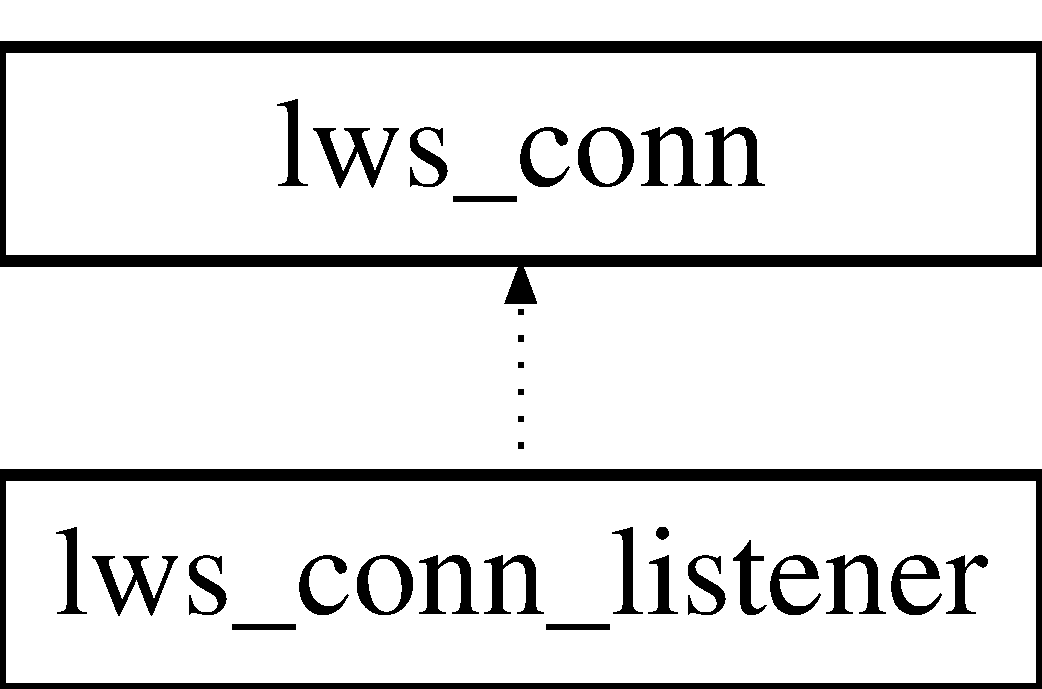
\includegraphics[height=2.000000cm]{classlws__conn}
\end{center}
\end{figure}
\subsection*{Public Member Functions}
\begin{DoxyCompactItemize}
\item 
void {\bfseries set\+\_\+wsi} (struct lws $\ast$\+\_\+wsi)\hypertarget{classlws__conn_afe73e53da2070f659ad6e7fd14878c7e}{}\label{classlws__conn_afe73e53da2070f659ad6e7fd14878c7e}

\item 
int {\bfseries actual\+\_\+on\+RX} (Socket $\ast$s)\hypertarget{classlws__conn_aef530971372f55e862f2e09bc98f1029}{}\label{classlws__conn_aef530971372f55e862f2e09bc98f1029}

\item 
void {\bfseries on\+RX} (Socket $\ast$s)\hypertarget{classlws__conn_aba42bdd763a36c3a331b62410969b6ba}{}\label{classlws__conn_aba42bdd763a36c3a331b62410969b6ba}

\item 
void {\bfseries on\+Error} (Socket $\ast$s, socket\+\_\+error\+\_\+t err)\hypertarget{classlws__conn_a4fb477fad697ce1faf8ec7a884ea6c6b}{}\label{classlws__conn_a4fb477fad697ce1faf8ec7a884ea6c6b}

\item 
void {\bfseries on\+Disconnect} (T\+C\+P\+Stream $\ast$s)\hypertarget{classlws__conn_a49f87612c6a3098cd1587f8382b8c85b}{}\label{classlws__conn_a49f87612c6a3098cd1587f8382b8c85b}

\item 
void {\bfseries on\+Sent} (Socket $\ast$s, uint16\+\_\+t len)\hypertarget{classlws__conn_aad7d2406618e560114650a91c729a596}{}\label{classlws__conn_aad7d2406618e560114650a91c729a596}

\item 
void {\bfseries serialized\+\_\+writeable} (struct lws $\ast$wsi)\hypertarget{classlws__conn_accc57581269c554291dac840ed135231}{}\label{classlws__conn_accc57581269c554291dac840ed135231}

\end{DoxyCompactItemize}
\subsection*{Data Fields}
\begin{DoxyCompactItemize}
\item 
T\+C\+P\+Stream $\ast$ {\bfseries ts}\hypertarget{classlws__conn_a5cad031b6b779da42b37f4007cae541b}{}\label{classlws__conn_a5cad031b6b779da42b37f4007cae541b}

\item 
struct lws $\ast$ {\bfseries wsi}\hypertarget{classlws__conn_a7e504bd449ffb51c7ab1d2126613ebc3}{}\label{classlws__conn_a7e504bd449ffb51c7ab1d2126613ebc3}

\item 
char {\bfseries writeable}\hypertarget{classlws__conn_a8e1fdd467b7f66fc438dc70ae979b938}{}\label{classlws__conn_a8e1fdd467b7f66fc438dc70ae979b938}

\item 
char {\bfseries awaiting\+\_\+on\+\_\+writeable}\hypertarget{classlws__conn_a5226010afdf5421f279454e5cbb282a4}{}\label{classlws__conn_a5226010afdf5421f279454e5cbb282a4}

\end{DoxyCompactItemize}


The documentation for this class was generated from the following file\+:\begin{DoxyCompactItemize}
\item 
lib/\hyperlink{libwebsockets_8h}{libwebsockets.\+h}\end{DoxyCompactItemize}

\hypertarget{classlws__conn__listener}{}\section{lws\+\_\+conn\+\_\+listener Class Reference}
\label{classlws__conn__listener}\index{lws\+\_\+conn\+\_\+listener@{lws\+\_\+conn\+\_\+listener}}
Inheritance diagram for lws\+\_\+conn\+\_\+listener\+:\begin{figure}[H]
\begin{center}
\leavevmode
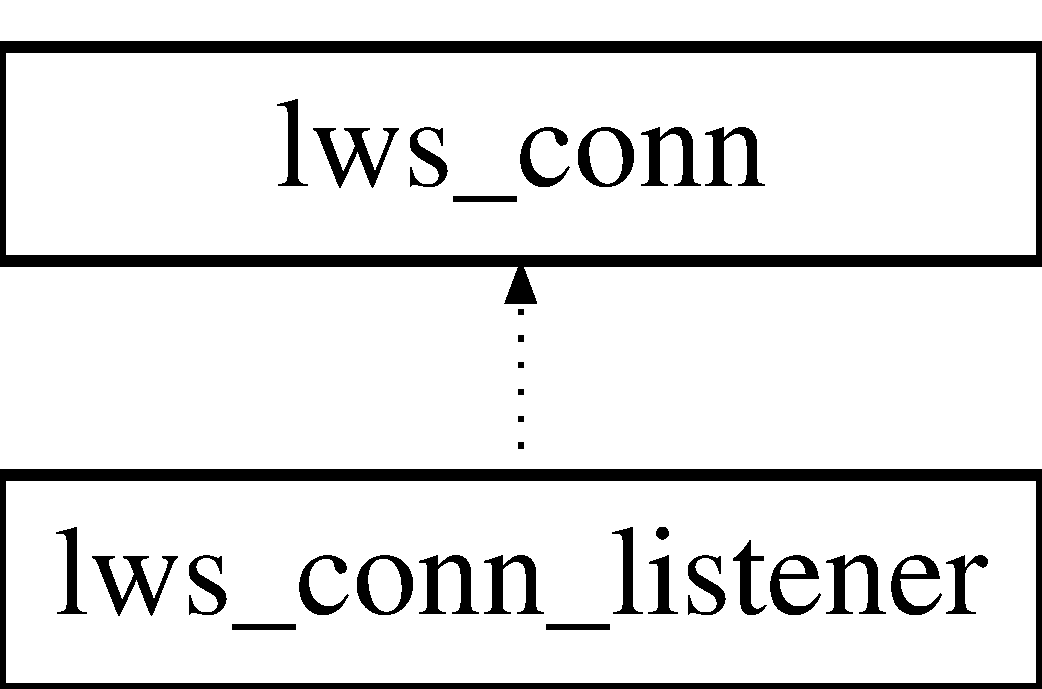
\includegraphics[height=2.000000cm]{classlws__conn__listener}
\end{center}
\end{figure}
\subsection*{Public Member Functions}
\begin{DoxyCompactItemize}
\item 
void \hyperlink{classlws__conn__listener_a3c19c314f2ea2b758407b4041e4c4010}{start} (const uint16\+\_\+t port)
\end{DoxyCompactItemize}
\subsection*{Data Fields}
\begin{DoxyCompactItemize}
\item 
T\+C\+P\+Listener {\bfseries srv}\hypertarget{classlws__conn__listener_aa7076f8965bb9df268798fd9a0283374}{}\label{classlws__conn__listener_aa7076f8965bb9df268798fd9a0283374}

\end{DoxyCompactItemize}
\subsection*{Protected Member Functions}
\begin{DoxyCompactItemize}
\item 
void \hyperlink{classlws__conn__listener_ab3bc839797ba14554ac70ad09fd155c7}{on\+RX} (Socket $\ast$s)
\item 
void \hyperlink{classlws__conn__listener_a271ac4f8ad5770b3bc96cce5b265b72c}{on\+Error} (Socket $\ast$s, socket\+\_\+error\+\_\+t err)
\item 
void \hyperlink{classlws__conn__listener_ab432a456c3a961ec562e06141897806b}{on\+Incoming} (T\+C\+P\+Listener $\ast$s, void $\ast$impl)
\item 
void \hyperlink{classlws__conn__listener_aab3c7bf550a8f15d20f1e093125c2e60}{on\+Disconnect} (T\+C\+P\+Stream $\ast$s)
\end{DoxyCompactItemize}


\subsection{Member Function Documentation}
\index{lws\+\_\+conn\+\_\+listener@{lws\+\_\+conn\+\_\+listener}!on\+Disconnect@{on\+Disconnect}}
\index{on\+Disconnect@{on\+Disconnect}!lws\+\_\+conn\+\_\+listener@{lws\+\_\+conn\+\_\+listener}}
\subsubsection[{\texorpdfstring{on\+Disconnect(\+T\+C\+P\+Stream $\ast$s)}{onDisconnect(TCPStream *s)}}]{\setlength{\rightskip}{0pt plus 5cm}void lws\+\_\+conn\+\_\+listener\+::on\+Disconnect (
\begin{DoxyParamCaption}
\item[{T\+C\+P\+Stream $\ast$}]{s}
\end{DoxyParamCaption}
)\hspace{0.3cm}{\ttfamily [protected]}}\hypertarget{classlws__conn__listener_aab3c7bf550a8f15d20f1e093125c2e60}{}\label{classlws__conn__listener_aab3c7bf550a8f15d20f1e093125c2e60}
disconnection \index{lws\+\_\+conn\+\_\+listener@{lws\+\_\+conn\+\_\+listener}!on\+Error@{on\+Error}}
\index{on\+Error@{on\+Error}!lws\+\_\+conn\+\_\+listener@{lws\+\_\+conn\+\_\+listener}}
\subsubsection[{\texorpdfstring{on\+Error(\+Socket $\ast$s, socket\+\_\+error\+\_\+t err)}{onError(Socket *s, socket\_error\_t err)}}]{\setlength{\rightskip}{0pt plus 5cm}void lws\+\_\+conn\+\_\+listener\+::on\+Error (
\begin{DoxyParamCaption}
\item[{Socket $\ast$}]{s, }
\item[{socket\+\_\+error\+\_\+t}]{err}
\end{DoxyParamCaption}
)\hspace{0.3cm}{\ttfamily [protected]}}\hypertarget{classlws__conn__listener_a271ac4f8ad5770b3bc96cce5b265b72c}{}\label{classlws__conn__listener_a271ac4f8ad5770b3bc96cce5b265b72c}
if error occurs \index{lws\+\_\+conn\+\_\+listener@{lws\+\_\+conn\+\_\+listener}!on\+Incoming@{on\+Incoming}}
\index{on\+Incoming@{on\+Incoming}!lws\+\_\+conn\+\_\+listener@{lws\+\_\+conn\+\_\+listener}}
\subsubsection[{\texorpdfstring{on\+Incoming(\+T\+C\+P\+Listener $\ast$s, void $\ast$impl)}{onIncoming(TCPListener *s, void *impl)}}]{\setlength{\rightskip}{0pt plus 5cm}void lws\+\_\+conn\+\_\+listener\+::on\+Incoming (
\begin{DoxyParamCaption}
\item[{T\+C\+P\+Listener $\ast$}]{s, }
\item[{void $\ast$}]{impl}
\end{DoxyParamCaption}
)\hspace{0.3cm}{\ttfamily [protected]}}\hypertarget{classlws__conn__listener_ab432a456c3a961ec562e06141897806b}{}\label{classlws__conn__listener_ab432a456c3a961ec562e06141897806b}
new connection \index{lws\+\_\+conn\+\_\+listener@{lws\+\_\+conn\+\_\+listener}!on\+RX@{on\+RX}}
\index{on\+RX@{on\+RX}!lws\+\_\+conn\+\_\+listener@{lws\+\_\+conn\+\_\+listener}}
\subsubsection[{\texorpdfstring{on\+R\+X(\+Socket $\ast$s)}{onRX(Socket *s)}}]{\setlength{\rightskip}{0pt plus 5cm}void lws\+\_\+conn\+\_\+listener\+::on\+RX (
\begin{DoxyParamCaption}
\item[{Socket $\ast$}]{s}
\end{DoxyParamCaption}
)\hspace{0.3cm}{\ttfamily [protected]}}\hypertarget{classlws__conn__listener_ab3bc839797ba14554ac70ad09fd155c7}{}\label{classlws__conn__listener_ab3bc839797ba14554ac70ad09fd155c7}
incoming data ready \index{lws\+\_\+conn\+\_\+listener@{lws\+\_\+conn\+\_\+listener}!start@{start}}
\index{start@{start}!lws\+\_\+conn\+\_\+listener@{lws\+\_\+conn\+\_\+listener}}
\subsubsection[{\texorpdfstring{start(const uint16\+\_\+t port)}{start(const uint16\_t port)}}]{\setlength{\rightskip}{0pt plus 5cm}void lws\+\_\+conn\+\_\+listener\+::start (
\begin{DoxyParamCaption}
\item[{const uint16\+\_\+t}]{port}
\end{DoxyParamCaption}
)}\hypertarget{classlws__conn__listener_a3c19c314f2ea2b758407b4041e4c4010}{}\label{classlws__conn__listener_a3c19c314f2ea2b758407b4041e4c4010}
start listening 

The documentation for this class was generated from the following file\+:\begin{DoxyCompactItemize}
\item 
lib/\hyperlink{libwebsockets_8h}{libwebsockets.\+h}\end{DoxyCompactItemize}

\hypertarget{structlws__context__creation__info}{}\section{lws\+\_\+context\+\_\+creation\+\_\+info Struct Reference}
\label{structlws__context__creation__info}\index{lws\+\_\+context\+\_\+creation\+\_\+info@{lws\+\_\+context\+\_\+creation\+\_\+info}}


{\ttfamily \#include $<$libwebsockets.\+h$>$}

\subsection*{Data Fields}
\begin{DoxyCompactItemize}
\item 
int \hyperlink{structlws__context__creation__info_a424a5ce268d6903e42243be94487ab85}{port}
\item 
const char $\ast$ \hyperlink{structlws__context__creation__info_a75434932bb5df54665ea678eb8ac104a}{iface}
\item 
const struct \hyperlink{structlws__protocols}{lws\+\_\+protocols} $\ast$ \hyperlink{structlws__context__creation__info_abb90ffb3e6d6db2db20f529d61bd9122}{protocols}
\item 
const struct \hyperlink{structlws__extension}{lws\+\_\+extension} $\ast$ \hyperlink{structlws__context__creation__info_a4a3d1155fc52f5048b481884f6fb947c}{extensions}
\item 
const struct \hyperlink{structlws__token__limits}{lws\+\_\+token\+\_\+limits} $\ast$ \hyperlink{structlws__context__creation__info_ac8a75b7b259a3c3a5fbb4219a3f06c29}{token\+\_\+limits}
\item 
const char $\ast$ \hyperlink{structlws__context__creation__info_af3fb447be15c4fcb01d3285a6678ab54}{ssl\+\_\+private\+\_\+key\+\_\+password}
\item 
const char $\ast$ \hyperlink{structlws__context__creation__info_ac62b0f0e8e402412ba5011d15c244103}{ssl\+\_\+cert\+\_\+filepath}
\item 
const char $\ast$ \hyperlink{structlws__context__creation__info_ab9ec8893e0f7843cf5d783d2f350ef14}{ssl\+\_\+private\+\_\+key\+\_\+filepath}
\item 
const char $\ast$ \hyperlink{structlws__context__creation__info_a4f8e65c3a059d3b586fafa9ef3282c29}{ssl\+\_\+ca\+\_\+filepath}
\item 
const char $\ast$ \hyperlink{structlws__context__creation__info_a3e1516fd7fed26bfa77c0246ed26c2eb}{ssl\+\_\+cipher\+\_\+list}
\item 
const char $\ast$ \hyperlink{structlws__context__creation__info_aef917c0b23976a264d2474901b4f5aa3}{http\+\_\+proxy\+\_\+address}
\item 
unsigned int \hyperlink{structlws__context__creation__info_a7b59f2bdc869871e7bde232db94f5ca6}{http\+\_\+proxy\+\_\+port}
\item 
int \hyperlink{structlws__context__creation__info_a9c9d22437de92c197f3cee52912b2c03}{gid}
\item 
int \hyperlink{structlws__context__creation__info_ac105b4180008cb3e672d57beead8382e}{uid}
\item 
unsigned int \hyperlink{structlws__context__creation__info_a9d3b17a25e1fbc772f21eb4959a82724}{options}
\item 
void $\ast$ \hyperlink{structlws__context__creation__info_a0e9d94cdfb893d777b4a4db81e7b5ac0}{user}
\item 
int \hyperlink{structlws__context__creation__info_ac583ce92b8e1c949cb6fef6bfe713d56}{ka\+\_\+time}
\item 
int \hyperlink{structlws__context__creation__info_a3baab4285c679fbe027c2504621d7410}{ka\+\_\+probes}
\item 
int \hyperlink{structlws__context__creation__info_a381342a398883d6204955ff3c1849ddd}{ka\+\_\+interval}
\item 
\hyperlink{structlws__polarssl__context}{S\+S\+L\+\_\+\+C\+TX} $\ast$ \hyperlink{structlws__context__creation__info_a1654d41bea6fb2f619b57e6a264b26a4}{provided\+\_\+client\+\_\+ssl\+\_\+ctx}
\item 
void $\ast$ \hyperlink{structlws__context__creation__info_a0e790dda6202604f73a03b6149bc12bb}{provided\+\_\+client\+\_\+ssl\+\_\+ctx}
\item 
short \hyperlink{structlws__context__creation__info_a0cdfd3c484689ba6f0f2cc91b38ce948}{max\+\_\+http\+\_\+header\+\_\+data}
\item 
short \hyperlink{structlws__context__creation__info_a0b154e79abc1167ba4ac3539f4af6720}{max\+\_\+http\+\_\+header\+\_\+pool}
\item 
unsigned int \hyperlink{structlws__context__creation__info_ae52f3237e144e9ddcab5e2cf91d1e419}{count\+\_\+threads}
\item 
unsigned int \hyperlink{structlws__context__creation__info_a45e63e24c88289e0c8352377ef4d3646}{fd\+\_\+limit\+\_\+per\+\_\+thread}
\item 
unsigned int \hyperlink{structlws__context__creation__info_a6cfa3d51df2def3349a5cbf0d712822d}{timeout\+\_\+secs}
\item 
const char $\ast$ \hyperlink{structlws__context__creation__info_afa5d4e7d9f86b58a1c6fac14f0a5f5f9}{ecdh\+\_\+curve}
\item 
const char $\ast$ \hyperlink{structlws__context__creation__info_ad50db098a208f045f7811207d2bee4b9}{vhost\+\_\+name}
\item 
const char $\ast$const $\ast$ \hyperlink{structlws__context__creation__info_a8122cfc0810bafe51edb3ba6bf9a1251}{plugin\+\_\+dirs}
\item 
const struct \hyperlink{structlws__protocol__vhost__options}{lws\+\_\+protocol\+\_\+vhost\+\_\+options} $\ast$ \hyperlink{structlws__context__creation__info_a999866fcd15dbd621773436f97190458}{pvo}
\item 
int \hyperlink{structlws__context__creation__info_a81697c6b763b5ef3ee52862bc70b07d6}{keepalive\+\_\+timeout}
\item 
const char $\ast$ \hyperlink{structlws__context__creation__info_ad0e95ba721f7bd2b676719f8093c23a2}{log\+\_\+filepath}
\item 
const struct \hyperlink{structlws__http__mount}{lws\+\_\+http\+\_\+mount} $\ast$ \hyperlink{structlws__context__creation__info_a13ffbb0d010309669611f8c4eda7d7f8}{mounts}
\item 
const char $\ast$ \hyperlink{structlws__context__creation__info_a137a9b9de4f6a7993fed8746d551e616}{server\+\_\+string}
\item 
unsigned int \hyperlink{structlws__context__creation__info_a57f88c0745adbd1d6b9b619b8de30209}{pt\+\_\+serv\+\_\+buf\+\_\+size}
\item 
unsigned int \hyperlink{structlws__context__creation__info_aa8d9e85e137f35fb006f2e4a53f0887a}{max\+\_\+http\+\_\+header\+\_\+data2}
\item 
long \hyperlink{structlws__context__creation__info_a704940261951ced6b5d8191bd8b9bb2d}{ssl\+\_\+options\+\_\+set}
\item 
long \hyperlink{structlws__context__creation__info_adb0bc0b28cd7d90ab306723d8ffa96fa}{ssl\+\_\+options\+\_\+clear}
\item 
void $\ast$ \hyperlink{structlws__context__creation__info_afce3b59950eca3203faa07381bbed5d7}{\+\_\+unused} \mbox{[}8\mbox{]}
\end{DoxyCompactItemize}


\subsection{Detailed Description}
struct \hyperlink{structlws__context__creation__info}{lws\+\_\+context\+\_\+creation\+\_\+info} -\/ parameters to create context and /or vhost with

This is also used to create vhosts.... if L\+W\+S\+\_\+\+S\+E\+R\+V\+E\+R\+\_\+\+O\+P\+T\+I\+O\+N\+\_\+\+E\+X\+P\+L\+I\+C\+I\+T\+\_\+\+V\+H\+O\+S\+TS is not given, then for backwards compatibility one vhost is created at context-\/creation time using the info from this struct.

If L\+W\+S\+\_\+\+S\+E\+R\+V\+E\+R\+\_\+\+O\+P\+T\+I\+O\+N\+\_\+\+E\+X\+P\+L\+I\+C\+I\+T\+\_\+\+V\+H\+O\+S\+TS is given, then no vhosts are created at the same time as the context, they are expected to be created afterwards. 

\subsection{Field Documentation}
\index{lws\+\_\+context\+\_\+creation\+\_\+info@{lws\+\_\+context\+\_\+creation\+\_\+info}!\+\_\+unused@{\+\_\+unused}}
\index{\+\_\+unused@{\+\_\+unused}!lws\+\_\+context\+\_\+creation\+\_\+info@{lws\+\_\+context\+\_\+creation\+\_\+info}}
\subsubsection[{\texorpdfstring{\+\_\+unused}{\_unused}}]{\setlength{\rightskip}{0pt plus 5cm}void$\ast$ lws\+\_\+context\+\_\+creation\+\_\+info\+::\+\_\+unused\mbox{[}8\mbox{]}}\hypertarget{structlws__context__creation__info_afce3b59950eca3203faa07381bbed5d7}{}\label{structlws__context__creation__info_afce3b59950eca3203faa07381bbed5d7}
dummy \index{lws\+\_\+context\+\_\+creation\+\_\+info@{lws\+\_\+context\+\_\+creation\+\_\+info}!count\+\_\+threads@{count\+\_\+threads}}
\index{count\+\_\+threads@{count\+\_\+threads}!lws\+\_\+context\+\_\+creation\+\_\+info@{lws\+\_\+context\+\_\+creation\+\_\+info}}
\subsubsection[{\texorpdfstring{count\+\_\+threads}{count\_threads}}]{\setlength{\rightskip}{0pt plus 5cm}unsigned int lws\+\_\+context\+\_\+creation\+\_\+info\+::count\+\_\+threads}\hypertarget{structlws__context__creation__info_ae52f3237e144e9ddcab5e2cf91d1e419}{}\label{structlws__context__creation__info_ae52f3237e144e9ddcab5e2cf91d1e419}
C\+O\+N\+T\+E\+XT\+: how many contexts to create in an array, 0 = 1 \index{lws\+\_\+context\+\_\+creation\+\_\+info@{lws\+\_\+context\+\_\+creation\+\_\+info}!ecdh\+\_\+curve@{ecdh\+\_\+curve}}
\index{ecdh\+\_\+curve@{ecdh\+\_\+curve}!lws\+\_\+context\+\_\+creation\+\_\+info@{lws\+\_\+context\+\_\+creation\+\_\+info}}
\subsubsection[{\texorpdfstring{ecdh\+\_\+curve}{ecdh\_curve}}]{\setlength{\rightskip}{0pt plus 5cm}const char$\ast$ lws\+\_\+context\+\_\+creation\+\_\+info\+::ecdh\+\_\+curve}\hypertarget{structlws__context__creation__info_afa5d4e7d9f86b58a1c6fac14f0a5f5f9}{}\label{structlws__context__creation__info_afa5d4e7d9f86b58a1c6fac14f0a5f5f9}
V\+H\+O\+ST\+: if N\+U\+LL, defaults to initializing server with \char`\"{}prime256v1\char`\"{} \index{lws\+\_\+context\+\_\+creation\+\_\+info@{lws\+\_\+context\+\_\+creation\+\_\+info}!extensions@{extensions}}
\index{extensions@{extensions}!lws\+\_\+context\+\_\+creation\+\_\+info@{lws\+\_\+context\+\_\+creation\+\_\+info}}
\subsubsection[{\texorpdfstring{extensions}{extensions}}]{\setlength{\rightskip}{0pt plus 5cm}const struct {\bf lws\+\_\+extension}$\ast$ lws\+\_\+context\+\_\+creation\+\_\+info\+::extensions}\hypertarget{structlws__context__creation__info_a4a3d1155fc52f5048b481884f6fb947c}{}\label{structlws__context__creation__info_a4a3d1155fc52f5048b481884f6fb947c}
V\+H\+O\+ST\+: N\+U\+LL or array of \hyperlink{structlws__extension}{lws\+\_\+extension} structs listing the extensions this context supports. \index{lws\+\_\+context\+\_\+creation\+\_\+info@{lws\+\_\+context\+\_\+creation\+\_\+info}!fd\+\_\+limit\+\_\+per\+\_\+thread@{fd\+\_\+limit\+\_\+per\+\_\+thread}}
\index{fd\+\_\+limit\+\_\+per\+\_\+thread@{fd\+\_\+limit\+\_\+per\+\_\+thread}!lws\+\_\+context\+\_\+creation\+\_\+info@{lws\+\_\+context\+\_\+creation\+\_\+info}}
\subsubsection[{\texorpdfstring{fd\+\_\+limit\+\_\+per\+\_\+thread}{fd\_limit\_per\_thread}}]{\setlength{\rightskip}{0pt plus 5cm}unsigned int lws\+\_\+context\+\_\+creation\+\_\+info\+::fd\+\_\+limit\+\_\+per\+\_\+thread}\hypertarget{structlws__context__creation__info_a45e63e24c88289e0c8352377ef4d3646}{}\label{structlws__context__creation__info_a45e63e24c88289e0c8352377ef4d3646}
C\+O\+N\+T\+E\+XT\+: nonzero means restrict each service thread to this many fds, 0 means the default which is divide the process fd limit by the number of threads. \index{lws\+\_\+context\+\_\+creation\+\_\+info@{lws\+\_\+context\+\_\+creation\+\_\+info}!gid@{gid}}
\index{gid@{gid}!lws\+\_\+context\+\_\+creation\+\_\+info@{lws\+\_\+context\+\_\+creation\+\_\+info}}
\subsubsection[{\texorpdfstring{gid}{gid}}]{\setlength{\rightskip}{0pt plus 5cm}int lws\+\_\+context\+\_\+creation\+\_\+info\+::gid}\hypertarget{structlws__context__creation__info_a9c9d22437de92c197f3cee52912b2c03}{}\label{structlws__context__creation__info_a9c9d22437de92c197f3cee52912b2c03}
C\+O\+N\+T\+E\+XT\+: group id to change to after setting listen socket, or -\/1. \index{lws\+\_\+context\+\_\+creation\+\_\+info@{lws\+\_\+context\+\_\+creation\+\_\+info}!http\+\_\+proxy\+\_\+address@{http\+\_\+proxy\+\_\+address}}
\index{http\+\_\+proxy\+\_\+address@{http\+\_\+proxy\+\_\+address}!lws\+\_\+context\+\_\+creation\+\_\+info@{lws\+\_\+context\+\_\+creation\+\_\+info}}
\subsubsection[{\texorpdfstring{http\+\_\+proxy\+\_\+address}{http\_proxy\_address}}]{\setlength{\rightskip}{0pt plus 5cm}const char$\ast$ lws\+\_\+context\+\_\+creation\+\_\+info\+::http\+\_\+proxy\+\_\+address}\hypertarget{structlws__context__creation__info_aef917c0b23976a264d2474901b4f5aa3}{}\label{structlws__context__creation__info_aef917c0b23976a264d2474901b4f5aa3}
V\+H\+O\+ST\+: If non-\/\+N\+U\+LL, attempts to proxy via the given address. If proxy auth is required, use format \char`\"{}username\+:password\textbackslash{}@server\+:port\char`\"{} \index{lws\+\_\+context\+\_\+creation\+\_\+info@{lws\+\_\+context\+\_\+creation\+\_\+info}!http\+\_\+proxy\+\_\+port@{http\+\_\+proxy\+\_\+port}}
\index{http\+\_\+proxy\+\_\+port@{http\+\_\+proxy\+\_\+port}!lws\+\_\+context\+\_\+creation\+\_\+info@{lws\+\_\+context\+\_\+creation\+\_\+info}}
\subsubsection[{\texorpdfstring{http\+\_\+proxy\+\_\+port}{http\_proxy\_port}}]{\setlength{\rightskip}{0pt plus 5cm}unsigned int lws\+\_\+context\+\_\+creation\+\_\+info\+::http\+\_\+proxy\+\_\+port}\hypertarget{structlws__context__creation__info_a7b59f2bdc869871e7bde232db94f5ca6}{}\label{structlws__context__creation__info_a7b59f2bdc869871e7bde232db94f5ca6}
V\+H\+O\+ST\+: If http\+\_\+proxy\+\_\+address was non-\/\+N\+U\+LL, uses this port \index{lws\+\_\+context\+\_\+creation\+\_\+info@{lws\+\_\+context\+\_\+creation\+\_\+info}!iface@{iface}}
\index{iface@{iface}!lws\+\_\+context\+\_\+creation\+\_\+info@{lws\+\_\+context\+\_\+creation\+\_\+info}}
\subsubsection[{\texorpdfstring{iface}{iface}}]{\setlength{\rightskip}{0pt plus 5cm}const char$\ast$ lws\+\_\+context\+\_\+creation\+\_\+info\+::iface}\hypertarget{structlws__context__creation__info_a75434932bb5df54665ea678eb8ac104a}{}\label{structlws__context__creation__info_a75434932bb5df54665ea678eb8ac104a}
V\+H\+O\+ST\+: N\+U\+LL to bind the listen socket to all interfaces, or the interface name, eg, \char`\"{}eth2\char`\"{} If options specifies L\+W\+S\+\_\+\+S\+E\+R\+V\+E\+R\+\_\+\+O\+P\+T\+I\+O\+N\+\_\+\+U\+N\+I\+X\+\_\+\+S\+O\+CK, this member is the pathname of a U\+N\+IX domain socket. you can use the U\+N\+IX domain sockets in abstract namespace, by prepending an at symbol to the socket name. \index{lws\+\_\+context\+\_\+creation\+\_\+info@{lws\+\_\+context\+\_\+creation\+\_\+info}!ka\+\_\+interval@{ka\+\_\+interval}}
\index{ka\+\_\+interval@{ka\+\_\+interval}!lws\+\_\+context\+\_\+creation\+\_\+info@{lws\+\_\+context\+\_\+creation\+\_\+info}}
\subsubsection[{\texorpdfstring{ka\+\_\+interval}{ka\_interval}}]{\setlength{\rightskip}{0pt plus 5cm}int lws\+\_\+context\+\_\+creation\+\_\+info\+::ka\+\_\+interval}\hypertarget{structlws__context__creation__info_a381342a398883d6204955ff3c1849ddd}{}\label{structlws__context__creation__info_a381342a398883d6204955ff3c1849ddd}
C\+O\+N\+T\+E\+XT\+: if ka\+\_\+time was nonzero, how long to wait before each ka\+\_\+probes attempt \index{lws\+\_\+context\+\_\+creation\+\_\+info@{lws\+\_\+context\+\_\+creation\+\_\+info}!ka\+\_\+probes@{ka\+\_\+probes}}
\index{ka\+\_\+probes@{ka\+\_\+probes}!lws\+\_\+context\+\_\+creation\+\_\+info@{lws\+\_\+context\+\_\+creation\+\_\+info}}
\subsubsection[{\texorpdfstring{ka\+\_\+probes}{ka\_probes}}]{\setlength{\rightskip}{0pt plus 5cm}int lws\+\_\+context\+\_\+creation\+\_\+info\+::ka\+\_\+probes}\hypertarget{structlws__context__creation__info_a3baab4285c679fbe027c2504621d7410}{}\label{structlws__context__creation__info_a3baab4285c679fbe027c2504621d7410}
C\+O\+N\+T\+E\+XT\+: if ka\+\_\+time was nonzero, after the timeout expires how many times to try to get a response from the peer before giving up and killing the connection \index{lws\+\_\+context\+\_\+creation\+\_\+info@{lws\+\_\+context\+\_\+creation\+\_\+info}!ka\+\_\+time@{ka\+\_\+time}}
\index{ka\+\_\+time@{ka\+\_\+time}!lws\+\_\+context\+\_\+creation\+\_\+info@{lws\+\_\+context\+\_\+creation\+\_\+info}}
\subsubsection[{\texorpdfstring{ka\+\_\+time}{ka\_time}}]{\setlength{\rightskip}{0pt plus 5cm}int lws\+\_\+context\+\_\+creation\+\_\+info\+::ka\+\_\+time}\hypertarget{structlws__context__creation__info_ac583ce92b8e1c949cb6fef6bfe713d56}{}\label{structlws__context__creation__info_ac583ce92b8e1c949cb6fef6bfe713d56}
C\+O\+N\+T\+E\+XT\+: 0 for no T\+CP keepalive, otherwise apply this keepalive timeout to all libwebsocket sockets, client or server \index{lws\+\_\+context\+\_\+creation\+\_\+info@{lws\+\_\+context\+\_\+creation\+\_\+info}!keepalive\+\_\+timeout@{keepalive\+\_\+timeout}}
\index{keepalive\+\_\+timeout@{keepalive\+\_\+timeout}!lws\+\_\+context\+\_\+creation\+\_\+info@{lws\+\_\+context\+\_\+creation\+\_\+info}}
\subsubsection[{\texorpdfstring{keepalive\+\_\+timeout}{keepalive\_timeout}}]{\setlength{\rightskip}{0pt plus 5cm}int lws\+\_\+context\+\_\+creation\+\_\+info\+::keepalive\+\_\+timeout}\hypertarget{structlws__context__creation__info_a81697c6b763b5ef3ee52862bc70b07d6}{}\label{structlws__context__creation__info_a81697c6b763b5ef3ee52862bc70b07d6}
V\+H\+O\+ST\+: (default = 0 = 60s) seconds to allow remote client to hold on to an idle H\+T\+T\+P/1.\+1 connection \index{lws\+\_\+context\+\_\+creation\+\_\+info@{lws\+\_\+context\+\_\+creation\+\_\+info}!log\+\_\+filepath@{log\+\_\+filepath}}
\index{log\+\_\+filepath@{log\+\_\+filepath}!lws\+\_\+context\+\_\+creation\+\_\+info@{lws\+\_\+context\+\_\+creation\+\_\+info}}
\subsubsection[{\texorpdfstring{log\+\_\+filepath}{log\_filepath}}]{\setlength{\rightskip}{0pt plus 5cm}const char$\ast$ lws\+\_\+context\+\_\+creation\+\_\+info\+::log\+\_\+filepath}\hypertarget{structlws__context__creation__info_ad0e95ba721f7bd2b676719f8093c23a2}{}\label{structlws__context__creation__info_ad0e95ba721f7bd2b676719f8093c23a2}
V\+H\+O\+ST\+: filepath to append logs to... this is opened before any dropping of initial privileges \index{lws\+\_\+context\+\_\+creation\+\_\+info@{lws\+\_\+context\+\_\+creation\+\_\+info}!max\+\_\+http\+\_\+header\+\_\+data@{max\+\_\+http\+\_\+header\+\_\+data}}
\index{max\+\_\+http\+\_\+header\+\_\+data@{max\+\_\+http\+\_\+header\+\_\+data}!lws\+\_\+context\+\_\+creation\+\_\+info@{lws\+\_\+context\+\_\+creation\+\_\+info}}
\subsubsection[{\texorpdfstring{max\+\_\+http\+\_\+header\+\_\+data}{max\_http\_header\_data}}]{\setlength{\rightskip}{0pt plus 5cm}short lws\+\_\+context\+\_\+creation\+\_\+info\+::max\+\_\+http\+\_\+header\+\_\+data}\hypertarget{structlws__context__creation__info_a0cdfd3c484689ba6f0f2cc91b38ce948}{}\label{structlws__context__creation__info_a0cdfd3c484689ba6f0f2cc91b38ce948}
C\+O\+N\+T\+E\+XT\+: The max amount of header payload that can be handled in an http request (unrecognized header payload is dropped) \index{lws\+\_\+context\+\_\+creation\+\_\+info@{lws\+\_\+context\+\_\+creation\+\_\+info}!max\+\_\+http\+\_\+header\+\_\+data2@{max\+\_\+http\+\_\+header\+\_\+data2}}
\index{max\+\_\+http\+\_\+header\+\_\+data2@{max\+\_\+http\+\_\+header\+\_\+data2}!lws\+\_\+context\+\_\+creation\+\_\+info@{lws\+\_\+context\+\_\+creation\+\_\+info}}
\subsubsection[{\texorpdfstring{max\+\_\+http\+\_\+header\+\_\+data2}{max\_http\_header\_data2}}]{\setlength{\rightskip}{0pt plus 5cm}unsigned int lws\+\_\+context\+\_\+creation\+\_\+info\+::max\+\_\+http\+\_\+header\+\_\+data2}\hypertarget{structlws__context__creation__info_aa8d9e85e137f35fb006f2e4a53f0887a}{}\label{structlws__context__creation__info_aa8d9e85e137f35fb006f2e4a53f0887a}
C\+O\+N\+T\+E\+XT\+: if max\+\_\+http\+\_\+header\+\_\+data is 0 and this is nonzero, this will be used in place of the default. It\textquotesingle{}s like this for compatibility with the original short version, this is unsigned int length. \index{lws\+\_\+context\+\_\+creation\+\_\+info@{lws\+\_\+context\+\_\+creation\+\_\+info}!max\+\_\+http\+\_\+header\+\_\+pool@{max\+\_\+http\+\_\+header\+\_\+pool}}
\index{max\+\_\+http\+\_\+header\+\_\+pool@{max\+\_\+http\+\_\+header\+\_\+pool}!lws\+\_\+context\+\_\+creation\+\_\+info@{lws\+\_\+context\+\_\+creation\+\_\+info}}
\subsubsection[{\texorpdfstring{max\+\_\+http\+\_\+header\+\_\+pool}{max\_http\_header\_pool}}]{\setlength{\rightskip}{0pt plus 5cm}short lws\+\_\+context\+\_\+creation\+\_\+info\+::max\+\_\+http\+\_\+header\+\_\+pool}\hypertarget{structlws__context__creation__info_a0b154e79abc1167ba4ac3539f4af6720}{}\label{structlws__context__creation__info_a0b154e79abc1167ba4ac3539f4af6720}
C\+O\+N\+T\+E\+XT\+: The max number of connections with http headers that can be processed simultaneously (the corresponding memory is allocated for the lifetime of the context). If the pool is busy new incoming connections must wait for accept until one becomes free. \index{lws\+\_\+context\+\_\+creation\+\_\+info@{lws\+\_\+context\+\_\+creation\+\_\+info}!mounts@{mounts}}
\index{mounts@{mounts}!lws\+\_\+context\+\_\+creation\+\_\+info@{lws\+\_\+context\+\_\+creation\+\_\+info}}
\subsubsection[{\texorpdfstring{mounts}{mounts}}]{\setlength{\rightskip}{0pt plus 5cm}const struct {\bf lws\+\_\+http\+\_\+mount}$\ast$ lws\+\_\+context\+\_\+creation\+\_\+info\+::mounts}\hypertarget{structlws__context__creation__info_a13ffbb0d010309669611f8c4eda7d7f8}{}\label{structlws__context__creation__info_a13ffbb0d010309669611f8c4eda7d7f8}
V\+H\+O\+ST\+: optional linked list of mounts for this vhost \index{lws\+\_\+context\+\_\+creation\+\_\+info@{lws\+\_\+context\+\_\+creation\+\_\+info}!options@{options}}
\index{options@{options}!lws\+\_\+context\+\_\+creation\+\_\+info@{lws\+\_\+context\+\_\+creation\+\_\+info}}
\subsubsection[{\texorpdfstring{options}{options}}]{\setlength{\rightskip}{0pt plus 5cm}unsigned int lws\+\_\+context\+\_\+creation\+\_\+info\+::options}\hypertarget{structlws__context__creation__info_a9d3b17a25e1fbc772f21eb4959a82724}{}\label{structlws__context__creation__info_a9d3b17a25e1fbc772f21eb4959a82724}
V\+H\+O\+ST + C\+O\+N\+T\+E\+XT\+: 0, or L\+W\+S\+\_\+\+S\+E\+R\+V\+E\+R\+\_\+\+O\+P\+T\+I\+O\+N\+\_\+... bitfields \index{lws\+\_\+context\+\_\+creation\+\_\+info@{lws\+\_\+context\+\_\+creation\+\_\+info}!plugin\+\_\+dirs@{plugin\+\_\+dirs}}
\index{plugin\+\_\+dirs@{plugin\+\_\+dirs}!lws\+\_\+context\+\_\+creation\+\_\+info@{lws\+\_\+context\+\_\+creation\+\_\+info}}
\subsubsection[{\texorpdfstring{plugin\+\_\+dirs}{plugin\_dirs}}]{\setlength{\rightskip}{0pt plus 5cm}const char$\ast$ const$\ast$ lws\+\_\+context\+\_\+creation\+\_\+info\+::plugin\+\_\+dirs}\hypertarget{structlws__context__creation__info_a8122cfc0810bafe51edb3ba6bf9a1251}{}\label{structlws__context__creation__info_a8122cfc0810bafe51edb3ba6bf9a1251}
C\+O\+N\+T\+E\+XT\+: N\+U\+LL, or N\+U\+L\+L-\/terminated array of directories to scan for lws protocol plugins at context creation time \index{lws\+\_\+context\+\_\+creation\+\_\+info@{lws\+\_\+context\+\_\+creation\+\_\+info}!port@{port}}
\index{port@{port}!lws\+\_\+context\+\_\+creation\+\_\+info@{lws\+\_\+context\+\_\+creation\+\_\+info}}
\subsubsection[{\texorpdfstring{port}{port}}]{\setlength{\rightskip}{0pt plus 5cm}int lws\+\_\+context\+\_\+creation\+\_\+info\+::port}\hypertarget{structlws__context__creation__info_a424a5ce268d6903e42243be94487ab85}{}\label{structlws__context__creation__info_a424a5ce268d6903e42243be94487ab85}
V\+H\+O\+ST\+: Port to listen on... you can use C\+O\+N\+T\+E\+X\+T\+\_\+\+P\+O\+R\+T\+\_\+\+N\+O\+\_\+\+L\+I\+S\+T\+EN to suppress listening on any port, that\textquotesingle{}s what you want if you are not running a websocket server at all but just using it as a client \index{lws\+\_\+context\+\_\+creation\+\_\+info@{lws\+\_\+context\+\_\+creation\+\_\+info}!protocols@{protocols}}
\index{protocols@{protocols}!lws\+\_\+context\+\_\+creation\+\_\+info@{lws\+\_\+context\+\_\+creation\+\_\+info}}
\subsubsection[{\texorpdfstring{protocols}{protocols}}]{\setlength{\rightskip}{0pt plus 5cm}const struct {\bf lws\+\_\+protocols}$\ast$ lws\+\_\+context\+\_\+creation\+\_\+info\+::protocols}\hypertarget{structlws__context__creation__info_abb90ffb3e6d6db2db20f529d61bd9122}{}\label{structlws__context__creation__info_abb90ffb3e6d6db2db20f529d61bd9122}
V\+H\+O\+ST\+: Array of structures listing supported protocols and a protocol-\/ specific callback for each one. The list is ended with an entry that has a N\+U\+LL callback pointer. \index{lws\+\_\+context\+\_\+creation\+\_\+info@{lws\+\_\+context\+\_\+creation\+\_\+info}!provided\+\_\+client\+\_\+ssl\+\_\+ctx@{provided\+\_\+client\+\_\+ssl\+\_\+ctx}}
\index{provided\+\_\+client\+\_\+ssl\+\_\+ctx@{provided\+\_\+client\+\_\+ssl\+\_\+ctx}!lws\+\_\+context\+\_\+creation\+\_\+info@{lws\+\_\+context\+\_\+creation\+\_\+info}}
\subsubsection[{\texorpdfstring{provided\+\_\+client\+\_\+ssl\+\_\+ctx}{provided\_client\_ssl\_ctx}}]{\setlength{\rightskip}{0pt plus 5cm}{\bf S\+S\+L\+\_\+\+C\+TX}$\ast$ lws\+\_\+context\+\_\+creation\+\_\+info\+::provided\+\_\+client\+\_\+ssl\+\_\+ctx}\hypertarget{structlws__context__creation__info_a1654d41bea6fb2f619b57e6a264b26a4}{}\label{structlws__context__creation__info_a1654d41bea6fb2f619b57e6a264b26a4}
C\+O\+N\+T\+E\+XT\+: If non-\/null, swap out libwebsockets ssl implementation for the one provided by provided\+\_\+ssl\+\_\+ctx. Libwebsockets no longer is responsible for freeing the context if this option is selected. \index{lws\+\_\+context\+\_\+creation\+\_\+info@{lws\+\_\+context\+\_\+creation\+\_\+info}!provided\+\_\+client\+\_\+ssl\+\_\+ctx@{provided\+\_\+client\+\_\+ssl\+\_\+ctx}}
\index{provided\+\_\+client\+\_\+ssl\+\_\+ctx@{provided\+\_\+client\+\_\+ssl\+\_\+ctx}!lws\+\_\+context\+\_\+creation\+\_\+info@{lws\+\_\+context\+\_\+creation\+\_\+info}}
\subsubsection[{\texorpdfstring{provided\+\_\+client\+\_\+ssl\+\_\+ctx}{provided\_client\_ssl\_ctx}}]{\setlength{\rightskip}{0pt plus 5cm}void$\ast$ lws\+\_\+context\+\_\+creation\+\_\+info\+::provided\+\_\+client\+\_\+ssl\+\_\+ctx}\hypertarget{structlws__context__creation__info_a0e790dda6202604f73a03b6149bc12bb}{}\label{structlws__context__creation__info_a0e790dda6202604f73a03b6149bc12bb}
dummy if ssl disabled \index{lws\+\_\+context\+\_\+creation\+\_\+info@{lws\+\_\+context\+\_\+creation\+\_\+info}!pt\+\_\+serv\+\_\+buf\+\_\+size@{pt\+\_\+serv\+\_\+buf\+\_\+size}}
\index{pt\+\_\+serv\+\_\+buf\+\_\+size@{pt\+\_\+serv\+\_\+buf\+\_\+size}!lws\+\_\+context\+\_\+creation\+\_\+info@{lws\+\_\+context\+\_\+creation\+\_\+info}}
\subsubsection[{\texorpdfstring{pt\+\_\+serv\+\_\+buf\+\_\+size}{pt\_serv\_buf\_size}}]{\setlength{\rightskip}{0pt plus 5cm}unsigned int lws\+\_\+context\+\_\+creation\+\_\+info\+::pt\+\_\+serv\+\_\+buf\+\_\+size}\hypertarget{structlws__context__creation__info_a57f88c0745adbd1d6b9b619b8de30209}{}\label{structlws__context__creation__info_a57f88c0745adbd1d6b9b619b8de30209}
C\+O\+N\+T\+E\+XT\+: 0 = default of 4096. This buffer is used by various service related features including file serving, it defines the max chunk of file that can be sent at once. At the risk of lws having to buffer failed large sends, it can be increased to, eg, 128\+KiB to improve throughput. \index{lws\+\_\+context\+\_\+creation\+\_\+info@{lws\+\_\+context\+\_\+creation\+\_\+info}!pvo@{pvo}}
\index{pvo@{pvo}!lws\+\_\+context\+\_\+creation\+\_\+info@{lws\+\_\+context\+\_\+creation\+\_\+info}}
\subsubsection[{\texorpdfstring{pvo}{pvo}}]{\setlength{\rightskip}{0pt plus 5cm}const struct {\bf lws\+\_\+protocol\+\_\+vhost\+\_\+options}$\ast$ lws\+\_\+context\+\_\+creation\+\_\+info\+::pvo}\hypertarget{structlws__context__creation__info_a999866fcd15dbd621773436f97190458}{}\label{structlws__context__creation__info_a999866fcd15dbd621773436f97190458}
V\+H\+O\+ST\+: pointer to optional linked list of per-\/vhost options made accessible to protocols \index{lws\+\_\+context\+\_\+creation\+\_\+info@{lws\+\_\+context\+\_\+creation\+\_\+info}!server\+\_\+string@{server\+\_\+string}}
\index{server\+\_\+string@{server\+\_\+string}!lws\+\_\+context\+\_\+creation\+\_\+info@{lws\+\_\+context\+\_\+creation\+\_\+info}}
\subsubsection[{\texorpdfstring{server\+\_\+string}{server\_string}}]{\setlength{\rightskip}{0pt plus 5cm}const char$\ast$ lws\+\_\+context\+\_\+creation\+\_\+info\+::server\+\_\+string}\hypertarget{structlws__context__creation__info_a137a9b9de4f6a7993fed8746d551e616}{}\label{structlws__context__creation__info_a137a9b9de4f6a7993fed8746d551e616}
C\+O\+N\+T\+E\+XT\+: string used in H\+T\+TP headers to identify server software, if N\+U\+LL, \char`\"{}libwebsockets\char`\"{}. \index{lws\+\_\+context\+\_\+creation\+\_\+info@{lws\+\_\+context\+\_\+creation\+\_\+info}!ssl\+\_\+ca\+\_\+filepath@{ssl\+\_\+ca\+\_\+filepath}}
\index{ssl\+\_\+ca\+\_\+filepath@{ssl\+\_\+ca\+\_\+filepath}!lws\+\_\+context\+\_\+creation\+\_\+info@{lws\+\_\+context\+\_\+creation\+\_\+info}}
\subsubsection[{\texorpdfstring{ssl\+\_\+ca\+\_\+filepath}{ssl\_ca\_filepath}}]{\setlength{\rightskip}{0pt plus 5cm}const char$\ast$ lws\+\_\+context\+\_\+creation\+\_\+info\+::ssl\+\_\+ca\+\_\+filepath}\hypertarget{structlws__context__creation__info_a4f8e65c3a059d3b586fafa9ef3282c29}{}\label{structlws__context__creation__info_a4f8e65c3a059d3b586fafa9ef3282c29}
V\+H\+O\+ST\+: CA certificate filepath or N\+U\+LL \index{lws\+\_\+context\+\_\+creation\+\_\+info@{lws\+\_\+context\+\_\+creation\+\_\+info}!ssl\+\_\+cert\+\_\+filepath@{ssl\+\_\+cert\+\_\+filepath}}
\index{ssl\+\_\+cert\+\_\+filepath@{ssl\+\_\+cert\+\_\+filepath}!lws\+\_\+context\+\_\+creation\+\_\+info@{lws\+\_\+context\+\_\+creation\+\_\+info}}
\subsubsection[{\texorpdfstring{ssl\+\_\+cert\+\_\+filepath}{ssl\_cert\_filepath}}]{\setlength{\rightskip}{0pt plus 5cm}const char$\ast$ lws\+\_\+context\+\_\+creation\+\_\+info\+::ssl\+\_\+cert\+\_\+filepath}\hypertarget{structlws__context__creation__info_ac62b0f0e8e402412ba5011d15c244103}{}\label{structlws__context__creation__info_ac62b0f0e8e402412ba5011d15c244103}
V\+H\+O\+ST\+: If libwebsockets was compiled to use ssl, and you want to listen using S\+SL, set to the filepath to fetch the server cert from, otherwise N\+U\+LL for unencrypted \index{lws\+\_\+context\+\_\+creation\+\_\+info@{lws\+\_\+context\+\_\+creation\+\_\+info}!ssl\+\_\+cipher\+\_\+list@{ssl\+\_\+cipher\+\_\+list}}
\index{ssl\+\_\+cipher\+\_\+list@{ssl\+\_\+cipher\+\_\+list}!lws\+\_\+context\+\_\+creation\+\_\+info@{lws\+\_\+context\+\_\+creation\+\_\+info}}
\subsubsection[{\texorpdfstring{ssl\+\_\+cipher\+\_\+list}{ssl\_cipher\_list}}]{\setlength{\rightskip}{0pt plus 5cm}const char$\ast$ lws\+\_\+context\+\_\+creation\+\_\+info\+::ssl\+\_\+cipher\+\_\+list}\hypertarget{structlws__context__creation__info_a3e1516fd7fed26bfa77c0246ed26c2eb}{}\label{structlws__context__creation__info_a3e1516fd7fed26bfa77c0246ed26c2eb}
V\+H\+O\+ST\+: List of valid ciphers to use (eg, \char`\"{}\+R\+C4-\/\+M\+D5\+:\+R\+C4-\/\+S\+H\+A\+:\+A\+E\+S128-\/\+S\+H\+A\+:\+A\+E\+S256-\/\+S\+H\+A\+:\+H\+I\+G\+H\+:!\+D\+S\+S\+:!a\+N\+U\+L\+L\char`\"{} or you can leave it as N\+U\+LL to get \char`\"{}\+D\+E\+F\+A\+U\+L\+T\char`\"{} \index{lws\+\_\+context\+\_\+creation\+\_\+info@{lws\+\_\+context\+\_\+creation\+\_\+info}!ssl\+\_\+options\+\_\+clear@{ssl\+\_\+options\+\_\+clear}}
\index{ssl\+\_\+options\+\_\+clear@{ssl\+\_\+options\+\_\+clear}!lws\+\_\+context\+\_\+creation\+\_\+info@{lws\+\_\+context\+\_\+creation\+\_\+info}}
\subsubsection[{\texorpdfstring{ssl\+\_\+options\+\_\+clear}{ssl\_options\_clear}}]{\setlength{\rightskip}{0pt plus 5cm}long lws\+\_\+context\+\_\+creation\+\_\+info\+::ssl\+\_\+options\+\_\+clear}\hypertarget{structlws__context__creation__info_adb0bc0b28cd7d90ab306723d8ffa96fa}{}\label{structlws__context__creation__info_adb0bc0b28cd7d90ab306723d8ffa96fa}
V\+H\+O\+ST\+: Any bits set here will be cleared as S\+SL options \index{lws\+\_\+context\+\_\+creation\+\_\+info@{lws\+\_\+context\+\_\+creation\+\_\+info}!ssl\+\_\+options\+\_\+set@{ssl\+\_\+options\+\_\+set}}
\index{ssl\+\_\+options\+\_\+set@{ssl\+\_\+options\+\_\+set}!lws\+\_\+context\+\_\+creation\+\_\+info@{lws\+\_\+context\+\_\+creation\+\_\+info}}
\subsubsection[{\texorpdfstring{ssl\+\_\+options\+\_\+set}{ssl\_options\_set}}]{\setlength{\rightskip}{0pt plus 5cm}long lws\+\_\+context\+\_\+creation\+\_\+info\+::ssl\+\_\+options\+\_\+set}\hypertarget{structlws__context__creation__info_a704940261951ced6b5d8191bd8b9bb2d}{}\label{structlws__context__creation__info_a704940261951ced6b5d8191bd8b9bb2d}
V\+H\+O\+ST\+: Any bits set here will be set as S\+SL options \index{lws\+\_\+context\+\_\+creation\+\_\+info@{lws\+\_\+context\+\_\+creation\+\_\+info}!ssl\+\_\+private\+\_\+key\+\_\+filepath@{ssl\+\_\+private\+\_\+key\+\_\+filepath}}
\index{ssl\+\_\+private\+\_\+key\+\_\+filepath@{ssl\+\_\+private\+\_\+key\+\_\+filepath}!lws\+\_\+context\+\_\+creation\+\_\+info@{lws\+\_\+context\+\_\+creation\+\_\+info}}
\subsubsection[{\texorpdfstring{ssl\+\_\+private\+\_\+key\+\_\+filepath}{ssl\_private\_key\_filepath}}]{\setlength{\rightskip}{0pt plus 5cm}const char$\ast$ lws\+\_\+context\+\_\+creation\+\_\+info\+::ssl\+\_\+private\+\_\+key\+\_\+filepath}\hypertarget{structlws__context__creation__info_ab9ec8893e0f7843cf5d783d2f350ef14}{}\label{structlws__context__creation__info_ab9ec8893e0f7843cf5d783d2f350ef14}
V\+H\+O\+ST\+: filepath to private key if wanting S\+SL mode; if this is set to N\+U\+LL but sll\+\_\+cert\+\_\+filepath is set, the O\+P\+E\+N\+S\+S\+L\+\_\+\+C\+O\+N\+T\+E\+X\+T\+\_\+\+R\+E\+Q\+U\+I\+R\+E\+S\+\_\+\+P\+R\+I\+V\+A\+T\+E\+\_\+\+K\+EY callback is called to allow setting of the private key directly via open\+S\+SL library calls \index{lws\+\_\+context\+\_\+creation\+\_\+info@{lws\+\_\+context\+\_\+creation\+\_\+info}!ssl\+\_\+private\+\_\+key\+\_\+password@{ssl\+\_\+private\+\_\+key\+\_\+password}}
\index{ssl\+\_\+private\+\_\+key\+\_\+password@{ssl\+\_\+private\+\_\+key\+\_\+password}!lws\+\_\+context\+\_\+creation\+\_\+info@{lws\+\_\+context\+\_\+creation\+\_\+info}}
\subsubsection[{\texorpdfstring{ssl\+\_\+private\+\_\+key\+\_\+password}{ssl\_private\_key\_password}}]{\setlength{\rightskip}{0pt plus 5cm}const char$\ast$ lws\+\_\+context\+\_\+creation\+\_\+info\+::ssl\+\_\+private\+\_\+key\+\_\+password}\hypertarget{structlws__context__creation__info_af3fb447be15c4fcb01d3285a6678ab54}{}\label{structlws__context__creation__info_af3fb447be15c4fcb01d3285a6678ab54}
V\+H\+O\+ST\+: N\+U\+LL or the passphrase needed for the private key \index{lws\+\_\+context\+\_\+creation\+\_\+info@{lws\+\_\+context\+\_\+creation\+\_\+info}!timeout\+\_\+secs@{timeout\+\_\+secs}}
\index{timeout\+\_\+secs@{timeout\+\_\+secs}!lws\+\_\+context\+\_\+creation\+\_\+info@{lws\+\_\+context\+\_\+creation\+\_\+info}}
\subsubsection[{\texorpdfstring{timeout\+\_\+secs}{timeout\_secs}}]{\setlength{\rightskip}{0pt plus 5cm}unsigned int lws\+\_\+context\+\_\+creation\+\_\+info\+::timeout\+\_\+secs}\hypertarget{structlws__context__creation__info_a6cfa3d51df2def3349a5cbf0d712822d}{}\label{structlws__context__creation__info_a6cfa3d51df2def3349a5cbf0d712822d}
V\+H\+O\+ST\+: various processes involving network roundtrips in the library are protected from hanging forever by timeouts. If nonzero, this member lets you set the timeout used in seconds. Otherwise a default timeout is used. \index{lws\+\_\+context\+\_\+creation\+\_\+info@{lws\+\_\+context\+\_\+creation\+\_\+info}!token\+\_\+limits@{token\+\_\+limits}}
\index{token\+\_\+limits@{token\+\_\+limits}!lws\+\_\+context\+\_\+creation\+\_\+info@{lws\+\_\+context\+\_\+creation\+\_\+info}}
\subsubsection[{\texorpdfstring{token\+\_\+limits}{token\_limits}}]{\setlength{\rightskip}{0pt plus 5cm}const struct {\bf lws\+\_\+token\+\_\+limits}$\ast$ lws\+\_\+context\+\_\+creation\+\_\+info\+::token\+\_\+limits}\hypertarget{structlws__context__creation__info_ac8a75b7b259a3c3a5fbb4219a3f06c29}{}\label{structlws__context__creation__info_ac8a75b7b259a3c3a5fbb4219a3f06c29}
C\+O\+N\+T\+E\+XT\+: N\+U\+LL or struct \hyperlink{structlws__token__limits}{lws\+\_\+token\+\_\+limits} pointer which is initialized with a token length limit for each possible W\+S\+I\+\_\+\+T\+O\+K\+E\+N\+\_\+ \index{lws\+\_\+context\+\_\+creation\+\_\+info@{lws\+\_\+context\+\_\+creation\+\_\+info}!uid@{uid}}
\index{uid@{uid}!lws\+\_\+context\+\_\+creation\+\_\+info@{lws\+\_\+context\+\_\+creation\+\_\+info}}
\subsubsection[{\texorpdfstring{uid}{uid}}]{\setlength{\rightskip}{0pt plus 5cm}int lws\+\_\+context\+\_\+creation\+\_\+info\+::uid}\hypertarget{structlws__context__creation__info_ac105b4180008cb3e672d57beead8382e}{}\label{structlws__context__creation__info_ac105b4180008cb3e672d57beead8382e}
C\+O\+N\+T\+E\+XT\+: user id to change to after setting listen socket, or -\/1. \index{lws\+\_\+context\+\_\+creation\+\_\+info@{lws\+\_\+context\+\_\+creation\+\_\+info}!user@{user}}
\index{user@{user}!lws\+\_\+context\+\_\+creation\+\_\+info@{lws\+\_\+context\+\_\+creation\+\_\+info}}
\subsubsection[{\texorpdfstring{user}{user}}]{\setlength{\rightskip}{0pt plus 5cm}void$\ast$ lws\+\_\+context\+\_\+creation\+\_\+info\+::user}\hypertarget{structlws__context__creation__info_a0e9d94cdfb893d777b4a4db81e7b5ac0}{}\label{structlws__context__creation__info_a0e9d94cdfb893d777b4a4db81e7b5ac0}
C\+O\+N\+T\+E\+XT\+: optional user pointer that can be recovered via the context pointer using lws\+\_\+context\+\_\+user \index{lws\+\_\+context\+\_\+creation\+\_\+info@{lws\+\_\+context\+\_\+creation\+\_\+info}!vhost\+\_\+name@{vhost\+\_\+name}}
\index{vhost\+\_\+name@{vhost\+\_\+name}!lws\+\_\+context\+\_\+creation\+\_\+info@{lws\+\_\+context\+\_\+creation\+\_\+info}}
\subsubsection[{\texorpdfstring{vhost\+\_\+name}{vhost\_name}}]{\setlength{\rightskip}{0pt plus 5cm}const char$\ast$ lws\+\_\+context\+\_\+creation\+\_\+info\+::vhost\+\_\+name}\hypertarget{structlws__context__creation__info_ad50db098a208f045f7811207d2bee4b9}{}\label{structlws__context__creation__info_ad50db098a208f045f7811207d2bee4b9}
V\+H\+O\+ST\+: name of vhost, must match external D\+NS name used to access the site, like \char`\"{}warmcat.\+com\char`\"{} as it\textquotesingle{}s used to match Host\+: header and / or S\+NI name for S\+SL. 

The documentation for this struct was generated from the following file\+:\begin{DoxyCompactItemize}
\item 
lib/\hyperlink{libwebsockets_8h}{libwebsockets.\+h}\end{DoxyCompactItemize}

\hypertarget{structlws__email}{}\section{lws\+\_\+email Struct Reference}
\label{structlws__email}\index{lws\+\_\+email@{lws\+\_\+email}}


{\ttfamily \#include $<$libwebsockets.\+h$>$}

\subsection*{Data Fields}
\begin{DoxyCompactItemize}
\item 
void $\ast$ \hyperlink{structlws__email_add1341456045382c183f4c763bdea6bc}{data}
\item 
uv\+\_\+loop\+\_\+t $\ast$ \hyperlink{structlws__email_ab5fbf121195a8e67509c78a42cfbe168}{loop}
\item 
char \hyperlink{structlws__email_a472ae23fc9fca6599e5c512bc21458d2}{email\+\_\+smtp\+\_\+ip} \mbox{[}32\mbox{]}
\item 
char \hyperlink{structlws__email_a939e5d7ee0339a16de73bde71ab4d4d9}{email\+\_\+helo} \mbox{[}32\mbox{]}
\item 
char \hyperlink{structlws__email_af7f0ae934347d81071f63a963301f9e2}{email\+\_\+from} \mbox{[}100\mbox{]}
\item 
char \hyperlink{structlws__email_a6453a8b92b3de6d2c2101af3edce685e}{email\+\_\+to} \mbox{[}100\mbox{]}
\item 
unsigned int \hyperlink{structlws__email_a7bbc1964889c984b3da723c86a210e05}{max\+\_\+content\+\_\+size}
\item 
int($\ast$ \hyperlink{structlws__email_ad8dc60353ee246d84dd59ec0591e9719}{on\+\_\+next} )(struct \hyperlink{structlws__email}{lws\+\_\+email} $\ast$email)
\item 
int($\ast$ \hyperlink{structlws__email_a39ef6263d58eb40cca417c8697b227d8}{on\+\_\+sent} )(struct \hyperlink{structlws__email}{lws\+\_\+email} $\ast$email)
\item 
int($\ast$ \hyperlink{structlws__email_a2aff78c8e04db243052aa91b4d87e987}{on\+\_\+get\+\_\+body} )(struct \hyperlink{structlws__email}{lws\+\_\+email} $\ast$email, char $\ast$buf, int len)
\item 
uv\+\_\+timer\+\_\+t \hyperlink{structlws__email_a77723e2f2b940b1c879ef5e1cd88c2be}{timeout\+\_\+email}
\item 
enum \hyperlink{group__smtp_ga116be79bf44f9dc2a97f46e051fe4dc0}{lwsgs\+\_\+smtp\+\_\+states} \hyperlink{structlws__email_ac6115d3cbef2e8bac62cc00895bf5fd3}{estate}
\item 
uv\+\_\+connect\+\_\+t \hyperlink{structlws__email_a5f53d4c5a1e34b0dcaa8787e2eabb1b3}{email\+\_\+connect\+\_\+req}
\item 
uv\+\_\+tcp\+\_\+t \hyperlink{structlws__email_a01f31934166dc6d01e8a375012f8ad1e}{email\+\_\+client}
\item 
time\+\_\+t \hyperlink{structlws__email_a9747ca85597788c2d118d287df47b7c1}{email\+\_\+connect\+\_\+started}
\item 
char \hyperlink{structlws__email_a8f34ec0643a817be67ef4276aeb7fb82}{email\+\_\+buf} \mbox{[}256\mbox{]}
\item 
char $\ast$ \hyperlink{structlws__email_a6fff03c5a5d369a2aa3cab0c897b1bed}{content}
\end{DoxyCompactItemize}


\subsection{Detailed Description}
struct \hyperlink{structlws__email}{lws\+\_\+email} -\/ abstract context for performing S\+M\+TP operations 

\subsection{Field Documentation}
\index{lws\+\_\+email@{lws\+\_\+email}!content@{content}}
\index{content@{content}!lws\+\_\+email@{lws\+\_\+email}}
\subsubsection[{\texorpdfstring{content}{content}}]{\setlength{\rightskip}{0pt plus 5cm}char$\ast$ lws\+\_\+email\+::content}\hypertarget{structlws__email_a6fff03c5a5d369a2aa3cab0c897b1bed}{}\label{structlws__email_a6fff03c5a5d369a2aa3cab0c897b1bed}
private \index{lws\+\_\+email@{lws\+\_\+email}!data@{data}}
\index{data@{data}!lws\+\_\+email@{lws\+\_\+email}}
\subsubsection[{\texorpdfstring{data}{data}}]{\setlength{\rightskip}{0pt plus 5cm}void$\ast$ lws\+\_\+email\+::data}\hypertarget{structlws__email_add1341456045382c183f4c763bdea6bc}{}\label{structlws__email_add1341456045382c183f4c763bdea6bc}
opaque pointer set by user code and available to the callbacks \index{lws\+\_\+email@{lws\+\_\+email}!email\+\_\+buf@{email\+\_\+buf}}
\index{email\+\_\+buf@{email\+\_\+buf}!lws\+\_\+email@{lws\+\_\+email}}
\subsubsection[{\texorpdfstring{email\+\_\+buf}{email\_buf}}]{\setlength{\rightskip}{0pt plus 5cm}char lws\+\_\+email\+::email\+\_\+buf\mbox{[}256\mbox{]}}\hypertarget{structlws__email_a8f34ec0643a817be67ef4276aeb7fb82}{}\label{structlws__email_a8f34ec0643a817be67ef4276aeb7fb82}
private \index{lws\+\_\+email@{lws\+\_\+email}!email\+\_\+client@{email\+\_\+client}}
\index{email\+\_\+client@{email\+\_\+client}!lws\+\_\+email@{lws\+\_\+email}}
\subsubsection[{\texorpdfstring{email\+\_\+client}{email\_client}}]{\setlength{\rightskip}{0pt plus 5cm}uv\+\_\+tcp\+\_\+t lws\+\_\+email\+::email\+\_\+client}\hypertarget{structlws__email_a01f31934166dc6d01e8a375012f8ad1e}{}\label{structlws__email_a01f31934166dc6d01e8a375012f8ad1e}
private \index{lws\+\_\+email@{lws\+\_\+email}!email\+\_\+connect\+\_\+req@{email\+\_\+connect\+\_\+req}}
\index{email\+\_\+connect\+\_\+req@{email\+\_\+connect\+\_\+req}!lws\+\_\+email@{lws\+\_\+email}}
\subsubsection[{\texorpdfstring{email\+\_\+connect\+\_\+req}{email\_connect\_req}}]{\setlength{\rightskip}{0pt plus 5cm}uv\+\_\+connect\+\_\+t lws\+\_\+email\+::email\+\_\+connect\+\_\+req}\hypertarget{structlws__email_a5f53d4c5a1e34b0dcaa8787e2eabb1b3}{}\label{structlws__email_a5f53d4c5a1e34b0dcaa8787e2eabb1b3}
private \index{lws\+\_\+email@{lws\+\_\+email}!email\+\_\+connect\+\_\+started@{email\+\_\+connect\+\_\+started}}
\index{email\+\_\+connect\+\_\+started@{email\+\_\+connect\+\_\+started}!lws\+\_\+email@{lws\+\_\+email}}
\subsubsection[{\texorpdfstring{email\+\_\+connect\+\_\+started}{email\_connect\_started}}]{\setlength{\rightskip}{0pt plus 5cm}time\+\_\+t lws\+\_\+email\+::email\+\_\+connect\+\_\+started}\hypertarget{structlws__email_a9747ca85597788c2d118d287df47b7c1}{}\label{structlws__email_a9747ca85597788c2d118d287df47b7c1}
private \index{lws\+\_\+email@{lws\+\_\+email}!email\+\_\+from@{email\+\_\+from}}
\index{email\+\_\+from@{email\+\_\+from}!lws\+\_\+email@{lws\+\_\+email}}
\subsubsection[{\texorpdfstring{email\+\_\+from}{email\_from}}]{\setlength{\rightskip}{0pt plus 5cm}char lws\+\_\+email\+::email\+\_\+from\mbox{[}100\mbox{]}}\hypertarget{structlws__email_af7f0ae934347d81071f63a963301f9e2}{}\label{structlws__email_af7f0ae934347d81071f63a963301f9e2}
Fill before init or on\+\_\+next \index{lws\+\_\+email@{lws\+\_\+email}!email\+\_\+helo@{email\+\_\+helo}}
\index{email\+\_\+helo@{email\+\_\+helo}!lws\+\_\+email@{lws\+\_\+email}}
\subsubsection[{\texorpdfstring{email\+\_\+helo}{email\_helo}}]{\setlength{\rightskip}{0pt plus 5cm}char lws\+\_\+email\+::email\+\_\+helo\mbox{[}32\mbox{]}}\hypertarget{structlws__email_a939e5d7ee0339a16de73bde71ab4d4d9}{}\label{structlws__email_a939e5d7ee0339a16de73bde71ab4d4d9}
Fill before init, eg, \char`\"{}myserver.\+com\char`\"{} \index{lws\+\_\+email@{lws\+\_\+email}!email\+\_\+smtp\+\_\+ip@{email\+\_\+smtp\+\_\+ip}}
\index{email\+\_\+smtp\+\_\+ip@{email\+\_\+smtp\+\_\+ip}!lws\+\_\+email@{lws\+\_\+email}}
\subsubsection[{\texorpdfstring{email\+\_\+smtp\+\_\+ip}{email\_smtp\_ip}}]{\setlength{\rightskip}{0pt plus 5cm}char lws\+\_\+email\+::email\+\_\+smtp\+\_\+ip\mbox{[}32\mbox{]}}\hypertarget{structlws__email_a472ae23fc9fca6599e5c512bc21458d2}{}\label{structlws__email_a472ae23fc9fca6599e5c512bc21458d2}
Fill before init, eg, \char`\"{}127.\+0.\+0.\+1\char`\"{} \index{lws\+\_\+email@{lws\+\_\+email}!email\+\_\+to@{email\+\_\+to}}
\index{email\+\_\+to@{email\+\_\+to}!lws\+\_\+email@{lws\+\_\+email}}
\subsubsection[{\texorpdfstring{email\+\_\+to}{email\_to}}]{\setlength{\rightskip}{0pt plus 5cm}char lws\+\_\+email\+::email\+\_\+to\mbox{[}100\mbox{]}}\hypertarget{structlws__email_a6453a8b92b3de6d2c2101af3edce685e}{}\label{structlws__email_a6453a8b92b3de6d2c2101af3edce685e}
Fill before init or on\+\_\+next \index{lws\+\_\+email@{lws\+\_\+email}!estate@{estate}}
\index{estate@{estate}!lws\+\_\+email@{lws\+\_\+email}}
\subsubsection[{\texorpdfstring{estate}{estate}}]{\setlength{\rightskip}{0pt plus 5cm}enum {\bf lwsgs\+\_\+smtp\+\_\+states} lws\+\_\+email\+::estate}\hypertarget{structlws__email_ac6115d3cbef2e8bac62cc00895bf5fd3}{}\label{structlws__email_ac6115d3cbef2e8bac62cc00895bf5fd3}
private \index{lws\+\_\+email@{lws\+\_\+email}!loop@{loop}}
\index{loop@{loop}!lws\+\_\+email@{lws\+\_\+email}}
\subsubsection[{\texorpdfstring{loop}{loop}}]{\setlength{\rightskip}{0pt plus 5cm}uv\+\_\+loop\+\_\+t$\ast$ lws\+\_\+email\+::loop}\hypertarget{structlws__email_ab5fbf121195a8e67509c78a42cfbe168}{}\label{structlws__email_ab5fbf121195a8e67509c78a42cfbe168}
the libuv loop we will work on \index{lws\+\_\+email@{lws\+\_\+email}!max\+\_\+content\+\_\+size@{max\+\_\+content\+\_\+size}}
\index{max\+\_\+content\+\_\+size@{max\+\_\+content\+\_\+size}!lws\+\_\+email@{lws\+\_\+email}}
\subsubsection[{\texorpdfstring{max\+\_\+content\+\_\+size}{max\_content\_size}}]{\setlength{\rightskip}{0pt plus 5cm}unsigned int lws\+\_\+email\+::max\+\_\+content\+\_\+size}\hypertarget{structlws__email_a7bbc1964889c984b3da723c86a210e05}{}\label{structlws__email_a7bbc1964889c984b3da723c86a210e05}
largest possible email body size \index{lws\+\_\+email@{lws\+\_\+email}!on\+\_\+get\+\_\+body@{on\+\_\+get\+\_\+body}}
\index{on\+\_\+get\+\_\+body@{on\+\_\+get\+\_\+body}!lws\+\_\+email@{lws\+\_\+email}}
\subsubsection[{\texorpdfstring{on\+\_\+get\+\_\+body}{on\_get\_body}}]{\setlength{\rightskip}{0pt plus 5cm}int($\ast$ lws\+\_\+email\+::on\+\_\+get\+\_\+body) (struct {\bf lws\+\_\+email} $\ast$email, char $\ast$buf, int len)}\hypertarget{structlws__email_a2aff78c8e04db243052aa91b4d87e987}{}\label{structlws__email_a2aff78c8e04db243052aa91b4d87e987}
(Fill in before calling lws\+\_\+email\+\_\+init) called when the body part of the queued email is about to be sent to the S\+M\+TP server. \index{lws\+\_\+email@{lws\+\_\+email}!on\+\_\+next@{on\+\_\+next}}
\index{on\+\_\+next@{on\+\_\+next}!lws\+\_\+email@{lws\+\_\+email}}
\subsubsection[{\texorpdfstring{on\+\_\+next}{on\_next}}]{\setlength{\rightskip}{0pt plus 5cm}int($\ast$ lws\+\_\+email\+::on\+\_\+next) (struct {\bf lws\+\_\+email} $\ast$email)}\hypertarget{structlws__email_ad8dc60353ee246d84dd59ec0591e9719}{}\label{structlws__email_ad8dc60353ee246d84dd59ec0591e9719}
(Fill in before calling lws\+\_\+email\+\_\+init) called when idle, 0 = another email to send, nonzero is idle. If you return 0, all of the email\+\_\+$\ast$ char arrays must be set to something useful. \index{lws\+\_\+email@{lws\+\_\+email}!on\+\_\+sent@{on\+\_\+sent}}
\index{on\+\_\+sent@{on\+\_\+sent}!lws\+\_\+email@{lws\+\_\+email}}
\subsubsection[{\texorpdfstring{on\+\_\+sent}{on\_sent}}]{\setlength{\rightskip}{0pt plus 5cm}int($\ast$ lws\+\_\+email\+::on\+\_\+sent) (struct {\bf lws\+\_\+email} $\ast$email)}\hypertarget{structlws__email_a39ef6263d58eb40cca417c8697b227d8}{}\label{structlws__email_a39ef6263d58eb40cca417c8697b227d8}
(Fill in before calling lws\+\_\+email\+\_\+init) called when transfer of the email to the S\+M\+TP server was successful, your callback would remove the current email from its queue \index{lws\+\_\+email@{lws\+\_\+email}!timeout\+\_\+email@{timeout\+\_\+email}}
\index{timeout\+\_\+email@{timeout\+\_\+email}!lws\+\_\+email@{lws\+\_\+email}}
\subsubsection[{\texorpdfstring{timeout\+\_\+email}{timeout\_email}}]{\setlength{\rightskip}{0pt plus 5cm}uv\+\_\+timer\+\_\+t lws\+\_\+email\+::timeout\+\_\+email}\hypertarget{structlws__email_a77723e2f2b940b1c879ef5e1cd88c2be}{}\label{structlws__email_a77723e2f2b940b1c879ef5e1cd88c2be}
private 

The documentation for this struct was generated from the following file\+:\begin{DoxyCompactItemize}
\item 
lib/\hyperlink{libwebsockets_8h}{libwebsockets.\+h}\end{DoxyCompactItemize}

\hypertarget{structlws__ext__option__arg}{}\section{lws\+\_\+ext\+\_\+option\+\_\+arg Struct Reference}
\label{structlws__ext__option__arg}\index{lws\+\_\+ext\+\_\+option\+\_\+arg@{lws\+\_\+ext\+\_\+option\+\_\+arg}}


{\ttfamily \#include $<$libwebsockets.\+h$>$}

\subsection*{Data Fields}
\begin{DoxyCompactItemize}
\item 
const char $\ast$ \hyperlink{structlws__ext__option__arg_a0a320c56b79271b8f059eeaad9423ac9}{option\+\_\+name}
\item 
int \hyperlink{structlws__ext__option__arg_af57fffcfa253dfa8d98681ac1fb1785f}{option\+\_\+index}
\item 
const char $\ast$ \hyperlink{structlws__ext__option__arg_a0b1f7b30c3ceaf5f1bf9d105c24568d1}{start}
\item 
int \hyperlink{structlws__ext__option__arg_af37f0b6caa7735af51a1ac12b68d5bc5}{len}
\end{DoxyCompactItemize}


\subsection{Detailed Description}
struct \hyperlink{structlws__ext__option__arg}{lws\+\_\+ext\+\_\+option\+\_\+arg} 

\subsection{Field Documentation}
\index{lws\+\_\+ext\+\_\+option\+\_\+arg@{lws\+\_\+ext\+\_\+option\+\_\+arg}!len@{len}}
\index{len@{len}!lws\+\_\+ext\+\_\+option\+\_\+arg@{lws\+\_\+ext\+\_\+option\+\_\+arg}}
\subsubsection[{\texorpdfstring{len}{len}}]{\setlength{\rightskip}{0pt plus 5cm}int lws\+\_\+ext\+\_\+option\+\_\+arg\+::len}\hypertarget{structlws__ext__option__arg_af37f0b6caa7735af51a1ac12b68d5bc5}{}\label{structlws__ext__option__arg_af37f0b6caa7735af51a1ac12b68d5bc5}
length of value \index{lws\+\_\+ext\+\_\+option\+\_\+arg@{lws\+\_\+ext\+\_\+option\+\_\+arg}!option\+\_\+index@{option\+\_\+index}}
\index{option\+\_\+index@{option\+\_\+index}!lws\+\_\+ext\+\_\+option\+\_\+arg@{lws\+\_\+ext\+\_\+option\+\_\+arg}}
\subsubsection[{\texorpdfstring{option\+\_\+index}{option\_index}}]{\setlength{\rightskip}{0pt plus 5cm}int lws\+\_\+ext\+\_\+option\+\_\+arg\+::option\+\_\+index}\hypertarget{structlws__ext__option__arg_af57fffcfa253dfa8d98681ac1fb1785f}{}\label{structlws__ext__option__arg_af57fffcfa253dfa8d98681ac1fb1785f}
argument ordinal to use if option\+\_\+name missing \index{lws\+\_\+ext\+\_\+option\+\_\+arg@{lws\+\_\+ext\+\_\+option\+\_\+arg}!option\+\_\+name@{option\+\_\+name}}
\index{option\+\_\+name@{option\+\_\+name}!lws\+\_\+ext\+\_\+option\+\_\+arg@{lws\+\_\+ext\+\_\+option\+\_\+arg}}
\subsubsection[{\texorpdfstring{option\+\_\+name}{option\_name}}]{\setlength{\rightskip}{0pt plus 5cm}const char$\ast$ lws\+\_\+ext\+\_\+option\+\_\+arg\+::option\+\_\+name}\hypertarget{structlws__ext__option__arg_a0a320c56b79271b8f059eeaad9423ac9}{}\label{structlws__ext__option__arg_a0a320c56b79271b8f059eeaad9423ac9}
may be N\+U\+LL, option\+\_\+index used then \index{lws\+\_\+ext\+\_\+option\+\_\+arg@{lws\+\_\+ext\+\_\+option\+\_\+arg}!start@{start}}
\index{start@{start}!lws\+\_\+ext\+\_\+option\+\_\+arg@{lws\+\_\+ext\+\_\+option\+\_\+arg}}
\subsubsection[{\texorpdfstring{start}{start}}]{\setlength{\rightskip}{0pt plus 5cm}const char$\ast$ lws\+\_\+ext\+\_\+option\+\_\+arg\+::start}\hypertarget{structlws__ext__option__arg_a0b1f7b30c3ceaf5f1bf9d105c24568d1}{}\label{structlws__ext__option__arg_a0b1f7b30c3ceaf5f1bf9d105c24568d1}
value 

The documentation for this struct was generated from the following file\+:\begin{DoxyCompactItemize}
\item 
lib/\hyperlink{libwebsockets_8h}{libwebsockets.\+h}\end{DoxyCompactItemize}

\hypertarget{structlws__ext__options}{}\section{lws\+\_\+ext\+\_\+options Struct Reference}
\label{structlws__ext__options}\index{lws\+\_\+ext\+\_\+options@{lws\+\_\+ext\+\_\+options}}


{\ttfamily \#include $<$libwebsockets.\+h$>$}

\subsection*{Data Fields}
\begin{DoxyCompactItemize}
\item 
const char $\ast$ \hyperlink{structlws__ext__options_a1769e4a9805bbdda227821e9578ddc7e}{name}
\item 
enum \hyperlink{group__extensions_gacc9f55936dc165257a2e1f7d47bce89e}{lws\+\_\+ext\+\_\+options\+\_\+types} \hyperlink{structlws__ext__options_a7c4dbd62dbeba63a9d50d2306bd1cc61}{type}
\end{DoxyCompactItemize}


\subsection{Detailed Description}
struct \hyperlink{structlws__ext__options}{lws\+\_\+ext\+\_\+options} -\/ Option arguments to the extension. These are used in the negotiation at ws upgrade time. The helper function \hyperlink{group__extensions_ga6fb3e2c3dfb9d64dc87026a4e99c128b}{lws\+\_\+ext\+\_\+parse\+\_\+options()} uses these to generate callbacks 

\subsection{Field Documentation}
\index{lws\+\_\+ext\+\_\+options@{lws\+\_\+ext\+\_\+options}!name@{name}}
\index{name@{name}!lws\+\_\+ext\+\_\+options@{lws\+\_\+ext\+\_\+options}}
\subsubsection[{\texorpdfstring{name}{name}}]{\setlength{\rightskip}{0pt plus 5cm}const char$\ast$ lws\+\_\+ext\+\_\+options\+::name}\hypertarget{structlws__ext__options_a1769e4a9805bbdda227821e9578ddc7e}{}\label{structlws__ext__options_a1769e4a9805bbdda227821e9578ddc7e}
Option name, eg, \char`\"{}server\+\_\+no\+\_\+context\+\_\+takeover\char`\"{} \index{lws\+\_\+ext\+\_\+options@{lws\+\_\+ext\+\_\+options}!type@{type}}
\index{type@{type}!lws\+\_\+ext\+\_\+options@{lws\+\_\+ext\+\_\+options}}
\subsubsection[{\texorpdfstring{type}{type}}]{\setlength{\rightskip}{0pt plus 5cm}enum {\bf lws\+\_\+ext\+\_\+options\+\_\+types} lws\+\_\+ext\+\_\+options\+::type}\hypertarget{structlws__ext__options_a7c4dbd62dbeba63a9d50d2306bd1cc61}{}\label{structlws__ext__options_a7c4dbd62dbeba63a9d50d2306bd1cc61}
What kind of args the option can take 

The documentation for this struct was generated from the following file\+:\begin{DoxyCompactItemize}
\item 
lib/\hyperlink{libwebsockets_8h}{libwebsockets.\+h}\end{DoxyCompactItemize}

\hypertarget{structlws__extension}{}\section{lws\+\_\+extension Struct Reference}
\label{structlws__extension}\index{lws\+\_\+extension@{lws\+\_\+extension}}


{\ttfamily \#include $<$libwebsockets.\+h$>$}

\subsection*{Data Fields}
\begin{DoxyCompactItemize}
\item 
const char $\ast$ \hyperlink{structlws__extension_a1e5018c883d85176f5c2152176843f9e}{name}
\item 
\hyperlink{group__extensions_gaae7169b2cd346b34fa33d0250db2afd0}{lws\+\_\+extension\+\_\+callback\+\_\+function} $\ast$ \hyperlink{structlws__extension_afa21f3b3c8c2c9212a276c52b680c3af}{callback}
\item 
const char $\ast$ \hyperlink{structlws__extension_a36b06c213aedb02bf9a402651751855b}{client\+\_\+offer}
\end{DoxyCompactItemize}


\subsection{Detailed Description}
struct \hyperlink{structlws__extension}{lws\+\_\+extension} -\/ An extension we support 

\subsection{Field Documentation}
\index{lws\+\_\+extension@{lws\+\_\+extension}!callback@{callback}}
\index{callback@{callback}!lws\+\_\+extension@{lws\+\_\+extension}}
\subsubsection[{\texorpdfstring{callback}{callback}}]{\setlength{\rightskip}{0pt plus 5cm}{\bf lws\+\_\+extension\+\_\+callback\+\_\+function}$\ast$ lws\+\_\+extension\+::callback}\hypertarget{structlws__extension_afa21f3b3c8c2c9212a276c52b680c3af}{}\label{structlws__extension_afa21f3b3c8c2c9212a276c52b680c3af}
Service callback \index{lws\+\_\+extension@{lws\+\_\+extension}!client\+\_\+offer@{client\+\_\+offer}}
\index{client\+\_\+offer@{client\+\_\+offer}!lws\+\_\+extension@{lws\+\_\+extension}}
\subsubsection[{\texorpdfstring{client\+\_\+offer}{client\_offer}}]{\setlength{\rightskip}{0pt plus 5cm}const char$\ast$ lws\+\_\+extension\+::client\+\_\+offer}\hypertarget{structlws__extension_a36b06c213aedb02bf9a402651751855b}{}\label{structlws__extension_a36b06c213aedb02bf9a402651751855b}
String containing exts and options client offers \index{lws\+\_\+extension@{lws\+\_\+extension}!name@{name}}
\index{name@{name}!lws\+\_\+extension@{lws\+\_\+extension}}
\subsubsection[{\texorpdfstring{name}{name}}]{\setlength{\rightskip}{0pt plus 5cm}const char$\ast$ lws\+\_\+extension\+::name}\hypertarget{structlws__extension_a1e5018c883d85176f5c2152176843f9e}{}\label{structlws__extension_a1e5018c883d85176f5c2152176843f9e}
Formal extension name, eg, \char`\"{}permessage-\/deflate\char`\"{} 

The documentation for this struct was generated from the following file\+:\begin{DoxyCompactItemize}
\item 
lib/\hyperlink{libwebsockets_8h}{libwebsockets.\+h}\end{DoxyCompactItemize}

\hypertarget{structlws__gs__event__args}{}\section{lws\+\_\+gs\+\_\+event\+\_\+args Struct Reference}
\label{structlws__gs__event__args}\index{lws\+\_\+gs\+\_\+event\+\_\+args@{lws\+\_\+gs\+\_\+event\+\_\+args}}


{\ttfamily \#include $<$libwebsockets.\+h$>$}

\subsection*{Data Fields}
\begin{DoxyCompactItemize}
\item 
enum \hyperlink{group__generic-sessions_gaa93946b3d921072209d5cd8cdfa5332e}{lws\+\_\+gs\+\_\+event} \hyperlink{structlws__gs__event__args_a477274f8ca22ba7411b9285b9dc8dd06}{event}
\item 
const char $\ast$ \hyperlink{structlws__gs__event__args_a2bec693d8a43730d487004a44326178b}{username}
\item 
const char $\ast$ \hyperlink{structlws__gs__event__args_acd17e4f9f91f7f9a8f0fbf0744a3a463}{email}
\end{DoxyCompactItemize}


\subsection{Detailed Description}
struct \hyperlink{structlws__gs__event__args}{lws\+\_\+gs\+\_\+event\+\_\+args} 

\subsection{Field Documentation}
\index{lws\+\_\+gs\+\_\+event\+\_\+args@{lws\+\_\+gs\+\_\+event\+\_\+args}!email@{email}}
\index{email@{email}!lws\+\_\+gs\+\_\+event\+\_\+args@{lws\+\_\+gs\+\_\+event\+\_\+args}}
\subsubsection[{\texorpdfstring{email}{email}}]{\setlength{\rightskip}{0pt plus 5cm}const char$\ast$ lws\+\_\+gs\+\_\+event\+\_\+args\+::email}\hypertarget{structlws__gs__event__args_acd17e4f9f91f7f9a8f0fbf0744a3a463}{}\label{structlws__gs__event__args_acd17e4f9f91f7f9a8f0fbf0744a3a463}
the email address of that user \index{lws\+\_\+gs\+\_\+event\+\_\+args@{lws\+\_\+gs\+\_\+event\+\_\+args}!event@{event}}
\index{event@{event}!lws\+\_\+gs\+\_\+event\+\_\+args@{lws\+\_\+gs\+\_\+event\+\_\+args}}
\subsubsection[{\texorpdfstring{event}{event}}]{\setlength{\rightskip}{0pt plus 5cm}enum {\bf lws\+\_\+gs\+\_\+event} lws\+\_\+gs\+\_\+event\+\_\+args\+::event}\hypertarget{structlws__gs__event__args_a477274f8ca22ba7411b9285b9dc8dd06}{}\label{structlws__gs__event__args_a477274f8ca22ba7411b9285b9dc8dd06}
which event happened \index{lws\+\_\+gs\+\_\+event\+\_\+args@{lws\+\_\+gs\+\_\+event\+\_\+args}!username@{username}}
\index{username@{username}!lws\+\_\+gs\+\_\+event\+\_\+args@{lws\+\_\+gs\+\_\+event\+\_\+args}}
\subsubsection[{\texorpdfstring{username}{username}}]{\setlength{\rightskip}{0pt plus 5cm}const char$\ast$ lws\+\_\+gs\+\_\+event\+\_\+args\+::username}\hypertarget{structlws__gs__event__args_a2bec693d8a43730d487004a44326178b}{}\label{structlws__gs__event__args_a2bec693d8a43730d487004a44326178b}
which username the event happened to 

The documentation for this struct was generated from the following file\+:\begin{DoxyCompactItemize}
\item 
lib/\hyperlink{libwebsockets_8h}{libwebsockets.\+h}\end{DoxyCompactItemize}

\hypertarget{structlws__http__mount}{}\section{lws\+\_\+http\+\_\+mount Struct Reference}
\label{structlws__http__mount}\index{lws\+\_\+http\+\_\+mount@{lws\+\_\+http\+\_\+mount}}


{\ttfamily \#include $<$libwebsockets.\+h$>$}

\subsection*{Data Fields}
\begin{DoxyCompactItemize}
\item 
struct \hyperlink{structlws__http__mount}{lws\+\_\+http\+\_\+mount} $\ast$ \hyperlink{structlws__http__mount_ad878546ae1c399bbca7d7f8a0baf973d}{mount\+\_\+next}
\item 
const char $\ast$ \hyperlink{structlws__http__mount_aa2391bfcada0b7a290b3c6651f64586c}{mountpoint}
\item 
const char $\ast$ \hyperlink{structlws__http__mount_a21d86fd6043ec00e121ababbc29af39a}{origin}
\item 
const char $\ast$ \hyperlink{structlws__http__mount_ae90d1efe7178199fad39de2926902ee4}{def}
\item 
const char $\ast$ \hyperlink{structlws__http__mount_a05347d92c3d379809564bd4f3eab259b}{protocol}
\item 
const struct \hyperlink{structlws__protocol__vhost__options}{lws\+\_\+protocol\+\_\+vhost\+\_\+options} $\ast$ \hyperlink{structlws__http__mount_ae7b5c0f4c5408061e6ea3a8d281f45af}{cgienv}
\item 
const struct \hyperlink{structlws__protocol__vhost__options}{lws\+\_\+protocol\+\_\+vhost\+\_\+options} $\ast$ \hyperlink{structlws__http__mount_a4437423df85ee3dbcae0e15974c89ec7}{extra\+\_\+mimetypes}
\item 
const struct \hyperlink{structlws__protocol__vhost__options}{lws\+\_\+protocol\+\_\+vhost\+\_\+options} $\ast$ \hyperlink{structlws__http__mount_a11ea62b952710d59733dbcf9794a5773}{interpret}
\item 
int \hyperlink{structlws__http__mount_a4a7239d6d4c03986e6e1a72abb6c83aa}{cgi\+\_\+timeout}
\item 
int \hyperlink{structlws__http__mount_a4283e30ea89d27ae7d061ad760d1d146}{cache\+\_\+max\+\_\+age}
\item 
unsigned int \hyperlink{structlws__http__mount_a614364c770b0bd4db464ad65cddab477}{auth\+\_\+mask}
\item 
unsigned int \hyperlink{structlws__http__mount_a8316dd183ffbef50419a5a4968d35d84}{cache\+\_\+reusable}\+:1
\item 
unsigned int \hyperlink{structlws__http__mount_ae137203040c6153694bd88a708da5395}{cache\+\_\+revalidate}\+:1
\item 
unsigned int \hyperlink{structlws__http__mount_aabec1a326780aafe11b977000983be0c}{cache\+\_\+intermediaries}\+:1
\item 
unsigned char \hyperlink{structlws__http__mount_a6a9b1492a0b9749e39bd19932717a0b7}{origin\+\_\+protocol}
\item 
unsigned char \hyperlink{structlws__http__mount_ac8489b60b8f969eb19c9abbdeac90743}{mountpoint\+\_\+len}
\end{DoxyCompactItemize}


\subsection{Detailed Description}
struct \hyperlink{structlws__http__mount}{lws\+\_\+http\+\_\+mount}

arguments for mounting something in a vhost\textquotesingle{}s url namespace 

\subsection{Field Documentation}
\index{lws\+\_\+http\+\_\+mount@{lws\+\_\+http\+\_\+mount}!auth\+\_\+mask@{auth\+\_\+mask}}
\index{auth\+\_\+mask@{auth\+\_\+mask}!lws\+\_\+http\+\_\+mount@{lws\+\_\+http\+\_\+mount}}
\subsubsection[{\texorpdfstring{auth\+\_\+mask}{auth\_mask}}]{\setlength{\rightskip}{0pt plus 5cm}unsigned int lws\+\_\+http\+\_\+mount\+::auth\+\_\+mask}\hypertarget{structlws__http__mount_a614364c770b0bd4db464ad65cddab477}{}\label{structlws__http__mount_a614364c770b0bd4db464ad65cddab477}
bits set here must be set for authorized client session \index{lws\+\_\+http\+\_\+mount@{lws\+\_\+http\+\_\+mount}!cache\+\_\+intermediaries@{cache\+\_\+intermediaries}}
\index{cache\+\_\+intermediaries@{cache\+\_\+intermediaries}!lws\+\_\+http\+\_\+mount@{lws\+\_\+http\+\_\+mount}}
\subsubsection[{\texorpdfstring{cache\+\_\+intermediaries}{cache\_intermediaries}}]{\setlength{\rightskip}{0pt plus 5cm}unsigned int lws\+\_\+http\+\_\+mount\+::cache\+\_\+intermediaries}\hypertarget{structlws__http__mount_aabec1a326780aafe11b977000983be0c}{}\label{structlws__http__mount_aabec1a326780aafe11b977000983be0c}
set if intermediaries are allowed to cache \index{lws\+\_\+http\+\_\+mount@{lws\+\_\+http\+\_\+mount}!cache\+\_\+max\+\_\+age@{cache\+\_\+max\+\_\+age}}
\index{cache\+\_\+max\+\_\+age@{cache\+\_\+max\+\_\+age}!lws\+\_\+http\+\_\+mount@{lws\+\_\+http\+\_\+mount}}
\subsubsection[{\texorpdfstring{cache\+\_\+max\+\_\+age}{cache\_max\_age}}]{\setlength{\rightskip}{0pt plus 5cm}int lws\+\_\+http\+\_\+mount\+::cache\+\_\+max\+\_\+age}\hypertarget{structlws__http__mount_a4283e30ea89d27ae7d061ad760d1d146}{}\label{structlws__http__mount_a4283e30ea89d27ae7d061ad760d1d146}
max-\/age for reuse of client cache of files, seconds \index{lws\+\_\+http\+\_\+mount@{lws\+\_\+http\+\_\+mount}!cache\+\_\+reusable@{cache\+\_\+reusable}}
\index{cache\+\_\+reusable@{cache\+\_\+reusable}!lws\+\_\+http\+\_\+mount@{lws\+\_\+http\+\_\+mount}}
\subsubsection[{\texorpdfstring{cache\+\_\+reusable}{cache\_reusable}}]{\setlength{\rightskip}{0pt plus 5cm}unsigned int lws\+\_\+http\+\_\+mount\+::cache\+\_\+reusable}\hypertarget{structlws__http__mount_a8316dd183ffbef50419a5a4968d35d84}{}\label{structlws__http__mount_a8316dd183ffbef50419a5a4968d35d84}
set if client cache may reuse this \index{lws\+\_\+http\+\_\+mount@{lws\+\_\+http\+\_\+mount}!cache\+\_\+revalidate@{cache\+\_\+revalidate}}
\index{cache\+\_\+revalidate@{cache\+\_\+revalidate}!lws\+\_\+http\+\_\+mount@{lws\+\_\+http\+\_\+mount}}
\subsubsection[{\texorpdfstring{cache\+\_\+revalidate}{cache\_revalidate}}]{\setlength{\rightskip}{0pt plus 5cm}unsigned int lws\+\_\+http\+\_\+mount\+::cache\+\_\+revalidate}\hypertarget{structlws__http__mount_ae137203040c6153694bd88a708da5395}{}\label{structlws__http__mount_ae137203040c6153694bd88a708da5395}
set if client cache should revalidate on use \index{lws\+\_\+http\+\_\+mount@{lws\+\_\+http\+\_\+mount}!cgi\+\_\+timeout@{cgi\+\_\+timeout}}
\index{cgi\+\_\+timeout@{cgi\+\_\+timeout}!lws\+\_\+http\+\_\+mount@{lws\+\_\+http\+\_\+mount}}
\subsubsection[{\texorpdfstring{cgi\+\_\+timeout}{cgi\_timeout}}]{\setlength{\rightskip}{0pt plus 5cm}int lws\+\_\+http\+\_\+mount\+::cgi\+\_\+timeout}\hypertarget{structlws__http__mount_a4a7239d6d4c03986e6e1a72abb6c83aa}{}\label{structlws__http__mount_a4a7239d6d4c03986e6e1a72abb6c83aa}
seconds cgi is allowed to live, if cgi\+://mount type \index{lws\+\_\+http\+\_\+mount@{lws\+\_\+http\+\_\+mount}!cgienv@{cgienv}}
\index{cgienv@{cgienv}!lws\+\_\+http\+\_\+mount@{lws\+\_\+http\+\_\+mount}}
\subsubsection[{\texorpdfstring{cgienv}{cgienv}}]{\setlength{\rightskip}{0pt plus 5cm}const struct {\bf lws\+\_\+protocol\+\_\+vhost\+\_\+options}$\ast$ lws\+\_\+http\+\_\+mount\+::cgienv}\hypertarget{structlws__http__mount_ae7b5c0f4c5408061e6ea3a8d281f45af}{}\label{structlws__http__mount_ae7b5c0f4c5408061e6ea3a8d281f45af}
optional linked-\/list of cgi options. These are created as environment variables for the cgi process \index{lws\+\_\+http\+\_\+mount@{lws\+\_\+http\+\_\+mount}!def@{def}}
\index{def@{def}!lws\+\_\+http\+\_\+mount@{lws\+\_\+http\+\_\+mount}}
\subsubsection[{\texorpdfstring{def}{def}}]{\setlength{\rightskip}{0pt plus 5cm}const char$\ast$ lws\+\_\+http\+\_\+mount\+::def}\hypertarget{structlws__http__mount_ae90d1efe7178199fad39de2926902ee4}{}\label{structlws__http__mount_ae90d1efe7178199fad39de2926902ee4}
default target, eg, \char`\"{}index.\+html\char`\"{} \index{lws\+\_\+http\+\_\+mount@{lws\+\_\+http\+\_\+mount}!extra\+\_\+mimetypes@{extra\+\_\+mimetypes}}
\index{extra\+\_\+mimetypes@{extra\+\_\+mimetypes}!lws\+\_\+http\+\_\+mount@{lws\+\_\+http\+\_\+mount}}
\subsubsection[{\texorpdfstring{extra\+\_\+mimetypes}{extra\_mimetypes}}]{\setlength{\rightskip}{0pt plus 5cm}const struct {\bf lws\+\_\+protocol\+\_\+vhost\+\_\+options}$\ast$ lws\+\_\+http\+\_\+mount\+::extra\+\_\+mimetypes}\hypertarget{structlws__http__mount_a4437423df85ee3dbcae0e15974c89ec7}{}\label{structlws__http__mount_a4437423df85ee3dbcae0e15974c89ec7}
optional linked-\/list of mimetype mappings \index{lws\+\_\+http\+\_\+mount@{lws\+\_\+http\+\_\+mount}!interpret@{interpret}}
\index{interpret@{interpret}!lws\+\_\+http\+\_\+mount@{lws\+\_\+http\+\_\+mount}}
\subsubsection[{\texorpdfstring{interpret}{interpret}}]{\setlength{\rightskip}{0pt plus 5cm}const struct {\bf lws\+\_\+protocol\+\_\+vhost\+\_\+options}$\ast$ lws\+\_\+http\+\_\+mount\+::interpret}\hypertarget{structlws__http__mount_a11ea62b952710d59733dbcf9794a5773}{}\label{structlws__http__mount_a11ea62b952710d59733dbcf9794a5773}
optional linked-\/list of files to be interpreted \index{lws\+\_\+http\+\_\+mount@{lws\+\_\+http\+\_\+mount}!mount\+\_\+next@{mount\+\_\+next}}
\index{mount\+\_\+next@{mount\+\_\+next}!lws\+\_\+http\+\_\+mount@{lws\+\_\+http\+\_\+mount}}
\subsubsection[{\texorpdfstring{mount\+\_\+next}{mount\_next}}]{\setlength{\rightskip}{0pt plus 5cm}struct {\bf lws\+\_\+http\+\_\+mount}$\ast$ lws\+\_\+http\+\_\+mount\+::mount\+\_\+next}\hypertarget{structlws__http__mount_ad878546ae1c399bbca7d7f8a0baf973d}{}\label{structlws__http__mount_ad878546ae1c399bbca7d7f8a0baf973d}
pointer to next struct \hyperlink{structlws__http__mount}{lws\+\_\+http\+\_\+mount} \index{lws\+\_\+http\+\_\+mount@{lws\+\_\+http\+\_\+mount}!mountpoint@{mountpoint}}
\index{mountpoint@{mountpoint}!lws\+\_\+http\+\_\+mount@{lws\+\_\+http\+\_\+mount}}
\subsubsection[{\texorpdfstring{mountpoint}{mountpoint}}]{\setlength{\rightskip}{0pt plus 5cm}const char$\ast$ lws\+\_\+http\+\_\+mount\+::mountpoint}\hypertarget{structlws__http__mount_aa2391bfcada0b7a290b3c6651f64586c}{}\label{structlws__http__mount_aa2391bfcada0b7a290b3c6651f64586c}
mountpoint in http pathspace, eg, \char`\"{}/\char`\"{} \index{lws\+\_\+http\+\_\+mount@{lws\+\_\+http\+\_\+mount}!mountpoint\+\_\+len@{mountpoint\+\_\+len}}
\index{mountpoint\+\_\+len@{mountpoint\+\_\+len}!lws\+\_\+http\+\_\+mount@{lws\+\_\+http\+\_\+mount}}
\subsubsection[{\texorpdfstring{mountpoint\+\_\+len}{mountpoint\_len}}]{\setlength{\rightskip}{0pt plus 5cm}unsigned char lws\+\_\+http\+\_\+mount\+::mountpoint\+\_\+len}\hypertarget{structlws__http__mount_ac8489b60b8f969eb19c9abbdeac90743}{}\label{structlws__http__mount_ac8489b60b8f969eb19c9abbdeac90743}
length of mountpoint string \index{lws\+\_\+http\+\_\+mount@{lws\+\_\+http\+\_\+mount}!origin@{origin}}
\index{origin@{origin}!lws\+\_\+http\+\_\+mount@{lws\+\_\+http\+\_\+mount}}
\subsubsection[{\texorpdfstring{origin}{origin}}]{\setlength{\rightskip}{0pt plus 5cm}const char$\ast$ lws\+\_\+http\+\_\+mount\+::origin}\hypertarget{structlws__http__mount_a21d86fd6043ec00e121ababbc29af39a}{}\label{structlws__http__mount_a21d86fd6043ec00e121ababbc29af39a}
path to be mounted, eg, \char`\"{}/var/www/warmcat.\+com\char`\"{} \index{lws\+\_\+http\+\_\+mount@{lws\+\_\+http\+\_\+mount}!origin\+\_\+protocol@{origin\+\_\+protocol}}
\index{origin\+\_\+protocol@{origin\+\_\+protocol}!lws\+\_\+http\+\_\+mount@{lws\+\_\+http\+\_\+mount}}
\subsubsection[{\texorpdfstring{origin\+\_\+protocol}{origin\_protocol}}]{\setlength{\rightskip}{0pt plus 5cm}unsigned char lws\+\_\+http\+\_\+mount\+::origin\+\_\+protocol}\hypertarget{structlws__http__mount_a6a9b1492a0b9749e39bd19932717a0b7}{}\label{structlws__http__mount_a6a9b1492a0b9749e39bd19932717a0b7}
one of enum lws\+\_\+mount\+\_\+protocols \index{lws\+\_\+http\+\_\+mount@{lws\+\_\+http\+\_\+mount}!protocol@{protocol}}
\index{protocol@{protocol}!lws\+\_\+http\+\_\+mount@{lws\+\_\+http\+\_\+mount}}
\subsubsection[{\texorpdfstring{protocol}{protocol}}]{\setlength{\rightskip}{0pt plus 5cm}const char$\ast$ lws\+\_\+http\+\_\+mount\+::protocol}\hypertarget{structlws__http__mount_a05347d92c3d379809564bd4f3eab259b}{}\label{structlws__http__mount_a05347d92c3d379809564bd4f3eab259b}
\char`\"{}protocol-\/name\char`\"{} to handle mount 

The documentation for this struct was generated from the following file\+:\begin{DoxyCompactItemize}
\item 
lib/\hyperlink{libwebsockets_8h}{libwebsockets.\+h}\end{DoxyCompactItemize}

\hypertarget{structlws__plat__file__ops}{}\section{lws\+\_\+plat\+\_\+file\+\_\+ops Struct Reference}
\label{structlws__plat__file__ops}\index{lws\+\_\+plat\+\_\+file\+\_\+ops@{lws\+\_\+plat\+\_\+file\+\_\+ops}}


{\ttfamily \#include $<$libwebsockets.\+h$>$}

\subsection*{Data Fields}
\begin{DoxyCompactItemize}
\item 
lws\+\_\+filefd\+\_\+type($\ast$ \hyperlink{structlws__plat__file__ops_ad37a97abc68d0af967cef874f4d8df32}{open} )(struct lws $\ast$wsi, const char $\ast$filename, unsigned long $\ast$filelen, int flags)
\item 
int($\ast$ \hyperlink{structlws__plat__file__ops_a034ec96f2fbaf52b4aa3e82d20795f7b}{close} )(struct lws $\ast$wsi, lws\+\_\+filefd\+\_\+type fd)
\item 
unsigned long($\ast$ \hyperlink{structlws__plat__file__ops_abfcda19b003dcc13c61ff9e2bb4ff869}{seek\+\_\+cur} )(struct lws $\ast$wsi, lws\+\_\+filefd\+\_\+type fd, long offset\+\_\+from\+\_\+cur\+\_\+pos)
\item 
int($\ast$ \hyperlink{structlws__plat__file__ops_a01f483807a9862736b17ba9ed5110c40}{read} )(struct lws $\ast$wsi, lws\+\_\+filefd\+\_\+type fd, unsigned long $\ast$amount, unsigned char $\ast$buf, unsigned long len)
\item 
int($\ast$ \hyperlink{structlws__plat__file__ops_a1fae8330ee94649a3551e31a30809793}{write} )(struct lws $\ast$wsi, lws\+\_\+filefd\+\_\+type fd, unsigned long $\ast$amount, unsigned char $\ast$buf, unsigned long len)
\end{DoxyCompactItemize}


\subsection{Detailed Description}
struct \hyperlink{structlws__plat__file__ops}{lws\+\_\+plat\+\_\+file\+\_\+ops} -\/ Platform-\/specific file operations

These provide platform-\/agnostic ways to deal with filesystem access in the library and in the user code. 

\subsection{Field Documentation}
\index{lws\+\_\+plat\+\_\+file\+\_\+ops@{lws\+\_\+plat\+\_\+file\+\_\+ops}!close@{close}}
\index{close@{close}!lws\+\_\+plat\+\_\+file\+\_\+ops@{lws\+\_\+plat\+\_\+file\+\_\+ops}}
\subsubsection[{\texorpdfstring{close}{close}}]{\setlength{\rightskip}{0pt plus 5cm}int($\ast$ lws\+\_\+plat\+\_\+file\+\_\+ops\+::close) (struct lws $\ast$wsi, lws\+\_\+filefd\+\_\+type fd)}\hypertarget{structlws__plat__file__ops_a034ec96f2fbaf52b4aa3e82d20795f7b}{}\label{structlws__plat__file__ops_a034ec96f2fbaf52b4aa3e82d20795f7b}
close file \index{lws\+\_\+plat\+\_\+file\+\_\+ops@{lws\+\_\+plat\+\_\+file\+\_\+ops}!open@{open}}
\index{open@{open}!lws\+\_\+plat\+\_\+file\+\_\+ops@{lws\+\_\+plat\+\_\+file\+\_\+ops}}
\subsubsection[{\texorpdfstring{open}{open}}]{\setlength{\rightskip}{0pt plus 5cm}lws\+\_\+filefd\+\_\+type($\ast$ lws\+\_\+plat\+\_\+file\+\_\+ops\+::open) (struct lws $\ast$wsi, const char $\ast$filename, unsigned long $\ast$filelen, int flags)}\hypertarget{structlws__plat__file__ops_ad37a97abc68d0af967cef874f4d8df32}{}\label{structlws__plat__file__ops_ad37a97abc68d0af967cef874f4d8df32}
Open file (always binary access if plat supports it) filelen is filled on exit to be the length of the file flags should be set to O\+\_\+\+R\+D\+O\+N\+LY or O\+\_\+\+R\+D\+WR \index{lws\+\_\+plat\+\_\+file\+\_\+ops@{lws\+\_\+plat\+\_\+file\+\_\+ops}!read@{read}}
\index{read@{read}!lws\+\_\+plat\+\_\+file\+\_\+ops@{lws\+\_\+plat\+\_\+file\+\_\+ops}}
\subsubsection[{\texorpdfstring{read}{read}}]{\setlength{\rightskip}{0pt plus 5cm}int($\ast$ lws\+\_\+plat\+\_\+file\+\_\+ops\+::read) (struct lws $\ast$wsi, lws\+\_\+filefd\+\_\+type fd, unsigned long $\ast$amount, unsigned char $\ast$buf, unsigned long len)}\hypertarget{structlws__plat__file__ops_a01f483807a9862736b17ba9ed5110c40}{}\label{structlws__plat__file__ops_a01f483807a9862736b17ba9ed5110c40}
Read from file, on exit $\ast$amount is set to amount actually read \index{lws\+\_\+plat\+\_\+file\+\_\+ops@{lws\+\_\+plat\+\_\+file\+\_\+ops}!seek\+\_\+cur@{seek\+\_\+cur}}
\index{seek\+\_\+cur@{seek\+\_\+cur}!lws\+\_\+plat\+\_\+file\+\_\+ops@{lws\+\_\+plat\+\_\+file\+\_\+ops}}
\subsubsection[{\texorpdfstring{seek\+\_\+cur}{seek\_cur}}]{\setlength{\rightskip}{0pt plus 5cm}unsigned long($\ast$ lws\+\_\+plat\+\_\+file\+\_\+ops\+::seek\+\_\+cur) (struct lws $\ast$wsi, lws\+\_\+filefd\+\_\+type fd, long offset\+\_\+from\+\_\+cur\+\_\+pos)}\hypertarget{structlws__plat__file__ops_abfcda19b003dcc13c61ff9e2bb4ff869}{}\label{structlws__plat__file__ops_abfcda19b003dcc13c61ff9e2bb4ff869}
seek from current position \index{lws\+\_\+plat\+\_\+file\+\_\+ops@{lws\+\_\+plat\+\_\+file\+\_\+ops}!write@{write}}
\index{write@{write}!lws\+\_\+plat\+\_\+file\+\_\+ops@{lws\+\_\+plat\+\_\+file\+\_\+ops}}
\subsubsection[{\texorpdfstring{write}{write}}]{\setlength{\rightskip}{0pt plus 5cm}int($\ast$ lws\+\_\+plat\+\_\+file\+\_\+ops\+::write) (struct lws $\ast$wsi, lws\+\_\+filefd\+\_\+type fd, unsigned long $\ast$amount, unsigned char $\ast$buf, unsigned long len)}\hypertarget{structlws__plat__file__ops_a1fae8330ee94649a3551e31a30809793}{}\label{structlws__plat__file__ops_a1fae8330ee94649a3551e31a30809793}
Write to file, on exit $\ast$amount is set to amount actually written 

The documentation for this struct was generated from the following file\+:\begin{DoxyCompactItemize}
\item 
lib/\hyperlink{libwebsockets_8h}{libwebsockets.\+h}\end{DoxyCompactItemize}

\hypertarget{structlws__plugin}{}\section{lws\+\_\+plugin Struct Reference}
\label{structlws__plugin}\index{lws\+\_\+plugin@{lws\+\_\+plugin}}


{\ttfamily \#include $<$libwebsockets.\+h$>$}

\subsection*{Data Fields}
\begin{DoxyCompactItemize}
\item 
struct \hyperlink{structlws__plugin}{lws\+\_\+plugin} $\ast$ \hyperlink{structlws__plugin_a65dffd68fd267ce17b988790d1d35f22}{list}
\item 
uv\+\_\+lib\+\_\+t \hyperlink{structlws__plugin_af9e1042dc1de5b9d202c2f5fd1834330}{lib}
\item 
void $\ast$ \hyperlink{structlws__plugin_a4ef37a43653715b6c69cbf8a7be747f4}{l}
\item 
char \hyperlink{structlws__plugin_af4ac8fcb79e10e0c2d960e1804d98105}{name} \mbox{[}64\mbox{]}
\item 
struct \hyperlink{structlws__plugin__capability}{lws\+\_\+plugin\+\_\+capability} \hyperlink{structlws__plugin_ac7f1fdfe8cf8a21f8ee9720c21934a3f}{caps}
\end{DoxyCompactItemize}


\subsection{Detailed Description}
struct \hyperlink{structlws__plugin}{lws\+\_\+plugin} 

\subsection{Field Documentation}
\index{lws\+\_\+plugin@{lws\+\_\+plugin}!caps@{caps}}
\index{caps@{caps}!lws\+\_\+plugin@{lws\+\_\+plugin}}
\subsubsection[{\texorpdfstring{caps}{caps}}]{\setlength{\rightskip}{0pt plus 5cm}struct {\bf lws\+\_\+plugin\+\_\+capability} lws\+\_\+plugin\+::caps}\hypertarget{structlws__plugin_ac7f1fdfe8cf8a21f8ee9720c21934a3f}{}\label{structlws__plugin_ac7f1fdfe8cf8a21f8ee9720c21934a3f}
plugin capabilities \index{lws\+\_\+plugin@{lws\+\_\+plugin}!l@{l}}
\index{l@{l}!lws\+\_\+plugin@{lws\+\_\+plugin}}
\subsubsection[{\texorpdfstring{l}{l}}]{\setlength{\rightskip}{0pt plus 5cm}void$\ast$ lws\+\_\+plugin\+::l}\hypertarget{structlws__plugin_a4ef37a43653715b6c69cbf8a7be747f4}{}\label{structlws__plugin_a4ef37a43653715b6c69cbf8a7be747f4}
so we can compile on ancient libuv \index{lws\+\_\+plugin@{lws\+\_\+plugin}!lib@{lib}}
\index{lib@{lib}!lws\+\_\+plugin@{lws\+\_\+plugin}}
\subsubsection[{\texorpdfstring{lib}{lib}}]{\setlength{\rightskip}{0pt plus 5cm}uv\+\_\+lib\+\_\+t lws\+\_\+plugin\+::lib}\hypertarget{structlws__plugin_af9e1042dc1de5b9d202c2f5fd1834330}{}\label{structlws__plugin_af9e1042dc1de5b9d202c2f5fd1834330}
shared library pointer \index{lws\+\_\+plugin@{lws\+\_\+plugin}!list@{list}}
\index{list@{list}!lws\+\_\+plugin@{lws\+\_\+plugin}}
\subsubsection[{\texorpdfstring{list}{list}}]{\setlength{\rightskip}{0pt plus 5cm}struct {\bf lws\+\_\+plugin}$\ast$ lws\+\_\+plugin\+::list}\hypertarget{structlws__plugin_a65dffd68fd267ce17b988790d1d35f22}{}\label{structlws__plugin_a65dffd68fd267ce17b988790d1d35f22}
linked list \index{lws\+\_\+plugin@{lws\+\_\+plugin}!name@{name}}
\index{name@{name}!lws\+\_\+plugin@{lws\+\_\+plugin}}
\subsubsection[{\texorpdfstring{name}{name}}]{\setlength{\rightskip}{0pt plus 5cm}char lws\+\_\+plugin\+::name\mbox{[}64\mbox{]}}\hypertarget{structlws__plugin_af4ac8fcb79e10e0c2d960e1804d98105}{}\label{structlws__plugin_af4ac8fcb79e10e0c2d960e1804d98105}
name of the plugin 

The documentation for this struct was generated from the following file\+:\begin{DoxyCompactItemize}
\item 
lib/\hyperlink{libwebsockets_8h}{libwebsockets.\+h}\end{DoxyCompactItemize}

\hypertarget{structlws__plugin__capability}{}\section{lws\+\_\+plugin\+\_\+capability Struct Reference}
\label{structlws__plugin__capability}\index{lws\+\_\+plugin\+\_\+capability@{lws\+\_\+plugin\+\_\+capability}}


{\ttfamily \#include $<$libwebsockets.\+h$>$}

\subsection*{Data Fields}
\begin{DoxyCompactItemize}
\item 
unsigned int \hyperlink{structlws__plugin__capability_a523c7cde6f15bba345f56493dcf6b32a}{api\+\_\+magic}
\item 
const struct \hyperlink{structlws__protocols}{lws\+\_\+protocols} $\ast$ \hyperlink{structlws__plugin__capability_a6a4d9d01e770f378ddadc77b37522033}{protocols}
\item 
int \hyperlink{structlws__plugin__capability_ae38f7cf1246b9ca3af3cbf9d46b7090f}{count\+\_\+protocols}
\item 
const struct \hyperlink{structlws__extension}{lws\+\_\+extension} $\ast$ \hyperlink{structlws__plugin__capability_a7936f0eb93d79dea76b903d0f8a5f623}{extensions}
\item 
int \hyperlink{structlws__plugin__capability_abcf51db969522fdda9aaf902e65739d3}{count\+\_\+extensions}
\end{DoxyCompactItemize}


\subsection{Detailed Description}
struct \hyperlink{structlws__plugin__capability}{lws\+\_\+plugin\+\_\+capability} -\/ how a plugin introduces itself to lws 

\subsection{Field Documentation}
\index{lws\+\_\+plugin\+\_\+capability@{lws\+\_\+plugin\+\_\+capability}!api\+\_\+magic@{api\+\_\+magic}}
\index{api\+\_\+magic@{api\+\_\+magic}!lws\+\_\+plugin\+\_\+capability@{lws\+\_\+plugin\+\_\+capability}}
\subsubsection[{\texorpdfstring{api\+\_\+magic}{api\_magic}}]{\setlength{\rightskip}{0pt plus 5cm}unsigned int lws\+\_\+plugin\+\_\+capability\+::api\+\_\+magic}\hypertarget{structlws__plugin__capability_a523c7cde6f15bba345f56493dcf6b32a}{}\label{structlws__plugin__capability_a523c7cde6f15bba345f56493dcf6b32a}
caller fills this in, plugin fills rest \index{lws\+\_\+plugin\+\_\+capability@{lws\+\_\+plugin\+\_\+capability}!count\+\_\+extensions@{count\+\_\+extensions}}
\index{count\+\_\+extensions@{count\+\_\+extensions}!lws\+\_\+plugin\+\_\+capability@{lws\+\_\+plugin\+\_\+capability}}
\subsubsection[{\texorpdfstring{count\+\_\+extensions}{count\_extensions}}]{\setlength{\rightskip}{0pt plus 5cm}int lws\+\_\+plugin\+\_\+capability\+::count\+\_\+extensions}\hypertarget{structlws__plugin__capability_abcf51db969522fdda9aaf902e65739d3}{}\label{structlws__plugin__capability_abcf51db969522fdda9aaf902e65739d3}
how many extensions \index{lws\+\_\+plugin\+\_\+capability@{lws\+\_\+plugin\+\_\+capability}!count\+\_\+protocols@{count\+\_\+protocols}}
\index{count\+\_\+protocols@{count\+\_\+protocols}!lws\+\_\+plugin\+\_\+capability@{lws\+\_\+plugin\+\_\+capability}}
\subsubsection[{\texorpdfstring{count\+\_\+protocols}{count\_protocols}}]{\setlength{\rightskip}{0pt plus 5cm}int lws\+\_\+plugin\+\_\+capability\+::count\+\_\+protocols}\hypertarget{structlws__plugin__capability_ae38f7cf1246b9ca3af3cbf9d46b7090f}{}\label{structlws__plugin__capability_ae38f7cf1246b9ca3af3cbf9d46b7090f}
how many protocols \index{lws\+\_\+plugin\+\_\+capability@{lws\+\_\+plugin\+\_\+capability}!extensions@{extensions}}
\index{extensions@{extensions}!lws\+\_\+plugin\+\_\+capability@{lws\+\_\+plugin\+\_\+capability}}
\subsubsection[{\texorpdfstring{extensions}{extensions}}]{\setlength{\rightskip}{0pt plus 5cm}const struct {\bf lws\+\_\+extension}$\ast$ lws\+\_\+plugin\+\_\+capability\+::extensions}\hypertarget{structlws__plugin__capability_a7936f0eb93d79dea76b903d0f8a5f623}{}\label{structlws__plugin__capability_a7936f0eb93d79dea76b903d0f8a5f623}
array of extensions provided by plugin \index{lws\+\_\+plugin\+\_\+capability@{lws\+\_\+plugin\+\_\+capability}!protocols@{protocols}}
\index{protocols@{protocols}!lws\+\_\+plugin\+\_\+capability@{lws\+\_\+plugin\+\_\+capability}}
\subsubsection[{\texorpdfstring{protocols}{protocols}}]{\setlength{\rightskip}{0pt plus 5cm}const struct {\bf lws\+\_\+protocols}$\ast$ lws\+\_\+plugin\+\_\+capability\+::protocols}\hypertarget{structlws__plugin__capability_a6a4d9d01e770f378ddadc77b37522033}{}\label{structlws__plugin__capability_a6a4d9d01e770f378ddadc77b37522033}
array of supported protocols provided by plugin 

The documentation for this struct was generated from the following file\+:\begin{DoxyCompactItemize}
\item 
lib/\hyperlink{libwebsockets_8h}{libwebsockets.\+h}\end{DoxyCompactItemize}

\hypertarget{structlws__polarssl__context}{}\section{lws\+\_\+polarssl\+\_\+context Struct Reference}
\label{structlws__polarssl__context}\index{lws\+\_\+polarssl\+\_\+context@{lws\+\_\+polarssl\+\_\+context}}
\subsection*{Data Fields}
\begin{DoxyCompactItemize}
\item 
x509\+\_\+crt \hyperlink{structlws__polarssl__context_a1872f2ea24878d807ae20ca8513674af}{ca}
\item 
x509\+\_\+crt \hyperlink{structlws__polarssl__context_ae7e11c9129ff71c7ee71b3b2e320ff27}{certificate}
\item 
rsa\+\_\+context \hyperlink{structlws__polarssl__context_a919c33af37aab170f828d954de1fa270}{key}
\end{DoxyCompactItemize}


\subsection{Field Documentation}
\index{lws\+\_\+polarssl\+\_\+context@{lws\+\_\+polarssl\+\_\+context}!ca@{ca}}
\index{ca@{ca}!lws\+\_\+polarssl\+\_\+context@{lws\+\_\+polarssl\+\_\+context}}
\subsubsection[{\texorpdfstring{ca}{ca}}]{\setlength{\rightskip}{0pt plus 5cm}x509\+\_\+crt lws\+\_\+polarssl\+\_\+context\+::ca}\hypertarget{structlws__polarssl__context_a1872f2ea24878d807ae20ca8513674af}{}\label{structlws__polarssl__context_a1872f2ea24878d807ae20ca8513674af}
ca \index{lws\+\_\+polarssl\+\_\+context@{lws\+\_\+polarssl\+\_\+context}!certificate@{certificate}}
\index{certificate@{certificate}!lws\+\_\+polarssl\+\_\+context@{lws\+\_\+polarssl\+\_\+context}}
\subsubsection[{\texorpdfstring{certificate}{certificate}}]{\setlength{\rightskip}{0pt plus 5cm}x509\+\_\+crt lws\+\_\+polarssl\+\_\+context\+::certificate}\hypertarget{structlws__polarssl__context_ae7e11c9129ff71c7ee71b3b2e320ff27}{}\label{structlws__polarssl__context_ae7e11c9129ff71c7ee71b3b2e320ff27}
cert \index{lws\+\_\+polarssl\+\_\+context@{lws\+\_\+polarssl\+\_\+context}!key@{key}}
\index{key@{key}!lws\+\_\+polarssl\+\_\+context@{lws\+\_\+polarssl\+\_\+context}}
\subsubsection[{\texorpdfstring{key}{key}}]{\setlength{\rightskip}{0pt plus 5cm}rsa\+\_\+context lws\+\_\+polarssl\+\_\+context\+::key}\hypertarget{structlws__polarssl__context_a919c33af37aab170f828d954de1fa270}{}\label{structlws__polarssl__context_a919c33af37aab170f828d954de1fa270}
key 

The documentation for this struct was generated from the following file\+:\begin{DoxyCompactItemize}
\item 
lib/\hyperlink{libwebsockets_8h}{libwebsockets.\+h}\end{DoxyCompactItemize}

\hypertarget{structlws__pollargs}{}\section{lws\+\_\+pollargs Struct Reference}
\label{structlws__pollargs}\index{lws\+\_\+pollargs@{lws\+\_\+pollargs}}


{\ttfamily \#include $<$libwebsockets.\+h$>$}

\subsection*{Data Fields}
\begin{DoxyCompactItemize}
\item 
lws\+\_\+sockfd\+\_\+type \hyperlink{structlws__pollargs_af14a48ef4e78128aef9a76902b104a81}{fd}
\item 
int \hyperlink{structlws__pollargs_a00bbffea9f55de342783e32d71ce1de6}{events}
\item 
int \hyperlink{structlws__pollargs_a437fec0de5cf264371e1ab5a401e86d8}{prev\+\_\+events}
\end{DoxyCompactItemize}


\subsection{Detailed Description}
struct \hyperlink{structlws__pollargs}{lws\+\_\+pollargs} -\/ argument structure for all external poll related calls passed in via \textquotesingle{}in\textquotesingle{} 

\subsection{Field Documentation}
\index{lws\+\_\+pollargs@{lws\+\_\+pollargs}!events@{events}}
\index{events@{events}!lws\+\_\+pollargs@{lws\+\_\+pollargs}}
\subsubsection[{\texorpdfstring{events}{events}}]{\setlength{\rightskip}{0pt plus 5cm}int lws\+\_\+pollargs\+::events}\hypertarget{structlws__pollargs_a00bbffea9f55de342783e32d71ce1de6}{}\label{structlws__pollargs_a00bbffea9f55de342783e32d71ce1de6}
the new event mask \index{lws\+\_\+pollargs@{lws\+\_\+pollargs}!fd@{fd}}
\index{fd@{fd}!lws\+\_\+pollargs@{lws\+\_\+pollargs}}
\subsubsection[{\texorpdfstring{fd}{fd}}]{\setlength{\rightskip}{0pt plus 5cm}lws\+\_\+sockfd\+\_\+type lws\+\_\+pollargs\+::fd}\hypertarget{structlws__pollargs_af14a48ef4e78128aef9a76902b104a81}{}\label{structlws__pollargs_af14a48ef4e78128aef9a76902b104a81}
applicable socket descriptor \index{lws\+\_\+pollargs@{lws\+\_\+pollargs}!prev\+\_\+events@{prev\+\_\+events}}
\index{prev\+\_\+events@{prev\+\_\+events}!lws\+\_\+pollargs@{lws\+\_\+pollargs}}
\subsubsection[{\texorpdfstring{prev\+\_\+events}{prev\_events}}]{\setlength{\rightskip}{0pt plus 5cm}int lws\+\_\+pollargs\+::prev\+\_\+events}\hypertarget{structlws__pollargs_a437fec0de5cf264371e1ab5a401e86d8}{}\label{structlws__pollargs_a437fec0de5cf264371e1ab5a401e86d8}
the previous event mask 

The documentation for this struct was generated from the following file\+:\begin{DoxyCompactItemize}
\item 
lib/\hyperlink{libwebsockets_8h}{libwebsockets.\+h}\end{DoxyCompactItemize}

\hypertarget{structlws__pollfd}{}\section{lws\+\_\+pollfd Struct Reference}
\label{structlws__pollfd}\index{lws\+\_\+pollfd@{lws\+\_\+pollfd}}
\subsection*{Data Fields}
\begin{DoxyCompactItemize}
\item 
lws\+\_\+sockfd\+\_\+type \hyperlink{structlws__pollfd_a714cf5ca90b41926117fdde9fa6542be}{fd}
\item 
S\+H\+O\+RT \hyperlink{structlws__pollfd_ac393db6fc7fb6ed8fe7ca20936908ee9}{events}
\item 
S\+H\+O\+RT \hyperlink{structlws__pollfd_ae7cecfe7511c59d4a3a44f876d030932}{revents}
\end{DoxyCompactItemize}


\subsection{Field Documentation}
\index{lws\+\_\+pollfd@{lws\+\_\+pollfd}!events@{events}}
\index{events@{events}!lws\+\_\+pollfd@{lws\+\_\+pollfd}}
\subsubsection[{\texorpdfstring{events}{events}}]{\setlength{\rightskip}{0pt plus 5cm}S\+H\+O\+RT lws\+\_\+pollfd\+::events}\hypertarget{structlws__pollfd_ac393db6fc7fb6ed8fe7ca20936908ee9}{}\label{structlws__pollfd_ac393db6fc7fb6ed8fe7ca20936908ee9}
which events to respond to \index{lws\+\_\+pollfd@{lws\+\_\+pollfd}!fd@{fd}}
\index{fd@{fd}!lws\+\_\+pollfd@{lws\+\_\+pollfd}}
\subsubsection[{\texorpdfstring{fd}{fd}}]{\setlength{\rightskip}{0pt plus 5cm}lws\+\_\+sockfd\+\_\+type lws\+\_\+pollfd\+::fd}\hypertarget{structlws__pollfd_a714cf5ca90b41926117fdde9fa6542be}{}\label{structlws__pollfd_a714cf5ca90b41926117fdde9fa6542be}
file descriptor \index{lws\+\_\+pollfd@{lws\+\_\+pollfd}!revents@{revents}}
\index{revents@{revents}!lws\+\_\+pollfd@{lws\+\_\+pollfd}}
\subsubsection[{\texorpdfstring{revents}{revents}}]{\setlength{\rightskip}{0pt plus 5cm}S\+H\+O\+RT lws\+\_\+pollfd\+::revents}\hypertarget{structlws__pollfd_ae7cecfe7511c59d4a3a44f876d030932}{}\label{structlws__pollfd_ae7cecfe7511c59d4a3a44f876d030932}
which events happened 

The documentation for this struct was generated from the following file\+:\begin{DoxyCompactItemize}
\item 
lib/\hyperlink{libwebsockets_8h}{libwebsockets.\+h}\end{DoxyCompactItemize}

\hypertarget{structlws__process__html__args}{}\section{lws\+\_\+process\+\_\+html\+\_\+args Struct Reference}
\label{structlws__process__html__args}\index{lws\+\_\+process\+\_\+html\+\_\+args@{lws\+\_\+process\+\_\+html\+\_\+args}}
\subsection*{Data Fields}
\begin{DoxyCompactItemize}
\item 
char $\ast$ \hyperlink{structlws__process__html__args_a11859d8bedd379fbf64543b25c65fe14}{p}
\item 
int \hyperlink{structlws__process__html__args_a754513f2311241cabb0cd1c90d7307ef}{len}
\item 
int \hyperlink{structlws__process__html__args_a8be7fd396a1942ea2449a2fda990ff99}{max\+\_\+len}
\item 
int \hyperlink{structlws__process__html__args_a362547891ee0d693f3900a1f807ea475}{final}
\end{DoxyCompactItemize}


\subsection{Field Documentation}
\index{lws\+\_\+process\+\_\+html\+\_\+args@{lws\+\_\+process\+\_\+html\+\_\+args}!final@{final}}
\index{final@{final}!lws\+\_\+process\+\_\+html\+\_\+args@{lws\+\_\+process\+\_\+html\+\_\+args}}
\subsubsection[{\texorpdfstring{final}{final}}]{\setlength{\rightskip}{0pt plus 5cm}int lws\+\_\+process\+\_\+html\+\_\+args\+::final}\hypertarget{structlws__process__html__args_a362547891ee0d693f3900a1f807ea475}{}\label{structlws__process__html__args_a362547891ee0d693f3900a1f807ea475}
set if this is the last chunk of the file \index{lws\+\_\+process\+\_\+html\+\_\+args@{lws\+\_\+process\+\_\+html\+\_\+args}!len@{len}}
\index{len@{len}!lws\+\_\+process\+\_\+html\+\_\+args@{lws\+\_\+process\+\_\+html\+\_\+args}}
\subsubsection[{\texorpdfstring{len}{len}}]{\setlength{\rightskip}{0pt plus 5cm}int lws\+\_\+process\+\_\+html\+\_\+args\+::len}\hypertarget{structlws__process__html__args_a754513f2311241cabb0cd1c90d7307ef}{}\label{structlws__process__html__args_a754513f2311241cabb0cd1c90d7307ef}
length of the original data at p \index{lws\+\_\+process\+\_\+html\+\_\+args@{lws\+\_\+process\+\_\+html\+\_\+args}!max\+\_\+len@{max\+\_\+len}}
\index{max\+\_\+len@{max\+\_\+len}!lws\+\_\+process\+\_\+html\+\_\+args@{lws\+\_\+process\+\_\+html\+\_\+args}}
\subsubsection[{\texorpdfstring{max\+\_\+len}{max\_len}}]{\setlength{\rightskip}{0pt plus 5cm}int lws\+\_\+process\+\_\+html\+\_\+args\+::max\+\_\+len}\hypertarget{structlws__process__html__args_a8be7fd396a1942ea2449a2fda990ff99}{}\label{structlws__process__html__args_a8be7fd396a1942ea2449a2fda990ff99}
maximum length we can grow the data to \index{lws\+\_\+process\+\_\+html\+\_\+args@{lws\+\_\+process\+\_\+html\+\_\+args}!p@{p}}
\index{p@{p}!lws\+\_\+process\+\_\+html\+\_\+args@{lws\+\_\+process\+\_\+html\+\_\+args}}
\subsubsection[{\texorpdfstring{p}{p}}]{\setlength{\rightskip}{0pt plus 5cm}char$\ast$ lws\+\_\+process\+\_\+html\+\_\+args\+::p}\hypertarget{structlws__process__html__args_a11859d8bedd379fbf64543b25c65fe14}{}\label{structlws__process__html__args_a11859d8bedd379fbf64543b25c65fe14}
pointer to the buffer containing the data 

The documentation for this struct was generated from the following file\+:\begin{DoxyCompactItemize}
\item 
lib/\hyperlink{libwebsockets_8h}{libwebsockets.\+h}\end{DoxyCompactItemize}

\hypertarget{structlws__process__html__state}{}\section{lws\+\_\+process\+\_\+html\+\_\+state Struct Reference}
\label{structlws__process__html__state}\index{lws\+\_\+process\+\_\+html\+\_\+state@{lws\+\_\+process\+\_\+html\+\_\+state}}
\subsection*{Data Fields}
\begin{DoxyCompactItemize}
\item 
char $\ast$ \hyperlink{structlws__process__html__state_af0732884ef891e24fe5fa237ebaa21a3}{start}
\item 
char \hyperlink{structlws__process__html__state_a71982bc1cbd8cf876ca0f545144404eb}{swallow} \mbox{[}16\mbox{]}
\item 
int \hyperlink{structlws__process__html__state_a53234f2948812c7208a256f9f5b23c20}{pos}
\item 
void $\ast$ \hyperlink{structlws__process__html__state_af21119890fdfebe28fb5c4dabfc1bdf5}{data}
\item 
const char $\ast$const $\ast$ \hyperlink{structlws__process__html__state_a3b113e00c03a2fded51b1c85ff5bf077}{vars}
\item 
int \hyperlink{structlws__process__html__state_adcafd17704775b4bbeea9561fb340968}{count\+\_\+vars}
\item 
lws\+\_\+process\+\_\+html\+\_\+state\+\_\+cb \hyperlink{structlws__process__html__state_a693d2fb45378afee5da29b539c1ea644}{replace}
\end{DoxyCompactItemize}


\subsection{Field Documentation}
\index{lws\+\_\+process\+\_\+html\+\_\+state@{lws\+\_\+process\+\_\+html\+\_\+state}!count\+\_\+vars@{count\+\_\+vars}}
\index{count\+\_\+vars@{count\+\_\+vars}!lws\+\_\+process\+\_\+html\+\_\+state@{lws\+\_\+process\+\_\+html\+\_\+state}}
\subsubsection[{\texorpdfstring{count\+\_\+vars}{count\_vars}}]{\setlength{\rightskip}{0pt plus 5cm}int lws\+\_\+process\+\_\+html\+\_\+state\+::count\+\_\+vars}\hypertarget{structlws__process__html__state_adcafd17704775b4bbeea9561fb340968}{}\label{structlws__process__html__state_adcafd17704775b4bbeea9561fb340968}
count of variable names \index{lws\+\_\+process\+\_\+html\+\_\+state@{lws\+\_\+process\+\_\+html\+\_\+state}!data@{data}}
\index{data@{data}!lws\+\_\+process\+\_\+html\+\_\+state@{lws\+\_\+process\+\_\+html\+\_\+state}}
\subsubsection[{\texorpdfstring{data}{data}}]{\setlength{\rightskip}{0pt plus 5cm}void$\ast$ lws\+\_\+process\+\_\+html\+\_\+state\+::data}\hypertarget{structlws__process__html__state_af21119890fdfebe28fb5c4dabfc1bdf5}{}\label{structlws__process__html__state_af21119890fdfebe28fb5c4dabfc1bdf5}
opaque pointer \index{lws\+\_\+process\+\_\+html\+\_\+state@{lws\+\_\+process\+\_\+html\+\_\+state}!pos@{pos}}
\index{pos@{pos}!lws\+\_\+process\+\_\+html\+\_\+state@{lws\+\_\+process\+\_\+html\+\_\+state}}
\subsubsection[{\texorpdfstring{pos}{pos}}]{\setlength{\rightskip}{0pt plus 5cm}int lws\+\_\+process\+\_\+html\+\_\+state\+::pos}\hypertarget{structlws__process__html__state_a53234f2948812c7208a256f9f5b23c20}{}\label{structlws__process__html__state_a53234f2948812c7208a256f9f5b23c20}
position in match \index{lws\+\_\+process\+\_\+html\+\_\+state@{lws\+\_\+process\+\_\+html\+\_\+state}!replace@{replace}}
\index{replace@{replace}!lws\+\_\+process\+\_\+html\+\_\+state@{lws\+\_\+process\+\_\+html\+\_\+state}}
\subsubsection[{\texorpdfstring{replace}{replace}}]{\setlength{\rightskip}{0pt plus 5cm}lws\+\_\+process\+\_\+html\+\_\+state\+\_\+cb lws\+\_\+process\+\_\+html\+\_\+state\+::replace}\hypertarget{structlws__process__html__state_a693d2fb45378afee5da29b539c1ea644}{}\label{structlws__process__html__state_a693d2fb45378afee5da29b539c1ea644}
called on match to perform substitution \index{lws\+\_\+process\+\_\+html\+\_\+state@{lws\+\_\+process\+\_\+html\+\_\+state}!start@{start}}
\index{start@{start}!lws\+\_\+process\+\_\+html\+\_\+state@{lws\+\_\+process\+\_\+html\+\_\+state}}
\subsubsection[{\texorpdfstring{start}{start}}]{\setlength{\rightskip}{0pt plus 5cm}char$\ast$ lws\+\_\+process\+\_\+html\+\_\+state\+::start}\hypertarget{structlws__process__html__state_af0732884ef891e24fe5fa237ebaa21a3}{}\label{structlws__process__html__state_af0732884ef891e24fe5fa237ebaa21a3}
pointer to start of match \index{lws\+\_\+process\+\_\+html\+\_\+state@{lws\+\_\+process\+\_\+html\+\_\+state}!swallow@{swallow}}
\index{swallow@{swallow}!lws\+\_\+process\+\_\+html\+\_\+state@{lws\+\_\+process\+\_\+html\+\_\+state}}
\subsubsection[{\texorpdfstring{swallow}{swallow}}]{\setlength{\rightskip}{0pt plus 5cm}char lws\+\_\+process\+\_\+html\+\_\+state\+::swallow\mbox{[}16\mbox{]}}\hypertarget{structlws__process__html__state_a71982bc1cbd8cf876ca0f545144404eb}{}\label{structlws__process__html__state_a71982bc1cbd8cf876ca0f545144404eb}
matched character buffer \index{lws\+\_\+process\+\_\+html\+\_\+state@{lws\+\_\+process\+\_\+html\+\_\+state}!vars@{vars}}
\index{vars@{vars}!lws\+\_\+process\+\_\+html\+\_\+state@{lws\+\_\+process\+\_\+html\+\_\+state}}
\subsubsection[{\texorpdfstring{vars}{vars}}]{\setlength{\rightskip}{0pt plus 5cm}const char$\ast$ const$\ast$ lws\+\_\+process\+\_\+html\+\_\+state\+::vars}\hypertarget{structlws__process__html__state_a3b113e00c03a2fded51b1c85ff5bf077}{}\label{structlws__process__html__state_a3b113e00c03a2fded51b1c85ff5bf077}
list of variable names 

The documentation for this struct was generated from the following file\+:\begin{DoxyCompactItemize}
\item 
lib/\hyperlink{libwebsockets_8h}{libwebsockets.\+h}\end{DoxyCompactItemize}

\hypertarget{structlws__protocol__vhost__options}{}\section{lws\+\_\+protocol\+\_\+vhost\+\_\+options Struct Reference}
\label{structlws__protocol__vhost__options}\index{lws\+\_\+protocol\+\_\+vhost\+\_\+options@{lws\+\_\+protocol\+\_\+vhost\+\_\+options}}


{\ttfamily \#include $<$libwebsockets.\+h$>$}

\subsection*{Data Fields}
\begin{DoxyCompactItemize}
\item 
const struct \hyperlink{structlws__protocol__vhost__options}{lws\+\_\+protocol\+\_\+vhost\+\_\+options} $\ast$ \hyperlink{structlws__protocol__vhost__options_abc714ddb4171756fc8196e9823a1e21c}{next}
\item 
const struct \hyperlink{structlws__protocol__vhost__options}{lws\+\_\+protocol\+\_\+vhost\+\_\+options} $\ast$ \hyperlink{structlws__protocol__vhost__options_afd99fbc90be51ea2465b550c2ec47822}{options}
\item 
const char $\ast$ \hyperlink{structlws__protocol__vhost__options_acf9db77f8eb64cd4e314be9b43d8a8b9}{name}
\item 
const char $\ast$ \hyperlink{structlws__protocol__vhost__options_a0640a92513c70ee6b9b295a9ad1658e7}{value}
\end{DoxyCompactItemize}


\subsection{Detailed Description}
struct \hyperlink{structlws__protocol__vhost__options}{lws\+\_\+protocol\+\_\+vhost\+\_\+options} -\/ linked list of per-\/vhost protocol name=value options

This provides a general way to attach a linked-\/list of name=value pairs, which can also have an optional child link-\/list using the options member. 

\subsection{Field Documentation}
\index{lws\+\_\+protocol\+\_\+vhost\+\_\+options@{lws\+\_\+protocol\+\_\+vhost\+\_\+options}!name@{name}}
\index{name@{name}!lws\+\_\+protocol\+\_\+vhost\+\_\+options@{lws\+\_\+protocol\+\_\+vhost\+\_\+options}}
\subsubsection[{\texorpdfstring{name}{name}}]{\setlength{\rightskip}{0pt plus 5cm}const char$\ast$ lws\+\_\+protocol\+\_\+vhost\+\_\+options\+::name}\hypertarget{structlws__protocol__vhost__options_acf9db77f8eb64cd4e314be9b43d8a8b9}{}\label{structlws__protocol__vhost__options_acf9db77f8eb64cd4e314be9b43d8a8b9}
name of name=value pair \index{lws\+\_\+protocol\+\_\+vhost\+\_\+options@{lws\+\_\+protocol\+\_\+vhost\+\_\+options}!next@{next}}
\index{next@{next}!lws\+\_\+protocol\+\_\+vhost\+\_\+options@{lws\+\_\+protocol\+\_\+vhost\+\_\+options}}
\subsubsection[{\texorpdfstring{next}{next}}]{\setlength{\rightskip}{0pt plus 5cm}const struct {\bf lws\+\_\+protocol\+\_\+vhost\+\_\+options}$\ast$ lws\+\_\+protocol\+\_\+vhost\+\_\+options\+::next}\hypertarget{structlws__protocol__vhost__options_abc714ddb4171756fc8196e9823a1e21c}{}\label{structlws__protocol__vhost__options_abc714ddb4171756fc8196e9823a1e21c}
linked list \index{lws\+\_\+protocol\+\_\+vhost\+\_\+options@{lws\+\_\+protocol\+\_\+vhost\+\_\+options}!options@{options}}
\index{options@{options}!lws\+\_\+protocol\+\_\+vhost\+\_\+options@{lws\+\_\+protocol\+\_\+vhost\+\_\+options}}
\subsubsection[{\texorpdfstring{options}{options}}]{\setlength{\rightskip}{0pt plus 5cm}const struct {\bf lws\+\_\+protocol\+\_\+vhost\+\_\+options}$\ast$ lws\+\_\+protocol\+\_\+vhost\+\_\+options\+::options}\hypertarget{structlws__protocol__vhost__options_afd99fbc90be51ea2465b550c2ec47822}{}\label{structlws__protocol__vhost__options_afd99fbc90be51ea2465b550c2ec47822}
child linked-\/list of more options for this node \index{lws\+\_\+protocol\+\_\+vhost\+\_\+options@{lws\+\_\+protocol\+\_\+vhost\+\_\+options}!value@{value}}
\index{value@{value}!lws\+\_\+protocol\+\_\+vhost\+\_\+options@{lws\+\_\+protocol\+\_\+vhost\+\_\+options}}
\subsubsection[{\texorpdfstring{value}{value}}]{\setlength{\rightskip}{0pt plus 5cm}const char$\ast$ lws\+\_\+protocol\+\_\+vhost\+\_\+options\+::value}\hypertarget{structlws__protocol__vhost__options_a0640a92513c70ee6b9b295a9ad1658e7}{}\label{structlws__protocol__vhost__options_a0640a92513c70ee6b9b295a9ad1658e7}
value of name=value pair 

The documentation for this struct was generated from the following file\+:\begin{DoxyCompactItemize}
\item 
lib/\hyperlink{libwebsockets_8h}{libwebsockets.\+h}\end{DoxyCompactItemize}

\hypertarget{structlws__protocols}{}\section{lws\+\_\+protocols Struct Reference}
\label{structlws__protocols}\index{lws\+\_\+protocols@{lws\+\_\+protocols}}


{\ttfamily \#include $<$libwebsockets.\+h$>$}

\subsection*{Data Fields}
\begin{DoxyCompactItemize}
\item 
const char $\ast$ \hyperlink{structlws__protocols_a0e63edb457a613c3fa4271e0a8f19624}{name}
\item 
\hyperlink{group__usercb_gad4fcb82e68d60ffacca61a3f783a0a2f}{lws\+\_\+callback\+\_\+function} $\ast$ \hyperlink{structlws__protocols_acabf94c1a9bfe7be0387fbb0e0c56b2d}{callback}
\item 
size\+\_\+t \hyperlink{structlws__protocols_a9bbd85f591ffb4259711cb5acbb05bea}{per\+\_\+session\+\_\+data\+\_\+size}
\item 
size\+\_\+t \hyperlink{structlws__protocols_a0d1d4996d81b2f5e125bcec981e461c5}{rx\+\_\+buffer\+\_\+size}
\item 
unsigned int \hyperlink{structlws__protocols_a6b632018590c2b1bbe43fbab6d5e6fac}{id}
\item 
void $\ast$ \hyperlink{structlws__protocols_a3cbd903ad076736ae934a54cae36580e}{user}
\end{DoxyCompactItemize}


\subsection{Detailed Description}
struct \hyperlink{structlws__protocols}{lws\+\_\+protocols} -\/ List of protocols and handlers client or server supports. 

\subsection{Field Documentation}
\index{lws\+\_\+protocols@{lws\+\_\+protocols}!callback@{callback}}
\index{callback@{callback}!lws\+\_\+protocols@{lws\+\_\+protocols}}
\subsubsection[{\texorpdfstring{callback}{callback}}]{\setlength{\rightskip}{0pt plus 5cm}{\bf lws\+\_\+callback\+\_\+function}$\ast$ lws\+\_\+protocols\+::callback}\hypertarget{structlws__protocols_acabf94c1a9bfe7be0387fbb0e0c56b2d}{}\label{structlws__protocols_acabf94c1a9bfe7be0387fbb0e0c56b2d}
The service callback used for this protocol. It allows the service action for an entire protocol to be encapsulated in the protocol-\/specific callback \index{lws\+\_\+protocols@{lws\+\_\+protocols}!id@{id}}
\index{id@{id}!lws\+\_\+protocols@{lws\+\_\+protocols}}
\subsubsection[{\texorpdfstring{id}{id}}]{\setlength{\rightskip}{0pt plus 5cm}unsigned int lws\+\_\+protocols\+::id}\hypertarget{structlws__protocols_a6b632018590c2b1bbe43fbab6d5e6fac}{}\label{structlws__protocols_a6b632018590c2b1bbe43fbab6d5e6fac}
ignored by lws, but useful to contain user information bound to the selected protocol. For example if this protocol was called \char`\"{}myprotocol-\/v2\char`\"{}, you might set id to 2, and the user code that acts differently according to the version can do so by switch (wsi-\/$>$protocol-\/$>$id), user code might use some bits as capability flags based on selected protocol version, etc. \index{lws\+\_\+protocols@{lws\+\_\+protocols}!name@{name}}
\index{name@{name}!lws\+\_\+protocols@{lws\+\_\+protocols}}
\subsubsection[{\texorpdfstring{name}{name}}]{\setlength{\rightskip}{0pt plus 5cm}const char$\ast$ lws\+\_\+protocols\+::name}\hypertarget{structlws__protocols_a0e63edb457a613c3fa4271e0a8f19624}{}\label{structlws__protocols_a0e63edb457a613c3fa4271e0a8f19624}
Protocol name that must match the one given in the client Javascript new Web\+Socket(url, \textquotesingle{}protocol\textquotesingle{}) name. \index{lws\+\_\+protocols@{lws\+\_\+protocols}!per\+\_\+session\+\_\+data\+\_\+size@{per\+\_\+session\+\_\+data\+\_\+size}}
\index{per\+\_\+session\+\_\+data\+\_\+size@{per\+\_\+session\+\_\+data\+\_\+size}!lws\+\_\+protocols@{lws\+\_\+protocols}}
\subsubsection[{\texorpdfstring{per\+\_\+session\+\_\+data\+\_\+size}{per\_session\_data\_size}}]{\setlength{\rightskip}{0pt plus 5cm}size\+\_\+t lws\+\_\+protocols\+::per\+\_\+session\+\_\+data\+\_\+size}\hypertarget{structlws__protocols_a9bbd85f591ffb4259711cb5acbb05bea}{}\label{structlws__protocols_a9bbd85f591ffb4259711cb5acbb05bea}
Each new connection using this protocol gets this much memory allocated on connection establishment and freed on connection takedown. A pointer to this per-\/connection allocation is passed into the callback in the \textquotesingle{}user\textquotesingle{} parameter \index{lws\+\_\+protocols@{lws\+\_\+protocols}!rx\+\_\+buffer\+\_\+size@{rx\+\_\+buffer\+\_\+size}}
\index{rx\+\_\+buffer\+\_\+size@{rx\+\_\+buffer\+\_\+size}!lws\+\_\+protocols@{lws\+\_\+protocols}}
\subsubsection[{\texorpdfstring{rx\+\_\+buffer\+\_\+size}{rx\_buffer\_size}}]{\setlength{\rightskip}{0pt plus 5cm}size\+\_\+t lws\+\_\+protocols\+::rx\+\_\+buffer\+\_\+size}\hypertarget{structlws__protocols_a0d1d4996d81b2f5e125bcec981e461c5}{}\label{structlws__protocols_a0d1d4996d81b2f5e125bcec981e461c5}
lws allocates this much space for rx data and informs callback when something came. Due to rx flow control, the callback may not be able to consume it all without having to return to the event loop. That is supported in lws.

This also controls how much may be sent at once at the moment, although this is likely to change. \index{lws\+\_\+protocols@{lws\+\_\+protocols}!user@{user}}
\index{user@{user}!lws\+\_\+protocols@{lws\+\_\+protocols}}
\subsubsection[{\texorpdfstring{user}{user}}]{\setlength{\rightskip}{0pt plus 5cm}void$\ast$ lws\+\_\+protocols\+::user}\hypertarget{structlws__protocols_a3cbd903ad076736ae934a54cae36580e}{}\label{structlws__protocols_a3cbd903ad076736ae934a54cae36580e}
ignored by lws, but user code can pass a pointer here it can later access from the protocol callback 

The documentation for this struct was generated from the following file\+:\begin{DoxyCompactItemize}
\item 
lib/\hyperlink{libwebsockets_8h}{libwebsockets.\+h}\end{DoxyCompactItemize}

\hypertarget{structlws__session__info}{}\section{lws\+\_\+session\+\_\+info Struct Reference}
\label{structlws__session__info}\index{lws\+\_\+session\+\_\+info@{lws\+\_\+session\+\_\+info}}


{\ttfamily \#include $<$libwebsockets.\+h$>$}

\subsection*{Data Fields}
\begin{DoxyCompactItemize}
\item 
char \hyperlink{structlws__session__info_a3d57a70b6e7181d95a8bec429b1a7697}{username} \mbox{[}32\mbox{]}
\item 
char \hyperlink{structlws__session__info_a94b813cfc6b0da4b182659de30038ad3}{email} \mbox{[}100\mbox{]}
\item 
char \hyperlink{structlws__session__info_a53eed02325e8717a53297391e3e98fac}{ip} \mbox{[}72\mbox{]}
\item 
unsigned int \hyperlink{structlws__session__info_afb924864b70f40372920688a5c1c895e}{mask}
\item 
char \hyperlink{structlws__session__info_a4353b5dd19400b2b15edfd7cee1e4cd5}{session} \mbox{[}42\mbox{]}
\end{DoxyCompactItemize}


\subsection{Detailed Description}
struct \hyperlink{structlws__session__info}{lws\+\_\+session\+\_\+info} -\/ information about user session status 

\subsection{Field Documentation}
\index{lws\+\_\+session\+\_\+info@{lws\+\_\+session\+\_\+info}!email@{email}}
\index{email@{email}!lws\+\_\+session\+\_\+info@{lws\+\_\+session\+\_\+info}}
\subsubsection[{\texorpdfstring{email}{email}}]{\setlength{\rightskip}{0pt plus 5cm}char lws\+\_\+session\+\_\+info\+::email\mbox{[}100\mbox{]}}\hypertarget{structlws__session__info_a94b813cfc6b0da4b182659de30038ad3}{}\label{structlws__session__info_a94b813cfc6b0da4b182659de30038ad3}
email address associated with login, or empty string \index{lws\+\_\+session\+\_\+info@{lws\+\_\+session\+\_\+info}!ip@{ip}}
\index{ip@{ip}!lws\+\_\+session\+\_\+info@{lws\+\_\+session\+\_\+info}}
\subsubsection[{\texorpdfstring{ip}{ip}}]{\setlength{\rightskip}{0pt plus 5cm}char lws\+\_\+session\+\_\+info\+::ip\mbox{[}72\mbox{]}}\hypertarget{structlws__session__info_a53eed02325e8717a53297391e3e98fac}{}\label{structlws__session__info_a53eed02325e8717a53297391e3e98fac}
ip address session was started from \index{lws\+\_\+session\+\_\+info@{lws\+\_\+session\+\_\+info}!mask@{mask}}
\index{mask@{mask}!lws\+\_\+session\+\_\+info@{lws\+\_\+session\+\_\+info}}
\subsubsection[{\texorpdfstring{mask}{mask}}]{\setlength{\rightskip}{0pt plus 5cm}unsigned int lws\+\_\+session\+\_\+info\+::mask}\hypertarget{structlws__session__info_afb924864b70f40372920688a5c1c895e}{}\label{structlws__session__info_afb924864b70f40372920688a5c1c895e}
access rights mask associated with session see enum lwsgs\+\_\+auth\+\_\+bits \index{lws\+\_\+session\+\_\+info@{lws\+\_\+session\+\_\+info}!session@{session}}
\index{session@{session}!lws\+\_\+session\+\_\+info@{lws\+\_\+session\+\_\+info}}
\subsubsection[{\texorpdfstring{session}{session}}]{\setlength{\rightskip}{0pt plus 5cm}char lws\+\_\+session\+\_\+info\+::session\mbox{[}42\mbox{]}}\hypertarget{structlws__session__info_a4353b5dd19400b2b15edfd7cee1e4cd5}{}\label{structlws__session__info_a4353b5dd19400b2b15edfd7cee1e4cd5}
session id string, usable as opaque uid when not logged in \index{lws\+\_\+session\+\_\+info@{lws\+\_\+session\+\_\+info}!username@{username}}
\index{username@{username}!lws\+\_\+session\+\_\+info@{lws\+\_\+session\+\_\+info}}
\subsubsection[{\texorpdfstring{username}{username}}]{\setlength{\rightskip}{0pt plus 5cm}char lws\+\_\+session\+\_\+info\+::username\mbox{[}32\mbox{]}}\hypertarget{structlws__session__info_a3d57a70b6e7181d95a8bec429b1a7697}{}\label{structlws__session__info_a3d57a70b6e7181d95a8bec429b1a7697}
username logged in as, or empty string 

The documentation for this struct was generated from the following file\+:\begin{DoxyCompactItemize}
\item 
lib/\hyperlink{libwebsockets_8h}{libwebsockets.\+h}\end{DoxyCompactItemize}

\hypertarget{structlws__token__limits}{}\section{lws\+\_\+token\+\_\+limits Struct Reference}
\label{structlws__token__limits}\index{lws\+\_\+token\+\_\+limits@{lws\+\_\+token\+\_\+limits}}
\subsection*{Data Fields}
\begin{DoxyCompactItemize}
\item 
unsigned short \hyperlink{structlws__token__limits_a6ec712306cbf8585bce7a56758a3ceff}{token\+\_\+limit} \mbox{[}W\+S\+I\+\_\+\+T\+O\+K\+E\+N\+\_\+\+C\+O\+U\+NT\mbox{]}
\end{DoxyCompactItemize}


\subsection{Field Documentation}
\index{lws\+\_\+token\+\_\+limits@{lws\+\_\+token\+\_\+limits}!token\+\_\+limit@{token\+\_\+limit}}
\index{token\+\_\+limit@{token\+\_\+limit}!lws\+\_\+token\+\_\+limits@{lws\+\_\+token\+\_\+limits}}
\subsubsection[{\texorpdfstring{token\+\_\+limit}{token\_limit}}]{\setlength{\rightskip}{0pt plus 5cm}unsigned short lws\+\_\+token\+\_\+limits\+::token\+\_\+limit\mbox{[}W\+S\+I\+\_\+\+T\+O\+K\+E\+N\+\_\+\+C\+O\+U\+NT\mbox{]}}\hypertarget{structlws__token__limits_a6ec712306cbf8585bce7a56758a3ceff}{}\label{structlws__token__limits_a6ec712306cbf8585bce7a56758a3ceff}
max chars for this token 

The documentation for this struct was generated from the following file\+:\begin{DoxyCompactItemize}
\item 
lib/\hyperlink{libwebsockets_8h}{libwebsockets.\+h}\end{DoxyCompactItemize}

\hypertarget{structlws__tokens}{}\section{lws\+\_\+tokens Struct Reference}
\label{structlws__tokens}\index{lws\+\_\+tokens@{lws\+\_\+tokens}}


{\ttfamily \#include $<$libwebsockets.\+h$>$}

\subsection*{Data Fields}
\begin{DoxyCompactItemize}
\item 
char $\ast$ \hyperlink{structlws__tokens_a9f3635412bc71a5cb78e9862b55f10cd}{token}
\item 
int \hyperlink{structlws__tokens_a855b7375d1d58516c0ecd4b60e9a7766}{token\+\_\+len}
\end{DoxyCompactItemize}


\subsection{Detailed Description}
struct \hyperlink{structlws__tokens}{lws\+\_\+tokens} you need these to look at headers that have been parsed if using the L\+W\+S\+\_\+\+C\+A\+L\+L\+B\+A\+C\+K\+\_\+\+F\+I\+L\+T\+E\+R\+\_\+\+C\+O\+N\+N\+E\+C\+T\+I\+ON callback. If a header from the enum list below is absent, .token = N\+U\+LL and token\+\_\+len = 0. Otherwise .token points to .token\+\_\+len chars containing that header content. 

\subsection{Field Documentation}
\index{lws\+\_\+tokens@{lws\+\_\+tokens}!token@{token}}
\index{token@{token}!lws\+\_\+tokens@{lws\+\_\+tokens}}
\subsubsection[{\texorpdfstring{token}{token}}]{\setlength{\rightskip}{0pt plus 5cm}char$\ast$ lws\+\_\+tokens\+::token}\hypertarget{structlws__tokens_a9f3635412bc71a5cb78e9862b55f10cd}{}\label{structlws__tokens_a9f3635412bc71a5cb78e9862b55f10cd}
pointer to start of the token \index{lws\+\_\+tokens@{lws\+\_\+tokens}!token\+\_\+len@{token\+\_\+len}}
\index{token\+\_\+len@{token\+\_\+len}!lws\+\_\+tokens@{lws\+\_\+tokens}}
\subsubsection[{\texorpdfstring{token\+\_\+len}{token\_len}}]{\setlength{\rightskip}{0pt plus 5cm}int lws\+\_\+tokens\+::token\+\_\+len}\hypertarget{structlws__tokens_a855b7375d1d58516c0ecd4b60e9a7766}{}\label{structlws__tokens_a855b7375d1d58516c0ecd4b60e9a7766}
length of the token\textquotesingle{}s value 

The documentation for this struct was generated from the following file\+:\begin{DoxyCompactItemize}
\item 
lib/\hyperlink{libwebsockets_8h}{libwebsockets.\+h}\end{DoxyCompactItemize}

\hypertarget{structlwsgw__hash}{}\section{lwsgw\+\_\+hash Struct Reference}
\label{structlwsgw__hash}\index{lwsgw\+\_\+hash@{lwsgw\+\_\+hash}}


{\ttfamily \#include $<$libwebsockets.\+h$>$}

\subsection*{Data Fields}
\begin{DoxyCompactItemize}
\item 
char \hyperlink{structlwsgw__hash_a29435f5cf78747d4257695b0f141d164}{id} \mbox{[}41\mbox{]}
\end{DoxyCompactItemize}


\subsection{Detailed Description}
typedef struct \hyperlink{structlwsgw__hash}{lwsgw\+\_\+hash} 

\subsection{Field Documentation}
\index{lwsgw\+\_\+hash@{lwsgw\+\_\+hash}!id@{id}}
\index{id@{id}!lwsgw\+\_\+hash@{lwsgw\+\_\+hash}}
\subsubsection[{\texorpdfstring{id}{id}}]{\setlength{\rightskip}{0pt plus 5cm}char lwsgw\+\_\+hash\+::id\mbox{[}41\mbox{]}}\hypertarget{structlwsgw__hash_a29435f5cf78747d4257695b0f141d164}{}\label{structlwsgw__hash_a29435f5cf78747d4257695b0f141d164}
ascii hex representation of hash 

The documentation for this struct was generated from the following file\+:\begin{DoxyCompactItemize}
\item 
lib/\hyperlink{libwebsockets_8h}{libwebsockets.\+h}\end{DoxyCompactItemize}

\hypertarget{structlwsgw__hash__bin}{}\section{lwsgw\+\_\+hash\+\_\+bin Struct Reference}
\label{structlwsgw__hash__bin}\index{lwsgw\+\_\+hash\+\_\+bin@{lwsgw\+\_\+hash\+\_\+bin}}


{\ttfamily \#include $<$libwebsockets.\+h$>$}

\subsection*{Data Fields}
\begin{DoxyCompactItemize}
\item 
unsigned char \hyperlink{structlwsgw__hash__bin_ac92f50d9471058525d110597a4e0de6b}{bin} \mbox{[}20\mbox{]}
\end{DoxyCompactItemize}


\subsection{Detailed Description}
typedef struct \hyperlink{structlwsgw__hash__bin}{lwsgw\+\_\+hash\+\_\+bin} 

\subsection{Field Documentation}
\index{lwsgw\+\_\+hash\+\_\+bin@{lwsgw\+\_\+hash\+\_\+bin}!bin@{bin}}
\index{bin@{bin}!lwsgw\+\_\+hash\+\_\+bin@{lwsgw\+\_\+hash\+\_\+bin}}
\subsubsection[{\texorpdfstring{bin}{bin}}]{\setlength{\rightskip}{0pt plus 5cm}unsigned char lwsgw\+\_\+hash\+\_\+bin\+::bin\mbox{[}20\mbox{]}}\hypertarget{structlwsgw__hash__bin_ac92f50d9471058525d110597a4e0de6b}{}\label{structlwsgw__hash__bin_ac92f50d9471058525d110597a4e0de6b}
binary representation of hash 

The documentation for this struct was generated from the following file\+:\begin{DoxyCompactItemize}
\item 
lib/\hyperlink{libwebsockets_8h}{libwebsockets.\+h}\end{DoxyCompactItemize}

\hypertarget{structpollfd}{}\section{pollfd Struct Reference}
\label{structpollfd}\index{pollfd@{pollfd}}
\subsection*{Data Fields}
\begin{DoxyCompactItemize}
\item 
lws\+\_\+sockfd\+\_\+type \hyperlink{structpollfd_af084f089bdece61d177f85782d6673d0}{fd}
\item 
short \hyperlink{structpollfd_ac9b2f2c5b1f9a7487eb57e67cd4960ef}{events}
\item 
short \hyperlink{structpollfd_aafb457d11cac415faf0e1e2b825118c2}{revents}
\end{DoxyCompactItemize}


\subsection{Field Documentation}
\index{pollfd@{pollfd}!events@{events}}
\index{events@{events}!pollfd@{pollfd}}
\subsubsection[{\texorpdfstring{events}{events}}]{\setlength{\rightskip}{0pt plus 5cm}short pollfd\+::events}\hypertarget{structpollfd_ac9b2f2c5b1f9a7487eb57e67cd4960ef}{}\label{structpollfd_ac9b2f2c5b1f9a7487eb57e67cd4960ef}
which P\+O\+LL... events to respond to \index{pollfd@{pollfd}!fd@{fd}}
\index{fd@{fd}!pollfd@{pollfd}}
\subsubsection[{\texorpdfstring{fd}{fd}}]{\setlength{\rightskip}{0pt plus 5cm}lws\+\_\+sockfd\+\_\+type pollfd\+::fd}\hypertarget{structpollfd_af084f089bdece61d177f85782d6673d0}{}\label{structpollfd_af084f089bdece61d177f85782d6673d0}
fd related to \index{pollfd@{pollfd}!revents@{revents}}
\index{revents@{revents}!pollfd@{pollfd}}
\subsubsection[{\texorpdfstring{revents}{revents}}]{\setlength{\rightskip}{0pt plus 5cm}short pollfd\+::revents}\hypertarget{structpollfd_aafb457d11cac415faf0e1e2b825118c2}{}\label{structpollfd_aafb457d11cac415faf0e1e2b825118c2}
which P\+O\+LL... events occurred 

The documentation for this struct was generated from the following file\+:\begin{DoxyCompactItemize}
\item 
lib/\hyperlink{libwebsockets_8h}{libwebsockets.\+h}\end{DoxyCompactItemize}

\chapter{File Documentation}
\hypertarget{libwebsockets_8h}{}\section{lib/libwebsockets.h File Reference}
\label{libwebsockets_8h}\index{lib/libwebsockets.\+h@{lib/libwebsockets.\+h}}
\subsection*{Data Structures}
\begin{DoxyCompactItemize}
\item 
class \hyperlink{classlws__conn}{lws\+\_\+conn}
\item 
class \hyperlink{classlws__conn__listener}{lws\+\_\+conn\+\_\+listener}
\item 
struct \hyperlink{structlws__polarssl__context}{lws\+\_\+polarssl\+\_\+context}
\item 
struct \hyperlink{structlws__pollfd}{lws\+\_\+pollfd}
\item 
struct \hyperlink{structpollfd}{pollfd}
\item 
struct \hyperlink{structlws__pollargs}{lws\+\_\+pollargs}
\item 
struct \hyperlink{structlws__ext__options}{lws\+\_\+ext\+\_\+options}
\item 
struct \hyperlink{structlws__ext__option__arg}{lws\+\_\+ext\+\_\+option\+\_\+arg}
\item 
struct \hyperlink{structlws__extension}{lws\+\_\+extension}
\item 
struct \hyperlink{structlws__protocols}{lws\+\_\+protocols}
\item 
struct \hyperlink{structlws__plugin__capability}{lws\+\_\+plugin\+\_\+capability}
\item 
struct \hyperlink{structlws__plugin}{lws\+\_\+plugin}
\item 
struct \hyperlink{structlwsgw__hash__bin}{lwsgw\+\_\+hash\+\_\+bin}
\item 
struct \hyperlink{structlwsgw__hash}{lwsgw\+\_\+hash}
\item 
struct \hyperlink{structlws__session__info}{lws\+\_\+session\+\_\+info}
\item 
struct \hyperlink{structlws__gs__event__args}{lws\+\_\+gs\+\_\+event\+\_\+args}
\item 
struct \hyperlink{structlws__context__creation__info}{lws\+\_\+context\+\_\+creation\+\_\+info}
\item 
struct \hyperlink{structlws__protocol__vhost__options}{lws\+\_\+protocol\+\_\+vhost\+\_\+options}
\item 
struct \hyperlink{structlws__http__mount}{lws\+\_\+http\+\_\+mount}
\item 
struct \hyperlink{structlws__client__connect__info}{lws\+\_\+client\+\_\+connect\+\_\+info}
\item 
struct \hyperlink{structlws__process__html__args}{lws\+\_\+process\+\_\+html\+\_\+args}
\item 
struct \hyperlink{structlws__process__html__state}{lws\+\_\+process\+\_\+html\+\_\+state}
\item 
struct \hyperlink{structlws__tokens}{lws\+\_\+tokens}
\item 
struct \hyperlink{structlws__token__limits}{lws\+\_\+token\+\_\+limits}
\item 
struct \hyperlink{structlws__cgi__args}{lws\+\_\+cgi\+\_\+args}
\item 
struct \hyperlink{structlws__plat__file__ops}{lws\+\_\+plat\+\_\+file\+\_\+ops}
\item 
struct \hyperlink{structlws__email}{lws\+\_\+email}
\end{DoxyCompactItemize}
\subsection*{Typedefs}
\begin{DoxyCompactItemize}
\item 
typedef struct \hyperlink{structlws__polarssl__context}{lws\+\_\+polarssl\+\_\+context} {\bfseries S\+S\+L\+\_\+\+C\+TX}\hypertarget{libwebsockets_8h_abddb8d337fb2692586d892b494739003}{}\label{libwebsockets_8h_abddb8d337fb2692586d892b494739003}

\item 
typedef ssl\+\_\+context {\bfseries S\+SL}\hypertarget{libwebsockets_8h_ac3abb8b7e6d29a0292797230e4031681}{}\label{libwebsockets_8h_ac3abb8b7e6d29a0292797230e4031681}

\item 
typedef S\+O\+C\+K\+ET {\bfseries lws\+\_\+sockfd\+\_\+type}\hypertarget{libwebsockets_8h_adedbc79528b71a5c7f27cde87100c9aa}{}\label{libwebsockets_8h_adedbc79528b71a5c7f27cde87100c9aa}

\item 
typedef H\+A\+N\+D\+LE {\bfseries lws\+\_\+filefd\+\_\+type}\hypertarget{libwebsockets_8h_aff42d53861afdc1a6edfb999ba688ecb}{}\label{libwebsockets_8h_aff42d53861afdc1a6edfb999ba688ecb}

\item 
typedef int \hyperlink{group__usercb_gad4fcb82e68d60ffacca61a3f783a0a2f}{lws\+\_\+callback\+\_\+function}(struct lws $\ast$wsi, enum \hyperlink{group__usercb_gad62860e19975ba4c4af401c3cdb6abf7}{lws\+\_\+callback\+\_\+reasons} reason, void $\ast$user, void $\ast$in, size\+\_\+t len)
\item 
typedef int \hyperlink{group__extensions_gaae7169b2cd346b34fa33d0250db2afd0}{lws\+\_\+extension\+\_\+callback\+\_\+function}(struct lws\+\_\+context $\ast$context, const struct \hyperlink{structlws__extension}{lws\+\_\+extension} $\ast$ext, struct lws $\ast$wsi, enum lws\+\_\+extension\+\_\+callback\+\_\+reasons reason, void $\ast$user, void $\ast$in, size\+\_\+t len)
\item 
typedef int($\ast$ {\bfseries lws\+\_\+plugin\+\_\+init\+\_\+func}) (struct lws\+\_\+context $\ast$, struct \hyperlink{structlws__plugin__capability}{lws\+\_\+plugin\+\_\+capability} $\ast$)
\item 
typedef int($\ast$ {\bfseries lws\+\_\+plugin\+\_\+destroy\+\_\+func}) (struct lws\+\_\+context $\ast$)
\item 
typedef const char $\ast$($\ast$ {\bfseries lws\+\_\+process\+\_\+html\+\_\+state\+\_\+cb}) (void $\ast$data, int index)
\item 
typedef int($\ast$ \hyperlink{group__form-parsing_ga5a70527c0861c2ffa3d29333a6aa7f8e}{lws\+\_\+spa\+\_\+fileupload\+\_\+cb}) (void $\ast$data, const char $\ast$name, const char $\ast$filename, char $\ast$buf, int len, enum \hyperlink{group__form-parsing_ga41a74a822771d3dce89751aa3bce28ae}{lws\+\_\+spa\+\_\+fileupload\+\_\+states} state)
\item 
typedef void( {\bfseries lws\+\_\+ev\+\_\+signal\+\_\+cb\+\_\+t}) (E\+V\+\_\+\+P\+\_\+ struct ev\+\_\+signal $\ast$w, int revents)
\end{DoxyCompactItemize}
\subsection*{Enumerations}
\begin{DoxyCompactItemize}
\item 
enum {\bfseries lws\+\_\+log\+\_\+levels} \{ \\*
{\bfseries L\+L\+L\+\_\+\+E\+RR} = 1 $<$$<$ 0, 
{\bfseries L\+L\+L\+\_\+\+W\+A\+RN} = 1 $<$$<$ 1, 
{\bfseries L\+L\+L\+\_\+\+N\+O\+T\+I\+CE} = 1 $<$$<$ 2, 
{\bfseries L\+L\+L\+\_\+\+I\+N\+FO} = 1 $<$$<$ 3, 
\\*
{\bfseries L\+L\+L\+\_\+\+D\+E\+B\+UG} = 1 $<$$<$ 4, 
{\bfseries L\+L\+L\+\_\+\+P\+A\+R\+S\+ER} = 1 $<$$<$ 5, 
{\bfseries L\+L\+L\+\_\+\+H\+E\+A\+D\+ER} = 1 $<$$<$ 6, 
{\bfseries L\+L\+L\+\_\+\+E\+XT} = 1 $<$$<$ 7, 
\\*
{\bfseries L\+L\+L\+\_\+\+C\+L\+I\+E\+NT} = 1 $<$$<$ 8, 
{\bfseries L\+L\+L\+\_\+\+L\+A\+T\+E\+N\+CY} = 1 $<$$<$ 9, 
{\bfseries L\+L\+L\+\_\+\+C\+O\+U\+NT} = 10
 \}\hypertarget{group__log_ga14542b84d2c76efa7814124bb10f9c5f}{}\label{group__log_ga14542b84d2c76efa7814124bb10f9c5f}

\item 
enum \hyperlink{group__wsclose_gae399c571df32ba532c0ca67da9284985}{lws\+\_\+close\+\_\+status} \{ \\*
{\bfseries L\+W\+S\+\_\+\+C\+L\+O\+S\+E\+\_\+\+S\+T\+A\+T\+U\+S\+\_\+\+N\+O\+S\+T\+A\+T\+US} = 0, 
\hyperlink{group__wsclose_ggae399c571df32ba532c0ca67da9284985a3ffa38d5081b85fb739e02a747ccf2c4}{L\+W\+S\+\_\+\+C\+L\+O\+S\+E\+\_\+\+S\+T\+A\+T\+U\+S\+\_\+\+N\+O\+R\+M\+AL} = 1000, 
\hyperlink{group__wsclose_ggae399c571df32ba532c0ca67da9284985a9737a68759e739856b150ff9dfa30218}{L\+W\+S\+\_\+\+C\+L\+O\+S\+E\+\_\+\+S\+T\+A\+T\+U\+S\+\_\+\+G\+O\+I\+N\+G\+A\+W\+AY} = 1001, 
\hyperlink{group__wsclose_ggae399c571df32ba532c0ca67da9284985a1bb501d212fa4d57053db681b1dfab98}{L\+W\+S\+\_\+\+C\+L\+O\+S\+E\+\_\+\+S\+T\+A\+T\+U\+S\+\_\+\+P\+R\+O\+T\+O\+C\+O\+L\+\_\+\+E\+RR} = 1002, 
\\*
\hyperlink{group__wsclose_ggae399c571df32ba532c0ca67da9284985a462c99b05459df700919cfd3f53c8276}{L\+W\+S\+\_\+\+C\+L\+O\+S\+E\+\_\+\+S\+T\+A\+T\+U\+S\+\_\+\+U\+N\+A\+C\+C\+E\+P\+T\+A\+B\+L\+E\+\_\+\+O\+P\+C\+O\+DE} = 1003, 
\hyperlink{group__wsclose_ggae399c571df32ba532c0ca67da9284985af90cb98d983ad3d4c79df9b6f3d4a4d2}{L\+W\+S\+\_\+\+C\+L\+O\+S\+E\+\_\+\+S\+T\+A\+T\+U\+S\+\_\+\+R\+E\+S\+E\+R\+V\+ED} = 1004, 
\hyperlink{group__wsclose_ggae399c571df32ba532c0ca67da9284985a4b8a3b7ce6f731e5248e4b0fb64a5044}{L\+W\+S\+\_\+\+C\+L\+O\+S\+E\+\_\+\+S\+T\+A\+T\+U\+S\+\_\+\+N\+O\+\_\+\+S\+T\+A\+T\+US} = 1005, 
\hyperlink{group__wsclose_ggae399c571df32ba532c0ca67da9284985a68b3d34bebd88547dcfa5cadba0acd6c}{L\+W\+S\+\_\+\+C\+L\+O\+S\+E\+\_\+\+S\+T\+A\+T\+U\+S\+\_\+\+A\+B\+N\+O\+R\+M\+A\+L\+\_\+\+C\+L\+O\+SE} = 1006, 
\\*
\hyperlink{group__wsclose_ggae399c571df32ba532c0ca67da9284985a7aef2da0062da606eeb35aaca5cf9050}{L\+W\+S\+\_\+\+C\+L\+O\+S\+E\+\_\+\+S\+T\+A\+T\+U\+S\+\_\+\+I\+N\+V\+A\+L\+I\+D\+\_\+\+P\+A\+Y\+L\+O\+AD} = 1007, 
\hyperlink{group__wsclose_ggae399c571df32ba532c0ca67da9284985ad09e68295eabdddcba4e332fbea70ae5}{L\+W\+S\+\_\+\+C\+L\+O\+S\+E\+\_\+\+S\+T\+A\+T\+U\+S\+\_\+\+P\+O\+L\+I\+C\+Y\+\_\+\+V\+I\+O\+L\+A\+T\+I\+ON} = 1008, 
\hyperlink{group__wsclose_ggae399c571df32ba532c0ca67da9284985a2e1f0113494a58e762eed3d22e7080d8}{L\+W\+S\+\_\+\+C\+L\+O\+S\+E\+\_\+\+S\+T\+A\+T\+U\+S\+\_\+\+M\+E\+S\+S\+A\+G\+E\+\_\+\+T\+O\+O\+\_\+\+L\+A\+R\+GE} = 1009, 
\hyperlink{group__wsclose_ggae399c571df32ba532c0ca67da9284985ac6a161822783ee873be1c66f48d14e0e}{L\+W\+S\+\_\+\+C\+L\+O\+S\+E\+\_\+\+S\+T\+A\+T\+U\+S\+\_\+\+E\+X\+T\+E\+N\+S\+I\+O\+N\+\_\+\+R\+E\+Q\+U\+I\+R\+ED} = 1010, 
\\*
\hyperlink{group__wsclose_ggae399c571df32ba532c0ca67da9284985ad0869604d79e13700ae5d196a431b350}{L\+W\+S\+\_\+\+C\+L\+O\+S\+E\+\_\+\+S\+T\+A\+T\+U\+S\+\_\+\+U\+N\+E\+X\+P\+E\+C\+T\+E\+D\+\_\+\+C\+O\+N\+D\+I\+T\+I\+ON} = 1011, 
\hyperlink{group__wsclose_ggae399c571df32ba532c0ca67da9284985ad2b477a91c8445bf34ecd43977f9b390}{L\+W\+S\+\_\+\+C\+L\+O\+S\+E\+\_\+\+S\+T\+A\+T\+U\+S\+\_\+\+T\+L\+S\+\_\+\+F\+A\+I\+L\+U\+RE} = 1015, 
{\bfseries L\+W\+S\+\_\+\+C\+L\+O\+S\+E\+\_\+\+S\+T\+A\+T\+U\+S\+\_\+\+N\+O\+S\+T\+A\+T\+U\+S\+\_\+\+C\+O\+N\+T\+E\+X\+T\+\_\+\+D\+E\+S\+T\+R\+OY} = 9999
 \}
\item 
enum \hyperlink{group__usercb_gad62860e19975ba4c4af401c3cdb6abf7}{lws\+\_\+callback\+\_\+reasons} \{ \\*
\hyperlink{group__usercb_ggad62860e19975ba4c4af401c3cdb6abf7a24d39bf1cfc0bad9d92da9ac1717e439}{L\+W\+S\+\_\+\+C\+A\+L\+L\+B\+A\+C\+K\+\_\+\+E\+S\+T\+A\+B\+L\+I\+S\+H\+ED} = 0, 
\hyperlink{group__usercb_ggad62860e19975ba4c4af401c3cdb6abf7ad8c6207b0c4e732f3d507f0fb79370e8}{L\+W\+S\+\_\+\+C\+A\+L\+L\+B\+A\+C\+K\+\_\+\+C\+L\+I\+E\+N\+T\+\_\+\+C\+O\+N\+N\+E\+C\+T\+I\+O\+N\+\_\+\+E\+R\+R\+OR} = 1, 
\hyperlink{group__usercb_ggad62860e19975ba4c4af401c3cdb6abf7aa536e574a642ff3ab9e12bff7ba2c6a2}{L\+W\+S\+\_\+\+C\+A\+L\+L\+B\+A\+C\+K\+\_\+\+C\+L\+I\+E\+N\+T\+\_\+\+F\+I\+L\+T\+E\+R\+\_\+\+P\+R\+E\+\_\+\+E\+S\+T\+A\+B\+L\+I\+SH} = 2, 
\hyperlink{group__usercb_ggad62860e19975ba4c4af401c3cdb6abf7a7e12418eec9bce85735e6460176ab604}{L\+W\+S\+\_\+\+C\+A\+L\+L\+B\+A\+C\+K\+\_\+\+C\+L\+I\+E\+N\+T\+\_\+\+E\+S\+T\+A\+B\+L\+I\+S\+H\+ED} = 3, 
\\*
\hyperlink{group__usercb_ggad62860e19975ba4c4af401c3cdb6abf7a48a9590e5e18c7920282e094a0bfd9d8}{L\+W\+S\+\_\+\+C\+A\+L\+L\+B\+A\+C\+K\+\_\+\+C\+L\+O\+S\+ED} = 4, 
\hyperlink{group__usercb_ggad62860e19975ba4c4af401c3cdb6abf7a838b18d255c1b94a533287ba302a2eba}{L\+W\+S\+\_\+\+C\+A\+L\+L\+B\+A\+C\+K\+\_\+\+C\+L\+O\+S\+E\+D\+\_\+\+H\+T\+TP} = 5, 
\hyperlink{group__usercb_ggad62860e19975ba4c4af401c3cdb6abf7a492c1b1c0ac0ed980042ee732fe2990c}{L\+W\+S\+\_\+\+C\+A\+L\+L\+B\+A\+C\+K\+\_\+\+R\+E\+C\+E\+I\+VE} = 6, 
\hyperlink{group__usercb_ggad62860e19975ba4c4af401c3cdb6abf7a2db02fc6e1c17ab62b52109d1aa9d738}{L\+W\+S\+\_\+\+C\+A\+L\+L\+B\+A\+C\+K\+\_\+\+R\+E\+C\+E\+I\+V\+E\+\_\+\+P\+O\+NG} = 7, 
\\*
\hyperlink{group__usercb_ggad62860e19975ba4c4af401c3cdb6abf7abbbe7a0a67c5866ca9109d46823fc5b1}{L\+W\+S\+\_\+\+C\+A\+L\+L\+B\+A\+C\+K\+\_\+\+C\+L\+I\+E\+N\+T\+\_\+\+R\+E\+C\+E\+I\+VE} = 8, 
\hyperlink{group__usercb_ggad62860e19975ba4c4af401c3cdb6abf7a136a7cec11c3afd13245623bd84e76c9}{L\+W\+S\+\_\+\+C\+A\+L\+L\+B\+A\+C\+K\+\_\+\+C\+L\+I\+E\+N\+T\+\_\+\+R\+E\+C\+E\+I\+V\+E\+\_\+\+P\+O\+NG} = 9, 
\hyperlink{group__usercb_ggad62860e19975ba4c4af401c3cdb6abf7a8e8b2e6dbeac76d8d126947d2166a514}{L\+W\+S\+\_\+\+C\+A\+L\+L\+B\+A\+C\+K\+\_\+\+C\+L\+I\+E\+N\+T\+\_\+\+W\+R\+I\+T\+E\+A\+B\+LE} = 10, 
\hyperlink{group__usercb_ggad62860e19975ba4c4af401c3cdb6abf7a7ec8e2e9557ee02a4fc9f7dec7e2babc}{L\+W\+S\+\_\+\+C\+A\+L\+L\+B\+A\+C\+K\+\_\+\+S\+E\+R\+V\+E\+R\+\_\+\+W\+R\+I\+T\+E\+A\+B\+LE} = 11, 
\\*
\hyperlink{group__usercb_ggad62860e19975ba4c4af401c3cdb6abf7ae8d1de0bb56e03aa58cb4d44b18edd2e}{L\+W\+S\+\_\+\+C\+A\+L\+L\+B\+A\+C\+K\+\_\+\+H\+T\+TP} = 12, 
\hyperlink{group__usercb_ggad62860e19975ba4c4af401c3cdb6abf7ac4c68e00efcf1ff7bda7ada462aff8ae}{L\+W\+S\+\_\+\+C\+A\+L\+L\+B\+A\+C\+K\+\_\+\+H\+T\+T\+P\+\_\+\+B\+O\+DY} = 13, 
\hyperlink{group__usercb_ggad62860e19975ba4c4af401c3cdb6abf7a2fce9a8608220f32abbf1422a5498804}{L\+W\+S\+\_\+\+C\+A\+L\+L\+B\+A\+C\+K\+\_\+\+H\+T\+T\+P\+\_\+\+B\+O\+D\+Y\+\_\+\+C\+O\+M\+P\+L\+E\+T\+I\+ON} = 14, 
\hyperlink{group__usercb_ggad62860e19975ba4c4af401c3cdb6abf7aa627548e1296e654fcfab463ec3c9587}{L\+W\+S\+\_\+\+C\+A\+L\+L\+B\+A\+C\+K\+\_\+\+H\+T\+T\+P\+\_\+\+F\+I\+L\+E\+\_\+\+C\+O\+M\+P\+L\+E\+T\+I\+ON} = 15, 
\\*
\hyperlink{group__usercb_ggad62860e19975ba4c4af401c3cdb6abf7afedadfb3cde37a8ea4c84ed535f26d09}{L\+W\+S\+\_\+\+C\+A\+L\+L\+B\+A\+C\+K\+\_\+\+H\+T\+T\+P\+\_\+\+W\+R\+I\+T\+E\+A\+B\+LE} = 16, 
\hyperlink{group__usercb_ggad62860e19975ba4c4af401c3cdb6abf7a026502768778b8d79d62dd0fe4375fc6}{L\+W\+S\+\_\+\+C\+A\+L\+L\+B\+A\+C\+K\+\_\+\+F\+I\+L\+T\+E\+R\+\_\+\+N\+E\+T\+W\+O\+R\+K\+\_\+\+C\+O\+N\+N\+E\+C\+T\+I\+ON} = 17, 
\hyperlink{group__usercb_ggad62860e19975ba4c4af401c3cdb6abf7a75199176c82c1a56e4a6bbf1cc30c12c}{L\+W\+S\+\_\+\+C\+A\+L\+L\+B\+A\+C\+K\+\_\+\+F\+I\+L\+T\+E\+R\+\_\+\+H\+T\+T\+P\+\_\+\+C\+O\+N\+N\+E\+C\+T\+I\+ON} = 18, 
\hyperlink{group__usercb_ggad62860e19975ba4c4af401c3cdb6abf7ae9734e1d7af2abf291665ce9e4a728d3}{L\+W\+S\+\_\+\+C\+A\+L\+L\+B\+A\+C\+K\+\_\+\+S\+E\+R\+V\+E\+R\+\_\+\+N\+E\+W\+\_\+\+C\+L\+I\+E\+N\+T\+\_\+\+I\+N\+S\+T\+A\+N\+T\+I\+A\+T\+ED} = 19, 
\\*
\hyperlink{group__usercb_ggad62860e19975ba4c4af401c3cdb6abf7accd8753672d319a30b4b4c2fb775e84d}{L\+W\+S\+\_\+\+C\+A\+L\+L\+B\+A\+C\+K\+\_\+\+F\+I\+L\+T\+E\+R\+\_\+\+P\+R\+O\+T\+O\+C\+O\+L\+\_\+\+C\+O\+N\+N\+E\+C\+T\+I\+ON} = 20, 
\hyperlink{group__usercb_ggad62860e19975ba4c4af401c3cdb6abf7ae4986291b7a810fe290851d73bebeb1c}{L\+W\+S\+\_\+\+C\+A\+L\+L\+B\+A\+C\+K\+\_\+\+O\+P\+E\+N\+S\+S\+L\+\_\+\+L\+O\+A\+D\+\_\+\+E\+X\+T\+R\+A\+\_\+\+C\+L\+I\+E\+N\+T\+\_\+\+V\+E\+R\+I\+F\+Y\+\_\+\+C\+E\+R\+TS} = 21, 
\hyperlink{group__usercb_ggad62860e19975ba4c4af401c3cdb6abf7a06006e98d27e1e884364d88317f83493}{L\+W\+S\+\_\+\+C\+A\+L\+L\+B\+A\+C\+K\+\_\+\+O\+P\+E\+N\+S\+S\+L\+\_\+\+L\+O\+A\+D\+\_\+\+E\+X\+T\+R\+A\+\_\+\+S\+E\+R\+V\+E\+R\+\_\+\+V\+E\+R\+I\+F\+Y\+\_\+\+C\+E\+R\+TS} = 22, 
\hyperlink{group__usercb_ggad62860e19975ba4c4af401c3cdb6abf7ae5ad65d779b7eab32ab67ceff91a3bac}{L\+W\+S\+\_\+\+C\+A\+L\+L\+B\+A\+C\+K\+\_\+\+O\+P\+E\+N\+S\+S\+L\+\_\+\+P\+E\+R\+F\+O\+R\+M\+\_\+\+C\+L\+I\+E\+N\+T\+\_\+\+C\+E\+R\+T\+\_\+\+V\+E\+R\+I\+F\+I\+C\+A\+T\+I\+ON} = 23, 
\\*
\hyperlink{group__usercb_ggad62860e19975ba4c4af401c3cdb6abf7a909cc2a7018864b0b71abacc4058fd8f}{L\+W\+S\+\_\+\+C\+A\+L\+L\+B\+A\+C\+K\+\_\+\+C\+L\+I\+E\+N\+T\+\_\+\+A\+P\+P\+E\+N\+D\+\_\+\+H\+A\+N\+D\+S\+H\+A\+K\+E\+\_\+\+H\+E\+A\+D\+ER} = 24, 
\hyperlink{group__usercb_ggad62860e19975ba4c4af401c3cdb6abf7a390da3639296660a78cc1a5dcb19037e}{L\+W\+S\+\_\+\+C\+A\+L\+L\+B\+A\+C\+K\+\_\+\+C\+O\+N\+F\+I\+R\+M\+\_\+\+E\+X\+T\+E\+N\+S\+I\+O\+N\+\_\+\+O\+K\+AY} = 25, 
\hyperlink{group__usercb_ggad62860e19975ba4c4af401c3cdb6abf7a1ce5b22039ca37ee224d00047596ea46}{L\+W\+S\+\_\+\+C\+A\+L\+L\+B\+A\+C\+K\+\_\+\+C\+L\+I\+E\+N\+T\+\_\+\+C\+O\+N\+F\+I\+R\+M\+\_\+\+E\+X\+T\+E\+N\+S\+I\+O\+N\+\_\+\+S\+U\+P\+P\+O\+R\+T\+ED} = 26, 
\hyperlink{group__usercb_ggad62860e19975ba4c4af401c3cdb6abf7ad5d34583e3556e153eda91620b48cc49}{L\+W\+S\+\_\+\+C\+A\+L\+L\+B\+A\+C\+K\+\_\+\+P\+R\+O\+T\+O\+C\+O\+L\+\_\+\+I\+N\+IT} = 27, 
\\*
\hyperlink{group__usercb_ggad62860e19975ba4c4af401c3cdb6abf7a54269ca88508e6efd3afdb9d360a9caa}{L\+W\+S\+\_\+\+C\+A\+L\+L\+B\+A\+C\+K\+\_\+\+P\+R\+O\+T\+O\+C\+O\+L\+\_\+\+D\+E\+S\+T\+R\+OY} = 28, 
\hyperlink{group__usercb_ggad62860e19975ba4c4af401c3cdb6abf7afd8fd77a1cc9405fcb4f26915d7f2d01}{L\+W\+S\+\_\+\+C\+A\+L\+L\+B\+A\+C\+K\+\_\+\+W\+S\+I\+\_\+\+C\+R\+E\+A\+TE} = 29, 
\hyperlink{group__usercb_ggad62860e19975ba4c4af401c3cdb6abf7aca834dc035b7f7486f9ce40fde54fe9e}{L\+W\+S\+\_\+\+C\+A\+L\+L\+B\+A\+C\+K\+\_\+\+W\+S\+I\+\_\+\+D\+E\+S\+T\+R\+OY} = 30, 
\hyperlink{group__usercb_ggad62860e19975ba4c4af401c3cdb6abf7adfb41c92e2522712207ef7f2462b5e34}{L\+W\+S\+\_\+\+C\+A\+L\+L\+B\+A\+C\+K\+\_\+\+G\+E\+T\+\_\+\+T\+H\+R\+E\+A\+D\+\_\+\+ID} = 31, 
\\*
\hyperlink{group__usercb_ggad62860e19975ba4c4af401c3cdb6abf7ab69783a9fbf2ca71ad70706bda77b412}{L\+W\+S\+\_\+\+C\+A\+L\+L\+B\+A\+C\+K\+\_\+\+A\+D\+D\+\_\+\+P\+O\+L\+L\+\_\+\+FD} = 32, 
\hyperlink{group__usercb_ggad62860e19975ba4c4af401c3cdb6abf7a1df60f314710236f9b53efbf468da768}{L\+W\+S\+\_\+\+C\+A\+L\+L\+B\+A\+C\+K\+\_\+\+D\+E\+L\+\_\+\+P\+O\+L\+L\+\_\+\+FD} = 33, 
\hyperlink{group__usercb_ggad62860e19975ba4c4af401c3cdb6abf7aa87d2e82fffa42c3680c7403ef94216e}{L\+W\+S\+\_\+\+C\+A\+L\+L\+B\+A\+C\+K\+\_\+\+C\+H\+A\+N\+G\+E\+\_\+\+M\+O\+D\+E\+\_\+\+P\+O\+L\+L\+\_\+\+FD} = 34, 
\hyperlink{group__usercb_ggad62860e19975ba4c4af401c3cdb6abf7a8909732521d379179003d97ab7a05428}{L\+W\+S\+\_\+\+C\+A\+L\+L\+B\+A\+C\+K\+\_\+\+L\+O\+C\+K\+\_\+\+P\+O\+LL} = 35, 
\\*
\hyperlink{group__usercb_ggad62860e19975ba4c4af401c3cdb6abf7a0e9e3dd667c0c42cdbe1a3d921f4fd79}{L\+W\+S\+\_\+\+C\+A\+L\+L\+B\+A\+C\+K\+\_\+\+U\+N\+L\+O\+C\+K\+\_\+\+P\+O\+LL} = 36, 
\hyperlink{group__usercb_ggad62860e19975ba4c4af401c3cdb6abf7aa46f705dcf97502e95627ffde614f98b}{L\+W\+S\+\_\+\+C\+A\+L\+L\+B\+A\+C\+K\+\_\+\+O\+P\+E\+N\+S\+S\+L\+\_\+\+C\+O\+N\+T\+E\+X\+T\+\_\+\+R\+E\+Q\+U\+I\+R\+E\+S\+\_\+\+P\+R\+I\+V\+A\+T\+E\+\_\+\+K\+EY} = 37, 
\hyperlink{group__usercb_ggad62860e19975ba4c4af401c3cdb6abf7ac3fc5bbb55e69f90396526287ee84a51}{L\+W\+S\+\_\+\+C\+A\+L\+L\+B\+A\+C\+K\+\_\+\+W\+S\+\_\+\+P\+E\+E\+R\+\_\+\+I\+N\+I\+T\+I\+A\+T\+E\+D\+\_\+\+C\+L\+O\+SE} = 38, 
{\bfseries L\+W\+S\+\_\+\+C\+A\+L\+L\+B\+A\+C\+K\+\_\+\+W\+S\+\_\+\+E\+X\+T\+\_\+\+D\+E\+F\+A\+U\+L\+TS} = 39, 
\\*
{\bfseries L\+W\+S\+\_\+\+C\+A\+L\+L\+B\+A\+C\+K\+\_\+\+C\+GI} = 40, 
{\bfseries L\+W\+S\+\_\+\+C\+A\+L\+L\+B\+A\+C\+K\+\_\+\+C\+G\+I\+\_\+\+T\+E\+R\+M\+I\+N\+A\+T\+ED} = 41, 
{\bfseries L\+W\+S\+\_\+\+C\+A\+L\+L\+B\+A\+C\+K\+\_\+\+C\+G\+I\+\_\+\+S\+T\+D\+I\+N\+\_\+\+D\+A\+TA} = 42, 
{\bfseries L\+W\+S\+\_\+\+C\+A\+L\+L\+B\+A\+C\+K\+\_\+\+C\+G\+I\+\_\+\+S\+T\+D\+I\+N\+\_\+\+C\+O\+M\+P\+L\+E\+T\+ED} = 43, 
\\*
{\bfseries L\+W\+S\+\_\+\+C\+A\+L\+L\+B\+A\+C\+K\+\_\+\+E\+S\+T\+A\+B\+L\+I\+S\+H\+E\+D\+\_\+\+C\+L\+I\+E\+N\+T\+\_\+\+H\+T\+TP} = 44, 
{\bfseries L\+W\+S\+\_\+\+C\+A\+L\+L\+B\+A\+C\+K\+\_\+\+C\+L\+O\+S\+E\+D\+\_\+\+C\+L\+I\+E\+N\+T\+\_\+\+H\+T\+TP} = 45, 
{\bfseries L\+W\+S\+\_\+\+C\+A\+L\+L\+B\+A\+C\+K\+\_\+\+R\+E\+C\+E\+I\+V\+E\+\_\+\+C\+L\+I\+E\+N\+T\+\_\+\+H\+T\+TP} = 46, 
{\bfseries L\+W\+S\+\_\+\+C\+A\+L\+L\+B\+A\+C\+K\+\_\+\+C\+O\+M\+P\+L\+E\+T\+E\+D\+\_\+\+C\+L\+I\+E\+N\+T\+\_\+\+H\+T\+TP} = 47, 
\\*
{\bfseries L\+W\+S\+\_\+\+C\+A\+L\+L\+B\+A\+C\+K\+\_\+\+R\+E\+C\+E\+I\+V\+E\+\_\+\+C\+L\+I\+E\+N\+T\+\_\+\+H\+T\+T\+P\+\_\+\+R\+E\+AD} = 48, 
{\bfseries L\+W\+S\+\_\+\+C\+A\+L\+L\+B\+A\+C\+K\+\_\+\+H\+T\+T\+P\+\_\+\+B\+I\+N\+D\+\_\+\+P\+R\+O\+T\+O\+C\+OL} = 49, 
{\bfseries L\+W\+S\+\_\+\+C\+A\+L\+L\+B\+A\+C\+K\+\_\+\+H\+T\+T\+P\+\_\+\+D\+R\+O\+P\+\_\+\+P\+R\+O\+T\+O\+C\+OL} = 50, 
{\bfseries L\+W\+S\+\_\+\+C\+A\+L\+L\+B\+A\+C\+K\+\_\+\+C\+H\+E\+C\+K\+\_\+\+A\+C\+C\+E\+S\+S\+\_\+\+R\+I\+G\+H\+TS} = 51, 
\\*
{\bfseries L\+W\+S\+\_\+\+C\+A\+L\+L\+B\+A\+C\+K\+\_\+\+P\+R\+O\+C\+E\+S\+S\+\_\+\+H\+T\+ML} = 52, 
{\bfseries L\+W\+S\+\_\+\+C\+A\+L\+L\+B\+A\+C\+K\+\_\+\+A\+D\+D\+\_\+\+H\+E\+A\+D\+E\+RS} = 53, 
{\bfseries L\+W\+S\+\_\+\+C\+A\+L\+L\+B\+A\+C\+K\+\_\+\+S\+E\+S\+S\+I\+O\+N\+\_\+\+I\+N\+FO} = 54, 
{\bfseries L\+W\+S\+\_\+\+C\+A\+L\+L\+B\+A\+C\+K\+\_\+\+G\+S\+\_\+\+E\+V\+E\+NT} = 55, 
\\*
\hyperlink{group__usercb_ggad62860e19975ba4c4af401c3cdb6abf7a982579753e70e59a9ea13ce628ac891a}{L\+W\+S\+\_\+\+C\+A\+L\+L\+B\+A\+C\+K\+\_\+\+U\+S\+ER} = 1000
 \}
\item 
enum {\bfseries lws\+\_\+extension\+\_\+callback\+\_\+reasons} \{ \\*
{\bfseries L\+W\+S\+\_\+\+E\+X\+T\+\_\+\+C\+B\+\_\+\+S\+E\+R\+V\+E\+R\+\_\+\+C\+O\+N\+T\+E\+X\+T\+\_\+\+C\+O\+N\+S\+T\+R\+U\+CT} = 0, 
{\bfseries L\+W\+S\+\_\+\+E\+X\+T\+\_\+\+C\+B\+\_\+\+C\+L\+I\+E\+N\+T\+\_\+\+C\+O\+N\+T\+E\+X\+T\+\_\+\+C\+O\+N\+S\+T\+R\+U\+CT} = 1, 
{\bfseries L\+W\+S\+\_\+\+E\+X\+T\+\_\+\+C\+B\+\_\+\+S\+E\+R\+V\+E\+R\+\_\+\+C\+O\+N\+T\+E\+X\+T\+\_\+\+D\+E\+S\+T\+R\+U\+CT} = 2, 
{\bfseries L\+W\+S\+\_\+\+E\+X\+T\+\_\+\+C\+B\+\_\+\+C\+L\+I\+E\+N\+T\+\_\+\+C\+O\+N\+T\+E\+X\+T\+\_\+\+D\+E\+S\+T\+R\+U\+CT} = 3, 
\\*
{\bfseries L\+W\+S\+\_\+\+E\+X\+T\+\_\+\+C\+B\+\_\+\+C\+O\+N\+S\+T\+R\+U\+CT} = 4, 
{\bfseries L\+W\+S\+\_\+\+E\+X\+T\+\_\+\+C\+B\+\_\+\+C\+L\+I\+E\+N\+T\+\_\+\+C\+O\+N\+S\+T\+R\+U\+CT} = 5, 
{\bfseries L\+W\+S\+\_\+\+E\+X\+T\+\_\+\+C\+B\+\_\+\+C\+H\+E\+C\+K\+\_\+\+O\+K\+\_\+\+T\+O\+\_\+\+R\+E\+A\+L\+L\+Y\+\_\+\+C\+L\+O\+SE} = 6, 
{\bfseries L\+W\+S\+\_\+\+E\+X\+T\+\_\+\+C\+B\+\_\+\+C\+H\+E\+C\+K\+\_\+\+O\+K\+\_\+\+T\+O\+\_\+\+P\+R\+O\+P\+O\+S\+E\+\_\+\+E\+X\+T\+E\+N\+S\+I\+ON} = 7, 
\\*
{\bfseries L\+W\+S\+\_\+\+E\+X\+T\+\_\+\+C\+B\+\_\+\+D\+E\+S\+T\+R\+OY} = 8, 
{\bfseries L\+W\+S\+\_\+\+E\+X\+T\+\_\+\+C\+B\+\_\+\+D\+E\+S\+T\+R\+O\+Y\+\_\+\+A\+N\+Y\+\_\+\+W\+S\+I\+\_\+\+C\+L\+O\+S\+I\+NG} = 9, 
{\bfseries L\+W\+S\+\_\+\+E\+X\+T\+\_\+\+C\+B\+\_\+\+A\+N\+Y\+\_\+\+W\+S\+I\+\_\+\+E\+S\+T\+A\+B\+L\+I\+S\+H\+ED} = 10, 
{\bfseries L\+W\+S\+\_\+\+E\+X\+T\+\_\+\+C\+B\+\_\+\+P\+A\+C\+K\+E\+T\+\_\+\+R\+X\+\_\+\+P\+R\+E\+P\+A\+R\+SE} = 11, 
\\*
{\bfseries L\+W\+S\+\_\+\+E\+X\+T\+\_\+\+C\+B\+\_\+\+P\+A\+C\+K\+E\+T\+\_\+\+T\+X\+\_\+\+P\+R\+E\+S\+E\+ND} = 12, 
{\bfseries L\+W\+S\+\_\+\+E\+X\+T\+\_\+\+C\+B\+\_\+\+P\+A\+C\+K\+E\+T\+\_\+\+T\+X\+\_\+\+D\+O\+\_\+\+S\+E\+ND} = 13, 
{\bfseries L\+W\+S\+\_\+\+E\+X\+T\+\_\+\+C\+B\+\_\+\+H\+A\+N\+D\+S\+H\+A\+K\+E\+\_\+\+R\+E\+P\+L\+Y\+\_\+\+TX} = 14, 
{\bfseries L\+W\+S\+\_\+\+E\+X\+T\+\_\+\+C\+B\+\_\+\+F\+L\+U\+S\+H\+\_\+\+P\+E\+N\+D\+I\+N\+G\+\_\+\+TX} = 15, 
\\*
{\bfseries L\+W\+S\+\_\+\+E\+X\+T\+\_\+\+C\+B\+\_\+\+E\+X\+T\+E\+N\+D\+E\+D\+\_\+\+P\+A\+Y\+L\+O\+A\+D\+\_\+\+RX} = 16, 
{\bfseries L\+W\+S\+\_\+\+E\+X\+T\+\_\+\+C\+B\+\_\+\+C\+A\+N\+\_\+\+P\+R\+O\+X\+Y\+\_\+\+C\+L\+I\+E\+N\+T\+\_\+\+C\+O\+N\+N\+E\+C\+T\+I\+ON} = 17, 
{\bfseries L\+W\+S\+\_\+\+E\+X\+T\+\_\+\+C\+B\+\_\+1\+HZ} = 18, 
{\bfseries L\+W\+S\+\_\+\+E\+X\+T\+\_\+\+C\+B\+\_\+\+R\+E\+Q\+U\+E\+S\+T\+\_\+\+O\+N\+\_\+\+W\+R\+I\+T\+E\+A\+B\+LE} = 19, 
\\*
{\bfseries L\+W\+S\+\_\+\+E\+X\+T\+\_\+\+C\+B\+\_\+\+I\+S\+\_\+\+W\+R\+I\+T\+E\+A\+B\+LE} = 20, 
{\bfseries L\+W\+S\+\_\+\+E\+X\+T\+\_\+\+C\+B\+\_\+\+P\+A\+Y\+L\+O\+A\+D\+\_\+\+TX} = 21, 
{\bfseries L\+W\+S\+\_\+\+E\+X\+T\+\_\+\+C\+B\+\_\+\+P\+A\+Y\+L\+O\+A\+D\+\_\+\+RX} = 22, 
{\bfseries L\+W\+S\+\_\+\+E\+X\+T\+\_\+\+C\+B\+\_\+\+O\+P\+T\+I\+O\+N\+\_\+\+D\+E\+F\+A\+U\+LT} = 23, 
\\*
{\bfseries L\+W\+S\+\_\+\+E\+X\+T\+\_\+\+C\+B\+\_\+\+O\+P\+T\+I\+O\+N\+\_\+\+S\+ET} = 24, 
{\bfseries L\+W\+S\+\_\+\+E\+X\+T\+\_\+\+C\+B\+\_\+\+O\+P\+T\+I\+O\+N\+\_\+\+C\+O\+N\+F\+I\+RM} = 25, 
{\bfseries L\+W\+S\+\_\+\+E\+X\+T\+\_\+\+C\+B\+\_\+\+N\+A\+M\+E\+D\+\_\+\+O\+P\+T\+I\+O\+N\+\_\+\+S\+ET} = 26
 \}\hypertarget{group__extensions_gae9993815eee72c6070300a0ae2f022d7}{}\label{group__extensions_gae9993815eee72c6070300a0ae2f022d7}

\item 
enum \hyperlink{group__extensions_gacc9f55936dc165257a2e1f7d47bce89e}{lws\+\_\+ext\+\_\+options\+\_\+types} \{ \hyperlink{group__extensions_ggacc9f55936dc165257a2e1f7d47bce89eaabcf56c456c1ff6e81dc82586a16f14c}{E\+X\+T\+A\+R\+G\+\_\+\+N\+O\+NE}, 
\hyperlink{group__extensions_ggacc9f55936dc165257a2e1f7d47bce89ea1c86adf924c8786a12bee9687094673e}{E\+X\+T\+A\+R\+G\+\_\+\+D\+EC}, 
\hyperlink{group__extensions_ggacc9f55936dc165257a2e1f7d47bce89ea5265abe3e1c3f64412f2affe7bffd880}{E\+X\+T\+A\+R\+G\+\_\+\+O\+P\+T\+\_\+\+D\+EC}
 \}
\item 
enum \hyperlink{group__generic-sessions_ga7c2dc7bfb4ccb91c5d771f9e9ea237e1}{lwsgs\+\_\+auth\+\_\+bits} \{ \hyperlink{group__generic-sessions_gga7c2dc7bfb4ccb91c5d771f9e9ea237e1a81e63075115dedd150265d81b8f7fa57}{L\+W\+S\+G\+S\+\_\+\+A\+U\+T\+H\+\_\+\+L\+O\+G\+G\+E\+D\+\_\+\+IN} = 1, 
\hyperlink{group__generic-sessions_gga7c2dc7bfb4ccb91c5d771f9e9ea237e1a0657a9e846814781b128c397fe4b10bf}{L\+W\+S\+G\+S\+\_\+\+A\+U\+T\+H\+\_\+\+A\+D\+M\+IN} = 2, 
\hyperlink{group__generic-sessions_gga7c2dc7bfb4ccb91c5d771f9e9ea237e1a5a607e4668d20cadada62c4b8007f887}{L\+W\+S\+G\+S\+\_\+\+A\+U\+T\+H\+\_\+\+V\+E\+R\+I\+F\+I\+ED} = 4, 
\hyperlink{group__generic-sessions_gga7c2dc7bfb4ccb91c5d771f9e9ea237e1a2cd8fb86e3b85c106e7711c03f0ddd0a}{L\+W\+S\+G\+S\+\_\+\+A\+U\+T\+H\+\_\+\+F\+O\+R\+G\+O\+T\+\_\+\+F\+L\+OW} = 8
 \}
\item 
enum \hyperlink{group__generic-sessions_gaa93946b3d921072209d5cd8cdfa5332e}{lws\+\_\+gs\+\_\+event} \{ \hyperlink{group__generic-sessions_ggaa93946b3d921072209d5cd8cdfa5332ea596010a165bf13473c5eea3a34cd4308}{L\+W\+S\+G\+S\+E\+\_\+\+C\+R\+E\+A\+T\+ED}, 
\hyperlink{group__generic-sessions_ggaa93946b3d921072209d5cd8cdfa5332ead908cdc5689c5d22c9d3c8934e94dcde}{L\+W\+S\+G\+S\+E\+\_\+\+D\+E\+L\+E\+T\+ED}
 \}
\item 
enum \hyperlink{group__context-and-vhost_ga41c2d763f78cc248df3b9f8645dbd2a5}{lws\+\_\+context\+\_\+options} \{ \\*
\hyperlink{group__context-and-vhost_gga41c2d763f78cc248df3b9f8645dbd2a5a274ed462a1a9239eb6ddf9007f5b7092}{L\+W\+S\+\_\+\+S\+E\+R\+V\+E\+R\+\_\+\+O\+P\+T\+I\+O\+N\+\_\+\+R\+E\+Q\+U\+I\+R\+E\+\_\+\+V\+A\+L\+I\+D\+\_\+\+O\+P\+E\+N\+S\+S\+L\+\_\+\+C\+L\+I\+E\+N\+T\+\_\+\+C\+E\+RT}, 
\hyperlink{group__context-and-vhost_gga41c2d763f78cc248df3b9f8645dbd2a5a6582c985ee0ceaadc1d277030eae2d7c}{L\+W\+S\+\_\+\+S\+E\+R\+V\+E\+R\+\_\+\+O\+P\+T\+I\+O\+N\+\_\+\+S\+K\+I\+P\+\_\+\+S\+E\+R\+V\+E\+R\+\_\+\+C\+A\+N\+O\+N\+I\+C\+A\+L\+\_\+\+N\+A\+ME} = (1 $<$$<$ 2), 
\hyperlink{group__context-and-vhost_gga41c2d763f78cc248df3b9f8645dbd2a5a1cc4562d05cba52a6dfa0697a65ade0d}{L\+W\+S\+\_\+\+S\+E\+R\+V\+E\+R\+\_\+\+O\+P\+T\+I\+O\+N\+\_\+\+A\+L\+L\+O\+W\+\_\+\+N\+O\+N\+\_\+\+S\+S\+L\+\_\+\+O\+N\+\_\+\+S\+S\+L\+\_\+\+P\+O\+RT}, 
\hyperlink{group__context-and-vhost_gga41c2d763f78cc248df3b9f8645dbd2a5a273d9975675130de0c6dc937dde7c8a6}{L\+W\+S\+\_\+\+S\+E\+R\+V\+E\+R\+\_\+\+O\+P\+T\+I\+O\+N\+\_\+\+L\+I\+B\+EV} = (1 $<$$<$ 4), 
\\*
\hyperlink{group__context-and-vhost_gga41c2d763f78cc248df3b9f8645dbd2a5a34ab36e68c0d593b6f19b8d5ef1240a9}{L\+W\+S\+\_\+\+S\+E\+R\+V\+E\+R\+\_\+\+O\+P\+T\+I\+O\+N\+\_\+\+D\+I\+S\+A\+B\+L\+E\+\_\+\+I\+P\+V6} = (1 $<$$<$ 5), 
\hyperlink{group__context-and-vhost_gga41c2d763f78cc248df3b9f8645dbd2a5a4933347a821e73c3f1e13fb6bfc7ad93}{L\+W\+S\+\_\+\+S\+E\+R\+V\+E\+R\+\_\+\+O\+P\+T\+I\+O\+N\+\_\+\+D\+I\+S\+A\+B\+L\+E\+\_\+\+O\+S\+\_\+\+C\+A\+\_\+\+C\+E\+R\+TS} = (1 $<$$<$ 6), 
\hyperlink{group__context-and-vhost_gga41c2d763f78cc248df3b9f8645dbd2a5ac56a8a6590e74a8016d0fae09fb404fc}{L\+W\+S\+\_\+\+S\+E\+R\+V\+E\+R\+\_\+\+O\+P\+T\+I\+O\+N\+\_\+\+P\+E\+E\+R\+\_\+\+C\+E\+R\+T\+\_\+\+N\+O\+T\+\_\+\+R\+E\+Q\+U\+I\+R\+ED} = (1 $<$$<$ 7), 
\hyperlink{group__context-and-vhost_gga41c2d763f78cc248df3b9f8645dbd2a5aa0158b4e85420811e6b0f1378c6ded0f}{L\+W\+S\+\_\+\+S\+E\+R\+V\+E\+R\+\_\+\+O\+P\+T\+I\+O\+N\+\_\+\+V\+A\+L\+I\+D\+A\+T\+E\+\_\+\+U\+T\+F8} = (1 $<$$<$ 8), 
\\*
\hyperlink{group__context-and-vhost_gga41c2d763f78cc248df3b9f8645dbd2a5a1b2f8bde0f62adc7ebe81b2043f34c0c}{L\+W\+S\+\_\+\+S\+E\+R\+V\+E\+R\+\_\+\+O\+P\+T\+I\+O\+N\+\_\+\+S\+S\+L\+\_\+\+E\+C\+DH}, 
\hyperlink{group__context-and-vhost_gga41c2d763f78cc248df3b9f8645dbd2a5aff121db04a10cf8b2c5df9d4f2b89f1e}{L\+W\+S\+\_\+\+S\+E\+R\+V\+E\+R\+\_\+\+O\+P\+T\+I\+O\+N\+\_\+\+L\+I\+B\+UV} = (1 $<$$<$ 10), 
\hyperlink{group__context-and-vhost_gga41c2d763f78cc248df3b9f8645dbd2a5a4832187186c4d130c68051214cd42ada}{L\+W\+S\+\_\+\+S\+E\+R\+V\+E\+R\+\_\+\+O\+P\+T\+I\+O\+N\+\_\+\+R\+E\+D\+I\+R\+E\+C\+T\+\_\+\+H\+T\+T\+P\+\_\+\+T\+O\+\_\+\+H\+T\+T\+PS}, 
\hyperlink{group__context-and-vhost_gga41c2d763f78cc248df3b9f8645dbd2a5a7fed6a527c8d5e0acac1b4179644583a}{L\+W\+S\+\_\+\+S\+E\+R\+V\+E\+R\+\_\+\+O\+P\+T\+I\+O\+N\+\_\+\+D\+O\+\_\+\+S\+S\+L\+\_\+\+G\+L\+O\+B\+A\+L\+\_\+\+I\+N\+IT} = (1 $<$$<$ 12), 
\\*
\hyperlink{group__context-and-vhost_gga41c2d763f78cc248df3b9f8645dbd2a5accc9d0d11d1124a21659586164b0962e}{L\+W\+S\+\_\+\+S\+E\+R\+V\+E\+R\+\_\+\+O\+P\+T\+I\+O\+N\+\_\+\+E\+X\+P\+L\+I\+C\+I\+T\+\_\+\+V\+H\+O\+S\+TS} = (1 $<$$<$ 13), 
\hyperlink{group__context-and-vhost_gga41c2d763f78cc248df3b9f8645dbd2a5a9637e9001d8c8b2521086bcafbd8a941}{L\+W\+S\+\_\+\+S\+E\+R\+V\+E\+R\+\_\+\+O\+P\+T\+I\+O\+N\+\_\+\+U\+N\+I\+X\+\_\+\+S\+O\+CK} = (1 $<$$<$ 14), 
\hyperlink{group__context-and-vhost_gga41c2d763f78cc248df3b9f8645dbd2a5ac962efd35abf6c402f9fb14aa14f5016}{L\+W\+S\+\_\+\+S\+E\+R\+V\+E\+R\+\_\+\+O\+P\+T\+I\+O\+N\+\_\+\+S\+TS} = (1 $<$$<$ 15), 
\hyperlink{group__context-and-vhost_gga41c2d763f78cc248df3b9f8645dbd2a5af62887536e25e053e68741006dba46d8}{L\+W\+S\+\_\+\+S\+E\+R\+V\+E\+R\+\_\+\+O\+P\+T\+I\+O\+N\+\_\+\+I\+P\+V6\+\_\+\+V6\+O\+N\+L\+Y\+\_\+\+M\+O\+D\+I\+FY} = (1 $<$$<$ 16), 
\\*
\hyperlink{group__context-and-vhost_gga41c2d763f78cc248df3b9f8645dbd2a5aca5d42820b65eac5618ec3f0bd8a1160}{L\+W\+S\+\_\+\+S\+E\+R\+V\+E\+R\+\_\+\+O\+P\+T\+I\+O\+N\+\_\+\+I\+P\+V6\+\_\+\+V6\+O\+N\+L\+Y\+\_\+\+V\+A\+L\+UE} = (1 $<$$<$ 17)
 \}
\item 
enum \hyperlink{group__vhost-mounts_ga31eca18e50cb4357480f2fcad36ff437}{lws\+\_\+mount\+\_\+protocols} \{ \\*
\hyperlink{group__vhost-mounts_gga31eca18e50cb4357480f2fcad36ff437a1e9f0842b0e85db50fe648ed4ba9a4b0}{L\+W\+S\+M\+P\+R\+O\+\_\+\+H\+T\+TP} = 0, 
\hyperlink{group__vhost-mounts_gga31eca18e50cb4357480f2fcad36ff437afbd10eb4777517ed1f6bfdcf3b9ea1d1}{L\+W\+S\+M\+P\+R\+O\+\_\+\+H\+T\+T\+PS} = 1, 
\hyperlink{group__vhost-mounts_gga31eca18e50cb4357480f2fcad36ff437a42f2361cfe76cd287fa8fcfc502357e2}{L\+W\+S\+M\+P\+R\+O\+\_\+\+F\+I\+LE} = 2, 
\hyperlink{group__vhost-mounts_gga31eca18e50cb4357480f2fcad36ff437a13ab58b01ac6e05f595977f1e0f0db69}{L\+W\+S\+M\+P\+R\+O\+\_\+\+C\+GI} = 3, 
\\*
\hyperlink{group__vhost-mounts_gga31eca18e50cb4357480f2fcad36ff437aec137a2434851bd856ceebfb697b9970}{L\+W\+S\+M\+P\+R\+O\+\_\+\+R\+E\+D\+I\+R\+\_\+\+H\+T\+TP} = 4, 
\hyperlink{group__vhost-mounts_gga31eca18e50cb4357480f2fcad36ff437a8894d16316863077dfe530963ca59f67}{L\+W\+S\+M\+P\+R\+O\+\_\+\+R\+E\+D\+I\+R\+\_\+\+H\+T\+T\+PS} = 5, 
\hyperlink{group__vhost-mounts_gga31eca18e50cb4357480f2fcad36ff437a946a88cf9c852eed2c0317f4115d19da}{L\+W\+S\+M\+P\+R\+O\+\_\+\+C\+A\+L\+L\+B\+A\+CK} = 6
 \}
\item 
enum {\bfseries http\+\_\+status} \{ \\*
{\bfseries H\+T\+T\+P\+\_\+\+S\+T\+A\+T\+U\+S\+\_\+\+OK} = 200, 
{\bfseries H\+T\+T\+P\+\_\+\+S\+T\+A\+T\+U\+S\+\_\+\+N\+O\+\_\+\+C\+O\+N\+T\+E\+NT} = 204, 
{\bfseries H\+T\+T\+P\+\_\+\+S\+T\+A\+T\+U\+S\+\_\+\+M\+O\+V\+E\+D\+\_\+\+P\+E\+R\+M\+A\+N\+E\+N\+T\+LY} = 301, 
{\bfseries H\+T\+T\+P\+\_\+\+S\+T\+A\+T\+U\+S\+\_\+\+F\+O\+U\+ND} = 302, 
\\*
{\bfseries H\+T\+T\+P\+\_\+\+S\+T\+A\+T\+U\+S\+\_\+\+S\+E\+E\+\_\+\+O\+T\+H\+ER} = 303, 
{\bfseries H\+T\+T\+P\+\_\+\+S\+T\+A\+T\+U\+S\+\_\+\+B\+A\+D\+\_\+\+R\+E\+Q\+U\+E\+ST} = 400, 
{\bfseries H\+T\+T\+P\+\_\+\+S\+T\+A\+T\+U\+S\+\_\+\+U\+N\+A\+U\+T\+H\+O\+R\+I\+Z\+ED}, 
{\bfseries H\+T\+T\+P\+\_\+\+S\+T\+A\+T\+U\+S\+\_\+\+P\+A\+Y\+M\+E\+N\+T\+\_\+\+R\+E\+Q\+U\+I\+R\+ED}, 
\\*
{\bfseries H\+T\+T\+P\+\_\+\+S\+T\+A\+T\+U\+S\+\_\+\+F\+O\+R\+B\+I\+D\+D\+EN}, 
{\bfseries H\+T\+T\+P\+\_\+\+S\+T\+A\+T\+U\+S\+\_\+\+N\+O\+T\+\_\+\+F\+O\+U\+ND}, 
{\bfseries H\+T\+T\+P\+\_\+\+S\+T\+A\+T\+U\+S\+\_\+\+M\+E\+T\+H\+O\+D\+\_\+\+N\+O\+T\+\_\+\+A\+L\+L\+O\+W\+ED}, 
{\bfseries H\+T\+T\+P\+\_\+\+S\+T\+A\+T\+U\+S\+\_\+\+N\+O\+T\+\_\+\+A\+C\+C\+E\+P\+T\+A\+B\+LE}, 
\\*
{\bfseries H\+T\+T\+P\+\_\+\+S\+T\+A\+T\+U\+S\+\_\+\+P\+R\+O\+X\+Y\+\_\+\+A\+U\+T\+H\+\_\+\+R\+E\+Q\+U\+I\+R\+ED}, 
{\bfseries H\+T\+T\+P\+\_\+\+S\+T\+A\+T\+U\+S\+\_\+\+R\+E\+Q\+U\+E\+S\+T\+\_\+\+T\+I\+M\+E\+O\+UT}, 
{\bfseries H\+T\+T\+P\+\_\+\+S\+T\+A\+T\+U\+S\+\_\+\+C\+O\+N\+F\+L\+I\+CT}, 
{\bfseries H\+T\+T\+P\+\_\+\+S\+T\+A\+T\+U\+S\+\_\+\+G\+O\+NE}, 
\\*
{\bfseries H\+T\+T\+P\+\_\+\+S\+T\+A\+T\+U\+S\+\_\+\+L\+E\+N\+G\+T\+H\+\_\+\+R\+E\+Q\+U\+I\+R\+ED}, 
{\bfseries H\+T\+T\+P\+\_\+\+S\+T\+A\+T\+U\+S\+\_\+\+P\+R\+E\+C\+O\+N\+D\+I\+T\+I\+O\+N\+\_\+\+F\+A\+I\+L\+ED}, 
{\bfseries H\+T\+T\+P\+\_\+\+S\+T\+A\+T\+U\+S\+\_\+\+R\+E\+Q\+\_\+\+E\+N\+T\+I\+T\+Y\+\_\+\+T\+O\+O\+\_\+\+L\+A\+R\+GE}, 
{\bfseries H\+T\+T\+P\+\_\+\+S\+T\+A\+T\+U\+S\+\_\+\+R\+E\+Q\+\_\+\+U\+R\+I\+\_\+\+T\+O\+O\+\_\+\+L\+O\+NG}, 
\\*
{\bfseries H\+T\+T\+P\+\_\+\+S\+T\+A\+T\+U\+S\+\_\+\+U\+N\+S\+U\+P\+P\+O\+R\+T\+E\+D\+\_\+\+M\+E\+D\+I\+A\+\_\+\+T\+Y\+PE}, 
{\bfseries H\+T\+T\+P\+\_\+\+S\+T\+A\+T\+U\+S\+\_\+\+R\+E\+Q\+\_\+\+R\+A\+N\+G\+E\+\_\+\+N\+O\+T\+\_\+\+S\+A\+T\+I\+S\+F\+I\+A\+B\+LE}, 
{\bfseries H\+T\+T\+P\+\_\+\+S\+T\+A\+T\+U\+S\+\_\+\+E\+X\+P\+E\+C\+T\+A\+T\+I\+O\+N\+\_\+\+F\+A\+I\+L\+ED}, 
{\bfseries H\+T\+T\+P\+\_\+\+S\+T\+A\+T\+U\+S\+\_\+\+I\+N\+T\+E\+R\+N\+A\+L\+\_\+\+S\+E\+R\+V\+E\+R\+\_\+\+E\+R\+R\+OR} = 500, 
\\*
{\bfseries H\+T\+T\+P\+\_\+\+S\+T\+A\+T\+U\+S\+\_\+\+N\+O\+T\+\_\+\+I\+M\+P\+L\+E\+M\+E\+N\+T\+ED}, 
{\bfseries H\+T\+T\+P\+\_\+\+S\+T\+A\+T\+U\+S\+\_\+\+B\+A\+D\+\_\+\+G\+A\+T\+E\+W\+AY}, 
{\bfseries H\+T\+T\+P\+\_\+\+S\+T\+A\+T\+U\+S\+\_\+\+S\+E\+R\+V\+I\+C\+E\+\_\+\+U\+N\+A\+V\+A\+I\+L\+A\+B\+LE}, 
{\bfseries H\+T\+T\+P\+\_\+\+S\+T\+A\+T\+U\+S\+\_\+\+G\+A\+T\+E\+W\+A\+Y\+\_\+\+T\+I\+M\+E\+O\+UT}, 
\\*
{\bfseries H\+T\+T\+P\+\_\+\+S\+T\+A\+T\+U\+S\+\_\+\+H\+T\+T\+P\+\_\+\+V\+E\+R\+S\+I\+O\+N\+\_\+\+N\+O\+T\+\_\+\+S\+U\+P\+P\+O\+R\+T\+ED}
 \}\hypertarget{group__html-chunked-substitution_gabc3b93f68c8bdd857ad32913628dfa8d}{}\label{group__html-chunked-substitution_gabc3b93f68c8bdd857ad32913628dfa8d}

\item 
enum {\bfseries lws\+\_\+token\+\_\+indexes} \{ \\*
{\bfseries W\+S\+I\+\_\+\+T\+O\+K\+E\+N\+\_\+\+G\+E\+T\+\_\+\+U\+RI} = 0, 
{\bfseries W\+S\+I\+\_\+\+T\+O\+K\+E\+N\+\_\+\+P\+O\+S\+T\+\_\+\+U\+RI} = 1, 
{\bfseries W\+S\+I\+\_\+\+T\+O\+K\+E\+N\+\_\+\+O\+P\+T\+I\+O\+N\+S\+\_\+\+U\+RI} = 2, 
{\bfseries W\+S\+I\+\_\+\+T\+O\+K\+E\+N\+\_\+\+H\+O\+ST} = 3, 
\\*
{\bfseries W\+S\+I\+\_\+\+T\+O\+K\+E\+N\+\_\+\+C\+O\+N\+N\+E\+C\+T\+I\+ON} = 4, 
{\bfseries W\+S\+I\+\_\+\+T\+O\+K\+E\+N\+\_\+\+U\+P\+G\+R\+A\+DE} = 5, 
{\bfseries W\+S\+I\+\_\+\+T\+O\+K\+E\+N\+\_\+\+O\+R\+I\+G\+IN} = 6, 
{\bfseries W\+S\+I\+\_\+\+T\+O\+K\+E\+N\+\_\+\+D\+R\+A\+FT} = 7, 
\\*
{\bfseries W\+S\+I\+\_\+\+T\+O\+K\+E\+N\+\_\+\+C\+H\+A\+L\+L\+E\+N\+GE} = 8, 
{\bfseries W\+S\+I\+\_\+\+T\+O\+K\+E\+N\+\_\+\+E\+X\+T\+E\+N\+S\+I\+O\+NS} = 9, 
{\bfseries W\+S\+I\+\_\+\+T\+O\+K\+E\+N\+\_\+\+K\+E\+Y1} = 10, 
{\bfseries W\+S\+I\+\_\+\+T\+O\+K\+E\+N\+\_\+\+K\+E\+Y2} = 11, 
\\*
{\bfseries W\+S\+I\+\_\+\+T\+O\+K\+E\+N\+\_\+\+P\+R\+O\+T\+O\+C\+OL} = 12, 
{\bfseries W\+S\+I\+\_\+\+T\+O\+K\+E\+N\+\_\+\+A\+C\+C\+E\+PT} = 13, 
{\bfseries W\+S\+I\+\_\+\+T\+O\+K\+E\+N\+\_\+\+N\+O\+N\+CE} = 14, 
{\bfseries W\+S\+I\+\_\+\+T\+O\+K\+E\+N\+\_\+\+H\+T\+TP} = 15, 
\\*
{\bfseries W\+S\+I\+\_\+\+T\+O\+K\+E\+N\+\_\+\+H\+T\+T\+P2\+\_\+\+S\+E\+T\+T\+I\+N\+GS} = 16, 
{\bfseries W\+S\+I\+\_\+\+T\+O\+K\+E\+N\+\_\+\+H\+T\+T\+P\+\_\+\+A\+C\+C\+E\+PT} = 17, 
{\bfseries W\+S\+I\+\_\+\+T\+O\+K\+E\+N\+\_\+\+H\+T\+T\+P\+\_\+\+A\+C\+\_\+\+R\+E\+Q\+U\+E\+S\+T\+\_\+\+H\+E\+A\+D\+E\+RS} = 18, 
{\bfseries W\+S\+I\+\_\+\+T\+O\+K\+E\+N\+\_\+\+H\+T\+T\+P\+\_\+\+I\+F\+\_\+\+M\+O\+D\+I\+F\+I\+E\+D\+\_\+\+S\+I\+N\+CE} = 19, 
\\*
{\bfseries W\+S\+I\+\_\+\+T\+O\+K\+E\+N\+\_\+\+H\+T\+T\+P\+\_\+\+I\+F\+\_\+\+N\+O\+N\+E\+\_\+\+M\+A\+T\+CH} = 20, 
{\bfseries W\+S\+I\+\_\+\+T\+O\+K\+E\+N\+\_\+\+H\+T\+T\+P\+\_\+\+A\+C\+C\+E\+P\+T\+\_\+\+E\+N\+C\+O\+D\+I\+NG} = 21, 
{\bfseries W\+S\+I\+\_\+\+T\+O\+K\+E\+N\+\_\+\+H\+T\+T\+P\+\_\+\+A\+C\+C\+E\+P\+T\+\_\+\+L\+A\+N\+G\+U\+A\+GE} = 22, 
{\bfseries W\+S\+I\+\_\+\+T\+O\+K\+E\+N\+\_\+\+H\+T\+T\+P\+\_\+\+P\+R\+A\+G\+MA} = 23, 
\\*
{\bfseries W\+S\+I\+\_\+\+T\+O\+K\+E\+N\+\_\+\+H\+T\+T\+P\+\_\+\+C\+A\+C\+H\+E\+\_\+\+C\+O\+N\+T\+R\+OL} = 24, 
{\bfseries W\+S\+I\+\_\+\+T\+O\+K\+E\+N\+\_\+\+H\+T\+T\+P\+\_\+\+A\+U\+T\+H\+O\+R\+I\+Z\+A\+T\+I\+ON} = 25, 
{\bfseries W\+S\+I\+\_\+\+T\+O\+K\+E\+N\+\_\+\+H\+T\+T\+P\+\_\+\+C\+O\+O\+K\+IE} = 26, 
{\bfseries W\+S\+I\+\_\+\+T\+O\+K\+E\+N\+\_\+\+H\+T\+T\+P\+\_\+\+C\+O\+N\+T\+E\+N\+T\+\_\+\+L\+E\+N\+G\+TH} = 27, 
\\*
{\bfseries W\+S\+I\+\_\+\+T\+O\+K\+E\+N\+\_\+\+H\+T\+T\+P\+\_\+\+C\+O\+N\+T\+E\+N\+T\+\_\+\+T\+Y\+PE} = 28, 
{\bfseries W\+S\+I\+\_\+\+T\+O\+K\+E\+N\+\_\+\+H\+T\+T\+P\+\_\+\+D\+A\+TE} = 29, 
{\bfseries W\+S\+I\+\_\+\+T\+O\+K\+E\+N\+\_\+\+H\+T\+T\+P\+\_\+\+R\+A\+N\+GE} = 30, 
{\bfseries W\+S\+I\+\_\+\+T\+O\+K\+E\+N\+\_\+\+H\+T\+T\+P\+\_\+\+R\+E\+F\+E\+R\+ER} = 31, 
\\*
{\bfseries W\+S\+I\+\_\+\+T\+O\+K\+E\+N\+\_\+\+K\+EY} = 32, 
{\bfseries W\+S\+I\+\_\+\+T\+O\+K\+E\+N\+\_\+\+V\+E\+R\+S\+I\+ON} = 33, 
{\bfseries W\+S\+I\+\_\+\+T\+O\+K\+E\+N\+\_\+\+S\+W\+O\+R\+I\+G\+IN} = 34, 
{\bfseries W\+S\+I\+\_\+\+T\+O\+K\+E\+N\+\_\+\+H\+T\+T\+P\+\_\+\+C\+O\+L\+O\+N\+\_\+\+A\+U\+T\+H\+O\+R\+I\+TY} = 35, 
\\*
{\bfseries W\+S\+I\+\_\+\+T\+O\+K\+E\+N\+\_\+\+H\+T\+T\+P\+\_\+\+C\+O\+L\+O\+N\+\_\+\+M\+E\+T\+H\+OD} = 36, 
{\bfseries W\+S\+I\+\_\+\+T\+O\+K\+E\+N\+\_\+\+H\+T\+T\+P\+\_\+\+C\+O\+L\+O\+N\+\_\+\+P\+A\+TH} = 37, 
{\bfseries W\+S\+I\+\_\+\+T\+O\+K\+E\+N\+\_\+\+H\+T\+T\+P\+\_\+\+C\+O\+L\+O\+N\+\_\+\+S\+C\+H\+E\+ME} = 38, 
{\bfseries W\+S\+I\+\_\+\+T\+O\+K\+E\+N\+\_\+\+H\+T\+T\+P\+\_\+\+C\+O\+L\+O\+N\+\_\+\+S\+T\+A\+T\+US} = 39, 
\\*
{\bfseries W\+S\+I\+\_\+\+T\+O\+K\+E\+N\+\_\+\+H\+T\+T\+P\+\_\+\+A\+C\+C\+E\+P\+T\+\_\+\+C\+H\+A\+R\+S\+ET} = 40, 
{\bfseries W\+S\+I\+\_\+\+T\+O\+K\+E\+N\+\_\+\+H\+T\+T\+P\+\_\+\+A\+C\+C\+E\+P\+T\+\_\+\+R\+A\+N\+G\+ES} = 41, 
{\bfseries W\+S\+I\+\_\+\+T\+O\+K\+E\+N\+\_\+\+H\+T\+T\+P\+\_\+\+A\+C\+C\+E\+S\+S\+\_\+\+C\+O\+N\+T\+R\+O\+L\+\_\+\+A\+L\+L\+O\+W\+\_\+\+O\+R\+I\+G\+IN} = 42, 
{\bfseries W\+S\+I\+\_\+\+T\+O\+K\+E\+N\+\_\+\+H\+T\+T\+P\+\_\+\+A\+GE} = 43, 
\\*
{\bfseries W\+S\+I\+\_\+\+T\+O\+K\+E\+N\+\_\+\+H\+T\+T\+P\+\_\+\+A\+L\+L\+OW} = 44, 
{\bfseries W\+S\+I\+\_\+\+T\+O\+K\+E\+N\+\_\+\+H\+T\+T\+P\+\_\+\+C\+O\+N\+T\+E\+N\+T\+\_\+\+D\+I\+S\+P\+O\+S\+I\+T\+I\+ON} = 45, 
{\bfseries W\+S\+I\+\_\+\+T\+O\+K\+E\+N\+\_\+\+H\+T\+T\+P\+\_\+\+C\+O\+N\+T\+E\+N\+T\+\_\+\+E\+N\+C\+O\+D\+I\+NG} = 46, 
{\bfseries W\+S\+I\+\_\+\+T\+O\+K\+E\+N\+\_\+\+H\+T\+T\+P\+\_\+\+C\+O\+N\+T\+E\+N\+T\+\_\+\+L\+A\+N\+G\+U\+A\+GE} = 47, 
\\*
{\bfseries W\+S\+I\+\_\+\+T\+O\+K\+E\+N\+\_\+\+H\+T\+T\+P\+\_\+\+C\+O\+N\+T\+E\+N\+T\+\_\+\+L\+O\+C\+A\+T\+I\+ON} = 48, 
{\bfseries W\+S\+I\+\_\+\+T\+O\+K\+E\+N\+\_\+\+H\+T\+T\+P\+\_\+\+C\+O\+N\+T\+E\+N\+T\+\_\+\+R\+A\+N\+GE} = 49, 
{\bfseries W\+S\+I\+\_\+\+T\+O\+K\+E\+N\+\_\+\+H\+T\+T\+P\+\_\+\+E\+T\+AG} = 50, 
{\bfseries W\+S\+I\+\_\+\+T\+O\+K\+E\+N\+\_\+\+H\+T\+T\+P\+\_\+\+E\+X\+P\+E\+CT} = 51, 
\\*
{\bfseries W\+S\+I\+\_\+\+T\+O\+K\+E\+N\+\_\+\+H\+T\+T\+P\+\_\+\+E\+X\+P\+I\+R\+ES} = 52, 
{\bfseries W\+S\+I\+\_\+\+T\+O\+K\+E\+N\+\_\+\+H\+T\+T\+P\+\_\+\+F\+R\+OM} = 53, 
{\bfseries W\+S\+I\+\_\+\+T\+O\+K\+E\+N\+\_\+\+H\+T\+T\+P\+\_\+\+I\+F\+\_\+\+M\+A\+T\+CH} = 54, 
{\bfseries W\+S\+I\+\_\+\+T\+O\+K\+E\+N\+\_\+\+H\+T\+T\+P\+\_\+\+I\+F\+\_\+\+R\+A\+N\+GE} = 55, 
\\*
{\bfseries W\+S\+I\+\_\+\+T\+O\+K\+E\+N\+\_\+\+H\+T\+T\+P\+\_\+\+I\+F\+\_\+\+U\+N\+M\+O\+D\+I\+F\+I\+E\+D\+\_\+\+S\+I\+N\+CE} = 56, 
{\bfseries W\+S\+I\+\_\+\+T\+O\+K\+E\+N\+\_\+\+H\+T\+T\+P\+\_\+\+L\+A\+S\+T\+\_\+\+M\+O\+D\+I\+F\+I\+ED} = 57, 
{\bfseries W\+S\+I\+\_\+\+T\+O\+K\+E\+N\+\_\+\+H\+T\+T\+P\+\_\+\+L\+I\+NK} = 58, 
{\bfseries W\+S\+I\+\_\+\+T\+O\+K\+E\+N\+\_\+\+H\+T\+T\+P\+\_\+\+L\+O\+C\+A\+T\+I\+ON} = 59, 
\\*
{\bfseries W\+S\+I\+\_\+\+T\+O\+K\+E\+N\+\_\+\+H\+T\+T\+P\+\_\+\+M\+A\+X\+\_\+\+F\+O\+R\+W\+A\+R\+DS} = 60, 
{\bfseries W\+S\+I\+\_\+\+T\+O\+K\+E\+N\+\_\+\+H\+T\+T\+P\+\_\+\+P\+R\+O\+X\+Y\+\_\+\+A\+U\+T\+H\+E\+N\+T\+I\+C\+A\+TE} = 61, 
{\bfseries W\+S\+I\+\_\+\+T\+O\+K\+E\+N\+\_\+\+H\+T\+T\+P\+\_\+\+P\+R\+O\+X\+Y\+\_\+\+A\+U\+T\+H\+O\+R\+I\+Z\+A\+T\+I\+ON} = 62, 
{\bfseries W\+S\+I\+\_\+\+T\+O\+K\+E\+N\+\_\+\+H\+T\+T\+P\+\_\+\+R\+E\+F\+R\+E\+SH} = 63, 
\\*
{\bfseries W\+S\+I\+\_\+\+T\+O\+K\+E\+N\+\_\+\+H\+T\+T\+P\+\_\+\+R\+E\+T\+R\+Y\+\_\+\+A\+F\+T\+ER} = 64, 
{\bfseries W\+S\+I\+\_\+\+T\+O\+K\+E\+N\+\_\+\+H\+T\+T\+P\+\_\+\+S\+E\+R\+V\+ER} = 65, 
{\bfseries W\+S\+I\+\_\+\+T\+O\+K\+E\+N\+\_\+\+H\+T\+T\+P\+\_\+\+S\+E\+T\+\_\+\+C\+O\+O\+K\+IE} = 66, 
{\bfseries W\+S\+I\+\_\+\+T\+O\+K\+E\+N\+\_\+\+H\+T\+T\+P\+\_\+\+S\+T\+R\+I\+C\+T\+\_\+\+T\+R\+A\+N\+S\+P\+O\+R\+T\+\_\+\+S\+E\+C\+U\+R\+I\+TY} = 67, 
\\*
{\bfseries W\+S\+I\+\_\+\+T\+O\+K\+E\+N\+\_\+\+H\+T\+T\+P\+\_\+\+T\+R\+A\+N\+S\+F\+E\+R\+\_\+\+E\+N\+C\+O\+D\+I\+NG} = 68, 
{\bfseries W\+S\+I\+\_\+\+T\+O\+K\+E\+N\+\_\+\+H\+T\+T\+P\+\_\+\+U\+S\+E\+R\+\_\+\+A\+G\+E\+NT} = 69, 
{\bfseries W\+S\+I\+\_\+\+T\+O\+K\+E\+N\+\_\+\+H\+T\+T\+P\+\_\+\+V\+A\+RY} = 70, 
{\bfseries W\+S\+I\+\_\+\+T\+O\+K\+E\+N\+\_\+\+H\+T\+T\+P\+\_\+\+V\+IA} = 71, 
\\*
{\bfseries W\+S\+I\+\_\+\+T\+O\+K\+E\+N\+\_\+\+H\+T\+T\+P\+\_\+\+W\+W\+W\+\_\+\+A\+U\+T\+H\+E\+N\+T\+I\+C\+A\+TE} = 72, 
{\bfseries W\+S\+I\+\_\+\+T\+O\+K\+E\+N\+\_\+\+P\+A\+T\+C\+H\+\_\+\+U\+RI} = 73, 
{\bfseries W\+S\+I\+\_\+\+T\+O\+K\+E\+N\+\_\+\+P\+U\+T\+\_\+\+U\+RI} = 74, 
{\bfseries W\+S\+I\+\_\+\+T\+O\+K\+E\+N\+\_\+\+D\+E\+L\+E\+T\+E\+\_\+\+U\+RI} = 75, 
\\*
{\bfseries W\+S\+I\+\_\+\+T\+O\+K\+E\+N\+\_\+\+H\+T\+T\+P\+\_\+\+U\+R\+I\+\_\+\+A\+R\+GS} = 76, 
{\bfseries W\+S\+I\+\_\+\+T\+O\+K\+E\+N\+\_\+\+P\+R\+O\+XY} = 77, 
{\bfseries W\+S\+I\+\_\+\+T\+O\+K\+E\+N\+\_\+\+H\+T\+T\+P\+\_\+\+X\+\_\+\+R\+E\+A\+L\+\_\+\+IP} = 78, 
{\bfseries W\+S\+I\+\_\+\+T\+O\+K\+E\+N\+\_\+\+H\+T\+T\+P1\+\_\+0} = 79, 
\\*
{\bfseries \+\_\+\+W\+S\+I\+\_\+\+T\+O\+K\+E\+N\+\_\+\+C\+L\+I\+E\+N\+T\+\_\+\+S\+E\+N\+T\+\_\+\+P\+R\+O\+T\+O\+C\+O\+LS}, 
{\bfseries \+\_\+\+W\+S\+I\+\_\+\+T\+O\+K\+E\+N\+\_\+\+C\+L\+I\+E\+N\+T\+\_\+\+P\+E\+E\+R\+\_\+\+A\+D\+D\+R\+E\+SS}, 
{\bfseries \+\_\+\+W\+S\+I\+\_\+\+T\+O\+K\+E\+N\+\_\+\+C\+L\+I\+E\+N\+T\+\_\+\+U\+RI}, 
{\bfseries \+\_\+\+W\+S\+I\+\_\+\+T\+O\+K\+E\+N\+\_\+\+C\+L\+I\+E\+N\+T\+\_\+\+H\+O\+ST}, 
\\*
{\bfseries \+\_\+\+W\+S\+I\+\_\+\+T\+O\+K\+E\+N\+\_\+\+C\+L\+I\+E\+N\+T\+\_\+\+O\+R\+I\+G\+IN}, 
{\bfseries \+\_\+\+W\+S\+I\+\_\+\+T\+O\+K\+E\+N\+\_\+\+C\+L\+I\+E\+N\+T\+\_\+\+M\+E\+T\+H\+OD}, 
{\bfseries W\+S\+I\+\_\+\+T\+O\+K\+E\+N\+\_\+\+C\+O\+U\+NT}, 
{\bfseries W\+S\+I\+\_\+\+T\+O\+K\+E\+N\+\_\+\+N\+A\+M\+E\+\_\+\+P\+A\+RT}, 
\\*
{\bfseries W\+S\+I\+\_\+\+T\+O\+K\+E\+N\+\_\+\+S\+K\+I\+P\+P\+I\+NG}, 
{\bfseries W\+S\+I\+\_\+\+T\+O\+K\+E\+N\+\_\+\+S\+K\+I\+P\+P\+I\+N\+G\+\_\+\+S\+A\+W\+\_\+\+CR}, 
{\bfseries W\+S\+I\+\_\+\+P\+A\+R\+S\+I\+N\+G\+\_\+\+C\+O\+M\+P\+L\+E\+TE}, 
{\bfseries W\+S\+I\+\_\+\+I\+N\+I\+T\+\_\+\+T\+O\+K\+E\+N\+\_\+\+M\+U\+X\+U\+RL}
 \}\hypertarget{group__HTTP-headers-read_ga6e747906f9d76532ec118d6ef418b82e}{}\label{group__HTTP-headers-read_ga6e747906f9d76532ec118d6ef418b82e}

\item 
enum \hyperlink{group__form-parsing_ga41a74a822771d3dce89751aa3bce28ae}{lws\+\_\+spa\+\_\+fileupload\+\_\+states} \{ \hyperlink{group__form-parsing_gga41a74a822771d3dce89751aa3bce28aead3a958e7719ac273c3ba4f684f00c87f}{L\+W\+S\+\_\+\+U\+F\+S\+\_\+\+C\+O\+N\+T\+E\+NT}, 
\hyperlink{group__form-parsing_gga41a74a822771d3dce89751aa3bce28aea6ce2a55a4c3695cdb640c893d95bd3a7}{L\+W\+S\+\_\+\+U\+F\+S\+\_\+\+F\+I\+N\+A\+L\+\_\+\+C\+O\+N\+T\+E\+NT}, 
\hyperlink{group__form-parsing_gga41a74a822771d3dce89751aa3bce28aea2d25de44865bd44e5a3903a2bab9ca83}{L\+W\+S\+\_\+\+U\+F\+S\+\_\+\+O\+P\+EN}
 \}
\item 
enum {\bfseries pending\+\_\+timeout} \{ \\*
{\bfseries N\+O\+\_\+\+P\+E\+N\+D\+I\+N\+G\+\_\+\+T\+I\+M\+E\+O\+UT} = 0, 
{\bfseries P\+E\+N\+D\+I\+N\+G\+\_\+\+T\+I\+M\+E\+O\+U\+T\+\_\+\+A\+W\+A\+I\+T\+I\+N\+G\+\_\+\+P\+R\+O\+X\+Y\+\_\+\+R\+E\+S\+P\+O\+N\+SE} = 1, 
{\bfseries P\+E\+N\+D\+I\+N\+G\+\_\+\+T\+I\+M\+E\+O\+U\+T\+\_\+\+A\+W\+A\+I\+T\+I\+N\+G\+\_\+\+C\+O\+N\+N\+E\+C\+T\+\_\+\+R\+E\+S\+P\+O\+N\+SE} = 2, 
{\bfseries P\+E\+N\+D\+I\+N\+G\+\_\+\+T\+I\+M\+E\+O\+U\+T\+\_\+\+E\+S\+T\+A\+B\+L\+I\+S\+H\+\_\+\+W\+I\+T\+H\+\_\+\+S\+E\+R\+V\+ER} = 3, 
\\*
{\bfseries P\+E\+N\+D\+I\+N\+G\+\_\+\+T\+I\+M\+E\+O\+U\+T\+\_\+\+A\+W\+A\+I\+T\+I\+N\+G\+\_\+\+S\+E\+R\+V\+E\+R\+\_\+\+R\+E\+S\+P\+O\+N\+SE} = 4, 
{\bfseries P\+E\+N\+D\+I\+N\+G\+\_\+\+T\+I\+M\+E\+O\+U\+T\+\_\+\+A\+W\+A\+I\+T\+I\+N\+G\+\_\+\+P\+I\+NG} = 5, 
{\bfseries P\+E\+N\+D\+I\+N\+G\+\_\+\+T\+I\+M\+E\+O\+U\+T\+\_\+\+C\+L\+O\+S\+E\+\_\+\+A\+CK} = 6, 
{\bfseries P\+E\+N\+D\+I\+N\+G\+\_\+\+T\+I\+M\+E\+O\+U\+T\+\_\+\+A\+W\+A\+I\+T\+I\+N\+G\+\_\+\+E\+X\+T\+E\+N\+S\+I\+O\+N\+\_\+\+C\+O\+N\+N\+E\+C\+T\+\_\+\+R\+E\+S\+P\+O\+N\+SE} = 7, 
\\*
{\bfseries P\+E\+N\+D\+I\+N\+G\+\_\+\+T\+I\+M\+E\+O\+U\+T\+\_\+\+S\+E\+N\+T\+\_\+\+C\+L\+I\+E\+N\+T\+\_\+\+H\+A\+N\+D\+S\+H\+A\+KE} = 8, 
{\bfseries P\+E\+N\+D\+I\+N\+G\+\_\+\+T\+I\+M\+E\+O\+U\+T\+\_\+\+S\+S\+L\+\_\+\+A\+C\+C\+E\+PT} = 9, 
{\bfseries P\+E\+N\+D\+I\+N\+G\+\_\+\+T\+I\+M\+E\+O\+U\+T\+\_\+\+H\+T\+T\+P\+\_\+\+C\+O\+N\+T\+E\+NT} = 10, 
{\bfseries P\+E\+N\+D\+I\+N\+G\+\_\+\+T\+I\+M\+E\+O\+U\+T\+\_\+\+A\+W\+A\+I\+T\+I\+N\+G\+\_\+\+C\+L\+I\+E\+N\+T\+\_\+\+H\+S\+\_\+\+S\+E\+ND} = 11, 
\\*
{\bfseries P\+E\+N\+D\+I\+N\+G\+\_\+\+F\+L\+U\+S\+H\+\_\+\+S\+T\+O\+R\+E\+D\+\_\+\+S\+E\+N\+D\+\_\+\+B\+E\+F\+O\+R\+E\+\_\+\+C\+L\+O\+SE} = 12, 
{\bfseries P\+E\+N\+D\+I\+N\+G\+\_\+\+T\+I\+M\+E\+O\+U\+T\+\_\+\+S\+H\+U\+T\+D\+O\+W\+N\+\_\+\+F\+L\+U\+SH} = 13, 
{\bfseries P\+E\+N\+D\+I\+N\+G\+\_\+\+T\+I\+M\+E\+O\+U\+T\+\_\+\+C\+GI} = 14, 
{\bfseries P\+E\+N\+D\+I\+N\+G\+\_\+\+T\+I\+M\+E\+O\+U\+T\+\_\+\+H\+T\+T\+P\+\_\+\+K\+E\+E\+P\+A\+L\+I\+V\+E\+\_\+\+I\+D\+LE} = 15
 \}\hypertarget{group__timeout_ga2c0aa4b9c3c55bae7b35cbfac3246c87}{}\label{group__timeout_ga2c0aa4b9c3c55bae7b35cbfac3246c87}

\item 
enum \hyperlink{group__sending-data_ga98b099cf8c1c7e38ad78501f270e193d}{lws\+\_\+write\+\_\+protocol} \{ \\*
\hyperlink{group__sending-data_gga98b099cf8c1c7e38ad78501f270e193da80e8f169fda236c56bfb795ed62903db}{L\+W\+S\+\_\+\+W\+R\+I\+T\+E\+\_\+\+T\+E\+XT} = 0, 
\hyperlink{group__sending-data_gga98b099cf8c1c7e38ad78501f270e193daf6486c0dba50c44198100717721d9ab2}{L\+W\+S\+\_\+\+W\+R\+I\+T\+E\+\_\+\+B\+I\+N\+A\+RY} = 1, 
\hyperlink{group__sending-data_gga98b099cf8c1c7e38ad78501f270e193da10047eb05b5e1c298151dc47a5b44826}{L\+W\+S\+\_\+\+W\+R\+I\+T\+E\+\_\+\+C\+O\+N\+T\+I\+N\+U\+A\+T\+I\+ON} = 2, 
\hyperlink{group__sending-data_gga98b099cf8c1c7e38ad78501f270e193dabb6705e1d1327cdda5025be28f07712e}{L\+W\+S\+\_\+\+W\+R\+I\+T\+E\+\_\+\+H\+T\+TP} = 3, 
\\*
{\bfseries L\+W\+S\+\_\+\+W\+R\+I\+T\+E\+\_\+\+P\+I\+NG} = 5, 
{\bfseries L\+W\+S\+\_\+\+W\+R\+I\+T\+E\+\_\+\+P\+O\+NG} = 6, 
{\bfseries L\+W\+S\+\_\+\+W\+R\+I\+T\+E\+\_\+\+H\+T\+T\+P\+\_\+\+F\+I\+N\+AL} = 7, 
\hyperlink{group__sending-data_gga98b099cf8c1c7e38ad78501f270e193dafe5a38e940ce56708ac814627e9c0917}{L\+W\+S\+\_\+\+W\+R\+I\+T\+E\+\_\+\+H\+T\+T\+P\+\_\+\+H\+E\+A\+D\+E\+RS} = 8, 
\\*
\hyperlink{group__sending-data_gga98b099cf8c1c7e38ad78501f270e193da115440f272a5d55518adfc8099acfee3}{L\+W\+S\+\_\+\+W\+R\+I\+T\+E\+\_\+\+N\+O\+\_\+\+F\+IN} = 0x40, 
\hyperlink{group__sending-data_gga98b099cf8c1c7e38ad78501f270e193da220d8e8652d9b97fb66e476e2a60ffce}{L\+W\+S\+\_\+\+W\+R\+I\+T\+E\+\_\+\+C\+L\+I\+E\+N\+T\+\_\+\+I\+G\+N\+O\+R\+E\+\_\+\+X\+O\+R\+\_\+\+M\+A\+SK} = 0x80
 \}
\item 
enum {\bfseries lws\+\_\+enum\+\_\+stdinouterr} \{ {\bfseries L\+W\+S\+\_\+\+S\+T\+D\+IN} = 0, 
{\bfseries L\+W\+S\+\_\+\+S\+T\+D\+O\+UT} = 1, 
{\bfseries L\+W\+S\+\_\+\+S\+T\+D\+E\+RR} = 2
 \}\hypertarget{libwebsockets_8h_a2271141d8be8d72b47ba327130b4905f}{}\label{libwebsockets_8h_a2271141d8be8d72b47ba327130b4905f}

\item 
enum {\bfseries lws\+\_\+cgi\+\_\+hdr\+\_\+state} \{ \\*
{\bfseries L\+C\+H\+S\+\_\+\+H\+E\+A\+D\+ER}, 
{\bfseries L\+C\+H\+S\+\_\+\+C\+R1}, 
{\bfseries L\+C\+H\+S\+\_\+\+L\+F1}, 
{\bfseries L\+C\+H\+S\+\_\+\+C\+R2}, 
\\*
{\bfseries L\+C\+H\+S\+\_\+\+L\+F2}, 
{\bfseries L\+H\+C\+S\+\_\+\+P\+A\+Y\+L\+O\+AD}, 
{\bfseries L\+C\+H\+S\+\_\+\+S\+I\+N\+G\+L\+E\+\_\+0A}
 \}\hypertarget{libwebsockets_8h_a42394a38f08a97420c98127358cfeedb}{}\label{libwebsockets_8h_a42394a38f08a97420c98127358cfeedb}

\item 
enum \hyperlink{group__smtp_ga116be79bf44f9dc2a97f46e051fe4dc0}{lwsgs\+\_\+smtp\+\_\+states} \{ \\*
\hyperlink{group__smtp_gga116be79bf44f9dc2a97f46e051fe4dc0a29e5b0ecf75375b5a643faa3d6222b7c}{L\+G\+S\+S\+M\+T\+P\+\_\+\+I\+D\+LE}, 
\hyperlink{group__smtp_gga116be79bf44f9dc2a97f46e051fe4dc0ab89442b7a3ca2b94c3cdcf33756eb933}{L\+G\+S\+S\+M\+T\+P\+\_\+\+C\+O\+N\+N\+E\+C\+T\+I\+NG}, 
\hyperlink{group__smtp_gga116be79bf44f9dc2a97f46e051fe4dc0ab61778f70ecac007b334bb14942eb41d}{L\+G\+S\+S\+M\+T\+P\+\_\+\+C\+O\+N\+N\+E\+C\+T\+ED}, 
\hyperlink{group__smtp_gga116be79bf44f9dc2a97f46e051fe4dc0a1dfec948a864205cec875f63cbe0d4ad}{L\+G\+S\+S\+M\+T\+P\+\_\+\+S\+E\+N\+T\+\_\+\+H\+E\+LO}, 
\\*
\hyperlink{group__smtp_gga116be79bf44f9dc2a97f46e051fe4dc0a929bb4623ff3f585108aba2a1b047fab}{L\+G\+S\+S\+M\+T\+P\+\_\+\+S\+E\+N\+T\+\_\+\+F\+R\+OM}, 
\hyperlink{group__smtp_gga116be79bf44f9dc2a97f46e051fe4dc0aae20a0cb95b97a70f6b45d0ed2d5be83}{L\+G\+S\+S\+M\+T\+P\+\_\+\+S\+E\+N\+T\+\_\+\+TO}, 
\hyperlink{group__smtp_gga116be79bf44f9dc2a97f46e051fe4dc0a85e3c452950c09a79086bff4b9be5c14}{L\+G\+S\+S\+M\+T\+P\+\_\+\+S\+E\+N\+T\+\_\+\+D\+A\+TA}, 
\hyperlink{group__smtp_gga116be79bf44f9dc2a97f46e051fe4dc0a38fba41f28d754e38079b31418a86a69}{L\+G\+S\+S\+M\+T\+P\+\_\+\+S\+E\+N\+T\+\_\+\+B\+O\+DY}, 
\\*
\hyperlink{group__smtp_gga116be79bf44f9dc2a97f46e051fe4dc0a2c2ed16ffc572326e3040684084b21d5}{L\+G\+S\+S\+M\+T\+P\+\_\+\+S\+E\+N\+T\+\_\+\+Q\+U\+IT}
 \}
\end{DoxyCompactItemize}
\subsection*{Functions}
\begin{DoxyCompactItemize}
\item 
L\+W\+S\+\_\+\+V\+I\+S\+I\+B\+LE L\+W\+S\+\_\+\+E\+X\+T\+E\+RN void {\bfseries \+\_\+lws\+\_\+log} (int filter, const char $\ast$format,...)
\item 
L\+W\+S\+\_\+\+V\+I\+S\+I\+B\+LE L\+W\+S\+\_\+\+E\+X\+T\+E\+RN void {\bfseries \+\_\+lws\+\_\+logv} (int filter, const char $\ast$format, va\+\_\+list vl)
\item 
L\+W\+S\+\_\+\+V\+I\+S\+I\+B\+LE L\+W\+S\+\_\+\+E\+X\+T\+E\+RN int \hyperlink{group__log_ga42e39775c6b69b7251bdbf5a2cdd5dcd}{lwsl\+\_\+timestamp} (int level, char $\ast$p, int len)
\item 
L\+W\+S\+\_\+\+V\+I\+S\+I\+B\+LE L\+W\+S\+\_\+\+E\+X\+T\+E\+RN void \hyperlink{group__log_ga898b1f03872ad019f507d4e35bbefa90}{lwsl\+\_\+hexdump} (void $\ast$buf, size\+\_\+t len)
\item 
L\+W\+S\+\_\+\+V\+I\+S\+I\+B\+LE L\+W\+S\+\_\+\+E\+X\+T\+E\+RN void \hyperlink{group__log_ga244647f9e1bf0097ccdde66d74f41e26}{lws\+\_\+set\+\_\+log\+\_\+level} (int level, void($\ast$log\+\_\+emit\+\_\+function)(int level, const char $\ast$line))
\item 
L\+W\+S\+\_\+\+V\+I\+S\+I\+B\+LE L\+W\+S\+\_\+\+E\+X\+T\+E\+RN void \hyperlink{group__log_gab7c0fc936cc9f1eb58e2bb234c15147c}{lwsl\+\_\+emit\+\_\+syslog} (int level, const char $\ast$line)
\item 
void $\ast$ {\bfseries mbed3\+\_\+create\+\_\+tcp\+\_\+stream\+\_\+socket} (void)\hypertarget{libwebsockets_8h_a0b056fdcf949a838ff82209b4a627dd9}{}\label{libwebsockets_8h_a0b056fdcf949a838ff82209b4a627dd9}

\item 
void {\bfseries mbed3\+\_\+delete\+\_\+tcp\+\_\+stream\+\_\+socket} (void $\ast$sockfd)\hypertarget{libwebsockets_8h_aefb2f20fe5bb29d79701a399838ef4ce}{}\label{libwebsockets_8h_aefb2f20fe5bb29d79701a399838ef4ce}

\item 
void {\bfseries mbed3\+\_\+tcp\+\_\+stream\+\_\+bind} (void $\ast$sock, int port, struct lws $\ast$)\hypertarget{libwebsockets_8h_a9f2a8506fd963db95a5103823c60fb0a}{}\label{libwebsockets_8h_a9f2a8506fd963db95a5103823c60fb0a}

\item 
void {\bfseries mbed3\+\_\+tcp\+\_\+stream\+\_\+accept} (void $\ast$sock, struct lws $\ast$)\hypertarget{libwebsockets_8h_a9032a3062641d334161c29adcc4fa15d}{}\label{libwebsockets_8h_a9032a3062641d334161c29adcc4fa15d}

\item 
L\+W\+S\+\_\+\+V\+I\+S\+I\+B\+LE L\+W\+S\+\_\+\+E\+X\+T\+E\+RN void \hyperlink{group__wsclose_gaa1c863415d1783cd8de7938aa6efa262}{lws\+\_\+close\+\_\+reason} (struct lws $\ast$wsi, enum \hyperlink{group__wsclose_gae399c571df32ba532c0ca67da9284985}{lws\+\_\+close\+\_\+status} status, unsigned char $\ast$buf, size\+\_\+t len)
\item 
L\+W\+S\+\_\+\+V\+I\+S\+I\+B\+LE L\+W\+S\+\_\+\+E\+X\+T\+E\+RN int \hyperlink{group__extensions_gae0e24e1768f83a7fb07896ce975704b9}{lws\+\_\+set\+\_\+extension\+\_\+option} (struct lws $\ast$wsi, const char $\ast$ext\+\_\+name, const char $\ast$opt\+\_\+name, const char $\ast$opt\+\_\+val)
\item 
L\+W\+S\+\_\+\+V\+I\+S\+I\+B\+LE L\+W\+S\+\_\+\+E\+X\+T\+E\+RN int L\+W\+S\+\_\+\+W\+A\+R\+N\+\_\+\+U\+N\+U\+S\+E\+D\+\_\+\+R\+E\+S\+U\+LT \hyperlink{group__extensions_ga6fb3e2c3dfb9d64dc87026a4e99c128b}{lws\+\_\+ext\+\_\+parse\+\_\+options} (const struct \hyperlink{structlws__extension}{lws\+\_\+extension} $\ast$ext, struct lws $\ast$wsi, void $\ast$ext\+\_\+user, const struct \hyperlink{structlws__ext__options}{lws\+\_\+ext\+\_\+options} $\ast$opts, const char $\ast$o, int len)
\item 
L\+W\+S\+\_\+\+E\+X\+T\+E\+RN int \hyperlink{group__extensions_ga4cdbe42d872e21a448a947714d6c607e}{lws\+\_\+extension\+\_\+callback\+\_\+pm\+\_\+deflate} (struct lws\+\_\+context $\ast$context, const struct \hyperlink{structlws__extension}{lws\+\_\+extension} $\ast$ext, struct lws $\ast$wsi, enum lws\+\_\+extension\+\_\+callback\+\_\+reasons reason, void $\ast$user, void $\ast$in, size\+\_\+t len)
\item 
L\+W\+S\+\_\+\+V\+I\+S\+I\+B\+LE L\+W\+S\+\_\+\+E\+X\+T\+E\+RN const struct \hyperlink{structlws__protocols}{lws\+\_\+protocols} $\ast$ \hyperlink{group__Protocols-and-Plugins_ga25754726d97c5f519d313e691a9fe29d}{lws\+\_\+vhost\+\_\+name\+\_\+to\+\_\+protocol} (struct lws\+\_\+vhost $\ast$vh, const char $\ast$name)
\item 
L\+W\+S\+\_\+\+V\+I\+S\+I\+B\+LE L\+W\+S\+\_\+\+E\+X\+T\+E\+RN const struct \hyperlink{structlws__protocols}{lws\+\_\+protocols} $\ast$ \hyperlink{group__Protocols-and-Plugins_ga72ad550786ca7976463589d347e62112}{lws\+\_\+get\+\_\+protocol} (struct lws $\ast$wsi)
\item 
L\+W\+S\+\_\+\+V\+I\+S\+I\+B\+LE L\+W\+S\+\_\+\+E\+X\+T\+E\+RN const struct \hyperlink{structlws__protocols}{lws\+\_\+protocols} $\ast$ \hyperlink{group__Protocols-and-Plugins_ga8bbe5e65faca068845704bab911a5030}{lws\+\_\+protocol\+\_\+get} (struct lws $\ast$wsi) L\+W\+S\+\_\+\+W\+A\+R\+N\+\_\+\+D\+E\+P\+R\+E\+C\+A\+T\+ED
\item 
L\+W\+S\+\_\+\+V\+I\+S\+I\+B\+LE L\+W\+S\+\_\+\+E\+X\+T\+E\+RN void $\ast$ \hyperlink{group__Protocols-and-Plugins_gaec0c0477288ff3f83aff38d357b883d1}{lws\+\_\+protocol\+\_\+vh\+\_\+priv\+\_\+zalloc} (struct lws\+\_\+vhost $\ast$vhost, const struct \hyperlink{structlws__protocols}{lws\+\_\+protocols} $\ast$prot, int size)
\item 
L\+W\+S\+\_\+\+V\+I\+S\+I\+B\+LE L\+W\+S\+\_\+\+E\+X\+T\+E\+RN void $\ast$ \hyperlink{group__Protocols-and-Plugins_gaf3be4243443baac0f8be1fcfb4d25129}{lws\+\_\+protocol\+\_\+vh\+\_\+priv\+\_\+get} (struct lws\+\_\+vhost $\ast$vhost, const struct \hyperlink{structlws__protocols}{lws\+\_\+protocols} $\ast$prot)
\item 
L\+W\+S\+\_\+\+V\+I\+S\+I\+B\+LE L\+W\+S\+\_\+\+E\+X\+T\+E\+RN int \hyperlink{group__Protocols-and-Plugins_ga106b37ae9c247e84d191ab09441adc43}{lws\+\_\+finalize\+\_\+startup} (struct lws\+\_\+context $\ast$context)
\item 
L\+W\+S\+\_\+\+V\+I\+S\+I\+B\+LE L\+W\+S\+\_\+\+E\+X\+T\+E\+RN struct lws\+\_\+context $\ast$ \hyperlink{group__context-and-vhost_gaf2fff58562caab7510c41eeac85a8648}{lws\+\_\+create\+\_\+context} (struct \hyperlink{structlws__context__creation__info}{lws\+\_\+context\+\_\+creation\+\_\+info} $\ast$info)
\item 
L\+W\+S\+\_\+\+V\+I\+S\+I\+B\+LE L\+W\+S\+\_\+\+E\+X\+T\+E\+RN void \hyperlink{group__context-and-vhost_ga8ee0314028755f1ddfa9428e09b4fddb}{lws\+\_\+context\+\_\+destroy} (struct lws\+\_\+context $\ast$context)
\item 
L\+W\+S\+\_\+\+V\+I\+S\+I\+B\+LE L\+W\+S\+\_\+\+E\+X\+T\+E\+RN int \hyperlink{group__context-and-vhost_ga7e9d5405547a457d86e0b4f0ae2bb1c4}{lws\+\_\+set\+\_\+proxy} (struct lws\+\_\+vhost $\ast$vhost, const char $\ast$proxy)
\item 
L\+W\+S\+\_\+\+E\+X\+T\+E\+RN L\+W\+S\+\_\+\+V\+I\+S\+I\+B\+LE struct lws\+\_\+vhost $\ast$ \hyperlink{group__context-and-vhost_ga0c54c667ccd9b8b3dddcd123ca72f87c}{lws\+\_\+create\+\_\+vhost} (struct lws\+\_\+context $\ast$context, struct \hyperlink{structlws__context__creation__info}{lws\+\_\+context\+\_\+creation\+\_\+info} $\ast$info)
\item 
L\+W\+S\+\_\+\+V\+I\+S\+I\+B\+LE L\+W\+S\+\_\+\+E\+X\+T\+E\+RN int \hyperlink{group__context-and-vhost_ga98d88c9080fd89c37114363a6474ea73}{lwsws\+\_\+get\+\_\+config\+\_\+globals} (struct \hyperlink{structlws__context__creation__info}{lws\+\_\+context\+\_\+creation\+\_\+info} $\ast$info, const char $\ast$d, char $\ast$$\ast$config\+\_\+strings, int $\ast$len)
\item 
L\+W\+S\+\_\+\+V\+I\+S\+I\+B\+LE L\+W\+S\+\_\+\+E\+X\+T\+E\+RN int \hyperlink{group__context-and-vhost_ga341064721add2618ae1b29717493a212}{lwsws\+\_\+get\+\_\+config\+\_\+vhosts} (struct lws\+\_\+context $\ast$context, struct \hyperlink{structlws__context__creation__info}{lws\+\_\+context\+\_\+creation\+\_\+info} $\ast$info, const char $\ast$d, char $\ast$$\ast$config\+\_\+strings, int $\ast$len)
\item 
L\+W\+S\+\_\+\+V\+I\+S\+I\+B\+LE L\+W\+S\+\_\+\+E\+X\+T\+E\+RN struct lws\+\_\+vhost $\ast$ \hyperlink{group__context-and-vhost_ga8db03e19a372e34ac25cf21af894a02c}{lws\+\_\+vhost\+\_\+get} (struct lws $\ast$wsi) L\+W\+S\+\_\+\+W\+A\+R\+N\+\_\+\+D\+E\+P\+R\+E\+C\+A\+T\+ED
\item 
L\+W\+S\+\_\+\+V\+I\+S\+I\+B\+LE L\+W\+S\+\_\+\+E\+X\+T\+E\+RN struct lws\+\_\+vhost $\ast$ \hyperlink{group__context-and-vhost_ga06e77ce2916f8bc9826ef8d9d68e3932}{lws\+\_\+get\+\_\+vhost} (struct lws $\ast$wsi)
\item 
L\+W\+S\+\_\+\+V\+I\+S\+I\+B\+LE L\+W\+S\+\_\+\+E\+X\+T\+E\+RN int \hyperlink{group__context-and-vhost_ga94e6cc2223c4eec316b13bcebc3628b6}{lws\+\_\+json\+\_\+dump\+\_\+vhost} (const struct lws\+\_\+vhost $\ast$vh, char $\ast$buf, int len)
\item 
L\+W\+S\+\_\+\+V\+I\+S\+I\+B\+LE L\+W\+S\+\_\+\+E\+X\+T\+E\+RN int \hyperlink{group__context-and-vhost_gae2134657cdd2ea7a59e13ad314e4c50d}{lws\+\_\+json\+\_\+dump\+\_\+context} (const struct lws\+\_\+context $\ast$context, char $\ast$buf, int len)
\item 
L\+W\+S\+\_\+\+V\+I\+S\+I\+B\+LE L\+W\+S\+\_\+\+E\+X\+T\+E\+RN void $\ast$ \hyperlink{group__context-and-vhost_gaeb12f934bfd178bd2132a9e73fc641da}{lws\+\_\+context\+\_\+user} (struct lws\+\_\+context $\ast$context)
\item 
L\+W\+S\+\_\+\+V\+I\+S\+I\+B\+LE L\+W\+S\+\_\+\+E\+X\+T\+E\+RN struct lws $\ast$L\+W\+S\+\_\+\+W\+A\+R\+N\+\_\+\+U\+N\+U\+S\+E\+D\+\_\+\+R\+E\+S\+U\+LT \hyperlink{group__client_gac30a7be106abd0cedfbb2e8b8fe3a2f5}{lws\+\_\+client\+\_\+connect\+\_\+via\+\_\+info} (struct \hyperlink{structlws__client__connect__info}{lws\+\_\+client\+\_\+connect\+\_\+info} $\ast$ccinfo)
\item 
L\+W\+S\+\_\+\+V\+I\+S\+I\+B\+LE L\+W\+S\+\_\+\+E\+X\+T\+E\+RN struct lws $\ast$L\+W\+S\+\_\+\+W\+A\+R\+N\+\_\+\+U\+N\+U\+S\+E\+D\+\_\+\+R\+E\+S\+U\+LT \hyperlink{group__client_ga4af0a20108a95e8b6d94dd4d80055ff3}{lws\+\_\+client\+\_\+connect} (struct lws\+\_\+context $\ast$clients, const char $\ast$address, int port, int ssl\+\_\+connection, const char $\ast$path, const char $\ast$host, const char $\ast$origin, const char $\ast$protocol, int ietf\+\_\+version\+\_\+or\+\_\+minus\+\_\+one) L\+W\+S\+\_\+\+W\+A\+R\+N\+\_\+\+D\+E\+P\+R\+E\+C\+A\+T\+ED
\item 
L\+W\+S\+\_\+\+V\+I\+S\+I\+B\+LE L\+W\+S\+\_\+\+E\+X\+T\+E\+RN struct lws $\ast$L\+W\+S\+\_\+\+W\+A\+R\+N\+\_\+\+U\+N\+U\+S\+E\+D\+\_\+\+R\+E\+S\+U\+LT \hyperlink{group__client_gac6a8558b4410961a880241c2ac1271e2}{lws\+\_\+client\+\_\+connect\+\_\+extended} (struct lws\+\_\+context $\ast$clients, const char $\ast$address, int port, int ssl\+\_\+connection, const char $\ast$path, const char $\ast$host, const char $\ast$origin, const char $\ast$protocol, int ietf\+\_\+version\+\_\+or\+\_\+minus\+\_\+one, void $\ast$userdata) L\+W\+S\+\_\+\+W\+A\+R\+N\+\_\+\+D\+E\+P\+R\+E\+C\+A\+T\+ED
\item 
L\+W\+S\+\_\+\+V\+I\+S\+I\+B\+LE L\+W\+S\+\_\+\+E\+X\+T\+E\+RN int \hyperlink{group__client_ga4f44b8230e6732816ca5cd8d1aaaf340}{lws\+\_\+init\+\_\+vhost\+\_\+client\+\_\+ssl} (const struct \hyperlink{structlws__context__creation__info}{lws\+\_\+context\+\_\+creation\+\_\+info} $\ast$info, struct lws\+\_\+vhost $\ast$vhost)
\item 
L\+W\+S\+\_\+\+V\+I\+S\+I\+B\+LE L\+W\+S\+\_\+\+E\+X\+T\+E\+RN int {\bfseries lws\+\_\+http\+\_\+client\+\_\+read} (struct lws $\ast$wsi, char $\ast$$\ast$buf, int $\ast$len)
\item 
L\+W\+S\+\_\+\+V\+I\+S\+I\+B\+LE L\+W\+S\+\_\+\+E\+X\+T\+E\+RN int \hyperlink{group__service_gaf95bd0c663d6516a0c80047d9b1167a8}{lws\+\_\+service} (struct lws\+\_\+context $\ast$context, int timeout\+\_\+ms)
\item 
L\+W\+S\+\_\+\+V\+I\+S\+I\+B\+LE L\+W\+S\+\_\+\+E\+X\+T\+E\+RN int \hyperlink{group__service_ga9b3cc4473fd8848e5bbee7f310712939}{lws\+\_\+service\+\_\+tsi} (struct lws\+\_\+context $\ast$context, int timeout\+\_\+ms, int tsi)
\item 
L\+W\+S\+\_\+\+V\+I\+S\+I\+B\+LE L\+W\+S\+\_\+\+E\+X\+T\+E\+RN void \hyperlink{group__service_ga29c246707997ab7a466aa709aecd2d7b}{lws\+\_\+cancel\+\_\+service\+\_\+pt} (struct lws $\ast$wsi)
\item 
L\+W\+S\+\_\+\+V\+I\+S\+I\+B\+LE L\+W\+S\+\_\+\+E\+X\+T\+E\+RN void \hyperlink{group__service_ga53e3d0801dfda7960a7249dd559e68a2}{lws\+\_\+cancel\+\_\+service} (struct lws\+\_\+context $\ast$context)
\item 
L\+W\+S\+\_\+\+V\+I\+S\+I\+B\+LE L\+W\+S\+\_\+\+E\+X\+T\+E\+RN int \hyperlink{group__service_gad82efa5466d14a9f05aa06416375b28d}{lws\+\_\+service\+\_\+fd} (struct lws\+\_\+context $\ast$context, struct \hyperlink{structlws__pollfd}{lws\+\_\+pollfd} $\ast$\hyperlink{structpollfd}{pollfd})
\item 
L\+W\+S\+\_\+\+V\+I\+S\+I\+B\+LE L\+W\+S\+\_\+\+E\+X\+T\+E\+RN int \hyperlink{group__service_gaebf426eda371ba23642fc11d8e0ace6b}{lws\+\_\+service\+\_\+fd\+\_\+tsi} (struct lws\+\_\+context $\ast$context, struct \hyperlink{structlws__pollfd}{lws\+\_\+pollfd} $\ast$\hyperlink{structpollfd}{pollfd}, int tsi)
\item 
L\+W\+S\+\_\+\+V\+I\+S\+I\+B\+LE L\+W\+S\+\_\+\+E\+X\+T\+E\+RN int \hyperlink{group__httpft_gab393a06d3d2722af4c3f8b06842c80d7}{lws\+\_\+serve\+\_\+http\+\_\+file} (struct lws $\ast$wsi, const char $\ast$file, const char $\ast$content\+\_\+type, const char $\ast$other\+\_\+headers, int other\+\_\+headers\+\_\+len)
\item 
L\+W\+S\+\_\+\+V\+I\+S\+I\+B\+LE L\+W\+S\+\_\+\+E\+X\+T\+E\+RN int {\bfseries lws\+\_\+serve\+\_\+http\+\_\+file\+\_\+fragment} (struct lws $\ast$wsi)
\item 
L\+W\+S\+\_\+\+V\+I\+S\+I\+B\+LE L\+W\+S\+\_\+\+E\+X\+T\+E\+RN int \hyperlink{group__html-chunked-substitution_ga643073f918c0a7016b690aae9793fd60}{lws\+\_\+chunked\+\_\+html\+\_\+process} (struct \hyperlink{structlws__process__html__args}{lws\+\_\+process\+\_\+html\+\_\+args} $\ast$args, struct \hyperlink{structlws__process__html__state}{lws\+\_\+process\+\_\+html\+\_\+state} $\ast$s)
\item 
L\+W\+S\+\_\+\+V\+I\+S\+I\+B\+LE L\+W\+S\+\_\+\+E\+X\+T\+E\+RN const unsigned char $\ast$ \hyperlink{group__HTTP-headers-read_ga2c0597b2ef1d2cee35736c338bcbd17b}{lws\+\_\+token\+\_\+to\+\_\+string} (enum lws\+\_\+token\+\_\+indexes token)
\item 
L\+W\+S\+\_\+\+V\+I\+S\+I\+B\+LE L\+W\+S\+\_\+\+E\+X\+T\+E\+RN int L\+W\+S\+\_\+\+W\+A\+R\+N\+\_\+\+U\+N\+U\+S\+E\+D\+\_\+\+R\+E\+S\+U\+LT \hyperlink{group__HTTP-headers-read_ga8ade0e1ffb0da7e62b989d8d867bf6c8}{lws\+\_\+hdr\+\_\+total\+\_\+length} (struct lws $\ast$wsi, enum lws\+\_\+token\+\_\+indexes h)
\item 
L\+W\+S\+\_\+\+V\+I\+S\+I\+B\+LE L\+W\+S\+\_\+\+E\+X\+T\+E\+RN int L\+W\+S\+\_\+\+W\+A\+R\+N\+\_\+\+U\+N\+U\+S\+E\+D\+\_\+\+R\+E\+S\+U\+LT \hyperlink{group__HTTP-headers-read_ga594f3d0ece5b09c2ccf9f98ea533bb4e}{lws\+\_\+hdr\+\_\+fragment\+\_\+length} (struct lws $\ast$wsi, enum lws\+\_\+token\+\_\+indexes h, int frag\+\_\+idx)
\item 
L\+W\+S\+\_\+\+V\+I\+S\+I\+B\+LE L\+W\+S\+\_\+\+E\+X\+T\+E\+RN int \hyperlink{group__HTTP-headers-read_ga6ce6aa1c0155ea42b7708bed271d1c77}{lws\+\_\+hdr\+\_\+copy} (struct lws $\ast$wsi, char $\ast$dest, int len, enum lws\+\_\+token\+\_\+indexes h)
\item 
L\+W\+S\+\_\+\+V\+I\+S\+I\+B\+LE L\+W\+S\+\_\+\+E\+X\+T\+E\+RN int \hyperlink{group__HTTP-headers-read_gaa427cad61a9a5e3004afd65c4527b5e9}{lws\+\_\+hdr\+\_\+copy\+\_\+fragment} (struct lws $\ast$wsi, char $\ast$dest, int len, enum lws\+\_\+token\+\_\+indexes h, int frag\+\_\+idx)
\item 
L\+W\+S\+\_\+\+V\+I\+S\+I\+B\+LE L\+W\+S\+\_\+\+E\+X\+T\+E\+RN const char $\ast$ \hyperlink{group__HTTP-headers-read_ga84e9ce5e71a77501a0998ac403a984c2}{lws\+\_\+get\+\_\+urlarg\+\_\+by\+\_\+name} (struct lws $\ast$wsi, const char $\ast$name, char $\ast$buf, int len)
\item 
L\+W\+S\+\_\+\+V\+I\+S\+I\+B\+LE L\+W\+S\+\_\+\+E\+X\+T\+E\+RN int L\+W\+S\+\_\+\+W\+A\+R\+N\+\_\+\+U\+N\+U\+S\+E\+D\+\_\+\+R\+E\+S\+U\+LT \hyperlink{group__HTTP-headers-create_ga29b7d6d2ddfdbaff3d8b607e7e3151b6}{lws\+\_\+add\+\_\+http\+\_\+header\+\_\+status} (struct lws $\ast$wsi, unsigned int code, unsigned char $\ast$$\ast$p, unsigned char $\ast$end)
\item 
L\+W\+S\+\_\+\+V\+I\+S\+I\+B\+LE L\+W\+S\+\_\+\+E\+X\+T\+E\+RN int L\+W\+S\+\_\+\+W\+A\+R\+N\+\_\+\+U\+N\+U\+S\+E\+D\+\_\+\+R\+E\+S\+U\+LT \hyperlink{group__HTTP-headers-create_ga2b36bf44405755ff51c1939303b995a8}{lws\+\_\+add\+\_\+http\+\_\+header\+\_\+by\+\_\+name} (struct lws $\ast$wsi, const unsigned char $\ast$name, const unsigned char $\ast$value, int length, unsigned char $\ast$$\ast$p, unsigned char $\ast$end)
\item 
L\+W\+S\+\_\+\+V\+I\+S\+I\+B\+LE L\+W\+S\+\_\+\+E\+X\+T\+E\+RN int L\+W\+S\+\_\+\+W\+A\+R\+N\+\_\+\+U\+N\+U\+S\+E\+D\+\_\+\+R\+E\+S\+U\+LT \hyperlink{group__HTTP-headers-create_gaf74adb761b22566ad70004882712dce1}{lws\+\_\+add\+\_\+http\+\_\+header\+\_\+by\+\_\+token} (struct lws $\ast$wsi, enum lws\+\_\+token\+\_\+indexes token, const unsigned char $\ast$value, int length, unsigned char $\ast$$\ast$p, unsigned char $\ast$end)
\item 
L\+W\+S\+\_\+\+V\+I\+S\+I\+B\+LE L\+W\+S\+\_\+\+E\+X\+T\+E\+RN int L\+W\+S\+\_\+\+W\+A\+R\+N\+\_\+\+U\+N\+U\+S\+E\+D\+\_\+\+R\+E\+S\+U\+LT \hyperlink{group__HTTP-headers-create_gacc76a5babcb4dce1b01b1955aa7a2faf}{lws\+\_\+add\+\_\+http\+\_\+header\+\_\+content\+\_\+length} (struct lws $\ast$wsi, unsigned long content\+\_\+length, unsigned char $\ast$$\ast$p, unsigned char $\ast$end)
\item 
L\+W\+S\+\_\+\+V\+I\+S\+I\+B\+LE L\+W\+S\+\_\+\+E\+X\+T\+E\+RN int L\+W\+S\+\_\+\+W\+A\+R\+N\+\_\+\+U\+N\+U\+S\+E\+D\+\_\+\+R\+E\+S\+U\+LT \hyperlink{group__HTTP-headers-create_ga4887605ff2242a54db3a7fa01f6f864b}{lws\+\_\+finalize\+\_\+http\+\_\+header} (struct lws $\ast$wsi, unsigned char $\ast$$\ast$p, unsigned char $\ast$end)
\item 
L\+W\+S\+\_\+\+V\+I\+S\+I\+B\+LE L\+W\+S\+\_\+\+E\+X\+T\+E\+RN struct lws\+\_\+spa $\ast$ \hyperlink{group__form-parsing_ga162f86762173a2bc8c28497941d74815}{lws\+\_\+spa\+\_\+create} (struct lws $\ast$wsi, const char $\ast$const $\ast$param\+\_\+names, int count\+\_\+params, int max\+\_\+storage, \hyperlink{group__form-parsing_ga5a70527c0861c2ffa3d29333a6aa7f8e}{lws\+\_\+spa\+\_\+fileupload\+\_\+cb} opt\+\_\+cb, void $\ast$opt\+\_\+data)
\item 
L\+W\+S\+\_\+\+V\+I\+S\+I\+B\+LE L\+W\+S\+\_\+\+E\+X\+T\+E\+RN int \hyperlink{group__form-parsing_ga9ad9ebf5ea1a7108415ed7e04cb231d2}{lws\+\_\+spa\+\_\+process} (struct lws\+\_\+spa $\ast$spa, const char $\ast$in, int len)
\item 
L\+W\+S\+\_\+\+V\+I\+S\+I\+B\+LE L\+W\+S\+\_\+\+E\+X\+T\+E\+RN int \hyperlink{group__form-parsing_ga83835bf250ee3d4a60f36a182f2b8d24}{lws\+\_\+spa\+\_\+finalize} (struct lws\+\_\+spa $\ast$spa)
\item 
L\+W\+S\+\_\+\+V\+I\+S\+I\+B\+LE L\+W\+S\+\_\+\+E\+X\+T\+E\+RN int \hyperlink{group__form-parsing_ga3fbe378632f85ec9a14cc2c1687bf05f}{lws\+\_\+spa\+\_\+get\+\_\+length} (struct lws\+\_\+spa $\ast$spa, int n)
\item 
L\+W\+S\+\_\+\+V\+I\+S\+I\+B\+LE L\+W\+S\+\_\+\+E\+X\+T\+E\+RN const char $\ast$ \hyperlink{group__form-parsing_ga2da476217166da02704b90d3a8d4f3cd}{lws\+\_\+spa\+\_\+get\+\_\+string} (struct lws\+\_\+spa $\ast$spa, int n)
\item 
L\+W\+S\+\_\+\+V\+I\+S\+I\+B\+LE L\+W\+S\+\_\+\+E\+X\+T\+E\+RN int \hyperlink{group__form-parsing_gaaa482f07dad3f04b391cccf0a814e13b}{lws\+\_\+spa\+\_\+destroy} (struct lws\+\_\+spa $\ast$spa)
\item 
L\+W\+S\+\_\+\+V\+I\+S\+I\+B\+LE L\+W\+S\+\_\+\+E\+X\+T\+E\+RN const char $\ast$ \hyperlink{group__urlendec_gabc2888476e50e001c875c1a8abf455b7}{lws\+\_\+urlencode} (char $\ast$escaped, const char $\ast$string, int len)
\item 
L\+W\+S\+\_\+\+V\+I\+S\+I\+B\+LE L\+W\+S\+\_\+\+E\+X\+T\+E\+RN int \hyperlink{group__urlendec_gaa373a9c16acdd96c395af61ab915ece3}{lws\+\_\+urldecode} (char $\ast$string, const char $\ast$escaped, int len)
\item 
L\+W\+S\+\_\+\+V\+I\+S\+I\+B\+LE L\+W\+S\+\_\+\+E\+X\+T\+E\+RN int \hyperlink{group__http_gac8a4a71240857dc6b2ed70456b6923f4}{lws\+\_\+return\+\_\+http\+\_\+status} (struct lws $\ast$wsi, unsigned int code, const char $\ast$html\+\_\+body)
\item 
L\+W\+S\+\_\+\+V\+I\+S\+I\+B\+LE L\+W\+S\+\_\+\+E\+X\+T\+E\+RN int L\+W\+S\+\_\+\+W\+A\+R\+N\+\_\+\+U\+N\+U\+S\+E\+D\+\_\+\+R\+E\+S\+U\+LT \hyperlink{group__http_ga8fbf01e473ac421fc33ad9f8da8b8a25}{lws\+\_\+http\+\_\+redirect} (struct lws $\ast$wsi, int code, const unsigned char $\ast$loc, int len, unsigned char $\ast$$\ast$p, unsigned char $\ast$end)
\item 
L\+W\+S\+\_\+\+V\+I\+S\+I\+B\+LE L\+W\+S\+\_\+\+E\+X\+T\+E\+RN int L\+W\+S\+\_\+\+W\+A\+R\+N\+\_\+\+U\+N\+U\+S\+E\+D\+\_\+\+R\+E\+S\+U\+LT \hyperlink{group__http_gad27aed6c66a41b2b89ffe4da2a309e8a}{lws\+\_\+http\+\_\+transaction\+\_\+completed} (struct lws $\ast$wsi)
\item 
L\+W\+S\+\_\+\+V\+I\+S\+I\+B\+LE L\+W\+S\+\_\+\+E\+X\+T\+E\+RN const char $\ast$ \hyperlink{group__pur_ga9cc82f06e5ae7e71458626d7a39a5865}{lws\+\_\+sql\+\_\+purify} (char $\ast$escaped, const char $\ast$string, int len)
\item 
L\+W\+S\+\_\+\+V\+I\+S\+I\+B\+LE L\+W\+S\+\_\+\+E\+X\+T\+E\+RN const char $\ast$ \hyperlink{group__pur_gab15187efcfa256b7c928562c182b92a3}{lws\+\_\+json\+\_\+purify} (char $\ast$escaped, const char $\ast$string, int len)
\item 
L\+W\+S\+\_\+\+V\+I\+S\+I\+B\+LE L\+W\+S\+\_\+\+E\+X\+T\+E\+RN int {\bfseries lws\+\_\+ev\+\_\+sigint\+\_\+cfg} (struct lws\+\_\+context $\ast$context, int use\+\_\+ev\+\_\+sigint, lws\+\_\+ev\+\_\+signal\+\_\+cb\+\_\+t $\ast$cb)
\item 
L\+W\+S\+\_\+\+V\+I\+S\+I\+B\+LE L\+W\+S\+\_\+\+E\+X\+T\+E\+RN int {\bfseries lws\+\_\+ev\+\_\+initloop} (struct lws\+\_\+context $\ast$context, struct ev\+\_\+loop $\ast$loop, int tsi)
\item 
L\+W\+S\+\_\+\+V\+I\+S\+I\+B\+LE L\+W\+S\+\_\+\+E\+X\+T\+E\+RN void {\bfseries lws\+\_\+ev\+\_\+sigint\+\_\+cb} (struct ev\+\_\+loop $\ast$loop, struct ev\+\_\+signal $\ast$watcher, int revents)
\item 
L\+W\+S\+\_\+\+V\+I\+S\+I\+B\+LE L\+W\+S\+\_\+\+E\+X\+T\+E\+RN int {\bfseries lws\+\_\+uv\+\_\+sigint\+\_\+cfg} (struct lws\+\_\+context $\ast$context, int use\+\_\+uv\+\_\+sigint, uv\+\_\+signal\+\_\+cb cb)
\item 
L\+W\+S\+\_\+\+V\+I\+S\+I\+B\+LE L\+W\+S\+\_\+\+E\+X\+T\+E\+RN void {\bfseries lws\+\_\+libuv\+\_\+run} (const struct lws\+\_\+context $\ast$context, int tsi)
\item 
L\+W\+S\+\_\+\+V\+I\+S\+I\+B\+LE L\+W\+S\+\_\+\+E\+X\+T\+E\+RN void {\bfseries lws\+\_\+libuv\+\_\+stop} (struct lws\+\_\+context $\ast$context)
\item 
L\+W\+S\+\_\+\+V\+I\+S\+I\+B\+LE L\+W\+S\+\_\+\+E\+X\+T\+E\+RN int {\bfseries lws\+\_\+uv\+\_\+initloop} (struct lws\+\_\+context $\ast$context, uv\+\_\+loop\+\_\+t $\ast$loop, int tsi)
\item 
L\+W\+S\+\_\+\+V\+I\+S\+I\+B\+LE L\+W\+S\+\_\+\+E\+X\+T\+E\+RN uv\+\_\+loop\+\_\+t $\ast$ {\bfseries lws\+\_\+uv\+\_\+getloop} (struct lws\+\_\+context $\ast$context, int tsi)
\item 
L\+W\+S\+\_\+\+V\+I\+S\+I\+B\+LE L\+W\+S\+\_\+\+E\+X\+T\+E\+RN void {\bfseries lws\+\_\+uv\+\_\+sigint\+\_\+cb} (uv\+\_\+signal\+\_\+t $\ast$watcher, int signum)
\item 
L\+W\+S\+\_\+\+V\+I\+S\+I\+B\+LE L\+W\+S\+\_\+\+E\+X\+T\+E\+RN void \hyperlink{group__timeout_gaced9f9237f6172fed9f730a2af51345a}{lws\+\_\+set\+\_\+timeout} (struct lws $\ast$wsi, enum pending\+\_\+timeout reason, int secs)
\item 
L\+W\+S\+\_\+\+V\+I\+S\+I\+B\+LE L\+W\+S\+\_\+\+E\+X\+T\+E\+RN int \hyperlink{group__sending-data_gafd5fdd285a0e25ba7e3e1051deec1001}{lws\+\_\+write} (struct lws $\ast$wsi, unsigned char $\ast$buf, size\+\_\+t len, enum \hyperlink{group__sending-data_ga98b099cf8c1c7e38ad78501f270e193d}{lws\+\_\+write\+\_\+protocol} protocol)
\item 
L\+W\+S\+\_\+\+V\+I\+S\+I\+B\+LE L\+W\+S\+\_\+\+E\+X\+T\+E\+RN int \hyperlink{group__callback-when-writeable_ga941caaa468bc507b1cae52275f58800d}{lws\+\_\+callback\+\_\+on\+\_\+writable} (struct lws $\ast$wsi)
\item 
L\+W\+S\+\_\+\+V\+I\+S\+I\+B\+LE L\+W\+S\+\_\+\+E\+X\+T\+E\+RN int \hyperlink{group__callback-when-writeable_gabbe4655c7eeb3eb1671b2323ec6b3107}{lws\+\_\+callback\+\_\+on\+\_\+writable\+\_\+all\+\_\+protocol} (const struct lws\+\_\+context $\ast$context, const struct \hyperlink{structlws__protocols}{lws\+\_\+protocols} $\ast$protocol)
\item 
L\+W\+S\+\_\+\+V\+I\+S\+I\+B\+LE L\+W\+S\+\_\+\+E\+X\+T\+E\+RN int \hyperlink{group__callback-when-writeable_ga8570860e191b62db264f2bac67354ea8}{lws\+\_\+callback\+\_\+on\+\_\+writable\+\_\+all\+\_\+protocol\+\_\+vhost} (const struct lws\+\_\+vhost $\ast$vhost, const struct \hyperlink{structlws__protocols}{lws\+\_\+protocols} $\ast$protocol)
\item 
L\+W\+S\+\_\+\+V\+I\+S\+I\+B\+LE L\+W\+S\+\_\+\+E\+X\+T\+E\+RN int \hyperlink{group__callback-when-writeable_gacf04bbe089f47c971c6408c5efe2ac70}{lws\+\_\+callback\+\_\+all\+\_\+protocol} (struct lws\+\_\+context $\ast$context, const struct \hyperlink{structlws__protocols}{lws\+\_\+protocols} $\ast$protocol, int reason)
\item 
L\+W\+S\+\_\+\+V\+I\+S\+I\+B\+LE L\+W\+S\+\_\+\+E\+X\+T\+E\+RN int \hyperlink{group__callback-when-writeable_ga13c984d8c5a44a745fd02bc2fba36053}{lws\+\_\+callback\+\_\+all\+\_\+protocol\+\_\+vhost} (struct lws\+\_\+vhost $\ast$vh, const struct \hyperlink{structlws__protocols}{lws\+\_\+protocols} $\ast$protocol, int reason)
\item 
L\+W\+S\+\_\+\+V\+I\+S\+I\+B\+LE L\+W\+S\+\_\+\+E\+X\+T\+E\+RN int \hyperlink{group__callback-when-writeable_ga60939cf0c073d933fde3d17f3591caf5}{lws\+\_\+callback\+\_\+vhost\+\_\+protocols} (struct lws $\ast$wsi, int reason, void $\ast$in, int len)
\item 
L\+W\+S\+\_\+\+V\+I\+S\+I\+B\+LE L\+W\+S\+\_\+\+E\+X\+T\+E\+RN int \hyperlink{group__callback-when-writeable_gaa709e02a10558753c851e58f1e2c16ba}{lws\+\_\+get\+\_\+socket\+\_\+fd} (struct lws $\ast$wsi)
\item 
L\+W\+S\+\_\+\+V\+I\+S\+I\+B\+LE L\+W\+S\+\_\+\+E\+X\+T\+E\+RN size\+\_\+t \hyperlink{group__callback-when-writeable_gac4643fe16b0940ae5b68b4ee6195cbde}{lws\+\_\+get\+\_\+peer\+\_\+write\+\_\+allowance} (struct lws $\ast$wsi)
\item 
L\+W\+S\+\_\+\+V\+I\+S\+I\+B\+LE L\+W\+S\+\_\+\+E\+X\+T\+E\+RN int \hyperlink{libwebsockets_8h_adf4abd01e8c43f07c6e498ce13590c3e}{lws\+\_\+rx\+\_\+flow\+\_\+control} (struct lws $\ast$wsi, int enable)
\item 
L\+W\+S\+\_\+\+V\+I\+S\+I\+B\+LE L\+W\+S\+\_\+\+E\+X\+T\+E\+RN void \hyperlink{libwebsockets_8h_a5e627dbf1db48170ef486edbaf268672}{lws\+\_\+rx\+\_\+flow\+\_\+allow\+\_\+all\+\_\+protocol} (const struct lws\+\_\+context $\ast$context, const struct \hyperlink{structlws__protocols}{lws\+\_\+protocols} $\ast$protocol)
\item 
L\+W\+S\+\_\+\+V\+I\+S\+I\+B\+LE L\+W\+S\+\_\+\+E\+X\+T\+E\+RN size\+\_\+t \hyperlink{libwebsockets_8h_a72fe65e83b8bb03f904a1a256c673536}{lws\+\_\+remaining\+\_\+packet\+\_\+payload} (struct lws $\ast$wsi)
\item 
L\+W\+S\+\_\+\+V\+I\+S\+I\+B\+LE L\+W\+S\+\_\+\+E\+X\+T\+E\+RN struct lws $\ast$ \hyperlink{group__sock-adopt_gabe71b7462afb21c767bdc67334f305af}{lws\+\_\+adopt\+\_\+socket} (struct lws\+\_\+context $\ast$context, lws\+\_\+sockfd\+\_\+type accept\+\_\+fd)
\item 
L\+W\+S\+\_\+\+V\+I\+S\+I\+B\+LE L\+W\+S\+\_\+\+E\+X\+T\+E\+RN struct lws $\ast$ \hyperlink{group__sock-adopt_gab2d045df0f81afe00891aaed312d552b}{lws\+\_\+adopt\+\_\+socket\+\_\+readbuf} (struct lws\+\_\+context $\ast$context, lws\+\_\+sockfd\+\_\+type accept\+\_\+fd, const char $\ast$readbuf, size\+\_\+t len)
\item 
L\+W\+S\+\_\+\+V\+I\+S\+I\+B\+LE L\+W\+S\+\_\+\+E\+X\+T\+E\+RN const char $\ast$L\+W\+S\+\_\+\+W\+A\+R\+N\+\_\+\+U\+N\+U\+S\+E\+D\+\_\+\+R\+E\+S\+U\+LT \hyperlink{group__net_gad0df22db2be9fc65a667a1e83f9a92a4}{lws\+\_\+canonical\+\_\+hostname} (struct lws\+\_\+context $\ast$context)
\item 
L\+W\+S\+\_\+\+V\+I\+S\+I\+B\+LE L\+W\+S\+\_\+\+E\+X\+T\+E\+RN void \hyperlink{group__net_ga092e5f473b3347f03ffeef8a950080f3}{lws\+\_\+get\+\_\+peer\+\_\+addresses} (struct lws $\ast$wsi, lws\+\_\+sockfd\+\_\+type fd, char $\ast$name, int name\+\_\+len, char $\ast$rip, int rip\+\_\+len)
\item 
L\+W\+S\+\_\+\+V\+I\+S\+I\+B\+LE L\+W\+S\+\_\+\+E\+X\+T\+E\+RN const char $\ast$ \hyperlink{group__net_gad01014fed09759741b6d23afccfdaacc}{lws\+\_\+get\+\_\+peer\+\_\+simple} (struct lws $\ast$wsi, char $\ast$name, int namelen)
\item 
L\+W\+S\+\_\+\+V\+I\+S\+I\+B\+LE L\+W\+S\+\_\+\+E\+X\+T\+E\+RN int \hyperlink{group__net_ga869d8bdffb0f2a7ce08e3ce10d6be3d8}{lws\+\_\+interface\+\_\+to\+\_\+sa} (int ipv6, const char $\ast$ifname, struct sockaddr\+\_\+in $\ast$addr, size\+\_\+t addrlen)
\item 
L\+W\+S\+\_\+\+V\+I\+S\+I\+B\+LE L\+W\+S\+\_\+\+E\+X\+T\+E\+RN int \hyperlink{group__misc_ga58f906c6be0ca80efd813f694569dd4a}{lws\+\_\+get\+\_\+random} (struct lws\+\_\+context $\ast$context, void $\ast$buf, int len)
\item 
L\+W\+S\+\_\+\+V\+I\+S\+I\+B\+LE L\+W\+S\+\_\+\+E\+X\+T\+E\+RN int L\+W\+S\+\_\+\+W\+A\+R\+N\+\_\+\+U\+N\+U\+S\+E\+D\+\_\+\+R\+E\+S\+U\+LT \hyperlink{group__misc_gace5171b1dbbc03ec89a98f8afdb5c9af}{lws\+\_\+daemonize} (const char $\ast$\+\_\+lock\+\_\+path)
\item 
L\+W\+S\+\_\+\+V\+I\+S\+I\+B\+LE L\+W\+S\+\_\+\+E\+X\+T\+E\+RN const char $\ast$L\+W\+S\+\_\+\+W\+A\+R\+N\+\_\+\+U\+N\+U\+S\+E\+D\+\_\+\+R\+E\+S\+U\+LT \hyperlink{group__misc_gac6abfc0b2bd5b2f09281a4432bb2f5f0}{lws\+\_\+get\+\_\+library\+\_\+version} (void)
\item 
L\+W\+S\+\_\+\+V\+I\+S\+I\+B\+LE L\+W\+S\+\_\+\+E\+X\+T\+E\+RN void $\ast$ \hyperlink{group__misc_gaa194584fff9698f3b280658f770ccd0f}{lws\+\_\+wsi\+\_\+user} (struct lws $\ast$wsi)
\item 
L\+W\+S\+\_\+\+V\+I\+S\+I\+B\+LE L\+W\+S\+\_\+\+E\+X\+T\+E\+RN int L\+W\+S\+\_\+\+W\+A\+R\+N\+\_\+\+U\+N\+U\+S\+E\+D\+\_\+\+R\+E\+S\+U\+LT \hyperlink{group__misc_ga1ec0d9faac5d3a5824d765c287c043aa}{lws\+\_\+parse\+\_\+uri} (char $\ast$p, const char $\ast$$\ast$prot, const char $\ast$$\ast$ads, int $\ast$port, const char $\ast$$\ast$path)
\item 
L\+W\+S\+\_\+\+V\+I\+S\+I\+B\+LE L\+W\+S\+\_\+\+E\+X\+T\+E\+RN unsigned long \hyperlink{group__misc_ga33bf2635033710b25f931b57ed663e1e}{lws\+\_\+now\+\_\+secs} (void)
\item 
L\+W\+S\+\_\+\+V\+I\+S\+I\+B\+LE L\+W\+S\+\_\+\+E\+X\+T\+E\+RN struct lws\+\_\+context $\ast$L\+W\+S\+\_\+\+W\+A\+R\+N\+\_\+\+U\+N\+U\+S\+E\+D\+\_\+\+R\+E\+S\+U\+LT \hyperlink{group__misc_ga0af4f7d2dd375aeedcfa7eb0e1101c4b}{lws\+\_\+get\+\_\+context} (const struct lws $\ast$wsi)
\item 
L\+W\+S\+\_\+\+V\+I\+S\+I\+B\+LE L\+W\+S\+\_\+\+E\+X\+T\+E\+RN int L\+W\+S\+\_\+\+W\+A\+R\+N\+\_\+\+U\+N\+U\+S\+E\+D\+\_\+\+R\+E\+S\+U\+LT \hyperlink{group__misc_ga629f48268fd1856b54b11172991b97d9}{lws\+\_\+get\+\_\+count\+\_\+threads} (struct lws\+\_\+context $\ast$context)
\item 
L\+W\+S\+\_\+\+V\+I\+S\+I\+B\+LE L\+W\+S\+\_\+\+E\+X\+T\+E\+RN struct lws $\ast$L\+W\+S\+\_\+\+W\+A\+R\+N\+\_\+\+U\+N\+U\+S\+E\+D\+\_\+\+R\+E\+S\+U\+LT \hyperlink{group__misc_ga8930fe36a3f3eefe4a6a4fd499d8e899}{lws\+\_\+get\+\_\+parent} (const struct lws $\ast$wsi)
\item 
L\+W\+S\+\_\+\+V\+I\+S\+I\+B\+LE L\+W\+S\+\_\+\+E\+X\+T\+E\+RN struct lws $\ast$L\+W\+S\+\_\+\+W\+A\+R\+N\+\_\+\+U\+N\+U\+S\+E\+D\+\_\+\+R\+E\+S\+U\+LT \hyperlink{group__misc_gacae4d7b6a8d22e4c2d82ff8b12c1e234}{lws\+\_\+get\+\_\+child} (const struct lws $\ast$wsi)
\item 
L\+W\+S\+\_\+\+V\+I\+S\+I\+B\+LE L\+W\+S\+\_\+\+E\+X\+T\+E\+RN int {\bfseries lws\+\_\+read} (struct lws $\ast$wsi, unsigned char $\ast$buf, size\+\_\+t len)
\item 
L\+W\+S\+\_\+\+V\+I\+S\+I\+B\+LE L\+W\+S\+\_\+\+E\+X\+T\+E\+RN void \hyperlink{group__misc_gab321ed812f46f6dc7ef9e3ca6f00cf1b}{lws\+\_\+set\+\_\+allocator} (void $\ast$($\ast$realloc)(void $\ast$ptr, size\+\_\+t size))
\item 
L\+W\+S\+\_\+\+V\+I\+S\+I\+B\+LE L\+W\+S\+\_\+\+E\+X\+T\+E\+RN int L\+W\+S\+\_\+\+W\+A\+R\+N\+\_\+\+U\+N\+U\+S\+E\+D\+\_\+\+R\+E\+S\+U\+LT \hyperlink{group__wsstatus_ga2bb3655329b4651cd06f79ee3a764421}{lws\+\_\+send\+\_\+pipe\+\_\+choked} (struct lws $\ast$wsi)
\item 
L\+W\+S\+\_\+\+V\+I\+S\+I\+B\+LE L\+W\+S\+\_\+\+E\+X\+T\+E\+RN int \hyperlink{group__wsstatus_ga08e9ee165fca503fd9427d55cfecac37}{lws\+\_\+is\+\_\+final\+\_\+fragment} (struct lws $\ast$wsi)
\item 
L\+W\+S\+\_\+\+V\+I\+S\+I\+B\+LE L\+W\+S\+\_\+\+E\+X\+T\+E\+RN unsigned char \hyperlink{group__wsstatus_ga3df5045656dfb6b0e63a38de2dca79d2}{lws\+\_\+get\+\_\+reserved\+\_\+bits} (struct lws $\ast$wsi)
\item 
L\+W\+S\+\_\+\+V\+I\+S\+I\+B\+LE L\+W\+S\+\_\+\+E\+X\+T\+E\+RN int L\+W\+S\+\_\+\+W\+A\+R\+N\+\_\+\+U\+N\+U\+S\+E\+D\+\_\+\+R\+E\+S\+U\+LT \hyperlink{group__wsstatus_gaeca4afc94b1f026034f99cbba37e2f85}{lws\+\_\+partial\+\_\+buffered} (struct lws $\ast$wsi)
\item 
L\+W\+S\+\_\+\+V\+I\+S\+I\+B\+LE L\+W\+S\+\_\+\+E\+X\+T\+E\+RN int L\+W\+S\+\_\+\+W\+A\+R\+N\+\_\+\+U\+N\+U\+S\+E\+D\+\_\+\+R\+E\+S\+U\+LT \hyperlink{group__wsstatus_gaccd9c59336efad8af0554f79cc5966fd}{lws\+\_\+frame\+\_\+is\+\_\+binary} (struct lws $\ast$wsi)
\item 
L\+W\+S\+\_\+\+V\+I\+S\+I\+B\+LE L\+W\+S\+\_\+\+E\+X\+T\+E\+RN int \hyperlink{group__wsstatus_ga26a140623d202dd2bf2004deb6994baa}{lws\+\_\+is\+\_\+ssl} (struct lws $\ast$wsi)
\item 
L\+W\+S\+\_\+\+V\+I\+S\+I\+B\+LE L\+W\+S\+\_\+\+E\+X\+T\+E\+RN int \hyperlink{group__wsstatus_ga4ad226d5e01024b4046f4a5a37199aa1}{lws\+\_\+is\+\_\+cgi} (struct lws $\ast$wsi)
\item 
L\+W\+S\+\_\+\+V\+I\+S\+I\+B\+LE L\+W\+S\+\_\+\+E\+X\+T\+E\+RN unsigned char $\ast$ \hyperlink{group__sha_ga7b09ab74646266f0b555103b3bb8dfe5}{lws\+\_\+\+S\+H\+A1} (const unsigned char $\ast$d, size\+\_\+t n, unsigned char $\ast$md)
\item 
L\+W\+S\+\_\+\+V\+I\+S\+I\+B\+LE L\+W\+S\+\_\+\+E\+X\+T\+E\+RN int \hyperlink{group__sha_gaf39765e4a3b413efb65e4698b2ec3575}{lws\+\_\+b64\+\_\+encode\+\_\+string} (const char $\ast$in, int in\+\_\+len, char $\ast$out, int out\+\_\+size)
\item 
L\+W\+S\+\_\+\+V\+I\+S\+I\+B\+LE L\+W\+S\+\_\+\+E\+X\+T\+E\+RN int \hyperlink{group__sha_ga66316e6a5a0644a09d5a10e919dfdd8d}{lws\+\_\+b64\+\_\+decode\+\_\+string} (const char $\ast$in, char $\ast$out, int out\+\_\+size)
\item 
L\+W\+S\+\_\+\+V\+I\+S\+I\+B\+LE L\+W\+S\+\_\+\+E\+X\+T\+E\+RN int \hyperlink{libwebsockets_8h_af52923473c59e643a974d65e12290831}{lws\+\_\+cgi} (struct lws $\ast$wsi, const char $\ast$const $\ast$exec\+\_\+array, int script\+\_\+uri\+\_\+path\+\_\+len, int timeout\+\_\+secs, const struct \hyperlink{structlws__protocol__vhost__options}{lws\+\_\+protocol\+\_\+vhost\+\_\+options} $\ast$mp\+\_\+cgienv)
\item 
L\+W\+S\+\_\+\+V\+I\+S\+I\+B\+LE L\+W\+S\+\_\+\+E\+X\+T\+E\+RN int \hyperlink{libwebsockets_8h_a5326d3402af8429a166dd991dc65c4a2}{lws\+\_\+cgi\+\_\+write\+\_\+split\+\_\+stdout\+\_\+headers} (struct lws $\ast$wsi)
\item 
L\+W\+S\+\_\+\+V\+I\+S\+I\+B\+LE L\+W\+S\+\_\+\+E\+X\+T\+E\+RN int \hyperlink{libwebsockets_8h_a27bb0b3cdcd0af839c928c253b521ff4}{lws\+\_\+cgi\+\_\+kill} (struct lws $\ast$wsi)
\item 
L\+W\+S\+\_\+\+V\+I\+S\+I\+B\+LE L\+W\+S\+\_\+\+E\+X\+T\+E\+RN struct \hyperlink{structlws__plat__file__ops}{lws\+\_\+plat\+\_\+file\+\_\+ops} $\ast$L\+W\+S\+\_\+\+W\+A\+R\+N\+\_\+\+U\+N\+U\+S\+E\+D\+\_\+\+R\+E\+S\+U\+LT \hyperlink{group__fops_gac08aef64c4c34647ed699b24759b6b0e}{lws\+\_\+get\+\_\+fops} (struct lws\+\_\+context $\ast$context)
\item 
L\+W\+S\+\_\+\+V\+I\+S\+I\+B\+LE L\+W\+S\+\_\+\+E\+X\+T\+E\+RN int \hyperlink{group__smtp_ga77fc9b56a1bb39484844981ec375fc29}{lws\+\_\+email\+\_\+init} (struct \hyperlink{structlws__email}{lws\+\_\+email} $\ast$email, uv\+\_\+loop\+\_\+t $\ast$loop, int max\+\_\+content)
\item 
L\+W\+S\+\_\+\+V\+I\+S\+I\+B\+LE L\+W\+S\+\_\+\+E\+X\+T\+E\+RN void \hyperlink{group__smtp_ga5e535e346d92a9daf00be33abf79d4eb}{lws\+\_\+email\+\_\+check} (struct \hyperlink{structlws__email}{lws\+\_\+email} $\ast$email)
\item 
L\+W\+S\+\_\+\+V\+I\+S\+I\+B\+LE L\+W\+S\+\_\+\+E\+X\+T\+E\+RN void \hyperlink{group__smtp_ga25298a5afc1074e13b2d5711a86432b2}{lws\+\_\+email\+\_\+destroy} (struct \hyperlink{structlws__email}{lws\+\_\+email} $\ast$email)
\end{DoxyCompactItemize}


\subsection{Function Documentation}
\index{libwebsockets.\+h@{libwebsockets.\+h}!lws\+\_\+cgi@{lws\+\_\+cgi}}
\index{lws\+\_\+cgi@{lws\+\_\+cgi}!libwebsockets.\+h@{libwebsockets.\+h}}
\subsubsection[{\texorpdfstring{lws\+\_\+cgi(struct lws $\ast$wsi, const char $\ast$const $\ast$exec\+\_\+array, int script\+\_\+uri\+\_\+path\+\_\+len, int timeout\+\_\+secs, const struct lws\+\_\+protocol\+\_\+vhost\+\_\+options $\ast$mp\+\_\+cgienv)}{lws\_cgi(struct lws *wsi, const char *const *exec\_array, int script\_uri\_path\_len, int timeout\_secs, const struct lws\_protocol\_vhost\_options *mp\_cgienv)}}]{\setlength{\rightskip}{0pt plus 5cm}L\+W\+S\+\_\+\+V\+I\+S\+I\+B\+LE L\+W\+S\+\_\+\+E\+X\+T\+E\+RN int lws\+\_\+cgi (
\begin{DoxyParamCaption}
\item[{struct lws $\ast$}]{wsi, }
\item[{const char $\ast$const $\ast$}]{exec\+\_\+array, }
\item[{int}]{script\+\_\+uri\+\_\+path\+\_\+len, }
\item[{int}]{timeout\+\_\+secs, }
\item[{const struct {\bf lws\+\_\+protocol\+\_\+vhost\+\_\+options} $\ast$}]{mp\+\_\+cgienv}
\end{DoxyParamCaption}
)}\hypertarget{libwebsockets_8h_af52923473c59e643a974d65e12290831}{}\label{libwebsockets_8h_af52923473c59e643a974d65e12290831}
lws\+\_\+cgi\+: spawn network-\/connected cgi process


\begin{DoxyParams}{Parameters}
{\em wsi} & connection to own the process \\
\hline
{\em exec\+\_\+array} & array of \char`\"{}exec-\/name\char`\"{} \char`\"{}arg1\char`\"{} ... \char`\"{}argn\char`\"{} N\+U\+LL \\
\hline
{\em script\+\_\+uri\+\_\+path\+\_\+len} & how many chars on the left of the uri are the path to the cgi \\
\hline
{\em timeout\+\_\+secs} & seconds script should be allowed to run \\
\hline
{\em mp\+\_\+cgienv} & pvo list with per-\/vhost cgi options to put in env \\
\hline
\end{DoxyParams}
\index{libwebsockets.\+h@{libwebsockets.\+h}!lws\+\_\+cgi\+\_\+kill@{lws\+\_\+cgi\+\_\+kill}}
\index{lws\+\_\+cgi\+\_\+kill@{lws\+\_\+cgi\+\_\+kill}!libwebsockets.\+h@{libwebsockets.\+h}}
\subsubsection[{\texorpdfstring{lws\+\_\+cgi\+\_\+kill(struct lws $\ast$wsi)}{lws\_cgi\_kill(struct lws *wsi)}}]{\setlength{\rightskip}{0pt plus 5cm}L\+W\+S\+\_\+\+V\+I\+S\+I\+B\+LE L\+W\+S\+\_\+\+E\+X\+T\+E\+RN int lws\+\_\+cgi\+\_\+kill (
\begin{DoxyParamCaption}
\item[{struct lws $\ast$}]{wsi}
\end{DoxyParamCaption}
)}\hypertarget{libwebsockets_8h_a27bb0b3cdcd0af839c928c253b521ff4}{}\label{libwebsockets_8h_a27bb0b3cdcd0af839c928c253b521ff4}
lws\+\_\+cgi\+\_\+kill\+: terminate cgi process associated with wsi


\begin{DoxyParams}{Parameters}
{\em wsi} & connection to own the process \\
\hline
\end{DoxyParams}
\index{libwebsockets.\+h@{libwebsockets.\+h}!lws\+\_\+cgi\+\_\+write\+\_\+split\+\_\+stdout\+\_\+headers@{lws\+\_\+cgi\+\_\+write\+\_\+split\+\_\+stdout\+\_\+headers}}
\index{lws\+\_\+cgi\+\_\+write\+\_\+split\+\_\+stdout\+\_\+headers@{lws\+\_\+cgi\+\_\+write\+\_\+split\+\_\+stdout\+\_\+headers}!libwebsockets.\+h@{libwebsockets.\+h}}
\subsubsection[{\texorpdfstring{lws\+\_\+cgi\+\_\+write\+\_\+split\+\_\+stdout\+\_\+headers(struct lws $\ast$wsi)}{lws\_cgi\_write\_split\_stdout\_headers(struct lws *wsi)}}]{\setlength{\rightskip}{0pt plus 5cm}L\+W\+S\+\_\+\+V\+I\+S\+I\+B\+LE L\+W\+S\+\_\+\+E\+X\+T\+E\+RN int lws\+\_\+cgi\+\_\+write\+\_\+split\+\_\+stdout\+\_\+headers (
\begin{DoxyParamCaption}
\item[{struct lws $\ast$}]{wsi}
\end{DoxyParamCaption}
)}\hypertarget{libwebsockets_8h_a5326d3402af8429a166dd991dc65c4a2}{}\label{libwebsockets_8h_a5326d3402af8429a166dd991dc65c4a2}
lws\+\_\+cgi\+\_\+write\+\_\+split\+\_\+stdout\+\_\+headers\+: write cgi output accounting for header part


\begin{DoxyParams}{Parameters}
{\em wsi} & connection to own the process \\
\hline
\end{DoxyParams}
\index{libwebsockets.\+h@{libwebsockets.\+h}!lws\+\_\+remaining\+\_\+packet\+\_\+payload@{lws\+\_\+remaining\+\_\+packet\+\_\+payload}}
\index{lws\+\_\+remaining\+\_\+packet\+\_\+payload@{lws\+\_\+remaining\+\_\+packet\+\_\+payload}!libwebsockets.\+h@{libwebsockets.\+h}}
\subsubsection[{\texorpdfstring{lws\+\_\+remaining\+\_\+packet\+\_\+payload(struct lws $\ast$wsi)}{lws\_remaining\_packet\_payload(struct lws *wsi)}}]{\setlength{\rightskip}{0pt plus 5cm}L\+W\+S\+\_\+\+V\+I\+S\+I\+B\+LE L\+W\+S\+\_\+\+E\+X\+T\+E\+RN size\+\_\+t lws\+\_\+remaining\+\_\+packet\+\_\+payload (
\begin{DoxyParamCaption}
\item[{struct lws $\ast$}]{wsi}
\end{DoxyParamCaption}
)}\hypertarget{libwebsockets_8h_a72fe65e83b8bb03f904a1a256c673536}{}\label{libwebsockets_8h_a72fe65e83b8bb03f904a1a256c673536}
\hyperlink{libwebsockets_8h_a72fe65e83b8bb03f904a1a256c673536}{lws\+\_\+remaining\+\_\+packet\+\_\+payload()} -\/ Bytes to come before \char`\"{}overall\char`\"{} rx packet is complete 
\begin{DoxyParams}{Parameters}
{\em wsi} & Websocket instance (available from user callback) \begin{DoxyVerb} This function is intended to be called from the callback if the
\end{DoxyVerb}
 user code is interested in \char`\"{}complete packets\char`\"{} from the client. libwebsockets just passes through payload as it comes and issues a buffer additionally when it hits a built-\/in limit. The L\+W\+S\+\_\+\+C\+A\+L\+L\+B\+A\+C\+K\+\_\+\+R\+E\+C\+E\+I\+VE callback handler can use this A\+PI to find out if the buffer it has just been given is the last piece of a \char`\"{}complete packet\char`\"{} from the client -- when that is the case \hyperlink{libwebsockets_8h_a72fe65e83b8bb03f904a1a256c673536}{lws\+\_\+remaining\+\_\+packet\+\_\+payload()} will return 0.\\
\hline
\end{DoxyParams}
Many protocols won\textquotesingle{}t care becuse their packets are always small. \index{libwebsockets.\+h@{libwebsockets.\+h}!lws\+\_\+rx\+\_\+flow\+\_\+allow\+\_\+all\+\_\+protocol@{lws\+\_\+rx\+\_\+flow\+\_\+allow\+\_\+all\+\_\+protocol}}
\index{lws\+\_\+rx\+\_\+flow\+\_\+allow\+\_\+all\+\_\+protocol@{lws\+\_\+rx\+\_\+flow\+\_\+allow\+\_\+all\+\_\+protocol}!libwebsockets.\+h@{libwebsockets.\+h}}
\subsubsection[{\texorpdfstring{lws\+\_\+rx\+\_\+flow\+\_\+allow\+\_\+all\+\_\+protocol(const struct lws\+\_\+context $\ast$context, const struct lws\+\_\+protocols $\ast$protocol)}{lws\_rx\_flow\_allow\_all\_protocol(const struct lws\_context *context, const struct lws\_protocols *protocol)}}]{\setlength{\rightskip}{0pt plus 5cm}L\+W\+S\+\_\+\+V\+I\+S\+I\+B\+LE L\+W\+S\+\_\+\+E\+X\+T\+E\+RN void lws\+\_\+rx\+\_\+flow\+\_\+allow\+\_\+all\+\_\+protocol (
\begin{DoxyParamCaption}
\item[{const struct lws\+\_\+context $\ast$}]{context, }
\item[{const struct {\bf lws\+\_\+protocols} $\ast$}]{protocol}
\end{DoxyParamCaption}
)}\hypertarget{libwebsockets_8h_a5e627dbf1db48170ef486edbaf268672}{}\label{libwebsockets_8h_a5e627dbf1db48170ef486edbaf268672}
\hyperlink{libwebsockets_8h_a5e627dbf1db48170ef486edbaf268672}{lws\+\_\+rx\+\_\+flow\+\_\+allow\+\_\+all\+\_\+protocol()} -\/ Allow all connections with this protocol to receive

When the user server code realizes it can accept more input, it can call this to have the RX flow restriction removed from all connections using the given protocol. 
\begin{DoxyParams}{Parameters}
{\em context} & lws\+\_\+context \\
\hline
{\em protocol} & all connections using this protocol will be allowed to receive \\
\hline
\end{DoxyParams}
\index{libwebsockets.\+h@{libwebsockets.\+h}!lws\+\_\+rx\+\_\+flow\+\_\+control@{lws\+\_\+rx\+\_\+flow\+\_\+control}}
\index{lws\+\_\+rx\+\_\+flow\+\_\+control@{lws\+\_\+rx\+\_\+flow\+\_\+control}!libwebsockets.\+h@{libwebsockets.\+h}}
\subsubsection[{\texorpdfstring{lws\+\_\+rx\+\_\+flow\+\_\+control(struct lws $\ast$wsi, int enable)}{lws\_rx\_flow\_control(struct lws *wsi, int enable)}}]{\setlength{\rightskip}{0pt plus 5cm}L\+W\+S\+\_\+\+V\+I\+S\+I\+B\+LE L\+W\+S\+\_\+\+E\+X\+T\+E\+RN int lws\+\_\+rx\+\_\+flow\+\_\+control (
\begin{DoxyParamCaption}
\item[{struct lws $\ast$}]{wsi, }
\item[{int}]{enable}
\end{DoxyParamCaption}
)}\hypertarget{libwebsockets_8h_adf4abd01e8c43f07c6e498ce13590c3e}{}\label{libwebsockets_8h_adf4abd01e8c43f07c6e498ce13590c3e}
\hyperlink{libwebsockets_8h_adf4abd01e8c43f07c6e498ce13590c3e}{lws\+\_\+rx\+\_\+flow\+\_\+control()} -\/ Enable and disable socket servicing for received packets.

If the output side of a server process becomes choked, this allows flow control for the input side.


\begin{DoxyParams}{Parameters}
{\em wsi} & Websocket connection instance to get callback for \\
\hline
{\em enable} & 0 = disable read servicing for this connection, 1 = enable \\
\hline
\end{DoxyParams}

%--- End generated contents ---

% Index
\backmatter
\newpage
\phantomsection
\clearemptydoublepage
\addcontentsline{toc}{chapter}{Index}
\printindex

\end{document}
